\documentclass{LegrandOrangeBook}

\makeindex % Tells LaTeX to create the files required for indexing
\makeindex[title=Skorowidz]
\makeindex[name=persons,title=Indeks osób]
\makeindex[name=knotslinks,title=Wykaz małych węzłów i splotów]

\begin{document}

% strona pierwsza

\thispagestyle{empty}
{\noindent\fontsize{18pt}{18pt}\selectfont Księgozbiór matemagiczny, tom 61}

\noindent\makebox[\linewidth]{\rule{\textwidth}{1pt}}

\newpage

% koniec strony pierwszej
% strona druga

\thispagestyle{empty}
\phantom{nothing}
\newpage

% koniec strony drugiej
% strona trzecia

\thispagestyle{empty}
{\noindent\fontsize{18pt}{18pt}\selectfont Casimir Allard, Adélaïde Gauthier}

\noindent\makebox[\linewidth]{\rule{\textwidth}{1pt}}

\vspace{10mm}

{\noindent\fontsize{24pt}{24pt}\selectfont \textbf{Kombinatoryczna\\teoria węzłów}}
\vspace{10mm}

{\noindent\fontsize{14pt}{14pt}\selectfont Wydanie trzecie poprawione}

\newpage

% koniec strony trzeciej
% strona czwarta

\thispagestyle{empty}
\begin{figure}[H]
\begin{minipage}[b]{.48\linewidth}
{\noindent Prof. Casimir Allard\\
Université Bordeaux I\\
351 Cours de la Libération\\
33400 Talence, Francja}
\end{minipage}
\begin{minipage}[b]{.48\linewidth}
{\noindent Adélaïde Gauthier\\
École polytechnique\\
Route de Saclay\\
91128 Palaiseau, Francja}
\end{minipage}
\end{figure}

{\noindent \textbf{Kategorie MSC 2020}\\57K10 (niskowymiarowa teoria węzłów),\\57K30 (topologia 3-rozmaitości)} \vspace{5mm}

{\noindent \textbf{Tytuł oryginału}\\La théorie combinatoire des næuds}
\vspace{5mm}

{\noindent \textbf{Z francuskiego tłumaczyła}\\Juliette Buis} 
\vspace{5mm}

{\noindent \textbf{Projekt okładki}\\Wulfgang Kot}
\vspace{5mm}

{\noindent \textbf{Redaktor}\\Radosław Jagodowy}
\vspace{5mm}

{\noindent \textbf{Redaktor techniczny}\\Klara Chmiel}
\vspace{5mm}

{\noindent \textbf{Skład i łamanie}\\Porte de Versailles, Paryż}
\vspace{5mm}

{\noindent \textbf{Korektorzy}\\Jerzy Maślanka, Zuzanna Szpinak}

\vfill

{\noindent Copyleft by Antykwariat Czarnoksięski, Gorzów Wielkopolski 2022.
Książka, a także każda jej część, mogą być przedrukowywane oraz w jakikolwiek inny sposób reprodukowane czy powielane mechanicznie, fotooptycznie, zapisywane elektronicznie lub magnetycznie, oraz odczytywane w środkach publicznego przekazu bez pisemnej zgody wydawcy.}

\vspace{5mm}

{\noindent Przygotowano w systemie \TeX, wydrukowano na siarczystym papierze.}

% koniec strony czwartej

% strona piąta

\chapter*{Przedmowa}
Książka wprowadza we współczesną teorię węzłów, najważniejsze metody i obszary tej wciąż niedocenianej, choć żywo rozwijającej się dyscypliny matematycznej.
Tor wykładu wzorowany jest na seminarium z teorii węzłów jakie odbyło się na Wydziale Matematyki Uniwersytetu Wrocławskiego w semestrze zimowym 2013/2014 i dlatego podręcznik nadaje się szczególnie do pierwszego czytania dla studentów wyższych lat studiów matematycznych, natomiast dla młodych pracowników naukowych może okazać się pożytecznym źródłem odsyłaczy do prac, które zainspirują do dalszych badań.
Zwięźle i na tyle, na ile było to możliwe opisuję rozmaite narzędzia stosowane do badania węzłów, splotów, supłów i innych: klasyczne niezmienniki numeryczne i ruchy Reidemeistera, niezmienniki kolorujące i spokrewnione z nimi kwandle, potem diagramatyczny wielomian Jonesa, homologiczny wielomian Alexandera oraz dość świeże niezmienniki typu skończonego.
Ze względu na niepełne zrozumienie maszynerii topologi algebraicznej, rozdział czwarty został napisany trochę niechlujnie, jednakże żywię nadzieję poprawić się w następnym wydaniu trzymanej przez Ciebie książki.
W ostatnim, piątym rozdziale przedstawiam krótko charakterystyczne rodziny: warkocze, dwumostowe sploty, mutanty, precle, sploty torusowe, satelitarne i hiperboliczne, wreszcie węzły plastrowe i taśmowe, obiekt zainteresowań czterowymiarowej topologii.
Dołączam również tablice węzłów pierwszych o małej liczbie skrzyżowań.
Z takim zakresem i ujęciem materiału pozycja jest unikalna nie tylko we francuskiej, ale i w światowej literaturze matematycznej.

Serdecznie dziękuję Ś. G. oraz J. Ś. bez których ten tekst nigdy by nie powstał.

\begin{flushright}
Casimir Allard,\\Marsylia, 4 lutego 2019
\end{flushright}

\newpage
\section*{Przedmowa do wydania drugiego}
Od poprzedniego wydania minął ponad rok i~trochę się w~tym czasie zmieniło.

Dodałem informację o~różnych notacjach dla węzłów, poprawiłem informację na temat płci niektórych osób, napisałem nową sekcję o~macierzy Seiferta, wymieniłem niezmienniki nieodróżniające mutantów.
Pojawiła się klasyfikacja kwandli, nierówność Mortona, homologia Floera i kilka mniejszych matematycznych obiektów.
Niektóre istniejące sekcje przeniosłem w~lepsze mam nadzieję miejsca, niektóre trudne dowody otrzymały swój zarys.
Tam, gdzie to możliwe, podałem rys historyczny, na przykład w~sekcji o~kolorowaniach wspomniałem o~Foxie, który chciał uczynić teorię węzłów prostszą dla swoich studentów.
Na końcu książki umieściłem krótki słowniczek angielsko-polski.
Wreszcie usunąłem znalezione literówki i~uzupełniłem luki, zarówno w~bibliografii jak i~rysunkach.
Poprawiłem drobnie typografię, dla przykładu od teraz wszystkie równania powinny być numerowane.

Żywię nadzieję, że korzystanie z~książki będzie równie (jeśli nie bardziej) przyjemne, co w~przypadku pierwszego jej wydania.

\begin{flushright}
Casimir Allard,\\Marsylia, 19 sierpnia 2020
\end{flushright}

\section*{Przedmowa do wydania trzeciego}
Lata mijały, wiele wody upłynęło w Loarze, a~wydania trzeciego wciąż nie było widać na horyzoncie.
Głównym winowajcą jest tutaj Amazon, który z~niejasnych dla mnie powodów przestał wspierać język francuski.
Pomimo przeciwności losu nie zapomniałem jednak o miłośnikach teorii węzłów i~nie przestawałem pracować w domowym zaciszu nad książką.
Nieznacznie rozrosła się ze 114 stron w 2020 roku do 1XX stron teraz, kiedy oddaję ją do druku.
Cytowań już wcześniej było bez liku (dokładniej: 240), a~teraz jest ich jeszcze więcej (aż 437).
Autor był sam jak paluch, a teraz jest nas dwoje!
% TODO: to jest licząc ostatnią stronę 5. rozdziału
Staraliśmy się nie zmieniać znacząco układu, w~myśl dewizy, że lepsze jest wrogiem dobrego.
Zupełnych nowości jest tyle, co kot napłakał.
W rozdziale drugim na osobną sekcję zasłużyły sobie etykietowania.
Natomiast w całej książce długie bloki tekstu zostały podzielone na sekcji i podsekcje tak, że odnajdywanie potrzebnych informacji w pośpiechu powinno sprawiać mniej trudu.
Z czystej przyzwoitości wymieniamy też, czego nie ma (i raczej szybko nie będzie):
\begin{enumerate}
    \item \textbf{chirurgii Dehna}.
    \item \textbf{niezmienników Reszetichina-Turajewa}.
    (Wspominamy o nich raz, za definicją \ref{def:jones_polynomial}.)
    \item \textbf{rachunku Kirby'ego}.
    Każdą zamkniętą, orientowalną 3-rozmaitość można otrzymać wykonując chirurgię Dehna na sferze wzdłuż pewnego splotu. Robion Kirby udowodnił około 1978 roku, że dwie takie rozmaitości są homeomorficzne wtedy i tylko wtedy, gdy między odpowiadającymi im splotami można przejść ruchami Kirby'ego.
    (Porównaj to ze sformułowaniem twierdzenia Reidemeistera).
    % Kirby, Robion (1978). "A calculus for framed links in S3". Inventiones Mathematicae. 45 (1): 35–56. Bibcode:1978InMat..45...35K. doi:10.1007/BF01406222. MR 0467753. S2CID 120770295. ?
    % TODO: Yanga-Baxtera?
\end{enumerate}
I to by było na tyle.
\begin{flushright}
    Casimir Allard i Adélaïde Gauthier,\\Bordeaux, \today
\end{flushright}

\section*{Przedmowa do wydania czwartego?}

Wydanie czwarte prawdopodobnie nigdy nie powstanie.
Dlaczego nam nie wyszło? 
Myślimy, że powodów da się wymienić wiele.
Opuściliśmy środowisko akademickie, zapał już teraz jest trochę słomiany i wypala się z każdym nowym pracodawcą szybciej i szybciej.
My nie do końca sprawdziliśmy się jako matematycy, a was nie można nazwać wzorowymi czytelnikami -- ale było warto!
Stworzyliśmy kilka cudownych akapitów godynch zapamiętania.
I nie wiem jak wy, ale my się naprawdę dobrze bawiliśmy.
Dziękujemy wszystkim, którzy zgłosili choć jedną uwagę i ożywili jakoś treść, ale w szczególności wdzięczni jesteśmy A. W. W., która nigdy tego nie przeczyta i której nikt tu nie zna, ale bez której nie powstałaby tak dziwna publikacja.

\begin{flushright}
Casimir Allard i Adélaïde Gauthier,\\gdzieś, kiedyś
\end{flushright}

% koniec strony piątej


\tableofcontents

\pagestyle{fancy} % Enable default headers and footers again
\cleardoublepage % Start the following content on a new page

\chapterimage{orange2.jpg} % Chapter heading image
\chapterspaceabove{5.75cm} % Whitespace from the top of the page to the chapter title on chapter pages
\chapterspacebelow{7.25cm} % Amount of vertical whitespace from the top margin to the start of the text on chapter pages

\part{Preludium}
\chapter{Preludium}

Teoria węzłów to gałąź topologii, która powstała z~inspiracji węzłami, jakie pojawiają się w~codziennym życiu: przy wiązaniu butów albo cumowaniu statków.
Zajmuje się ona badaniem przede wszystkim węzłów, czyli pewnych włożeń okręgu $S^1$ w~trójwymiarową przestrzeń euklidesową $\R^3$ lub sferę $S^3$, ale także splotów (zaplątanych w~sobie węzłów), warkoczy, supłów oraz podobnych obiektów.
Matematyczne węzły różnią się tym od zwykłych, że ich końce są ze sobą połączone.

Nic nie pobudza wyobraźni tak, jak garść przykładów.
Węzeł (a) nazywamy niewęzłem, jest to kalka angielskiego \textsc{unknot}.
Następne w~kolejce widoczne są trójlistnik (b,~\textsc{trefoil}), ósemka (c,~\textsc{figure-eight}), pięciolistnik (d,~\textsc{cinquefoil}) oraz słynna para Perko (e,~f~wg oryginalnej numeracji Rolfsena).
Nazwy zwyczajowe zostały nadane niektórym węzłom o małej liczbie skrzyżowań, dlatego pod diagramami umieściliśmy także ich symbole w~notacji Alexandera-Briggsa, opisanej dokładniej w podpodsekcji \ref{alexander_briggs_notation}.

\begin{comment}
\begin{figure}[H]
    \centering
    \begin{minipage}[b]{.14\linewidth}
        \centering
        $\begin{tikzpicture}[baseline=-0.65ex, scale=0.5] \begin{knot}[clip width=5, end tolerance=1pt] \strand[semithick] (0,0) circle (\linewidth); \end{knot}
\end{tikzpicture}$
        \subcaption{}
    \end{minipage}
    \begin{minipage}[b]{.14\linewidth}
        \centering
        
\includegraphics[width=\linewidth]{../data/knots/3_1.png}
        \subcaption{$3_1$}
    \end{minipage}
    \begin{minipage}[b]{.14\linewidth}
        \centering
        
\includegraphics[width=\linewidth]{../data/knots/4_1.png}
        \subcaption{$4_1$}
    \end{minipage}
    \begin{minipage}[b]{.14\linewidth}
        \centering
        
\includegraphics[width=\linewidth]{../data/knots/5_1.png}
        \subcaption{$5_1$}
    \end{minipage}
    \begin{minipage}[b]{.14\linewidth}
        \centering
        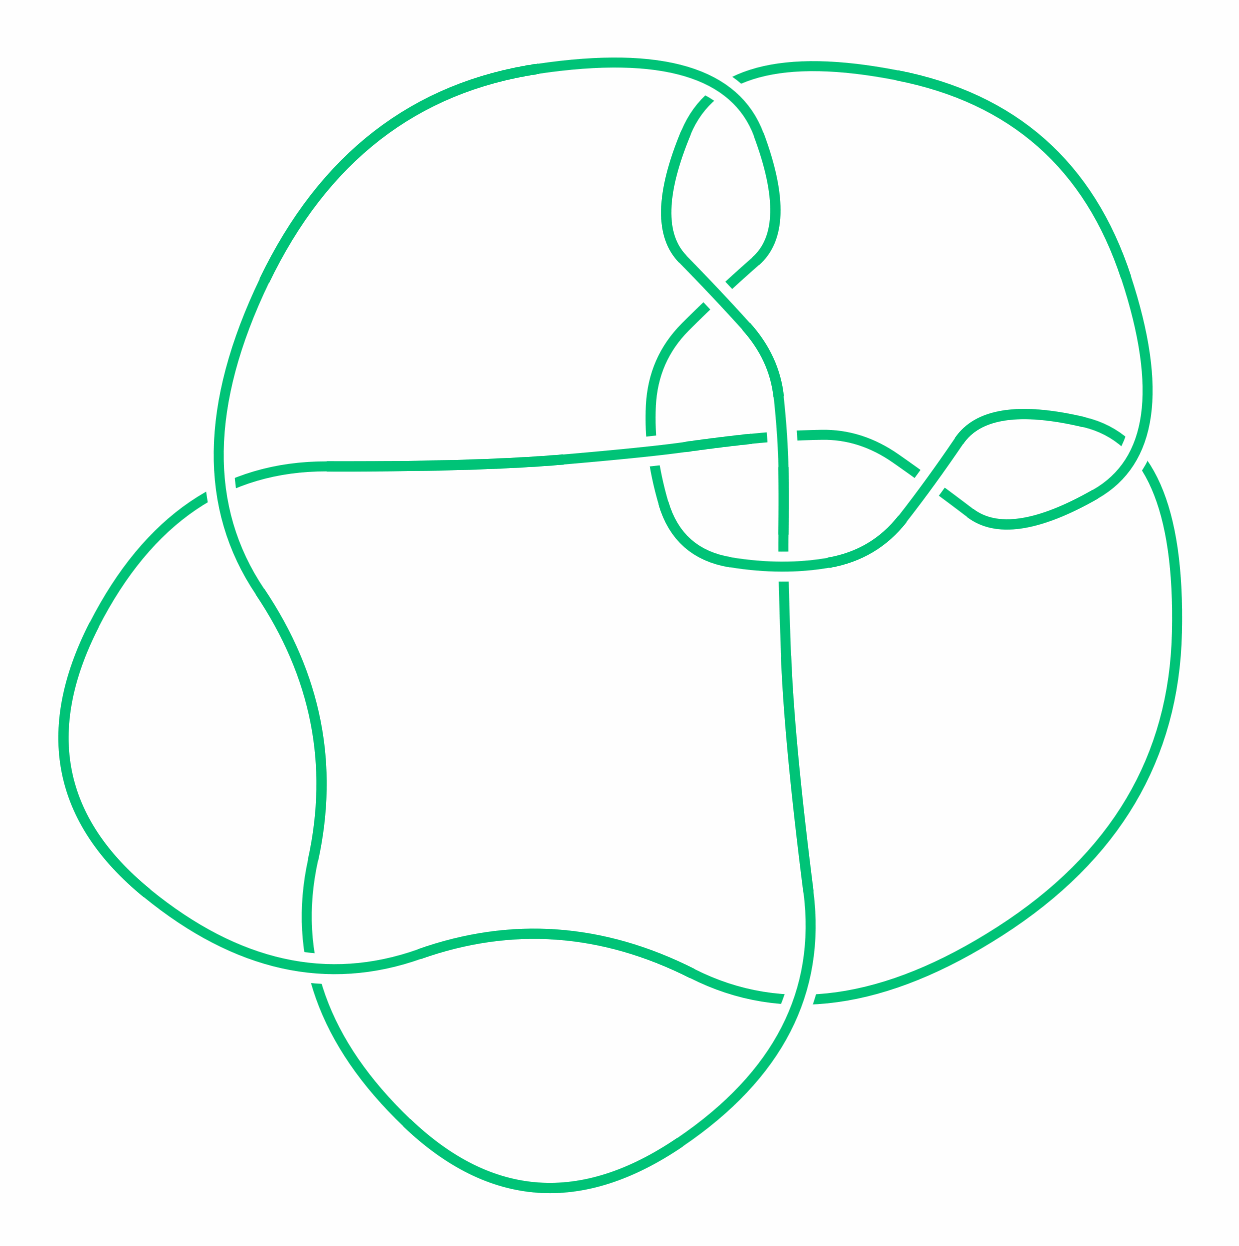
\includegraphics[width=\linewidth]{../data/perko1.png}
        \subcaption{$10_{161}$}
    \end{minipage}
    \begin{minipage}[b]{.14\linewidth}
        \centering
        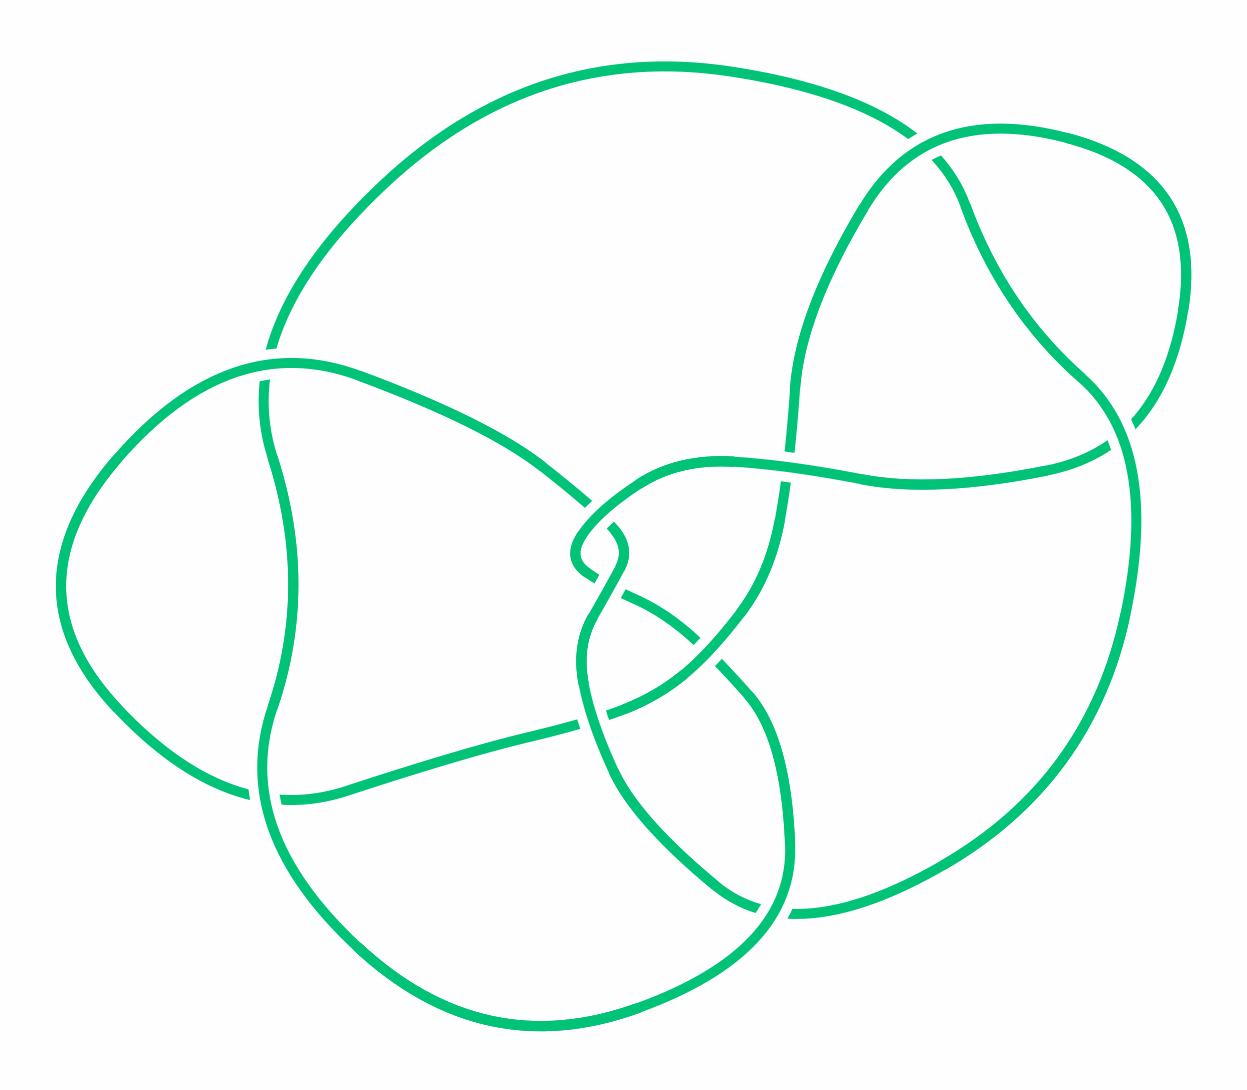
\includegraphics[width=\linewidth]{../data/perko2.png}
        \subcaption{$10_{162}$}
    \end{minipage}
\end{figure}
\end{comment}

Początkowo celem teorii węzłów była klasyfikacja wszystkich węzłów.
Od XIX wieku, kiedy teoria węzłów wyodrębniła się jako osobny dział matematyki, zdążyliśmy skatalogować ponad sześć miliardów tych obiektów.
Pozornie tak samo wyglądające węzły mogą się od siebie różnić.
Do wykrywania tych subtelnych różnic używa się przede wszystkim niezmienników topologicznych takich jak liczby, wielomiany bądź grupy.
Poznamy je w~dalszych rozdziałach.

Matematycy uogólnili pojęcie węzła: można rozpatrywać je w~wyższych wymiarach albo zastąpić okrąg inną przestrzenią topologiczną.
Będziemy starać się unikać tych uogólnień.


\section{Węzły i~sploty}
Wprowadzamy pojęcia węzła i splotu, fundamentalnych obiektów teorii, o której napisana została ta książka.
Oprócz tego podajemy definicję, kiedy dwa węzły lub sploty uznajemy za tożsame oraz uzasadniamy, dlaczego akurat ta definicja jest właściwa.

Istnieją odnogi teorii węzłów, które badają inne, pokrewne obiekty.
Mamy na przykład węzły obramowane:

% DICTIONARY;framed;obramowany;węzeł
% GLOSSAIRE;encadré;obramowany;węzeł
% DICTIONARY;framing;obramowanie;-
% GLOSSAIRE;encadrement;obramowanie;-
\begin{definition}[obramowanie]
\index{obramowanie|see {węzeł obramowany}}%
\index{węzeł!obramowany}%
    Każde nieznikające normalne pole wektorowe $V$ na splocie $L$ nazywamy jego obramowaniem.
    Szczególnie interesujący jest przypadek, gdy wszystkie wektory tego pola są równoległe do płaszczyzny, na której leży diagram tego splotu.
\end{definition}

% DICTIONARY;virtual;wirtualny;węzeł
% GLOSSAIRE;virtuel;wirtualny;węzeł
% DICTIONARY;welded;zespawany;węzeł
% GLOSSAIRE;soudé;zespawany;węzeł
% DICTIONARY;long;długi;węzeł
% GLOSSAIRE;long;długi;węzeł
Są jeszcze węzły wirtualne, zespawane (iloraz węzłów wirtualnych przez ruch znany jako ,,nadskrzyżowania komutują''), długie (gdzie końce nie są ze sobą zszyte, ale umieszczone tak daleko, że są nieosiągalne) i inne.
% http://katlas.math.toronto.edu/ester/weldedknots/explanations.html => because the "overcrossings commute" move is not symmetric
\index{węzeł!wirtualny}%
\index{węzeł!zespawany}%
\index{węzeł!długi}%
Ta książka nie zawiera zbyt wiele informacji o wspomnianych bytach.


\subsection{Węzły}
Matematyczne węzły można traktować jako model elastycznej oraz pozbawionej grubości liny, której luźne końce zostały ze sobą połączone.
Sugeruje to przyjęcie naiwnej definicji:

\begin{definition}[węzeł (prawie)]
\index{węzeł}%
    Ciągłe oraz różnowartościowe odwzorowanie $S^1 \to \R^3$ nazywamy węzłem.
\end{definition}

Takie rozwiązanie nie jest doskonałe, ponieważ oprócz pożądanych (cokolwiek to znaczy) węzłów, obejmuje wiele innych, patologicznych obiektów takich jak ten z~rysunku \ref{fig_wild_knot}.

\begin{figure}[H]
    \centering
\begin{comment}
    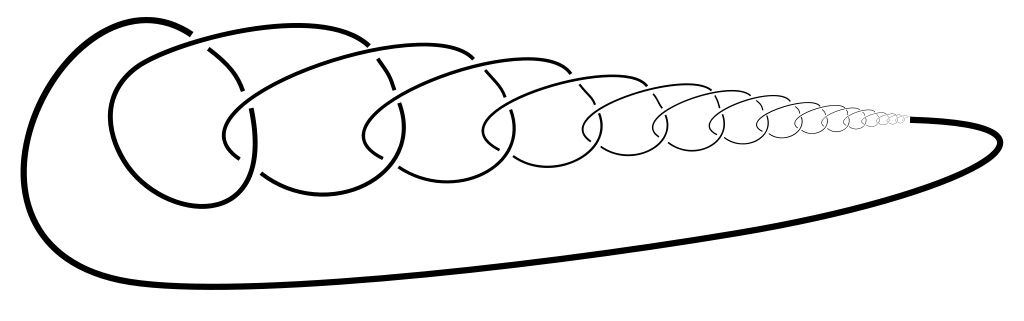
\includegraphics[height=0.14\linewidth]{wild_knot.png}
\end{comment}
    \caption[caption-wild-knot]{Węzeł dziki, źródło: Wikimedia{\footnotemark}}
\index{węzeł!dziki}%
\label{fig_wild_knot}%
\end{figure}
\footnotetext{\url{https://upload.wikimedia.org/wikipedia/commons/2/2f/Wildknot.svg}}

Zamiast wyjaśnić, jakie są jego niepożądane właściwości, podamy od razu dobrą definicję.

\begin{definition}[węzeł]
    Różnowartościowe włożenie $S^1 \to \R^3$, którego pochodna istnieje wszędzie i~nie znika nigdzie, nazywamy węzłem.
\end{definition}

\begin{example}[niewęzeł]
    Węzeł zadany w przestrzeni $\R^3$ parametrycznie $(\sin \theta, \cos \theta, 0)$ dla $\theta \in [0, 2\pi]$ nazywamy niewęzłem i oznaczamy $\SmallUnknot$.
\end{example}

Potrzeba jeszcze matematycznego opisu manipulacji, jakim możemy poddawać sznur trzymany w~ręce.
Izotopia jest niewłaściwym narzędziem do tego celu: powiedzielibyśmy, że dwa węzły $K_1, K_2$ są izotopijne, jeśli istnieje ciągła funkcja
\begin{equation}
    F \colon S^1 \times [0, 1] \to \R^3
\end{equation}
taka, że $K_1 = F(-, 0)$ jest pierwszym, zaś $K_2 = F(-,1)$ drugim węzłem (funkcję $F$ nazywa się izotopią).
Tym razem źródło problemów można wskazać jawnie.
Dowolny zaplątany fragment z węzła można usunąć wykonując sztuczkę Alexandera (ponieważ jak powiedziałyby mądre głowy, ,,przestrzeń homeomorfizmów dysku w siebie $D^{n+1} \to D^{n+1}$, które zgadzają się z odwzorowaniem tożsamościowym na brzegu dysku -- sferze $S^n$, jest spójna''):
\index[persons]{Alexander, James}%
\index{sztuczka Alexandera}%

\begin{comment}
\begin{figure}[H]
    \centering
    \fbox{\begin{minipage}[b]{.12\linewidth}
        \centering
        
\includegraphics[width=\linewidth]{../data/alexander-trick/0.png}
        \subcaption{$t = 0$}
    \end{minipage}}\,\,
    \fbox{\begin{minipage}[b]{.12\linewidth}
        \centering
        
\includegraphics[width=\linewidth]{../data/alexander-trick/1.png}
        \subcaption{$t = 1/4$}
    \end{minipage}}\,\,
    \fbox{\begin{minipage}[b]{.12\linewidth}
        \centering
        
\includegraphics[width=\linewidth]{../data/alexander-trick/2.png}
        \subcaption{$t=1/2$}
    \end{minipage}}\,\,
    \fbox{\begin{minipage}[b]{.12\linewidth}
        \centering
        
\includegraphics[width=\linewidth]{../data/alexander-trick/3.png}
        \subcaption{$t=3/4$}
    \end{minipage}}\,\,
    \fbox{\begin{minipage}[b]{.12\linewidth}
        \centering
        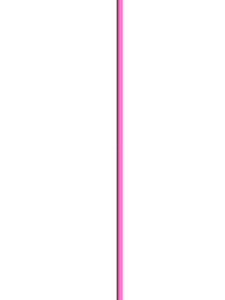
\includegraphics[width=\linewidth]{../data/alexander-trick/4.png}
        \subcaption{$t = 1$}
    \end{minipage}}
    \caption[caption-alexander-trick]{Sztuczka Alexandera}
\end{figure}
\end{comment}

W podobny sposób moglibyśmy przekształcić dowolny węzeł w~niewęzeł.
Teoria, w~której wszystkie obiekty są takie same, nie jest zbyt ciekawa.
Od izotopii należy wymagać gładkości albo lokalnej płaskości,
% https://math.stackexchange.com/questions/1311865/equivalence-of-knots-ambient-isotopy-vs-homeomorphism
co zdaje się prowadzić do pojęcia izotopii otaczającej, która uwzględnia nie tylko sam węzły, ale też to, jak leżą w otaczającej je przestrzeni.

% DICTIONARY;isotopy;izotopia;-
% GLOSSAIRE;isotopie;izotopia;-
% DICTIONARY;ambient;otaczająca;izotopia
% GLOSSAIRE;ambiante;otaczająca;izotopia
\begin{definition}[izotopia otaczająca]
    \index{izotopia otaczająca}%
    Niech $K_1, K_2 \colon N \hookrightarrow M$ będą włożeniami dwóch rozmaitości $N, M$.
    Ciągłe odwzorowanie $F \colon M \times [0,1] \to M$ spełniające następujące warunki:
    \begin{enumerate}
        \item funkcja $F(-, 0)$ jest odwzorowaniem tożsamościowym,
        \item każda z~funkcji $F(-, t)$ jest homeomorfizmem,
        \item złożenie $F(-, 1)$ z~pierwszym włożeniem $K_1$ daje drugie włożenie $K_2$
    \end{enumerate}
    nazywamy izotopią otaczającą przenoszącą włożenie $K_1$ na $K_2$.
\end{definition}

W~topologii rozważa się włożenia dowolnych rozmaitości, nam wystarczy jeden szczególny przypadek $N = S^1$ oraz $M = \R^3$.
Intuicyjnie, funkcja $F$ zniekształca przestrzeń $\R^3$ tak, że w~chwili początkowej $t = 0$ widzimy pierwszy, zaś w~chwili końcowej $t = 1$ drugi węzeł.
Izotopia otaczająca nie pozwala na ściąganie zaplątanych fragmentów do punktu.

\begin{definition}
    Dwa węzły są równoważne wtedy i tylko wtedy, gdy istnieje pomiędzy nimi izotopia otaczająca.
\end{definition}

Znając już izotopię otaczającą, można podać alternatywny opis węzłów:

% DICTIONARY;knot;węzeł;-
% GLOSSAIRE;nœud;węzeł;-
% DICTIONARY;tame;poskromiony;węzeł
% GLOSSAIRE;lisse/régulier;poskromiony;węzeł
% DICTIONARY;wild;dziki;węzeł
% GLOSSAIRE;sauvage;dziki;węzeł
\begin{definition}[węzeł]
\index{węzeł!poskromiony}%
\label{def:knot}%
    Gładkie włożenie $S^1 \hookrightarrow \R^3$ otaczająco izotopijne z~zamkniętą łamaną bez samoprzecięć nazywamy węzłem poskromionym.
\end{definition}

Czasami wygodniej jest rozpatrywać węzeł jako włożenie $S^1 \hookrightarrow S^3$ albo dopuścić do myśli węzły nieposkromione.
Ale jeśli nie zaznaczono inaczej, nie robimy tego: pisząc węzeł mamy na myśli poskromione włożenie w przestrzeń $\R^3$, nie $S^3$.

Formalnie węzły to pewne odwzorowania, więc prawidłowym sposobem na zapisanie, że są izotopijne (czyli dla nas: równe), jest $K_1 \cong K_2$.
Ponieważ nie prowadzi to do problemów, będziemy jednak stosować zapis $K_1 = K_2$.
Jednocześnie często węzeł jako odwzorowanie nie będzie odróżniany od obrazu tego odwzorowania.

Istnieje jeszcze jedna, konkurencyjna definicja węzłów równoważnych:

\begin{proposition}
\label{def:equivalent_knots_2}%
    Dwa węzły są równoważne wtedy i~tylko wtedy, gdy jeden z~nich jest obrazem drugiego przez zachowujący orientację homeomorfizm $\R^3 \to \R^3$.
\end{proposition}

\begin{proof}
    Podany niżej dowód pochodzi z~książki ,,Topology from the differentiable viewpoint'' Johna Milnora.
\index[persons]{Milnor, John}%
    Musimy pokazać, że dyfeomorfizm $f \colon \R^m \to \R^m$ jest gładko izotopijny z~identycznością.
    Translacje są izotopiami, więc bez straty ogólności zakładamy, że $f(0) = 0$.
    Pochodna $f$ w~zerze jest dana wzorem $\mathrm{d}f_0(x) = \lim_{t \to 0} f(tx) /t$, więc
    \begin{equation}
        F(x, t) = \begin{cases}
            \mathrm{d}f_0(x) & t = 0 \\
            f(tx) / t & 0 < t \le 1
        \end{cases} .
    \end{equation}
    stanowi naturalną definicję izotopii $F \colon \R^m \times [0, 1] \to \R^m$.
    Funkcja $f$ zapisuje się na mocy lematu Hadamarda jako suma $x_1 g_1(x) + \ldots + x_mg_m(x)$, gdzie funkcje $g_i$ są gładkie, więc funkcja $F$ też jest gładka, co jakoś kończy dowód.
\index{lemat Hadamarda}%    
\end{proof}

Milnor zauważa, że istnieje dyfeomorfizm $S^6 \to S^6$ stopnia $+1$, który nie jest gładko izotopijny z~identycznością!
\index[persons]{Milnor, John}%

\begin{remark}[John Willard Milnor]
    Matematyk amerykański urodzon w 1931 roku w Orange, New Jersey.
    Odkrył egzotyczną 7-wymiarową sferę (czyli zwykłą sferę z niezwykłą strukturą różniczkową) w 1956 roku, za co został później odznaczon medalem Fieldsa.
    Obalił Hauptvermutung pięć lat później: hipotezę Steinitza i Tietzego z 1908 roku, że każde dwie triangulacje przestrzeni mają kombinatorycznie równoważne podpodziały.
    Do jego zainteresowań należą topologia różniczkowa, algebraiczna K-teorią, ale też algebry Hopfa, grupy Liego i holomorficzne układy dynamiczne.
    W~świecie węzłów jest znany przez wprowadzenie niezmienników $\mu$ Milnora, które uogólniają grupę podstawową dopełnienia oraz pewne wyniki dotyczące hipotezy plastrowo-taśmowej.
\end{remark}
\index{niezmiennik!$\mu$ Milnora}%
\index{hipoteza!plastrowo-taśmowa}%
\index[persons]{Milnor, John}%




\subsection{Sploty}
% DICTIONARY;link;splot;-
% GLOSSAIRE;un entrelacs;splot;-
% DICTIONARY;component;ogniwo splotu;-
% GLOSSAIRE;composante/boucle;ogniwo splotu;-
\begin{definition}[splot, ogniwo]
\index{splot}%
    Sumę parami rozłącznych węzłów
    \begin{equation}
        L = K_1 \sqcup K_2 \sqcup \ldots K_n
    \end{equation}
    nazywamy splotem, a~składniki $K_i$ -- ogniwami splotu.
\end{definition}

Przez analogię do węzłów mówimy, że dwa sploty są takie same, jeśli jeden jest obrazem drugiego przez zachowujący orientację homeomorfizm $\R^3 \to \R^3$.
To oczywiste, że liczba ogniw jest niezmiennikiem splotów.
Później podamy mniej oczywiste niezmienniki.

\begin{example}[niesplot]
\index{niesplot}%
    Splot zadany w przestrzeni $\R^3$ parametrycznie
    \begin{equation}
        \bigcup_{k=1}^n \{(\sin \theta, \cos \theta, k) : \theta \in [0, 2\pi]\}
    \end{equation}
    nazywamy niesplotem i oznaczamy $U_n$.
\end{example}
    
\begin{example}
\index{splot!Hopfa}%
\index[persons]{Hopf, Heinz}%
    Splot Hopfa (rys. \ref{small_links_diagram}a), najprostszy nietrywialny splot. Ma dwa ogniwa.
\end{example}

\begin{remark}[Heinz Hopf]
    Matematyk niemiecki urodzon w 1894 roku w Gräbschen (obecnie część Wrocławia); zmarł w 1971 roku w Zurychu, Szwajcarii.
    Głównym wynikiem jego pracy doktorskiej z~1925 roku było, że każda jednospójna zupełna 3-rozmaitość Riemanna o~stałej krzywiźnie sekcyjnej jest globalnie izometryczna do przestrzeni euklidesowej, sferycznej lub hiperbolicznej.
    Był pionierem topologii algebraicznej.
    W~1931 roku prowadził badania nad tzw. rozwłóknieniem: odwzorowaniem $S^3 \to S^2$ takim, że przeciwobrazy punktów są okręgami wielkimi na 3-sferze.
    Podczas tych badań zajmował się splotem nazywanym teraz splotem Hopfa.
\end{remark}

\begin{example}
\index{splot!Whiteheada}%
\index[persons]{Whitehead, John}%
    Splot Whiteheada (rys. \ref{small_links_diagram}b).
\end{example}

\begin{remark}[John Henry Constantine Whitehead]
    Matematyk brytyjski urodzon w 1903 roku w~Madrasie, Indiach; zmarł w 1960 roku w Princeton, New Jersey.
    Był jednym z założycieli teorii homotopii, podał definicję CW-kompleksów.
    Próbował udowodnić hipotezę Poincarégo, ale popełnił błąd twierdząc, że nie istnieje ściągalna otwarta 3-rozmaitość, która nie jest homeomorficzna z $\R^3$.
    W 1935 roku sam wskazał taką rozmaitość, do jej konstrukcji wykorzystując splot Whiteheada.
\end{remark}

\begin{comment}
    \begin{figure}[H]
        \centering
        \begin{minipage}[b]{.3\linewidth}
            \centering
            
\includegraphics[height=0.6\linewidth]{../data/links/2_2_1.png}
            \subcaption{splot Hopfa}
        \end{minipage}\,\,
        \begin{minipage}[b]{.3\linewidth}
            \centering
            
\includegraphics[height=0.6\linewidth]{../data/links/5_2_1.png}
            \subcaption{splot Whiteheada}
        \end{minipage}\,\,
        \begin{minipage}[b]{.3\linewidth}
            \centering
            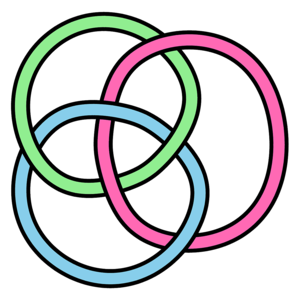
\includegraphics[height=0.6\linewidth]{../data/links/6_3_2.png}
            \subcaption{pierścienie Boromeuszy}
            \index{pierścienie Boromeuszy}%
        \end{minipage}
        \caption[small-links]{Sploty o małej liczbie skrzyżowań}
        \label{small_links_diagram}
    \end{figure}
\end{comment}


\subsubsection{Sploty rozszczepialne}
Aby wytłumaczyć, czemu trzeci splot z rysunku \ref{small_links_diagram} jest interesujący, potrzebujemy zdefiniować sploty rozszczepialne.

% DICTIONARY;splittable;rozszczepialny;splot
\begin{definition}[rozszczepialność]
\index{splot!rozszczepialny}%
    Jeżeli splot $L$ można zanurzyć w przestrzeni $\R^3$ tak, że niektóre jego ogniwa będą leżeć nad pewną rozłączną ze splotem płaszczyzną, zaś pozostałe pod nią, to powiemy, że splot $L$ jest rozszczepialny.
\end{definition}

Liczbę nierozszczepialnych splotów pierwszych kopiujemy z bazy danych LinkInfo \cite{linkinfo24}:
\renewcommand*{\arraystretch}{1.4}
\footnotesize
\begin{longtable}{lcccccccccccc}
    \hline
    \textbf{skrzyżowania} & 0 & 1 & 2 & 3 & 4 & 5 &  6 &  7 &  8 & 9 & 10 & 11 \\ \hline \endhead
    sploty pierwsze, nierozszczepialne & 0 & 0 & 1 & 0 & 1 & 1 & 6 & 9 & 29 & 83 & 287 & 1007 \\
    (w tym) alternujące & 0 & 0 & 1 & 0 & 1 & 1 & 5 & 7 & 21 & 55 & 174 & 548 \\
    (w tym) niealternujące & 0 & 0 & 0 & 0 & 0 & 0 & 1 & 2 & 8 & 28 & 113 & 459 \\
    \hline
\end{longtable}
\normalsize

W bazie liczb OEIS trafiliśmy tylko na ciąg \href{https://oeis.org/A086826}{A086826} opisujący liczbę nierozszczepialnych pierwszych i złożonych węzłów i splotów, na przykład $a_5 = 4$, bo mamy dwa węzły pierwsze, splot Whiteheada oraz trójlistnik spleciony z~niewęzłem.
Słowa ,,skrzyżowanie'' , ,,alternujący'' oraz ,,pierwszy'' definiujemy w~przyszłości, będą to odpowiednio definicje \ref{def:crossing}, \ref{def:alternating_link} i \ref{def:prime_knot}.
\index{węzeł!alternujący}%
\index{węzeł!pierwszy}%
\index{skrzyżowanie}%
Książka ma nieliniową budowę i należy przeczytać ją co najmniej dwa razy.

Pewne kryteria rozszczepialności konkretnych splotów znaleźć można u Kawauchiego \cite[s. 36-38]{kawauchi1996}.
% przepisać, a jeśli za trudne, to może chociaż szkic?




\subsubsection{Sploty Brunna}
\index{splot!Brunna|(}%
Hermann Brunn \cite{brunn1892} rozpatrywał w 1892 roku (a więc zanim jeszcze teoria węzłów przyszła na świat!) nierozszczepialne sploty, które po usunięciu dowolnego ogniwa stają się niesplotami.
\index[persons]{Brunn, Hermann}%
W~czasopiśmie Delta, nr 01/2011, przeczytaliśmy, że Rolfsen zaproponował nazywać je splotami Brunna i~tak też będziemy robić.
Najprostszym splotem Brunna są posiadające trzy ogniwa pierścienie Boromeuszy ($6_2^3$ w notacji Alexandera-Briggsa, \texttt{L6a4} w notacji Thistlethwaite'a).
\index{pierścienie Boromeuszy}%
Pokażemy na stronie \pageref{boromean_not_splittable}, że pierścienie Boromeuszy nie mają nietrywialnych trójkolorowań, więc nie mogą być niesplotem.

Pierścienie Boromeuszy są alternujące, hiperboliczne i drzewiaste.
\index{węzeł!alternujący}%
\index{węzeł!hiperboliczny}%
\index{węzeł!drzewiasty}%
% DICTIONARY;arborescent;drzewiasty;węzeł
% TODO: jak jest arborescent po francusku?
Ich nazwa pochodzi od lombardzko-piemonckiego rodu kupieckiego, bankierskiego i arystokratycznego, z którego wywodziło się wielu kardynałów.
Herb tego rodu zawierał splecione ze sobą trzy okręgi.
Jest niemożliwe, by wykonać model przestrzenny tego splotu przy użyciu okrągłych pierścieni.
Zamiast tego można użyć na przykład elips.

Z dokładnością do homotopii sploty Brunna zostały sklasyfikowane przez Milnora \cite{milnor1954}, ale ponieważ ta książka nie tłumaczy, czym są $\mu$-niezmienniki Milnora, nie możemy dzisiaj wytłumaczyć, jak tego dokonał.
\index[persons]{Milnor, John}%
\index{splot!Brunna|)}%




\subsubsection{Sploty alternujące}

Zazwyczaj do zdefiniowania splotów alternujących potrzebne są najpierw diagramy.
% Zanim opowiemy, jak dotąd przebiegała klasyfikacja węzłów o małej liczbie skrzyżowań, zdefiniujemy klasę splotów ze specjalnymi diagramami.

% DICTIONARY;alternating;alternujący;węzeł
\begin{definition}[splot alternujący]
\label{def:alternating_link}%
\index{węzeł!alternujący}%
    Niech $D$ będzie diagramem splotu $L$.
    Jeżeli podczas poruszania się wzdłuż każdego ogniwa naprzemiennie mijamy podskrzyżowania oraz nadskrzyżowania, to diagram nazywamy alternujący.
    
    Splot $L$ jest alternujący, jeśli posiada alternujący diagram $D$s.
\end{definition}

Około 1961 roku Ralph Fox zapytał \emph{,,What is an alternating knot?''}.
\index[persons]{Fox, Ralph}%
Szukano takiej definicji węzła alternującego, która nie odnosi się bezpośrednio do diagramów, aż w~2015 roku Greene \cite{greene2017} podał geometryczną charakteryzację: nierozszczepialny splot w $S^3$ jest alternujący wtedy i~tylko wtedy, gdy ogranicza dodatnią oraz ujemną określoną powierzchnię rozpinającą.
\index[persons]{Greene, Joshua}%

\begin{remark}[Ralph Hartzler Fox]
    Matematyk amerykański urodzon w Morrisville, Pensylwanii w~1913 roku; zmarł w Filadelfii, tamże w 1973 roku.
    Był promotorem Johna Milnora, Lee Neuwirtha (o~których jeszcze wspomnimy!) i 23 innych osób, o których nie wspomnimy.
    Oprócz tego nadzorował pracę licencjacką Kennetha Perko.
    Zawdzięczamy mu spopularyzowanie $n$-kolorowania na koledżu Haverford w 1956 roku, podanie nowego sposobu na znalezienie wielomianu Alexandera przy użyciu rachunku różniczkowego Foxa oraz niektóre terminy teorii węzłów uzywane po dziś dzień: węzeł plastrowy, węzeł taśmowy, okrąg i powierzchnia Seiferta.
\end{remark}

Nie ma zwartego wzoru na liczbę splotów alternujących, ale wiemy, że rośnie co najmniej wykładniczo względem liczby skrzyżowań:

\begin{proposition}
\index{supeł}%
    Niech $a_n$ oznacza liczbę supłów o~$n$ skrzyżowaniach, które są alternujące oraz pierwsze.
    Wtedy
    \begin{equation}
        a_n \sim \frac{3c_1 \lambda^{n-3/2}}{4\sqrt{\pi n^{5}}},
    \end{equation}
    gdzie zarówno $c_1$, pierwszy współczynnik rozwinięcia Taylora funkcji $\Phi(\eta)$ zdefiniowanej w \cite{sundberg1998}, jak i $\lambda$ są jawnie znanymi stałymi:
    \begin{align}
        c_1 & = \sqrt{\frac{5^7 \cdot (21001 + 371 \sqrt{21001})^3}{2 \cdot 3^{10} \cdot (17 + 3\sqrt{21001})^5}} \\
        \lambda & = \frac {1}{40} (101 + \sqrt{21001})
    \end{align}
    Niech $A_n$ oznacza liczbę pierwszych, alternujących splotów o $n$ skrzyżowaniach.
    Wtedy $A_n \approx \lambda^n$, dokładniej: jeśli $n \ge 3$, to
    \begin{equation}
        \frac{a_{n-1}}{16n - 24} \le A \le \frac{a_n - 1}{2}.
    \end{equation}
\end{proposition}

Węzły pierwsze i~supły pojawiają się odpowiednio w definicjach \ref{def:prime_knot}, \ref{def:tangle}.

\begin{proof}[Niedowód]
\index[persons]{Sundberg, Carl}%
\index[persons]{Thistlethwaite, Morwen}%
    Zamiast przedstawić dowód albo chociaż jego szkic, wymienimy trzy narzędzia użyte przez Sundberga, Thistlethwaite'a \cite{sundberg1998}:
    algebraiczną metodę Conwaya znajdowania splotów,
    wynik Tuttego dotyczącego liczby ukorzenionych $c$-sieci
    oraz (wtedy już udowodnioną) hipotezę Taita.
\index[persons]{Conway, John}%
\index[persons]{Tutte, William}%
\index{hipoteza!Taita}%
\end{proof}

\begin{proposition}
    Niech $a_n$ oznacza liczbę supłów o~$n$ skrzyżowaniach, które są alternujące oraz pierwsze.
    Wtedy funkcja tworząca $f(z) = \sum_n a_n z^n$ spełnia równanie
    \begin{equation}
    f(1+z) - f(z)^2 - (1+f(z))q(f(z)) -z - \frac{2z^2}{1-z} = 0,
    \end{equation}
    gdzie $q(z)$ jest pomocniczą funkcją
    \begin{equation}
        q(z) = \frac{2z^2 - 10z - 1 + \sqrt{(1-4z)^3}} {2(z+2)^3} - \frac{2}{1+z} -z + 2.
    \end{equation}
\end{proposition}

Powyższa ciekawostka także pochodzi z cytowanej wcześniej pracy \cite{sundberg1998}.





\subsection{Dopełnienia węzłów i splotów}
Jeśli dwa węzły są równoważne, to ich dopełnienia są oczywiście homeomorficzne.
Pytanie o~prawdziwość implikacji odwrotnej jako pierwszy zadał najprawdopodobniej Tietze \cite{tietze1908} w~1908 roku.
\index[persons]{Tietze, Heinrich}%
O~jego trudności niech świadczy fakt, że dopiero w~roku 1987 pokazano, że istnieją co najwyżej dwa węzły o~zadanym dopełnieniu (Culler, Gordon, Luecke, Shalen \cite{culler1987}).
\index[persons]{Culler, Marc}%
\index[persons]{Shalen, Peter}%
\index[persons]{Gordon, Cameron}%
\index[persons]{Luecke, John}%
Dwa lata później poznaliśmy pozytywną odpowiedź na pytanie Tietzego: każdy węzeł jest wyznaczony jednoznacznie przez swoje dopełnienie.
Natomiast analogiczne stwierdzenie o~splotach jest fałszywe i wiedziano o tym od bardzo dawna: w~1937 roku Whitehead \cite{whitehead1937} podał nieskończenie wiele splotów, których dopełnienia wyglądają jak dopełnienia splotu Whiteheada.

\begin{theorem}[Gordon, Luecke, 1989]
\index[persons]{Gordon, Cameron}%
\index[persons]{Luecke, John}%
\index{twierdzenie!Gordona-Lueckego}%
    Niech $f \colon (\mathbb R^3 \setminus K_1) \to (\mathbb R^3 \setminus K_2)$ będzie zachowującym orientację homeomorfizmem dopełnień poskromionych węzłów $K_1, K_2$.
    Wtedy węzły $K_1 \cong K_2$ są izotopijne.
\end{theorem}

\begin{proof}[Niedowód]
    Wynika to z teorii Cerfa, kombinatorycznych technik w stylu Litherlanda, cienkich pozycji, cykli Scharlemanna i~ogólniejszego stwierdzenia: nietrywialna chirurgia Dehna na węźle w~3-sferze nigdy nie daje 3-sfery.
\index{chirurgia Dehna}%
\index{cykle Scharlemanna}%
\index{teoria Cerfa}%
    Pełny dowód zawiera praca \cite{gordon1989}.
\end{proof}

Twierdzenie to zamienia problem lokalny (czy dwa węzły w kuli $S^3$ są równoważne?) na problem globalny (czy dwie przestrzenie topologiczne są homeomorficzne?).
\index[persons]{Whitehead, John}%

% koniec sekcji Węzły i sploty



\section{Diagramy. Ruchy Reidemeistera}

Chociaż w~świetle definicji \ref{def:knot} węzły są pewnymi regularnymi podzbiorami przestrzeni $\R^3$, z~kombinatorycznego punktu widzenia wygodniej jest rysować je na płaszczyźnie.

% DICTIONARY;shadow;cień;-
% DICTIONARY;crossing;skrzyżowanie;-
\begin{definition}[cień, skrzyżowanie]
\index{cień}%
\index{skrzyżowanie}%  
\label{def:crossing}%
    Niech $\pi \colon \R^3 \to \R^2$ będzie rzutem na pewną płaszczyznę, zaś $L \subseteq \R^3$ ustalonym splotem.
    Obraz $\pi[L]$ nazywamy cieniem, punkty podwójne $p$ cienia (punkt $p \in \R^2$, którego przeciwobraz $\pi^{-1}[\{p\}]$ jest dwupunktowy) nazywamy skrzyżowaniami.
\end{definition}

\begin{definition}[diagram]
% DICTIONARY;diagram;diagram;-
\index{diagram}%
    Niech $D$ będzie cieniem splotu $L$ takim, że cień $D$ zawiera skończenie wiele punktów wielokrotnych (i wszystkie są punktami podwójnymi) oraz skrzyżowania cienia $D$ nie zawierają wierzchołków splotu $L$.
    Wtedy cień $D$ wzbogacony o~informację o tym, jak przebiegają skrzyżowania (który odcinek łamanej biegnie dołem, a~który górą) nazywamy diagramem.
% TODO: dopisać, że będziemy to nazywać nad i pod skrzyżowania
\index{nadskrzyżowanie}%
\index{podskrzyżowanie}%
\end{definition}

Mieliśmy problemy ze znalezieniem ładnego rysunku katastrof, jakich nie dopuszczamy pracując z diagramami zamiast zwykłymi cieniami; nam nie do końca chciało się je rysować je tutaj.
Wybawieniem okazała się monografia Burdego, Zieschanga (i Heusenera) \cite[s. 9]{burde2014}.

Dla każdego ustalonego $n \ge 2$ i każdego węzła $K$ istnieje cień $D$, na którym wszystkie wielokrotne punkty są $n$-krotne (wiemy to od Hostego, College'a \cite[s. 11]{adams2021}, którzy nie napisali, skąd to wiedzą);
\index[persons]{Hoste, Jim}%
\index[persons]{College, Pitzer}%
dla co najmniej jednej wartości $n$ można dodatkowo wymagać, by diagram zawierał dokładnie jedno skrzyżowanie (Adams, Crawford, DeMeo, Landry, Lin, Montee, Park, Venkatesh, Yhee \cite{venkatesh2015} albo Brunn ponad sto lat temu \cite[s. 28]{adams2021}!).
\index[persons]{Adams, Colin}%
\index[persons]{Crawford, Thomas}%
\index[persons]{DeMeo, Benjamin}%
\index[persons]{Landry, Michael}%
\index[persons]{Lin, Alex}%
\index[persons]{Montee, Murphy}%
\index[persons]{Park, Seojung}
\index[persons]{Venkatesh, Saraswathi}%
\index[persons]{Yhee, Farrah}%

\begin{definition}[włókno, nić]
\index{włókno}%
\index{nić}%
    Fragment diagramu biegnący między dwoma kolejnymi skrzyżowaniami (odpowiednio: tunelami, czyli podskrzyżowaniami), nazywamy nicią (odpowiednio: włóknem)
\end{definition}

Skrzyżowania i diagramy są standardowymi terminami, zrozumiałymi przez każdego. 
Cienie, nici i włókna stanowią twórczość własną autorów!
Nici powstają z włókien przez rozcięcie ich przy każdym nadskrzyżowaniu.

\begin{proposition}
\label{prp:links_have_diagrams}%
    Niech $L$ będzie splotem.
    Jego diagramy tworzą otwarty i~gęsty podzbiór wszystkich rzutów.
\end{proposition}

Kawauchi \cite[s. 7]{kawauchi1996} wspomina w tym miejscu podręcznik Crowella, Foxa \cite[s. 7]{crowell1963}.
To samo jest na przykład u Burdego, Zieschanga, Heusenera \cite[s. 10]{burde2014}, ale oni odsyłają jeszcze do Reidemeistera \cite{reidemeister1927} i samego Burdego \cite{burde1978}.

\begin{proof}[Niedowód]
    Rzut splotu na równoległe płaszczyzny jest taki sam, a te można sparametryzować prostymi przechodzącymi przez początek układu współrzędnych, które tworzą przestrzeń rzutową $\R \mathbb P^2$.
    Niech $S$ będzie zbiorem prostych, które dają złe rzuty.
    Wystarczy pokazać jego nigdziegęstość.
    Okazuje się, że $S$ jest też jednowymiarowy.
\end{proof}

\begin{corollary}
    Każdy splot posiada diagram.
\end{corollary}

% DICTIONARY;oriented;zorientowany;węzeł
\begin{definition}[orientacja]
\index{węzeł!zorientowany}%
\index{orientacja|see {węzeł zorientowany}}%
    Węzeł, w~którym wybrano kierunek, w~którym należy się po nim poruszać, nazywamy zorientowanym.
    Splot nazywamy zorientowanym, jeśli wszystkie jego ogniwa traktowane jako węzły są zorientowane.
\end{definition}

Orientację na diagramie zaznaczamy małą strzałką wskazującą kierunek poruszania się.


\subsection{Ruchy Reidemeistera}

Wiemy już, że węzły mają wiele diagramów.
Mając dane dwa różne diagramy chcielibyśmy wiedzieć, czy przedstawiają ten sam węzeł.
Stosowne narzędzie dostarczył Kurt Reidemeister w~latach dwudziestych ubiegłego wieku.
\index[persons]{Reidemeister, Kurt}%
Zdefiniujmy trzy lokalne operacje na diagramach, a~potem wysłowimy kryterium  Reidemeistera rozstrzygające problem równości węzłów.

% DICTIONARY;Reidemeister/Turaev/... move;ruch Reidemeistera/Turajewa/...;-
\begin{definition}[ruchy Reidemeistera]
\index{ruch!Reidemeistera}%
    Trzy gatunki lokalnych deformacji diagramu splotu:
    \begin{figure}[H]
    \centering
    \begin{minipage}[b]{.22\linewidth}%
        \centering%
        \MedLarReidemeisterOneLeft $\stackrel{R_1}{\cong}$ \MedLarReidemeisterOneStraight%
        \subcaption{ruch $R_1$}%
    \end{minipage}
    \quad\quad\quad
    \begin{minipage}[b]{.2\linewidth}
        \centering
        \MedLarReidemeisterTwoA $\stackrel{R_2}{\cong}$ \MedLarReidemeisterTwoB
        \subcaption{ruch $R_2$}
    \end{minipage}
    \quad\quad\quad
    \begin{minipage}[b]{.32\linewidth}
        \centering
        \MedLarReidemeisterThreeA $\stackrel{R_3}{\cong}$ \MedLarReidemeisterThreeB
        \subcaption{ruch $R_3$}
    \end{minipage}
    \caption[reidemeister-moves]{Trzy ruchy Reidemeistera}
    \end{figure}
    nazywamy ruchami Reidemeistera.
    Czasami używa się konkretnych nazw:
    \begin{itemize}
        \item skręcenie/rozkręcenie (dla $R_1$),
        \item wsunięcie/rozsunięcie (dla $R_2$) oraz
        \item przesunięcie łuku przez skrzyżowanie (dla $R_3$).
    \end{itemize}
\end{definition}

Reidemeister w~swojej pierwszej pracy przyjął inną kolejność, jego drugi ruch jest naszym pierwszym.
Dzięki temu ruch $R_k$ operuje na $k$ łukach diagramu.
Colberg \cite[s. 6]{colberg2013} pisze, że Maxwell znał ruchy Reidemeistera przed Reidemeisterem, ale mimo próśb Taita nigdy nie zgłosił swojego odkrycia w Royal Society of Edinburgh.
\index[persons]{Tait, Peter}%
\index[persons]{Maxwell, James}%

\begin{theorem}[Reidemeister, 1927]
\label{thm:reidemeister}%
\index{twierdzenie!Reidemeistera}%
\index[persons]{Reidemeister, Kurt}%
    Niech $D_1, D_2$ będą diagramami dwóch splotów $L_1, L_2$.
    Sploty $L_1, L_2$ są takie same wtedy i tylko wtedy, gdy diagram $D_2$ można otrzymać z $D_1$ wykonując skończony ciąg ruchów Reidemeistera oraz gładkich deformacji łuków, bez zmiany biegu skrzyżowań.
\end{theorem}
% https://math.stackexchange.com/questions/4399634/two-knots-k-and-k-prime-are-equivalent-if-and-only-if-their-projections-p
% Reidemeister, and pretty much every other author, has worked with the piecewise-linear case. In a way it doesn't matter which you choose, since there's a theorem that the categories of smooth and PL manifolds are equivalent in some sense. However, it's not so clear how you pass from one setting to the other (or at least I've never gone through the details myself!)

Twierdzenie Reidemeistera jest prawdziwe także dla splotów zorientowanych, ale wtedy trzeba uwzględnić różne orientacje łuków i~nie jest oczywiste, ile spośród $2^1 + 2^2 + 2^3 = 14$ wersji jest potrzebne.
Polyak \cite{polyak2010} pokazał, że minimalny zbiór zorientowanych ruchów składa się na przykład z~dwóch wersji ruchu $R_1$, jednej wersji ruchu $R_2$ i~jednej wersji ruchu $R_3$.
\index[persons]{Polyak, Michael}%

\begin{proof}[Niedowód]
Dowód podali niezależnie Reidemeister \cite{reidemeister1927} oraz Alexander, Briggs \cite{alexander1927}.
\index[persons]{Reidemeister, Kurt}%
\index[persons]{Briggs, Garland}%
\index[persons]{Alexander, James}%
    Szkielet dowodu można znaleźć w~książce Burdego i~Zieschanga \cite[s. 9-11]{burde2014}, ale kluczowe pomysły podają też Prasołow z~Sosińskim \cite[s. 11-12]{prasolov1997}.
\index[persons]{Burde, Gerhard}%
\index[persons]{Zieschang, Heiner}%
\index[persons]{Prasołow, Wiktor (Прасолов, Виктор Васильевич)}%
\index[persons]{Sosiński, Aleksiej (Сосинский, Алексей Брониславович)}%
    Innym przystępnym źródłem jest podręcznik Murasugiego \cite[s. 50-56]{murasugi1996}.
\index[persons]{Murasugi, Kunio}%
\end{proof}

\begin{remark}[Kurt Werner Friedrich Reidemeister]
    Matematyk niemiecki urodzon w Brunszwiku w 1893 roku; zmarł w Getyndze w 1971 roku.
    W 1922 został nominowany na stanowisko profesora nadzwyczajnego na Uniwersytecie Wiedeńskim; nominację tę przyjął.
    To podczas pobytu tamże podjął decyzję o studiowaniu teorii węzłów, ale także poznał swoją przyszłą żonę: pochodzącą z~Rygi Elżbietę Wagner.
    W 1925 roku przeniósł się na Albertynę we (wtedy jeszcze pruskim) Królewcu, gdzie opracował kamień węgielny teorii węzłów: ruchy Reidemeistera.
    Później dokonał jeszcze kilku ciekawych odkryć: w 1935 zdefiniował niezmienniki torsyjne, które po raz pierwszy były w stanie odróżnić równoważne homotopijnie, ale nie homeomorficzne rozmaitości; konkretniej: pokazał, że przestrzenie soczewkowe $L(7, 1)$ i $L(7, 2)$ nie są homeomorficzne.
    Sklasyfikował grupy abelowe, które występują jako grupy podstawowe 3-rozmaitości i dowiódł, że każde dwa rozkłady Heegarda 3-rozmaitości mają wspólną stabilizację.
    Jednym z jego studentów był Heiner Zieschang, autor wielokrotnie cytowanej tu \cite{burde2014}.
\end{remark}

\begin{remark}[James Waddell Alexander]
    Matematyk amerykański urodzon w 1888 roku w Sea Bright, New Jersey; zmarł w 1971 roku w Princeton, też New Jersey.
    Był studentem Veblena, wspólnie z którym pokazał, że topologię rozmaitości można przenieść na wielościany.
    Przed 1920 rokiem udowodnił, że homologie kompleksów symplicjalnych są niezmiennikiem topologicznym.
    Jego pionierskie prace dotyczące topologii algebraicznej położyły fundament dla pomysłów Poincarégo.
    homologii.
    Kiedyś pomiędzy rokiem 1930 i 1935 zdefiniował kołańcuchy, co doprowadziło go do odkrycia (niezależnie od Kołmogorowa) kohomologii.
    Oprócz sztuczki Alexandera wprowadził bardzo ważny niezmiennik nazwany na jego cześć wielomianem Alexandera, moduł z gradacją otrzymany z homologii cyklicznego nakrycia dopełnienia węzła.
    Nie samą matematyką żył człowiek!
    Był miłośnikiem wspinaczki górskiej.
    Podczas pobytu w Princeton regularnie zostawiał uchylone okno w swoim gabinecie, żeby móc się do niego wdrapać.
\end{remark}

\begin{remark}[Garland Baird Briggs]
    Matematyk amerykański, urodzon w Sebrell, Wirginii w 1894 roku; zmarł w Kolumbii w 1959 roku.
    Niestety nie wiemy za dużo o tym człowieku.
\end{remark}

Trace \cite{trace1983} zauważył, że dwa diagramy jednego węzła są związane tylko II i III ruchem (ale nie I) wtedy i tylko wtedy, gdy mają ten sam spin oraz indeksy nawinięcia.
\index[persons]{Trace, Bruce}%
Z prac Östlunda \cite{ostlund2001}, Manturowa \cite[s. ???]{manturov2004} oraz Haggego \cite{hagge2006} wynika, że dla każdego węzła istnieje para diagramów, do przejścia między którymi trzeba wykorzystać wszystkie trzy ruchy.
% TODO: ustalić, które strony w Manturowie
\index[persons]{Östlund, Olof}%
\index[persons]{Manturow, Wasilij}%
\index[persons]{Hagge, Tobias}%
% praca Haggego nazywa się "Every Reidemeister move is needed for each knot type" ale nawet w MathSciNecie wspomnieni są Ostlund i Manturow, więc zostawiam. Tekst skopiowany z Wiki
Coward \cite{coward2006} zademonstrował, że nawet jeśli wszystkie trzy ruchy są potrzebne, można je wykonywać w specjalnej kolejności: najpierw tylko I ruchy, potem tylko II ruchy, następnie tylko III ruchy i~znowu II ruchy.
\index[persons]{Coward, Alexander}%

Do pokazania, że dwa węzły $K_1, K_2$ nie są równoważne, powinniśmy na mocy twierdzenia \ref{thm:reidemeister} udowodnić, że żaden ciąg ruchów Reidemeistera nie przekształca jednego w drugi.
\label{page_first_invariant}%
Oczywiście nikt o zdrowych zmysłach tak nie postępuje.
Zamiast tego wprowadza się stosowny niezmiennik, czyli funkcję $f$ określoną na zbiorze wszystkich węzłów (albo splotów, supłów, warkoczy itd.) tak, że jeśli węzły $K_1 \cong K_2$ są równoważne, to $f(K_1) = f(K_2)$.
% DICTIONARY;invariant;niezmiennik;-
Łatwo widać, że jeśli $f(K_1) \neq f(K_2)$, to węzły $K_1, K_2$ nie mogą być równoważne.
Natomiast gdy wartości są te same, nie dostajemy żadnej informacji.

Poznaliśmy jak na razie dwa niezmienniki: liczbę ogniw splotu oraz dopełnienie splotu do przestrzeni, w której jest zanurzony ($\mathbb R^3$ lub $S^3$).
Wiele, chociaż nie wszystkich, innych niezmienników definiuje się nie bezpośrednio na zbiorze węzłów, ale na zbiorze diagramów.
Należy wtedy sprawdzić, że każdy z trzech ruchów Reidemeistera nie ma wpływu na wartość niezmiennika.

Niezmienniki będą nam stale towarzyszyć w~wędrówce po krainie węzłów.

\subsubsection{Dygresja -- wyniki ilościowe wokół twierdzenia Reidemeistera}
Załóżmy, że na dwóch diagramach tego samego węzła widać odpowiednio $n_1, n_2$ skrzyżowań.
Jak piszą Coward, Lackenby \cite{coward2011}, istnieje funkcja $f \colon \N \times \N \to \N$ taka, że między dwoma diagramami można przejść wykonując co najwyżej $f(n_1, n_2)$ ruchów.
\index[persons]{Coward, Alexander}%
\index[persons]{Lackenby, Marc}%
Wynika to z faktu, że istnieje skończenie wiele spójnych diagramów o danej liczbie skrzyżowań oraz twierdzenia Reidemeistera.
Okazuje się jednak, że od funkcji $f$ można żądać, by była obliczalna
(a to jest chyba równoważne istnienia algorytmu rozpoznającego, czy dwa diagramy przedstawiają jeden węzeł)
% http://people.dm.unipi.it/martelli/Cortona/Lackenby.pdf 7 of 90
i faktycznie, główny wynik \cite{coward2011} orzeka, że
\begin{equation}
    f(n_1, n_2) = 2^{2^{\ldots^{2^{n_1 + n_2}}}}
\end{equation}
jest taką funkcją.
Piętrowa potęga liczy sobie aż $10^{1000000 (n_1 + n_2)}$ warstw.

Natomiast jeżeli $n_2 = 0$, czyli drugi diagram przedstawia niewęzeł, ,,wystarcza'' $(236n_1)^{11}$ ruchów, przy czym liczba skrzyżowań podczas transformacji nigdy nie przekracza $49c^2$: to świeższy wynik samego Lackenby'ego \cite{lackenby2015}, gdzie poprawił wcześniejsze oszacowania Hassa, Lagariasa.
\index[persons]{Hass, Joel}
\index[persons]{Lagarias, Jeffrey}%
Przykład diagramu niewęzła, do rozwiązania którego nie można tylko usuwać istniejących skrzyżowań, przedstawiają Burde, Zieschang, Heusener \cite[s. 12]{burde2014}.

Hayashi \cite{hayashi2005} dowiódł, że liczbę ruchów Reidemeistera potrzebnych, by rozszczepić splot można ograniczyć z góry na podstawie indeksu skrzyżowaniowego.
\index[persons]{Hayashi, Chuichiro}%

% koniec sekcji Ruchy Reidemeistera




\subsection{Historia tablic węzłów}
% DICTIONARY;knot table;tablica węzłów;-
Pierwszą osobą, która podjęła się szukania węzłów, był Peter Guthrie Tait, szkocki fizyk.
\index[persons]{Tait, Peter}%
Razem z~Thomsonem (lordem Kelvinem) wierzyli, że węzły są kluczem do zrozumienia widma spektroskopowego różnych pierwiastków: na przykład atom sodu mógł być splotem Hopfa ze względu na dwie linie emisyjne.
\index[persons]{Thomson, William (lord Kelvin)}%
Eksperyment Michelsona-Morleya z~1887 roku zabił ich ,,wirową teorię atomu'', ale nie miało to znaczenia dla teorii węzłów jako działu matematyki.

Używana po dziś dzień strategia, którą przyjął Tait, jest stosunkowa prosta: narysować wszystkie możliwe diagramy o~zadanym indeksie skrzyżowaniowym, po czym połączyć ze sobą te, które przedstawiają jeden węzeł.
Na potrzeby pierwszego etapu Tait wymyślił schemat kodowania diagramów.
Opiszemy później jego ulepszenie, kod Dowkera-Thistlethwaite'a.

\subsubsection{Siedem i mniej skrzyżowań}
Tait wykorzystując swoją notację podał w~1876 pierwszą tablicę piętnastu węzłów o~mniej niż ośmiu skrzyżowaniach.
Nie należy traktować tego jako skromny wynik: nie miał on do dyspozycji żadnych twierdzeń topologicznych do odróżniania węzłów.
Onieśmielony przez liczbę możliwych kodów dla kolejnych indeksów skrzyżowaniowych, powstrzymał się przed rozszerzaniem swojej tablicy.
To właśnie grupowanie diagramów przedstawiających ten sam węzeł, a~nie samo szukanie wszystkich możliwych diagramów, sprawia trudność.

Aby sobie pomóc, Tait znalazł lokalną modyfikację diagramu, która nie zmienia indeksu skrzyżowaniowego, znaną obecnie\footnote{Dla Taita ,,flype'' było innym ruchem, prostą transformacją związaną ze zmianą wyboru nieskończonego obszaru, ale mało kto teraz o tym pamięta. Dowiedzieliśmy się o tym z pracy \cite{menasco93}; Menasco i~Thistlethwaite dowiedzieli się o~tym od Claude'a Webera.} jako flype.
\index[persons]{Menasco, William}%
\index[persons]{Thistlethwaite, Morwen}%
\index[persons]{Weber, Claude}
\index{flype}
Flype to stary szkocki czasownik oznaczający ,,wykręcać na drugą stronę''.

\begin{comment}
\[
\begin{tikzpicture}[baseline=-0.65ex, scale=0.1]
\begin{knot}[clip width=5, end tolerance=1pt, flip crossing/.list={1}]
    \strand[thick] (-21, -5) [in=180, out=0] to (-7, 5);
    \strand[thick] (-21, 5) [in=180, out=0] to (-7, -5);
    \draw (-7, -7) rectangle (7, 7);
    \node at (0, 0) {\Huge {$T$}};
    \draw[thick] (7, -5) to (21, -5);
    \draw[thick] (7, 5) to (21, 5);
\end{knot}
\end{tikzpicture}
\quad \cong_{\mathrm{flype}} \quad
\begin{tikzpicture}[baseline=-0.65ex, scale=0.1]
\begin{knot}[clip width=5, end tolerance=1pt]
    \strand[thick] (21, -5) [in=0, out=180] to (7, 5);
    \strand[thick] (21, 5) [in=0, out=180] to (7, -5);
    \draw (-7, -7) rectangle (7, 7);
    \node at (0, 0) {\rotatebox[origin=c]{-180}{\Huge $T$}};
    \draw[thick] (-7, -5) to (-21, -5);
    \draw[thick] (-7, 5) to (-21, 5);
\end{knot}
\end{tikzpicture}
\]
\end{comment}

Inną taktykę szukania węzłów przyjał wielebny Thomas Kirkman\footnote{Oto jak Kirkman definiował węzeł w stu słowach: ,,By a Knot of $n$ crossings, I understand a reticulation of any number of meshes of two or more edges, whose summits, all tessaraces, are each a single crossing, as when you cross your forefingers straight or slightly curved, so as not to link them, and such meshes that every thread is either seen, when the projection of the Knot with its $n$ crossings and no more is drawn in double lines, or conceived by the reader of its course when drawn in single line, to pass alternately under and over the threads to which it comes at successive crossings.''}: zaczynał od małego zbioru "nieredukowalnych" rzutów, do których systematycznie dokładał skrzyżowania.
\index[persons]{Kirkman, Thomas}%
% wielebny => Adams, s. 31
Tait przeczytał pracę Kirkmana, po czym w~latach 1884/1885 opracował listę węzłów alternujących o~mniej niż 11 skrzyżowaniach.
% Kirkman miał wtedy 78 lat!
Tuż przed oddaniem jej do druku odkrył inny spis węzłów stworzony przez amerykańskiego naukowca Charlesa Little'a.
\index[persons]{Little, Charles}%
Znalazł wtedy jeden duplikat u~siebie, natomiast u Little'a jeden duplikat i~jedno pominięcie.

\subsubsection{Dziesięć skrzyżowań}
Zachęcon przez Taita, Little zabrał się za alternujące węzły o~11 skrzyżowaniach i~za trudniejsze zadanie, stablicowanie węzłów niealternujących, czyli takich, które nie posiadają alternującego diagramu.
Jak wynika z~pierwszej pracy Taita, początkowo nie wierzono, że takie w~ogóle istnieją.
Dowód znaleziono wiele lat później, niealternujące są $8_{19}$, $8_{20}$, $8_{21}$, ale nie pierwsze węzły o mniejszej liczbie skrzyżowań.
Patrz twierdzenie \ref{prp:bankwitz}.
Little pracował przez sześć lat (1893 -- 1899) i~znalazł 43 niealternujące węzły o~10 skrzyżowaniach.
Żadnego nie pominął, ale trafił mu się jeden duplikat.
\index[persons]{Little, Charles}%

W kolejnych dziesięcioleciach nie nastąpił znaczący postęp, zarówno w~rozszerzaniu tablic jak i~sprawdzaniu tych już istniejących.
Haseman \cite{haseman18} w~1918 roku znalazła achiralne węzły o~12 (takich jest 54, praca Haseman podaje 61, ponieważ zawiera 7 duplikatów) i~14 skrzyżowaniach.
\index[persons]{Haseman, Mary}%
% AMPHICHEIRALS ACCORDING TO TAIT AND HASEMAN
W 1927 roku Alexander z~Briggsem przy użyciu pierwszej grupy homologii rozgałęzionego nakrycia cyklicznego (!) potrafili odróżnić od siebie dowolne dwa węzły (z~pominięciem 3 par) o~co najwyżej 9 skrzyżowaniach \cite{briggs27}.
\index[persons]{Briggs, ?}%
\index[persons]{Alexander, James}%
Reidemeister poradził sobie z~tymi wyjątkami w~1932 roku, korzystając z~indeksu zaczepienia i~homomorfizmów z~grupy węzła na grupy diedralne \cite{reidemeister32}.
\index[persons]{Reidemeister, Kurt}%
% branch curves in irregular covers associated to homomorphisms of the knot group onto dihedral groups

\subsubsection{Jedenaście skrzyżowań}
Dopiero John Conway w~latach sześćdziesiątych minionego wieku znalazł pierwsze węzły o~mniej niż 12 skrzyżowaniach oraz wszystkie sploty o~mniej niż 11 skrzyżowaniach w~oparciu o~pomysły Kirkmana.
\index[persons]{Conway, John}%
% An enumeration of knots and links, 1970.
Zajęło mu to jedynie kilka godzin!
Metoda Conwaya jest tak dobra, że używamy jej po dziś dzień, na przykład Tuzun, Sikora zweryfikowali dzięki niej hipotezę \ref{con:jones} do 24 skrzyżowań.
\index[persons]{Tuzun, ?}%
\index[persons]{Sikora, ?}%

Conway znalazł 1 duplikat oraz 11 pominięć w~starych tablicach Little'a, ale sam popełnił 4 pominięcia.
Przeoczył między innymi słynny duplikat w~niealternującej tablicy, parę Perko.
% 1974?
\index{para Perko}%
\index{spin}%
Przyczyną było prawdopodobnie to, że dwa diagramy miały różny spin:
% DICTIONARY;2-pass move;2-przejście;-
Little błędnie twierdził, że spin minimalnego diagramu jest niezmiennikiem, gdyż błędnie założył, że 2-przejścia oraz flype wystarczają do zmiany dowolnego minimalnego diagramu w~inny.
\index[persons]{Little, Charles}%

Naprawienie błędu tego błędu zajęło chwilę: pominęcia w~tablicy Conwaya znalazł Caudron około 1980 roku \cite{caudron82}.
\index[persons]{Caudron, Alain}%
Rękopis \cite{bonahon89} Bonahona, Siebenmanna klasyfikuje węzły algebraiczne.
\index[persons]{Bonahon, Francis}%
\index[persons]{Siebenmann, Laurent}%
Z~nielicznymi niealgebraicznymi węzłami do 11 skrzyżowań poradził sobie Perko w \cite{perko80} oraz \cite{perko82}, co było kresem ery ręcznych obliczeń.
\index[persons]{Perko, Kenneth}%

% MAKOTO SAKUMA - A SURVEY OF THE IMPACT OF THURSTON’S WORK ON KNOT THEORY
% through hand calculation of homological invariants (in particular linking invariants) of finite branched coverings for those knots that are not covered by Bonahon and Siebenmann’s result described in Subsection 4.1. See [268] for an interesting historical note.

\subsubsection{Trzynaście skrzyżowań}
Na początku lat osiemdziesiątych ubiegłego wieku Dowker i~Thistlethwaite \cite{dowker83} z~pomocą komputera stablicowali węzły do 13 skrzyżowań.
\index[persons]{Dowker, Clifford}%
\index[persons]{Thistlethwaite, Morwen}%
Przez blisko dekadę nic się nie działo, aż wreszcie grupa studentów wygrała dostęp do superkomputera Cray.
Razem z~Hoste znaleźli alternujące węzły do 14 skrzyżowań, jednocześnie sprawdzając istniejące tabele Thistlethwaite'a.
% TODO: B. Arnold, M. Au, C. Candy, K. Erdener, J. Fan, R. Flynn, J. Hoste, R.J. Muir, and D. Wu, Tabulating alternating knots through 14 crossings
\index[persons]{Hoste, Jim}%

\subsubsection{Szesnaście skrzyżowań}
Około roku 1998 Hoste z~Weeksem (oraz niezależnie Thistlethwaite) znaleźli w~\cite{thistlethwaite98} 1 701 936 pierwszych węzłów do 16 skrzyżowań.
\index[persons]{Hoste, Jim}%
\index[persons]{Thistlethwaite, Morwen}%
\index[persons]{Weeks, Jeff}%
Spośród nich, tylko 32 nie jest węzłami hiperbolicznymi, wszystkie pozostałe poddają się maszynerii geometrii hiperbolicznej.

\subsubsection{Dziewiętnaście skrzyżowań}
Artykuł \cite{thistlethwaite98} zawiera informację, że jego autorzy szukają węzłów o~17 skrzyżowaniach, ale ja nie doszukałem się żadnej późniejszej publikacji na ten temat.
\index[persons]{Hoste, Jim}%
\index[persons]{Thistlethwaite, Morwen}%
\index[persons]{Weeks, Jeff}%
W 2004 Flint, Rankin oraz Schermann \cite{rankin04} znaleźli alternujące węzły do 22 skrzyżowań (obliczenia na stacji roboczej z procesorem Xeon oraz 3 gigabajtami pamięci zajęły około 45 godzin), po czym długo nie działo się nic.
\index[persons]{Flint, Ortho}%
\index[persons]{Rankin, Stuart}%
\index[persons]{Schermann, John}%
Dopiero w 2020 Burton \cite{burton20} stablicował węzły pierwsze do 19 skrzyżowań: \emph{,,Here we extend the tables from 16 to 19 crossings, with a total of 352 152 252 distinct non-trivial prime knots.''}
\index[persons]{Burton, Benjamin}%

\subsubsection{Sploty}
Cerf \cite{cerf98} pisze, że Conway znalazł wcześniej sploty do 10 skrzyżowań \cite{conway70}, zaś Caudron \cite{caudron82} poprawił wynik do 11 skrzyżowań, ale wszystkie te sploty są niezorientowane, a~naukowcy potrzebują zorientowanych.
\index[persons]{Cerf, Corinne}%
\index[persons]{Conway, John}%
\index[persons]{Caudron, Alain}%
Problem został zaadresowany najpierw przez Dolla i Hoste'a \cite{doll91}, którzy wydali na mikrofilmie tablicę splotów zorientowanych do 9 skrzyżowań, ale ich diagramy nie zawsze pasowały do tych narysowanych w~książce Rolfsena.
\index[persons]{Doll, Helmut}%
\index[persons]{Hoste, Jim}%

Cerf obiecuje pogodzić punkty widzenia Rolfsena oraz Dolla/Hoste'a i tworzy własną tablicę zorientowanych splotów do 11 skrzyżowań.
Sprawdziła jednocześnie poprawność starszych tablic Conwaya -- i nie znalazła żadnych błędów.




\subsection{Metody kodowania}
\subsubsection{Notacja Gaußa}
\index{notacja!Gaußa|(}%
Pierwszymi osobami, które zajmowały się węzłami, był prawdopodobnie Gauß oraz jego uczeń, Listing.
\index[persons]{Gauß, Carl}%
\index[persons]{Listing, Johann}%
Gauß wprowadził indeks zaczepienia dwóch węzłów jako pewna całka oraz notację dla węzłów.
Wybierzmy punkt na diagramie, który nie jest skrzyżowaniem i przemierzajmy go zgodnie z~orientacją.
Gdy mijamy nowe skrzyżowania, przypisujemy im kolejne liczby $1, 2, \ldots$, zaś dla starych skrzyżowań przepisujemy numer.
Jeżeli mijamy skrzyżowanie dołem, kodujemy je liczbą z minusem.

W ogólnym przypadku nie można odtworzyć węzła z jego kodu, ale można delikatnie zmienić notację, by było to możliwe.
Kiedy mijamy skrzyżowanie drugi raz, stawiamy minus przed liczbą, jeżeli skrzyżowanie jest lewoskrętne i plus w przeciwnym wypadku.
Nazywa się to rozszerzonym kodem Gaußa.

\begin{example}
    Rozpatrzmy węzeł z rysunku \ref{gauss_dt}.
    Jego (zwykły) kod Gaußa to {-1 2 -3 4 -5 6 -7 8 -6 5 -4 3 -2 9 -10 1 -9 7 -8 10}, zaś kod rozszerzony to {-1 2 -3 4 -5 6 -7 8 \textbf{-6 -5 -4 -3 -2} 9 10 \textbf{1 9 -7 -8 10}}.
    Pogrubione liczby odpowiadają drugim przejściom.
\end{example}

\begin{figure}[H]
    \centering
    \begin{minipage}[b]{.45\linewidth}
        \centering
        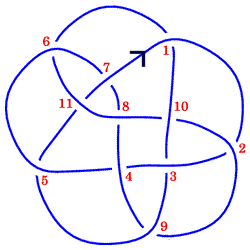
\includegraphics[width=0.65\linewidth]{../data/mixed/gauss_code.png}
        \subcaption{...dla kodu Gaußa}
    \end{minipage}
    \quad
    \begin{minipage}[b]{.45\linewidth}
        \centering
        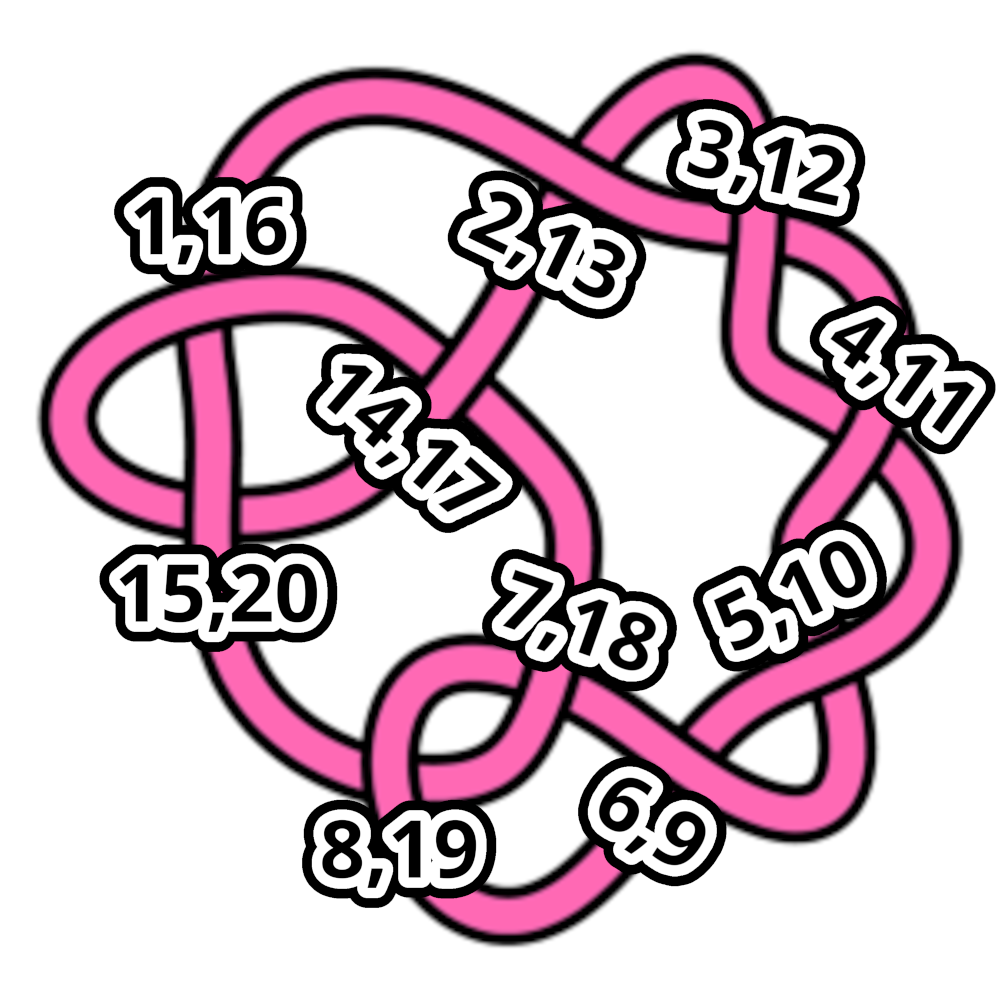
\includegraphics[width=0.65\linewidth]{../data/mixed/dowker_code.png}
        \subcaption{...dla kodu Dowkera-Thistlethwaite'a}
    \end{minipage}
    \caption[gauss-dowker-thistlethwaite]{Numeracja skrzyżowań}
    \label{gauss_dt}%
\end{figure}

% wiem o tym z "Aspects of topology, in memory of H. Dowker"
Gauß był świadomy, że szukanie koniecznych i wystarczających warunków na to, by ciąg $2n$ liczb był kodem jakiegoś węzła jest ciekawym problemem, ale chyba nie zdecydował się nim zająć.
Stosowne algorytmy podali trochę później topolodzy (Dehn \cite{dehn1936}) i dużo później teoretycy grafów (Rosenstiehl, Read \cite{rosenstiehl1978}).
Inny algorytm Dowkera, Thistlethwaite'a \cite{dowker1983} został zaimplementowany jako program komputerowy liczący około 30 linii kodu, stanowił ważny element tablicowania małych węzłów pierwszych.

\index{notacja!Gaußa|)}%

\subsubsection{Notacja Dowkera-Thistlethwaite'a}
\index{notacja!Taita}
\index{notacja!Dowkera-Thistlethwaite'a|(}
Poprawia nieopisaną tutaj notację Taita, opisana po raz pierwszy w~pracy \cite{dowker1983}.
\index[persons]{Dowker, Clifford}%
\index[persons]{Thistlethwaite, Morwen}%

Tak jak w~notacji Gaußa, przemierzamy węzeł zaczynając poza skrzyżowaniem.
Tym razem jednak stare skrzyżowania dostają drugi, nowy numer.
Jak można zauważyć, każde skrzyżowanie ma parzystą oraz nieparzystą etykietę.

\begin{definition}
    Ciąg parzystych liczb występujących na diagramie kolejno przy $1, 3, \ldots$ nazywamy kodem Dowkera-Thistlethwaite'a.
    Jeżeli nieparzysta etykieta odpowiadała podskrzyżowaniu, zapisujemy liczbę z~minusem.
\end{definition}

Opisany powyżej kod nie jest idealny, ponieważ odtworzony z niego węzeł może być lustrzanym odbiciem wyjściowego.
Ogólniej, odbicie dowolnego składnika sumy spójnej nie zmienia kodu całego węzła.
Nie stanowi to jednak dużego problemu, ponieważ notacja została stworzona na potrzeby tablicowania węzłów pierwszych, a~te są niezorientowane.

\begin{example}
    Rozpatrzmy węzeł z rysunku \ref{gauss_dt}.
    Jego kodem Dowkera-Thistlethwaite'a jest ciąg {16 12 10 18 6 4 2 20 14 8}.
\end{example}

Zaczynając od zredukowanego diagramu o $n$ skrzyżowaniach nie można doprowadzić do sytuacji, gdzie do pewnego skrzyżowania przypisane są dwie kolejne liczby całkowite.
Dzięki temu problem można przetłumaczyć na język teorii grafów.
Rozpatrzmy graf $G$, którego wierzchołkami są liczby $1, 2, \ldots, 2n$.
Połączmy niesąsiadujące modulo $2n$ wierzchołki o różnej parzystości krawędziami.
Graf ten powstaje przez usunięcie cyklu Hamiltona (łączącego kolejne liczby) z pełnego grafu dwudzielnego.
Zbiór par etykiet przy skrzyżowaniach węzła to skojarzenie doskonałe w grafie $G$.
Liczba skojarzeń prawie pokrywa się z rozwiązaniem zadania znanego w literaturze jako ,,\textsc{problème des ménages}'': na ile sposobów $n$ małżeństw można posadzić przy okrągłym stole tak, by żadne małżeństwo nie siedziało obok siebie i~każdy mężczyzna znalazł się obok dwóch kobiet?
\index{problem małżeństw przy stole}%
Ustawienia, które powstają przez cykliczne permutowanie należy uznać za tożsame.
Gilbert \cite{gilbert1956} znalazł wzór na $a_n$, liczbę różnych kodów:
\index[persons]{Gilbert, Edgar}%
\begin{align}
u(m, t) & = 2m \sum_{k=0}^m {2m-k \choose k} \cdot (m-k)! \cdot \frac{(t-1)^k}{2m - k}  \\
a(n) & = \frac{1}{n} \sum_{d\mid n} \left(\frac{n}{d}\right)^d \cdot u \left(d, 1 - \frac{d}{n}\right) \cdot \varphi \left(\frac{n}{d}\right)
\end{align}

Kilka początkowych wartości to $a_3 = 1, 2, 5, 20, 87, 616, 4843, 44128, 444621, \ldots$ (ciąg \href{https://oeis.org/A002484}{A002484} w OEIS).

\index{notacja!Dowkera-Thistlethwaite'a|)}%

\subsubsection{Notacja Alexandera-Briggsa}
\label{alexander_briggs_notation}%
\index{notacja!Alexandera-Briggsa|(}%
W~1927 roku Alexander, Briggs wprowadzili zupełnie inny sposób oznaczania węzłów -- wtedy do 9 skrzyżowań, ale przedłużony do 10 skrzyżowań przez Rolfsena i używany po dziś dzień.
Do opisu węzła używa się dwóch liczb: jego indeksu skrzyżowaniowanego z dolnym indeksem, oznaczającym miejsce w tablicy~węzłów.
I~tak węzły o~ośmiu skrzyżowaniach to $8_1, 8_2, \ldots,$ $8_{21}$.
Porządek jest umowny i jego wybór należy do osoby, która jako pierwsza znajdzie wszystkie węzły o danej liczbie skrzyżowań (ale węzeł skręcony występuje zawsze po torusowym).
% TODO: dlaczego?
\index{węzeł!skręcony}%
\index{węzeł!torusowy}%

Od jedenastu skrzyżowań pojawia się mała zmiana: węzły alternujące i niealternujące kataloguje się osobno.
I tak $11n_{185}$ to sto osiemdziesiąty piąty węzeł niealternujący o 11 skrzyżowaniach, zaś $11a_{367}$ to trzysta sześćdziesiąty siódmy alternujący.

Rolfsen w 1976 stworzył z kilkoma błędami tablicę diagramów pierwszych węzłów do 10 skrzyżowań.
\index[persons]{Rolfsen, Dale}%
\label{rolfsens_mistake}%
Para Perko $10_{161}, 10_{162}$ przedstawia ten sam węzeł, zaś górne skrzyżowanie w~$10_{144}$ powinno być zmienione.
\index{para Perko}%
Ostatnie cztery węzły dostały nowe numery, by uniknąć duplikatu.
Kolejną usterką tablicy jest to, że notacja Conwaya oraz wielomian Alexandera dla węzłów $10_{83}$ oraz $10_{86}$ są zamienione miejscami.
Tu czyha pułapka:\footnote{Wiemy o niej dzięki stronie \url{http://stoimenov.net/stoimeno/homepage/ptab/}.} Stojmenow, nowe wydanie książki Rolfsena, atlas węzłów Bar-Natana oraz tablica niezmienników węzłowych Livingstona naprawiają to przez wymianę podpisów.
Podręcznik Kawauchiego wymienia diagramy.

Ze strony internetowej Stojmenowa dowiedzieliśmy się jeszcze czegoś.
Kolejność Rolfsena dla węzłów o 10 skrzyżowaniach obala nomenklaturę Little'a niealternujących oraz nadpisuje numerowanie Taita dla alternujących węzłów.
\index[persons]{Little, Charles}%
Alexander, Briggs zrobili wcześniej to samo dla 9 lub mniej skrzyżowań.

\index{notacja!Alexandera-Briggsa|)}%

\subsubsection{Notacja Conwaya}
\index{notacja!Conwaya}%
Wprowadzona przez Conwaya w~pracy \cite{conway1970}.
Wymaga znajomości supłów, więc przedstawiamy ją po ich zdefiniowaniu, na stronie \pageref{conway_notation}.

\subsubsection{Nazwy zwyczajowe}
\label{sssec:link_names}%
Niektóre węzły i sploty, w szczególności te o niskim indeksie skrzyżowaniowym, występują tak często w teorii węzłów, że doczekały się nazw zwyczajowych.
Oto ich lista:
\begin{compactitem}
% DICTIONARY;unknot;niewęzeł;-
% TODO: nigdzie w książce nie ma definicji niesplotu?
    \item węzeł $0_1$ to niewęzeł;
\index{niewęzeł}%
% DICTIONARY;trefoil knot;trójlistnik;-
    \item węzeł $3_1$ to trójlistnik,
\index{trójlistnik}%
% DICTIONARY;figure-eight;ósemka;-
    \item węzeł $4_1$ to ósemka albo węzeł Listinga,
\index{ósemka}%
% DICTIONARY;cinquefoil knot;pięciolistnik;-
    \item węzeł $5_1$ to pięciolistnik albo węzeł Solomona (!),
\index{pięciolistnik}%
\index{węzeł Solomona}%
% DICTIONARY;stevedore knot;węzeł dokerski;-
    \item węzeł $6_1$ to węzeł dokerski/sztauerski,
\index{węzeł dokerski}%
    \item węzeł 11n34 to węzeł Conwaya,
\index{węzeł Conwaya}%
    \item węzeł 11n42 to węzeł Kinoshity-Terasakiego,
\index{węzeł Kinoshity-Terasakiego}%
    \item węzeł 12n242, czyli $(-2, 3, 7)$-precel, to z powodu pracy \cite{fintushel1980} węzeł  Fintushela-Sterna,
\index{węzeł Fintushela-Sterna}%
\index[persons]{Fintushel, Robert}%
\index[persons]{Stern, Robert}%
% DICTIONARY;granny knot;węzeł babski;-
    \item suma spójna takich samych trójlistników to węzeł babski,
\index{węzeł babski}
% DICTIONARY;square knot;węzeł prosty/płaski
    \item suma spójna lustrzanych trójlistników to, dość niefortunnie, węzeł prosty/płaski % (dość niefortunna nazwa),
% TODO: nigdzie w ksiażce nie ma definicji notacji A-B dla splotów?
    \item splot $2_1^2$ (L2a1) to splot Hopfa,
\index{splot Hopfa}%
    \item splot $4_1^2$ (L4a1) to węzeł Solomona (!),
\index{węzeł Solomona}%
    \item splot $5_1^2$ (L5a1) to splot Whiteheada,
\index{splot Whiteheada}%
    \item splot $6_2^3$ (L6a4) to pierścienie Boromeuszy.
\index{pierścienie Boromeuszy}%
\end{compactitem}




\section{Wykrywanie niewęzła}
Jednym z pierwszych dużych problemów teorii węzłów było poszukiwanie odpowiedzi na pytanie, kiedy diagram przedstawia niewęzeł.
\index{niewęzeł}%
Stosowny algorytm wykrywający niewęzły podał Haken \cite{haken1961}, ale długo nikt nie podjął się jego implementacji.
\index[persons]{Haken, Wolfgang}%
Epple pisze \emph{,,this algorithm was extremely impractical''}, w recenzji z MathSciNet proponuje, żeby przed przeczytaniem pełnej niepotrzebnych dygresji pracy Hakena poznać artykuł \cite{schubert1961} Schuberta.
\index[persons]{Epple, Moritz}%
\index[persons]{Schubert, Horst}%
W życie pomysły Hakena udało się wdrożyć Burtonowi, Budneyowi oraz Petterssonowi w~komputerowym programie Regina\footnote{\url{https://regina-normal.github.io/}.} na przełomie tysiącleci.

\index[persons]{Burton, Benjamin}%
\index[persons]{Budney, Ryan}%
\index[persons]{Pettersson, William}%
%=% https://mathscinet.ams.org/mathscinet-getitem?mr=141107
% DICTIONARY;incompressible;nieściśliwy;-

Burton, Rubinstein i~Tillman \cite{burton2012} pokazali, jak sprawdzać, w~czasie wykładniczym czy powierzchnia normalna na striangulowanej 3-rozmaitości jest (nie)ściśliwa.
\index[persons]{Rubinstein, Joachim}%
\index[persons]{Tillman, Stephan}%
To wystarczyło do udzielenia negatywnej odpowiedzi na pytanie Thurstona: \emph{,,czy przestrzeń Seiferta-Webera jest rozmaitością Hakena?''}, a zatem wykraczającego poza poziom naszego skromnego dzieła.
\index[persons]{Thurston, William}%
\index{przestrzeń!Seiferta-Webera}%
\index{rozmaitość!Hakena}%
(Rozmaitość Hakena to zwarta, $P^2$-nierozkładalna 3-rozmaitość, która jest dostatecznie duża, to znaczy zawiera właściwie zanurzoną dwustronną powierzchnię nieściśliwą, co za miks mądrych słów. Przykłady obejmują zwarte, nierozkładalne 3-rozmaitości z dodatnią pierwszą liczbą Bettiego, w tym wiązki powierzchniowe nad okręgiem; ale też dopełnienia splotów).

SnapPea\footnote{\url{http://geometrygames.org/SnapPea/index.html}.} to inny popularny wśród niskowymiarowych topologów program pozwalający badać hiperboliczne 3-rozmaitości, patrz sekcja \ref{sec:hyperbolic}.

Wiadomo, że genus oraz zredukowana kohomologia Chowanowa wykrywa niewęzły (fakty \ref{prp:genus_detects_unknot}, \ref{khovanov_detects_unknot}) i nie wiadomo, czy wielomian Jonesa to robi (hipoteza \ref{con:jones}).
\index{genus}%
\index{homologia!Chowanowa}%
\index{wielomian!Jonesa}%
Od dawna wiadomo, że wielomian Alexandera nie wykrywa niewęzła (fakt \ref{alexander_no_detects_unknot}).
\index{wielomian!Alexandera}%
W lutym 2021 Lackenby ogłosił nowy algorytm rozpoznający niewęzły w~quasiwielomianowym czasie.
% i nie zrobił tego w THE EFFICIENT CERTIFICATION OF KNOTTEDNESS AND THURSTON NORM, bo to wyszło na arxiv w 2016
\index[persons]{Lackenby, Marc}%

Wyśmienitym punktem wyjścia do poszukiwań trudnych niewęzłów jest praca \cite{schleimer2021}, dzieło Burtona, Changa, Löfflera, de Mesmaya, Marii, Schleimera, Sedgwicka oraz Spreera.
\index[persons]{Burton, Benjamin}%
\index[persons]{Chang, Hsien-Chih}%
\index[persons]{Mesmay, Arnaud@de Mesmay, Arnaud}%
\index[persons]{Löffler, Maarten}%
\index[persons]{Maria, Clément}%
\index[persons]{Schleimer, Saul}%
\index[persons]{Sedgwick, Eric}%
\index[persons]{Spreer, Jonatha}%
Cytuje ona artykuł Lackenby'a \cite{lackenby2015}, gdzie poznaliśmy stary (z 1934 roku!) przykład Goeritza \cite{goeritz1934} diagramu niewęzła o~11 skrzyżowaniach, który można zmienić w~zwykły diagram niewęzła tylko zwiększając po drodze liczbę skrzyżowań.
% 9781470454999 s. 5
\index[persons]{Goeritz, Lebrecht}%
\index{niewęzeł!Goeritza}%
Na kolejne teksty przyszło poczekać ponad pół wieku.
Autorzy przywołują jeszcze klasyczny przykład Freedmana, He, Wanga \cite{freedman1994}; ale też podstępne niewęzły Hakena, Ochiai, Thistlethwaite'a oraz mocno doświadczalną pracę Petronio, Zanellatiego \cite{zanellati2016}.
\index[persons]{Freedman, Michael}%
\index[persons]{He, Zheng-Xu}%
\index[persons]{Wang, Zhenghan}%
\index{niewęzeł!Freedmana}%
\index[persons]{Petronio, Carlo}%
\index[persons]{Zanellati, Adolfo}%

% TODO: sprawdzić, czy w \cite{heinrich2014} nie ma więcej trudnych niewęzłów

My nie potrafimy albo nie chcemy potrafić ładnie rysować, więc pozwolimy sobie pokazać tylko, jak wyglądał wspomniany wcześniej przykład Goeritza.
Na swoim blogu\footnote{\url{https://mickburton.co.uk/2015/06/05/how-do-you-construct-hakens-gordian-knot/}} Burton (inny Burton niż w poprzednim akapicie!) zamieścił wpis pełen rysunków, które tłumaczą, jak powstał niewęzeł Hakena.

\begin{comment}
\begin{figure}[H]
    \centering
    \begin{tikzpicture}[baseline=-0.65ex, scale=0.08]
        \begin{knot}[clip width=5, end tolerance=1pt, flip crossing/.list={1,2,3,4,8,9}]
            % horizontal lines
            \strand[ultra thick] (-40, -10) to (-10, -10);
            \strand[ultra thick] (-40, 10) to (-10, 10);
            \strand[ultra thick] (10, 10) to (30, 10);
            \strand[ultra thick] (10, -10) to (30, -10);
            % 
            \strand[ultra thick] (5-45, -10) [in=left,out=left] to (5-45, 3.33);
            \strand[ultra thick] (5-45, 10) [in=left,out=left] to (5-45, -3.33);
            \strand[ultra thick] (-5-35, -3.33) [in=left,out=right] to (5-35, 3.33);
            \strand[ultra thick] (-5-35, 3.33) [in=left,out=right] to (5-35, -3.33);
            \strand[ultra thick] (-5-25, -3.33) [in=left,out=right] to (5-25, 3.33);
            \strand[ultra thick] (-5-25, 3.33) [in=left,out=right] to (5-25, -3.33);
            \strand[ultra thick] (-5-15, -3.33) [in=left,out=right] to (5-15, 3.33);
            \strand[ultra thick] (-5-15, 3.33) [in=left,out=right] to (5-15, -3.33);
            %
            \strand[ultra thick] (-5+15, -3.33) [in=left,out=right] to (5+15, 3.33);
            \strand[ultra thick] (-5+15, 3.33) [in=left,out=right] to (5+15, -3.33);
            \strand[ultra thick] (-5+25, -3.33) [in=left,out=right] to (5+25, 3.33);
            \strand[ultra thick] (-5+25, 3.33) [in=left,out=right] to (5+25, -3.33);
            \strand[ultra thick] (-5+35, -3.33) [in=right,out=right] to (-5+35, 10);
            \strand[ultra thick] (-5+35, 3.33) [in=right,out=right] to (-5+35, -10);
            %
            \strand[ultra thick] (-5+5, 3.33) [in=left,out=right] to (5+5, 10);
            \strand[ultra thick] (-5+5, 10) [in=left,out=right] to (5+5, 3.33);
            \strand[ultra thick] (-5-5, 3.33) [in=left,out=right] to (5-5, 10);
            \strand[ultra thick] (-5-5, 10) [in=left,out=right] to (5-5, 3.33);
            %
            \strand[ultra thick] (-5+5, -10) [in=left,out=right] to (5+5, -3.33);
            \strand[ultra thick] (-5+5, -3.33) [in=left,out=right] to (5+5, -10);
            \strand[ultra thick] (-5-5, -10) [in=left,out=right] to (5-5, -3.33);
            \strand[ultra thick] (-5-5, -3.33) [in=left,out=right] to (5-5, -10);
        \end{knot}
    \end{tikzpicture}
    \caption{niewęzeł Goeritza}
\end{figure}
\end{comment}




\subsection{Hipotezy Taita}
\index{hipoteza!Taita|(}%

Tait na podstawie węzłów o małej liczbie skrzyżowań  wysunął około 1898 roku trzy lub cztery hipotezy.
Nie jest jasne, czy chodziło mu o wszystkie węzły, czy tylko te alternujące.
Uchylamy tutaj rąbka tajemnicy i~podajemy treść hipotez już teraz; dowód ze szczegółami odkładając na później, aż do sekcji \ref{sub:tait_conjectures}.
Tam też wspomnimy krótko o technikach użytych w dowodach pozostałych trzech.

\begin{conjecture}[I hipoteza Taita]
\index{indeks skrzyżowaniowy}%
\label{con:tait_1}%
    Zredukowany alternujący diagram splotu ma minimalny indeks skrzyżowaniowy.
\end{conjecture}

Najpierw znaleziono dowód korzystający z wielomianu Jonesa: dokonali tego w 1987 roku równocześnie Kauffman \cite{kauffman1987}, Murasugi \cite{murasugi1987} oraz Thistlethwaite \cite{thistlethwaite1987}.
\index[persons]{Kauffman, Louis}%
\index[persons]{Murasugi, Kunio}%
\index[persons]{Thistlethwaite, Morwen}%
Trzydzieści lat później Greene \cite{greene2017} zaprezentował geometryczne podejście do problemu.
\index[persons]{Greene, Joshua}%

\begin{conjecture}[II hipoteza Taita]
\index{spin}%
    Dwa zredukowane diagramy alternujące jednego węzła mają ten sam spin.
\end{conjecture}

Pierwsze dowody pochodzą znowu od Kauffmana \cite{kauffman1987} oraz Thistlethwaite'a \cite{thistlethwaite1987}.
\index[persons]{Kauffman, Louis}%
\index[persons]{Thistlethwaite, Morwen}%
Dla niektórych II hipoteza brzmi inaczej (,,achiralny splot alternujący ma zerowy spin''), dla innych jest prostym wnioskiem z naszego sformułowania.

\begin{conjecture}[III hipoteza Taita]
\index{flype}%
    Niech $D_1, D_2$ będą zredukowanymi alternującymi diagramami zorientowanego pierwszego splotu.
    Wtedy diagram $D_2$ można otrzymać z~$D_1$ korzystając jedynie z~ruchu \emph{flype}.
\end{conjecture}

Trzecią hipotezę udowodnił Menasco wspólnie z~Thistlethwaitem \cite{menasco1993}.
\index[persons]{Menasco, William}%
\index[persons]{Thistlethwaite, Morwen}%
Wynika z~niej, że dwa zredukowane diagramy alternujące tego samego węzła mają ten sam spin.
Nie jest prawdziwa dla niealternujących splotów, przez co w~tablicach węzłów tak długo mieliśmy duplikat -- parę Perko.
\index{para Perko}%

Czasami mówi się jeszcze o IV hipotezie: że zwierciadlane węzły mają parzysty indeks skrzyżowań.
\index{węzeł!zwierciadlany}
Ta okazała się fałszywa.

\index{hipoteza!Taita|)}%

% koniec podsekcji Hipotezy Taita





\chapter{Operacje węzłowe}

Mając dany diagram splotu zorientowanego, można odwrócić jego wszystkie ogniwa albo wszystkie skrzyżowania.
Działania te nazywamy odpowiednio rewersem i~lustrem, opisujemy je w~pierwszej podsekcji.
Dalej pojawi się suma niespójna oraz spójna, odpowiednik mnożenia liczb naturalnych zbadany dokładniej przez Schuberta około 1954 roku.
\index[persons]{Schubert, Horst}%
Znacznie później (bo dopiero w~sekcji \ref{sec:tangle}) wprowadzimy jeszcze sumę i~iloczyn supłów.


\section{Lustro i~rewers. Węzły skrętne i zwierciadlane}
\begin{definition}[lustro]
% DICTIONARY;mirror;lustro/lustrzany;węzeł
\index{lustro}%
\index{węzeł!lustrzany}% TODO: to się może mylić ze zwieciadlanym
    Niech $L$ będzie zorientowanym splotem.
    Splot $\operatorname{m} L$ powstały przez odbicie splotu $L$ względem dowolnej płaszczyzny nazywamy lustrem.
\end{definition}

\begin{definition}[rewers]
% DICTIONARY;reverse;rewers/odwrotny;węzeł
\index{rewers}%
\index{węzeł!odwrotny}%
    Niech $L$ będzie zorientowanym splotem.
    Splot $\operatorname{r} L$ powstały przez odwrócenie orientacji wszystkich ogniw splotu $L$ nazywamy rewersem.
\end{definition}

\begin{comment}
{\setlength{\intextsep}{4pt plus 2pt minus 2pt}
\begin{figure}[H]
    \begin{minipage}[b]{.32\linewidth}
        \centering
        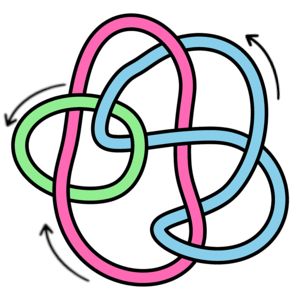
\includegraphics[height=2.2cm]{../data/links/9_3_2_mirror.png}
        \subcaption{lustro $mL$}
    \end{minipage}
    \begin{minipage}[b]{.32\linewidth}
        \centering
        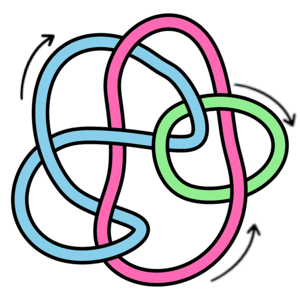
\includegraphics[height=2.2cm]{../data/links/9_3_2_base.png}
        \subcaption{przykładowy splot $L$}
    \end{minipage}
    \begin{minipage}[b]{.32\linewidth}
        \centering
        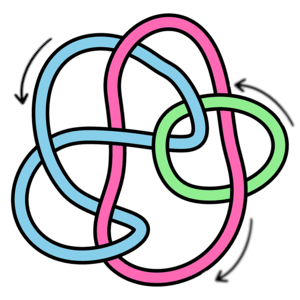
\includegraphics[height=2.2cm]{../data/links/9_3_2_reverse.png}
        \subcaption{rewers $rL$}
    \end{minipage}
\end{figure}
}
\end{comment}

Na lewym obrazku odbiliśmy diagram względem pionowej płaszczyzny, ale ten sam splot dostalibyśmy odwracając wszystkie nad- i podskrzyżowania (czyli odbijając go względem płaszczyzny papieru, ale programy graficzne nie pozwalają na wykonanie tej operacji zbyt łatwo, a~my jesteśmy trochę leniwi).

Niektórzy mówią o odbiciach lustrzanych i odwrotnościach.
Zaletą naszych oznaczeń jest to, że trudniej jest pomylić lustro z odwrotnością; ale w literaturze dominuje $L^*$ jako symbol lustra oraz $-L$ jako symbol odwrotności splotu $L$; używają ich na przykład Burde, Zieschang, Heusener \cite[s. 16]{burde2014} czy Murasugi \cite[s. 14, 24]{murasugi1996}.
Lickorish \cite[s. 4]{lickorish1997} używa $r L$ dla odwrotności oraz $\overline{L}$ dla lustra; zapewne ktoś gdzieś używa jeszcze innych znaczków.

Zauważmy, że wzięcie lustra i/lub rewersu węzła nie musi prowadzić do nowych obiektów.
Na przykład trójlistnik jest własnym rewersem: $3_1 = \operatorname{r} 3_1$, ale nie lustrem.

Dlatego wyróżniamy pięć typów symetrii splotów:

\begin{definition}[sploty zwierciadlane, odwracalne, chiralne]
% DICTIONARY;chiral;skrętny/chiralny;węzeł
% DICTIONARY;reversible;odwracalny;węzeł
% DICTIONARY;achiral/amphicheiral;zwierciadlany;węzeł
    Niech $L$ będzie splotem.
    Wtedy $L$ jest równoważny ze swoim rewersem, lustrem, rewersem lustra, wszystkimi albo żadnym z trzech wymienionych splotów;
    splot $L$ nazywamy odpowiednio:
    \begin{itemize}
        \item odwracalnym ($L = rL$),
        \item dodatnio zwierciadlanym ($L = mL$),
        \item ujemnie zwierciadlanym ($L = mrL$),
        \item całkowicie zwierciadlanym ($mL = L = rL$),
        \item całkowicie chiralnym ($mL \neq L \neq rL$).
    \end{itemize}
\index{węzeł!zwierciadlany}%
\index{węzeł!odwracalny}%
\index{węzeł!chiralny}%
\index{węzeł!skrętny|see {węzeł chiralny}}%
\end{definition}

Węzły całkowicie chiralne nazywa się czasem skrętnymi.

%    Węzły $K$, $rK$, $mK$ są parami nierównoważne. % chiral 9_32
%    Węzły $K \cong rK$ są równoważne. % reversible 3_1
%    Węzły $K \cong mrK$ są równoważne. % negative amphicheiral 8_17
%    Węzły $K \cong mK$ są równoważne. % positive amphicheiral 12a_427
%    Węzły $K, rK, mK$ są parami równoważne. % fully amphicheiral 4_1

\begin{example}
    Węzeł $9_{32}$ jest całkowicie skrętny.
\end{example}

% Całkowicie skrętne są też między innymi wszystkie węzły torusowe.
% TODO: wiki pisze Each nontrivial torus knot is prime[4] and chiral.[2]

\begin{example}
    \label{exm:trefoil_is_chiral}
    Trójlistnik jest odwracalny, ale nie zwierciadlany.
\end{example}

Przypuszczał to już Listing \cite{listing1847} w 1847 roku, ale pierwszy dowód podał dużo później, bo w 1914 roku Dehn \cite{dehn1914}. 
Oto, jak tego dokonał.
% równik = equator
% równoleżnik = parallel (of latitude), najdłuższy równoleżnik to równik
% południk = meridian (of longitude)
% TODO: meridian pojawia się u Burdego, Zieschanga na s. 21 (2013) (numeracja papierowa)
% TODO: naprostować bałagan z meridian/longitude w całej książce
% https://math.stackexchange.com/questions/2511364/how-did-dehn-prove-that-the-trefoil-is-chiral myli te pojęcia: pisze o meridian i longitude, kiedy oryginalna praca Dehna operowała na longitude i latitude
\begin{proof}[Niedowód]
    Iloraz grafu Cayleya dla grupy podstawowej trójlistnika, $G = \pi_1(S^3 - K)$, zanurza się w~produkt $\mathbb H^2 \times \R$, co pozwala wyznaczyć grupę zewnętrznych automorfizmów grupy $G$, $\Z/2\Z$.
\index{grupa!podstawowa}
% DICTIONARY;latitude;szerokość geograficzna;geografia
% DICTIONARY;longitude;długość geograficzna;geografia
% DICTIONARY;meridian (of longitude);południk;geografia
% DICTIONARY;parallel (of latitude);równoleżnik;geografia
% DICTIONARY;---;geografia;-
Korzystając z~południków i~równoleżników pokazał następnie, że nietrywialny automorfizm zewnętrzny odwraca orientację przestrzeni otaczającej.
\end{proof}

My przekonamy się o~tym po wyznaczeniu wielomianu Jonesa trójlistnika (wniosek \ref{cor:jones_of_amphicheiral}).
Burde, Zieschang, Heusener \cite[s. 79]{burde2014} wyprowadzają ten sam wynik z~własności węzłów rozwłóknionych.

\begin{example}
    Węzeł $8_{17}$ jest zwierciadlany ujemnie, ale nie odwracalny.
\end{example}

Nieodwracalności $8_{17}$ dowiedli niezależnie około 1979 roku Kawauchi \cite{kawauchi1979} oraz Bonahon, Siebenmann \cite{bonahonf1979}.

Sześćdziesiąt lat temu matematycy nie byli pewni, czy węzły nieodwracalne w~ogóle istnieją \cite[problem 10]{fox1962};
obecnie wiadomo, że nieodwracalne są prawie wszystkie węzły (Murasugi \cite[s.~46]{murasugi1996}).
\index[persons]{Murasugi, Kunio}%
W~roku 1962 Ralph Fox wskazał kilku kandydatów do tego tytułu.
\index[persons]{Fox, Ralph}%
Hale Trotter odkrył rok później nieskończoną rodzinę nieodwracalnych precli, patrz \ref{prp:pretzel_not_invertible}.
\index[persons]{Trotter, Hale}%

% MAKOTO SAKUMA - A SURVEY OF THE IMPACT OF THURSTON’S WORK ON KNOT THEORY
% Hartley [129] realized that one can apply this method to the problem of identifying noninvertible knots, as follows. Suppose no automorphism of Γ maps γ to γ−1. Then the set R(G(K), Γ, γ) is possibly different from the set R(G(K), Γ, γ−1), and there is a chance to show noninvertibility of K by comparing the homology invariants associated with φ ∈ R(G(K), Γ, γ) with those associated with φ′ ∈ R(G(K), Γ, γ−1). Hartley showed that this method is quite effective: he completely determined the 36 non-invertible knots up to 10 crossings claimed by Conway to be noninvertible.

\begin{example}
    Węzeł $12a_{427}$ jest zwierciadlany dodatnio, ale nie odwracalny.
\end{example}

Żaden inny węzeł pierwszy o mniej niż 13 skrzyżowaniach nie ma tej cechy.

\begin{example}
\label{property_of_eight_knot}%
    Ósemka $4_1$ jest całkowicie zwierciadlana.
\end{example}

To najprostszy typ symetrii, wystarczy jawnie wskazać przekształcenie między diagramem węzła, jego lustra oraz odwrotności.

\label{con:tait_fourth}%
Tait odnosił wrażenie, że zwierciadlane węzły mają parzysty indeks skrzyżowań, ale Hoste, Thistlethwaite znaleźli w~1998 kontrprzykład o~piętnastu skrzyżowaniach, $15_{700}$. % wg https://mathworld.wolfram.com/AmphichiralKnot.html
(Czwarta) hipoteza Taita jest prawdziwa dla węzłów pierwszych, alternujących.
\index{hipoteza!Taita}%

Poniższa tabela oparta jest (kolejno) o~ciągi
\href{https://oeis.org/A051766}{51766},
\href{https://oeis.org/A051769}{51769},
\href{https://oeis.org/A051768}{51768},
\href{https://oeis.org/A051767}{51767},
\href{https://oeis.org/A052400}{52400},
z bazy danych ``The On-Line Encyclopedia of Integer Sequences'' (OEIS).

\begin{table}[h]
    \centering
    \begin{tabular}{@{}*{20}l@{}} \toprule
        skrzyżowania & 3 & 4 & 5 & 6 & 7 & 8 & 9 & 10 & 11 & 12 & 13 & 14 \\ \midrule
        całkowicie skrętne & 0 & 0 & 0 & 0 & 0 & 0 & 2 & 27 & 187 & 1103 & 6919 & 37885 \\
        odwracalne & 1 & 0 & 2 & 2 & 7 & 16 & 47 & 125 & 365 & 1015 & 3069 & 8813 \\
        $-$ zwierciadlane & 0 & 0 & 0 & 0 & 0 & 1 & 0 & 6 & 0 & 40 & 0 & 227 \\
        $+$ zwierciadlane & 0 & 0 & 0 & 0 & 0 & 0 & 0 & 0 & 0 & 1 & 0 & 6 \\
        zwierciadlane & 0 & 1 & 0 & 1 & 0 & 4 & 0 & 7 & 0 & 17 & 0 & 41 \\
        \bottomrule
        \hline
    \end{tabular}
    \caption{Liczba węzłów pierwszych o~poszczególnych typach symetrii}
\end{table}

\begin{definition}
    Niech $K \subseteq S^3$ będzie węzłem.
    Jeśli istnieje inwolucja pary $(S^3, K)$, która zachowuje orientację sfery, ale odwraca orientację węzła, to węzeł $K$ nazywamy silnie odwracalnym.
\end{definition}

To jest definicja 10.3.2 z monografii Kawauchiego \cite{kawauchi1996}.

\begin{proposition}
    Jeśli węzeł jest silnie odwracalny, to jest też odwracalny.
\end{proposition}

Hipotezę, że każdy odwracalny węzeł jest też silnie odwracalny, postawił Montesinos \cite[problem 1.6]{kirby1978}, on też zdefiniował klasę silnie odwracalnych węzłów \cite{montesinos1975}.
\index[persons]{Montesinos, José}%
Jednakże...

\begin{proposition}
    Istnieją odwracalne węzły, które nie są silnie odwracalne.
\end{proposition}

\begin{proof}
\index[persons]{Hartley, Richard}%
\index[persons]{Whitten, Wilbur}%
    Stosowne przykłady podali niezależnie od siebie Hartley \cite[s. 183]{hartley1980} oraz Whitten \cite{whitten1981} (węzeł $K$ jest silnie odwracalny wtedy i tylko wtedy, gdy każdy jego dubel jest silnie nieodwracalny, wynika stąd, że pewien dubel $8_{17}$ nie jest silnie odwracalny; jednocześnie Schubert \cite[s. 235]{schubert1953} pokazał, że duble są odwracalne).
\end{proof}

Ale hiperboliczny węzeł odwracalny jest silnie odwracalny, wspomina o tym bez dowodu Kawauchi.

\begin{proposition}
    Każdy wielomian Alexandera jest realizowany przez pewien silnie odwracalny węzeł.
\end{proposition}

\begin{proof}[Niedowód]
\index[persons]{Sakai, Tsuyoshi}%
    Sakai \cite{sakai1983} dla każdego cyklicznego modułu Alexandera $M$ skonstruował silnie odwracalny węzeł $K$, którego modułem Alexandera jest właśnie $M$.
\end{proof}

% Koniec podsekcji Lustro i rewers




\subsection{Węzły okresowe}
\index{węzeł!okresowy|(}%
Można wyróżnić jeszcze jeden rodzaj symetrii.

% DICTIONARY;period;okres;-
% DICTIONARY;periodic;okresowy;węzeł
\begin{definition}
\label{def:period}%
    Węzeł $K$ nazywamy $n$-okresowym, jeśli istnieje obrót $f \colon \R^3 \to \R^3$ o~kąt $2\pi/n$ wokół pewnej prostej $l$, rozłącznej z~węzłem $K$, taki że $f(K) = K$.
\end{definition}

Zamiast obrotów można rozpatrywać dowolne odwzorowania okresowe $f \colon S^3 \to S^3$, których zbiór punktów stałych jest rozłączny z węzłem $K$, homeomorficzny z $S^1$ oraz które trzymają węzeł $K$ w miejscu, ale dostaje się wtedy dokładnie taką samą klasę węzłów.
Czemu?
Wynika to z hipotezy Smitha, otrzymanej z połączenia głębokich teorii dotyczących geometrii i topologii 3-rozmaitości.
\index{hipoteza!Smitha}%
Kawauchi \cite[s. 125]{kawauchi1996} odsyła tu do książki Morgana, Bassa \cite{morgan1984}, gdzie znajdziemy problem, jego historię i rozwiązanie.
\index[persons]{Morgan, John}%
\index[persons]{Bass, Hyman}%

\begin{proposition}
    Zbiór wszystkich okresów jest niezmiennikiem węzłów.
\end{proposition}

Nieodwracalny węzeł $8_{17}$ nie posiada żadnych okresów.
% ćwiczenie 10.1.5 w Kawauchi
Węzeł $5_1$ jest 5-okresowy, co widać na standardowym diagramie, oraz 2-okresowy, tę drugą symetrię można dostrzec na diagramie realizującym liczbę mostową.
Trójlistnik ma dokładnie dwa okresy, $2$ i~$3$.
Ogólniej, jak głosi Kawauchi \cite[ćwiczenie 10.1.9]{kawauchi1996}:

\begin{proposition}
    Jedynymi okresami węzła $(p, q)$-torusowego są dzielniki liczb $p$ oraz $q$.
\end{proposition}

Murasugi podał dwa warunki, które musi spełniać węzeł o~okresie $n = p^r$, gdzie $r$ jest liczbą pierwszą.
Do ich zrozumienia potrzebujemy dwóch definicji.

\begin{definition}
    Niech $f$ będzie obrotem z definicji \ref{def:period}, zaś $p \colon \R^3 \to \R^3/f \simeq \R^3$ rzutem na przestrzeń ilorazową.
% DICTIONARY;quotient;ilorazowy;węzeł
\index{węzeł!ilorazowy}%
    Wtedy $p(K)$ nazywamy \emph{węzłem ilorazowym}, zaś $K$ to jego $n$-krotne nakrycie.    
\end{definition}

Ładny rysunek węzła ilorazowego znaleźliśmy u Kawauchiego \cite[s. 122]{kawauchi1996}.

\begin{definition}
    Niech $K$ będzie zorientowanym węzłem, zaś $l$ zorientowaną półprostą, która nie jest styczna do węzła $K$.
    Wtedy różnicę między liczbą skrzyżowań dodatnich oraz ujemnych wzdłuż półprostej (bez znaku) nazywamy indeksem zaczepienia $\lambda$ węzła $p(K)$.
\end{definition}

\begin{proposition}[warunek Murasugiego]
\index{warunek!Murasugiego}%
\label{prp:murasugi_periodic}%
    Niech $K$ będzie węzłem o~okresie $n = p^r$, gdzie $p$ jest liczbą pierwszą.
    Niech $J$ będzie jego węzłem ilorazowym, z~indeksem zaczepienia $\lambda$.
    Wtedy wielomian $\alexander_J$ jest dzielnikiem wielomianu $\alexander_K$ oraz istnieje pewna całkowita liczba $k$, taka że
    \begin{equation}
        \alexander_K(t) \equiv \pm t^k \alexander_J(n)^n \left(1 + t + t^2 + \ldots + t^{\lambda - 1}\right)^{n-1} \mod p.
    \end{equation}
\end{proposition}

\begin{proof}[Niedowód]
    Mozolne operacje na macierzach, których wyznacznikiem jest wielomian Alexandera, patrz \cite{murasugi1971}.
    Kawauchi przedstawia inny dowód: najpierw dowodzi tego dla węzła torusowego $T_{n, d}$, którego węzłem ilorazowym jest niewęzeł.
    W ogólnym przypadku, korzysta z relacji kłębiastej dla wielomianu Conwaya.
    Szczegóły oraz odsyłacze do dalszych prac znaleźć można w jego przeglądowej publikacji \cite[s. 122-124]{kawauchi1996}.
\end{proof}

Z prac Borodzika (m.in. \cite{grabowski20} napisanej z Grabowskim, Królem i Marchwicką) dowiedzieliśmy się, że podany wyżej warunek Murasugiego jest tylko jednym z wielu ograniczeń, jakie musi spełniać węzeł okresowy.
Autorzy wymieniają:
\begin{itemize}
    \item warunek Murasugiego udoskonalony przez Davisa, Livingstona \cite{davis1991},
\index[persons]{Davis, James}%
\index[persons]{Livingston, Charles}%
    \item kryterium Naika z homologiami rozgałęzionego nakrycia \cite{naik1997},
\index[persons]{Naik, Swatee}%
\index{homologie}%
\index{rozgałęzione nakrycie}%
    \item kryterium Traczyka z wielomianem Jonesa \cite{traczyk1991},
\index{wielomian Jonesa}%
\index[persons]{Traczyk, Paweł}%
    \item kryterium Przytyckiego z wielomianem HOMFLY-PT \cite{przytyckij1989},
\index{wielomian HOMFLY-PT}%
\index[persons]{Przytycki, Józef}%
    \item kryterium Naika z niezmiennikiem Cassona-Gordona,
\index{niezmiennik Cassona-Gordona}%
\index[persons]{Naik, Swatee}%
    \item kryterium Hillmana, Livingstona, Naika ze skręconym wielomianem Alexandera \cite{hillman2006},
\index{wielomian Alexandera!skręcony}%
\index[persons]{Hillman, Jonathan}%
\index[persons]{Livingston, Charles}%
\index[persons]{Naik, Swatee}%
    \item kryterium Jabuki, Naika z homologią Floera \cite{jabuka2016},
\index{homologia Floera}%
\index[persons]{Jabuka, Stanisław}%
\index[persons]{Naik, Swatee}%
    \item kryteria Borodzika, Politarczyka z homologią Chowanowa, \cite{politarczyk2017}, \cite{politarczyk2021},
\index{homologia Chowanowa}%
\index[persons]{Borodzik, Maciej}%
\index[persons]{Politarczyk, Wojciech}%
    \item kryterium Chena z grupą podstawową \cite{chen2018}.
\index{grupa podstawowa}%
\index[persons]{Chen, Haimiao}%
\end{itemize}
% Sakumy nie ma, bo nie został wymieniony ze słowem criterion; być może napisał coś ogólnego? 
\index{kryterium Naika (okresowości)}%

\index{węzeł!okresowy|)}%

% koniec podsekcji Węzły okresowe




\subsection{Suma niespójna i~suma spójna}

\begin{definition}[suma niespójna]
% DICTIONARY;distant union;suma niespójna;-
\index{suma niespójna}%
    Niech $L_1$ oraz $L_2$ będą splotami, które leżą po różnych stronach ustalonej płaszczyzny w przestrzeni $\R^3$.
    Teoriomnogościową sumę $L_1 \sqcup L_2$ nazywamy sumą niespójną splotów $L_1$ i $L_2$.
\end{definition}

\begin{definition}[suma spójna]
% DICTIONARY;connected sum;suma spójna;-
\index{suma spójna}%
\label{def:connected_sum}%
    Niech $K_1, K_2$ będą zorientowanymi węzłami.
    Natnijmy każdy z nich w dwóch punktach tego samego krótkiego łuku, a następnie zszyjmy dwoma łukami, które nie przecinają już istniejących, jak na obrazku.
    Otrzymany węzeł nazywamy sumą spójną węzłów $K_1$ oraz $K_2$ i oznaczamy przez $K_1 \shrap K_2$.
\begin{comment}
    \[
        \begin{tikzpicture}[baseline=-0.65ex,scale=0.09]
        \useasboundingbox (-12, -15) rectangle (12, 10);
        \begin{knot}[clip width=5, flip crossing/.list={5}, ignore endpoint intersections=false,]
            \strand[thick] (-3.5, -3.5) [in=down, out=up] to (3.5, 3.5);
            \strand[thick] (3.5, 3.5) [in=right, out=up] to (-4.5, 10);
            \strand[thick] (-4.5, 10) [in=up, out=left] to (-10, 3.5);
            \strand[thick] (-10, 3.5) to (-10, -3.5);
            \strand[thick] (-10, -3.5) [in=left, out=down] to (-4.5, -10);
            \strand[thick] (-4.5, -10) [in=down, out=right] to (3.5, -3.5);
            \strand[thick] (3.5, -3.5) [in=down, out=up] to (-3.5, 3.5);
            \strand[thick] (-3.5, 3.5) [in=left, out=up] to (4.5, 10);
            \strand[thick] (4.5, 10) [in=up, out=right] to (10, 3.5);
            \strand[thick, -Latex] (10, 3.5) to (10, -3.5);
            \strand[thick] (10, -3.5) [in=right, out=down] to (4.5, -10);
            \strand[thick] (4.5, -10) [in=down, out=left] to (-3.5, -3.5);
            \node at (0, -15) {$K_1$};
        \end{knot}
        \end{tikzpicture}
        \shrap
        \begin{tikzpicture}[baseline=-0.65ex,scale=0.09]
        \useasboundingbox (-12, -15) rectangle (12, 10);
        \begin{knot}[clip width=5, flip crossing/.list={6}, ignore endpoint intersections=false,]
            \strand[thick] (-3.5, -3.5) [in=down, out=up] to (3.5, 3.5);
            %\strand[thick] (3.5, 3.5) [in=right, out=up] to (-4.5, 10);
            %\strand[thick] (-4.5, 10) [in=up, out=left] to (-10, 3.5);
            \strand[thick] (-10, -3.5) [in=left, out=up] to (0, 6.5);
            \strand[thick, Latex-] (-10, -3.5) [in=left, out=down] to (-4.5, -10);
            \strand[thick] (-4.5, -10) [in=down, out=right] to (3.5, -3.5);
            \strand[thick] (3.5, -3.5) [in=down, out=up] to (-3.5, 3.5);
            %\strand[thick] (-3.5, 3.5) [in=left, out=up] to (4.5, 10);
            %\strand[thick] (4.5, 10) [in=up, out=right] to (10, 3.5);
            \strand[thick] (10, -3.5) [in=right, out=up] to (0, 6.5);
            \strand[thick] (10, -3.5) [in=right, out=down] to (4.5, -10);
            \strand[thick] (4.5, -10) [in=down, out=left] to (-3.5, -3.5);
            %
            \strand[thick] (-3.5, 3.5) [in=left, out=up] to (0, 10);
            \strand[thick] (3.5, 3.5) [in=right, out=up] to (0, 10);
            \node at (0, -15) {$K_2$};
        \end{knot}
        \end{tikzpicture}
        =
        \begin{tikzpicture}[baseline=-0.65ex,scale=0.09]
        \useasboundingbox (-27, -15) rectangle (27, 10);
        \begin{knot}[clip width=5, flip crossing/.list={5, 22, 23}, ignore endpoint intersections=false,]
            \strand[thick] (-18.5, -3.5) [in=down, out=up] to (-11.5, 3.5);
            \strand[thick] (-11.5, 3.5) [in=right, out=up] to (-19.5, 10);
            \strand[thick] (-19.5, 10) [in=up, out=left] to (-25, 3.5);
            \strand[thick] (-25, 3.5) to (-25, -3.5);
            \strand[thick] (-25, -3.5) [in=left, out=down] to (-19.5, -10);
            \strand[thick] (-19.5, -10) [in=down, out=right] to (-11.5, -3.5);
            \strand[thick] (-11.5, -3.5) [in=down, out=up] to (-18.5, 3.5);
            \strand[thick] (-18.5, 3.5) [in=left, out=up] to (-10.5, 10);
            \strand[thick] (-10.5, 10) [in=left, out=right] to (-5, 2);
            \strand[thick, -Latex] (-5, 2) to (-5+6, 2);
            \strand[thick] (5, 2) to (-5+6, 2);
            \strand[thick] (3, -2) to [in=left, out=right] (10.5, -10);
            \strand[thick, -Latex] (3, -2) to (-3, -2);
            \strand[thick] (-5, -2) to (-3, -2);
            \strand[thick] (-5, -2) [in=right, out=left] to (-10.5, -10);
            \strand[thick] (-10.5, -10) [in=down, out=left] to (-18.5, -3.5);
            %%%
            \strand[thick] (11.5, -3.5) [in=down, out=up] to (18.5, 3.5);
            \strand[thick] (-10 +15, 2) [in=left, out=right] to (15, 6.5);
            \strand[thick] (10.5, -10) [in=down, out=right] to (18.5, -3.5);
            \strand[thick] (18.5, -3.5) [in=down, out=up] to (11.5, 3.5);
            \strand[thick] (25, -3.5) [in=right, out=up] to (15, 6.5);
            \strand[thick] (25, -3.5) [in=right, out=down] to (19.5, -10);
            \strand[thick] (19.5, -10) [in=down, out=left] to (11.5, -3.5);
            \strand[thick] (11.5, 3.5) [in=left, out=up] to (15, 10);
            \strand[thick] (18.5, 3.5) [in=right, out=up] to (15, 10);
            %%%
            \node at (0, -15) {$K_1 \shrap K_2$};
        \end{knot}
        \end{tikzpicture}
    \]
\end{comment}
\end{definition}

W topologii rozważa się podobną operację: z~każdej $n$-rozmaitości wycina się kulę, po czym skleja wzdłuż brzegowej sfery w~jedną rozmaitość.
Ale kiedy zajmujemy się węzłami, nie interesuje nas struktura rozmaitości (gdyż każdy węzeł jest homeomorficzny z~okręgiem), tylko zanurzenie w otaczającą przestrzeń.
Pojęcie sumy spójnej węzłów (oraz opisane później satelity) wprowadził do matematyki Schubert \cite{schubert1949}.
\index[persons]{Schubert, Horst}%

Żadnego elementu definicji \ref{def:connected_sum} nie można pominąć:
\begin{itemize}
    \item \emph{składniki $K_1, K_2$ muszą być zorientowane}. 
    Węzeł prosty, czyli suma dwóch przeciwnie skręconych trójlistników, ma zerową sygnaturę i jest plastrowy.
    \index{węzeł!plastrowy}%
    \index{sygnatura}%
    Węzeł babski, czyli suma tak samo skręconych trójlistników ma niezerową sygnaturę.
    (To jedno z niewielu miejsc, gdzie nomenklatura pochodzi od żeglarzy.).
    \label{two_sums_of_two_trefoils}%
    Uzasadnienie, że te węzły są różne, nie jest łatwym zadaniem.
    Fox twierdzi, że Seifert \cite{seifert1933} wiedział o tym.
    Pokazał też w~króciutkim artykule \cite{fox1952}, że ich dopełnienia nie są homeomorficzne.
    \item \emph{składniki $K_1, K_2$ muszą być węzłami, nie splotami}. Nie istnieje kanoniczny wybór, które ogniwa łączyć ze sobą.
    \item \emph{zszywajace łuki nie mogą przecinać diagramów}.
    Cromwell \cite[s. 90]{cromwell2004} pokazuje przykład dwóch niewęzłów, z~których otrzymano niepoprawnie dwie różne sumy, $6_1$ oraz $8_{20}$.
\end{itemize}

\begin{proposition}
    Suma spójna węzłów jest dobrze określonym działaniem.
    Jest łączna i przemienna; niewęzeł stanowi jej element neutralny.
\end{proposition}

\begin{proof}
    Niech dane będą węzły $K_1$ oraz $K_2$ oraz dwa różne łuki $\gamma_1$, $\gamma_2$, których można użyć do konstrukcji sumy spójnej.
    Skurczmy $K_1$ tak, by był bardzo mały, przeciągnijmy najpierw przez łuk $\gamma_1$, a~następnie wzdłuż węzła $K_2$ do miejsca, gdzie zaczyna się łuk $\gamma_2$.
    Na koniec odwróćmy proces, z łukiem~$\gamma_2$ w~miejscu łuku $\gamma_1$.

    Prosty dowód drugiego zdania pozostawiamy Czytelnikowi.
\end{proof}

Algebra powiedziałaby, że węzły z~sumą spójną tworzą półgrupę, podobnie jak liczby naturalne z~działaniem dodawania.
Do bycia grupą brakuje istnienia elementów przeciwnych. 
Znane są nam co najmniej trzy różne sposoby na uzasadnienie tego faktu.

Najpierw wywnioskowaliśmy to z~własności powierzchni Seiferta i~ich genusu: faktów \ref{prp:genus_detects_unknot} oraz \ref{prp:genus_of_sum}.
O~tym samym dowodzie wspomina Kawauchi \cite[s. 33]{kawauchi1996}, a~fakt nazywa twierdzeniem o~nieanulowaniu.
Potem poznaliśmy szwindel Mazura, technikę dowodzenia bardziej przystępną dla kogoś, kto nie zna topologii algebraicznej, ale niestety wykorzystującą węzły dziki.
Długo myśleliśmy, że inaczej się nie da, ale elementarny dowód istnieje!
% odkryte w https://aperiodical.com/2018/07/the-big-internet-math-off-round-1-jim-propp-v-zoe-griffiths/
Trzeba zajrzeć do \cite[s. 18-20]{kauffman1995} dla dwóch rysunków tamże.

\begin{proposition}
\label{first_time_sum_is_trivial}%
    Niech $K_1, K_2$ będą takimi węzłami, że $K_1 \shrap K_2 = \SmallUnknot$. Wtedy $K_1 = K_2 = \SmallUnknot$.
\end{proposition}

\begin{proof}[Niedowód]
% DICTIONARY;Mazur swindle;szwindel Mazura;-
    Technika ta zwana jest szwindlem Mazura.
\index{szwindel Mazura}%
    Załóżmy, że $K \shrap L = \SmallUnknot$ i~dopuśćmy wyjątkowo węzły dzikie.
    Skonstruujmy sumę $K \shrap L \shrap K \shrap \ldots$,
    przy czym kolejne składniki powinny zmniejszać się,
    aby ich suma nadal była węzłem.
    Wtedy
    \begin{align*}
        K & \simeq K \shrap [(L \shrap K) \shrap (L \shrap K) \ldots] \\
         & \simeq (K \shrap L) \shrap (K \shrap L) \shrap \ldots
         \simeq \SmallUnknot \shrap \SmallUnknot \shrap \ldots
         \simeq \SmallUnknot.
    \end{align*}
    Analogicznie pokazujemy, że $L \simeq \SmallUnknot$.
    (To jedyne miejsce w~całej książce, gdzie użyte zostają węzły dzikie.)
\end{proof}

\begin{proof}
    (Na podstawie \cite[s. 18-20]{kauffman1995}).
    Wyobraźmy sobie, że węzeł oraz torus połykająco-podążający $T$ został zawieszony między dwiema ścianami pokoju i~załóżmy nie wprost, że suma $K = K_1 \shrap K_2$ jest trywialna.
    Wtedy pewien homeomorfizm pokoju, który nie rusza ścian, prostuje sumę (zamienia pozornie zaplątany węzeł $K$ w odcinek $L$). 

    Niech $\pi$ będzie dowolną płaszczyzną zawierającą wyprostowaną sumę $K$.
    Tnie część wspólną torusa $T$ oraz ścian w czterech punktach, oznaczmy je $A, B$ (na lewej ścianie) oraz $C, D$ (na prawej).
    Zauważmy, że $\pi$ tnie $T$ w łukach, które wychodzą z $A, B, C, D$ oraz pewnych zamkniętych krzywych.
    Łuk wychodzący z~punktu $A$ nie może łączyć go z punktami $B$ lub $D$, ponieważ te leżą po drugiej stronie odcinka $L$ na płaszczyźnie $\pi$.
    
    Łuk $AC$ przedstawia niewęzeł.
    Jednocześnie jest on obrazem pewnego łuku, który łączył końce torusa $T$, zatem musi być równoważny z~węzłem-towarzyszem.
\end{proof}

Półgrupę węzłów z~operacją sumy spójnej można uczynić grupą na dwa sposoby: albo zmieniając działanie, albo osłabiając równoważność węzłów.
Drugi pomysł jest lepszy niż pierwszy.
Na początku lat pięćdziesiątych Milnor wprowadził pojęcie zgodności.
\index{węzeł!plastrowy}%
\index{węzeł!zgodny}%
Element neutralny nowej grupy to węzły plastrowe, ich opis leży w~sekcji \ref{sec:slice}.
Zgodność i plastrowe węzły to zagadnienia zakorzenione w~czterowymiarowej topologii.

Kawauchi \cite[s. 50-53]{kawauchi1996} opisuje $2n$-sumę Murasugiego tak, że $2$-suma to nasza suma spójna, zaś $4$-suma to \textsc{,,plumbing''} (coś, czego nie znamy) i dodaje komentarz, że jest bardzo przydatna do badania powierzchni Seiferta czy genusu.
\index{plumbing}%
\index{suma Murasugiego}%
Została wprowadzona dawno temu w~\cite{murasugi1958}, by szacować stopień wielomianu Alexandera alternujących węzłów.
\index[persons]{Murasugi, Kunio}%
\index{wielomian Alexandera}%
\index{sploty alternujące}%

% DICTIONARY;suma paskowa;band sum;-
Innym uogólnieniem jest suma paskowa, patrz \cite[s. 31-32, 43]{kawauchi1996}, specjalny przypadek hiperbolicznej transformacji splotu oraz fuzji splotu.
\index{suma paskowa}%
% TODO: sprawdzić, czy fuzja splotu ma trafić do indeksu

% Koniec podsekcji Suma niespójna i suma spójna





% DICTIONARY;prime;pierwszy;węzeł
% DICTIONARY;composite;złożony;węzeł
\section{Węzły pierwsze}
\index{węzeł!pierwszy|(}%
Suma spójna jest dla węzłów tym, czym mnożenie dla liczb naturalnych.
Analogia ta nabiera sensu, gdy zdefiniujemy węzły pierwsze, odpowiedniki liczb pierwszych.
Do ich dobrego zrozumienia warto znać powierzchnie Seiferta (ale przy pierwszym czytaniu nie trzeba).

\begin{definition}[węzeł pierwszy]
\label{def:prime_knot}%
    Niech $K$ będzie węzłem różnym od niewęzła.
    Jeśli nie przedstawia się jako suma spójna $K_1 \shrap K_2$ dwóch nietrywialnych węzłów $K_1, K_2$, nazywamy go węzłem pierwszym.
    W~przeciwnym razie mówimy, że jest złożony.
\end{definition}
% TODO: jak przedłużyć mimo niejednoznaczności na sploty    ?

Pokażemy później, że rozkład na węzły pierwsze istnieje i~wspomnimy, dlaczego jest jedyny.
Fakt \ref{prp:genus_of_sum} stanowi odpowiednik zasadniczego twierdzenia arytmetyki (i jest od niego trochę trudniejszy w~dowodzie).
Każdy węzeł jest sumą spójną siebie oraz niewęzła, dlatego byłoby miło, gdyby niewęzeł nie dał się zapisać jako suma dwóch innych węzłów.
Jest to dokładnie wniosek \ref{cor:connected_sum_no_inverses}: suma spójna nie posiada elementów odwrotnych.

Pewne kryteria pierwszości konkretnych splotów oparte o prace Nakanishiego na temat supłów znaleźć można u Kawauchiego \cite[s. 38-41]{kawauchi1996}.

Przesmyk to wąskie skrzyżowanie między dwiema rozłącznymi częśćmi diagramu.
\index{przesmyk}%

\begin{proposition}
\index{splot!rozszczepialny}%
    Niech $L$ będzie alternującym splotem bez przesmyków.
    Jeśli diagram splotu $L$ jest spójny, to splot jest nierozszczepialny.
    Jeśli splot nie jest rozszczepialny, to jest też pierwszy jeśli dla każdego okręgu przecinającego diagram w dwóch niepodwójnych punktach, przekrój wnętrza okręgu z~diagramem jest łukiem.
\end{proposition}

Innymi słowy, jeśli alternujący splot jest złożony, widać to bezpośrednio na każdym jego alternującym diagramie.
Jako pierwszy pokazał to Menasco \cite{menasco1984}.
\index[persons]{Menasco, William}%
Jego dowód opiera się na multiplikatywności wielomianu BLM/Ho.
\index{wielomian!BLM/Ho}%

Czy węzłów pierwszych jest nieskończenie wiele?
% achtung
Tak, patrz fakt \ref{prp:infinitely_many_prime_knots}, potrafimy nawet oszacować liczbę $K_n$ węzłów pierwszych oraz $L_n$ splotów pierwszych.
W roku 1987 Ernst, Sumners \cite{ernst1987} w~oparciu o~dowód hipotez Taita pokazali, że $K_n \ge \frac 1 3 (2^{n- 2} - 1)$, przy czym węzły lustrzane traktowane są jako różne.
\index[persons]{Ernst, Claus}%
\index[persons]{Sumners, De Witt}%
Dokładniej:

\begin{proposition}
\index{węzeł!dwumostowy}%
    Niech $f(n)$ oznacza liczbę węzłów dwumostowych o indeksie skrzyżowaniowym $n$.
    Wtedy
    \begin{equation}
        f(n) = \begin{cases}
        \frac 13 (2^{n-2} - 1) & \text{dla } n = 2k \ge 4 \\
        \frac 13 (2^{n-2} + 2^{(n-1)/2}) & \text{dla } n = 4k + 1 \ge 5 \\
        \frac 13 (2^{n-2} + 2^{(n-1)/2} + 2) & \text{dla } n = 4k + 3 \ge 7
        \end{cases}
    \end{equation}
\end{proposition}

Welsh \cite{welsh1992} rozpatruje węzły bez orientacji i znajduje poniższe ograniczenia:
\index[persons]{Welsh, Dominic}%

\begin{proposition}
    Niech $K_n$ ($L_n$) oznacza liczbę węzłów (splotów) pierwszych o $n$ skrzyżowaniach.
    % TODO: n? co najwyżej n? coś innego?
    % TODO: linijka pod % achtung używa K_n przed zdefiniowaniem K_n
    Wtedy
    \begin{equation}
        2.68 \le \liminf_{n \to \infty} \sqrt[n]{K_n} \le \limsup_{n \to \infty} \sqrt[n]{L_n} \le \frac {27}{2}.
    \end{equation}
\end{proposition}

Stojmenow \cite{stoimenowb2004} pokazał jakiś czas później, jak poprawić górne ograniczenie do
\begin{equation}
    \limsup_{n \to \infty} \sqrt[n]{L_n} \le \frac{\sqrt{13681} + 91}{20} \approx 10.398
\end{equation}
i wytłumaczył, czemu jego metody z funkcjami tworzącymi nie można użyć do dalszych poprawek.
\index[persons]{Stojmenow, Alexander}%
Dla splotów dolną granicą jest co najmniej $4$ (w miejsce $2.68$).

Pytanie, czy zwykłe granice istnieją, pozostaje otwarte.

\index{węzeł!pierwszy|)}

% koniec sekcji Węzły pierwsze



\part{Niezmienniki}
\chapter{Niezmienniki numeryczne}

Wspomnieliśmy na s. \pageref{page_first_invariant}, że pytanie, czy dwa dane diagramy splotów przedstawiają ten sam czy różne sploty, bywa trudne.
Napomknęliśmy też, że świadkiem równości dwóch splotów jest ciąg ruchów Reidemeistera, natomiast niezmienników używa się do wykazania różności.
Czym jest niezmiennik?
To pewna wielkość, która nie ulega zmianie (w naszym przypadku: podczas izotopii otaczającej przestrzeni, w której jest zanurzony splot).
Jeśli dany niezmiennik przyjmuje różne wartości dla dwóch splotów, to nie mogą być równoważne.

Jak pisze Przytycki w~,,Dwustu latach teorii węzłów'', kiedy badamy nowy niezmiennik, powinniśmy zadać sobie trzy pytania.
\index[persons]{Przytycki, Józef}%
Dobrze byłoby o nich nie zapominać.
Oto pytania Przytyckiego:
\begin{enumerate}
    \item czy łatwo wyznaczyć wartość niezmiennika?
    \item czy w zbiorze wartości niezmiennika łatwo odróżnia się elementy?
    \item czy niezmiennik odróżnia wiele splotów?
\end{enumerate}

Poznaliśmy dotychczas dwa niezmienniki: liczbę ogniw (którą łatwo wyznaczyć i której wartości -- liczby naturalne -- łatwo odróżniać; ale nie odróżnia wielu splotów) oraz topologię dopełnienia splotu (tym razem odróżnia wszystkie węzły pierwsze, ale trudno wyznaczyć jej ,,wartość'').
Tutaj przedstawiamy kilka więcej; przede wszystkim te, które nie wymagają mocnej znajomości reszty książki.
Niektóre z~nich są miarą złożoności splotów zgodnie z~następującym przepisem: niech $f$ będzie pewną funkcją określoną dla dowolnego diagramu splotu.
Wtedy odwzorowanie
\begin{equation}
    f(L) = \min \{f(D) : D \text{ jest diagramem splotu } L\}
\end{equation}
stanowi niezmiennik splotów.
Dowód jest trywialny i~pozostawiamy go jako ćwiczenie dla Czytelnika.
Im większa wartość funkcji $f$, tym bardziej skomplikowany splot.

Później poznamy inne niezmienniki, oprócz opisanych poniżej miarą złożoności jest też liczba warkoczowa (definicja \ref{def:braid_number}), ale nie wyznacznik (definicja \ref{def:determinant}) czy sygnatura (definicja \ref{def:signature}).
Przekonamy się też, że istnieją użyteczne niezmienniki, które są wielomianami albo innymi obiektami algebraicznymi.


% DICTIONARY;crossing number;indeks skrzyżowaniowy;-
\section{Indeks skrzyżowaniowy}
Wspomnieliśmy już raz o indeksie skrzyżowaniowym: opisując notację Alexandera-Briggsa w podsekcji \ref{alexander_briggs_notation}.

\index{indeks skrzyżowaniowy|(}%
\begin{definition}
    Niech $L$ będzie splotem.
    Minimalną liczbę skrzyżowań występujących na diagramach przedstawiających splot $L$ nazywamy indeksem skrzyżowaniowym i~oznaczamy $\crossing L$.
\end{definition}

Pytanie, czy indeks skrzyżowaniowy jest addytywny, to jeden z najstarszych problemów teorii węzłów.

\begin{conjecture}
\index{hipoteza!o indeksie skrzyżowaniowym}%
\index{suma spójna}%
\label{con:crossing_additive}%
    Niech $K_1$ oraz $K_2$ będą węzłami.
    Wtedy $\crossing K_1 + \crossing K_2 = \crossing K_1 \shrap K_2$.
\end{conjecture}

Oto częściowe odpowiedzi.
Jeśli $K_1, K_2$ są alternującymi węzłami o~odpowiednio $c_1, c_2$ skrzyżowaniach, to istnieje alternujący diagram ich sumy $K_1 \shrap K_2$ o~$c_1 + c_2$ skrzyżowaniach.
\index{węzeł!alternujący}%
Kauffman \cite[twierdzenie 2.10]{kauffman1987}, Murasugi \cite[wniosek 6]{murasugi1987} oraz Thistlethwaite \cite[wniosek 1]{thistlethwaite1987} pokazali niezależnie, że diagram ten jest minimalny.
\index[persons]{Kauffman, Louis}%
\index[persons]{Murasugi, Kunio}%
\index[persons]{Thistlethwaite, Morwen}%

% DICTIONARY;adequate;adekwatny;węzeł
Thistlethwaite rozszerzył wynik do tak zwanych węzłów adekwatnych: sam \cite{thistlethwaite1988} albo razem z Lickorishem \cite{lickorish1988} (tak przynajmniej sugeruje Malutin \cite[s. 3]{malyutin2016}, nie widzę tego).
\index[persons]{Lickorish, William}%
\index[persons]{Malutin, Andriej}%
\index{węzeł!adekwatny}%
Mając diagram węzła $K$, można wygładzić wszystkie skrzyżowania dodatnio i dostać splot złożony z rozłącznych okręgów.
Jeżeli zmiana dowolnego wygładzenia na ujemne sprawia, że liczba ogniw splotu zmniejsza się, diagram nazywamy dodatnio adekwatnym.
Węzeł dodatnio adekwatny to taki, który posiada jakiś dodatnio adekwatny diagram.
Analogicznie definiuje się ujemną adekwatność.
Węzeł, który jest dodatnio oraz ujemnie adekwatny, nazywamy krótko adekwatnym.

Na początku XX wieku Diao \cite{diao2004} oraz Gruber \cite{gruber2003} niezależnie udowodnili hipotezę \ref{con:crossing_additive} dla pewnej szerokiej klasy węzłów, obejmującej wszystkie węzły torusowe, wiele węzłów alternujących oraz pewne inne obiekty, których nie chcemy opisywać.
% diao04 -> tw. 3.8
\index[persons]{Diao, Yuanan}%
\index[persons]{Gruber, Hermann}%
\index{węzeł!torusowy}%

Lackenby w~pracy \cite{lackenby2009} pokazał, że dla pewnej stałej $N \le 152$ zachodzi
\index[persons]{Lackenby, Marc}
\begin{equation}
    \frac 1 N \sum_{i=1}^n \crossing{K_i} \le \crossing \left(\bigshrap_{i=1}^n K_i\right) \le \sum_{i=1}^n \crossing{K_i}.
\end{equation}
(Tylko pierwsza nierówność jest ciekawa).
Jego argumentu wykorzystującego powierzchnie normalne nie można poprawić tak, by otrzymać stałą $N = 1$.
Jednocześnie od 2009 roku nie widać postępu nad hipotezą.

\index{indeks skrzyżowaniowy|)}%

% Koniec podsekcji Indeks skrzyżowaniowy




% DICTIONARY;unknotting number;liczba gordyjska;-
\section{Liczba gordyjska}
\index{liczba gordyjska|(}%

\begin{definition}
    Niech $L$ będzie splotem.
    Minimalną liczbę skrzyżowań, które trzeba odwrócić na pewnym jego diagramie, by dostać niewęzeł, nazywamy liczbą gordyjską i~oznaczamy $\unknotting L$.
\end{definition}

Zgodnie z ,,klasyczną'' definicją, między odwracaniem kolejnych skrzyżowań mamy prawo wykonać izotopie otaczające; natomiast zgodnie ze ,,standardową'' definicją, takie izotopie są zabronione.
Obie definicje są równoważne: tłumaczy to książka Adamsa \cite[s. 58]{adams1994}.
(Książka nie tłumaczy, czemu te dwie definicje zostały określone akurat takimi przymiotnikami.)

\begin{lemma}
\label{lem:unknotting_well_defined}%
    W dowolnym rzucie splotu można odwrócić pewne skrzyżowania tak, by uzyskać diagram niesplotu.
\end{lemma}

\begin{proof}
    Bez straty ogólności załóźmy, że diagram przedstawia węzeł.
    Ustalmy zatem diagram węzła i~wybierzmy jakiś początkowy punkt na nim, różny od skrzyżowania wraz z~kierunkiem, wzdłuż którego będziemy przemierzać węzeł.
    Za każdym razem, kiedy odwiedzamy nowe skrzyżowanie, zmieniamy je w~razie potrzeby na takie, przez które przemieszczamy się wzdłuż górnego łuku.
    Skrzyżowań już odwiedzonych nie zmieniamy wcale.

    Teraz wyobraźmy sobie nasz nowy węzeł w~trójwymiarowej przestrzeni $\mathbb R^3$, przy czym oś $z$ skierowana jest z~płaszczyzny, w~której leży diagram, w~naszą stronę.
    Umieśćmy początkowy punkt tak, by jego trzecią współrzędną była $z = 1$.

    Przemierzając węzeł, zmniejszamy stopniowo tę współrzędną, aż osiągniemy wartość $0$ tuż przed punktem, z~którego wyruszyliśmy.
    Połączmy obydwa punkty (początkowy oraz ten, w~którym osiągamy współrzędną $z = 0$) pionowym odcinkiem.
    Zauważmy, że kiedy patrzymy na węzeł w~kierunku osi $z$, nie widzimy żadnych skrzyżowań.

    Oznacza to, że nasza procedura przekształciła początkowy diagram w~diagram niewęzła, co należało okazać.
\end{proof}

Nakanishi \cite{nakanishi1983} znalazł 2-gordyjski diagram 1-gordyjskiego węzła $6_2$, a po trzynastu latach udowodnił, że każdy nietrywialny węzeł ma diagram, który nie jest 1-gordyjski \cite{nakanishi1996}.
\index[persons]{Nakanishi, Yasutaka}%
Jego wyniki uogólnia praca Taniyamy \cite{taniyama2009}: dla każdego nietrywialnego splotu istnieje diagram wymagający odwrócenia dowolnie wielu skrzyżowań.
\index[persons]{Taniyama, Kouki}%

\begin{proposition}
    Niech $L$ będzie nietrywialnym splotem.
    Dla każdej liczby naturalnej $n \in \N$ istnieje diagram $D$ splotu $L$ taki, że $\unknotting D \ge n$.
\end{proposition}

Pokazany jest tam jeszcze jeden godny uwagi fakt.
Jeśli odwrócenie pewnych skrzyżowań daje niewęzeł, to odwrócenie pozostałych także.
Zatem dla splotów $L$ o $n$ skrzyżowaniach mamy $2 \crossing L \le n$.
Nie jest to zbyt pomocne, daje rozstrzygnięcie pięć razy dla pierwszych węzłów do 12 skrzyżowań: $3_{1}$, $5_{1}$, $7_{1}$, $9_{1}$, $11a_{367}$.
Ale...

\begin{proposition}
    Jeśli liczba gordyjska diagramu $D$ węzła $K$ wynosi $\frac 12 (\crossing D - 1)$, to węzeł jest $(2,p)$-torusowy albo wygląda jak diagram niewęzła po pierwszym ruchu Reidemeistera.
\end{proposition}

W powyższym stwierdzeniu nie można zastąpić słowa ,,węzeł'' przez ,,splot''.


\subsubsection{Sploty 1-gordyjskie}
Sploty o liczbie gordyjskiej 1 zasługują na szczególną uwagę.

\begin{proposition}
\index{węzeł!wymierny}%
    Niech $L$ będzie wymiernym splotem 1-gordyjskim.
    Wtedy na minimalnym diagramie $L$ jedno ze skrzyżowań jest rozwiązujące.
\end{proposition}

\begin{proof}
\index[persons]{Kanenobu, Taizo}%
\index[persons]{Murakami, Hitoshi}%
\index[persons]{Kohn, Peter}%
    Kanenobu, Murakami dla węzłów \cite{kanenobumurakami1986}, wkrótce po tym Kohn dla splotów \cite{kohn1991}.
\end{proof}

\begin{proposition}
\label{prp:unknotting_one_prime}%
    Węzły $1$-gordyjskie są pierwsze.
\end{proposition}

Podejrzewał to Hilmar Wendt w~1937 roku, kiedy policzył liczbę gordyjską węzła babskiego używając homologii rozgałęzionego nakrycia cyklicznego \cite{wendt1937}.
\index[persons]{Wendt, Hilmar}%

\begin{proof}[Niedowód]
    W pracy \cite{scharlemann1985} z~1985 roku Scharlemann podał dość zawiłe uzasadnienie, w~które zamieszane były grafy planarne.
\index[persons]{Scharlemann, Martin}%
    Obecnie znamy prostsze dowody: najpierw Zhang \cite{zhang1991} zauważył, że wynika to z~prac Lickorisha \cite{lickorish1985}, Gordona, Lueckego \cite{luecke1987}, Kima, Tollefsona \cite{tollefson1980}.
\index[persons]{Zhang, Xingru}%
\index[persons]{Lickorish, William}%
\index[persons]{Gordon, Cameron}%
\index[persons]{Luecke, John}%
\index[persons]{Kim, Paik Kee}%
\index[persons]{Tollefson, Jeffrey}%
    Potem Lackenby napisał \cite{lackenby1997}: stamtąd wiemy, że Scharlemann powtórzył dowód, tym razem wykorzystując rozmaitości szwowe.
\index{rozmaitość!szwowa}%
\index[persons]{Lackenby, Marc}%
\end{proof}

% Wynik Scharlemanna był kilkakrotnie uogólniany, najpierw przez Kobayashiego \cite{kobayashit1989}, potem przez Eudavego-Muñoza \cite{eudave1995}.
% \index[persons]{Kobayashi, Tsuyoshi}%
% \index[persons]{Eudave-Muñoz, Mario}%
% zakomentowałem, bo nie umiem sam siebie przekonać, jak tamte uogólniają tamto

Scharlemann pokazał w \cite[wniosek 1.6]{scharlemann1998}, że liczba gordyjska jest podaddytywna, to znaczy zachodzi $\unknotting(K_1 \shrap K_2) \le \unknotting(K_1) + \unknotting(K_2)$.
Stąd oraz z faktu \ref{prp:unknotting_one_prime} wynika, że suma dwóch $1$-gordyjskich węzłów jest $2$-gordyjska, ale od początku teorii węzłów podejrzewano dużo więcej, że liczba gordyjska jest addytywna:

\begin{conjecture}
\index{hipoteza!o liczbie gordyjskiej}%
\label{conjecture_unknotting_additive}%
    Niech $K_1, K_2$ będą węzłami.
    Wtedy $\unknotting (K_1 \shrap K_2) = \unknotting(K_1) + \unknotting(K_2)$.
\end{conjecture}

Niech $K$ będzie 1-gordyjskim węzłem o genusie 1.
Wtedy $K$ jest dublem pewnego węzła (Scharlemann, Thompson \cite{thompson1988}, Kobayashi \cite{kobayashitsuyoshi1989}).
\index[persons]{Kobayashi, Tsuyoshi}%
\index[persons]{Scharlemann, Martin}%
\index[persons]{Thompson, Abigail}%
Dużo później Coward, Lackenby dowiedli w~\cite{coward2011}, że z~dokładnością do pewnej relacji równoważności, tylko jedna zmiana skrzyżowania rozwiązuje węzeł $K$; chyba że ten jest ósemką -- wtedy takie zmiany są dwie.
\index[persons]{Coward, Alexander}%
\index[persons]{Lackenby, Marc}%




\subsubsection{Znane wartości}
Cha, Livingston \cite{cha2018} podają, że znamy liczby gordyjskie wszystkich węzłów pierwszych do dziesięciu skrzyżowań poza dziewięcioma wyjątkami: $10_{11}$, $10_{47}$, $10_{51}$, $10_{54}$, $10_{61}$, $10_{76}$, $10_{77}$, $10_{79}$, $10_{100}$ (gdzie nie mamy pewności, czy $\unknotting = 2$, czy $\unknotting = 3$).
\index[persons]{Cha, Jae}%
\index[persons]{Livingston, Charles}%
Kto pierwszy znalazł liczbę gordyjską którego węzła ostaraliśmy się bezbłędnie przepisać z bazy danych KnotInfo\footnote{Patrz \url{https://knotinfo.math.indiana.edu/descriptions/unknotting_number.html}}.
Według KnotInfo oprócz węzłów torusowych, tych wymienionych poniżej oraz 1-gordyjskich, do 10 skrzyżowań mamy jeszcze 2 węzły o~siedmiu skrzyżowaniach, 3 o~ośmiu, 15 o~dziewięciu i~68 o~dziesięciu, których liczba gordyjska zdaje się należeć do folkloru matematycznego.

{
    \setlength{\intextsep}{4pt plus 2pt minus 2pt}
\begin{table}[H]
    \raggedright
    \footnotesize
    \centering
    \begin{tabular}{l|p{100mm}} \toprule
    rok & węzły i odkrywcy ich liczb gordyjskich \\ \midrule
    1982 & $7_{4}$ (Lickorish \cite{lickorish1985}) \\
    1986 & $8_{4}, 8_{6}, 8_{8}, 8_{12}, 9_{5}, 9_{8}, 9_{15}, 9_{17}, 9_{31}$ (Kanenobu, Murakami \cite{kanenobumurakami1986}) \\
    1989 & $9_{25}$ (Kobayashi \cite{kobayashi1989}) \\
    1994 & $10_{8}$ (Adams \cite[s. 62]{adams1994}?) \\
    1998 & $10_{65}, 10_{69}, 10_{89}, 10_{97}, 10_{108}, 10_{163}, 10_{165}$ (Miyazawa \cite{miyazawa1998}), $10_{154}, 10_{161}$ (Tanaka \cite{tanaka1998}) \\
    1999 & $10_{67}$ (Traczyk \cite{traczyk1999}) \\
    2000 & $8_{16}$ (Murakami, Yasuhara \cite{yasuhara2000}) \\
    2002 & $10_{139}, 10_{145}, 10_{152}, 10_{154}, 10_{161}$ (Gibson, Ishikawa \cite{ishikawa2002}) \\
    2004 & $8_{18}, 9_{37}, 9_{40}, 9_{46}, 9_{48}, 9_{49}, 10_{86}, 10_{103}, 10_{105}, 10_{106}, 10_{109}, 10_{121}, 10_{131}$ (Stojmenow \cite{stoimenow2004}; ostatni węzeł zdaje się być jedynym 1-gordyjskim na tej liście!) \\
    2005 & $9_{29}$, $10_{79}$, $10_{81}$, $10_{87}$, $10_{90}$, $10_{93}$, $10_{94}$, $10_{96}$, $10_{148}$, $10_{151}$, $10_{153}$ (Gordon, Luecke \cite{gordon2006}), $8_{10}$, $10_{48}$, $10_{52}$, $10_{54}$, $10_{57}$, $10_{58}$, $10_{64}$, $10_{68}$, $10_{70}$, $10_{77}$, $10_{110}$, $10_{112}$, $10_{116}$, $10_{117}$, $10_{125}$, $10_{126}$, $10_{130}$, $10_{135}$, $10_{138}$, $10_{158}$, $10_{162}$ (Ozsváth, Szabó \cite{szabo2005}), $10_{83}$ (Nakanishi \cite{nakanishi2005}) \\
    2008 & $9_{10}, 9_{13}, 9_{35}, 9_{38}, 10_{53}, 10_{101}, 10_{120}$ (Owens \cite{owens2008}) \\
    \bottomrule
    \hline
    \end{tabular}
% 50 za dużo -< aż do przykład NB
% 25 trochę za dużo  \vspace{-25pt} ^ to samo
% 5 za mało
\end{table}
}
\index[persons]{Lickorish, William}%
\index[persons]{Kanenobu, Taizo}%
\index[persons]{Murakami, Hitoshi}%
\index[persons]{Kobayashi, Tsuyoshi}%
\index[persons]{Adams, Colin}%
\index[persons]{Miyazawa, Yasuyuki}%
\index[persons]{Tanaka, Toshifumi}%
\index[persons]{Traczyk, Paweł}%
\index[persons]{Yasuhara, Akira}%
\index[persons]{Gibson, William}%
\index[persons]{Ishikawa, Masaharu}%
\index[persons]{Stojmenow, Aleksander}%
\index[persons]{Gordon, Cameron}%
\index[persons]{Luecke, John}%
\index[persons]{Nakanishi, Yasutaka}%
\index[persons]{Szabó, Zoltán}%
\index[persons]{Ozsváth, Peter}%
\index[persons]{Owens, Brendan}%
\normalsize




\subsubsection{Dolne ograniczenia liczby gordyjskiej}
Dokładna wartość liczby gordyjskiej jest znana tylko dla niektórych klas węzłów, na przykład torusowych (fakt \ref{prp:torus_unknotting_number}) albo skręconych.
\index{węzeł!torusowy}%
\index{węzeł!skręcony}%

Borodzik oraz Friedl podali niedawno całkiem mocne ograniczenia na liczbę gordyjską w~pracach \cite{borodzik2014} i~\cite{borodzik2015}.
\index[persons]{Borodzik, Maciej}%
\index[persons]{Friedl, Stefan}%
Ich narzędziem jest parowanie Blanchfielda.
\index{parowanie Blanchfielda}%
Poprawiają tam starsze estymaty wynikające z~sygnatury Levine'a-Tristrama, indeksu Nakanishiego oraz przeszkody Lickorisha.
\index{indeks!Nakanishiego}%
\index{przeszkoda Lickorisha}%
\index{sygnatura!Levine'a-Tristrama}%
% DICTIONARY;Lickorish obstruction;przeszkoda Lickorisha;-
Wśród pierwszych węzłów o~co najwyżej 12 skrzyżowaniach dwadzieścia pięć ma liczbę gordyjską równą co najmniej trzy, trudno było uzasadnić to innymi metodami.




\subsubsection{Przykład Nakanishiego-Bleilera. Hipoteza Bernharda-Jablana}
Najpierw Nakanishi \cite{nakanishi1983}, a potem Bleiler \cite{bleiler1984} odkryli fascynujący przykład wymiernego węzła $10_8$, który jest $2$-gordyjski, ale świadkiem tego nie może być żaden diagram mininalny, ponieważ, co jeszcze bardziej fascynujące, węzeł ten posiada tylko jeden diagram o~dziesięciu skrzyżowaniach oraz liczbie gordyjskiej 3.
\index[persons]{Bleiler, Steven}%
\index[persons]{Nakanishi, Yasutaka}%
\index[knotslinks]{węzeł!10-8}%
Wynika stąd, że liczba $\unknotting$ nie musi być osiągana przez diagram minimalny, wbrew powszechnym jeszcze w latach 70 przypuszczeniom.
Praca \cite{bernhard1994} zawiera indukcyjny dowód faktu, że żaden minimalny diagram węzła oznaczanego w notacji Conwaya przez $C(2m+1, 1, 2m)$ nie daje się rozwiązać w $m$ ruchach, ale pewne nieminimalne diagramy dają się.
Przypadek $m = 2$ odpowiada węzłowi $10_8$.

Przykład Bleilera pokazuje, że do szukania liczby gordyjskiej potrzeba wyrafinowanego algorytmu.
Ponieważ odwrócenie jednego ze skrzyżowań na minimalnym diagramie węzła $10_8$ daje $1$-gordyjski węzeł $4_1, 5_1, 6_1$ lub $6_2$, możemy liczyć, że każdy diagram minimalny ma skrzyżowanie, którego odwrócenie zmniejsza liczbę gordyjską.
Dlatego w~latach 90. Bernhard \cite{bernhard1994} i Jablan \cite{jablan1998} postawili hipotezę:

\begin{conjecture}[Bernharda-Jablana]
\index[persons]{Bernhard, James}%
\index[persons]{Jablan, Slavik}%
\index{hipoteza!Bernharda-Jablana}%
\label{con:bernhard_jablan}%
    Niech $K$ będzie węzłem z diagramem $D$, który realizuje liczbę gordyjską $\unknotting K$.
    Istnieje wtedy skrzyżowanie, którego odwrócenie daje nowy diagram $D'$ nowego węzła $K'$ o~mniejszej liczbie gordyjskiej: $1 + \unknotting D' = \unknotting D$.
\end{conjecture}

Przypuszczenie to sprawdzono dla węzłów do jedenastu skrzyżowań oraz splotów o dwóch ogniwach do dziewięciu skrzyżowań (Kohn w \cite{kohn1993}?).
\index[persons]{Kohn, Peter}%
Gdyby hipoteza~\ref{con:bernhard_jablan} była prawdziwa dla wszystkich węzłów, mielibyśmy prosty sposób na wyznaczenie liczby $\unknotting K$: weźmy skończenie wiele diagramów minimalnych dla węzła $K$, na każdym z~nich odwracajmy skrzyżowania i~rekursywnie szukajmy liczb gordyjskich prostszych węzłów.
Najmniejsza spośród nich różni się wtedy o~jeden od liczby $\unknotting K$.

Brittenham, Hermiller w artykule \cite{brittenham2021} twierdzą, że hipoteza jest fałszywa.
Kontrprzykład został znaleziony komputerowo, z pomocą programu SnapPy.
\index{program SnapPy}%
\index[persons]{Brittenham, Mark}%
\index[persons]{Hermiller, Susan}%

\begin{example}[Brittenham, Hermiller]
\index[knotslinks]{węzeł!12n-288}%
\index[knotslinks]{węzeł!12n-491}%
\index[knotslinks]{węzeł!12n-501}%
\index[knotslinks]{węzeł!13n-3370}%
    Hipoteza Bernharda-Jablana jest fałszywa dla co najmniej jednego spośród czterech węzłów: $12n_{288}$, $12n_{491}$, $12n_{501}$, $13n_{3'370}$.
\end{example}

Bleiler \cite{bleiler1984} postawił problem: czy jeden węzeł może mieć kilka diagramów minimalnych, z~których tylko niektóre są świadkiem $1$-gordyjskości?
Rozwiązanie przyszło z Japonii: według Kanenobu, Murakamiego \cite{kanenobumurakami1986} dzieje się tak m.in. dla węzła $8_{14}$.
\index[knotslinks]{węzeł!8-14}%
\index[persons]{Kanenobu, Taizo}%
\index[persons]{Murakami, Hitoshi}%
Stojmenow w~pracy \cite{stoimenow2001} pełnej różnych przykładów wskazał dodatkowo węzły $14_{36'750}$ oraz $14_{36'760}$.
\index[knotslinks]{węzeł!14-36750}%
\index[knotslinks]{węzeł!14-36760}%
\index[persons]{Stojmenow, Aleksander}%




\subsubsection{Liczba gordyjska jako metryka}
Mając dane dwa węzły $K_0, K_1$, rozpatrzmy wszystkie homotopie
\begin{equation}
    f \colon [0,1] \times S^1 \to \R^3
\end{equation}
takie, że wszystkie funkcje $f_t$ są zanurzeniami z co najwyżej jednym punktem podwójnym.
Zażądajmy dodatkowo, by styczne do krótkich łuków, które przecinają się w tym punkcie, były od siebie różne.
Odległością gordyjską między węzłami $K_0, K_1$ jest minimalna liczba podwójnych punktów, jakie posiada homotopia $f$.
Twierdzenie C~z~pracy Gambaudo, Ghysa \cite{gambaudo2005} głosi, że przestrzeń wszystkich węzłów wyposażona w taką metrykę zawiera prawie idealną kopię przestrzeni euklidesowej dowolnego wymiaru.
\index[persons]{Gambaudo, Jean-Marc}%
\index[persons]{Ghys, Étienne}%
Dokładniej:

\begin{proposition}
    Dla każdej liczby całkowitej $n \ge 1$ istnieje funkcja $\xi: \Z^n \to \mathcal{K}$, dodatnie stałe $A, B, C$ i norma $\|\cdot\|$ na przestrzeni $\R^n$ takie, że spełniona jest podwójna nierówność
    \begin{equation}
        A\|x-y\| - B \le d(\xi(x), \xi(y)) \le C\|x-y\|.
    \end{equation}
\end{proposition}

To nie jest koronne twierdzenie tamże, tylko efekt uboczny pracy nad głównym wynikiem: autorzy definiują $\omega$-sygnaturę domknięcia warkocza, a~że sklejenie dwóch 4-rozmaitości z~narożnikami\footnote{Z angielskiego \emph{corners}.} nie odpowiada dodaniu ich sygnatur, to ich funkcja nie jest homomorfizmem.
\index{warkocz}%
Wspomniany jest wzór Novikowa-Walla, który wyraża różnicę pewnych defektów jako indeks Masłowa i (to jest główne twierdzenie) różnica ta pokrywa się z kocyklem Meyera reprezentacji Burau-Squiera, cokolwiek to znaczy.
Pojawia się również jakaś funkcja Rademachera.
\index{funkcja Rademachera}%
\index{indeks Masłowa}%
\index{kocykl Meyera}%
\index{reprezentacja Burau-Squiera}%
\index{wzór Novkowa-Walla}%

Grupy warkoczowe poznamy w sekcji~\ref{sec:braid}.



\subsubsection{Inne operacje rozwiązujące węzły}

Shimizu w pracy \cite{shimizu2014} rozpatruje różne operacje, które rozwiązują węzły lub sploty.
\index[persons]{Shimizu, Ayaka}%
Nie będziemy się nimi zajmować, podamy tylko przykład: zamiana pod- i nadskrzyżowań wokół obszaru na diagramie rozwiązuje węzły, ale nie sploty; kontrprzykładem jest splot Hopfa.
\index{splot!Hopfa}%
Patrz też, co pisze Kawauchi w \cite[s. 141-154]{kawauchi1996}.

Mieliśmy też:

\begin{conjecture}
    Dowolny splot można rozwiązać wykonując ciąg 3-ruchów (zastępując dwie równoległe nici przez trzy półskręty lub odwrotnie).
\end{conjecture}

Ze zbioru problemów Kirby'ego \cite{kirby1978} wiemy, że Nakanishi zastanawiał się nad tym w 1981 roku.
\index[persons]{Nakanishi, Yasutaka}%
Nie to samo, ale podobne pytanie zadał wcześniej Montesinos w związku z nakryciami i~dlatego Kirby nazwał problem hipotezą Nakanishiego-Montesinosa.
\index[persons]{Montesinos, José}%
Conway zauważył, że hipoteza jest prawdziwa dla węzłów algebraicznych.
\index[persons]{Conway, John}%
Coxeter rozprawił się z nią dla prawie wszystkich splotów o~indeksie warkoczowym mniejszym niż $6$ oraz indeksie mostowym mniejszym niż $4$.
\index[persons]{Coxeter, Harold}%
Nakanishi w 1994 pokazał splot zbudowany z pierścieni Boromeuszy wobec którego podejrzewał, że jest kontrprzykładem.
\index{pierścienie Boromeuszy}%
Żeby zdobyć więcej informacji o postępie prac nad hipotezą, musieliśmy sięgnąć po artykuł Przytyckiego, Dąbkowskiego \cite{dabkowski2002}.
\index[persons]{Przytycki, Józef}%
\index[persons]{Dąbkowski, Mieczysław}%
Chen w~1999 zasugerował inny kontrprzykład, domknięcie 5-warkocza $(\sigma_1\sigma_2\sigma_3\sigma_4)^{10}$.
\index[persons]{Chen, Qi}%
Artykuł \cite{dabkowski2002} dowodzi, że te dwa sploty istotnie obalają hipotezę.
Używa się w~nim nieprzemiennej wersji $n$-kolorowań Foxa, tak zwanej $n$-tej grupy Burnside'a splotu.
\index{grupa!Burnside'a}%
\index{kolorowanie}%

Nakanishi w 1979, a więc zanim ogłosił powyższą hipotezę, miał wrażenie, że $4$-ruchy rozwiązują wszystkie sploty.
Najpierw sprawdzono, że jest prawdziwa dla wszystkich dwu- i trzymostowych węzłów, a także węzłów do 12 skrzyżowań, ale potem Askitas ogłosił, że pewien węzeł o 16 skrzyżowaniach obala ją.
\index[persons]{Askitas, Nikos}%
Później pojawili się inni podejrzani, ale nie wiemy, czy naprawdę są kontrprzykładami.

% znalezione przypadkiem w MR3143585
% 1979 Nakanishi: hipoteza że 4-ruch jest rozwiązujący
% dowody: 2-mostowe i 3-mostowe węzły, wszystkie do 12 skrzyżowań

\index{liczba gordyjska|)}%

% Koniec podsekcji Liczba gordyjska




% DICTIONARY;bridge number;liczba mostowa;-
\section{Liczba mostowa}
\index{liczba!mostowa|(}%

Wprowadzona w~1954 przez Schuberta \cite{schubert1954}.
\index[persons]{Schubert, Horst}%

\begin{definition}
    Niech $L$ będzie splotem.
    Minimalną liczbę mostów, czyli długich łuków, które biegną tylko przez nadskrzyżowania, jakie muszą się pojawić na diagramie, który przedstawia splot $L$ nazywamy liczbą mostową i oznaczamy krótko $\bridge L$.
\end{definition}

% źródło: https://knotinfo.math.indiana.edu/descriptions/bridge_index.html
W 2012 roku Musick \cite{musick2012} znalazł liczbę mostową węzłów pierwszych o 11 skrzyżowaniach: węzły, które nie są ani wymierne, ani Montesinosa, są trzymostowe.
\index[persons]{Musick, Chad}%
Po ośmiu latach pchnięto granicę wiedzy do 12 skrzyżowań, dokonał tego międzynarodowy zespół: Blair, Kjuczukowa, Velazquez, Villanueva \cite{blair2020}.
\index[persons]{Blair, Ryan}%
\index[persons]{Kjuchukova, Alexandra}%
\index[persons]{Velazquez, Roman}%
\index[persons]{Villanueva, Paul}%

Jedynym węzłem jednomostowym jest niewęzeł.
Kolejne w~hierarchii skomplikowania, czyli dwumostowe, to domknięcia wymiernych supłów (piszemy o~nich w podsekcji \ref{sub:twobridge}).
Fukuhama, Ozawa, Teragaito \cite{fukuhama1999} pokazali, że trzymostowe węzły genusu jeden są preclami.
\index[persons]{Fukuhama, Satoshi}%
\index[persons]{Ozawa, Makoto}%
\index[persons]{Teragaito, Masakazu}%
\index{genus}%
\index{precel}%
\index{węzeł!trzymostowy}%
Hilden, Montesinos, Tejada, Toro \cite{hilden2012} klasyfikują wszystkie węzły trzymostowe przy użyciu tak zwanej reprezentacji motylkowej, podobną do wyniku Schuberta z~sekcji \ref{sub:twobridge}.
\index[persons]{Hilden, Hugh}%
\index[persons]{Montesinos, José}%
\index[persons]{Tejada, Débora}%
\index[persons]{Toro, Margarita}%
\index{liczba!mostowa!węzeł trzymostowy}%
\index{węzeł!trzymostowy!see {liczba mostowa}}%
\index{reprezentacja!motylkowa}%

\begin{proposition}
    Węzły $n$-mostowe rozkładają się na sumę dwóch wymiernych $n$-supłów.
\end{proposition}
% źródło: Wiki Bridge_number, TODO: znaleźć lepsze źródło?
\index{supeł!wymierny}%

Co ciekawe, powyższe stwierdzenie nie pada nigdzie poza stroną \textsc{Bridge number} na angielskiej Wikipedii.

\begin{proposition}
\label{prp:bridge_additive}%
    Niech $K_1, K_2$ będą węzłami.
    Wtedy $\bridge (K_1) + \bridge(K_2) = \bridge(K_1 \# K_2) + 1$.
\end{proposition}

\begin{proof}[Niedowód]
\index[persons]{Schubert, Horst}%
\index[persons]{Schultens, Jennifer}%
    Schubert \cite[s. 279]{schubert1954} pokazał to blisko pół wieku temu.
    Nowszy dowód pochodzi od Schultens \cite{schultens2003}, skorzystała z~foliacji na brzegu węzła towarzyszącego satelitarnemu.
    Ale dokładniejszy opis powyższych prac wykraczałby poza zakres tego opracowania, więc zostanie pominięty.
\end{proof}

Murasugi wspomina w rozdziale 4.3 podręcznika \cite{murasugi1996} następującą hipotezę, nie podaje jednak wcale, skąd się wzięła:
\index[persons]{Murasugi, Kunio}%

\begin{conjecture}[mostowo-skrzyźowaniowa]
\index{hipoteza!mostowo-skrzyżowaniowa}%
    Niech $K$ będzie węzłem.
    Wtedy $\crossing K \ge 3 \bridge K - 3$, przy czym równość zachodzi dokładnie dla niewęzła, trójlistnika i~sumy spójnej trójlistników.
\end{conjecture}

Należy więc uzupełnić brakujące informacje.
Murasugi \cite{murasugi1988} przypuszcza, że dla splotów o~$\mu$~ogniwach zachodzi nierównosć $\crossing L + \mu - 1 \ge 3 \bridge L - 3$, przedstawia jednocześnie dowód jej szczególnego przypadku, dla alternujących splotów algebraicznych.
\index[persons]{Murasugi, Kunio}%
Hipoteza Murasugiego stanowi uogólnienie dużo starszego problemu pochodzącego od Foxa \cite{fox1950}, który zapytał, czy nierówność jest prawdziwa dla węzłów, gdy $\mu = 1$.
\index[persons]{Fox, Ralph}%

\begin{proposition}
\index{liczba!gordyjska}%
\label{no_relation_bridge_unknotting}%
    Nie istnieje bezpośredni związek między liczbą mostową oraz gordyjską.
\end{proposition}

Wiemy o tym z książki Livingstona \cite[s. 146]{livingston1993}.

\begin{proof}
    Niech $K_n$ będzie węzłem $(2, 2n+1)$-torusowym.
    Wtedy $K_n$ jest dwumostowy i~jego liczba gordyjska wynosi $n$, to jest dokładnie treść hipotezy Milnora (patrz fakt \ref{prp:torus_unknotting_number}).

    Livingston pisze, że Schubert \cite[s. 281]{schubert1954} udowodnił następujący wynik.
    Jeśli węzeł $K'$ jest dublem węzła $K$, to $\bridge K' = 2 \bridge K$ chyba, że $K$ jest niewęzłem (Livingston mówi tylko, że jest jakiś wyjątek i~każe go znaleźć).
    Zatem wielokrotne dublowanie prowadzi do węzłów o~dowolnie dużej liczbie mostowej.
    Duble są 1-gordyjskie: rysunek 7.12 w książce Livingstona \cite[s. 146]{livingston1993} świetnie to pokazuje.
\end{proof}

% Podobnie nie ma zależności między liczbą mostową oraz genusem.
% \index{genus}%
% TODO: zamiast tego, z każdego miejsca dolinkować znowu do \subsection{Podsumowanie}

\index{liczba!mostowa|)}%

% Koniec podsekcji Liczba mostowa




% DICTIONARY;linking number;indeks zaczepienia;-
\section{Indeks zaczepienia}
\index{indeks zaczepienia|(}%
Około 1833 roku Gauß wyraził indeks zaczepienia dwóch węzłów jako pewną (nieciekawą dla nas) całkę, co czyni go najstarszym niezmiennikiem splotów.
\index[persons]{Gauß, Carl}%
Po przeczytaniu \cite{colberg2013} wydaje nam się, że osiągnął to korzystając z praw fizyki: prawa Ampère'a i Biota-Savarta.
My żyjemy w~XXI wieku, wystarczy nam diagramatyczna definicja.
(Ale patrz też: \cite[s. 11]{kawauchi1996}.)
% Erin Colberg - A brief history of knot theory
% TODO: czemu patrz też?

% DICTIONARY;sign;znak;skrzyżowanie
\begin{definition}[znak]
\index{znak skrzyżowania}%
    Liczbę $\pm 1$ przypisaną do skrzyżowania zgodnie z regułą:
\begin{comment}
    \setlength{\intextsep}{4pt plus 2pt minus 2pt}
    \begin{figure}[H]
        \begin{minipage}[b]{.48\linewidth}
            \[
                \sign \left( \MedLarPlusCrossingArrows \right) = +1
            \]
        \end{minipage}
        \begin{minipage}[b]{.48\linewidth}
            \[
                \sign \left( \MedLarMinusCrossingArrows \right) = -1
            \]
        \end{minipage}

    \end{figure}
\end{comment}
\noindent
    nazywamy znakiem skrzyżowania.
\end{definition}

Skrzyżowania dodatnie to takie, w których obrócenie dolnego łuku w prawo daje górny łuk, dlatego czasem nazywa się je także praworęcznymi.
Oczywiście skrzyżowania ujemne nazywamy wtedy leworęcznymi.
\index{skrzyżowanie!dodatnie i ujemne}%
\index{skrzyżowanie!lewo- i prawoskrętne}%

% DICTIONARY;smoothing;wygładzenie;-
\begin{definition}[wygładzenie]
\index{skrzyżowanie!... wygładzenie}%
    Diagramy powstałe przez zmianę biegu łuków danego skrzyżowania zgodnie z poniższymy rysunkami:
\begin{comment}
    {\setlength{\intextsep}{4pt plus 2pt minus 2pt}
    \begin{figure}[H]
        \setlength{\intextsep}{4pt plus 2pt minus 2pt}
        \begin{minipage}[b]{.48\linewidth}
            \[
                \MedLarAlphaSmoothing
            \]
            \subcaption{wygładzenie dodatnie}
        \end{minipage}
        \begin{minipage}[b]{.48\linewidth}
            \[
                \MedLarBetaSmoothing
            \]
            \subcaption{wygładzenie ujemne}
        \end{minipage}
    \end{figure}
    }
\end{comment}
\noindent
    nazywamy wygładzeniem.
    Jeżeli nie zaznaczono inaczej, wygładzamy zgodnie ze znakiem skrzyżowania.
\end{definition}

\begin{definition}[indeks zaczepienia]
    Niech $L = K_1 \sqcup K_2$ będzie splotem o dwóch ogniwach, zaś $D$ jego diagramem.
    Wielkość
    \begin{equation}
        \linking(K_1, K_2) = \frac 12 \sum_i \sign c_i,
    \end{equation}
    gdzie sumowanie rozciąga się na wszystkie skrzyżowania, na których spotykają się łuki różnych ogniw, nazywamy indeksem zaczepienia węzłów $K_1, K_2$.
    Ogólniej, jeśli dany jest splot $L = K_1 \sqcup \ldots \sqcup K_n$ posiadający $n$ ogniw, to jego indeks zaczepienia wyznacza wzór
    \begin{equation}
        \linking(L) = \sum_{i < j} \linking(K_i, K_j).
    \end{equation}
\end{definition}

Zauważmy, że indeks zaczepienia splotu Hopfa wynosi $1$, natomiast splotu Whiteheada $0$.
\index{splot!Hopfa}%
\index{splot!Whiteheada}%
Są zatem różne.
W obydwu przypadkach indeks zaczepienia jest liczbą całkowitą.
Istotnie, na mocy twierdzenia Jordana $\linking$ jest funkcją o całkowitych wartościach.

\begin{proposition}
    Indeks zaczepienia jest dobrze określonym niezmiennikiem zorientowanych splotów.
\end{proposition}

\begin{proof}
    Wielkość $\linking L$ jest sumą znaków pewnych skrzyżowań, zatem na mocy twierdzenia Reidemeistera wystarczy sprawdzić, jaki jest wpływ ruchów Reidemeistera na te składniki:
\begin{comment}
{\setlength{\intextsep}{4pt plus 2pt minus 2pt}
\begin{figure}[H]
\centering
    %
    \begin{minipage}[b]{.3\linewidth}
        \[
            \MedLarReidemeisterOneLeft \cong \MedLarReidemeisterOneStraight
        \]
        \subcaption{ruch $R_1$}
    \end{minipage}
    %
    \begin{minipage}[b]{.3\linewidth}
        \[
            \MedLarReidemeisterTwoLinkingA \cong \MedLarReidemeisterTwoB
        \]
        \subcaption{ruch $R_2$}
    \end{minipage}
    %
    \begin{minipage}[b]{.35\linewidth}
        \[
            \MedLarReidemeisterThreeLinkingA \cong \MedLarReidemeisterThreeLinkingB
        \]
        \subcaption{ruch $R_3$}
    \end{minipage}
\end{figure}
}
\end{comment}
\noindent
    Ὅπερ ἔδει δεῖξαι...
\end{proof}

\index{indeks zaczepienia|)}%

% koniec podsekcji Indeks zaczepienia




\subsection{Spin}
\index{spin|(}%

Niektórzy, na przykład Przytycki, używają określenia ,,liczba Taita'', ale nam się ono nie podoba, więc proponujemy nasze, lepsze.
\index{liczba Taita}%

% DICTIONARY;writhe;spin;-
\begin{definition}[spin]
    Niech $D$ będzie diagramem zorientowanego splotu.
    Wielkość
    \begin{equation}
        \writhe D = \sum_c \operatorname{sign} c,
    \end{equation}
    gdzie sumowanie przebiega po wszystkich skrzyżowaniach diagramu $D$, nazywamy spinem.
\end{definition}

Co ważne, spin nie jest niezmiennikiem splotów ani węzłów.
Para Perko przedstawia ten sam węzeł z~minimalną liczbą skrzyżowań i~spinem równym siedem lub dziewięć.
\index{para Perko}%
Dzięki temu przez wiele lat nie została dostrzeżona.
Spin jest za to niezmiennikiem węzłów alternujących, mówi o~tym druga hipoteza Taita.
\index{hipoteza!Taita}%

\begin{lemma}
\label{lem:writhe_reidemeister}%
    Spin nie zależy od orientacji diagramu.
    Tylko I ruch Reidemeistera zmienia spin:
\begin{comment}
    \begin{equation}
        \writhe \left(\MediumReidemeisterOneLeft\right) =
        \writhe \left(\MediumReidemeisterOneStraight\right) - 1.
    \end{equation}
\end{comment}
    Pozostałe ruchy nie mają na niego wpływu.
\end{lemma}

\index{spin|)}%

% Koniec sekcji Spin




\section{Liczba patykowa}
\index{liczba!patykowa|(}%

% DICTIONARY;stick number;liczba patykowa;-

\begin{definition}
    Niech $L$ będzie splotem.
    Minimalną liczbę odcinków łamanej, która przedstawia splot $L$, nazywamy jego liczbą patykową i~oznaczamy $\stick(L)$.
\end{definition}

Liczbę patykową $\stick$ do matematyki wprowadził Randell \cite{randell1994}, gdzie znalazł od razu jej wartość dla niewęzła (3), trójlistnika (6), ósemki (7) i pozostałych węzłów pierwszych do sześciu skrzyżowań: $5_1, 5_2, 6_1, 6_2, 6_3$ (8).
\index[persons]{Randell, Richard}%
Według Cromwella \cite{cromwell2004}, z węzłami od siedmiu do dziewięciu częściowo rozprawiali się Randell \cite{randell1994}, Calvo \cite{calvo1998} i~Negami \cite{negami1991}.
\index[persons]{Randell, Richard}%
\index[persons]{Calvo, Jorge}%
\index[persons]{Negami, Seiya}%
Niedawno dołączył do nich Shonkwiler \cite{shonkwiler2022}.
\index[persons]{Shonkwiler, Clayton}%
Baza danych KnotInfo podpowiada, jaki jest obecny stan wiedzy.

Jest siedem węzłów z $\stick K = 8$: wymienione wcześniej, $8_{19}$ i $8_{20}$;
dwadzieścia pięć gdzie $\stick K = 9$; oprócz tego $\stick 10_{124} = 10$.
O pozostałych węzłach pierwszych do 10 skrzyżowań wciąż brakuje nam danych.
Zachodzi $9 \le \stick 10_{37}, \stick 10_{76} \le 12$, dla pozostałych węzłów mamy lepsze oszacowania.
88 węzłów spełnia $9 \le \stick K \le 11$, zaś 124 innych $9 \le \stick K \le 10$.

Encyklopedia Wolfram Mathworld plecie farmazony, że dokładnie jeden węzeł pierwszy do 10 skrzyżowań ma liczbę patykową równą 14: jest to $10_{84}$, dokładnie pięć ma liczbę patykową równą 13: $10_{39}$, $10_{64}$, $10_{73}$, $10_{76}$, $10_{80}$, a liczba patykowych pozostałych nie przekracza 12.
Niestety Wolfram nie podaje źródeł tych rewelacji.
Ugh!

Negami \cite{negami1991} pokazał przy użyciu teorii grafów, że dla nietrywialnych węzłów prawdziwe są nierówności
\index[persons]{Negami, Seiya}%
\begin{equation}
    \frac{5+\sqrt{9 + 8 \crossing K}}{2} \le \stick K \le 2 \crossing K.
\end{equation}
Trójlistnik to jedyny węzeł realizujący górne ograniczenie.
% Huh, Oh 2011 z trójlistnikiem?
Z~pracy Elrifaia \cite{elrifai2006} (a wiemy o~niej z~\cite{huh2011}) wynika, że dla węzłów o~co najwyżej 26 skrzyżowaniach, dolne ograniczenie jest ostre: można pisać $<$ w~miejsce $\le$.
\index[persons]{Elrifai, Elsayed}%

Jin oraz Kim w 1993 ograniczyli liczby patykowe dla węzłów torusowych korzystając z~liczby supermostowej.
\index[persons]{Jin, Gyo}%
\index[persons]{Kim, Hyoung-Seok}%
Wkrótce wynik został poprawiony przez samego Jina, w pracy \cite{jin1997} znalazł dokładne wartości dla niektórych węzłów.
I~tak, jeśli $2 \le p < q < 2p$, to $\stick T_{p,q} = 2q$ oraz $\stick T_{p, 2p} = 4p-1$.
Ten sam wynik, choć dla węższego zakresu parametrów, odkryli Adams, Brennan, Greilsheimer, Woo \cite{greilsheimer1997}.
\index[persons]{Adams, Colin}%
\index[persons]{Brennan, Bevin}%
\index[persons]{Greilsheimer, Deborah}%
\index[persons]{Woo, Alexander}%
\index{suma spójna}%
Autorzy niezależnie od siebie znaleźli proste oszacowanie z~góry dla liczby patykowej sumy spójnej:
\label{stick_bounded_factors}%
\begin{equation}
    \stick(K_1 \shrap K_2) \le \stick(K_1) + \stick(K_2) - 3.
\end{equation}

Koniec dekady przyniósł jeszcze jedną pracę McCabe z~nierównością $\stick(K) \le 3 + \crossing (K)$ dla węzłów dwumostowych (\cite{mccabe1998}) oraz odkrycie Calvo \cite{calvo2001}: jeśli ograniczymy się do łamanych o co najwyżej siedmiu odcinkach, ósemka przestaje być odwracalna.
\index[persons]{McCabe, Cynthia}%
\index[persons]{Calvo, Jorge}%

Na początku XXI wieku nierówności Negamiego poprawiono, z dołu dokonał tego Calvo \cite{calvo2001}, z góry natomiast Huh, Oh \cite{huh2011}.
\index[persons]{Calvo, Jorge}%
\index[persons]{Huh, Youngsik}%
\index[persons]{Oh, Seungsang}%
% huh11: simple and self-contained
Górne ograniczenie można zmniejszyć o $3/2$, jeżeli $K$ jest niealternującym węzłem pierwszym.
\begin{equation}
    \frac{7+\sqrt{1 + 8 \crossing K}}{2} \le \stick K \le \frac{3}{2} (1 + \crossing K).
\end{equation}

Liczba patykowa nie pojawia się już nigdzie w następnych rozdziałach.

% https://knotinfo.math.indiana.edu/descriptions/polygon_index.html wspomina jeszcze <[6] Shonkwilker, C., "All prime knots through 10 crossings have superbridge Index <= 5. Arxiv preprint.>

\index{liczba!patykowa|)}%

% Koniec podsekcji Liczba patykowa




\section{Długość sznurowa}
\index{długość sznurowa|(}%
% DICTIONARY;ropelength;długość sznurowa;-
Matematyczne węzły nie mają grubości i można je dowolnie rozciągać.
Długość sznurowa, najsłabiej poznany niezmiennik numeryczny, pochodzi z~fizycznej teorii węzłów, która bierze pod uwagę obiekty wykonane z~nieelastycznych materiałów.

\begin{definition}
    Niech $L$ będzie splotem o długości $l$, który posiada rurowe otoczenie bez samoprzecięć z~przekrojem poprzecznym o~promieniu $\tau$ (mówimy, że $L$ ma grubość $\tau$).
    Iloraz
    \begin{equation}
        \ropelength L = \frac l \tau
    \end{equation}
    nazywamy długością sznurową splotu.
\end{definition}

Przez wiele lat zastanawiano się: czy można zawiązać węzeł ze sznura o~długości jednej stopy i~promieniu jednego cala?
Lub równoważnie:

\begin{conjecture}
    Czy istnieje nietrywialny węzęł $K$ taki, że $\ropelength K \le 12$?
\end{conjecture}

Na początku XXI wieku wiedzieliśmy dzięki Cantarelli, Kusnerowi, Sullivanowi \cite{cantarella2002}, że najkrótszy węzeł ma długość co najmniej $(2 + \sqrt 2)\pi \approx 10.726$, krótko po tym Diao \cite[s. 14]{diao2003} udzielił negatywnej odpowiedzi na pytanie.
\index[persons]{Cantarella, Jason}%
\index[persons]{Kusner, Robert}%
\index[persons]{Sullivan, John}%
\index[persons]{Diao, Yuanan}%

\begin{example}
    Rozumowanie Denne, Diao, Sullivana \cite{denne2006} oparte o~czterosieczne pokazuje, że długość sznurowa nietrywialnego węzła wynosi co najmniej $15.66$.
\index[persons]{Denne, Elizabeth}
\index[persons]{Sullivan, John}
\index[persons]{Diao, Yuanan}
Ale eksperymenty komputerowe pokazują, że długość trójlistnika nie przekracza $16.372$, więc oszacowanie jest dość ostre.
\end{example}

Prowadzono obszerne poszukiwania na temat zależności między długością sznurową i~innymi niezmiennikami.
Mamy na przykład:

\begin{proposition}
    Istnieją stałe $c_1, c_2$ takie, że $c_1 \crossing^{3/4} K \le \ropelength K \le c_2 \crossing^{3/2} K$.
\end{proposition}

Udowodniono, że dolnym ograniczeniem na czynnik $c_1$ jest $(4\pi/11)^{3/4} \approx 1.105$ (gdyż tak pisze Cantarella i~inni w~\cite[tw. 23]{cantarella2002}).
Wiemy też dzięki Klotzowi i Maldonado \cite{klotz2021}, że stała $c_1$ nie może przekraczać $12.64$, w przeciwnym razie nierówność nie zachodziłaby dla węzła torusowego $T_{3,5}$.
\index[persons]{Klotz, Alexander}%
\index[persons]{Maldonado, Matthew}%
Dowód górnego ograniczenia opiera się na cyklach Hamiltona w~grafach zanurzonych w~kratach liczbowych (Yu \cite{yu2004}).

Obydwa ograniczenia poprawiono.
Klotz, Maldonado \cite{klotz2021} piszą, że Diao dostał:

\begin{proposition}
    Niech $K$ będzie węzłem.
    Wtedy
    \begin{equation}
        \frac 12 \left(17.334 + \sqrt{17.334^2 + 64 \pi \crossing K}\right) \le \ropelength K.
    \end{equation}
\end{proposition}

To oszacowanie jest lepsze dla węzłów do 1850 skrzyżowań (chociaż nigdy nie widzieliśmy takiego potwora na własne oczy).

% Ograniczenie to realizowane jest przez pewne węzły torusowe oraz sploty Hopfa. - wikipedia o c_1

\begin{proposition}
    Niech $K$ będzie węzłem.
    Wtedy $\ropelength K = O(\crossing K \cdot \log^5(\crossing K))$.
\end{proposition}

\begin{proof}[Niedowód]
    Świeży wynik Diao, Ernsta, Pora, Zieglera \cite{diao2019}, którego dowód też wykorzystuje kraty liczbowe.
\end{proof}

Jakościowy wynik znaleźliśmy znowu w~\cite{klotz2021}: zachodzi $\ropelength L \le a_u \crossing K \log^5 \crossing K$ (nie tylko dla węzłów, ale też splotów), przy czym stała $a_u$ musi być większa od $8\pi/\log^5 2 \approx 78.5$, by dobrze ograniczała splot Hopfa.

Przywołajmy pracę \cite{klotz2021} jeszcze jeden, ostatni raz.
Badania satelitów do 42 skrzyżowań pokazały, że satelita jest zazwyczaj trzy razy dłuższy niż jego towarzysz.
% tak piszą w recenzji na MathSciNecie.

Długość sznurowa nie pojawia się w~dalszych rozdziałach.

\index{długość sznurowa|)}%

% Koniec podsekcji Długość sznurowa



\subsection{Podsumowanie}
(Podana dalej lista może być niezrozumiała przy pierwszym czytaniu).
Między niektórymi niezmiennikami nie ma bezpośredniego związku:
\begin{enumerate}
    \item między liczbą gordyjską i~mostową (fakt \ref{no_relation_bridge_unknotting}),
    \item między liczbą mostową i~genusem (wzmianka po fakcie \ref{no_relation_bridge_unknotting}),
    \item między defektami modulo różne liczby pierwsze (fakt \ref{no_relation_defects}),
    \item między liczbą mostową i~wielomianem Alexandera (fakt \ref{no_relation_bridge_alexander}),
    \item między wielomianem Jonesa i~Alexandera (paragraf przed faktem \ref{homfly_stronger}),
    \item między liczbą mostową i~sygnaturą (wniosek \ref{no_relation_signature_bridge}),
    \item między liczbą gordyjską i~wielomianem Alexandera (dowód faktu \ref{balanced_iff_four_conditions}).
\end{enumerate}

Ale między niektórymi innymi takie związki są:
\begin{enumerate}
    \item między indeksem skrzyżowaniowym i genusem % TODO: \cite{livingston1993}, 142
    \item między liczbą gordyjską i sygnaturą % TODO: \cite{livingston1993}, 142
\end{enumerate}

% Koniec sekcji Niezmienniki liczbowe



\chapter{Niezmienniki kolorowe}

W tym rozdziale poznamy niezmienniki wywodzące się z~topologii algebraicznej na tyle, na ile to możliwe.
Zaczniemy od grupy splotu (czyli grupy jego dopełnienia), potem poznamy jej prezentację Wirtingera i~jeszcze raz spotkamy pochodną Foxa.
Następnie odkryjemy powierzchnie Seiferta, jeszcze jedno ,,źródło'' genusu, wyznacznika, sygnatury, niezmiennika Arfa czy przede wszystkim wielomianu Alexandera.
Na koniec powiemy krótko, czym są homologie, w szczególności homologie Chowanowa.

% koniec wstępu do rozdziału 4: topologia



\section{Macierz kolorująca}
\index{macierz!kolorująca|(}%
Zajmiemy się dwoma niezmiennikami pochodzącymi od macierzy kolorującej: defektem oraz wyznacznikiem.
Podamy też opis macierzy Goeritza, która prowadzi do tych samych niezmienników, ale pozwala na uniknięcie części rachunków.

\begin{definition}[macierz kolorująca]
    Ustalmy diagram bez zamkniętych krzywych dla splotu $L$ z~łukami $x_0, \ldots, x_m$ oraz skrzyżowaniami $0, \ldots, m$.
    Definiujemy macierz $A_+$, której wyraz $a_{lj}$ jest współczynnikiem przy $x_j$ w~$l$-tym równaniu kolorującym:
\begin{center}
\begin{comment}
    \LargePlusCrossingMatrix
\end{comment}
\end{center}
    Macierz kolorująca $A$ powstaje z~macierzy $A_+$ przez skreślenie dowolnego wiersza oraz dowolnej kolumny.
\end{definition}

Zauważmy, że pierwszy ruch Reidemeistera usuwa ,,zamknięte krzywe'', czyli pojedyncze łuki bez skrzyżowań.
Diagram bez takich krzywych ma tyle samo skrzyżowań, co łuków.
Z~każdego skrzyżowania wychodzą (tunelem) dwa włókna mające dwa końce i otrzymana macierz jest kwadratowa.

Wykreślenie wiersza i~kolumny jest konieczne.
Gdybyśmy tego zaniechali, otrzymana macierz nie byłaby odwracalna, bowiem wiersze sumują się do zera (patrz fakt \ref{prp:colouring_sum_zero}).
Dla alternujących diagramów możemy żądać, by górą $i$-tego skrzyżowania biegło $i$-te włókno, wtedy na diagonali macierzy $A$ znajdą się same minus dwójki.


\subsection{Wyznacznik}
\index{wyznacznik|(}
Wyznacznik to ciekawa liczba spokrewniona z~kolorowaniem.
Stanowi szczególny przypadek ciekawego samego w sobie wielomianu Alexandera i~pierwszym niezmiennikiem, którego niezmienniczości ze względu na ruchy Reidemeistera nawet nie będziemy próbować dowodzić.

\begin{definition}[wyznacznik]
\label{def:determinant}%
    Wyznacznikiem splotu nazywamy wyznacznik macierzy kolorującej $A$ bez znaku: $\det K := |\det A_K|$.
    Przyjmujemy, że $\det \SmallUnknot := 1$.
\end{definition}

Pokażemy później (po poznaniu grupy kolorującej, czyli we wniosku \ref{cor:determinant_invariant}) lub jeszcze później (po wprowadzeniu wielomianu Alexandera, w~dowodzie faktu \ref{alexander_invariance}), że wyznacznik splotu jest dobrze określony: nie zależy on od wyboru etykietowania, minora macierzy oraz diagramu i~że jest niezmiennikiem.
Teraz ograniczymy się do jego kilku własności.

% Każde $p$-kolorowanie węzła $n$-mostowego jest wyznaczone przez kolory $n$ mostów
% % To brzmi podejrzanie: więc przestrzeń kolorowań ma wymiar co najwyżej $n$ i~defekt modulo $p$ nie przekracza $\operatorname{br} - 1$.
% Wnioskujemy stąd, że $(3,3,3)$-precel nie jest dwumostowy.

% \begin{proof}
%     \emph{Krok pierwszy}.
%     Pokażemy, że żaden ruch Reidemeistera nie zmienia wyznacznika.
%     \begin{enumerate}
%         \item \emph{Ruch $R_1$}. Diagram przed lub po ruchu zawiera co najmniej jedno włókno, które łączy tunel z~mostem pewnego skrzyżowania.
%         \item \emph{Ruch $R_2$}.
%         \item \emph{Ruch $R_3$}.
%     \end{enumerate}

%     \emph{Krok drugi}.
%     Niech $A_{i,j}$ oznacza minor powstały przez skreślenie $i$-tego wiersza oraz $j$-tej kolumny.
%     Pokażemy, że wartość wyznacznika nie zależy od wyboru $i$ oraz $j$.

%     Niech $X$ będzie macierzą $k \times k$ złożoną z~samych jedynek.
%     Suma elementów w~każdej kolumnie oraz każdym wierszu macierzy $A + X$ wynosi $k$, ponieważ znaki równań zostały dobrze wybrane.
%     Wykonujemy kolejno operacje:
%     \begin{enumerate}
%         \item Dodajemy do $i$-tego wiersza sumę pozostałych.
%         \item Dodajemy do $j$-tej kolumny sumę pozostałych.
%         Teraz $i$-ty wiersz oraz $j$-ta kolumna zawierają wyrazy $k$ z~wyjątkiem $a_{ij}$, który wynosi $k^2$.
%         \item Wyciągamy $k$ z~$i$-tego wiersza przed wyznacznik.
%         \item Odejmujemy $i$-ty wiersz od pozostałych.
%     \end{enumerate}
%     Rozwinięcie Laplace'a względem $j$-tej kolumny mówi, że $|\det (A+X)| = k^2 |(-1)^{i+j} \det A_{i,j}|$, co kończy dowód drugiego kroku.

%     \emph{Krok trzeci}.
%     Pokażemy, że zmiana etykietowania nie zmienia wyznacznika.
% \end{proof}

\begin{proposition}
\index{indeks!skrzyżowaniowy}%
\label{prp:bankwitz}%
    Niech $L$ będzie splotem alternującym.
    Wtedy $\det L \ge \crossing L$.
\end{proposition}

Pierwszy niepoprawny dowód pochodzi od Bankwitza \cite{bankwitz1930}, który w 1930 roku ograniczył się do węzłów.
\index[persons]{Bankwitz, Carl}%
Poprawny dowód pojawił się dopiero trzy dekady później, kiedy Crowell \cite{crowell1959} oparł się o~teoriografową pracę Whitneya.
\index[persons]{Crowell, Richard}%
\index[persons]{Whitney, Hassler}%
Spośród 84 diagramów pierwszych węzłów na końcu podręcznika Reidemeistera, 11 ma niealternujący diagram.
Crowell pokazał, że 7 z~tych 11 przedstawia niealternujące węzły.
Burde, Zieschang, Heusener \cite[s. 265]{burde2014} wspominają, że gdybyśmy rozumieli teorię grafów, wynik dałoby się jeszcze trochę poprawić.

\begin{example}
    $\det 8_{19} = 3 < 8 = \crossing 8_{19}$, więc węzeł $8_{19}$ jest niealternujący.
    Podobnie dowodzi się, że $9_{42}$, $10_{124}$, $10_{132}$, $10_{139}$, $10_{140}$, $10_{145}$, $10_{153}$, $10_{161}$, 21 węzłów pierwszych o~11 skrzyżowaniach oraz 75 węzłów pierwszych o~12 skrzyżowaniach nie są alternujące.
\end{example}
% ZWERYFIKOWANO: funkcja bankwitz_application

Niealternujących węzłów o 11 (odpowiednio: 12) skrzyżowaniach jest 185 (888), zatem ta prosta nierówność nie daje niesamowitch efektów.
Ale Crowell znalazł też mocniejsze ograniczenie:

\begin{proposition}
    Niech $L$ będzie pierwszym, alternującym splotem.
    Wtedy $L$ jest $(2, n)$-torusowy lub zachodzi $\det L + 3 \ge 2 \crossing L$.
\end{proposition}

Stąd można wywnioskować, że oprócz węzłów wspomnianych wcześniej, także $8_{20}$, 
$9_{43}$, $9_{46}$, $10_{125}$, $10_{128}$, $10_{136}$, $10_{142}$, $10_{152}$, $10_{154}$, 10 węzłów pierwszych o~11 skrzyżowaniach oraz 45 węzłów pierwszych o~12 skrzyżowaniach nie są alternujące.
% ZWERYFIKOWANO: funkcja bankwitz_application

Wyznacznik jest blisko związany z kolorowaniami.

\begin{lemma}
    Niech $A$ będzie macierzą $r \times r$ o całkowitych wyrazach.
    Wtedy następujące warunki są równoważne: istnieje niezerowy wektor $x \in (\Z/n\Z)^r$ taki, że $Ax \equiv 0 \mod n$; liczby $\det A$ oraz $n$ nie są względnie pierwsze.
\end{lemma}

\begin{proof}
    Z~algebry liniowej wiemy, że dla pewnych odwracalnych całkowitoliczbowych macierzy $C, R$ macierz $RAC = \operatorname{diag}(a_1, \ldots, a_m)$ jest diagonalna: to postać normalna Smitha.
    Istnieje odpowiedniość między niezerowymi rozwiązaniami równania $Ax \equiv 0$ oraz $Dy \equiv 0$, mamy bowiem $x \equiv Cy$, zatem bez straty ogólności możemy przyjąć, że macierz $A$ jest diagonalna.

    Niezerowy wektor $x$ taki, że $Ax \equiv 0 \mod n$ istnieje wtedy i tylko wtedy, gdy istnieją (nie wszystkie zerowe) $x_1, \ldots, x_m \in \Z/n\Z$ takie, że dla każdego $i$ mamy $a_ix_i \equiv 0 \mod n$.
    Mówiąc językiem przeciętnych zjadaczy chleba, dla pewnego $i$ liczby $a_i, n$ nie są względnie pierwsze.
    Macierz $A$ jest diagonalna, więc jej wyznacznik ma postać $\det A = \pm |a_1| \cdot \ldots \cdot |a_m|$.
    Wnioskujemy stąd, że liczby $\det A, n$ także nie są względnie pierwsze.
\end{proof}

\begin{proposition}
\label{prp:colour_determinant}%
    Splot $L$ koloruje się modulo $n$ wtedy i~tylko wtedy, gdy liczby $\det L$ oraz $n$ nie są względnie pierwsze.
\end{proposition}

\begin{proof}
    Wybierzmy diagram dla splotu $L$ z uporządkowanymi łukami i skrzyżowaniami.
    Bez straty ogólności ograniczmy się do tych kolorowań, gdzie $x_0 = 0$.
    Kolorowanie modulo $n$ istnieje dokładnie wtedy, gdy istnieje niezerowy wektor $(x_1, x_2, \ldots, x_m)$ taki, że $Ax \equiv 0 \mod n$.
    Na mocy lematu oraz definicji $\det L = |\det A|$, dowód zostaje zakończony.
\end{proof}

\begin{corollary}
\index{węzeł!niewidzialny}%
    Jeżeli wyznacznik splotu $L$ wynosi $\det L = 1$, to splot $L$ jest niewidzialny.
\end{corollary}

\begin{corollary}
    Jeżeli wyznacznik splotu $L$ wynosi $\det L = 0$, to splot $L$ koloruje się modulo wszystkie liczby naturalne.
\end{corollary}

\begin{corollary}
    \index{wyznacznik}%
    \label{cor:knot_determinant_odd}%
    Niech $K$ będzie węzłem.
    Wtedy jego wyznacznik, $\det K$, jest liczbą nieparzystą.
\end{corollary}

\begin{proof}
    Wystarczy przypomnieć sobie fakt \ref{prp:no_colourings_mod_2}.
\end{proof}

\begin{corollary}
    \index{splot!rozszczepialny}%
        Jeśli splot $L$ jest rozszczepialny, to jego wyznacznik wynosi $0$.
    \end{corollary}
    
    \begin{proof}
        Oczywiste po przeczytaniu akapitu za faktem \ref{prp:links_colouring_like_a_lot} jeszcze raz.
    \end{proof}

Poniższy problem pochodzi od Stojmenowa.
\index[persons]{Stojmenow, Aleksander}%

\begin{conjecture}[problem 12.25 w \cite{ohtsuki2002}]
    Niech $n$ będzie nieparzystą sumą dwóch kwadratów.
    Czy istnieje pierwszy, alternujący, achiralny węzeł o~wyznaczniku $n$?
\end{conjecture}

Oto, co już wiemy.
Dla $n = 1, 9, 49$ oraz być może pewnej liczby $n > 2000$ niebędącej kwadratem, taki węzeł nie istnieje.
Jeśli istnieje achiralny węzeł o wyznaczniku $n$, to $n$ jest nieparzystą sumą dwóch kwadratów (Hartley \cite{hartley1979}).
\index[persons]{Hartley, Richard}%
Implikacja odwrotna także jest prawdziwa, od węzła można dodatkowo żądać bycia pierwszym lub alternującym, ale nie zawsze obydwu warunków jednocześnie.
Patrz też \cite{stoimenow2005}.
\index[persons]{Stojmenow, Aleksander}%

\index{wyznacznik|)}




\subsection{Defekt}
\index{defekt|(}%
\begin{definition}[defekt]
    Wymiar jądra macierzy kolorującej modulo $p$, defekt, nazywamy defektem węzła.
\end{definition}

\begin{proposition}
\label{no_relation_defects}%
    Defekty modulo różne liczby pierwsze są niezależne od siebie.
\end{proposition}

Wspomina o tym Livingston \cite[s. 145]{livingston1993}.

\begin{proof}[Niedowód]
    Na przykład suma spójna $k$ trójlistników i~$j$ węzłów $T_{2,5}$ posiada defekt $k$ modulo $3$ oraz $j$ modulo $5$.
    Podobne przykłady istnieją dla innych zbiorów liczb pierwszych.
\end{proof}

Defekt także jest niezmiennikiem, choć rzadziej używanym (nie pojawia się na żadnej późniejszej stronie w tej książce).
Węzeł o~defekcie $n$ modulo $p$ posiada $p(p^n-1)$ kolorowań $p$ kolorami, jest \cite[twierdzenie 2]{taalman2005}.
Węzły $8_{18}$ oraz $9_{24}$ mają ten sam wyznacznik, $45$.
Ich defekty modulo $3$ to $1$ i~$2$, zatem są różne.
\index{defekt|)}%




\subsection{Macierz Goeritza}
\index{macierz!Goeritza|(}%
Tuż przed wojną Lebrecht Goeritz \cite{goeritz1933} pokazał, że każdy diagram węzła wyznacza formę kwadratową.
Macierz tej formy nie jest niezmiennikiem węzłów, ale jej symbole Hassego oraz wyznacznik (bez znaku) już tak.
% https://encyclopediaofmath.org/wiki/Hasse_invariant
\index[persons]{Goeritz, Lebrecht}%
Ani Kawauchi \cite{kawauchi1996}, ani Murasugi \cite{murasugi1996} nie wspominają explicite odkrycia Goeritza; robią to Burde, Zieschang, Heusener \cite[s. 258-262]{burde2014}, za co bardzo im dziękujemy.

Trotter zmodyfikował pomysły Goeritza i otrzymał inną formę kwadratową, sygnatura formy jest niezmiennikiem splotów.
\index[persons]{Trotter, Hale}%
Sygnaturę (razem z dalszymi uogólnieniami) opisujemy w~późniejszej podsekcji \ref{sub:signature}, teraz skupiając się na macierzy Goeritza.

\begin{definition}
    Ustalmy uszachowiony diagram $D$ splotu $L$.
    \index{uszachowienie}%
    Oznaczmy białe obszary $0, 1, \ldots, m$, przy czym $0$ jest obszarem nieograniczonym.
    Przydzielmy skrzyżowaniom znaki:
\begin{comment}
    \begin{figure}[H]
        \begin{minipage}[b]{.48\linewidth}
        \centering
        \LargePlusCrossingChessboard
        \end{minipage}
        %
        \begin{minipage}[b]{.48\linewidth}
        \centering
        \LargeMinusCrossingChessboard
        \end{minipage}
    \end{figure}
\end{comment}
    Wprowadźmy pomocniczą macierz $G_+$:
    \begin{equation}
        G_+=\begin{pmatrix}
        G_{00} & \cdots & G_{0m} \\
        \vdots & \ddots & \vdots \\
        G_{m0} & \cdots & G_{mm}
        \end{pmatrix},
    \end{equation}
    gdzie jeśli $i\neq j$, to $G_{ij}$ jest sumą znaków skrzyżowań przyległych do $i$ oraz $j$.
    Dla $i = j$, $G_{ii}$ jest minus sumą znaków skrzyżowań wokół $j$-tego obszaru.
    Macierz Goeritza powstaje z~macierzy $G_+$ przez skreślenie dowolnego wiersza oraz dowolnej kolumny.
\end{definition}

Macierz $G_+$ posiada dwie własności pozwalające wykryć proste błędy rachunkowe: jest symetryczna, a~jej kolumny i~wiersze sumują się do zera.
Jest przy tym zazwyczaj mniejsza od macierzy kolorującej.

\begin{proposition}
    Niech $D$ będzie diagramem węzła $K$.
    Oznaczmy przez $G, A$ kolejno macierz Goeritza oraz macierz kolorującą tego diagramu.
    Wtedy  $\det G = \pm \det A$.
\end{proposition}

\begin{proof}[Niedowód]
    Notatki z~kursu MX4540 w~Aberdeen, gdzie pierwszy raz przeczytaliśmy o tej równości, sugerują, że dowód wymaga znajomości topologii algebraicznej, a tego wolelibyśmy uniknąć.
    Chodzi prawdopodobnie o dowód Lickorisha \cite[s. 99]{lickorish1997}.
    Ale potem znaleźliśmy artykuł Kolaya \cite{kolay2019}, który używa tylko algebry liniowej.
\end{proof}    

Macierz Goeritza nie jest niezmiennikiem splotów.
Mamy jednak:

\begin{proposition}
    Niech $D_1, D_2$ będą dwoma diagramami ustalonego splotu.
    Wtedy macierz Goeritza $G_2$ można otrzymać z macierzy $G_1$ w skończonej liczbie kroków:
    \begin{itemize}
        \item zamiany macierzy $G$ na $PGP^{-1}$, gdzie $P$ i~$P^{-1}$ mają całkowite wyrazy
        \item dopisania lub skreślenia $\pm 1$ na końcu przekątnej (dla węzłów) albo $-1, 0, 1$ (dla splotów).
    \end{itemize}
\end{proposition}

\begin{proof}[Niedowód]
\index[persons]{Goeritz, Lebrecht}%
\index[persons]{Kneser, Martin}%
\index[persons]{Kyle, Roger}%
\index[persons]{Puppe, Dieter}%
    Pierwszy był oczywiście piszący po niemiecku Goeritz \cite{goeritz1933}.

    Dwie dekady później opublikowana została jeszcze jedna praca po niemiecku Knesera, Puppego \cite{kneser1953}.
    Główny wynik tamże zależy od mało znanego twierdzenia Meyera o liczbie klas form kwadratowych w genusie (?) i równie tajemniczego twierdzenia Eichlera o spinorowych reprezentacjach grupy ortogonalnej (??).
    % Meyer: Vierteljschr. Naturforsch. Ges. Zürich 36, 241–250 (1891)
    % Eichler: MR0051875

    Kyle napisał prawie w tym samym czasie \cite{kyle1954} i nie zrobił tego po niemiecku.
    % znalazłem te dowody w https://arxiv.org/pdf/0909.1118.pdf
\end{proof}

\index{macierz!Goeritza|)}



\index{macierz!kolorująca|)}

% Koniec sekcji Macierz i~wyznacznik



\section{Grupa kolorująca}
\index{grupa kolorująca|(}%

\begin{definition}
\label{def:colouring_group}%
    Niech $L$ będzie splotem.
    Abelową grupę generowaną przez łuki diagramu przedstawiająceo splot $L$ z równaniami skrzyżowań tegoż diagramu jako relacjami oraz dodatkową relacją ,,$a = 0$'', gdzie $a$ jest dowolnie ustalonym łukiem, nazywamy grupą kolorującą splot $L$ i oznaczamy przez $\ColoringGroup (L)$.
\end{definition}

\begin{proposition}
\label{prp:colourings_are_morphisms}%
    Splot $L$ koloruje się modulo $n$, wtedy i~tylko wtedy gdy istnieje nietrywialny homomorfizm $\ColoringGroup(L) \to \Z/n\Z$.
\end{proposition}

\begin{proof}
    Niech $a$ będzie ustalonym łukiem na diagramie splotu $L$ z definicji \ref{def:colouring_group}.
    Funkcja $\varphi \colon \ColoringGroup(L) \to \Z/n\Z$ jest nietrywialnym morfizmem, jeśli przyjmuje choć raz wartość różną od zera, spełnia warunek $\varphi(a) = 0$ i~dla każdego skrzyżowania prawdziwe jest równanie
    \begin{equation}
        \varphi(x_j) + \varphi(x_k) - 2\varphi(x_i) = 0
    \end{equation}
    przy oznaczeniach z definicji \ref{def:colouring_equation}.
    To pokazuje, że niezerowe morfizmy $\ColoringGroup(L) \to \Z/n\Z$ to dokładnie kolorowania modulo $n$, z kolorem $\varphi(l)$ na łuku $l$.
\end{proof}

Homomorfizm $\ColoringGroup (L) \to \Z/n\Z$ nie musi być surjekcją, zatem kolorowalność modulo $n$ pociąga za sobą kolorowalność modulo $mn$ (dla każdego naturalnego $m$).

\begin{proposition}
    Grupa kolorująca jest z dokładnością do izomorfizmu niezmiennikiem węzłów.
\end{proposition}

\begin{proof}[Szkic dowodu]
    Do wyznaczenia grupy kolorującej potrzebujemy diagramu $D$ z wybranym łukiem $a$.
    Musimy zatem sprawdzić, że ustalenie innego diagramu lub łuku prowadzi do grupy izomorficznej z wyjściową.
    Dla diagramów wystarczy sprawdzić, co dzieje się podczas ruchów Reidemeistera jak w dowodzie faktu \ref{prp:colouring_invariance}.
    W przypadku łuku rozumowanie przebiega analogicznie do dowodu lematu \ref{lem:colouring_arc}.
\end{proof}

Oto metoda pozwalająca na znalezienie grupy kolorującej.
Wybierzmy diagram splotu $L$ bez zamkniętych krzywych, etykietowanie $x_0, \ldots, x_m$ dla łuków oraz etykietowanie $0, \ldots, m$ dla skrzyżowań.
Utwórzmy macierz kolorującą $A$.
Bezpośrednio z~definicji macierzy $A$ wynika, że grupy abelowe $\ColoringGroup(L)$ oraz $\Z^m / A^t \Z^m$ są izomorficzne.
Następnie znajdźmy macierz diagonalną $D = \operatorname{diag}(d_1, \ldots, d_m)$, taką że $D = RAC$, gdzie całkowite macierze $R, C$ mają wyznacznik $1$.
Z~algebry liniowej wiemy, że to zawsze się uda: macierz $D$ nazywamy postacią normalną Smitha.
Wtedy funkcja
\begin{equation}
    f(x) \colon \frac{\Z^m}{A^t \Z^m} \to \frac{\Z^m}{D\Z^m}, \quad f(x) = C^t x
\end{equation}
stanowi izomorfizm, a~skoro $D$ jest macierzą diagonalną, to
\begin{equation}
    \frac{\Z^m}{D\Z^m} \cong \bigoplus_{k=1}^m \frac{\Z}{|d_k| \Z}.
\end{equation}

Dokładnie to samo można uczynić z macierzą Goeritza $G$ zamiast macierzy kolorującej $A$.
Podsumujmy.

\begin{proposition}
\label{prp:colouring_group_summands}%
    Niech $L$ będzie splotem z~macierzą kolorującą $A$, zaś $D = \operatorname{diag}(d_1, \ldots, d_n)$ postacią normalną Smitha macierzy $A$.
    Wtedy grupy 
    \begin{equation}
        \ColoringGroup(L) \cong \bigoplus_{k=1}^n \frac{\Z}{|d_k| \Z}
    \end{equation}
    są izomorficzne.
\end{proposition}

\begin{corollary}
    Grupa kolorująca splotu $L$ jest skończona wtedy i tylko wtedy, gdy wyznacznik tego splotu, $\det L$, jest niezerowy.
\end{corollary}

\begin{proof}
    Przy oznaczeniach z faktu \ref{prp:colouring_group_summands}, $\det(L) = |d_1| \cdot \ldots \cdot |d_n|$.
\end{proof}

\begin{corollary}
\index{wyznacznik}%
\label{cor:determinant_invariant}%
    Wyznacznik jest niezmiennikiem splotów.
\end{corollary}

Wyznacznik jest słabszym niezmiennikiem od grupy kolorującej.
Na przykład węzły $6_1$ oraz $3_1 \shrap 3_1$ mają ten sam wyznacznik, $9$, ale różne grupy kolorujące: odpowiednio $\Z/9$ oraz ~$(\Z/3)^2$.
Jedna jest cykliczna, druga niezbyt.

Jednakowoż wyznacznik jest na tyle mocnym niezmiennikiem, że pozwala elementarnie udowodnić, że węzłów pierwszych jest nieskończenie wiele.
Trzeba nam lematu:

\begin{lemma}
\label{lem:det_multiplicativ}%
    Niech $K_1, K_2$ będą węzłami.
    Wtedy $\det(K_1 \shrap K_2) = \det(K_1) \det(K_2)$.
\end{lemma}

\begin{proof}
    Dla oszczędności papieru zamiast podać pełen dowód napiszemy tylko, że wynika to z faktów \ref{prp:alexander_multiplicative} oraz \ref{prp:alexander_determinant}.
    (Podczas czytania dowodu faktu \ref{prp:alexander_multiplicative} należy zastąpić każde wystąpienie $t$ przez $-1$).
\end{proof}

\begin{proposition}
\label{prop:infinite_prime_knots_1}%
    Istnieje nieskończenie wiele węzłów pierwszych.
\end{proposition}

Po poznaniu genusu oraz węzłów skręconych poznamy jeszcze jeden dowód (patrz fakt \ref{prp:infinitely_many_prime_knots}).

\begin{proof}
    Tak jak Cygan dawno temu, rozpatrzmy rodzinę węzłów $K_k$ dla $k \ge 4$:
\index[persons]{Cygan, Szymon}%

\begin{figure}[H]
    \centering
    \begin{comment}
    \begin{tikzpicture}[baseline=-0.65ex, scale=0.1]
    \useasboundingbox (-20, -13) rectangle (40, 13);
    \begin{knot}[clip width=5, end tolerance=1pt, flip crossing/.list={1,2,3,6}]
        \strand[ultra thick] (-10, +3) .. controls (-4, +3) and (-4, -3) .. (0, -3);
        \strand[ultra thick] (-10, -3) .. controls (-4, -3) and (-4, +3) .. (0, +3);
        \node at (5, 0) {$\ldots$};
        \strand[ultra thick] (10+10, +3) .. controls (10+ 4, +3) and (10+ 4, -3) .. (10+0, -3);
        \strand[ultra thick] (10+ 10, -3) .. controls (10+ 4, -3) and (10+4, +3) .. (10+0, +3);
        \strand[ultra thick] (20+10, +3) .. controls (20+ 4, +3) and (20+ 4, -3) .. (20+0, -3);
        \strand[ultra thick] (20+ 10, -3) .. controls (20+ 4, -3) and (20+4, +3) .. (20+0, +3);
        \strand[ultra thick] (30, 3) [in=up, out=right] to (35, -3);
        \strand[ultra thick] (30, -3) [in=down, out=right] to (35, 3);
        \strand[ultra thick] (35, 3) [in=right, out=up] to (0, 10);
        \strand[ultra thick] (35, -3) [in=right, out=down] to (0, -10);
        \strand[ultra thick] (-10, -3) [in=down, out=left] to (-20, 0) to [in=left, out=up] (-10, 3);
        \strand[ultra thick] (-15, 5) [in=left, out=up] to (0, 10);
        \strand[ultra thick] (-15, 5) to (-15, -5) [in=left, out=down] to (0, -10);
        \node at (-5, -5) {$c_3$};
        \node at (15, -5) {$c_{k-2}$};
        \node at (25, -5) {$c_{k-1}$};
    \end{knot}
    \end{tikzpicture}
\end{comment}
    \caption[caption-cygan]{Węzeł $K_k$}
\end{figure}

    Niech $W_n$ będzie macierzą $n \times n$, na przekątnej której znajdują się $2$, zaś bezpośrednio nad i~pod nią -- wyrazy $-1$.
    W macierzy kolorującej (ze skreślonym wierszem ,,$c_k$'' oraz kolumną ,,$a_k$'') zamieńmy miejscami dwie pierwsze kolumny, dodajmy do drugiej dwa razy pierwszą, zaś do drugiego wiersza -- dwa razy pierwszy wiersz.
    Otrzymamy macierz
    \begin{equation}
        \begin{pmatrix}
            -1 & 0 & 0 \\
            0 & 3 & -1 \\
            0 & -1 & W_{k-3}
        \end{pmatrix}
    \end{equation}

    Powtarzając operacje: zamiana miejscami skrajnie lewych kolumn, dodanie do drugiej $2m+1$ razy pierwszej, odjęcie pierwszego wiersza od trzeciego, czyli sprowadzając naszą macierz do postaci normalnej Smitha przekonamy się, że na jej przekątnej znajdują się wyrazy $-1, -1, \ldots, -1, 2k-3$.
    To oznacza, że $\det K_k = 2k-3$.

    I to już prawie koniec!
    Wskażemy injekcję ze zbioru liczb pierwszych w zbiór węzłów pierwszych.
    Niech $2k-3$ będzie liczbą pierwszą.
    Wtedy któryś składnik w rozkładzie węzła $K_k$ na węzły pierwsze (tak jak w fakcie \ref{prp:knots_decompose_into_primes}) musi mieć wyznacznik $2k-3$.
    Jest jasne (po wniosku \ref{cor:determinant_invariant}), dlaczego te składniki są parami różne.
\end{proof}

\begin{proposition}
    Niech $k \ge 9$ będzie takie, że wyznacznik węzła $K_k$ jest pewną potęgą $3$.
    Wtedy $K_k$ nie jest splotem trójlistników.
\end{proposition}

\begin{proof}
    Macierz diagonalna otrzymana po wniosku \ref{cor:determinant_invariant} także jest niezmiennikiem węzłów.
    (Czemu?).
    Macierzą dla splotu trójlistników $(3_1)^{\# n}$ trójlistników jest $\operatorname{diag}(1, \ldots, 1, 3, \ldots, 3)$, zaś dla węzła $K_k$: $\operatorname{diag} (1, \ldots, 1, 3^n)$.
\end{proof}

\index{grupa kolorująca|)}%

% koniec sekcji grupa



\section{Kwandle i wraki}
\index{kwandel|(}%

Sekcja ta powstała częściowo w~oparciu o~notatki autorstwa Bergera, Geriga\footnote{dostępne pod adresem \url{https://scholar.harvard.edu/files/gerig/files/knotnotes.pdf}} oraz Bergera, Flannery'ego i~Sumnichta\footnote{dostępne pod adresem \url{https://github.com/thyrgle/191_Final_Project/blob/master/paper.pdf}}; ale najlepiej zacząć od długiej na trzy strony odpowiedzi Nelsona \cite{nelson2016} na pytanie ,,czym jest kwandel?''.
\index[persons]{Berger, Andrew}%
\index[persons]{Gerig, Chris}%
\index[persons]{Flannery, Brandon}%
\index[persons]{Sumnicht, Christopher}%
\index[persons]{Nelson, Sam}%
Należy przy tym pamiętać, że jest to dość niszowe zagadnienie, na przykład Burde, Zieschang, Heusener \cite[s. 11]{burde2014} poświęcają mu pięć wierszy i~odsyłają Czytelnika do pracy Fenna, Rourkego \cite{fenn1992}.
\index[persons]{Fenn, Roger}%
\index[persons]{Rourke, Colin}%
Dużo otwartych problemów dotyczących kwandli można znaleźć u~Ohtsukiego \cite[s. 455-465]{ohtsuki2002}.

Kwandle pierwszy raz odkryli Conway z Wraithem około 1959 roku, jeszcze jako studenci I stopnia na uniwersytecie w Cambridge, w nieopublikowanej korespondencji między sobą (patrz definicja przed definicją \ref{def:quandle}).
\index[persons]{Conway, John}%
\index[persons]{Wraith, Gaven}%
Ponownie uczyniono to latach 80. XX wieku: Joyce w~1982 jako kwandle, Matwiejow w tym samym roku pod nazwą grupoidy rozdzielne, wreszcie Brieskorn w 1986 jako zbiory automorficzne.
\index[persons]{Joyce, David}%
\index[persons]{Matwiejow, Siergiej (Матвеев, Сергей Владимирович)}%
\index[persons]{Brieskorn, Egbert}%
\index{grupoid rozdzielny|see {kwandel}}%
\index{zbiór automorficzny|see {kwandel}}%
Joyce zapytany o znaczenie słowa \textsc{quandle} odparł \emph{,,I needed a usable word. Distributive algebra had too many syllables. Piffle was already taken. I tried trindle and quagle, but they didn’t seem right, so I went with quandle''}.\footnote{Źródło: blog Johna Baeza \url{https://golem.ph.utexas.edu/category/2015/05/the_origin_of_the_word_quandle.html}}
\index[persons]{Joyce, David}%

Conway nazwał wraki wrakami (\textsc{wracks}), by częściowo zażartować z~nazwiska jego kolegi Wraitha, a częściowo by zaznaczyć, że są one tym, co zostaje z~grupy, w~której zapomniano o~mnożeniu, ale nie sprzęganiu (w~języku angielskim co najmniej od XVI wieku funkcjonuje zwrot ,,\textsc{wrack and ruin}'' oznaczający zniszczenie).
\index[persons]{Conway, John}%
\index[persons]{Wraith, Gaven}%
Obecnie dominuje określenie \textsc{racks}.

\subsection{Kwandle}
Aksjomaty grupy stanowią uogólnienie symetrii, ponieważ składanie symetrii jest łączne, identyczność jest symetrią, funkcja odwrotna do symetrii jest symetrią.
Znajdziemy teraz słabo znaną strukturę algebraiczną, która odzwierciedla ruchy Reidemeistera (oraz aksjomatyzuje własności sprzężeń w grupach, choć jest to dla nas mniej interesujące).
\index{ruch!Reidemeistera}%

Niech $X$ będzie skończonym zbiorem kolorów wyposażonym w~działanie $\triangleright \colon X \times X \to X$.
Będziemy rysować diagramy węzłów tak, że każdemu łukowi przypisany będzie pewien kolor $x \in X$ zgodnie z następującą regułą (patrz rysunek): kiedy łuk o kolorze $x$ przechodzi pod biegnącym w prawo łukiem koloru $y$, staje się łukiem w kolorze $x \triangleright y$.

\begin{comment}
\[
    \LargeMinusCrossingQuandle
\]
\end{comment}

Formalnie:

% DICTIONARY;quandle;kwandel;-
\begin{definition}[kwandel]
\label{def:quandle}%
\index{kwandel}%
    Zbiór $X$ wyposażony w dwuargumentowe działanie $\triangleright$, które dla wszystkich elementów $x, y, z \in X$ spełnia trzy warunki:
    \begin{enumerate}
        \item $x \triangleright x = x$,
        \item odwzorowanie $\beta_y \colon X \to X$ dane wzorem $\beta_y(x) = x \triangleright y$ jest odwracalne,
        \item $(x \triangleright y) \triangleright z = (x \triangleright z) \triangleright (y \triangleright z)$,
    \end{enumerate}
    nazywamy kwandlem.
\end{definition}

Drugi aksjomat nazywa się czasem odwracalnością z prawej strony: znając $x \triangleright y$ oraz $y$ możemy odtworzyć element $x$, jednak znając $x$ być może nie jesteśmy w stanie odtworzyć elementu $y$.
Jedyny element $x$ taki, że $x \triangleright y = z$ nazwijmy $y \triangleleft z$.
To pozwala podać trochę inną definicję kwandli, którą przytaczamy jako ciekawostkę.

\begin{definition}
    Zbiór $X$ z dwuargumentowymi działaniami $\triangleright, \triangleleft$ taki, że dla wszystkich $x, y, z \in X$ zachodzi:
    \begin{align}
    x \triangleleft x & = x \\
    x \triangleright x & = x \\
    (x \triangleleft y) \triangleright x & = y \\
    x \triangleleft (y \triangleright x) & = y \\
     (x \triangleright z) \triangleright (y \triangleright z) & = (x \triangleright y) \triangleright z \\
    (x \triangleleft y) \triangleleft (x \triangleleft z) & = x \triangleleft (y \triangleleft z)
    \end{align}
    nazywamy kwandlem.
\end{definition}

Pokażemy teraz, czemu aksjomaty kwandli można traktować jako przetłumaczenie ruchów Reidemeistera na język algebry.
\index{ruch!Reidemeistera}%

\begin{proposition}[niezmiennik zliczający]
\index{niezmiennik!zliczający}%
    Niech $X$ będzie skończonym kwandlem.
    Liczba etykietowań diagramu elementami kwandla $X$ jest niezmiennikiem węzłów, zwanym niezmiennikiem zliczającym.
\end{proposition}

\begin{proof}
    Musimy pokazać, że etykiety na diagramiem przed każdym ruchem Reidemeistera wyznaczają jednoznacznie układ etykiet po tym ruchu.
    Pierwszy i drugi ruch:
\begin{comment}
    \begin{figure}[H]
        \begin{minipage}[b]{.48\linewidth}
        \[
            \MedLarReidemeisterOneRightQuandleProof
            \stackrel{R_1}{\cong}
            \MedLarReidemeisterOneStraightQuandleProof
        \]
        \end{minipage}
        \begin{minipage}[b]{.48\linewidth}
        \[
            \MedLarReidemeisterTwoQuandleA \cong \MedLarReidemeisterTwoQuandleB
        \]
        \end{minipage}
    \end{figure}
\end{comment}
\noindent
Trzeci ruch:
\begin{comment}
    \[
        \LargeReidemeisterThreeQuandleA \cong \LargeReidemeisterThreeQuandleB \qedhere
    \]
\end{comment}
\noindent
Jak widać, przy trzecim ruchu coś poszło nie tak, ale to się zateguje później.
\end{proof}

Wiele znanych struktur algebraicznych okazuje się być źródłem kwandli:

\begin{example}[kwandel cykliczny/diedralny]
\index{kwandel!cykliczny}%
\index{kwandel!diedralny}%
    Grupa abelowa z działaniem $x \triangleright y = 2y - x$.
    (Nazwa diedralny bierze się stąd, że zbiór odbić w grupie diedralnej stanowi przykład takiego kwandla).
    % wzięte z https://www.ams.org/journals/notices/201604/rnoti-p378.pdf Nelsona
    (Lepiej nie pytać, skąd wziął się przymiotnik cykliczny).
\end{example}

\begin{example}[kwandle sprzężone]
\index{kwandel!sprzężony}%
    Grupa $G$ z działaniem $x \triangleright y = y^{-n} x y^n$ dla każdej naturalnej wartości $n$.
\end{example}

\begin{example}[kwandel Alexandera]
\index{kwandel!Alexandera}%
    Moduł $M$ nad pierścieniem $\Z[t, 1/t]$ wielomianów Laurenta z~działaniem $x \triangleright y = tx + (1-t) y$.
\end{example}

Dionísio, Lopes \cite[s. 1043]{lopes2003} potrzebują skończonych kwandli Alexandera, mają postać $(\Z/n\Z)[t, 1/t] / h(t)$, gdzie $h$ jest pewnym unormowanym wielomianem.

\begin{example}[kwandel symplektyczny]
\index{kwandel!symplektyczny}%
    Przestrzeń liniowa i antysymetryczna forma dwuliniowa $\langle \bullet | \bullet \rangle$ z działaniem $x \triangleright y = x + \langle x | y \rangle \cdot y$.
\end{example}

Żeby opowiedzieć, jak wyglądały poszukiwania małych kwandli, musimy wprowadzić dwie definicje.
(Potem można o nich zapomnieć).

\begin{definition}[homomorfizm kwandli]
    Niech $Q_1, Q_2$ będą kwandlami.
    Odwzorowanie $f \colon Q_1 \to Q_2$ spełniające warunek
    \begin{equation}
        \forall x, y \in Q_1 : f(x \triangleright y) = f(x) \triangleright f(y),
    \end{equation}
    nazywamy homomorfizmem kwandli.
\end{definition}

\begin{definition}[kwandel spójny]
\index{kwandel!spójny}%
    Niech $Q$ będzie kwandlem, zaś $G$ podgrupą wszystkich automorfizmów $Q$ generowaną przez automorfizmy wewnętrzne $\beta_y(x) = x \triangleright y$.
    Jeżeli działanie podgrupy $G$ na $Q$ jest przechodnie, kwandel $Q$ nazywamy spójnym.
\end{definition}

Dionísio, Lopes \cite{lopes2003} znaleźli 10 kwandli Alexandera, które odróżniają prawie każde dwa spośród 249 węzłów pierwszych do 10 skrzyżowań; rozstrzygnięcia brak dla 962 z 30876 par.
\index[persons]{Dionísio, Miguel}%
\index[persons]{Lopes, Pedro}%
Po upływie prawie dekady Vendramin \cite{vendramin2012} wytropił wszystkie 431 kwandli spójnych rzędu 35 lub mniejszego.
\index[persons]{Vendramin, Leandro}%
Clark, Elhamdadi, Saito oraz Yeatman \cite{clark2013} pokazali niedawno zbiór 26 kwandli, które razem odróżniają od siebie wszystkie 2977 zorientowanych węzłów pierwszych o~co najwyżej 12 skrzyżowaniach.
\index[persons]{Clark, William}%
\index[persons]{Elhamdadi, Mohamed}%
\index[persons]{Saito, Masahico}%
\index[persons]{Yeatman, Timothy}%
Największy z~nich jest rzędu 182.

Joyce w swojej rozprawie doktorskiej przypisał każdemu węzłowi $K$ pewien szczególny kwandel $Q(K)$, kwandel podstawowy.
\index[persons]{Joyce, David}%
\index{kwandel!podstawowy}%
Jest to niezmiennik generowany przez łuki diagramu związany relacjami pochodzącymi ze skrzyżowań, tak jak w~definicji grupy węzła.
Wprawdzie znajomość kwandla $Q(K)$ pozwala odtworzyć węzęł $K$ z dokładnością do jego orientacji, ale jak nietrudno się domyślić, ceną za to jest trudność w~jego wyznaczaniu.

Na przykład Niebrzydowski, Przytycki \cite{niebrzydowski2009} pokazali, że
\index[persons]{Niebrzydowski, Maciej}%
\index[persons]{Przytycki, Józef}%

\begin{example}
    Kwandel podstawowy trójlistnika  jest izomorficzny z~pewnym rzutowym pierwotnym podkwandlem\footnote{Cokolwiek to znaczy!} odwzorowań liniowych przestrzeni symplektycznej $\Z \oplus \Z$
\end{example}

Słabszym, choć prostszym (?) w znalezieniu niezmiennikiem jest liczba homomorfizmów z~kwandla danego węzła w pewien wybrany wcześniej kwandel $Q$.
% wiem to z nLab

\subsection{Półki, wraki i wrzeciona}
Aksjomaty grupy można wzmacniać (grupy abelowe) lub osłabiać (monoidy).
Podobnie czyni się z aksjomatami kwandli.
Kwandle inwolutywne odpowiadają węzłom bez orientacji, wraki dobrze opisują węzły obramowane, i tak dalej.
\index{węzeł!niezorientowany}%
% TODO: w zorientowanym dać patrz też do niezorientowanego?
\index{węzeł!obramowany}%

\begin{definition}[kwandel inwolutywny]
\index{kwandel!inwolutywny}%
\index{kei|see {kwandel inwolutywny}}%
    Kwandel $Q$, w którym dla wszystkich $x, y \in Q$ zachodzi $x \triangleleft (x \triangleleft y) = y$, nazywamy inwolutywnym albo kei.
\end{definition}

Kwandle inwolutywne badał jako pierwszy Takasaki (1943).
\index[persons]{Takasaki, Mituhisa}%
Szukał niełącznej struktury, która dobrze opisywałaby odbicia w skończonej geometrii.

% DICTIONARY;shelf;półka;-
\begin{definition}[półka]
\index{półka}%
    Zbiór $X$ wyposażony w dwuargumentowe działanie $\triangleright$ taki, że dla wszystkich elementów $x, y, z \in X$ zachodzi $(x \triangleright y) \triangleright z = (x \triangleright z) \triangleright (y \triangleright z)$, nazywamy półką.
\end{definition}

\begin{example}
\index{warkocz}%
    Niech $B_\infty$ oznacza kogranicę łańcucha $B_0 \to B_1 \to B_2 \to \ldots$, gdzie inkluzja $B_{n} \to B_{n+1}$ zadana jest przez dołączenie niesplątanego z resztą diagramu pasma, zaś $\phi$ będzie jej endomorfizmem posyłającym generator $\sigma_k$ na $\sigma_{k+1}$.
    Zbiór $B_\infty$ z działaniem $a \triangleleft b = a\phi(b)\sigma_1 \phi{a} ^{-1}$ jest półką.\footnote{Źródło: encyklopedia nLab \url{https://ncatlab.org/nlab/show/shelf}. Uwaga: symbole $\triangleleft, \triangleright$ są tam zamienione znaczeniami!}
\end{example}

To nieprzetłumaczalna gra słów: dwie półki (\emph{shelves}), lewa i prawa, które dobrze do siebie pasują, dają stojak (\emph{rack}, czyli dla nas wrak).
Jak napisała Crans \cite[s. 86]{crans2004}: \emph{,,Just as a rack is comprised of two shelves which fit together nicely, a quandle is made up of two spindles''}.
\index[persons]{Crans, Alissa}%

Półka stanowi uogólnienie dwóch obiektów -- wrzecion i~wraków.

% DICTIONARY;spindle;wrzeciono
\begin{definition}[wrzeciono]
\index{wrzeciono}%
    Zbiór $X$ z dwuargumentowym działaniem $\triangleright$ taki, że dla wszystkich elementów $x, y, z \in X$ zachodzi:
    \begin{enumerate}
        \item $x \triangleright x = x$,
        \item $(x \triangleright y) \triangleright z = (x \triangleright z) \triangleright (y \triangleright z)$
    \end{enumerate}
    nazywamy wrzecionem.
\end{definition}

% DICTIONARY;wrack;wrak
\begin{definition}[wrak]
\index{wrak}%
    Zbiór $X$ z dwuargumentowym działaniem $\triangleright$ takim, że dla każdej trójki elementów $x, y, z \in X$ zachodzi:
    \begin{enumerate}
        \item odwzorowanie $\beta_y \colon X \to X$ dane wzorem $\beta_y(x) = x \triangleright y$ jest odwracalne,
        \item $(x \triangleright y) \triangleright z = (x \triangleright z) \triangleright (y \triangleright z)$
    \end{enumerate}
    nazywamy wrakiem.
\end{definition}

\begin{example}
    % https://www1.cmc.edu/pages/faculty/VNelson/quandles.html
    Zbiór $X = \{1, 2, \ldots, n\}$ z działaniem $x \triangleright y = \sigma(x)$, gdzie $\sigma \in S_n$ jest dowolną permutacją.
\end{example}

\begin{example}
    % https://www1.cmc.edu/pages/faculty/VNelson/quandles.html
    Moduł nad pierścieniem
    \begin{equation}
        \frac{\Z[t^{\pm 1}, s]}{(s^2 - (1-t)s)}
    \end{equation}
    z działaniem $x \triangleright y = tx+sy$.
\end{example}

\index{węzeł!obramowany}% framed?
Wraki są naturalnym niezmiennikiem węzłów obramowanych, bo dobrze współgrają z II, III oraz podwójnym I ruchem Reidemeistera, który to nie zmienia spinu diagramu:
\begin{comment}
\[
    \LargeReidemeisterOneLeftRightQuandleProof
    \cong
    \LargeReidemeisterOneStraightQuandleProofRotated
\]
\end{comment}

\index{kwandel|)}

% Koniec sekcji Kwandle i wraki



\chapter{Niezmienniki wielomianowe}

Wszystkie poznane dotąd niezmienniki (poza długością sznurową) przyjmowały całkowite wartości.
Teraz poszerzymy skrzynkę z~narzędziami o~klasyczne wielomiany Alexandera, Jonesa, HOMFLY; ale też późniejsze: BLM/Ho, Kauffmana oraz niezmienniki skończonego typu.
Co ciekawe, wielomiany te wywodzą się z~różnych działów matematyki: wielomian $\alexander$ Alexandera z~homologii pewnej przestrzeni nakrywającej, $\jones$ Jonesa: z~algebr von Neumanna.
HOMFLY (albo raczej HOMFLY-PT) to ich naturalne uogólnienie.

Atrakcyjnym wprowadzeniem była przygotowana przez matematyków niemieckich (przez to dostępna tylko w~ich języku) praca \cite{gellert2009}.
Potem okazało się, że praca została wycieknięta do internetu bez ich wiedzy, a następnie skasowana.
A to heca!
Pierwotnymi artykułami były \cite{alexander1928}, \cite{jones1985} oraz \cite{homfly1985}, wszystkie należą do przełomowych w~kombinatorycznej teorii węzłów.



\section{Wielomian Alexandera}
\index{wielomian!Alexandera|(}%
Wielomian Alexandera to najstarszy niezmiennik tego typu, odkryty w 1923 roku \cite{alexander1923}.
Jego pierwsza definicja była czysto topologiczna algebraicznie:

\begin{definition}
    Niech $K$ będzie węzłem w~3-sferze $S^3$, zaś $X$ nieskończonym nakryciem cyklicznym jego dopełnienia otrzymanym przez rozcięcie dopełnienia wzdłuż powierzchni Seiferta.
\index{powierzchnia Seiferta}%
    Na przestrzeni $X$ oraz grupie homologii $H_1(X)$, działa automorfizm $t$, który czyni z~niej moduł nad pierścieniem $\Z[t, t^{-1}]$, i~to skończenie prezentowalny.
    Załóżmy, że wiemy mniej niż mało; w szczególności nie wiemy, czy nasz moduł posiada przedstawienie z~$r$ generatorami i~$s$ relacjami, gdzie $r \le s$ (jeśli tak jest, rozpatrzmy ideał generowany przez minory $r \times r$ macierzy prezentacji; jeśli nie, weźmy ideał zerowy).
    Alexander pokazał, że ideał, o którym mowa, jest zawsze niezerowy, główny i generowany przez coś, co teraz nazywamy wielomianem Alexandera.
\end{definition}

Nie jest to definicja, z którą praca stanowi przyjemność.
Dlatego podamy prostszy opis, oparty o równania kolorujące.
Później sprawdzimy, jaki wpływ na wielomian mają suma spójna, lustro i~rewers oraz jak Conway odkrył na nowo wielomian Alexandera, jednocześnie przyspieszając jego liczenie.
Na koniec pokażemy, co łączy go ze zdefiniowanymi wcześniej i~później numerycznymi niezmiennikami.


\subsection{Równania kolorujące (definicja pierwsza)}

\begin{definition}
\index{równanie kolorujące}%
    Niech $D$ będzie diagramem zorientowanego splotu $L$, którego wszystkim łukom przypisano kolory $0, 1, \ldots, n - 1$.
    Wtedy do każdego skrzyżowania:
\begin{comment}
    \[
        \LargePlusCrossingLabel
    \]
\end{comment}
    można przypisać wielomianowe równanie kolorujące $g + tk - tg - h = 0$.
    Tylko orientacja górnego łuku ma znaczenie.
\end{definition}

Nie jest trudno zgadnać, skąd bierze się nazwa ,,równanie kolorujące'': podstawiając tutaj $t = -1$ otrzymujemy  szczególną definicję \ref{def:colouring_equation}.

\begin{definition}[wielomian Alexandera]
\label{def:alexander_polynomial}%
    Niech $L$ będzie splotem, zaś $D$ takim jego diagramem, na którym nie widać żadnych krzywych zamkniętych (literalnie niewęzła $\SmallUnknot$).
    Niech $x_0, \ldots, x_m$ będą pewnymi symbolami przypisanymi do włókien (a symbole $0, \ldots, m$ do skrzyżowań) diagramu $D$.
    Oznaczmy przez $p_{i,j}$ współczynnik przy włóknie $x_j$ w~wielomianowym równaniu kolorującym nad wierzchołkiem $i$.
    Z macierzy $P=(p_{i,j})$ wykreślmy po jednej kolumnie i~wierszu.
    Wyznacznik zmniejszonej macierzy to wielomian Alexandera, oznaczamy go $\alexander_L(t)$.
\end{definition}

Nasz nowy niezmiennik nie jest zwykłym wielomianem, tylko wielomianem Laurenta jednej zmiennej, czyli elementem pierścienia $\Z[t, t^{-1}]$.

\begin{proposition}
\label{alexander_invariance}%
    Wielomian Alexandera z~dokładnością do mnożenia przez jedności:
    \begin{equation}
        f(t) \equiv g(t) \iff \exists m \in \Z: f(t) = \pm t^m g(t)
    \end{equation}
    jest niezmiennikiem zorientowanych splotów.
\end{proposition}

W dowodzie niezmienniczości wyznacznika węzła skorzystalibyśmy z~relacji między nim a~grupą kolorującą.
Poprzednie wydania książki zawierały sugestię, że elementarny (czyli taki, który nie korzysta z~teorii modułów) dowód niezmienniczości wielomianu Alexandera nie istnieje.
Sugestia ta była błędna.

Podany dowód dotyczy tylko splotów o spójnym diagramie.
Jeżeli mamy diagram, który nie spełnia tego założenia, to fakt \ref{prp:alexander_unlinks} orzeka, że jego wielomian Alexandera znika.

\begin{proof}
    Ustalmy diagram o~$k$ skrzyżowaniach, który rozcina płaszczyznę na $k+2$ obszarów i~utwórzmy macierz o~wymiarach $k \times k$, której kolumny odpowiadają obszarom, wiersze zaś skrzyżowaniom -- pomijając przy tym dwa sąsiadujące ze sobą obszary -- o~wyrazach ze współczynników równań kolorujących.
    Jej wyznacznik jest wielomianem Alexandera.

    Sąsiadującym ze sobą obszarom przypiszmy kolejne liczby całkowite tak, by obszar leżący po prawej stronie włókna miał niższy indeks.
    Pokażemy najpierw, że skasowanie kolumny indeksu $n$ oraz $n+1$ sprawia, że wyznacznik zmienia się co najwyżej o~czynnik $\pm t^m$ dla pewnego $m$.
    Niech $S_n$ oznacza sumę kolumn indeksu $n$.
    Każdy wiersz macierzy zawiera cztery niezerowe wyrazy: $\pm 1, \pm t$, zatem $\sum_n S_n = 0$.
    Równość ta zachodzi nawet po przemnożeniu kolumny indeksu $n$ przez $t^{-n}$: $\sum_n t^{-n}S_n = 0$, co prowadzi do relacji $\sum_n (t^{-n}-1) S_n = 0$.
    Jeśli więc indeks kolumny $v_j$ wynosi $n$, to $(t^{-n}-1)v_j$ jest kombinacją liniową innych kolumn niezerowego indeksu (ponieważ $t^0 - 1 = 0$).

    Rozpatrzmy macierze $M_{0,j}, M_{0,k}$, gdzie indeksy $j$-tej i~$k$-tej kolumny to odpowiednio $p$ i~$q$.
    Z powyższych rozważań wynika, że $(t^{-q}-1) \alexander_{0,j} = \pm (t^{-p}-1)\alexander_{0,k}$, ale indeksy obszarów są wyznaczone z~dokładnością do stałej addytywnej.
    Biorąc $i$-tą oraz $l$-tą kolumnę, indeksów $r$ oraz $s$, dostaniemy zależności
    \begin{align}
        (t^{r-q}-1) \alexander_{l,j} & = \pm (t^{r-p} - 1)\alexander_{l,i} \\
        (t^{q-s}-1) \alexander_{k,l} & = \pm (t^{q-r} - 1)\alexander_{k,i}
    \end{align}
    co prowadzi do
    \begin{equation}
        \alexander_{l,j} = \pm \frac{t^{q-r}(t^{r-p}-1)}{t^{q-s}-1} \alexander_{k,i}
    \end{equation}
    Położenie $p = r +1$, $s =q+1$ pokazuje, że różny wybór kolumn do skreślenia zmienia wyznacznik macierzy co najwyżej o~czynnik $\pm t^m$.

    Wprowadźmy jeszcze jedną techniczną definicję.
    Dwie kwadratowe macierze będą dla nas równoważne, jeśli można przejść od jednej do drugiej przy użyciu pięciu operacji:
    \begin{enumerate}
        \item przemnożenie wiersza lub kolumny przez $-1$;
        \item zamiana dwóch wierszy lub kolumn miejscami;
        \item dodanie jednego wiersza do innego (lub kolumny do innej);
        \item przemnożenie lub podzielenie kolumny przez $t$;
        \item rozszerzenie lub zmniejszenie macierzy o~$1$ na przekątnej i~zera w~innych miejscach.
    \end{enumerate}

    Ruchy Reidemeistera prowadzą do macierzy równoważnych wyjściowym.
    Każda z~tych operacji zmienia wyznacznik macierzy o~czynnik $\pm t^{-m}$, co kończy dowód.
\end{proof}

Zwyczajowo wielomian normalizuje się: bierze reprezentanta, który jest symetryczny w~zmiennych $t$ i $t^{-1}$ oraz przyjmuje w~punkcie $1$ wartość $\alexander_L(1) = 1$.
Odwrotnie, dowolny wielomian Laurenta z~całkowitymi współczynnikami o~takich własnościach jest wielomianem Alexandera pewnego węzła:

\begin{proposition}
\label{prp:alexander_hosokawa}%
    Niech $p(t)$ będzie wielomianem Laurenta nad $\Z$ takim, że $p(t) = p(t^{-1})$ oraz $p(1) = \pm 1$.
    Wtedy istnieje węzeł $K$, dla którego $\alexander_K(t) \equiv p(t)$.
\end{proposition}

\begin{proof}[Niedowód]
\index[persons]{Hosokawa, Fujitsugu}%
    Hosokawa \cite{hosokawa1958} udowodnił to dla pomocniczego wielomianu splotów
    \begin{equation}
        \frac{\Delta(t, \ldots, t)}{(1-t)^{\max(0, \mu - 2)}},
    \end{equation}
    gdzie $\mu$ oznacza liczbę ogniw.
    Książka Rolfsena \cite[s. 171-172]{rolfsen1976} zawiera natomiast jawną konstrukcję węzła o~danym wielomianie Alexandera.
\end{proof}

\begin{example}
\label{alexander_no_detects_unknot}%
    Wielomian Alexandera nie wykrywa niewęzła:
    $\alexander(11_{471}) = 1$.
\end{example}

Wszystkie przykłady węzłów pierwszych do 12 skrzyżowań o~trywialnym wielomianie Alexandera to $11_{471} = 11n_{34}$, $11_{473} = 11n_{42}$, $12n_{313}$, $12n_{430}$.
Dzięki pracy Sakumy \cite{sakuma2020} dowiedzieliśmy się, że Seifert \cite{seifert1935}, Whitehead \cite{whitehead1937}, Kinoshita oraz~Terasaka \cite{kinoshita1957} pokazali, jak znaleźć więcej węzłów o trywialnym wielomianie Alexandera.
\index[persons]{Kinoshita, Shinichi}%
\index[persons]{Sakuma, Makoto}%
\index[persons]{Seifert, Herbert}%
\index[persons]{Terasaka, Hidetaka}%
\index[persons]{Whitehead, John}%
W~tej książce mamy już jedno źródło całej serii przykładów: fakt \ref{prp:pretzel_alexander}.
% między innymi $(-3, 5, 7)$ precel jest takim przykładem.
% \index{precel!(-3,5,7)}%
% (Pisaliśmy też o tym za faktem \ref{trivial_alexander_polynomial}).
% koniec podsekcji Równania kolorujące




\subsection{Wielomian Alexandera a operacje na węzłach}
Wielomian Alexandera nie odróżnia luster $mL$ i~rewersów $rL$ od wyjściowych splotów $L$:

\begin{proposition}
\index{lustro}%
    Niech $L$ będzie zorientowanym splotem.
    Wtedy $\alexander_{mL}(t) = \alexander_L(1/t)$.
\end{proposition}

\begin{proof}
    Po odbiciu diagramu względem pionowej prostej skrzyżowanie z~definicji \ref{def:colouring_equation} też się odbija.
    Równanie związane z~nim zmienia się według schematu:
    \begin{equation}
        a + tc - ta - b = 0 \rightleftharpoons a + tb - ta - c = 0
    \end{equation}
    Pierwsze równanie z~$t$ zamienionym na $1/t$ staje się drugim równaniem przemnożonym przez $-1/t$, zatem $\alexander_{mL}(t) = \alexander_L(1/t)$.
\end{proof}

\begin{proposition}
\index{rewers}%
    Niech $L$ będzie zorientowanym splotem.
    Wtedy $\alexander_{rL}(t) = \alexander_L(1/t)$.
\end{proposition}

\begin{proof}[Niedowód]
    Analogicznie.
\end{proof}

\begin{proposition}
\label{prp:alexander_multiplicative}%
    Niech $K_1, K_2$ będą zorientowanymi węzłami.
    Wtedy
    \begin{equation}
        \alexander_{K_1 \shrap K_2}(t) \equiv \alexander_{K_1}(t) \alexander_{K_2}(t).
    \end{equation}
\end{proposition}

\begin{proof}
    Wybierzmy poniższe diagramy dla węzłów $K_1$ oraz $K$:
\begin{comment}
    \[\begin{tikzpicture}[baseline=-0.65ex, scale=0.07]
    %\useasboundingbox (-5, -5) rectangle (5,5);
    \begin{knot}[clip width=7, end tolerance=1pt]
        \strand[thick] (-70, -20) rectangle (-30, 20);
        \strand[thick] (30, -20) rectangle ( 70, 20);
        \strand[thick] (-10, -10) [in=right, out=left] to (-25, 10);
        \strand[thick,-latex] (-25, 10) to (-30, 10);
        \strand[thick] (-30,-10) [in=left, out=right] to (-25, -10) to (-10, 10);
        \strand[thick] (-10, 10) [in=up, out=right] to (-5, 0) [in=right, out=down] to (-10, -10);

        % prawe strzalki
        \strand[thick] (30, 10) [in=right, out=left] to (25, 10) to (10, -10);
        \strand[thick,latex-] (30, -10) [in=right, out=left] to (25, -10) to (10, 10);
        \strand[thick] (10, 10) [in=up, out=left] to (5, 0) [in=left, out=down] to (10, -10);

        \node[darkblue] at (-50,10) [below] {$x_1,\ldots,x_{m-1}$};
        \node[red] at (-50,-10) [above] {$1,\ldots,m$};

        \node[darkblue] at (50,10) [below] {$y_1,\ldots,y_{n-1}$};
        \node[red] at (50,-10) [above] {$1,\ldots,n$};

        \node[darkblue] at (-20,-10)[below] {$x_m$};
        \node[darkblue] at (-10, 10)[above] {$x_0$};
        \node[darkblue] at (25,-10)[below] {$y_n$};
        \node[darkblue] at (10,10)[above] {$y_0$};
        \node[red] at ( 20,  0)[right]{$0$};
        \node[red] at (-20,  0)[left]{$0$};
    \end{knot}
    \end{tikzpicture}\]
\end{comment}
    Niech $M_1$ oraz $M_2$ oznaczają macierze otrzymane z~wielomianowych równań kolorujących dla $K_1$ oraz $K_2$ przez skreślenie pierwszej kolumny i~pierwszego wiersza.
    Wtedy $\alexander_{K_1}(t) = \det A$ oraz $\alexander_{K_2}(t) = \det B$.
    
    Poniższy diagram przedstawia sumę $K_1 \shrap K_2$:
\begin{comment}
    \[\begin{tikzpicture}[baseline=-0.65ex, scale=0.07]
        %\useasboundingbox (-5, -5) rectangle (5,5);
        \begin{knot}[clip width=5, end tolerance=1pt]
            \strand[thick] (-70, -20) rectangle (-30, 20);
            \strand[thick] (30, -20) rectangle ( 70, 20);
            \strand[thick] (-10, -10) [in=right, out=left] to (-25, 10);
            \strand[thick,-latex] (-25, 10) to (-30, 10);
            \strand[thick] (-30,-10) [in=left, out=right] to (-25, -10) to (-10, 10);
            \strand[thick] (-10, -10) to (10, -10);
            \strand[thick] (-10, 10) to (10, 10);

            % prawe strzalki
            \strand[thick] (30, 10) [in=right, out=left] to (25, 10) to (10, -10);
            \strand[thick,latex-] (30, -10) [in=right, out=left] to (25, -10) to (10, 10);

            \node[darkblue] at (-50,10) [below] {$x_1,\ldots,x_{m-1}$};
            \node[red] at (-50,-10) [above] {$1,\ldots,m$};

            \node[darkblue] at (50,10) [below] {$y_1,\ldots,y_{n-1}$};
            \node[red] at (50,-10) [above] {$1,\ldots,n$};

            \node[darkblue] at (-20,-10)[below] {$x_m$};
            \node[darkblue] at (0, 10)[above] {$z$};
            \node[darkblue] at (25,-10)[below] {$y_n$};
            \node[darkblue] at (0, -10)[below] {$x_0 = y_0$};
            \node[red] at ( 20,  0)[right]{$\zeta$};
            \node[red] at (-20,  0)[left]{$0$};
        \end{knot}
    \end{tikzpicture}\]
\end{comment}

    Ponumerujemy teraz łuki i skrzyżowania na nowo tak, by znalezienie wyznacznika nie wymagało dużo liczenia.
    Przyjmijmy kolejność dla łuków sumy od $x_0$, $x_1, \ldots, x_m$ przez $y_1, \ldots, y_n$ do $z$; zaś skrzyżowania ustawmy od $0, 1, \ldots, m$ (pochodzące od $K_1$) przez $1, \ldots, n$ (pochodzące od $K_2$) do $\zeta$.
    Wielomianowe równanie kolorujące dla $K_1 \shrap K_2$ nad wszystkimi skrzyżowaniami poza ostatnim są takie same, jak ich odpowiedniki przed dodaniem do siebie węzłów.
    (Jeżeli to stwierdzenie jest nieoczywiste, warto wykonać rysunek dla $K_1 = K_2 = 3_1$ i przeprowadzić stosowne rachunki).
    Natomiast nad skrzyżowaniem $\zeta$ stosowne równanie grzmi $(1-t)x_0 + tz - y_n = 0$.

    Z otrzymanej dużej macierzy skreślmy ponownie pierwszą kolumnę oraz pierwszy wiersz.
    Aby zakończyć dowód, musimy obliczyć jej wyznacznik.
    Mamy:
    \begin{align*}
        \alexander_{K_1 \shrap K_2}(t) & = \det \left(\begin{array}{cccc}
            M_1 &     &        & \\
                & M_2 &        & \\
                &     & \ddots & \\
                &     & -1     & t
    \end{array}\right) = \pm t \alexander_{K_1}(t) \alexander_{K_2}(t),
    \end{align*}
    gdzie ostatnia równość wynika z rozwinięcia Laplace'a wyznacznika względem ostatniej kolumny.
\end{proof}

Można zadać sobie pytanie, czy z równości $\Delta_{K_1}(t) = \Delta_{K_2}(t) \Delta_{K_3}(t)$ wynika, że $K_1$ jest sumą $K_2 \shrap K_3$ albo chociaż czy $K_1$ jest złożony.
Odpowiedź będzie negatywna, jak pokazuje przykład:
\begin{align}
    \Delta_{8_{17}}(t) & = 3(t^2 +t^{-2}) -8(t+t^{-1}) + 11 \\
    & = (t+t^{-1} + 1) (3(t+t^{-1}) - 5) \\
    & = \Delta_{3_1}(t) \Delta_{7_2}(t),
\end{align}
ponieważ wszystkie występujące w niej węzły są pierwsze.

% koniec podsekcji Wielomian Alexandera a operacje na węzłach




\subsection{Relacja kłębiasta (definicja druga)}

\begin{definition}[relacja kłębiasta]
\label{skein_symbols}%
% TODO: uwspólnić definicje relacji kłębiastych?
\index{relacja kłębiasta}%
    Niech $L$ będzie zorientowanym splotem z ustalonym diagramem oraz skrzyżowaniem.
    Oznaczmy przez $L_+, L_-, L_0$ trzy diagramy splotów, które różnią się jedynie na małym obszarze wokół ustalonego skrzyżowania:
\begin{comment}
    \begin{figure}[H]
        \centering
        \begin{minipage}[b]{.3\linewidth}
            \centering
            \[\LargePlusCrossingArrows\]
            \subcaption{$L_+$}
        \end{minipage}
        \begin{minipage}[b]{.3\linewidth}
            \centering
            \[\LargeMinusCrossingArrows\]
            \subcaption{$L_-$}
        \end{minipage}
        \begin{minipage}[b]{.3\linewidth}
            \centering
            \[\LargeJustSmoothing\]
            \subcaption{$L_0$}
        \end{minipage}
    \end{figure}
\end{comment}
\noindent
Gdy wartości niezmiennika (zazwyczaj zorientowanych) splotów $f$: $f(L_+)$, $f(L_-)$, $f(L_0)$ są związane jakimś wielomianowym równaniem, którego współczynniki nie zależą od wyboru splotu $L$, to mówimy, że niezmiennik $f$ spełnia relację kłębiastą.
\end{definition}

% DICTIONARY;skein;kłąb;-
% DICTIONARY;skein relation;relacja kłębiasta;-
Termin ,,skein'' (kłąb) wprowadził Conway około roku 1970, kontynuując tradycję używania słów, które kojarzą się ze sznurkami.
\index[persons]{Conway, John}%
Po polsku powinniśmy mówić o relacji motkowej, tak jak zaproponował dawno temu Przytycki, ale my nie przepadamy za tym terminem (i nie potrafimy powiedzieć, dlaczego).
Jednocześnie nie znamy się na robieniu na drutach niczym Paula, więc może nie popełniamy zbrodnii mówiąc o~kłębach zamiast o~motkach.

Kiedy pracuje się z niezorientowanymi węzłami, używa się innego (!) zestawu oznaczeń:
\label{unoriented_diagrams_infty}%
\begin{comment}
    \begin{figure}[H]
        \centering
        \begin{minipage}[b]{.23\linewidth}
            \centering
            \[\LargeMinusCrossing\]
            \subcaption{$L_+$}
        \end{minipage}
        \begin{minipage}[b]{.23\linewidth}
            \centering
            \[\LargePlusCrossing\]
            \subcaption{$L_-$}
        \end{minipage}
        \begin{minipage}[b]{.23\linewidth}
            \centering
            \[\LargeAlphaSmoothing\]
            \subcaption{$L_0$}
        \end{minipage}
        \begin{minipage}[b]{.23\linewidth}
            \centering
            \[\LargeBetaSmoothing\]
            \subcaption{$L_\infty$}
        \end{minipage}
    \end{figure}
\end{comment}

\begin{example}
    Wielomian Alexandera każdego węzła jest wyznaczony jednoznacznie przez relację kłębiastą
    \begin{equation}
        \label{eqn:alexander_skein}
        \alexander_{L_+}(t) - \alexander_{L_-}(t) - (t^{1/2} - t^{-1/2}) \alexander_{L_0}(t) = 0
    \end{equation}
    z warunkiem brzegowym $\alexander_{\SmallUnknot}(t) = 1$.
\end{example}

Wzór ten, choć znany był Alexanderowi, nie zyskał przez wiele dekad uwagi matematyków.
\index[persons]{Alexander, James}%
Mogło tak być, gdyż w pracy \cite{alexander1928} znalazł się on na samym końcu, pod nagłówkiem ,,twierdzenia różne''.
Na nowo odkrył go Conway: chcąc szybko liczyć wielomian Alexandera zaproponował, by reparametryzować go wzorem $\alexander(x^2) = \conway(x - 1/x)$.
Spełnia wtedy zależność
\begin{equation}
    \conway_{L_+}(x)- \conway_{L_-}(x) = x \conway_{L_0}(x).
\end{equation}

Relacja kłębiasta wystarcza do wyznaczenia $\alexander_L$ każdego splotu na mocy lematu \ref{lem:unknotting_well_defined}.

\begin{proposition}
\index{splot!rozszczepialny}%
\label{prp:alexander_unlinks}
    Niech $L$ będzie splotem rozszczepialnym.
    Wtedy $\alexander_L(t) \equiv 0$.
\end{proposition}

\begin{proof}
    Skorzystamy z~relacji kłębiastej.
    Niech $L_0$ będzie splotem rozszczepialnym z~dwoma ogniwami.
    Wtedy węzły $L_+$ oraz $L_-$ powstałe przez dodanie skrzyżowania między ogniwami są tego samego typu, zatem
    \begin{equation}
        \alexander_{L_0} = \frac{\alexander_{L_+} - \alexander_{L_-}}{t^{1/2} - t^{-1/2}} = 0,
    \end{equation}
    a to chcieliśmy udowodnić.
\end{proof}

Implikacja w drugą stronę jest fałszywa.
Niech $\sigma_* = \sigma_{2} \sigma_{3}^{-2} \sigma_{2}$.
Domknięcie warkocza $\sigma_{1} \sigma_* \sigma_{1} \sigma_{3} \sigma_* \sigma_{1} \sigma_{3} \sigma_* \sigma_{3}$ nie jest rozszczepialne, ale jego wielomian Alexandera jest zerem.
% TODO: nie potrafię znaleźć, kto pierwszy odkrył takie warkocze
% patrz też https://math.stackexchange.com/questions/3740577/why-the-multivariate-alexander-polynomial-of-l14n63195-is-zero
\index{warkocz}%
Warkocze poznamy w rozdziale piątym.

\begin{corollary}
    Wielomian Alexandera nie odróżnia od siebie niesplotów.
\end{corollary}

Wady tej nie posiada wielomian Jonesa.

% koniec podsekcji Relacja kłębiasta




\subsection{Wielomian Alexandera a niezmienniki numeryczne}
\begin{proposition}
\label{prp:alexander_determinant}%
    Niech $L$ będzie zorientowanym splotem.
    Wtedy $|\alexander_L(-1)| = \det L$.
\end{proposition}

\begin{proof}
    Wystarczy porównać definicję dla $\alexander_L$ (\ref{def:alexander_polynomial}) oraz $\det L$ (\ref{def:determinant}).
\end{proof}

\begin{proposition}
    Niech $K$ będzie węzłem.
    Wtedy wielomian Alexandera zadaje ograniczenie na jego indeks skrzyżowaniowy:
    \begin{equation}
        \operatorname{span} \alexander_K(t) < \crossing K.
    \end{equation}
\end{proposition}

Być może istnieje bezpośredni dowód tej nierówności, ale jedyne uzasadnienie, jakie znamy, opiera się na fakcie~\ref{prp:alexander_genus} oraz wniosku~\ref{cor:crossing_genus} -- czyli własnościach genusu.
\index{genus}%

\begin{proposition}
\index{węzeł!alternujący}%
    Tylko skończenie wiele węzłów alternujących może mieć ten sam wielomian Alexandera.
\end{proposition}

\begin{proof}
    Załóżmy nie wprost, że istnieje nieskończony ciąg $K_n$ węzłów alternujących o~tym samym wielomianie Alexandera $\alexander_K(t)$.
    Wszystkie jego wyrazy mają ten sam wyznacznik, ponieważ $\det K_n = |\alexander_K(-1)|$.
    Z faktu~\ref{prp:bankwitz} wynika, że indeks skrzyżowaniowy węzłów $K_n$ jest wspólnie ograniczony: $c_k \le \det K_n = \det K$.
    To prowadzi do sprzeczności: węzłów o~danym indeksie skrzyżowaniowym jest tylko skończenie wiele.
\end{proof}

Wielomian Alexandera nie nakłada żadnych ograniczeń na liczbę gordyjską, wspominamy o~tym w dowodzie faktu~\ref{balanced_iff_four_conditions}.
Mamy też:

\begin{proposition}
\index{liczba!mostowa}%
\label{no_relation_bridge_alexander}%
    Nie istnieje związek między liczbą mostową oraz stopniem wielomianu Alexandera.
\end{proposition}

Wiemy o tym z książki Livingstona \cite[s. 145]{livingston1993}.

\begin{proof}
    Niech $K$ będzie nietrywialnym węzłem o~trywialnym wielomiane Alexandera, na przykład $11_{471}$.
    (Wiemy o~istnieniu takiego węzła z~faktu \ref{alexander_no_detects_unknot}).
    Wtedy suma spójna $n$ kopii węzła $K$, $K \shrap K \shrap \ldots \shrap K$, też ma trywialny wielomian Alexandera, ale jej liczba mostowa wynosi $2n + 1$.

    Niech $K_n$ będzie węzłem $(2, n)$-torusowym.
    Wtedy $\deg (\alexander(K_n)) = n-1$ (to jest treść wniosku \ref{cor:alexander_distinguishes_torus}), ale węzeł $K_n$ jest dwumostowy.
\end{proof}

% koniec podsekcji Wielomian Alexandera a niezmienniki numeryczne




\subsection{Pochodna Foxa}
\index{pochodna Foxa|(}%
Pojęcie grupy węzła oraz jej prezentacji wprowadzamy później, więc warto wrócić tutaj dopiero przy drugim lub następnym czytaniu!
Są dwa konkurencyjne podejścia do prezentowania grupy węzła.
Zgodnie z pomysłem pochodzącym jeszcze od Dehna, można przypisywać różne litery czterem częściom płaszczyzny, które są wycinane przez łuki skrzyżowania.
\index[persons]{Dehn, Max}%
Między innymi pierwsza praca Alexandera była bliska takiemu postępowaniu, ale dla oszczędności miejsca, nie opiszemy go wcale.
\index[persons]{Alexander, James}%

Alternatywne rozwiązanie każe etykietować nie obszary płaszczyzny, tylko łuki diagramu.
Klasyczne podręczniki teorii węzłów, takie jak \cite{crowell1963} Crowella, macierz, a~co za tym idzie, także wielomian Alexandera wprowadzają właśnie w ten sposób: przy użyciu prezentacji Wirtingera i~pochodnej Foxa.
Jak sugeruje tytuł podsekcji, opiszemy teraz ten sposób.

Fox opublikował w~Annals of Mathematics cykl pięciu artykułów \cite{fox1953}, \cite{fox1954}, \cite{fox1956}, \cite{fox1958}, \cite{fox1960} poświęconych wolnemu rachunkowi różniczkowemu.
\index[persons]{Fox, Ralph}%
Definicja \ref{def:fox_derivative} jest tylko małym wycinkiem tego cyklu.

% DICTIONARY;Fox derivative;pochodna Foxa;-
\begin{definition}[pochodna Foxa]
\label{def:fox_derivative}%
    Niech $G$ będzie wolną grupą generowaną przez (być może nieSchskończony) podzbiór $\{g_i\}_{i \in I}$.
    Odwzorowanie $\partial/\partial g_i \colon G \to \Z G$ spełniające trzy aksjomaty:
    \begin{align}
        \frac{\partial}{\partial g_i} (e) & = 0 \\
        \frac{\partial}{\partial g_i} (g_j) & = \delta_{ij} \\
        \forall u, v \in G : \frac{\partial}{\partial g_i} (uv) & = \frac{\partial}{\partial g_i}(u) + u \frac{\partial}{\partial g_i} (w),
    \end{align}
    gdzie $\delta_{ij}$ oznacza deltę Kroneckera, nazywamy pochodną cząstkową Foxa.
\end{definition}


Ustalmy grupę $G$ oraz jej prezentację $\langle X | R \rangle = F/N$, gdzie $F = \langle X \rangle$ jest wolną grupą abelową, zaś $N$ to domknięcie normalne relacji $R$.
Mamy wtedy kanoniczny rzut $\varphi \colon F \to G$.
Niech $G^{ab} = G/[G, G]$ oznacza abelianizację, wtedy funkcja $\varphi^{ab} \colon F \to G^{ab}$ jest dobrze określona.
Ponieważ nie prowadzi to do zamieszania, tych samych liter będziemy używać także do funkcji $\varphi \colon \Z F \to \Z G$.
Definiujemy teraz macierz Jacobiego wymiaru $n \times n$:
\index{macierz!Jacobiego}%
\begin{equation}
    J = \left(\varphi \left(\frac{\partial r_i}{\partial x_j}\right) \right).
\end{equation}
oraz macierz $J^{ab}$, która jest obrazem $J$ nad $\Z G^{ab}$.
W pierścieniu $\Z G^{ab}$ wyróżnia się ideały generowane przez minory (wyznaczniki podmacierzy) rozmiaru $i \times i$ w $J^{ab}$.
Ciąg $D_1, D_2, \ldots$ tych ideałów jest z dokładnością do jakichś technicznych szczegółów niezmiennikiem, to znaczy nie zależy od prezentacji.

W szczególnym przypadku, kiedy $G$ jest grupą węzła, relacje $r_i$ pochodzą z prezentacji Wirtingera, zaś grupa $G^{ab}$ jest nieskończona, cykliczna.
Niech $t$ oznacza jej generator; wtedy najwyższy niezerowy ideał $D_i$ jest główny.
Generator tego ideału nazywamy wielomianem Alexandera.
\index{wielomian!Alexandera}%

Rachunki są trochę prostsze niż wydają się być.
Wystarczy najpierw wykreślić z macierzy $J$ jedną kolumnę oraz jeden wiersz, po czym podstawić za wszystkie litery zmienną $t$ i policzyć wyznacznik.
Otrzymaliśmy znowu wielomian Alexandera!

\index{pochodna Foxa|)}%

% koniec podsekcji pochodna Foxa




\subsection{Różniaste różności}
\paragraph{Warunki Torresa}
Istnieje odmiana wielomianu Alexandera, która liczy sobie tyle zmiennych, ile ogniw posiada splot (nie opisywaliśmy jej i~nie zamierzamy).
Klasyfikację \ref{prp:alexander_hosokawa} można częściowo uogólnić: Torres \cite{torres1953} znalazł dwie geometryczne własności, nazwane później warunkami Torresa.
\index[persons]{Torres, Guillermo}%
\index{warunek!Torresa}%
Są warunkami koniecznymi, ale nie wystarczającymi, jak odkrył ponad ćwierć wieku później Hillman \cite{hillman1981}: wielomian
\index[persons]{Hillman, Jonathan}%
\begin{equation}
    D(x,y) = \frac{(1 - x^6y^6)(x - 1 + 1/x) - 2(1 - x^5y^5)(1 - x)(1 - y)}{1-xy}
\end{equation}
spełnia warunki Torresa, ale nie jest wielomianem Alexandera żadnego splotu.

\paragraph{Unimodalne współczynniki}
Fox \cite{fox1962} podejrzewał, że
\index[persons]{Fox, Ralph}%
\index{hipoteza!trapezoidalna}%
ciąg współczynników wielomianu Alexandera węzła alternującego jest unimodalny.
Dowód podano dla węzłów algebraicznych (Murasugi \cite{murasugi1985}) oraz genusu dwa (Ozsváth i~Szabó \cite{ozsvath2003}).
\index[persons]{Murasugi, Kunio}%
\index[persons]{Ozsváth, Peter}%
\index[persons]{Szabó, Zoltán}%
Hipoteza w~ogólnym przypadku pozostaje otwarta.
Wiemy natomiast, że kolejne współczynniki wielomianu Conwaya węzła alternującego są przeciwnych znaków i niezerowe (Murasugi \cite[s. 242]{murasugi1996} odsyła do swojej wcześniejszej pracy \cite{murasugi1959}, gdzie używa archaicznej nomenklatury: \textsc{Schlauchknoten} zamiast węzłów satelitarnych jak w \cite[s. 245]{schubert1953}).
\index{Schlauchknoten}%
Wynika stąd, że węzły $(p, q)$-torusowe dla $p > q > 2$ oraz pierwsze węzły satelitarne nie są alternujące.

% koniec podsekcji Różniaste różności



\index{wielomian!Alexandera|)}%



\section{Wielomian Jonesa}
\index{wielomian!Jonesa|(}%
Drugi wielomianowy niezmiennik, jaki poznamy, spełnia bardzo podobną relację kłębiastą (porównaj: \ref{eqn:alexander_skein} versus \ref{eqn:jones_skein}), co ten z poprzedniej sekcji.
Zaczniemy od bardzo ogólnikowego opisu algebry Temperleya-Lieba i śladu Markowa; dwóch składników w~konstrukcji Jonesa.
Szczegółowo zajmiemy się późniejszym odkryciem Kauffmana, bo wykorzystał lubiane przez nas diagramy i~ruchy Reidemeistera.
Opiszemy krótko, jak zmienia się wielomian podczas odbijania, odwracania i dodawania.
Na koniec podamy dowód I hipotezy Taita, wspomnimy też, jaką rolę wielomian Jonesa odegrał w dowodzie pozostałych dwóch hipotez.


\subsection{Algebra Temperleya-Lieba i ślad Markowa}

% https://en.wikipedia.org/wiki/Jones_polynomial
Jones otrzymał swój wielomian jako efekt uboczny badań nad algebrami operatorów: wziął ,,ślad'' pewnej reprezentacji warkoczy w~algebrę, która miała ważne znaczenie w~mechanice statystycznej.
\index[persons]{Jones, Vaughan}%
Jego praca \cite{jones1985} jest bardzo zwięzła, nam oświecenie przyniosła dopiero książka Kauffmana \cite[s. 85-103]{kauffman1991} oraz strona ,,Aharonov–Jones–Landau algorithm'' z angielskiej Wikipedii.
\index{algorytm!Aharonova-Jonesa-Landaua}%
Dziękujemy jej kilkunastu autorom.

% książka Kauffmana
\begin{definition}[algebra Temperleya-Lieba]
\label{def:temperley_lieb}%
\index{algebra!Temperleya-Lieba}%
    Niech $R$ będzie przemiennym pierścieniem, w~którym ustalono element $\delta \in R$.
    Wtedy $R$-algebrę $TL_n(\delta)$ generowaną przez elementy $e_1, \ldots, e_{n-1}$, które związane są relacjami
    \begin{align}
        U_i^2 & = \delta U_i, \\
        U_i U_{i \pm 1} U_i & = U_i, \\
        U_i U_j & = U_j U_i
    \end{align}
    dla $|i-j| \ge 2$, nazywamy algebrą Temperleya-Lieba.
\end{definition}

$TL_n(\tau)$ daje się przedstawić przy użyciu diagramów: prostokątów, których przeciwległe boki zawierają po $n$ punktów połączonych w~pary tak, by uniknąć samoprzecięć.
Mnożenie elementów algebry odpowiada sklejaniu dwóch diagramów, przy czym każdą zamkniętą pętlę zamieniamy na dodatkowy czynnik $\delta$.
To prawie są warkocze.

\begin{comment}
  \begin{figure}[H]
    \centering
    \begin{minipage}[b]{.19\linewidth}
        \[\MedLarTemperleyA\]
        \subcaption{$1$}
    \end{minipage}
    \begin{minipage}[b]{.19\linewidth}
        \[\MedLarTemperleyC\]
        \subcaption{$U_1$}
    \end{minipage}
    \begin{minipage}[b]{.19\linewidth}
        \[\MedLarTemperleyB\]
        \subcaption{$U_2$}
    \end{minipage}
    \begin{minipage}[b]{.19\linewidth}
        \[\MedLarTemperleyD\]
        \subcaption{$U_1U_2$}
    \end{minipage}
    \begin{minipage}[b]{.19\linewidth}
        \[\MedLarTemperleyE\]
        \subcaption{$U_2U_1$}
    \end{minipage}
    \caption{Diagramatyczne przedstawienie elementów algebry $TL_3(\delta)$}
    \end{figure}
\end{comment}

Mamy bojowe zadanie dla Czytelnika: narysować sześć diagramów odpowiadających trzem relacjom z~definicji \ref{def:temperley_lieb}.

Dla ustalonej liczby zespolonej $A$, niech funkcja $\rho_A \colon B_n \to TL_n(\delta)$ będzie zadana na generatorach grupy warkoczy: $\rho_A(\sigma_i) = AU_i + A^{-1}$.
Bezpośredni rachunek pokazuje, że jeśli $\delta = -A^2-A^{-2}$, to $\rho_A$ jest reprezentacją.

% książka Kauffmana
\begin{definition}[algebra Jonesa]
\index{algebra!Jonesa}%
    Niech $R$ będzie przemiennym pierścieniem, zaś $\tau$ skalarem, który komutuje ze wszystkimi innymi elementami.
    Wtedy $R$-algebrę $TL_n(\tau)$ generowaną przez elementy $e_1, \ldots, e_{n-1}$, związanymi relacjami
    \begin{align}
        e_i^2 & = e_i, \\
        e_i e_{i \pm 1} e_i & = \tau e_i, \\
        e_i e_j & = e_j e_i
    \end{align}
    dla $|i-j| \ge 2$, nazywamy algebrą Jonesa.
\end{definition}

Kauffman pisze, że algebry są ze sobą związane: jeśli ustalimy swoją ulubioną algebrę Temperleya-Lieba, a potem położymy $e_i = \delta^{-1} U_i$ oraz $\tau = \delta^{-2}$, to aksjomaty Jonesa są spełnione.

% artykuł na Wiki
\begin{definition}[ślad Markowa]
\index{sZZZlad@ślad Markowa}%
    Niech $K$ będzie elementem algebry Temperleya-Lieba $TL_n(\delta)$, iloczynem generatorów $e_1, \ldots, e_{n-1}$, którego domknięcie rozpada się na $m$ składowych spójności.
    Wielkość
    \begin{equation}
        \trace K = \delta^{m-n}
    \end{equation}
    nazywamy śladem Markowa elementu $K$.
\end{definition}

Ślad Markowa przedłuża się liniowo do całej algebry Temperleya-Lieba i jest prawdziwym śladem: spełnia warunki $\trace (1) = 1$ oraz $\trace (T_1T_2) = \trace (T_2T_1)$.
Ma też dodatkową własność, że jeśli $w$ jest słowem na literach $e_1, e_2, \ldots, e_{i-1}$, to $\trace(we_i) = \delta^{-1} \trace (w)$.

Jones skorzystał z twierdzeń Alexandera i Markowa dotyczących warkoczy, złożył ze sobą funkcje $\trace$ oraz $\rho_A$ oraz znormalizował wynik.
\index{twierdzenie!Alexandera}%
\index{twierdzenie!Markowa}%
Dostał tak niezmiennik splotów $L$ domknięć warkoczy $B$:
\begin{equation}
    V_L(A^{-4}) = (-A)^{3 \writhe D} \delta^{n-1} (\trace \circ \rho_A)(B).
\end{equation}

% Koniec podsekcji Oryginalna praca Jonesa




\subsection{Klamra Kauffmana}
\index{klamra Kauffmana|(}%
Klamra Kauffmana to wielomian Laurenta jednej zmiennej zdefiniowany w pracy \cite{kauffman1987} z 1987 roku, oparty na ruchach Reidemeistera.
\index[persons]{Kauffman, Louis}%
Dzięki swojej prostocie mógł być odkryty na początku XX wieku, nim jeszcze maszyneria teorii węzłów została rozwinięta.

Poszukujemy niezmiennika dla splotów o~kilku prostych własnościach.
Przede wszystkim żądamy, by niewęzłowi przypisany był wielomian $1$: $\bracket{\SmallUnknot} = 1$.
Po drugie chcemy wyznaczać nawiasy znając je dla prostszych splotów, co zapiszemy symbolicznie:
\begin{comment}
\begin{equation}
    \bracket{\MediumThinMinusCrossing} =
    A \bracket{\MediumThinAlphaSmoothing} +
    B \bracket{\MediumThinBetaSmoothing}
\end{equation}
\end{comment}
Zależy nam też na tym, by móc dodać do splotu trywialną składową: $\langle L \cup \SmallUnknot \rangle = C \langle L \rangle$.
Prosty rachunek pokazuje wpływ drugiego ruchu Reidemeistera na klamrę:
\begin{comment}
\begin{equation}
    \bracket{\MediumKauffmanReidemeisterTwoA}
    = (A^2 + ABC + B^2) \bracket{\MediumThinBetaSmoothing} + BA \bracket{\MediumThinAlphaSmoothing}
    \stackrel{?}{=} \bracket{\MediumThinAlphaSmoothing}.
\end{equation}
\end{comment}

Aby zachodziła ostatnia równość wystarczy przyjąć $B = A^{-1}$, co wymusza na nas wartość trzeciego parametru: $C = -A^2 - A^{-2}$.
W ten sposób odkryliśmy definicję.

% DICTIONARY;Kauffman bracket;klamra Kauffmana;-
\begin{definition}[klamra Kauffmana]
\label{def:kauffman_bracket}%
    Wielomian Laurenta $\bracket{D}$ dla diagramu splotu $D$ zmiennej $A$,
    który jest niezmienniczy ze względu na gładkie deformacje diagramu,
    a~przy tym spełnia trzy poniższe aksjomaty:
\begin{comment}
    \begin{align}
        \bracket{\MediumUnknot} & = 1
        \label{eqn:kauffman_axiom_1}%
        \\
        \bracket{\MediumThinMinusCrossing} & =
        A \bracket{\MediumThinAlphaSmoothing} +
        A^{-1} \bracket{\MediumThinBetaSmoothing}
        \label{eqn:kauffman_axiom_2}%
        \\
        \bracket{D \sqcup \MediumUnknot} & =
        (-A^{-2} - A^2) \bracket{D}
        \label{eqn:kauffman_axiom_3}%
    \end{align}
\end{comment}
    nazywamy klamrą Kauffmana.
\end{definition}

Drugi aksjomat jest wariacją na temat relacji kłębiastej.

\begin{lemma}
    Klamra Kauffmana każdego diagramu wyznacza się w~skończenie wielu krokach.
\end{lemma}

\begin{proof}
    Najprościej dowieść tego indukcyjnie, ze względu na liczbę skrzyżowań na diagramie splotu.
    Baza indukcji to przypadek zero skrzyżowań, czyli niesplotów.
    Zauważmy, że ostatni (i później pierwszy) aksjomat pozwala wyznaczyć wartość klamry Kauffmana dla każdego niesplotu w tylu krokach, ile ogniw ma niesplot.

    Pozostał krok indukcyjny.
    Załóżmy, że wyznaczyliśmy już wartości klamry dla każdego diagramu o $n$ skrzyżowaniach i~chcemy ją obliczyć dla kolejnego splotu z~diagramem o~$n + 1$ skrzyżowaniach.
    Pozwala na to drugi aksjomat, usuwający jedno ze skrzyżowań.
\end{proof}

Przedstawimy teraz wpływ ruchów Reidemeistera na nasz nowy wielomian.

\begin{lemma}
    Drugi i~trzeci ruch Reidemeistera nie ma wpływu na klamrę Kauffmana,
    pierwszy ruch zmienia ją zgodnie z~regułą:
\begin{comment}
    \begin{equation}
        \bracket{\MediumThinReidemeisterOneLeft} = -A^{-3} \bracket{\,\MediumThinReidemeisterOneStraight\,}.
    \end{equation}
\end{comment}
\end{lemma}

\begin{proof}
    Pierwszy ruch Reidemeistera:
\begin{comment}
    \begin{align}
        \bracket{\MediumThinReidemeisterOneLeft} & \stackrel{K2}{=} A
        \bracket{\MediumReidemeisterOneSmoothA} +
        A^{-1} \bracket{\MediumReidemeisterOneSmoothB} \\ & \stackrel{K3}{=}
        A \bracket{\MediumThinReidemeisterOneStraight} +
        A^{-1}(-A^{-2}-A^2) \bracket{\MediumThinReidemeisterOneStraight} =
        -A^{-3}\bracket{\MediumThinReidemeisterOneStraight}
    \end{align}
\end{comment}
\noindent
Dla drugiego ruchu:
\begin{comment}
    \begin{align}
        \bracket{\MediumKauffmanReidemeisterTwoA} & \stackrel{K2}{=}
        A \bracket{\MediumKauffmanReidemeisterTwoB} +
        A^{-1} \bracket{\MediumKauffmanReidemeisterTwoC} \\ & \stackrel{K1}{=}
        -A^{-2} \bracket{\MediumThinBetaSmoothing} +
        A^{-1} \bracket{\MediumKauffmanReidemeisterTwoC} \\ & \stackrel{K2}{=}
        -A^{-2} \bracket{\MediumThinBetaSmoothing} +
        A^{-1}A \bracket{\MediumThinAlphaSmoothing} +
        A^{-1}A^{-1} \bracket{\MediumThinBetaSmoothing} \\ & =
        \bracket{\MediumThinAlphaSmoothing}
    \end{align}
\end{comment}
\noindent
Dla trzeciego ruchu:
\begin{comment}
    \begin{align}
    \bracket{\MediumKauffmanReidemeisterThreeA} & \stackrel{K2}{=}
    A \bracket{\MediumKauffmanReidemeisterThreeB} +
    A^{-1} \bracket{\MediumKauffmanReidemeisterThreeC} \stackrel{R2}{=}
    A \bracket{\MediumKauffmanReidemeisterThreeD} +
    A^{-1} \bracket{\MediumKauffmanReidemeisterThreeE} \\ & \stackrel{R2}{=}
    A \bracket{\MediumKauffmanReidemeisterThreeFlippedB} +
    A^{-1} \bracket{\MediumKauffmanReidemeisterThreeFlippedC} \stackrel{K2}{=}
    \bracket{\MediumKauffmanReidemeisterThreeFlippedA}. \qedhere
    \end{align}
\end{comment}
\end{proof}

\begin{corollary}
    Rozpiętość klamry Kauffmana jest niezmiennikiem węzłów.
\end{corollary}

Pierwszy ruch Reidemeistera jest jedynym, co powstrzymuje klamrę Kauffmana przed byciem niezmiennikiem węzłów.
Jeżeli przypomnimy sobie, że na mocy lematu \ref{lem:writhe_reidemeister} spin nie jest niezmiennikiem z tego samego powodu, odkryjemy ,,trik Kauffmana'': niedoskonałości tych dwóch obiektów znoszą się wzajemnie.
\index{spin}%
\index{trik Kauffmana}%

\begin{definition}
\label{def:jones_polynomial}%
    Niech $L$ będzie zorientowanym splotem.
    Wtedy wielomian Laurenta $\jones(L) \in \Z[t^{\pm 1/2}]$ określony przez
    \begin{equation}
        \jones(L)=\left[(-A)^{-3w(D)} \bracket{D}\right]_{t^{1/2}=A^{-2}},
    \end{equation}
    gdzie $D$ to dowolny diagram dla $L$, nazywamy wielomianem Jonesa.
\end{definition}

Sama klamra odegrała ważną rolę podczas unifikacji wielomianu Jonesa oraz innych niezmienników kwantowych.
% źródło R-T, K: https://encyclopediaofmath.org/wiki/Kauffman_bracket_polynomial
% źródło D: https://en.wikipedia.org/wiki/Reshetikhin–Turaev_invariant
Korzystając z niej, ruchów i rachunku Kirby'ego (i być może chirurgii Dehna) konstruuje się niezmienniki Reszetichina-Turajewa, czyli coś co nas przerasta i czego nie opiszemy.
\index[persons]{Reszetichin, Nikołaj (Решетихин, Николай Юрьевич)}%
\index[persons]{Turajew, Władymir (Тураев, Владимир Георгиевич)}%
\index{chirurgia Dehna}%
\index{niezmiennik Reszetichina-Turajewa}%
\index{rachunek Kirby'ego}%

\begin{proposition}
    Wielomian Jonesa jest niezmiennikiem zorientowanych splotów.
\end{proposition}

\begin{proof}
    Pokażemy niezmienniczość wyrażenia $(-A)^{-3w(D)}\langle D\rangle$ na ruchy Reidemeistera.
    Oznacznym diagramy przed oraz po wykonaniu pierwszego ruchu Reidemeistera przez
\begin{comment}
    \begin{equation}
        D_1 := \LargeReidemeisterOneLeft,
        \quad\quad\quad
        D_2 := \LargeReidemeisterOneStraight.
    \end{equation}
\end{comment}
    Jak zauważyliśmy już wcześniej, II i III ruch nie zmienia ani spinu, ani klamry Kauffmana.
    Pozostało sprawdzić I ruch.
    Mamy:
    \begin{equation}
        (-A)^{-3 w\left(D_1\right)} \bracket{D_1} =
        (-A)^{-3 w\left(D_2\right) + 3} (-A)^{-3}\bracket{D_2} =
        (-A)^{-3 w\left(D_2\right)} \bracket{D_2},
    \end{equation}
    co kończy dowód.
\end{proof}




\subsection{Odróżnianie węzłów i splotów wielomianem Jonesa}
Wielomian Jonesa często (chociaż nie zawsze) odróżnia od siebie sploty lepiej niż wielomian Alexandera.
Na przykład: wielomian Alexandera wszystkich splotów rozszczepialnych jest taki sam (stwierdzenie \ref{prp:alexander_unlinks}), więc nie odróżnia niesplotów wcale.
Dla porównania, wielomian Jonesa odróżnia je wszystkie:

\begin{proposition}
\label{prp:jones_trivial_link}%
    Wielomianem Jonesa splotu trywialnego o $n$ ogniwach jest
    \begin{equation}
        \jones(K_n) = \left(-\sqrt{t} - \frac{1}{\sqrt {t}}\right)^{n-1}.
    \end{equation}
\end{proposition}

Co więcej, wielomian Jonesa odróżnia od siebie dowolne dwa węzły pierwsze o~co najwyżej 9 skrzyżowaniach.
Dalej występują już kolizje, oto pełna ich lista do 10 skrzyżowań:

\renewcommand*{\arraystretch}{1.4}
\footnotesize
\begin{longtable}{lcccccccccccccc}
    $K_1$ & \rotatebox{90}{$5_{1}$} & \rotatebox{90}{$8_{8}$} & \rotatebox{90}{$8_{16}$} & \rotatebox{90}{$10_{22}$} & \rotatebox{90}{$10_{25}$} & \rotatebox{90}{$10_{40}$}  & \rotatebox{90}{$10_{41}$}  & \rotatebox{90}{$10_{43}$} & \rotatebox{90}{$10_{59}$} & \rotatebox{90}{$10_{60}$} & \rotatebox{90}{$10_{71}$}  & \rotatebox{90}{$10_{73}$}  & \rotatebox{90}{$10_{81}$} & \rotatebox{90}{$10_{137}$} \\
    $K_2$ & \rotatebox{90}{$10_{132}$} & \rotatebox{90}{$10_{129}$} & \rotatebox{90}{$10_{156}$} & \rotatebox{90}{$10_{35}$} & 
\rotatebox{90}{$10_{56}$} & \rotatebox{90}{$10_{103}$} & \rotatebox{90}{$10_{94}$} & \rotatebox{90}{$10_{91}$} & \rotatebox{90}{$10_{106}$} & \rotatebox{90}{$10_{86}$} & \rotatebox{90}{$10_{104}$\,\,} & \rotatebox{90}{$10_{83}$} & \rotatebox{90}{$10_{109}$} & \rotatebox{90}{$10_{155}$}  \\
    \hline
\end{longtable}
% ZWERYFIKOWANO: funkcja jones_collisions
\normalsize

Jones wiedział, że wielomianowe niezmienniki nie radzą sobie z~odróżnianiem od siebie mutantów, dlatego zapytał, czy jego wielomian wykrywa niewęzły.
Pozostaje to otwartym problemem do dziś (patrz na przykład do zbioru problemów Ohtsukiego \cite[s. 381]{ohtsuki2002}).

\begin{conjecture}
\index{hipoteza!o wielomianie Jonesa i niewęźle}%
\label{con:jones}%
    Niech $K$ będzie węzłem.
    Jeśli $\jones_K(t) \equiv 1$, to $K$ jest niewęzłem.
\end{conjecture}

Co przemawia za prawdziwością hipotezy?
Wiemy, że jest prawdziwa w~wielu szczególnych przypadkach: dla węzłów alternujących (wynika to z I hipotezy Taita \ref{con:tait_1}), adekwatnych (Lickorish, Thistlethwaite \cite{lickorish1988}), póładekwatnych (dużo później Stojmenow \cite{stoimenow2011}), dodatnich (także Stojmenow, chyba w \cite{stoimenow2003}) oraz prawie alternujących: węzeł jest prawie alternujący, jeżeli nie jest alternujący, ale odwrócenie jednego skrzyżowania na pewnym diagramie sprawia, że takim się staje (Lowrance, Spyropoulos \cite{lowrance2017}).
\index{węzeł!alternujący}%
\index{węzeł!adekwatny}%
\index{węzeł!póładekwatny}%
\index{węzeł!dodatni}%
\index{węzeł!prawie alternujący}%
\index[persons]{Thistlethwaite, Morwen}%
\index[persons]{Lickorish, William}%
\index[persons]{Stojmenow, Alexander}%
\index[persons]{Lowrance, Adam}%
\index[persons]{Spyropoulos, Dean}%
Homologia Chowanowa stanowi uogólnienie wielomianu Jonesa i wykrywa niewęzeł (patrz fakt \ref{khovanov_detects_unknot}).
\index{homologia!Chowanowa}%

Hipotezę zweryfikowano komputerowo dla węzłów o~małej liczbie skrzyżowań.
W latach dziewięćdziesiątych Hoste, Thistlethwaite, Weeks \cite{thistlethwaite1998} zrobili to podczas tablicowania węzłów spełniających $\crossing K \le 16$.
\index[persons]{Hoste, Jim}%
\index[persons]{Thistlethwaite, Morwen}%
\index[persons]{Weeks, Jeff}%
Wynik poprawiano:
Dasbach, Hougardy \cite{hougardy1997} w~1997 do $\crossing K \le 17$; 
\index[persons]{Dasbach, Oliver}%
\index[persons]{Hougardy, Stefan}%
Yamada \cite{yamada1900} w~2000 do $\crossing K \le 18$;
\index[persons]{Yamada, Shuji}%
wreszcie Tuzun, Sikora \cite{tuzun2018} w~2016 do $\crossing K \le 22$,
\index[persons]{Sikora, Adam}%
\index[persons]{Tuzun, Robert}%
potem (w \cite{tuzun2021}) w~2020 do $\crossing K \le 24$.
Ośmiordzeniowe procesory Intel Xeon L5520 z Uniwersytetu w~Buffalo potrzebowały na to łącznie 41,8 lat pracy.

Co przemawia za nieprawdziwością hipotezy?
Najpierw Thistlethwaite w~\cite{thistlethwaite2001} wskazał dwa sploty z~dwoma oraz jeden z~trzema ogniwami, których wielomian Jonesa nie odróżnia od niesplotów o~takiej samej liczbie ogniw.
\index[persons]{Thistlethwaite, Morwen}%
Wynik bardzo szybko bardzo poprawiono: Eliahou, Kauffman i~Thistlethwaite w~pracy \cite{eliahou2003} znaleźli nieskończoną rodzinę splotów o~tej samej własości.
\index[persons]{Eliahou, Shalom}%
\index[persons]{Kauffman, Louis}%
Kauffman znalazł dużo wcześniej nietrywialny węzeł wirtualny, którego wielomian Jonesa jest trywialny.

\begin{proposition}
\index{splot!Hopfa}%
\index{węzeł!satelitarny}%
    Niech $k \ge 2$ będzie liczbą naturalną.
    Istnieje nieskończenie wiele pierwszych satelitów splotu Hopfa z $k$ ogniwami, których wielomian Jonesa nie odróżnia od niesplotu z $k$ ogniwami.
\end{proposition}




\subsection{Relacja kłębiasta}
Dotychczas wyznaczyliśmy wielomian Jonesa jedynie dla splotów trywialnych (fakt \ref{prp:jones_trivial_link}).
Dlaczego?
Chociaż klamra Kauffmana to użyteczne narzędzie podczas dowodzenia różnych teoretycznych własności, niezbyt nadaje się do obliczeń, szczególnie ręcznych.
Na szczęście wtedy z pomocą przychodzi:

\begin{definition}
\index{relacja kłębiasta}%
    Niech $L$ będzie zorientowanym splotem.
    Wtedy wielomian Laurenta $\jones_L(t) \in \Z[t^{\pm 1/2}]$, który spełnia relację kłębiastą
    \begin{equation}
        \label{eqn:jones_skein}
        t^{-1} \jones(L_+) - t\jones(L_-) + (t^{-1/2} - t^{1/2}) \jones(L_0) = 0
    \end{equation}
    z warunkiem brzegowym $\jones(\SmallUnknot) = 1$, nazywamy wielomianem Jonesa.
\end{definition}

Symbole $L_+, L_-, L_0$ objaśnione są przy definicji \ref{skein_symbols}.

\begin{proof}
% TODO: zdefiniować je raz, a dobrze.
% ack -l 'L_\+'
% src/50-polynomials/alexander.tex
% src/50-polynomials/jones-kauffman.tex
% src/50-polynomials/blmho.tex
% src/50-polynomials/homfly.tex
% src/00-meta-latex/diagrams.tex
% TODO: odwrócić kolejność kroków, wtedy dowód zacznie być z-czapy
Wyraźmy wielomian Jonesa przez klamrę Kauffmana i~spin.
Chcemy pokazać, że
\begin{align}
    & A^{4}(-A)^{-3w(L_+)}\bracket{L_+} \\
    - & A^{-4}(-A)^{-3w(L_-)}\bracket{L_0} \\
    + & (A^2-A^{-2})(-A)^{-3w(L_0)}\bracket{L_0} = 0.
\end{align}
\noindent
Ale $w(L_\pm) = w(L_0)\pm 1$, zatem to jest równoważne z
\begin{equation}
    -A \bracket{L_+} +
    A^{-1} \bracket{L_-} +
    (A^2-A^{-2}) \bracket{L_0} =0.
\end{equation}
\noindent
Z definicji klamry Kauffmana wnioskujemy, że
\begin{align}
    \bracket{L_+} & = A\bracket{L_0} + A^{-1}\bracket{L_\infty}, \\
    \bracket{L_-} & = A\bracket{L_\infty} + A^{-1}\bracket{L_0}.
\end{align}
\noindent
Pierwsze równanie przemnóżmy przez $A$, drugie przez $A^{-1}$, a~następnie dodajmy obydwa do siebie.
Wtedy otrzymamy
\begin{equation}
    A\bracket{L_+} - A^{-1}\bracket{L_-} =
    A^2 (\bracket{L_0} - \bracket{L_\infty}),
\end{equation}
quod erat demonstrandum.
\end{proof}




\subsection{Lustra, rewersy. Sumy}
Wielomian Jonesa nie wykrywa orientacji splotu:

\begin{proposition}
\index{rewers}%
    Niech $L$ będzie zorientowanym splotem.
    Wtedy $\jones(rL)=\jones(L)$.
\end{proposition}

\begin{proof}
    Aby obliczyć wielomian rewersu, wykorzystujemy te same diagramy kłębiaste,
    jak dla zwykłego, a~przy tym nie zmieniamy znaku żadnego skrzyżowania.
\end{proof}

Wynika stąd, że wielomian Jonesa nie zależy od orientacji węzła (wszak ten ma tylko dwie orientacje).
Ale jak pokazuje bezpośredni rachunek, dla niektórych splotów każda orientacja ogniw daje ten sam wielomian Jonesa (tak jest choćby dla splotu Whiteheada albo pierścieni Boromeuszy), dla innych dostajemy różne wielomiany (na przykład dla splotu Hopfa).

\begin{corollary}
    Wielomian Jonesa nie zależy od orientacji węzła.
\end{corollary}

Ale czasami potrafi odróżnić splot od jego lustra:

\begin{proposition}
\index{lustro}%
    Niech $L$ będzie zorientowanym splotem.
    Wtedy $\jones(mL)(t)=\jones(L)(t^{-1})$.
\end{proposition}

(Prawie nikt nie chce podać rozumowania tak szczegółowego jak to poniższe, które udało się nam skraść z niedostępnej dziś nigdzie pracy Gellerta \cite[s. 12]{gellert2009}).
Samo sformułowanie można znaleźć między innymi u Kawauchiego \cite[fakt 10.4.4]{kawauchi1996}.

\begin{proof}
    Zauważmy, że diagramy $L_-$ oraz $L_+$ są wzajemnymi lustrami.
    Dlatego każda relacja kłębiasta dla splotu postaci
    \begin{equation}
        t^{-1} \jones(L_+)(t) - t\jones(L_-)(t) + (t^{-1/2} - t^{1/2}) \jones(L_0)(t) = 0
    \end{equation}
    odpowiada pewnej relacji dla lustra splotu:
    \begin{equation}
        -t\jones(L_+)(t) + t^{-1} \jones(L_-)(t) + (t^{-1/2} - t^{1/2}) \jones(L_0)(t) = 0,
    \end{equation}
    co po zamianie zmiennych $t \mapsto t^{-1}$ i przemnożeniu przez $-1$ daje
    \begin{equation}
        -t^{-1} \jones(L_+)(t^{-1}) + t \jones(L_-)(t^{-1}) + (t^{1/2} - t^{-1/2}) \jones(L_0)(t^{-1}) = 0,
    \end{equation}
    co było do okazania.
\end{proof}

\begin{corollary}
\index{węzeł!zwierciadlany}%
\label{cor:jones_of_amphicheiral}%
    Jeśli $K$ jest węzłem zwierciadlanym, to wielomian $\jones_K$ jest symetryczny.
\end{corollary}

Implikacja odwrotna nie zachodzi na mocy wniosku \ref{cor:acheiral_signature}: węzeł $9_{42}$ ma symetryczny wielomian Jonesa, ale niezerową sygnaturę.
\index{sygnatura}%
Poniżej trzynastu skrzyżowań kontrprzykładów z niezerową sygnaturą jest 14 ($9_{42}$, $10_{125}$, $11n_{19}$, $11n_{24}$, $11n_{82}$, $12a_{669}$, $12a_{1171}$, $12a_{1179}$, $12a_{1205}$, $12n_{362}$, $12n_{506}$, $12n_{562}$, $12n_{571}$, $12n_{821}$), z zerową -- kolejne 28.
% ZWERYFIKOWANO: funkcja symmetric_not_acheiral

\begin{corollary}
\index{węzeł!zwierciadlany}%
    Jeśli $K$ jest węzłem zwierciadlanym, to jego wielomian HOMFLY spełnia równość
    \begin{equation}
        P(a, z) = P(a^{-1}, z),
    \end{equation}
    zaś wielomian Kauffmana:
    \begin{equation}
        F(a, z) = F(a^{-1}, z).
    \end{equation}
\end{corollary}

Dla trójlistnika nie mamy równości $\jones(mL)(t) = \jones(L)(t^{-1})$, zatem ten nie jest swym lustrem.
Wcześniejszy przykład \ref{exm:trefoil_is_chiral} opowiada, jak z~dużo większym wysiłkiem pokazał to samo Dehn.
\index[persons]{Dehn, Max}%
(To trochę podejrzane, ale nie znamy żadnego innego dowodu!).

Równość $\conway(z) = \conway(-z)$ zachodzi dla wszystkich węzłów, zwierciadlanych lub nie.

\begin{proposition}
\index{suma niespójna}%
\label{prp:jones_multiplicative_1}%
    Niech $L_1, L_2$ będą zorientowanymi splotami.
    Wtedy
    \begin{equation}
        \jones(L_1 \sqcup L_2) = (-t^{1/2} - t^{-1/2}) \jones(L_1) \jones(L_2).
    \end{equation}
\end{proposition}

\begin{proof}
    Wybierzmy diagramy $D_1, D_2$ dla splotów $L_1, L_2$.
    Po podstawieniu $t^{1/2} = A^{-2}$ widzimy, że chcemy pokazać
    \begin{equation}
        (-A)^{-3w(D_1 \sqcup D_2)} \langle D_1 \sqcup D_2 \rangle
        =
        (-A^2 - A^{-2})(-A)^{-3(w(D_1) + w(D_2))} \langle D_1 \rangle \langle D_2 \rangle.
    \end{equation}
    Oczywiście $w(D_1 \sqcup D_2) = w(D_1) + w(D_2)$, więc wystarczy udowodnić, że
    \begin{equation}
        \langle D_1 \sqcup D_2 \rangle = (-A^2 - A^{-2}) \langle D_1 \rangle \langle D_2 \rangle.
    \end{equation}

    Oznaczmy przez $f_1(D_1)$, $f_2(D_1)$ odpowiednio lewą i~prawą stronę ostatniego równania.
    Są to wielomiany Laurenta, które zależą tylko od $D_1$.
    Aksjomaty Kauffmana pozwalają na pokazanie, że obie funkcje mają następujące własności:
    \begin{align}
        f_i(\SmallUnknot)            & = (-A^2 - A^{-2}) \langle D_2 \rangle \\
        f_i(D_1 \sqcup \SmallUnknot) & = (-A^2 - A^{-2}) f_i(D_1) \\
        f_i(\LittleRightCrossing)     & = A f_i(\LittleRightSmoothing) + A^{-1} f_i(\LittleLeftSmoothing).
    \end{align}
    Ponieważ powyższe tożsamości wystarczają do wyznaczenia wartości funkcji $f_i$ dla dowolnego diagramu $D_1$, dochodzimy do wniosku, że $f_1 \equiv f_2$.
    To kończy dowód.
\end{proof}

\begin{proposition}
\label{prp:jones_multiplicative_2}%
\index{relacja kłębiasta}%
\index{suma spójna}%
    Niech $K_1, K_2$ będą zorientowanymi węzłami.
    Wtedy
    \begin{equation}
        \jones(K_1 \# K_2) = \jones(K_1) \jones(K_2).
    \end{equation}
\end{proposition}

\begin{proof}
    Rozpatrzmy sploty
\begin{comment}
    \begin{figure}[H]
    \centering
        %
        \begin{minipage}[b]{.3\linewidth}
            \[
                \MediumJonesShrapA
            \]
        \end{minipage}
        %
        \begin{minipage}[b]{.3\linewidth}
            \[
                \MediumJonesShrapB
            \]
        \end{minipage}
        %
        \begin{minipage}[b]{.3\linewidth}
            \[
                \MediumJonesShrapAB
            \]
        \end{minipage}
    \end{figure}
\end{comment}
    Relacja kłębiasta orzeka w tym przypadku, że
    \begin{equation}
        t^{-1} \jones(K_1 \# K_2) - t \jones(K_1 \# K_2) + (t^{-1/2} - t^{1/2}) \jones(K_1 \sqcup K_2) = 0.
    \end{equation}
    Ostatni składnik sumy można rozwinąć na mocy faktu \ref{prp:jones_multiplicative_1}.
    Po uporządkowaniu dostaniemy:
    \begin{equation}
        (t^{-1} - t) \jones(K_1 \# K_2) - (t^{-1} - t) \jones(K_1) \jones(K_2) = 0,
    \end{equation}
    a stąd widać już prawdziwość dowodzonej tezy.
\end{proof}




\subsection{Wartości w pierwiastkach jedności}
Niech $L$ będzie splotem mającym $n$ ogniw, zaś $\jones$ jego wielomianem Jonesa.
Wtedy wartości $\jones(\omega)$ w~niektórych pierwiastkach jedności są związane z~innymi niezmiennikami węzłów.

I tak przyjmując oznaczenie $\omega_k = \exp(2\pi i/k)$ mamy

\begin{proposition}
    \label{prp:jones_at_roots_of_unity}
    $\jones_L(\omega_3) = 1$.
\end{proposition}

\begin{proposition}
    $\jones_L(1) = (-2)^{n-1}$.
\end{proposition}

\begin{proof}
\index[persons]{Jones, Vaughan}%
    Jak wkrótce się przekonamy, to proste wnioski z~relacji kłębiastej.
    Explicite wskazał je Jones \cite[twierdzenie 14, 15]{jones1985}.
\end{proof}

\begin{proposition}
    Pochodna w punkcie $t = 1$ znika: $\jones'_L(1) = 0$.
\end{proposition}

\begin{proof}
    Jones \cite[twierdzenie 16]{jones1985}.
\end{proof}

\begin{proposition}
    $V_L(\omega_6) = \pm i^{n-1} \cdot (\sqrt 3i)^r$, gdzie $r$ jest rangą pierwszej grupy homologii podwójnego rozgałęzionego nakrycia $L$ nad $\Z/3\Z$.
\end{proposition}

\begin{proof}
\index[persons]{Lipson, Andrew}%
    Znak $\pm$ został wyznaczony przez Lipsona \cite{lipson1986}, praca ta zawiera też odsyłacz do pracy Milletta, Lickorisha \cite{lickorish1986}, którzy wyprowadzają resztę wzoru.
\end{proof}

\begin{proposition}
    Liczba trzy-kolorowań splotu $L$ wynosi $3|\jones_L(\omega_6)|^2$.
\end{proposition}

\begin{proof}
\index[persons]{Przytycki, Józef}%
    Przytycki \cite{przytycki1998}.
\end{proof}

\begin{proposition}
    Jeśli $L$ jest właściwym splotem (indeks zaczepienia każdej składowej o~resztę splotu jest parzysty), to $\jones_L(i) = (\sqrt 2)^{n-1}(-1)^{\operatorname{Arf} L}$.
    W przeciwnym razie $\jones_L(i) = 0$.
\end{proposition}

\begin{proof}
\index[persons]{Murakami, Hitoshi}%
    Murakami \cite{murakami1986}, ta praca jest wyjątkowo krótka (tylko 3 strony).
\end{proof}

\begin{proposition}
    Niech $L$ będzies plotem z podwójnym nakryciem $p$ sfery rozgałęzionym nad ogniwami $L$, zaś $H_1$ pierwszą grupą homlologii $p$.
    Jeśli grupa $H_1$ jest torsyjna, to $\jones_L(-1) = |H_1|$; w przeciwnym razie $\jones_L(-1) = 0$.
\end{proposition}

Nie znamy dowodu tego faktu: Ohtsuki \cite[s. 383]{ohtsuki2002} pisze tylko \emph{,,It is known that $|V_L(-1)|$ is equal to the order of $H_1(M_{2,L})$''}. \hfill \texttt{:(}

% TODO: \cite{jones1989} podaje pewna wartość wielomianu F-Kauffmana

Nie jest znana topologiczna interpretacja wielomianu Jonesa (którą posiada wielomian Alexandera) ani charakteryzacja poza warunkami koniecznymi z~pięciu faktów powyżej.

\begin{corollary}
    Niech $K$ będzie węzłem.
    Wtedy
    \begin{align}
        \jones(1) & = 1, \\
        \jones(-1) & = \pm \det K, \\
        \jones(i) & = \begin{cases}
            1 & \text{dla } \alexander(-1) \equiv \pm 1 \mod 8 \\
            -1 & \text{w przeciwnym razie}
        \end{cases}.
    \end{align}
\end{corollary}

Poza powyżej opisanymi przypadkami, wartości wielomianu Jonesa nie można znaleźć w~czasie wielomianowym od ilości skrzyżowań na diagramie (jest to problem $\#P$-trudny).

% Koniec sekcji Relacja kłębiasta
% Koniec podsekcji Wielomian Jonesa

\index{klamra Kauffmana|)}

% Koniec podsekcji Nawias Kauffmana



\index{wielomian!Jonesa|)}%


\subsection{Hipotezy Taita}
\label{sub:tait_conjectures}%
\index{hipoteza!Taita|(}%
W tej podsekcji definiujemy stan oraz wygładzenie diagramu, następnie wyprowadzamy wzór o~sumowaniu stanów oraz dowodzimy prawdziwości dwóch technicznych lematów.
Pozwoli to oszacować rozpiętość wielomianu Jonesa, skąd bezpośrednio wynika już I hipoteza Taita \ref{con:tait_1}.
Nie odbiega to znacząco od podejścia Kauffmana w~\cite{kauffman1987}.
\index[persons]{Kauffman, Louis}%
Na koniec naszkicujemy krótko dowody pozostałych hipotez.

\begin{definition}
% DICTIONARY;isthmus;przesmyk;-
\index{diagram!zredukowany}%
\index{przesmyk}%
    Wąskie skrzyżowanie między dwiema rozłącznymi częściami diagramu nazywamy przesmykiem.
\begin{comment}
    \[
        \LargeIsthmus
    \]
\end{comment}
    Diagram, na którym nie ma żadnych przesmyków, nazywamy zredukowanym.
\end{definition}

Słowo przesmyk pochodzi z teorii grafów, skrzyżowanie jest przesmykiem dokładnie wtedy, gdy odpowiadająca mu krawędź w grafie węzła jest przesmykiem, czyli jej usunięcie zwiększa liczbę składowych spójności.
Tam używa się także określenia most, które u~nas ma już zarezerwowane inne znaczenie.
Poza tym w tej książce nie ma grafów.

\begin{definition}[diagram spójny]
\index{diagram!spójny}%
    Diagram, którego nie można podzielić na dwie niepuste części niespotykające się na żadnym skrzyżowaniu, nazywamy spójnym.
\end{definition}

Jeżeli diagram nie jest spójny, możemy przesunąć rozłączne ogniwa na siebie przy użyciu II ruchu Reidemeistera.
Hipoteza Taita mówi coś o zredukowanych, spójnych i alternujących diagramach.

\begin{definition}[stan]
\index{stan diagramu}%
    Niech $D$ będzie diagramem splotu.
    Każdą funkcję $s$ ze zbioru skrzyżowań diagramu $D$ o wartościach $\pm 1$ nazywamy stanem.
    Sumę wszystkich wartości $s$ oznaczamy $|s|$.
\end{definition}

\begin{definition}
\index{wygładzenie}%
    Niech $L$ będzie splotem, $D$ jego diagramem, zaś $s$ stanem.
    Diagram powstały przez wygładzenie wszystkich skrzyżowań zgodnie z~ich stanem oznaczamy $sD$.
    Nowy diagram składa się z pewnej liczby zamkniętych, nieprzecinających się krzywych.
    Liczbę tę oznaczamy $|sD|$.
\end{definition}

\begin{proposition}[o sumowaniu stanów]
\index{wzór o sumowaniu stanów}%
    Niech $D$ będzie diagramem splotu.
    Wtedy
    \begin{equation}
        \langle D\rangle = \sum_s (-A^2-A^{-2})^{|sD|-1} A^{|s|},
    \end{equation}
    gdzie sumujemy po wszystkich stanach $s$ dla diagramu $D$.
\end{proposition}

Dla wygody wprowadźmy skrót $\langle D \mid s \rangle := (-A^{-2}-A^2)^{|sD|-1}A^{|s|}$.

\begin{proof}
    Oznaczmy prawą stronę dowodzonej równości przez $[D]$.
    Pokażemy, że spełnia ona trzy aksjomaty Kauffmana z~definicji \ref{def:kauffman_bracket}, skąd wynika już, że $[D] = \bracket{D}$.
    % ona $[\SmallUnknot]=1$, $[D\sqcup\SmallUnknot]=(-A^{-2}-A^2) [D]$ oraz $[\SmallMinusCrossing] = A [\SmallAlphaSmoothing] + A^{-1}[\SmallBetaSmoothing]$.

    Pierwszy aksjomat (równość \ref{eqn:kauffman_axiom_1}) mówi o niewęźle $\SmallUnknot$.
    Posiada on tylko jeden stan $s$ dany wzorem $|s| = 0$, zatem $|s\,\SmallUnknot| = 1$ oraz $[D] = (-A^2 - A^{-2})^0 \cdot A^0 = 1$.

    By pokazać, że funkcja $[\,\cdot\,]$ spełnia drugi aksjomat (równość \ref{eqn:kauffman_axiom_2}) zauważmy, że diagramy $D \sqcup \SmallUnknot$ oraz $D$ mają te same skrzyżowania,
    więc możemy utożsamiać stany $s$ dla $D$ ze stanami $u$ dla $D \sqcup \SmallUnknot$.
    Wtedy $|u| = |s|$ oraz $|u(D \sqcup \SmallUnknot)| = |sD| + 1$.
    Zatem
    \begin{align}
        \left[D \sqcup \SmallUnknot\right]
        & = \sum_u (-A^2-A^{-2})^{|u(D\sqcup\SmallUnknot)|-1} A^{|u|} \\
        & = \sum_s (-A^2-A^{-2})^{|sD|} A^{|s|} \\
        & = (-A^2-A^{-2}) [D].
    \end{align}
    Pozostał ostatni aksjomat, równość \ref{eqn:kauffman_axiom_3}.
    Bezpośrednio z definicji mamy
    \begin{equation}
       A\left[\MediumThinAlphaSmoothing\right]
       = \sum_u(-A^2-A^{-2})^{|u\SmallThinAlphaSmoothing|-1}A^{|u|+1},
    \end{equation}
    gdzie $u$ przebiega wszystkie stany $\SmallThinAlphaSmoothing$.
    Ale $\SmallThinAlphaSmoothing$ to $\SmallThinMinusCrossing$ z ustalonym skrzyżowaniem $c$ wygładzonym dodatnio, co daje bijekcję między wszystkimi stanami $u$ diagramu $\SmallThinAlphaSmoothing$ oraz tymi stanami $s$ diagramu $\SmallThinMinusCrossing$, dla których $s(c) = + 1$.
    Wtedy $|s\SmallThinMinusCrossing| = |u\SmallThinAlphaSmoothing|$, $|s| = |u|+1$ oraz
    \begin{align}
        A\left[\MediumAlphaSmoothing\right]
        & = \sum_u (-A^2-A^{-2})^{|u\,\SmallThinAlphaSmoothing|-1}A^{|u|+1} \\
        \label{eqn:state_sum_right}
        & = \sum_{s(c)=1}(-A^2-A^{-2})^{|s\,\SmallThinMinusCrossing|-1}A^{|s|},
    \end{align}
    podobne rozumowanie pokazuje, że
    \begin{align}
        \label{eqn:state_sum_left}
        A^{-1}\left[\MediumBetaSmoothing\right]
        & = \sum_{s(c)=-1}(-A^2-A^{-2})^{|s\,\SmallThinMinusCrossing|-1}A^{|s|}.
    \end{align}
    Dodanie do siebie równań \ref{eqn:state_sum_right} oraz \ref{eqn:state_sum_left} kończy dowód.
    %: $A[\PrawyGladki]+A^{-1}[\LewyGladki] = \sum_s(-A^2-A^{-2})^{|s\,\SmallMinusCrossing|-1}A^{|s|} = [\RightCrossing]$.
\end{proof}
Zbadamy następnie dwa najprostsze stany dowolnego diagramu.

\begin{definition}
    Stan przypisujący wartość $+1$ ($-1$) każdemu skrzyżowaniu oznaczamy $s_+$ ($s_-$).
\end{definition}

Niech $D$ będzie alternującym, zredukowanym diagramem spójnym.
Wtedy wszystkie jego skrzyżowania mają ten sam znak.
Wybierzmy dla niego to uszachowienie, w~którym wszystkie skrzyżowania są dodatnie:
\begin{comment}
\[
    \begin{tikzpicture}[baseline=-0.65ex,scale=0.15]
    \begin{knot}[clip width=5]
        \strand[thick] (-25, 0) to (25, 0);
        \strand[thick] (10*0-15, -5) to (10*0-15, -1);
        \strand[thick] (10*1-15, -5) to (10*1-15, -1);
        \strand[thick] (10*2-15, -5) to (10*2-15, -1);
        \strand[thick] (10*3-15, -5) to (10*3-15, -1);
        \strand[thick] (10*0-15, 1) to (10*0-15, 5);
        \strand[thick] (10*1-15, 1) to (10*1-15, 5);
        \strand[thick] (10*2-15, 1) to (10*2-15, 5);
        \strand[thick] (10*3-15, 1) to (10*3-15, 5);
        \draw[fill=diagramfiller,draw=none] (-25, 0) rectangle (-15, -5);
        \draw[fill=diagramfiller,draw=none] (-15, 0) rectangle (-5, 5);
        \draw[fill=diagramfiller,draw=none] (-5, 0) rectangle (5, -5);
        \draw[fill=diagramfiller,draw=none] (5, 0) rectangle (15, 5);
        \draw[fill=diagramfiller,draw=none] (15, 0) rectangle (25, -5);
        \node[above left] at (-15, 0) {$+1$};
        \node[above left] at (5, 0) {$+1$};
        \node[below left] at (-5, 0) {$+1$};
        \node[below left] at (15, 0) {$+1$};
    \end{knot}
    \end{tikzpicture}
\]
\end{comment}
Nazywamy je uszachowieniem \emph{standardowym}.
\index{uszachowienie!standardowe}%
Porównajmy wygładzenie $s_+D$ z~$s_-D$:
\begin{comment}
\[
    \begin{tikzpicture}[baseline=-0.65ex,scale=0.10]
        \node at (0, 8) {$s_+D$};
        \draw[fill=diagramfiller,draw=none] (-25, -5) rectangle (25, 5);
        \draw[fill=white, draw=none] (-15, -5) [in=left, out=up] to (-12, 0) -- (-8, 0) [in=up, out=right] to (-5, -5);
        \draw[fill=white, draw=none] (5, -5) [in=left, out=up] to (8, 0) -- (12, 0) [in=up, out=right] to (15, -5);
        \draw[fill=white, draw=none] (-5, 5) [in=left, out=down] to (-2, 0) -- (2, 0) [in=down, out=right] to (5, 5);
        \draw[fill=white, draw=none] (-25, 0) -- (-18, 0) [in=down, out=right] to (-15, 5) -- (-25, 5);
        \draw[fill=white, draw=none] ( 25, 0) -- ( 18, 0) [in=down, out=left] to ( 15, 5) -- ( 25, 5);
    \end{tikzpicture}
    \quad
    \begin{tikzpicture}[baseline=-0.65ex,scale=0.10]
        \node at (0, 8) {$s_-D$};
        \draw[fill=diagramfiller, draw=none] (-15, 5) [in=left, out=up] to (-12, 0) -- (-8, 0) [in=up, out=right] to (-5, 5);
        \draw[fill=diagramfiller, draw=none] (5, 5) [in=left, out=up] to (8, 0) -- (12, 0) [in=up, out=right] to (15, 5);
        \draw[fill=diagramfiller, draw=none] (-5, -5) [in=left, out=down] to (-2, 0) -- (2, 0) [in=down, out=right] to (5, -5);
        \draw[fill=diagramfiller, draw=none] (-25, 0) -- (-18, 0) [in=down, out=right] to (-15, -5) -- (-25, -5);
        \draw[fill=diagramfiller, draw=none] ( 25, 0) -- ( 18, 0) [in=down, out=left] to ( 15, -5) -- ( 25, -5);
    \end{tikzpicture}
\]
\end{comment}

Zamknięte krzywe tworzące $s_+D$ są brzegami jasnych obszarów uszachowienia, podczas gdy te tworzące $s_-D$ stanowią brzeg ciemnych obszarów.
Zauważmy jeszcze, że na każdym skrzyżowaniu występują cztery różne ciemne i~jasne obszary: gdyby pewien obszar dotykał tam sam siebie, mielibyśmy do czynienia w~tym miejscu z~przesmykiem, a~założyliśmy przecież, że diagram jest zredukowany.

\begin{lemma}
\label{lem:pretait_lemma_1}%
    Niech $D$ będzie spójnym diagramem splotu o~$n$ skrzyżowaniach.
    Wtedy
    \begin{equation}
        |s_+D| + |s_-D| \le n+2,
    \end{equation}
    z~równością, gdy diagram $D$ jest alternujący i~zredukowany.
\end{lemma}

\begin{proof}
    Skorzystamy z~indukcji względem $n$.
    Łatwo widać prawdziwość lematu dla $n = 0$.
    Załóżmy, że jest on prawdziwy dla wszystkich diagramów o~$n - 1$ skrzyżowaniach, następnie ustalmy diagram $D$ o~$n$ skrzyżowaniach.

    Wybierzmy skrzyżowanie na diagramie $D$.
    Można je wygładzić na dwa sposoby, jeden z~nich daje spójny diagram $D'$.
    Bez straty ogólności przyjmijmy, że dzieje się tak podczas dodatniego wygładzenia.
    Wtedy zachodzi $|s_+D'| = |s_+D|$, ale $|s_-D'| = |s_-D|\pm 1$, gdyż diagram $s_-D'$ powstaje z~$s_-D$ po zastąpieniu pewnej części
    $\SmallThinAlphaSmoothing$ przez $\SmallThinBetaSmoothing$.
    To rozrywa jedną krzywą na dwa kawałki lub scala dwie krzywe w~jedną.
    Z~założenia indukcyjnego mamy
    \begin{align}
        |s_+D| + |s_-D|
        & = |s_+D'| + |s_-D'| \pm 1 \\
        \label{inequality_sd1} & \le (n - 1) + 2 \pm 1 \\
        \label{inequality_sd2} & \le n + 2.
    \end{align}

    Załóżmy, że diagram $D$ jest spójny, alternujący i zredukowany.
    Nierówność \ref{inequality_sd1} jest tak naprawdę równością jako powtórzenie założenia indukcynego.
    Z drugiej strony zachodzi $|s_-D'|=|s_-D|-1$, ponieważ przejście od $s_-D$ do $s_-D'$ skleja dwa ciemne obszary:
\begin{comment}
    \[
        \begin{tikzpicture}[baseline=-0.65ex,scale=0.20]
        \begin{knot}[clip width=5]
            \strand[thick] (-5, 0) to (5, 0);
            \strand[thick] (0, -5) to (0, -1);
            \strand[thick] (0, 1) to (0, 5);
            \draw[fill=diagramfiller,draw=none] (-5, -5) rectangle (0, 0);
            \draw[fill=diagramfiller,draw=none] ( 5,  5) rectangle (0, 0);
            \node at (0, -8) {$D$};
        \end{knot}
        \end{tikzpicture}
        \quad
        \begin{tikzpicture}[baseline=-0.65ex,scale=0.20]
            \draw[fill=diagramfiller, draw=none] (-5, 0) -- (-2, 0) [in=up, out=right] to (0, -2) -- (0, -5) -- (-5, -5);
            \draw[fill=diagramfiller, draw=none] (5, 0) -- (2, 0) [in=down, out=left] to (0, 2) -- (0, 5) -- (5, 5);
            \draw[thick] (-5, 0) -- (-2, 0) [in=up, out=right] to (0, -2) -- (0, -5);
            \draw[thick] (5, 0) -- (2, 0) [in=down, out=left] to (0, 2) -- (0, 5);
            \node at (0, -8) {$s_-D$};
        \end{tikzpicture}
        \quad
        \begin{tikzpicture}[baseline=-0.65ex,scale=0.20]
            \draw[fill=diagramfiller, draw=none] (-5, -5) rectangle (5, 5);
            \draw[fill=white, draw=none] (5, 0) -- (2, 0) [in=up, out=left] to (0, -2) -- (0, -5) -- (5, -5);
            \draw[fill=white, draw=none] (-5, 0) -- (-2, 0) [in=down, out=right] to (0, 2) -- (0, 5) -- (-5, 5);
            \draw[thick] (5, 0) -- (2, 0) [in=up, out=left] to (0, -2) -- (0, -5);
            \draw[thick] (-5, 0) -- (-2, 0) [in=down, out=right] to (0, 2) -- (0, 5);
            \node at (0, -8) {$s_-D'$};
        \end{tikzpicture}
    \]
\end{comment}
    Oznacza to, że nierówność \ref{inequality_sd2} także jest równością, quod erat demonstrandum.
\end{proof}

 \begin{lemma}
    \label{lem:pretait_lemma_2}
    Niech $D$ będzie diagramem splotu o~$n$ skrzyżowaniach.
    Wtedy
    \begin{align}
        \operatorname{maxdeg} \langle D \rangle & \le n - 2 + 2|s_+D| \\
        \operatorname{mindeg} \langle D \rangle & \ge 2 - n - 2|s_-D|
    \end{align}
    z równością, jeżeli $D$ jest alternujący, zredukowany i~spójny.
\end{lemma}

\begin{proof}
    Ponieważ dowody tych nierówności przebiegają analogicznie, ograniczymy się do pierwszej z nich.
    Dla oszczędności miejsca będziemy pisać $M$ zamiast $\operatorname{maxdeg}$.

    Niech $s$ będzie dowolnym stanem.
    Istnieje wtedy ciąg stanów $s_+ = s_0, s_1, \ldots, s_r = s$, w~którym stan $s_{i+1}$ powstaje z~$s_i$ przez zmianę wartości w jednym ze skrzyżowań z $+1$ na $-1$.
    Skoro diagram $s_{i+1}D$ uzyskujemy z~$s_{i}D$ przez połączenie dwóch zamkniętych krzywych lub podział jednej krzywej na dwie części, mamy: $|s_{i+1}| = |s_i| - 2$ oraz $|s_{i+1}D| = |s_iD| \pm 1$.
    Wnioskujemy stąd, że
    \begin{align}
        M \langle D \mid s_{i+1} \rangle
        & = 2|s_{i+1}D| + |s_{i+1}|-2 \\
        & = (2|s_iD| + |s_i| -2 ) + (\pm 2-2) \\
        & \le M \langle D|s_i\rangle.
    \end{align}
    Powtarzając odpowiednio wiele razy, dostajemy łańcuch nierówności
    \begin{equation}
        M \langle D \mid s \rangle
        =
        M \langle D \mid s_r \rangle
        \le \ldots \le
        M \langle D \mid s_0 \rangle
        =
        M \langle D \mid s_+ \rangle.
    \end{equation}
    Zauważmy, że dla każdego stanu $s$ zachodzi $M \langle D|s \rangle = 2|sD| + |s| - 2$.
    Zatem
    \begin{equation}
        M \langle D \mid s \rangle \le 2 |s_+D| + |s| - 2 = 2|s_+D| + n - 2,
    \end{equation}
    co kończy dowód pierwszej części lematu.

    Załóżmy teraz, że diagram $D$ jest zredukowany, alternujący i~spójny.
    Chcemy pokazać, że stan $s_+$ dominuje nad pozostałymi: żaden inny nie wnosi do sumy wyrazu z~takim samym najwyższym wykładnikiem.
    Czy warunek $s \neq s_+$ implikuje $M\langle D|s\rangle < M\langle D| s_+\rangle$?
    Dzięki łańcuchowi nierówności wystarczy sprawdzić to tylko dla tych stanów $s$, które powstają z~$s_+$ przez zmianę pojedynczej wartości $+1$ na $-1$.
    Ale to już jest oczywiste, gdyż $sD$ otrzymujemy przez sklejenie dwóch jasnych obszarów $s_+ D$.
\end{proof}

Możemy wreszcie zająć się rozpiętością wielomianu Jonesa.
Użyjemy rozpiętości:

\begin{definition}[rozpiętość]
\index{rozpiętość wielomianu}%
    Niech $f$ będzie wielomianem Laurenta jednej zmiennej $X$.
    Różnicę między najwyższą i najniższą potęgą $X$ występującą w $f$,
    \begin{equation}
        \operatorname{span} f = \operatorname{maxdeg} f - \operatorname{mindeg} f,
    \end{equation}
    nazywamy rozpiętością wielomianu $f$.
\end{definition}

\begin{example}
    $\operatorname{span} (-t+3-1/t) = 1 - (-1) = 2$.
\end{example}

\begin{proposition}
    Niech $D$ będzie spójnym diagramem z~$n$ skrzyżowaniami zorientowanego splotu $L$.
    Wtedy $\operatorname{span} \jones(L) \le n$, z~równością dla zredukowanego i~alternującego $D$.
\end{proposition}

\begin{proof}
    Pokażemy prawdziwość innego, równoważnego stwierdzenia: $\operatorname{span} \langle D\rangle\le 4n$.
    Dwa poprzednie lematy \ref{lem:pretait_lemma_1} oraz \ref{lem:pretait_lemma_2} mówią razem, że
    \begin{align}
        \operatorname{span}\langle D\rangle
        & = M\langle D\rangle - m\langle D\rangle \\
        & \le (2|s_+D|+n-2)+(2|s_-D|+n-2) \\
        & = 2(|s_+D|+|s_- D|)+2n-4 \\
        & \le 2(n+2)+2n-4 = 4n. \qedhere
    \end{align}
\end{proof}

\begin{conjecture}[Taita, pierwsza]
\index{hipoteza!Taita!pierwsza}%
    Zredukowany, spójny, alternujący diagram $D$ zorientowanego splotu $L$ realizuje jego indeks skrzyżowaniowy.
\end{conjecture}

\begin{proof}
    Załóżmy nie wprost, że istnieje diagram o~mniejszej liczbie skrzyżowań. %, mielibyśmy $\operatorname{span} (\jones(L)) < n$, co prowadzi do sprzeczności z~równością $\operatorname{span} (\jones(L)) = n$.
\end{proof}

Szukanie wielomianu Jonesa splotu bywa uciążliwe,
jednak czasami możemy oszacować jego rozpiętość korzystając z~następujących nierówności:

\begin{corollary}
    Niech $L$ będzie zorientowanym splotem ze spójnym diagramem $D$, na którym widać $n$ skrzyżowań.
    Wtedy
    \begin{align}
        3w(D) - 2|s_+D| + 2 - n & \le 4 m(\jones(L) \\
        3w(D) + 2|s_-D| + n - 2 & \ge 4 M(\jones(L)),
    \end{align}
    z~równością dla zredukowanego i~alternującego $D$.
\end{corollary}

\begin{proof}
    Wystarczy powołać się na definicję \ref{def:jones_polynomial} oraz lemat \ref{lem:pretait_lemma_2}.
\end{proof}

Porwaliśmy się z motyką na słońce obiecując, że uzasadnimy także pozostałe hipotezy.
Dowodu II hipotezy Taita nie ma tutaj, bo jest w pracy Kauffmana \cite{kauffman1987}.
Dowód III hipotezy korzysta z różnych technik: pracy Menasco o czterokrotnie przekłutej 2-sferze w dopełnieniu splotu, z własności wielomianów $\jones$ i $F$ znalezionych przez Thistlethwaite'a oraz nieściśliwych powierzchnii z~niepołudnikowym brzegiem... znowu, za dużo pisania.

Czwarta hipoteza wynika dla alternujących węzłów z drugiej, ponieważ odbicie lustrzane diagramu zamienia ze sobą dodatnie i ujemne skrzyżowania, a zatem neguje spin.
Założenia, że węzeł jest alternujący nie można pominąć, patrz tekst za przykładem \ref{property_of_eight_knot}.

\begin{proposition}
    Dla każdego nieparzystego $n \ge 15$ istnieje pierwszy, zwierciadlany węzeł $K$, którego indeksem skrzyżowaniowym jest $n$.
\end{proposition}

Czekamy na publikację pracy Stojmenowa \cite{stoimenow2007} w recenzowanym czasopiśmie.

\index{hipoteza!Taita|)}%

% Koniec podsekcji Rozpiętość i~wielomian Jonesa





\section{Wielomian HOMFLY-PT}
\index{wielomian!HOMFLY-PT|(}%

Po tym, jak Jones przedstawił światu swój wielomian w~1984 roku, matematycy
zaczęli szukać jego uogólnienia zależnego nie od jednej, lecz dwóch zmiennych.
Pierwszym takim węzłowym niezmiennikiem okazał się wielomian HOMFLY.
Jego nazwa pochodzi od sześciu odkrywców: Hoste, Ocneanu, Millett, Freyd, Lickorish, Yetter z~pracy \cite{homfly1985}.
\index[persons]{Freyd, Peter}%
\index[persons]{Hoste, Jim}%
\index[persons]{Lickorish, William}%
\index[persons]{Millett, Kenneth}%
\index[persons]{Ocneanu, Adrian}%
\index[persons]{Yetter, David}%

Dwa lata później i~niezależnie od nich, Przytycki z~Traczykiem otrzymał ten sam obiekt w~\cite{przytycki1987}.
\index[persons]{Przytycki, Józef}%
\index[persons]{Traczyk, Paweł}%
Michael McDaniel w artykule ,,Knots to You'' pisze, że często pomija się litery PT (i mówi o wielomianie HOMFLY), ponieważ polska poczta była spowolniona w latach osiemdziesiątych przez ruch solidarnościowy i artykuł \cite{przytycki1987} nie dotarł na czas do redakcji AMS!

\begin{definition}[wielomian HOMFLY]
\index{relacja kłębiasta}%
\label{def:homfly}%
    Niech $L$ będzie zorientowanym diagramem splotu.
    Wielomian Laurenta $P$ dwóch zmiennych, który spełnia relację kłębiastą
    \begin{equation}
        l \cdot P_{L_+} + l^{-1} \cdot P_{L_-} + m \cdot P_{L_0} = 0
    \end{equation}
    z warunkiem brzegowym $P({\SmallUnknot}) \equiv 1$ oraz jest niezmienniczy na izotopie i~trzy ruchy Reidemeistera, nazywamy wielomianem HOMFLY.
\end{definition}

Symbole $L_+, L_-, L_0$ objaśnione są przy definicji \ref{skein_symbols}.
Litery $l, m$ pochodzą od nazwisk odkrywców: Lickorisha i Milletta.
To dość mylące, ale niektórzy używają innych zmiennych:

\begin{definition}[HOMFLY inaczej]
    $a \cdot P_{L_+} - a^{-1} \cdot P_{L_-} = z \cdot P_{L_0}$. (Czasami zamiast $a$ pisze się $v$).
\end{definition}

\begin{definition}[HOMFLY jeszcze inaczej]
    $\alpha^{-1} \cdot P_{L_+} - \alpha \cdot P_{L_-} = z \cdot P_{L_0}$.
\end{definition}

\begin{definition}[HOMFLY jednorodny]
    $x \cdot S_{L_+} - y \cdot S_{L_-} - z \cdot S_{L_0} = 0$.
\end{definition}

Jednorodny wielomian HOMFLY można znaleźć na przykład w~\cite[s. 10]{millett1988} albo \cite[s. 231]{murasugi1996}.
Murasugi podaje tam jako ćwiczenie równości:
\index[persons]{Murasugi, Kunio}%
\begin{align}
    P(\alpha, z) & = S(\alpha^{-1}, \alpha, z) \\
    S(x, y, z) & = P(\sqrt{y/x}, z/\sqrt{xy}).
\end{align}

Relacja kłębiasta pozwala wywnioskować własności wielomianu sumy spójnej i~prostej.
Potrzebować będziemy lematu:

\begin{lemma}
\label{lem:homfly_unlinks}%
    Wielomianem HOMFLY dla niesplotu o~$n$ ogniwach jest
    \begin{equation}
        P(U_n) = \left(-\frac{l+1/l}{m}\right)^{n-1}.
    \end{equation}
\end{lemma}

Można potraktować to jako proste ćwiczenie z~indukcji matematycznej, pozostawiam je uwadze Czytelnika.

\begin{proposition}
    \label{prp:homfly_and_shraps}%
    Niech $L_1, L_2$ będą splotami.
    Wtedy
    \begin{align}
        P(L_1 \sqcup L_2) & = - \frac{l + 1/l}{m} \cdot P(L_1) P(L_2) \\
        P(L_1 \shrap L_2) & = P(L_1) P(L_2).
    \end{align}
\end{proposition}

Dowód przebiega analogicznie do dowodu ,,multiplikatywności'' wielomianów Alexandera (fakty \ref{prp:alexander_multiplicative}) oraz Jonesa (fakt \ref{prp:jones_multiplicative_1}, \ref{prp:jones_multiplicative_2}).

Patrz też \url{https://math.stackexchange.com/a/399405}.

\begin{proof}
    Każdy splot $L$ jest kombinacją liniową (o współczynnikach będących wielomianami w~$m$ oraz $l$) niesplotów $U_k$ o~różnej liczbie składowych $k$.
    Mamy więc
    \begin{equation}
        L_1 = \sum_{k=1}^n a_k U_k, \quad
        L_2 = \sum_{k=1}^n b_k U_k.
    \end{equation}

    Skorzystamy w~tym miejscu z~lematu \ref{lem:homfly_unlinks}.
    Wynika z~niego, że $P(U_i)P(U_j) = P(U_{i+j-1})$ i~bezpośrednio
    \begin{equation}
        P(L_1)P(L_2) = \sum_{k=1}^{2n} \sum_{i=1}^{k-1} a_i b_{k-i}P(U_{k-1}).
    \end{equation}

    Pozostało spojrzeć na sumę spójną diagramów  $L_1 \shrap L_2$.
    Jeśli usuniemy teraz wszystkie skrzyżowania z~diagramu $L_1$ relacją kłębiastą, dostaniemy $L_1 \# L_2 = \sum_{k=1}^n a_k (U_{k-1} \cup L_2)$, gdyż jedna z~niezawęźlonych składowych zostanie wchłonięta do diagramu diagramu $L_2$.
    Rozwijamy dalej i~otrzymujemy
    \begin{align}
        L_1 \# L_2
        & = \sum_{k=1}^n a_k \left(U_{k-1} \cup \sum_{k=1}^n b_k U_k\right) \\
        & = \sum_{k=1}^{2n} \sum_{i=1}^{k-1} a_i b_{k-i} U_{i-1} \cup U_{k-i} \\
        & = \sum_{k=1}^{2n} \sum_{i=1}^{k-1} a_i b_{k-i} U_{k-1},
    \end{align}
    co kończy dowód.
\end{proof}

Nie wiemy jeszcze, czy definicja \ref{def:homfly} pozwala wyliczyć wielomian w~skończenie wielu krokach. %, ani czy wynik jest jednoznaczny.
Zauważmy, że wyznaczenie nawiasu Kauffmana było prostsze, ponieważ w~każdym kroku liczba skrzyżowań ulegała zmniejszeniu.
Teraz powołamy się na lemat \ref{lem:unknotting_well_defined}.
% istnienie trudno pokazać, jednoznaczność przebiega tak samo jak dla wielomianu Jonesa

\begin{proposition}
    Wielomian HOMFLY można wyznaczyć w~skończenie wielu krokach.
\end{proposition}

\begin{proof}
    Niech $L$ będzie splotem, którego wielomian HOMFLY próbujemy wyznaczyć.
    Ustalmy jego dowolny diagram i~wybierzmy jedno ze skrzyżowań, które należy odwrócić, by uzyskać niesplot.
    Takie skrzyżowanie istnieje na mocy lematu \ref{lem:unknotting_well_defined}.
    Początkowy diagram odpowiada albo $L_+$, albo $L_-$ w relacji kłębiastej dla tego skrzyżowania; jego wielomian jest różnicą wielomianów pozostałych dwóch diagramów (o~mniejszej liczbie skrzyżowań!).
    Powtarzając procedurę dojdziemy do splotów trywialnych.

    Jeśli powołamy się na wniosek \ref{lem:homfly_unlinks}, dowód zostanie zakończony.
\end{proof}

Porównajmy wielomian HOMFLY ze znanymi już wielomianami Alexandera $\alexander$ oraz Jonesa $\jones$.
Żaden z~nich nie jest mocniejszy od drugiego, istnieją pary węzłów rozróżnialne przez dokładnie jeden.
Na przykład $4_1$ oraz $11n_{19}$ mają różne tylko wielomiany Alexandera, zaś $8_{10}$ oraz $10_{143}$ różne tylko wielomiany Jonesa.

\begin{proposition}
\label{homfly_stronger}%
    Wielomian HOMFLY jest mocniejszy niż wielomiany Jonesa i~Alexandera jednocześnie.
\end{proposition}

\begin{proof}
    Podstawiając $l = it^{-1}$, $m = i(t^{-1/2} - t^{1/2})$ w~definicji dostajemy relację kłębiastą dla wielomianu Jonesa.
    Wielomian Alexandera otrzymamy kładąc $l = i$, $m = i(t^{-1/2} - t^{1/2})$.
    Stąd wynika, że wielomian HOMFLY jest co najmniej tak samo mocny jak $\alexander$ oraz $\jones$.

    Wielomian HOMFLY odróżnia $11_{388}$ od swojego odbicia, wielomiany Jonesa i~Conwaya nie, więc jest istotnie mocniejszy.
\end{proof}

Pomimo swej mocy nie jest jednak niezmiennikiem zupełnym, nigdy nie odróżnia od siebie mutantów (to fakt \ref{mutants_and_homfly}).
\index{mutant}%
Konkretne przykłady kolizji, tym razem nie mutantów, to $5_1$ oraz $10_{132}$, $8_{8}$ oraz $10_{129}$, $8_{16}$ oraz $10_{156}$ albo $10_{25}$ oraz $10_{56}$.
Co bardziej dramatyczne, Kanenobu \cite{kanenobu1986} wskazał przy użyciu elementarnych metod (!):
\index[persons]{Kanenobu, Taizo}%

\begin{proposition}
\index{genus}%
\index{liczba mostowa}%
\index{węzeł!hiperboliczny}%
\index{węzeł!rozwłókniony}%
\index{węzeł!taśmowy}%
    Istnieje przeliczalna rodzina węzłów, której wszystkie elementy są hiperboliczne, taśmowe, rozwłóknione, trzymostowe, o~genusie 2 oraz nieodróżnialne od siebie wielomianem HOMFLY.
\end{proposition}

\begin{proof}[Niedowód]
    Rozpatrzmy rodzinę węzłów $K(p, q)$, gdzie całkowite liczby $p, q$ oznaczają ile razy wykonano pełny skręt wewnątrz prostokąta:
\begin{comment}
    \[
        \begin{tikzpicture}[baseline=-0.65ex,scale=0.08]
        \begin{knot}[clip width=5, flip crossing/.list={1,3,6,7}]
        \strand [ultra thick] (0, 25)
            [in=left, out=right] to (20, 25)
            [in=up, out=right] to (25, 5)
            [in=down, out=down] to (15, 5)
            [in=right, out=up] to (10, 20)
            [in=up, out=left] to (5, 15)
            [in=up, out=down] to (5, 5)
            [in=left, out=down] to (15, -10)
        ;
        \strand [ultra thick] (15, -10)
            [in=down, out=right] to (20, 10)
            [in=up, out=up] to (30, 10)
            [in=right, out=down] to (20, -25)
            [in=down, out=left] to (5, -20)
            [in=down, out=up] to (5, -10)
        ;
        \strand [ultra thick] (5, -10)
            [in=down, out=up] to (15, 0)
            [in=right, out=up] to (0, 5)
            [in=up, out=left] to (-15, 0)
            [in=up, out=down] to (-5, -10)
            ;
        \strand [ultra thick] (-15, -10)
            [in=down, out=left] to (-20, 10)
            [in=up, out=up] to (-30, 10)
            [in=left, out=down] to (-20, -25)
            [in=down, out=right] to (-5, -20)
            [in=down, out=up] to (-5, -10)
        ;
        \strand [ultra thick] (0, 25)
            [in=right, out=left] to (-20, 25)
            [in=up, out=left] to (-25, 5)
            [in=down, out=down] to (-15, 5)
            [in=left, out=up] to (-10, 20)
            [in=up, out=right] to (-5, 15)
            [in=up, out=down] to (-5, 5)
            [in=right, out=down] to (-15, -10)
        ;
        \draw[fill=ocre!15, ultra thick] (-5, 10) rectangle (5, 15);
        \draw[fill=ocre!15, ultra thick] (-5, -17.5) rectangle (5, -12.5);
        \node at (0, 12.5) {$p$};
        \node at (0, -15) {$q$};
        \end{knot}
        \end{tikzpicture}
    \]
\end{comment}
    I tak zachowując oznaczenia z pracy \cite{kanenobu1986}, mamy trzy lematy:
    \begin{enumerate}
        \item $K(p,q) = K(q,p)$.
        \item węzły $K(p,q)$ i $K(p', q')$ mają ten sam moduł Alexandera wtedy i tylko wtedy, gdy $|p-q| = |p'-q'|$.
        \item węzły $K(p,q)$ i $K(p', q')$ mają ten sam wielomian Jonesa (HOMFLY) wtedy i tylko wtedy, gdy $p+q = p'+q'$.
    \end{enumerate}
    Wynika stąd, że węzły $K(p, q)$, gdzie $p \ge q$, są parami różne.
 
    Dalej, węzeł $K(p,q)$ jest zawsze trzymostowy (lemat 4); prawie zawsze hiperboliczny (chyba że $p = q = 0$); zwierciadlany wtedy i tylko wtedy, gdy $p + q = 0$.
    Autor twierdzi, że dowód włóknistości, taśmowości i~bycia genusu $2$ zamieścił wcześniej w~\cite{kanenobu1981}, ale to jest po francusku.
\end{proof}

Wielomian HOMFLY jest niezmiennikiem splotów zorientowanych, ale możemy go użyć także do porównywania obiektów bez orientacji.
Jeśli wielomiany dwóch splotów, niezależnie od orientacji ich ogniw, są zawsze różne, to same sploty też są różne.
Dunfield, Garoufalidis, Szumakowicz, Thistlethwaite w~\cite{dunfield2010} znaleźli diagram pewnego węzła o~75 skrzyżowaniach, którego kablowe mutacje zachowują wielomiany Jonesa oraz Alexandera, ale nie zachowują wielomianu HOMFLY.
\index[persons]{Dunfield, Nathan}%
\index[persons]{Garoufalidis, Stavros}%
\index[persons]{Szumakowicz, Alexander}%
\index[persons]{Thistlethwaite, Morwen}%
\index{węzeł!o 75 skrzyżowaniach}%
Wiadomo, że jeśli istnieje prostszy przykład, to ma co najmniej 13 skrzyżowań.

Zaletą wielomianu HOMFLY jest to, że często wykrywa chiralność (węzeł chiralny nie jest równoważny swemu lustrzanemu odbiciu), ale nie odróżnia enancjomerów węzłów $9_{42}$, $10_{48}$, $10_{71}$, $10_{91}$, $10_{104}$, oraz $10_{125}$.
\index{enancjomer}%
Wśród węzłów do 10 skrzyżowań dokładnie dwa opierają się testom chiralności opartym na niezmiennikach HOMFLY oraz Kauffmana: $9_{42}$ oraz $10_{71}$.
\index{węzeł!9-42}%
\index{węzeł!10-71}%
Do jej wykrycia potrzebna jest na przykład $SU(2)$-teoria Cherna-Simonsa, wyjaśniona w~kolejnej wersji tego skryptu.

% A POLYNOMIAL INVARIANT OF ORIENTED LINKS W. B. R. LICKORISH and KENNETH C. MILLET
% Example 16 - książka

\index{wielomian!HOMFLY-PT|)}%

% Koniec sekcji Wielomian HOMFLY



\section{Wielomian BLM/Ho}
\index{wielomian!BLM/Ho|(}%
Na przełomie grudnia 1984 oraz stycznia 1985 roku, Nowiński zasugerował uwzględnienie czwartego diagramu w~relacji kłębiastej, poza $L_+$, $L_-$, $L_0$.
Nie udało się uzyskać niezmiennika splotów.
Sukces odnieśli, dla niezorientowanych splotów, mniej więcej rok później Brandt, Lickorish, Millett \cite{brandt1986} oraz Ho (w pracy doktorskiej \cite{ho1986}).
\index[persons]{Brandt, Robert}%
\index[persons]{Ho, Chi-Fai}%
\index[persons]{Lickorish, William}%
\index[persons]{Millett, Kenneth}%
% C. F. Ho zaanonsował swój wynik w Abstracts Amer. Math. Soc. 6 (1985), numer 4, 300, ale chyba nigdy później go nie opublikował?

\begin{definition}[wielomian BLM/Ho]
\index{relacja kłębiasta}%
    Niezmiennik zdefiniowany relacją kłębiastą
    \begin{equation}
        Q_{L_+}(x) + Q_{L_-}(x) = x (Q_{L_0}(x) + Q_{L_\infty}(x)),
    \end{equation}
    z warunkiem początkowym $Q(\SmallUnknot) = 1$ nazywamy wielomianem BLM/Ho.
\end{definition}

Jest multiplikatywny.
Nie odróżnia luster ani mutantów (patrz definicja \ref{def:mutant}) i~potrafi liczyć ogniwa:
\index{lustro}%
\index{mutant}%
\index{ogniwo}%
jeśli jest ich $c$, to najmniejszą potęgą $x$ występującą w~wielomianie $Q_L$ jest $x^{1-c}$.
Jego stopień nie przekracza indeksu skrzyżowaniowego.
\index{indeks skrzyżowaniowy}

Mamy (\cite{brandt1986}) jawne wzory na wartości wielomianu BLM/Ho w~czterech punktach:

\begin{proposition}
    Niech $L$ będzie splotem.
    Wtedy $Q_L(1) = 1$.
\end{proposition}

\begin{proposition}
\index{wyznacznik}%
    Niech $L$ będzie splotem.
    Wtedy $Q_L(2) = (\det L)^2$.
\end{proposition}

\begin{proposition}
    Niech $L$ będzie splotem o $c$ ogniwach.
    Wtedy $Q_L(-2) = (-1)^{c-1}$.
\end{proposition}

\begin{proposition}
\index{homologia}%
\index{nakrycie}%
    Niech $L$ będzie splotem.
    Jeżeli dwukrotne nakrycie $L$ ma homologię modulo $3$ wymiaru $d$, to $Q_L(-1) = 3^d$.
\end{proposition}

Jones zauważył później, że wielomian $Q$ dostarcza jeszcze jednej informacji na temat homologii:
% wiem to z https://mathscinet.ams.org/mathscinet-getitem?mr=1883911

\begin{proposition}
\index{homologia}%
\index{nakrycie}%
    Niech $L$ będzie splotem.
    Jeżeli dwukrotne nakrycie $L$ ma homologię modulo $5$ wymiaru $e$, to $Q_L((-1 \pm \sqrt 5)/2) = 5^{e/2}$.
\end{proposition}

Co można powiedzieć o innych homologiach tego nakrycia?
Niedawno Stojmenowi \cite{stoimenowa2002} udało się udowodnić, że licząc wartość wielomianu $Q$ w~innym ustalonym punkcie nie można dowiedzieć się więcej o~homologiach modulo $p$.

Miyazawa \cite{miyazawa2019} znalazł nieskończenie wiele węzłów i splotów o trywialnych wielomianach $Q$ (BLM/Ho) oraz $\conway$ (Conwaya), ale różnych wielomianach HOMFLY-PT.
\index[persons]{Miyazawa, Yasuyuki}%
Tylko dwa węzły pierwsze o~co najwyżej 16 skrzyżowaniach mają trywialny wielomian $Q$, są to $16n_{389841}$ oraz $16n_{491778}$.

Kanenobu w~pracy \cite{kanenobu1989} podał prosty test potrafiący czasem wykrywać, które węzły nie są dwumostowe.
\index[persons]{Kanenobu, Taizo}%
\index{węzeł!dwumostowy}
Jak pisze Stojmenow w~\cite{stoimenow2000}: \emph{,,The converse of this criterion turns out not to be true; (...) these examples have been suggested by empirical calculations (...), which nevertheless reveal \ref{eqn:kanenobu_rationality_test} to be a surprisingly powerful test''}.
\index[persons]{Stojmenow, Aleksander}%
Jakość testu można ocenić patrząc na węzły o małej liczbie skrzyżowań.
Po pierwsze, wykrywa wszystkie niewymierne węzły pierwsze co najmniej do 10 skrzyżowań oraz rozstrzyga o wymierności dowolnego pierwszego, alternującego węzła co najmniej do 16 skrzyżowań.
Zawodzi natomiast dla następujących węzłów pierwszych do 15 skrzyżowań: $12_{1879}$, $12_{2037}$, $13_{7750}$, $13_{7960}$, $14_{33787}$, $14_{43535}$, $14_{44370}$, $14_{46672}$, $14_{46862}$, $15_{157719}$, $15_{168643}$, $15_{233158}$, $15_{247180}$.
% tego nie da się łatwo zweryfikować, ponieważ w bazie danych KnotInfo brak BLM/Ho

\begin{proposition}
    Jeśli $L$ jest splotem dwumostowym, to
    \begin{equation}
\label{eqn:kanenobu_rationality_test}%
        (-u-u^{-1}) [Q_L(-u-u^{-1})-1] = 2 (\jones_L(u) \jones_L (u^{-1}) - 1).
    \end{equation}
\end{proposition}

Jednocześnie:

\begin{conjecture}
\index{węzeł!pierwszy}%
    Równość \ref{eqn:kanenobu_rationality_test} nie zachodzi dla żadnego węzła złożonego.
\end{conjecture}

Stojmenow \cite[s. 474]{stoimenow2000} zauważa, że jeśli hipoteza jest fałszywa, to kontrprzykład do niej musi być niealternujący, co wynika z~prac Menasco \cite{menasco1984}, Kidwella \cite{kidwell1987} i~Thistlethwaite'a \cite{thistlethwaite1987}.
\index[persons]{Thistlethwaite, Morwen}%
\index[persons]{Menasco, William}%
\index[persons]{Kidwell, Mark}%
\index[persons]{Stojmenow, Aleksander}%
Praca \cite[s. 477]{stoimenow2000} kończy się postawieniem jeszcze jednego problemu:

\begin{conjecture}
    Niech $K_1, K_2$ będą dwoma węzłami o tym samym wielomianie $F$ Kauffmana.
    Czy możliwe jest, by jeden z nich był węzłem wymiernym, zaś drugi niewymiernym?
\end{conjecture}

Wiadomo, że zarówno wśród węzłów wymiernych, jak i niewymiernych, istnieją węzły nierozróżnialne od siebie przy pomocy wielomianu $F$ Kauffmana.
Opisujemy go w kolejnej sekcji.

\index{wielomian!BLM/Ho|)}%

% Koniec sekcji Wielomian BLM/Ho



\section{Wielomian Kauffmana}
\index{wielomian!Kauffmana|(}%
Mniej więcej w~tym samym czasie, gdy odkryto wielomian BLM/Ho, Kauffman \cite{kauffman1990} opisał sposób, jak uogólnić ten niezmiennik do odróżniającego lustra.
\index[persons]{Kauffman, Louis}%
Wielomianu $F$ Kauffmana nie należy mylić z~klamrą Kauffmana $\langle \ldots \rangle$!

\begin{definition}[wielomian Kauffmana]
    Niech $L$ będzie zorientowanym splotem, zaś $D$ ustalonym diagramem o~spinie $\writhe D$.
    Istnieje wielomian $\Lambda(L)$ wyznaczony przez relację kłębiastą (z oznaczeniami jak na stronie \pageref{unoriented_diagrams_infty})
    \begin{equation}
\begin{comment}
        \Lambda (L_+) +
        \Lambda (L_-) =
        z \cdot \left(
        \Lambda (L_0) +
        \Lambda (L_\infty)
        \right)
\end{comment}
        ,
    \end{equation}
    który jest niezmienniczy względem II i III ruchu Reidemeistera, spełnia równości:
    \begin{equation}
\begin{comment}
        \frac 1 a \Lambda \left(\MediumThinReidemeisterOneRight\right) =
        \Lambda \left(\MediumThinReidemeisterOneStraight\right)
\end{comment}
        =
\begin{comment}
        a \Lambda \left(\MediumThinReidemeisterOneLeft\right)
\end{comment}
    \end{equation}
    oraz warunek brzegowy $\Lambda(\SmallUnknot) = 1$.
    Wtedy wielomian dwóch zmiennych
    \begin{equation}
        F_L(a, z) = a^{-\writhe D} \Lambda(D),
    \end{equation}
    nazywamy wielomianem Kauffmana.
    Jest niezmiennikiem splotów.
\end{definition}

Jego związki z~wielomianem HOMFLY pozostają nieznane.
Wiemy natomiast, że

\begin{proposition}
\index{wielomian!BLM/Ho}%
    Wielomian BLM/Ho jest szczególnym przypadkiem wielomianu Kauffmana, mamy równość
    \begin{equation}
        Q(x) = F(1, x).
    \end{equation}
\end{proposition}

\begin{proposition}
\index{wielomian!Jonesa}%
    Wielomian Jonesa jest szczególnym przypadkiem wielomianu Kauffmana, mamy równość
    \begin{equation}
        \jones(t)=F(-t^{-3/4},t^{-1/4}+t^{1/4}).
    \end{equation}
\end{proposition}

Rozpatrzmy relację kłębiastą $\Lambda_+ - \Lambda_- = x(\Lambda_0 - \Lambda_\infty)$.
Prowadzi ona do wielomianu ,,z~Dubrownika'': Kauffman na pocztówce napisanej do Lickorisha z Dubrownika w~1985 roku opisał ten wielomian sądząc, że jest to nowy, niezależny od $F$ niezmiennik.
\index[persons]{Lickorish, William}%
\index{wielomian!z Dubrownika}%
\index{wielomian!Kauffmana|)}%

% Koniec sekcji Wielomian Kauffmana



\section{Niezmienniki Wasiljewa}
\index{niezmiennik!Wasiljewa|(}%
\label{sec:vassiliev}%

% DICTIONARY;finite type ...;... skończonego typu;niezmiennik
Niezmienniki Wasiljewa (znane także jako niezmienniki skończonego typu) umożliwiają radykalnie nowe podejście do węzłów.
Około 1989 roku odkryli je niezależnie Wiktor Wasiljew, w~oparciu o~teorię osobliwości, oraz Michaił Gusarow, metodami kombinatorycznymi.
\index[persons]{Wasiljew, Wiktor (Васильев, Виктор Анатольевич)}%
\index[persons]{Gusarow, Michaił (Гусаров Михаил Николаевич)}%
% Wasiljew: V. A. Vassiliev, Cohomology of knot spaces, Theory of Singularities and its Applications (ed. V. I. Arnold), Advances in Soviet Math., 1 (1990) 23-69.
My przedstawimy to drugie podejście.
Niezmienniki Wasiljewa najlepiej zrozumieć, jeśli osłabimy trochę definicję węzła i będziemy rozważać także krzywe z~samoprzecięciami.

Uważamy, że przyjemnym wprowadzeniem do niezmienników Wasiljewa jest artykuł \cite{chmutov2012} Czmutowa.
\index[persons]{Czmutow, Siergiej (Чмутов, Сергей Владимирович)}%
Za najlepsze uważa się pracę \cite{barnatand1995}: Bar-Natan, jej autor, pozostaje do dziś jedną z~najważniejszych osób dla rozwoju tego działu matematyki.
\index[persons]{Bar-Natan, Dror}%
Oprócz tego jest jeszcze pięknie zilustrowana książka \cite{duzhin2012} dwóch rosyjskich i jednego nierosyjskiego matematyka, będąca obszernym kompendium wiedzy o~węzłach osobliwych.
\index[persons]{Dużin, Siergiej (Дужин, Сергей Васильевич)}%
\index[persons]{Mostovoy, Jacob}%

Szkielet sekcji oparliśmy o piętnasty rozdział podręcznika Murasugiego, \cite{murasugi1996}.

% DICTIONARY;singular;osobliwy;węzeł
\begin{definition}[węzeł osobliwy]
\index{węzeł!osobliwy}%
    Niech $f \colon S^1 \to \R^3$ będzie kawałkami liniową funkcją, która jest różnowartościowa poza skończenie wieloma punktami.
    Załóżmy dodatkowo, że
    \begin{itemize}
        \item włókna -- przeciwobrazy punktów -- funkcji $f$ są co najwyżej dwuelementowe;
        \item jeżeli dwa różne punkty mają ten sam obraz, to węzeł $K = f(S^1)$ przecina się tam pod kątem prostym.
    \end{itemize}
    Obraz funkcji $f$ nazywamy węzłem osobliwym.
\end{definition}

Gdy używamy słowa węzeł, nigdy nie mamy na myśli węzła osobliwego.
Punkt, gdzie węzeł osobliwy tnie samego siebie, nazywamy wierzchołkiem i~oznaczamy pogrubioną kropką:
\index{wierzchołek (węzła osobliwego)}%
\begin{comment}
\begin{figure}[H]
    \centering
    
\includegraphics[width=0.15\linewidth]{../data/singular/8_17.png}
    \caption{Diagram totalnie przypadkowego węzła z jednym osobliwym skrzyżowaniem}
\end{figure}
\end{comment}

Odpowiednikiem definicji \ref{def:equivalent_knots_2} dla węzłów osobliwych jest

\begin{definition}[płaski dysk]
    Niech $A$ będzie wierzchołkiem węzła osobliwego $K$, $B_A$ jego małym domkniętym otoczeniem, zaś $P_A$ płaszczyzną, która zawiera $B_A \cap K$, mały fragment węzła wokół wierzchołka.
    Dysk $P_A \cap B_A$ nazywamy płaskim dyskiem wokół wierzchołka $A$.
\end{definition}
% Murasugi

\begin{definition}
    Dwa osobliwe węzły $K, L$ są równoważne, co zapisujemy jako $K = L$, jeśli istnieje zachowujący orientację homeomorfizm $\varphi$ przestrzeni $\R^3$ w~siebie, który przenosi jeden węzeł na drugi: $\varphi(K) = L$ oraz indukuje bijekcję między rodzinami płaskich dysków $K$ i~$L$.
\end{definition}
% Murasugi

Ten drugi warunek gwarantuje nam, że skrzyżowania wokół podwójnych punktów nie ulegną zniszczeniu.
Mamy też osobliwe twierdzenie Reidemeistera:

\begin{proposition}
\index{ruch!$\Omega$}%
\index{ruch!Reidemeistera}%
\index{twierdzenie!Reidemeistera}%
    Dwa osobliwe diagramy są równoważne dokładnie wtedy, kiedy można między nimi przejść przy użyciu ciągu izotopii otaczających, ruchów Reidemeistera, operacji $\Omega_4$ oraz $\Omega_5$.
\begin{comment}
    \begin{figure}[H]
    \centering
    \begin{minipage}[b]{.45\linewidth}
        \[
            \LargeVirtualReidemeisterThreeA \cong \LargeVirtualReidemeisterThreeB
        \]
        \subcaption{ruch $\Omega_{4a}$}
    \end{minipage}
    \begin{minipage}[b]{.45\linewidth}
        \[
            \LargeVirtualReidemeisterThreeC \cong \LargeVirtualReidemeisterThreeD
        \]
        \subcaption{ruch $\Omega_{4e}$}
    \end{minipage}
    \caption{Dwa osobliwe warianty III ruchu Reidemeistera}
    \end{figure}
    \noindent
    (Ciąg dalszy z poprzedniej strony)
    \begin{figure}[H]
        \[
            \LargeVirtualFlypeFiveA \cong \LargeVirtualFlypeFiveB
        \]
    \caption{Osobliwy wariant ruchu flype, $\Omega_5$}
    \end{figure}
\end{comment}
\end{proposition}

Uwaga: ufamy pracy Nelsona, Oyamaguchiego, Sazdanovic \cite{sazdanovic2019} gdzie pokazano, że ten zestaw ruchów jest minimalny.
\index[persons]{Nelson, Sam}%
\index[persons]{Oyamaguchi, Natsumi}%
\index[persons]{Sazdanovic, Radmila}%
Natomiast Murasugi podaje tylko jedną nową operację, wydaje nam się, że wszyscy nie mogą mieć jednocześnie racji.

Załóżmy teraz, że mamy jakiś niezmiennik węzłów $v$ o~wymiernych wartościach i~chcemy przedłużyć go do niezmiennika $\hat v$ węzłów osobliwych.
Najprościej zrobić to rekurencyjnie.
Niech $\hat v$ będzie już określony dla osobliwych węzłów o co najwyżej $n - 1$ wierzchołkach i~wybierzmy dowolny węzeł i diagram o~$n$ wierzchołkach.
Okazuje się, że jeżeli położymy

\begin{comment}
\begin{equation}
    \hat v\left( \MedLarSingularCrossingArrows \right) =
    \hat v\left( \MedLarPlusCrossingArrows \right) -
    \hat v\left( \MedLarMinusCrossingArrows \right),
\end{equation}
\end{comment}
to dostaniemy dobrze określoną funkcję: jeżeli $L = K$ jest tym samym osobliwym węzłem z~innym diagramem, to $\hat v(L) = \hat v(K)$.
Funkcję $\hat v$ nazywamy niezmiennikiem osobliwym indukowanym przez niezmiennik węzłów $v$.

\begin{definition}[rząd niezmiennika]
\label{def:vassiliev_order}%
\index{niezmiennik!Wasiljewa!rząd ...}%
    Niech $v$ będzie niezmiennikiem osobliwym, zaś $n$ liczbą naturalną.
    Mówimy, że $v$ jest niezmiennikiem Wasiljewa rzędu co najwyżej $n$, jeśli dla dowolnego osobliwego węzła $K$ o $n + 1$ wierzchołkach zachodzi $v(K) = 0$.
    Jeśli dodatkowo $v$ nie jest rzędu co najwyżej $n - 1$, to mówimy, że jest rzędu dokładnie $n$.
\end{definition}




\subsection{Niezmienniki Wasiljewa małych rzędów}
Pokażemy najpierw, jakie są niezmienniki Wasiljewa rzędów od 0 do 3.

\begin{proposition}
    Każdy niezmiennik Wasiljewa rzędu 0 jest funkcją stałą.
\end{proposition}

\begin{proof}
    Niech $v$ będzie niezmiennikiem rzędu zero, który ~znika na każdym osobliwym węźle o~jednym wierzchołku.
    Relacja kłębiasta mówi, że $v(\SmallThinPlusCrossing) = v(\SmallThinMinusCrossing)$, to znaczy odwrócenie dowolnego skrzyżowania nie zmienia wartości niezmiennika.

    Z lematu \ref{lem:unknotting_well_defined} wiemy jednak, że każdy węzeł można zmienić w niewęzeł odwracając niektóre skrzyżowania.
    Wynika stąd, że $v(K) = v(\SmallUnknot)$ dla każdego osobliwego węzła $K$, co należało udowodnić.
\end{proof}

Każda zespolona krotność niezmiennika Wasiljewa znowu jest takim niezmiennikiem.
Niezmienniki rzędu zero tworzą przestrzeń liniową wymiaru 1 nad ciałem $\C$, zatem możemy krótko (choć nie dokładnie) powiedzieć, że jest jeden niezmiennik rzędu zero.

\begin{proposition}
    Nie istnieje niezmiennik Wasiljewa rzędu 1.
\end{proposition}

\begin{proposition}
    Istnieje dokładnie jeden niezmiennik Wasiljewa rzędów 2 i 3.
\end{proposition}

\begin{proof}
    Murasugi \cite[s. 315-320]{murasugi1996} używa diagramów cięciw, wprowadzimy je później.
\end{proof}



Czas na garść przykładów niezmienników skończonego typu oraz niezmienników, które nie są skończonego typu.


\subsection{Niezmienniki, które są skończonego typu}

Polyak, Viro \cite{polyak2001} piszą, że jedyny niezmiennik Wasiljewa rzędu 2 to
\index[persons]{Polyak, Michael (Поляк, Михаил?)}%
\index[persons]{Viro, Oleg}%
\begin{equation}
    v_2 = \frac 12 \alexander''(1)
\end{equation}
i~że występuje pod nazwą ,,niezmiennik węzłów Cassona''.
\index{niezmiennik!Cassona}%
Modulo $2$ to niezmiennik Arfa.
\index{niezmiennik!Arfa}%

\begin{example}
\index{wielomian!Conwaya}%
    Niech $K$ będzie węzłem, zaś $\conway_K(t) = \sum_k \conway_{2k} z^{2k}$ jego wielomianem Conwaya.
    Współczynnik $\conway_{2k}$ indukuje niezmiennik Wasiljewa rzędu dokładnie $2k$.
\end{example}

\begin{proof}
    Czmutow \cite{chmutov2012} porównał ze sobą relację kłębiastą dla wielomianu Conwaya oraz dla niezmienników Wasiljewa.
    Wynika z tego, że wielomian Conwaya osobliwego węzła, który ma $m$ punktów podwójnych, musi być podzielny przez $z^m$, zatem $c_{2k}$ jest niezmiennikiem rzędu co najwyżej $2k$.
    To było proste.
\index[persons]{Czmutow, Siergiej (Чмутов, Сергей Владимирович)}%

    Nieproste jest pokazanie, dlaczego rząd tego niezmiennika wynosi dokładnie $2k$.
    Dokonał tego Bar-Natan \cite{barnatan1991} jeszcze w latach dziewięćdziesiątych ubiegłego wieku.
\index[persons]{Bar-Natan, Dror}%
\end{proof}

Lin oraz Wang \cite{wang1996} w~1994 roku na podstawie niezmienników małych rzędów, to jest $v_2$ oraz $v_3$, brawurowo wysunęli hipotezę: istnieje uniwersalna stała $C$ taka, że
\index[persons]{Lin, Xiao-Song}%
\index[persons]{Wang, Zhenghan}%
\index{hipoteza!Lin-Wanga}%
\begin{equation}
    |v_k(K)| \le C (\crossing K)^k.
\end{equation}

Hipotezę wkrótce udowodniono, najpierw dla węzłów (Bar-Natan \cite{barnatan1995}), nieco później także dla splotów (Stojmenow \cite{stoimenowa2001}).
\index[persons]{Bar-Natan, Dror}%
\index[persons]{Stojmenow, Aleksander}%
Wartość stałej $C$ trudno obliczyć, dlatego Stojmenow \cite[problem 1.17]{ohtsuki2002} zaproponował ograniczenie się do przypadku $v_k = \conway_k$.

\begin{conjecture}
    Niech $L$ będzie splotem.
    Wtedy
    \begin{equation}
        |\conway_k(L)| \le \frac{(\crossing L)^k}{2^kk!}.
    \end{equation}
\end{conjecture}

Nierówność jest nietrywialna tylko dla splotu $L$ z~$k+1, k-1, \ldots$ składowymi; trywialna dla $k = 0$, łatwa dla $k=1$ (wtedy $\conway_1$ jest indeksem zaczepienia splotów o~dwóch składowych) oraz udowodniona dla węzłów i~$k=2$ przez Polyaka, Viro \cite{polyak2001} na początku wieku.
\index[persons]{Polyak, Michael}%
\index[persons]{Viro, Oleg}%

\begin{example}
\index{wielomian!Jonesa}%
    Niech $K$ będzie węzłem, zaś $\jones_K(t)$ jego wielomianem Jonesa.
    Podstawmy
    \begin{equation}
        t := e^x = 1 + x + \frac{x^2}{2} + \frac{x^3}{6} + \ldots,
    \end{equation}
    a~następnie rozwińmy wynik w~szereg Taylora:
    \begin{equation}
        \jones_K(e^x) = \sum_{k = 0}^\infty b_k x^k.
    \end{equation}
    Współczynnik $b_{k}$ indukuje niezmiennik Wasiljewa rzędu co najwyżej $k$.
\end{example}

Ten i podobne wyniki dla wielomianów HOMFLY, Kauffmana uzyskała Birman z~Linem \cite{birman1993}, gdzie znacznie uprościli oryginalne techniki Wasiljewa.
\index[persons]{Birman, Joan}%
\index[persons]{Lin, Xiao-Song}%
Patrz też \cite[s. 56]{chmutov2012}.
\index[persons]{Czmutow, Siergiej (Чмутов, Сергей Владимирович)}%

\begin{example}[s. 311 w \cite{murasugi1996}]
    Niech $K$ będzie węzłem, zaś $f(t)$ rozwinięciem Taylora wielomianu Jonesa $V_K(t)$ w punkcie $t = 1$:
    \begin{equation}
        f(t) = \sum_{k = 0}^\infty c_k (t-1)^k.
    \end{equation}
    Współczynnik $c_{k}$ indukuje niezmiennik Wasiljewa rzędu co najwyżej $k$.
\end{example}




\subsection{Niezmienniki, które nie są skończonego typu}
Pójdźmy teraz w~ślad za Murasugim i~zdefiniujmy nieskończoną rodzinę węzłów osobliwych $K[p, q]$, gdzie $p$ jest liczbą wierzchołków singularnych, zaś $|q|$ liczbą klasycznych skrzyżowań.
Jeśli $q < 0$, wszystkie klasyczne skrzyżowania odwracamy:
\begin{figure}[H]
    \centering
\begin{comment}
    \begin{tikzpicture}[baseline=-0.65ex, scale=0.1]
    \begin{knot}[clip width=5, end tolerance=1pt, flip crossing/.list={2}]
        % left part
        \draw[thick] (5, 0) [in=-60, out=-120] to (-5, 0) [in=60, out=120] to (-15, 0) [in=-60, out=-120] to (-25, 0) [in=60, out=120] to (-35, 0) [in=180, out=-120] to (-35, -10);
        \draw[thick] (5, 0) [in=60, out=120] to (-5, 0) [in=-60, out=-120] to (-15, 0) [in=60, out=120] to (-25, 0) [in=-60, out=-120] to (-35, 0) [in=-180, out=120] to (-35, 10);
        % right part
        \strand[thick] (5, 0) [in=120, out=60] to (15, 0) [in=-120, out=-60] to (25, 0) [in=120, out=60] to (35, 0) [in=0, out=-60] to (35, -10);
        \strand[thick] (5, 0) [in=-120, out=-60] to (15, 0) [in=120, out=60] to (25, 0) [in=-120, out=-60] to (35, 0) [in=0, out=60] to (35, 10);
        % external lines
        \draw[thick,Latex-] (-35, 10) to (35, 10);
        \draw[thick,Latex-] (-35, -10) to (35, -10);
        \draw[black,fill=black] (5,0) circle (0.5);
        \draw[black,fill=black] (-5,0) circle (0.5);
        \draw[black,fill=black] (-15,0) circle (0.5);
        \draw[black,fill=black] (-25,0) circle (0.5);
        \draw[black,fill=black] (-35,0) circle (0.5);
    \end{knot}
    \end{tikzpicture}
\end{comment}
    \caption{Węzeł osobliwy $K[p, q]$ dla $p = 5, q = +3$.}
\end{figure}

\begin{proposition}
\index{genus}%
\index{indeks skrzyżowaniowy}%
\index{indeks warkoczowy}%
\index{liczba gordyjska}%
\index{liczba mostowa}%
\index{sygnatura}%
    Następujące funkcje: indeks skrzyżowaniowy $\crossing$, liczba gordyjska $\unknotting$, liczba mostowa $\bridge$, indeks warkoczowy $\braid$, genus $g$, sygnatura $\sigma$ nie są niezmiennikami Wasiljewa.
\end{proposition}

Wynik był znany już w latach 90., na przykład Birman, Lin \cite{birman1993} pokazali, że liczba gordyjska nie jest niezmiennikiem Wasiljewa.
\index[persons]{Birman, Joan}%
\index[persons]{Lin, Xiao-Song}%

\begin{proof}
    Dowód dla sygnatury jest w~podręczniku Murasugiego \cite[s. 312]{murasugi1996}.
    Natomiast żaden z~pozostałych niezmienników nie znika na osobliwym węźle $K[n+1, n]$ (ćwiczenie).
    % dowód dla reszty to ćwiczenie na następnej stronie, 313
\end{proof}




\subsection{Diagramy cięciw, układy ciężarów, algebra chińskich znaków}

Okazuje się, że wartość niezmiennika Wasiljewa $v$ nie zależy wprost od tego, jak zaplątany jest węzeł osobliwy $K$, ale od tego, jak ułożone są wierzchołki wzdłuż węzła.
Standardową metodą kodowania tej informacji jest diagram cięciw.

\begin{definition}[diagram cięciw]
% DICTIONARY;chord;cięciw;diagram
\index{diagram cięciw}%
    Zorientowany okrąg razem z~$2n$ punktami leżącymi na nim (oraz~połączonymi w pary) nazywamy diagramem cięciw rzędu $n$, albo stopnia $n$.
    Dwa homeomorficzne z zachowaniem orientacji diagramy uznajemy za takie same.
\end{definition}

\vspace{-15pt}

\begin{figure}[H]
    \centering
\begin{comment}

% generated with ./tools/draw_chord_diagrams.py
\begin{minipage}[b]{.135\linewidth}\[
\begin{tikzpicture}[baseline=-0.65ex, scale=0.11001]
\begin{knot}[clip width=15, end tolerance=1pt]
    \useasboundingbox (-7, -5) rectangle (7, 5); % REMOVE ME
    \draw[thick, first_colour] (0:5) [in=360, out=180] to (180:5);
    \draw[very thick] (-0, 0) circle (5);
\end{knot}
\end{tikzpicture}
\]\end{minipage}
\begin{minipage}[b]{.135\linewidth}\[
\begin{tikzpicture}[baseline=-0.65ex, scale=0.11001]
\begin{knot}[clip width=15, end tolerance=1pt]
    \useasboundingbox (-7, -5) rectangle (7, 5); % REMOVE ME
    \draw[thick, first_colour] (0:5) [in=270, out=180] to (90:5);
    \draw[thick, first_colour] (180:5) [in=450, out=360] to (270:5);
    \draw[very thick] (-0, 0) circle (5);
\end{knot}
\end{tikzpicture}
\]\end{minipage}
\begin{minipage}[b]{.135\linewidth}\[
\begin{tikzpicture}[baseline=-0.65ex, scale=0.11001]
\begin{knot}[clip width=15, end tolerance=1pt]
    \useasboundingbox (-7, -5) rectangle (7, 5); % REMOVE ME
    \draw[thick, first_colour] (0:5) [in=360, out=180] to (180:5);
    \draw[thick, first_colour] (90:5) [in=450, out=270] to (270:5);
    \draw[very thick] (-0, 0) circle (5);
\end{knot}
\end{tikzpicture}
\]\end{minipage}
\begin{minipage}[b]{.135\linewidth}\[
\begin{tikzpicture}[baseline=-0.65ex, scale=0.11001]
\begin{knot}[clip width=15, end tolerance=1pt]
    \useasboundingbox (-7, -5) rectangle (7, 5); % REMOVE ME
    \draw[thick, first_colour] (0:5) [in=240, out=180] to (60:5);
    \draw[thick, first_colour] (120:5) [in=360, out=300] to (180:5);
    \draw[thick, first_colour] (240:5) [in=480, out=420] to (300:5);
    \draw[very thick] (-0, 0) circle (5);
\end{knot}
\end{tikzpicture}
\]\end{minipage}
\begin{minipage}[b]{.135\linewidth}\[
\begin{tikzpicture}[baseline=-0.65ex, scale=0.11001]
\begin{knot}[clip width=15, end tolerance=1pt]
    \useasboundingbox (-7, -5) rectangle (7, 5); % REMOVE ME
    \draw[thick, first_colour] (0:5) [in=240, out=180] to (60:5);
    \draw[thick, first_colour] (120:5) [in=420, out=300] to (240:5);
    \draw[thick, first_colour] (180:5) [in=480, out=360] to (300:5);
    \draw[very thick] (-0, 0) circle (5);
\end{knot}
\end{tikzpicture}
\]\end{minipage}
\begin{minipage}[b]{.135\linewidth}\[
\begin{tikzpicture}[baseline=-0.65ex, scale=0.11001]
\begin{knot}[clip width=15, end tolerance=1pt]
    \useasboundingbox (-7, -5) rectangle (7, 5); % REMOVE ME
    \draw[thick, first_colour] (0:5) [in=240, out=180] to (60:5);
    \draw[thick, first_colour] (120:5) [in=480, out=300] to (300:5);
    \draw[thick, first_colour] (180:5) [in=420, out=360] to (240:5);
    \draw[very thick] (-0, 0) circle (5);
\end{knot}
\end{tikzpicture}
\]\end{minipage}
\begin{minipage}[b]{.135\linewidth}\[
\begin{tikzpicture}[baseline=-0.65ex, scale=0.11001]
\begin{knot}[clip width=15, end tolerance=1pt]
    \useasboundingbox (-7, -5) rectangle (7, 5); % REMOVE ME
    \draw[thick, first_colour] (0:5) [in=300, out=180] to (120:5);
    \draw[thick, first_colour] (60:5) [in=420, out=240] to (240:5);
    \draw[thick, first_colour] (180:5) [in=480, out=360] to (300:5);
    \draw[very thick] (-0, 0) circle (5);
\end{knot}
\end{tikzpicture}
\]\end{minipage}

\begin{minipage}[b]{.135\linewidth}\[
\begin{tikzpicture}[baseline=-0.65ex, scale=0.11001]
\begin{knot}[clip width=15, end tolerance=1pt]
    \useasboundingbox (-7, -5) rectangle (7, 5); % REMOVE ME
    \draw[thick, first_colour] (0:5) [in=360, out=180] to (180:5);
    \draw[thick, first_colour] (60:5) [in=420, out=240] to (240:5);
    \draw[thick, first_colour] (120:5) [in=480, out=300] to (300:5);
    \draw[very thick] (-0, 0) circle (5);
\end{knot}
\end{tikzpicture}
\]\end{minipage}
\begin{minipage}[b]{.135\linewidth}\[
\begin{tikzpicture}[baseline=-0.65ex, scale=0.11001]
\begin{knot}[clip width=15, end tolerance=1pt]
    \useasboundingbox (-7, -5) rectangle (7, 5); % REMOVE ME
    \draw[thick, first_colour] (0:5) [in=225, out=180] to (45:5);
    \draw[thick, first_colour] (90:5) [in=315, out=270] to (135:5);
    \draw[thick, first_colour] (180:5) [in=405, out=360] to (225:5);
    \draw[thick, first_colour] (270:5) [in=495, out=450] to (315:5);
    \draw[very thick] (-0, 0) circle (5);
\end{knot}
\end{tikzpicture}
\]\end{minipage}
\begin{minipage}[b]{.135\linewidth}\[
\begin{tikzpicture}[baseline=-0.65ex, scale=0.11001]
\begin{knot}[clip width=15, end tolerance=1pt]
    \useasboundingbox (-7, -5) rectangle (7, 5); % REMOVE ME
    \draw[thick, first_colour] (0:5) [in=225, out=180] to (45:5);
    \draw[thick, first_colour] (90:5) [in=315, out=270] to (135:5);
    \draw[thick, first_colour] (180:5) [in=450, out=360] to (270:5);
    \draw[thick, first_colour] (225:5) [in=495, out=405] to (315:5);
    \draw[very thick] (-0, 0) circle (5);
\end{knot}
\end{tikzpicture}
\]\end{minipage}
\begin{minipage}[b]{.135\linewidth}\[
\begin{tikzpicture}[baseline=-0.65ex, scale=0.11001]
\begin{knot}[clip width=15, end tolerance=1pt]
    \useasboundingbox (-7, -5) rectangle (7, 5); % REMOVE ME
    \draw[thick, first_colour] (0:5) [in=225, out=180] to (45:5);
    \draw[thick, first_colour] (90:5) [in=315, out=270] to (135:5);
    \draw[thick, first_colour] (180:5) [in=495, out=360] to (315:5);
    \draw[thick, first_colour] (225:5) [in=450, out=405] to (270:5);
    \draw[very thick] (-0, 0) circle (5);
\end{knot}
\end{tikzpicture}
\]\end{minipage}
\begin{minipage}[b]{.135\linewidth}\[
\begin{tikzpicture}[baseline=-0.65ex, scale=0.11001]
\begin{knot}[clip width=15, end tolerance=1pt]
    \useasboundingbox (-7, -5) rectangle (7, 5); % REMOVE ME
    \draw[thick, first_colour] (0:5) [in=225, out=180] to (45:5);
    \draw[thick, first_colour] (90:5) [in=360, out=270] to (180:5);
    \draw[thick, first_colour] (135:5) [in=450, out=315] to (270:5);
    \draw[thick, first_colour] (225:5) [in=495, out=405] to (315:5);
    \draw[very thick] (-0, 0) circle (5);
\end{knot}
\end{tikzpicture}
\]\end{minipage}
\begin{minipage}[b]{.135\linewidth}\[
\begin{tikzpicture}[baseline=-0.65ex, scale=0.11001]
\begin{knot}[clip width=15, end tolerance=1pt]
    \useasboundingbox (-7, -5) rectangle (7, 5); % REMOVE ME
    \draw[thick, first_colour] (0:5) [in=225, out=180] to (45:5);
    \draw[thick, first_colour] (90:5) [in=360, out=270] to (180:5);
    \draw[thick, first_colour] (135:5) [in=495, out=315] to (315:5);
    \draw[thick, first_colour] (225:5) [in=450, out=405] to (270:5);
    \draw[very thick] (-0, 0) circle (5);
\end{knot}
\end{tikzpicture}
\]\end{minipage}
\begin{minipage}[b]{.135\linewidth}\[
\begin{tikzpicture}[baseline=-0.65ex, scale=0.11001]
\begin{knot}[clip width=15, end tolerance=1pt]
    \useasboundingbox (-7, -5) rectangle (7, 5); % REMOVE ME
    \draw[thick, first_colour] (0:5) [in=225, out=180] to (45:5);
    \draw[thick, first_colour] (90:5) [in=405, out=270] to (225:5);
    \draw[thick, first_colour] (135:5) [in=450, out=315] to (270:5);
    \draw[thick, first_colour] (180:5) [in=495, out=360] to (315:5);
    \draw[very thick] (-0, 0) circle (5);
\end{knot}
\end{tikzpicture}
\]\end{minipage}

\begin{minipage}[b]{.135\linewidth}\[
\begin{tikzpicture}[baseline=-0.65ex, scale=0.11001]
\begin{knot}[clip width=15, end tolerance=1pt]
    \useasboundingbox (-7, -5) rectangle (7, 5); % REMOVE ME
    \draw[thick, first_colour] (0:5) [in=225, out=180] to (45:5);
    \draw[thick, first_colour] (90:5) [in=405, out=270] to (225:5);
    \draw[thick, first_colour] (135:5) [in=495, out=315] to (315:5);
    \draw[thick, first_colour] (180:5) [in=450, out=360] to (270:5);
    \draw[very thick] (-0, 0) circle (5);
\end{knot}
\end{tikzpicture}
\]\end{minipage}
\begin{minipage}[b]{.135\linewidth}\[
\begin{tikzpicture}[baseline=-0.65ex, scale=0.11001]
\begin{knot}[clip width=15, end tolerance=1pt]
    \useasboundingbox (-7, -5) rectangle (7, 5); % REMOVE ME
    \draw[thick, first_colour] (0:5) [in=225, out=180] to (45:5);
    \draw[thick, first_colour] (90:5) [in=450, out=270] to (270:5);
    \draw[thick, first_colour] (135:5) [in=405, out=315] to (225:5);
    \draw[thick, first_colour] (180:5) [in=495, out=360] to (315:5);
    \draw[very thick] (-0, 0) circle (5);
\end{knot}
\end{tikzpicture}
\]\end{minipage}
\begin{minipage}[b]{.135\linewidth}\[
\begin{tikzpicture}[baseline=-0.65ex, scale=0.11001]
\begin{knot}[clip width=15, end tolerance=1pt]
    \useasboundingbox (-7, -5) rectangle (7, 5); % REMOVE ME
    \draw[thick, first_colour] (0:5) [in=225, out=180] to (45:5);
    \draw[thick, first_colour] (90:5) [in=450, out=270] to (270:5);
    \draw[thick, first_colour] (135:5) [in=495, out=315] to (315:5);
    \draw[thick, first_colour] (180:5) [in=405, out=360] to (225:5);
    \draw[very thick] (-0, 0) circle (5);
\end{knot}
\end{tikzpicture}
\]\end{minipage}
\begin{minipage}[b]{.135\linewidth}\[
\begin{tikzpicture}[baseline=-0.65ex, scale=0.11001]
\begin{knot}[clip width=15, end tolerance=1pt]
    \useasboundingbox (-7, -5) rectangle (7, 5); % REMOVE ME
    \draw[thick, first_colour] (0:5) [in=225, out=180] to (45:5);
    \draw[thick, first_colour] (90:5) [in=495, out=270] to (315:5);
    \draw[thick, first_colour] (135:5) [in=405, out=315] to (225:5);
    \draw[thick, first_colour] (180:5) [in=450, out=360] to (270:5);
    \draw[very thick] (-0, 0) circle (5);
\end{knot}
\end{tikzpicture}
\]\end{minipage}
\begin{minipage}[b]{.135\linewidth}\[
\begin{tikzpicture}[baseline=-0.65ex, scale=0.11001]
\begin{knot}[clip width=15, end tolerance=1pt]
    \useasboundingbox (-7, -5) rectangle (7, 5); % REMOVE ME
    \draw[thick, first_colour] (0:5) [in=225, out=180] to (45:5);
    \draw[thick, first_colour] (90:5) [in=495, out=270] to (315:5);
    \draw[thick, first_colour] (135:5) [in=450, out=315] to (270:5);
    \draw[thick, first_colour] (180:5) [in=405, out=360] to (225:5);
    \draw[very thick] (-0, 0) circle (5);
\end{knot}
\end{tikzpicture}
\]\end{minipage}
\begin{minipage}[b]{.135\linewidth}\[
\begin{tikzpicture}[baseline=-0.65ex, scale=0.11001]
\begin{knot}[clip width=15, end tolerance=1pt]
    \useasboundingbox (-7, -5) rectangle (7, 5); % REMOVE ME
    \draw[thick, first_colour] (0:5) [in=270, out=180] to (90:5);
    \draw[thick, first_colour] (45:5) [in=315, out=225] to (135:5);
    \draw[thick, first_colour] (180:5) [in=450, out=360] to (270:5);
    \draw[thick, first_colour] (225:5) [in=495, out=405] to (315:5);
    \draw[very thick] (-0, 0) circle (5);
\end{knot}
\end{tikzpicture}
\]\end{minipage}
\begin{minipage}[b]{.135\linewidth}\[
\begin{tikzpicture}[baseline=-0.65ex, scale=0.11001]
\begin{knot}[clip width=15, end tolerance=1pt]
    \useasboundingbox (-7, -5) rectangle (7, 5); % REMOVE ME
    \draw[thick, first_colour] (0:5) [in=270, out=180] to (90:5);
    \draw[thick, first_colour] (45:5) [in=360, out=225] to (180:5);
    \draw[thick, first_colour] (135:5) [in=450, out=315] to (270:5);
    \draw[thick, first_colour] (225:5) [in=495, out=405] to (315:5);
    \draw[very thick] (-0, 0) circle (5);
\end{knot}
\end{tikzpicture}
\]\end{minipage}

\begin{minipage}[b]{.135\linewidth}\[
\begin{tikzpicture}[baseline=-0.65ex, scale=0.11001]
\begin{knot}[clip width=15, end tolerance=1pt]
    \useasboundingbox (-7, -5) rectangle (7, 5); % REMOVE ME
    \draw[thick, first_colour] (0:5) [in=270, out=180] to (90:5);
    \draw[thick, first_colour] (45:5) [in=405, out=225] to (225:5);
    \draw[thick, first_colour] (135:5) [in=450, out=315] to (270:5);
    \draw[thick, first_colour] (180:5) [in=495, out=360] to (315:5);
    \draw[very thick] (-0, 0) circle (5);
\end{knot}
\end{tikzpicture}
\]\end{minipage}
\begin{minipage}[b]{.135\linewidth}\[
\begin{tikzpicture}[baseline=-0.65ex, scale=0.11001]
\begin{knot}[clip width=15, end tolerance=1pt]
    \useasboundingbox (-7, -5) rectangle (7, 5); % REMOVE ME
    \draw[thick, first_colour] (0:5) [in=270, out=180] to (90:5);
    \draw[thick, first_colour] (45:5) [in=405, out=225] to (225:5);
    \draw[thick, first_colour] (135:5) [in=495, out=315] to (315:5);
    \draw[thick, first_colour] (180:5) [in=450, out=360] to (270:5);
    \draw[very thick] (-0, 0) circle (5);
\end{knot}
\end{tikzpicture}
\]\end{minipage}
\begin{minipage}[b]{.135\linewidth}\[
\begin{tikzpicture}[baseline=-0.65ex, scale=0.11001]
\begin{knot}[clip width=15, end tolerance=1pt]
    \useasboundingbox (-7, -5) rectangle (7, 5); % REMOVE ME
    \draw[thick, first_colour] (0:5) [in=315, out=180] to (135:5);
    \draw[thick, first_colour] (45:5) [in=405, out=225] to (225:5);
    \draw[thick, first_colour] (90:5) [in=450, out=270] to (270:5);
    \draw[thick, first_colour] (180:5) [in=495, out=360] to (315:5);
    \draw[very thick] (-0, 0) circle (5);
\end{knot}
\end{tikzpicture}
\]\end{minipage}
\begin{minipage}[b]{.135\linewidth}\[
\begin{tikzpicture}[baseline=-0.65ex, scale=0.11001]
\begin{knot}[clip width=15, end tolerance=1pt]
    \useasboundingbox (-7, -5) rectangle (7, 5); % REMOVE ME
    \draw[thick, first_colour] (0:5) [in=315, out=180] to (135:5);
    \draw[thick, first_colour] (45:5) [in=450, out=225] to (270:5);
    \draw[thick, first_colour] (90:5) [in=405, out=270] to (225:5);
    \draw[thick, first_colour] (180:5) [in=495, out=360] to (315:5);
    \draw[very thick] (-0, 0) circle (5);
\end{knot}
\end{tikzpicture}
\]\end{minipage}
\begin{minipage}[b]{.135\linewidth}\[
\begin{tikzpicture}[baseline=-0.65ex, scale=0.11001]
\begin{knot}[clip width=15, end tolerance=1pt]
    \useasboundingbox (-7, -5) rectangle (7, 5); % REMOVE ME
    \draw[thick, first_colour] (0:5) [in=360, out=180] to (180:5);
    \draw[thick, first_colour] (45:5) [in=405, out=225] to (225:5);
    \draw[thick, first_colour] (90:5) [in=450, out=270] to (270:5);
    \draw[thick, first_colour] (135:5) [in=495, out=315] to (315:5);
    \draw[very thick] (-0, 0) circle (5);
\end{knot}
\end{tikzpicture}
\]\end{minipage}


\end{comment}
    \caption{Wszystkie dwadzieścia sześć diagramów cięciw stopnia 1, 2, 3, 4}
\end{figure}

Jak zamienić węzeł osobliwy w diagram cięciw?
Wybierzmy dowolny punkt na węźle, różny od wierzchołka i~przemierzmy węzeł.
Mijanym skrzyżowaniom przypiszmy liczby $1, 2, \ldots, 2n$.
Następnie na okręgu zaznaczmy kolejno te same punkty $1, 2, \ldots 2n$.
Wreszcie połączmy ze sobą liczby, które występują na tych samych skrzyżowaniach.

% TODO: wstawić obrazek.

\begin{proposition}
    Niech $K_1, K_2$ będą dwoma osobliwymi węzłami o~tym samym diagramie cięciw, zaś $v$~niezmiennikiem Wasiljewa.
    Wtedy $v(K_1) = v(K_2)$.
\end{proposition}

\begin{proof}
    Umieśćmy węzły osobliwe $K_1, K_2$ w przestrzeni tak, by ich wierzchołki oraz obie gałęzie wychodzące z wierzchołków leżały tak samo. Wtedy można tak zdeformować łuki $K_1$ tak, by jedynymi osobliwościami, jakie się pojawią lub znikną, były podwójne punkty.
    Teraz relacja akłębiasta Wasiljewa mówi, że wartość $v$ nie zmienia się podczas tego procesu, zatem $v(K_1) = v(K_2)$, co należało okazać.
    % chmutov12
    % TODO: (\cite{duzhin2012}, prop. 3.4.2)
\end{proof}

\begin{definition}[symbol niezmiennika]
\index{niezmiennik!Wasiljewa!symbol ...}%
    Niech $v$ będzie niezmiennikiem Wasiljewa.
    Obcięcie $v$ do zbioru węzłów osobliwych o~dokładnie $n$ wierzchołkach traktowane jako funkcja ze zbioru diagramów cięciw nazywamy symbolem tego niezmiennika.
\end{definition}

Jeśli $v_1, v_2$ są niezmiennikami Wasiljewa rzędu co najwyżej $n$ o~tych samych symbolach, to ich różnica jest niezmiennikiem rzędu co najwyżej $n - 1$.
Oznacza to, że przestrzeń $\mathcal V_n/\mathcal V_{n-1}$ pokrywa się z przestrzenią wszystkich symboli niezmienników Wasiljewa rzędu co najwyżej $n$.
Zbiór diagramów cięciw rzędu $n$ jest skończony, więc przestrzeń funkcji na tym zbiorze też jest skończona, a zatem przestrzenie $\mathcal V_n$ są skończonego wymiaru.

Stojmenow w \cite{stoimenowa2001} znalazł jakościowy wynik bez praktycznego znaczenia (ponieważ już dla $k = 4$ musielibyśmy znać wszystkie węzły o 36 skrzyżowaniach, a~tych jest tak dużo, że prędzej skonamy niż poznamy pełną ich listę).
\index[persons]{Stojmenow, Aleksander}%
Dokładniej:

\begin{proposition}
    Każdy niezmiennik Wasiljewa rzędu $k$ jest jednoznacznie określony przez wartości, jakie przyjmuje na alternujących węzłach o co najwyżej $2k^2 + k$ skrzyżowaniach.
\end{proposition}

Symbol nie jest byle jaką funkcją, spełnia dwie relacje:
\index{relacje 1T i 4T}%
\begin{figure}[H]
\begin{comment}
%
\begin{minipage}[b]{.065\linewidth}
    $\color{white}?$\hfill$\color{white}?$
\end{minipage}
%
\begin{minipage}[b]{.20\linewidth}
    \centering
    \MedLarOneTerm $= 0,$
\end{minipage}
%
\begin{minipage}[b]{.65\linewidth}
    \centering
    \MedLarFourTermA $-$ \MedLarFourTermB $=$ \MedLarFourTermC $-$ \MedLarFourTermD
\end{minipage}
%
\begin{minipage}[b]{.065\linewidth}
    $\color{white}?$\hfill$\color{white}?$
\end{minipage}
%
\end{comment}
    \caption{Relacje ,,one-term'' (1T) i ,,four-term'' (4T)}
\end{figure}

Diagramy mogą mieć więcej cięciw z końcami tam, gdzie linia jest kropkowana, natomiast wszystkie końce cięciw na czarnych, pogrubionych łukach zostały zaznaczone explicite.

Zastosowaliśmy tutaj mały skrót dla oszczędności miejsca: oczywiście nie umiemy jeszcze odejmować od siebie diagramów, dlatego powyższe relacje należy rozumieć tak, że na każdym diagramie liczymy symbol niezmiennika i porównujemy tak otrzymane liczby zespolone.

\begin{example}
Mamy:
\begin{equation}
    \begin{tikzpicture}[baseline=-0.65ex, scale=0.11001]
    \begin{knot}[clip width=15, end tolerance=1pt]
        \useasboundingbox (-7, -5) rectangle (7, 5); % REMOVE ME
        \draw[thick, first_colour] (0:5) [in=240, out=180] to (60:5);
        \draw[thick, first_colour] (120:5) [in=360, out=300] to (180:5);
        \draw[thick, first_colour] (240:5) [in=480, out=420] to (300:5);
        \draw[very thick] (-0, 0) circle (5);
    \end{knot}
    \end{tikzpicture}
    =
    \begin{tikzpicture}[baseline=-0.65ex, scale=0.11001]
    \begin{knot}[clip width=15, end tolerance=1pt]
        \useasboundingbox (-7, -5) rectangle (7, 5); % REMOVE ME
        \draw[thick, first_colour] (0:5) [in=240, out=180] to (60:5);
        \draw[thick, first_colour] (120:5) [in=480, out=300] to (300:5);
        \draw[thick, first_colour] (180:5) [in=420, out=360] to (240:5);
        \draw[very thick] (-0, 0) circle (5);
    \end{knot}
    \end{tikzpicture},
    \,\,\,
    \begin{tikzpicture}[baseline=-0.65ex, scale=0.11001]
        \begin{knot}[clip width=15, end tolerance=1pt]
            \useasboundingbox (-7, -5) rectangle (7, 5); % REMOVE ME
            \draw[thick, first_colour] (0:5) [in=360, out=180] to (180:5);
            \draw[thick, first_colour] (60:5) [in=420, out=240] to (240:5);
            \draw[thick, first_colour] (120:5) [in=480, out=300] to (300:5);
            \draw[very thick] (-0, 0) circle (5);
        \end{knot}
        \end{tikzpicture}
        +
        \begin{tikzpicture}[baseline=-0.65ex, scale=0.11001]
            \begin{knot}[clip width=15, end tolerance=1pt]
                \useasboundingbox (-7, -5) rectangle (7, 5); % REMOVE ME
                \draw[thick, first_colour] (0:5) [in=240, out=180] to (60:5);
                \draw[thick, first_colour] (120:5) [in=420, out=300] to (240:5);
                \draw[thick, first_colour] (180:5) [in=480, out=360] to (300:5);
                \draw[very thick] (-0, 0) circle (5);
            \end{knot}
            \end{tikzpicture}
        =
        2\begin{tikzpicture}[baseline=-0.65ex, scale=0.11001]
            \begin{knot}[clip width=15, end tolerance=1pt]
                \useasboundingbox (-7, -5) rectangle (7, 5); % REMOVE ME
                \draw[thick, first_colour] (0:5) [in=300, out=180] to (120:5);
                \draw[thick, first_colour] (60:5) [in=420, out=240] to (240:5);
                \draw[thick, first_colour] (180:5) [in=480, out=360] to (300:5);
                \draw[very thick] (-0, 0) circle (5);
            \end{knot}
            \end{tikzpicture}
\end{equation}
    (na mocy relacji 1T i 4T).
    % https://people.math.osu.edu/chmutov.1/preprints/cdbook20jul10.pdf
    % Introduction to Vassiliev Knot Invariants First draft. Comments welcome. July 20, 2010 S. Chmutov S. Duzhin J. Mostovoy
\end{example}

\begin{definition}[układ ciężarów]
% DICTIONARY;weight system;układ ciężarów;-
\index{układ ciężarów}%
    Funkcję określoną na zbiorze diagramów $n$ cięciw, która spełnia relacje 1T oraz 4T, nazywamy układem ciężarów.
\end{definition}

Okazuje się, że wszystkie zależności, jakie występują między niezmiennikami Wasiljewa, są konsekwencjami relacji 1T oraz 4T.
Mówi o~tym głębokie twierdzenie Koncewicza:

\begin{proposition}
    Każdy układ ciężarów jest symbolem pewnego niezmiennika Wasiljewa. % rzędu co najwyżej $n$ - nie mieści się, przenosi samo $n$ do nowej linii.
\end{proposition}

\begin{proof}
    Koncewicz w \cite{kontsevich1993}. % chmutow12/chmutov11 theorem 3.4
\end{proof}

% DICTIONARY;actuality table;tablica rzeczywistości;-
\index{tablica rzeczywistości}
Z tego, co napisaliśmy wyżej wynika, że wszystkie informacje o niezmienniku Wasiljewa można zakodować w~postaci tak zwanej ,,tablicy rzeczywistości''.
Dla każdego diagramu cięciw wybiera się reprezentanta, węzeł osobliwy, oraz podaje wartość niezmiennika na tym węźle.
Jest to pięknie zilustrowane w \cite[sekcja 3.7]{duzhin2012}.

\begin{definition}[chiński znak]
    Spójny graf złożony z pojedynczego zorientowanego okręgu oraz pewnej liczby niezorientowanych, kreskowanych linii, które mogą się spotykać w~jednym z dwóch typów wierzchołków:
    \begin{itemize}
        \item wewnętrznych wierzchołkach, gdzie spotykają się trzy kreskowane linie;
        \item zewnętrznych wierzchołkach, gdzie kreskowane linie kończą się na okręgu.
    \end{itemize}
    Wierzchołki wewnętrzne są zorientowane w lewo lub prawo.
\end{definition}

Diagramy cięciw modulo relacja 4T jest tym samym, co algebra chińskich znaków modulo relacja STU.
% DICTIONARY;algebra of Chinese characters;algebra chińskich znaków;-
\index{algebra!chińskich znaków}%
\index{chiński znak|see {algebra chińskich znaków}}%
W~tej drugiej spełnione są jeszcze relacje AS oraz IHX, nie mamy siły tego rysować, ale wszystko można znaleźć w pracy Bar-Natana \cite{barnatand1995}.
\index[persons]{Bar-Natan, Dror}%




\subsection{Niezmienniki Wasiljewa wyższych rzędów}
(Na podstawie początku pracy Czmutowa \cite{chmutov2012}).
\index[persons]{Czmutow, Siergiej (Чмутов, Сергей Владимирович)}%
Niech $\mathcal V_n$ będzie zbiorem niezmienników Wasiljewa rzędu co najwyżej $n$, o~wartościach w zbiorze liczb zespolonych $\C$.
Z definicji \ref{def:vassiliev_order} wynika, że $\mathcal V_n$ jest przestrzenią wektorową nad ciałem $\C$ oraz $\mathcal V_n \subseteq \mathcal V_{n+1}$ i mamy rosnącą filtrację
\begin{equation}
    \mathcal V_0 \subseteq \mathcal V_1 \subseteq \mathcal V_2 \subseteq \ldots \subseteq \mathcal V := \bigcup_{n=0}^\infty \mathcal V_n.
\end{equation}

Oznaczmy wymiar przestrzeni $\mathcal V_n / \mathcal V_{n-1}$ przez $d_n$.
Dla wyższych rzędów nie dość, że nie znamy dokładnych wartości ciągu $d_n$, to dolne i górne ograniczenia asymptotyczne są od siebie bardzo różne: górne jest niemalże silnią, dolne natomiast jest podwykładnicze.

% https://people.math.osu.edu/chmutov.1/talks/2015/talk-KinW-XL-2015.pdf ? strona 22
% Chmutov, Duzhin. Mostovoy - Introduction to Vassiliev Knot Invariants, strona 432
\begin{proposition}
    $d_n < (2n-1)!!$.
\end{proposition}

\begin{proof}
%=% chmutovduzhin94 wspomina, że:
    Na tyle sposobów można narysować $n$ cięciw wewnątrz okręgu.
% dokładniejsze rozumowanie w: kontsevich93 strona 141
\end{proof}

\begin{proposition}
    $d_n < (n-1)!$.
\end{proposition}

\begin{proof}
\index[persons]{Czmutow, Siergiej (Чмутов, Сергей Владимирович)}%
\index[persons]{Dużin, Siergiej (Дужин, Сергей Васильевич)}%
\index{diagram!z kręgosłupem}%
    Czmutow, Dużin \cite{chmutovduzhin1994} zauważają, że jeśli $\Delta_n$ oznacza przestrzeń generowaną przez wszystkie diagramy cięciw modulo relacje 1T i 4T, to $\dim \mathcal V_n/\mathcal V_{n-1} \le \dim \Delta_n$.
    Wprowadzają diagramy z kręgosłupem: cięciwą, która tnie wszystkie inne cięciwy, po czym pokazują, że każdy diagram jest równoważny diagramowi z kręgosłupem.
\end{proof}

\begin{proposition}
    $d_n < \frac 12 (n-2)!$.
\end{proposition}

\begin{proof}[Niedowód]
\index[persons]{Ng, Ka}%
    Ng \cite{ng1998} jako produkt uboczny: klasy abstrakcji węzłów, które nie są odróżnialne niezmiennikami Wasiljewa rzędu co najwyżej $n$ tworzą wolną grupę abelową, zawiera ona pewną podgrupę węzłów taśmowych indeksu 2.
    % https://mathscinet.ams.org/mathscinet-getitem?mr=1681654
\end{proof}

\begin{proposition}
    Ciąg $d_n$ rośnie wolniej niż $n! \cdot 1.1^n$.
\end{proposition}

\begin{proof}[Niedowód]
\index[persons]{Stojmenow, Aleksander}%
    Stojmenow \cite{stoimenow1998}.
    % Dowód jest nieprzytaczalny.
\end{proof}

\begin{proposition}
    $d_n \lesssim n! / (2 \log 2 + O(1))^n$.
\end{proposition}

\begin{proof}[Niedowód]
\index[persons]{Bollobás, Béla}%
\index[persons]{Riordan, Oliver}%
    Bollobás, Riordan \cite{bollobas2000} korzystają z technik i nomenklatury Stojmenowa.
\end{proof}

\begin{proposition}
    Niech $a < \frac 1 6 \pi^2$ będzie stałą.
    Wtedy
    \begin{equation}
        \dim \mathcal V_n / \mathcal V_{n-1} \lesssim \frac{n!}{a^n}.
    \end{equation}
\end{proposition}

\begin{proof}
\index[persons]{Zagier, Don}%
\index{całka!Eichlera}%
    Zagier \cite{zagier2001} znalazł to ograniczenie przy użyciu szeregów Dirichleta: zauważył, że liczba diagramów cięciwowych występuje jako współczynnik w asymptotycznym rozwinięciu wokół $q = 1$ funkcji
    \begin{equation}
        F(q) = \sum_{n=0}^\infty (1-q) \cdot (1-q^2) \cdot \ldots \cdot (1-q^n),
    \end{equation}
    która jest radialną granicą pochodnej rzędu pół, co jakoś (?!) sugeruje związki z teorią całek Eichlera form modularnych.
\end{proof}

Zanim przejdziemy do ograniczeń z dołu, zdefinujmy jeszcze jedną przestrzeń, $\mathcal P_n \subseteq \mathcal V_n$.
Składa się z~tych niezmienników Wasiljewa, które są jednocześnie morfizmami, to znaczy spełniają równość $v(K_1 \shrap K_2) = v(K_1) + v(K_2)$.
Każdy niezmiennik jest wielomianową kombinacją niezmienników pierwotnych (elementów $\mathcal P_n$).

% https://people.math.osu.edu/chmutov.1/talks/2015/talk-KinW-XL-2015.pdf ? strona 32
% Chmutov, Duzhin. Mostovoy - Introduction to Vassiliev Knot Invariants, strona 434
\begin{proposition}
    $\dim \mathcal P_n \ge 1$.
\end{proposition}

\begin{proof}[Niedowód]
\index[persons]{Czmutow, Siergiej (Чмутов, Сергей Владимирович)}%
\index[persons]{Dużin, Siergiej (Дужин, Сергей Васильевич)}%
\index[persons]{Lando, Siergiej (Ландо, Сергей Константинович)}%
    Czmutow, Dużin, Lando \cite{duzhin1994}.
\end{proof}

\begin{proposition}
    $\dim \mathcal P_n \ge [n/2]$.
\end{proposition}

\begin{proof}[Niedowód]
\index[persons]{Czmutow, Siergiej (Чмутов, Сергей Владимирович)}%
\index[persons]{Melvin, Paul}%
\index[persons]{Morton, Hugh}%
\index[persons]{Warczenko, Aleksander (Варченко, Александр Николаевич)}%
    Melvin, Morton \cite{melvin1995}, Czmutow, Warczenko \cite{varchenko1997}.
\end{proof}

\begin{proposition}
    $\dim \mathcal P_n \gtrsim \frac{1}{96} n^2$.
\end{proposition}

\begin{proof}[Niedowód]
\index[persons]{Czmutow, Siergiej (Чмутов, Сергей Владимирович)}%
    Czmutow \cite{duzhin1996}.
\end{proof}

\begin{proposition}
    $\dim \mathcal P_n \gtrsim n^{\log_b n}$ dla $b > 4$.
\end{proposition}

\begin{proof}[Niedowód]
\index[persons]{Czmutow, Siergiej (Чмутов, Сергей Владимирович)}%
\index[persons]{Dużin, Siergiej (Дужин, Сергей Васильевич)}%
    Czmutow, Dużin \cite{duzhin1999}.
\end{proof}

\begin{proposition}
    $\dim \mathcal P_n \gtrsim \exp (\pi \sqrt{n/3})$.
\end{proposition}

\begin{proof}[Niedowód]
\index[persons]{Czmutow, Siergiej (Чмутов, Сергей Владимирович)}%
\index[persons]{Koncewicz, Maksim}%
    Koncewicz w faksie do Czmutowa z 1997 roku. :)
\end{proof}

\begin{proposition}
    $\dim \mathcal P_n \gtrsim \exp (c \sqrt{n})$ dla każdej stałej $c < \pi \sqrt{2/3}$.
\end{proposition}

\begin{proof}[Niedowód]
    Zrazu Czmutow, Dużin \cite[s. 202]{duzhin1999} zauważyli, że Koncewicz pierwszy podał  ten wynik i przytoczył ćwiczenie ze starego preprintu Bar-Natana, który później zmienił treść ćwiczenia i przytoczył prywatną korespondencję z~Koncewiczem.
    Być może oszacowanie było prawdziwe, ale nikt nie miał jego dowodu.
    \index[persons]{Bar-Natan, Dror}%
    \index[persons]{Koncewicz, Maksim}%
    
    Z gmatwaniną poradził sobie wkrótce Dasbach  \cite{dasbach2000}.
    \index[persons]{Dasbach, Oliver}%
    Pracował z~algebrą skończonych grafów, których wierzchołki są stopnia 1 lub 3, modulo relacje IHX i~antysymetrii.
    Pojawiają się też układy ciężarów pochodzące od algebry Liego $\mathfrak{gl}(N)$, dzięki którym można użyć pewnych dobrze znanych wyników z teorii liczb i~teorii algebr Liego.
    Praca \cite{dasbach2000} ma tylko 11 stron, ale jest zamknięta w sobie i (zdaniem Birman) przykładem czytelności.
\end{proof}

Ograniczenie Dasbacha pozostaje najlepsze (stan na 2011 rok).

\begin{corollary}
    Niech $a < \frac 1 6 \pi^2$ będzie stałą.
    Wtedy
    \begin{equation}
        \exp \left(\frac {n}{\log_a n} \right) \lesssim \dim \mathcal V_n / \mathcal V_{n-1}.
    \end{equation}
\end{corollary}

\begin{proof}[Niedowód]
\index[persons]{Dasbach, Oliver}%
    Dasbach w \cite{dasbach2000}.
\end{proof}

% Chmutov, Duzhin. Mostovoy - Introduction to Vassiliev Knot Invariants, strona 432
Dokładny wymiar przestrzeni $\mathcal V_n$ jest znany tylko dla $n \le 12$.
Poniższa tabela ma dość ciekawą historię.
Wasiljew znalazł ręcznie wartości w kolumnach dla $n \le 4$ w 1990 roku.
\index[persons]{Wasiljew, Wiktor (Васильев, Виктор Анатольевич)}%
Potem Bar-Natan napisał komputerowy program rozwiazujący pewne równania liniowe i~znalazł tak wymiary przestrzeni $\mathcal V_n$ dla $n \le 9$, miało to miejsce w roku 1993.
\index[persons]{Bar-Natan, Dror}%
Wreszcie Kneissler \cite{kneissler1997} cztery lata później znalazł dolne oraz górne ograniczenia: dolne oparte o znaczone powierzchnie, górne pochodzące od algebry Vogela.
\index[persons]{Kneissler, Jan}%
\index{algebra!Vogela}%
Dla $n \le 12$ ograniczenia te pokrywają się!
Mniej więcej w~tym samym czasie Broadhurst \cite{broadhurst1997} przypuszczał, że środkowy wiersz tabeli można kontynuować: 932, 1~591, 2~686, 4~537, 7~602, i tak dalej.
Ale pomimo upływu ponad ćwierć wieku, dowodu wciąż nie ma.

% Chmutov, Duzhin. Mostovoy - Introduction to Vassiliev Knot Invariants, strona 432
{
\renewcommand*{\arraystretch}{1.4} % bez tego wiersze mają minimalną wysokość, by pomieścić litery = ciasno
\footnotesize
\begin{longtable}{lcccccccccccccc}
\hline
    $n$ & $0$ & $1$ & $2$ & $3$ & $4$ & $5$ & $6$ & $7$ & $8$ & $9$ & $10$ & $11$ & $12$ \\ \hline \endhead
    $\dim \mathcal V_n$ & $1$ & $1$ & $2$ & $3$ & $6$ & $10$ & $19$ & $33$ & $60$ & $104$ & $184$ & $316$ & $548$ \\
    $\dim \mathcal V_n / \mathcal V_{n-1}$ & $1$ & $0$ & $1$ & $1$ & $3$ & $4$ & $9$ & $14$ & $27$ & $44$ & $80$ & $132$ & $232$ \\
    \hline
\end{longtable}
\normalsize
}

% kneissler97 podaje inny ciąg: 0, 1, 1, 2, 3, 5, 8, 12, 18, 27, 39, 55... (rk Pm), nasz nazywając (rk Am / rk Arm)
% Am: Z<circle diagrams of degree m> / Z<STU relations>
% Arm: Am / Z<FI relations>
% Pm: podmoduł Am generowany przez spójne diagramy




\subsection{Całka Koncewicza}

Żaden niezmiennik Wasiljewa nie jest zupełny:

\begin{proposition}
    Dla każdej liczby naturalnej $n$ i niezmiennika Wasiljewa $v$ rzędu $n$, istnieją różne od siebie węzły $K_1 \neq K_2$ takie, że $v(K_1) = v(K_2)$.
\end{proposition}

\begin{proof}
    \index[persons]{Ohyama, Yoshiyuki}%
    W pracy Ohyamy \cite{ohyama1995}.
    Dla każdego węzła $K$ wskazano tam nieskończoną rodzinę złożonych węzłów $(K_n)$, których niezmienniki rzędu co najwyżej $n$ nie odróżniają od $K$.
\end{proof}

Jak można przeczytać w recenzji na portalu MathSciNet, Ohyama był świadomy istnienia preprintu Stanforda, wydanego później jako \cite{stanford1996}: dowodzi się tam, że dla każdego splotu $L$ istnieje nieskończona rodzina pierwszych, nierozszczepialnych, alternujących splotów nieodróżnialnych takimi niezmiennikami.
\index[persons]{Stanford, Ted}%

Z drugiej strony, Czmutow i inni piszą w \cite{duzhin2012}, że sześć niezmienników rzędu co najwyżej 4 wystarcza do odróżnienia dowolnych dwóch węzłów pierwszych do 8 skrzyżowań.
\index[persons]{Czmutow, Siergiej (Чмутов, Сергей Владимирович)}%
\index[persons]{Dużin, Siergiej (Дужин, Сергей Васильевич)}%
\index[persons]{Mostovoy, Jacob}%
Kneissler twierdzi (\cite[wniosek 2.5]{kneissler1997}), że niezmienniki rzędu co najwyżej 12 nie odróżniają węzłów od ich odwrotności.
\index[persons]{Kneissler, Jan}%
\index{węzeł!odwrotny}%

\index{całka Koncewicza|(}%
W 1993 roku Maxim Koncewicz pokazał, że dla każdego węzła można policzyć pewną całkę (teraz nazywaną całką Koncewicza), która jest niezmiennikiem uniwersalnym: z jej wartości można odtworzyć wszystkie inne niezmienniki skończonego typu.
\index[persons]{Koncewicz, Maksim}%
Bar-Natan w 1995 roku znalazł wartość tej całki dla niewęzła:
\index[persons]{Bar-Natan, Dror}%
\begin{equation}
    I (\SmallUnknot) = \exp \left(\sum_{n=0}^\infty b_{2n} w_{2n}\right),
\end{equation}
gdzie $b_{2n}$ to zmodyfikowane liczby Bernoulliego o funkcji tworzącej
\begin{equation}
    \sum_{n=0}^\infty b_{2n} x^{2n} = \frac 12 \log \frac {e^{x/2} - e^{-x/2}}{x/2},
\end{equation}
zaś $w_{2n}$ to ,,koła'': diagramy okręgu z doczepionymi $2n$ promieniami.
Liniową kombinację należy rozumieć jako element algebry chińskich znaków.
\index{algebra!chińskich znaków}%
Następnie Marché w~2003 roku znalazł wartości całki dla węzłów torusowych (\cite{marche2004}).
\index[persons]{Marché, Julien}%
Wygląda na to, że nikt nie odważył się dokonać tego dla innych węzłów (stan na 2019).

\begin{conjecture}
    \label{con:vassilliev}
    Całka Koncewicza jest zupełnym niezmiennikiem węzłów.
\end{conjecture}

Całka Koncewicza jest mocniejsza od każdego wielomianowego niezmiennika, jaki dotąd poznaliśmy, a~nie wiemy nawet, czy wielomian Jonesa wykrywa niewęzły (hipoteza \ref{con:jones}).
\index{wielomian!Jonesa}%
Czmutow, Dużin wspominają w~dość czytelnie napisanym artykule \cite{chmutov2005}, że hipoteza \ref{con:vassilliev} jest prawdziwa dla warkoczy (Kohno \cite{kohno1987}) i~splotów sznurkowych (Bar-Natan \cite{barnatandror1995}).
\index[persons]{Czmutow, Siergiej (Чмутов, Сергей Владимирович)}%
\index[persons]{Dużin, Siergiej (Дужин, Сергей Васильевич)}%
\index[persons]{Kohno, Toshitake}%
\index[persons]{Bar-Natan, Dror}%
% DICTIONARY;string;sznurkowy;splot
%=% kohno87 nie zawiera nazwiska Koncewicz (!)
\index{splot!sznurkowy}%
\index{warkocz}%

Zbiór problemów Ohtsukiego \cite[s. 398-444]{ohtsuki2002} poświęca wiele stron na niezmienniki skończonego typu oraz całkę Koncewicza.

\index{całka Koncewicza|)}%



\index{niezmiennik!Wasiljewa|)}%

% dummy commit
% koniec sekcji niezmienniki Wasiljewa



\chapter{Topologia algebraiczna}

W tym rozdziale poznamy niezmienniki wywodzące się z~topologii algebraicznej na tyle, na ile to możliwe.
Zaczniemy od grupy splotu (czyli grupy jego dopełnienia), potem poznamy jej prezentację Wirtingera i~jeszcze raz spotkamy pochodną Foxa.
Następnie odkryjemy powierzchnie Seiferta, jeszcze jedno ,,źródło'' genusu, wyznacznika, sygnatury, niezmiennika Arfa czy przede wszystkim wielomianu Alexandera.
Na koniec powiemy krótko, czym są homologie, w szczególności homologie Chowanowa.

% koniec wstępu do rozdziału 4: topologia



\section{Grupa węzła}
Ponieważ dopełnienie dowolnego węzła, zarówno w przestrzeni $\R^3$ jak i $S^3$, jest łukowo spójne, jego grupa podstawowa nie zależy od wyboru punktu bazowego.
Dzięki temu poniższa definicja ma sens:

\begin{definition}[grupa węzła]
\index{grupa!węzła}%
    Niech $K$ będzie węzłem.
    Wtedy grupę podstawową jego dopełnienia,
    \begin{equation}
        \pi(L) := \pi_1 \left(\R^3 \setminus K\right),
    \end{equation}
    nazywamy grupą węzła i oznaczamy $\pi(K)$.
\end{definition}

Nie należy (i dosyć trudno jest) mylić grupy węzła z grupą kolorującą (patrz definicja \ref{def:colouring_group}).
Grupa kolorująca jest skończona dla splotów o~niezerowym wyznaczniku i zawsze przemienna, natomiast, jak wkrótce się przekonamy, grupa podstawowa jest zawsze nieskończona i poza grupą niewęzła, nieprzemienna.

Podamy najpierw kilka przykładów węzłów oraz ich grup.

\begin{example}
    Grupa niewęzła $\pi(\SmallUnknot) = \Z$.
\end{example}

Z twierdzenia o pętli, czyli uogólnienia lematu Dehna wynika, że niewęzeł jest jedynym węzłem, którego grupą podstawową jest $\Z$.
% TODO: https://math.stackexchange.com/questions/3468034/knot-group-is-mathbbz-iff-k-is-the-unknot
(Pierwszy dowód lematu Dehna podał Max Dehn w 1910 roku, ale Hellmuth Kneser znalazł w 1929 lukę w dowodzie.
Z odsieczą przyszedł matematyk grecki Christos Papakyriakopoulos, który około 1957 roku nie tylko podał poprawny dowód używając  ,,konstrukcji wieżowej'', ale uogólnił go do twierdzenia o~pętli, o~sferze).
% Wiem to z: https://en.wikipedia.org/wiki/Dehn%27s_lemma oraz Burde, Zieschang, Heusener, strona 52

\begin{example}
\label{exm:trefoil_group}%
    Grupa trójlistnika $\pi(3_1) = \langle x, y \mid x^2 = y^3\rangle$.
\end{example}

\begin{proof}
    Wynika to z prezentacji Wirtingera i transformacji Tietzego:
    % https://en.wikipedia.org/wiki/Tietze_transformations
    \begin{align}
        \pi_1(S^3 \setminus 3_1) & = \langle x, y, z \mid xz = yx, zy = xz, yx = zy \rangle \\
                                 & = \langle x, y \mid xyx = yxy \rangle \\
                                 & = \langle x, y, a, b \mid xyx = yxy, a = yx, b = xyx \rangle \\
                                 & = \langle x, a, b \mid xa = a^2x^{-1}, b = xa \rangle \\
                                 & = \langle a, b \mid b = a^2(ba^{-1})^{-1} \rangle \\
                                 & = \langle a, b \mid a^3 = b^2 \rangle.
                                 \qedhere
    \end{align}
\end{proof}

Trójlistnik jest węzłem $(3, 2)$-torusowym, więc powyższy przykład stanowi szczególny przypadek grupy węzła torusowego.
Jej wyznaczenie to popularne ćwiczenie w~podręcznikach topologii algebraicznej:

\begin{example}
    Grupa węzła $(p,q)$-torusowego: $\langle x, y \mid x^p = y^q \rangle$.
\end{example}

\begin{proof}
    Wniosek z twierdzenia Seiferta-van Kampena, więcej szczegółów u~Kawauchiego \cite[s. 77]{kawauchi1996} albo Burdego, Zieschanga, Heusenera \cite[s. 49]{burde2014} albo Hatchera \cite[s. 47]{hatcher2002}.
\end{proof}

\begin{example}
    Grupa ósemki $\pi(4_1) = \langle x, y \mid yxy^{{-1}}xy=xyx^{{-1}}yx \rangle$.
\end{example}

\begin{proposition}
    \label{prop:knot_group_invariant}%
    Grupa jest niezmiennikiem węzłów.
\end{proposition}

\begin{proof}
    Ustalmy dwa równoważne węzły $K_1 \equiv K_2$.
    Wtedy istnieje pewien homeomorfizm $f \colon \R^3 \to \R^3$, który posyła pierwszy węzeł na drugi: $f[K_1] = K_2$.
    Obcięcie $f$ do dopełnień węzłów indukuje izomorfizm grup podstawowych $\pi(K_1) \cong \pi(K_2)$.
\end{proof}

Sumy proste przeciwnie oraz tak samo skrętnych trójlistników mają róże sygnatury (patrz uwaga za wnioskiem \ref{cor:acheiral_signature}), więc nie są równoważne.
Ale obydwie sumy mają tę samą grupę podstawową $\langle x,y,z \mid xyx=yxy,xzx=zxz\rangle$.

Prawdziwe jest nawet ogólniejsze stwierdzenie:

\begin{proposition}
    Niech $K_1, K_2$ będą zorientowanymi węzłami.
    Wtedy istnieje izomorfizm
    \begin{equation}
        \pi(K_1 \shrap K_2) \to \pi(K_1 \shrap \operatorname{mr} K_2).
    \end{equation}
\end{proposition}

\begin{proof}[Niedowód]
    Wniosek z twierdzeń o podgrupie południkowo-równoleżnikowej \cite[s. 75]{kawauchi1996}.
\end{proof}

Twierdzenie odwrotne do faktu \ref{prop:knot_group_invariant} jest prawdziwe w klasie węzłów pierwszych:

\begin{proposition}
    Niech $K_1, K_2$ będą węzłami pierwszymi.
    Jeżeli grupy $\pi(K_1) \cong \pi(K_2)$ są izomorficzne, to węzły $K_1 \equiv K_2$ są równoważne.
\end{proposition}

,,\emph{The group of a prime knot does not, however, necessarily determine the topological type of the exterior. Dehn hips on certain “essential” solid tori in the exteriors of torus knots and of cable knots produce Haken manifolds that are homotopically equivalent but not homeomorphic to the original exteriors and that, in fact, cannot be imbedded in $S^3$}'' (Whitten, \cite{whitten1987}).
\index{rozmaitość!Hakena}%

\begin{proof}
\index[persons]{Gordon, Cameron}%
\index[persons]{Luecke, John}%
\index[persons]{Whitten, Wilbur}%
    % to jest kopia \cite[s. 76]{kawauchi1996}
    Whitten pokazał w \cite{whitten1987}, że węzły o~izomorficznych grupach mają homeomorficzne dopełnienia.
    Wkrótce po tym Gordon, Luecke udowodnili w~\cite{gordon1989}, że nietrywialna chirurgia Dehna na nietrywialnym węźle nigdy nie daje sfery $S^3$, a~stąd wynika, że każdy homeomorfizm dopełnień węzłów można przedłużyć do homeomorfizmu $S^3$ w~siebie posyłającego jeden węzeł na drugi jako zbiory.
\index{chirurgia Dehna}%
\end{proof}

Waldhausen \cite{waldhausen1968} pokazał dla pewnej dużej klasy 3-rozmaitości, że są scharakteryzowane topologicznie przez ich grupy podstawowe.
\index[persons]{Waldhausen, Friedhelm}%
Potem odkryto, że:

\begin{proposition}
    Grupa węzła wyznacza wartość jego genusu.
\end{proposition}
\begin{proof}[Niedowód]
    Jest to wniosek 3 z~pracy Feustela \cite{feustel1978}.
\end{proof}
\begin{proposition}
    Grupa węzła złożonego wyznacza wartość jego liczby mostowej.
\end{proposition}
\begin{proof}[Niedowód]
    Jest to wniosek 3 z~pracy Feustela \cite{feustel1978}.
\end{proof}

Thurston \cite{thurston1982} uzyskał kolejny wynik o grupie jako efekt uboczny badania czegoś tam: hiperboliczne rozmaitości o skończonej objętości (domknięte rozmaitości lub takie, których brzeg jest zbudowany z torusów) są wyznaczone przez ich grupę podstawową.
\index[persons]{Thurston, William}%

\subsection{Grupa splotu}

Kawauchi \cite[s. 73]{kawauchi1996} (i prawie cała reszta świata) definiuje grupę splotu jako grupę podstawową jego dopełnienia.
Dla Milnora \cite{milnor1954} grupą splotu był pewien iloraz\footnote{%
Niech $L$ będzie splotem w otwartej 3-rozmaitości $M$, $\pi(L)$ grupą podstawową dopełnienia $L$, zaś $L^i$ splotem powstałym przez usunięcie $i$-tego ogniwa.
Niech $A_i(L)$ oznacza jądro naturalnej inkluzji $\pi(L) \to \pi(L^i)$, zaś $[A_i]$ komutanta.
Wtedy $E(L) := [A_1][A_2] \cdots [A_n]$ jest podgrupą normalną $\pi(L)$.
Milnor nazywa iloraz $\pi(L) / E(L)$ grupą splotu.%
} tamtej grupy, dlatego należy zachować ostrożność i~sprawdzić, która konwencja obowiązuje.
% TODO: John Milnor (1954). Link groups. Ann. of Math. (2), 59, 177–195. https://mathscinet.ams.org/mathscinet/relay-station?mr=71020
My przenigdy nie będziemy wykorzystywać podejścia Milnora.

\begin{example}
    Grupa splotu Hopfa: $\Z \oplus \Z$.
\end{example}

Kawauchi wspomina, że istnieją sploty, których grupa splotu nie odróżnia, podaje w~formie ćwiczenia \cite[s. 73]{kawauchi1996}, że grupa sumy niespójnej splotów $L_1, L_2$ to $\pi(L_1) * \pi(L_2)$ i~przytacza twierdzenie:

\begin{proposition}
    Niech $L \subseteq S^3$ będzie splotem, ale nie niewęzłem.
    Następujące warunki są równoważne:
    \begin{enumerate}
        \item splot $L$ nie jest rozszczepialny,
\index{splot!rozszczepialny}%
        \item dopełnienie $S^3 
        \setminus L$ jest rozmaitością Hakena o~nieściśliwym brzegu,
\index{rozmaitość!Hakena}%
        \item grupa podstawowa splotu $L$ jest nierozkładalna względem produktu wolnego.
    \end{enumerate}
\end{proposition}

\begin{proof}
    Z twierdzenia o pętli (niech $M$ będzie spójną 3-rozmaitością o niepustym brzegu, zaś $F$ powierzchnią na $\partial M$; jeżeli homomorfizm $\pi_1(F) \to \pi_1(M)$ indukowany przez inkluzję nie jest różnowartościowy, to istnieje dysk ściskający dla $F$ w $M$) i sferze (niech $M$ będzie spójną zorientowaną 3-rozmaitością, jeżeli $\pi_2(M)$ jest nietrywialna, to istnieje sfera właściwa w $M$) wynika, że $1 \implies 2$.
    Implikacja $2 \implies 3$ jest wnioskiem z hipotezy Knesera (niech $M$ będzie zwartą, spójną 3-rozmaitością, której brzeg jest pusty lub złożony z nieściśliwych powierzchni; jeśli $\pi_1(M) \cong G_1 * G_2$, to istnieje rozkład $M$ na sumę $M_1 \shrap M_2$ taką, że $\pi_1(M_i) \cong G_i$), zaś wynikanie $3 \implies 1$ jest oczywiste.
\index{twierdzenie o pętli}%
\index{twierdzenie o sferze}%
\index{hipoteza Knesera}%
    To kończy dowód.
\end{proof}

\begin{corollary}
    Niech $L \subseteq S^3$ będzie splotem.
    Następujące warunki są równoważne:
    \begin{enumerate}
        \item grupa podstawowa splotu $L$ jest wolna, rangi $n$,
        \item splot $L$ jest trywialny, złożony z $n$ ogniw.
    \end{enumerate}
\end{corollary}

\begin{proposition}
    Niech $L \subseteq S^3$ będzie splotem.
    Następujące warunki są równoważne:
    \begin{enumerate}
        \item splot $L$ jest prosty i niepierścieniowaty,
        \item grupa $\pi(L)$ jest nieprzemienna, nierozkładalna względem produktu wolnego oraz izomorficzna z~dyskretną podgrupą $PSL_2(\C)$.
    \end{enumerate}
\end{proposition}

\begin{proof}
    Wniosek z twierdzenia Thurstona o hiperbolizacji, patrz \cite[s. 76]{kawauchi1996}.
\end{proof}

Jak wspomina Kawauchi \cite[s. 83]{kawauchi1996}, jeśli $G$ jest nietrywialną przemienną podgrupą $\pi(L)$, to $G \cong \Z$ lub $\Z \oplus \Z$.
Wynika to z~klasyfikacji abelowych grup podstawowych 3-rozmaitości.
W~szczególności, jeśli $\pi(L) \cong \Z \oplus \Z$, to $L$ jest splotem Hopfa.

\begin{proposition}
    Niech $L$ będzie splotem.
    Następujące warunki są równoważne:
    \begin{enumerate}
    \item centrum grupy $\pi(L)$ jest nietrywialne,
    \item dopełnienie splotu $S^3 \setminus L$ jest rozmaitością Seiferta.
    \end{enumerate}
\end{proposition}

\begin{corollary}
    Niech $K$ będzie węzłem.
    Następujące warunki są równoważne:
    \begin{enumerate}
    \item centrum grupy $\pi(K)$ jest nietrywialne,
    \item węzeł $K$ jest torusowy.
    \end{enumerate}
\end{corollary}

O tym samym, ale nie tak samo, napiszemy jeszcze raz w \ref{prp:torus_nontrivial_center}.
Kawauchi \cite[s. 85]{kawauchi1996} mówi grupom splotów dobranoc:

\begin{proposition}
    Grupa splotu jest lokalnie indeksowalna (dla każdej  nietrywialnej skończenie generowanej podgrupy $H \le \pi$, istnieje epimorfizm $H \to \Z$) i~rezydualnie skończona (dla każdego nietrywialnego elementu $x \in \pi$, istnieje homomorfizm $f: \pi \to H$ taki, że grupa $H$ jest skończona i $f(x) \neq 1$).
\end{proposition}

\subsection{Prezentacja Wirtingera}
\index{prezentacja Wirtingera|(}
Wiemy więc już trochę o~nowym niezmienniku, ale nie umiemy go jeszcze wyznaczać.
Jak zauważył Wilhelm Wirtinger około roku 1905, a więc jeszcze przed narodzinami teorii węzłów, grupa węzła zawsze posiada pewną specjalną prezentację, nazwaną na jego cześć prezentacją Wirtingera.
Jest to skończona prezentacja, w~której wszystkie relacje są postaci $w g_i w^{-1} = g_j$, gdzie $w$ to pewne słowo na generatorach, $g_1, \ldots, g_k$.
Przedstawimy ją zaraz ze względu na użyteczność w~rachunkach, dowodząc jednocześnie jej istnienia.

\begin{proposition}
    Grupa każdego węzła posiada prezentację Wirtingera.
\end{proposition}

\begin{proof}
    Oto zarys konstruktywnego dowodu.
    Przedstawiony algorytm jest bardzo wygodnym sposobem na wyznaczenie grupy węzła.
    Niech $K$ będzie węzłem z~diagramem o~$n$ łukach i~$m$ skrzyżowaniach.
    Wtedy
    \begin{equation}
        \pi_1(K) \cong \langle a_1, \ldots, a_n \mid r_1, \ldots, r_m\rangle,
    \end{equation}
    gdzie $a_i$ to włókna diagramu, zaś $r_x$ to relacje Wirtingera: $a_ia_ja_i^{-1}a_k^{-1}=1$,
\begin{comment}
    \begin{figure}[H]
    \begin{minipage}[b]{.48\linewidth}
        \[
            \LargeWirtingerRelationA
        \]
    \end{minipage}
    \begin{minipage}[b]{.48\linewidth}
        \[
            \LargeWirtingerRelationB
        \]
    \end{minipage}
    \end{figure}
\end{comment}
    w~których łuk $a_i$ biegnie górą, zaś $a_j$ leży po jego lewej stronie.
\end{proof}

\begin{comment}
\begin{figure}[H]
    \begin{minipage}[b]{.48\linewidth}
        \[
            \HugeWirtingerPlus
        \]
        \subcaption{skrzyżowanie dodatnie: $x_j = x_k x_{j+1} x_k^{-1}$}
    \end{minipage}
    \begin{minipage}[b]{.48\linewidth}
        \[
            \HugeWirtingerMinus
        \]
        \subcaption{skrzyżowanie ujemne: $x_j = x_k^{-1} x_{j+1} x_k$}
    \end{minipage}
\end{figure}
\end{comment}

\begin{corollary}
    Niech $G$ będzie grupą węzła.
    Wtedy jej abelianizacją jest $G^{\operatorname{ab}} = \Z$.
\end{corollary}

\begin{proof}
    Relacja $a_ia_ja_i^{-1}a_k^{-1}=1$ po przejściu do abelianizacji przyjmuje postać $a_j = a_k$.
    Oznacza to, że etykieta łuku nie zmienia się podczas przejścia pod każdym skrzyżowaniem, zatem wszystkie etykiety są takie same.

    Można też zauważyć, że abelianizacją grupy podstawowej węzła jest pierwsza grupa homologii okręgu, czyli $\Z$.
\end{proof}

Michael Kervaire w \cite{kervaire65} pokazał, jakie własności musi posiadać grupa węzła (i~wiemy o~tym, bo przeczytaliśmy książkę Kawauchiego, w tym \cite[tw. 14.1.1]{kawauchi96}):

\begin{proposition}
    Niech $G$ będzie grupą węzła $S^n \subseteq S^{n+2}$.
    Wtedy:
    \begin{enumerate}[leftmargin=*]
        \itemsep0em
        \item grupa $G$ jest skończenie prezentowana,
        \item abelianizacja $G/G'$ jest nieskończoną grupą cykliczną,
        \item druga grupa homologii $H_2(G) = 0$ jest trywialna,
        \item istnieje element $x \in G$ zwany południkiem taki, że $G$ jest najmniejszą podgrupą normalną $G$, która zawiera $x$.
    \end{enumerate}
\end{proposition}

Wyżej wymienione warunki konieczne są także wystarczające, jeżeli $n \ge 3$, jednakże problem pełnej charakteryzacji w~czwartym wymiarze jest otwarty.
Warunki 2. i 3. wynikają z~dualności Alexandera, zaś 1. i 4. stanowią przeformułowanie prezentacji Wirtingera.

\index{prezentacja Wirtingera|)}

% koniec podsekcji Prezentacja Wirtingera

% Koniec sekcji Grupa splotu



\section{Powierzchnie i macierze Seiferta}
W tej sekcji pogłębimy nasze rozumienie wielomianu Alexandera i~odkryjemy jego powiązania z topologicznymi własnościami węzłów.
Poznamy także zupełnie nowy sposób na wyznaczanie jego wartości, posłużą do tego powierzchnie oraz macierze Seiferta.


\subsection{Powierzchnia Seiferta}
Zaczniemy od przyjrzenia się powierzchniom.
Niektóre stwierdzenia będziemy przyjmować bez dowodu, by nie rozwodzić się za bardzo nad topologią.

\begin{definition}
\index{powierzchnia}%
    Dwuwymiarową rozmaitość topologiczną $M \subseteq \R^n$ nazywamy powierzchnią.
\end{definition}

Rozmaitość to obiekt, który wygląda lokalnie jak przestrzeń euklidesowa: każdy jej punkt $x \in M$ posiada otwarte otoczenie homeomorficzne z~otwartą kulą.
Przykładami powierzchni są sfera, brzeg torusa albo hiperboloida jednopowłokowa.
Istnieje ogólniejsze pojęcie, to jest rozmaitość z~brzegiem: każdy jej punkt posiada otoczenie homeomorficzne z otwartym podzbiorem górnej półpłaszczyzny $\{x \in \C: \mathfrak {Im} \ge 0\}$.
Zwartą powierzchnię bez brzegu nazywamy domkniętą.

Powierzchnię nazywamy orientowalną, jeśli nie istnieje na niej zamknięta krzywa, podczas pokonywania której odwraca się kierownica.
\index{powierzchnia!orientowalna}%
Orientowalne są dokładnie te powierzchnie, które nie zawierają w sobie kopii wstęgi Möbiusa.

\index{powierzchnia!Seiferta|(}%
Najważniejsze dla nas są powierzchnie Seiferta:

\begin{definition}[powierzchnia Seiferta]
    Niech $L$ będzie splotem.
    Spójną, orientowalną powierzchnię zanurzoną w przestrzeni $\R^3$, której brzegiem jest splot $L$, nazywamy powierzchnią Seiferta splotu $L$.
    % R^3, nie R^n: patrz Kawauchi, 47
\end{definition}

% TODO: potrzeba więcej przykładów w tej książce
% \begin{example}
% Powierzchnia Seiferta dla trójlistnika:
% \begin{center}
% \begin{tikzpicture}
% [scale=0.1]
%   \clip (-17,-15) rectangle (17,15);
%   \foreach \d in {0,180} {
%       \path[OBSZAR    ,rotate=\d] (-1.25,11.5)
%       .. controls (2,14) and (6,13.5) ..  (10,12)
%       .. controls (23,7) and (15,-20)  .. (3,-13)
%       -- (1.25, -11.5)
%       .. controls (4.5,-8) and (4.5,-4) .. (0,0)
%       .. controls (4,4) and (4.5,5.5) .. (-1.25,11.5);}
%   \path[TIKZ_ARCH] (0,10) .. controls (10,0) and (-10,0) .. (0,-10);
%   \foreach \d in {0,180} {
%   \path[TIKZ_ARCH, rotate=\d] (-1.5,1.5) .. controls (-6,6) and (-3,17) .. (10,12)
%   .. controls (23,7) and (15,-20)  .. (3,-13);}
% \end{tikzpicture}
% \end{center}
% \end{example}

% TODO: dorysować to, co widać po standardowym...
Nie każde uszachowienie diagramu węzła prowadzi do powierzchni Seiferta: widać to po standardowym diagramie trójlistnika.
Pomimo to...

\begin{proposition}
\label{prp:seifert_exists}%
    Każdy węzeł posiada powierzchnię Seiferta.
\end{proposition}

Powyższe stwierdzenie uzasadnili Pontriagin oraz Frankl w~1930 roku, my jednak podamy przyjemny i~konstruktywny dowód podany przez Seiferta \cite{seifert35} cztery lata później.
\index[persons]{Seifert, Herbert}%
% TODO: Frankl, F.; Pontrjagin, L. (1930). "Ein Knotensatz mit Anwendung auf die Dimensionstheorie". Math. Annalen (in German). 102 (1): 785–789. doi:10.1007/BF01782377.

\begin{proof}
\index{algorytm!Seiferta|(}%
    Wybierzmy diagram $D$ dla węzła oraz orientację,
    a~następnie wyprostujmy wszystkie skrzyżowania zgodnie z~ich orientacją:
\begin{comment}
    \[
        \LargeMinusCrossingArrows, \LargePlusCrossingArrows \mapsto \LargeJustSmoothing
    \]
\end{comment}

    Otrzymany diagram składa się teraz z~pewnej liczby zamkniętych krzywych,
    zwanych okręgami Seiferta, które wypełniamy do dysków.
    Tam, gdzie jeden okrąg leżał wewnątrz drugiego, podnosimy wewnętrzny nad zewnętrzny.
    Przy każdym skrzyżowaniu pierwotnego diagramu doklejamy skręcony pasek do obydwu dysków.

    \begin{figure}[H]
        \centering
        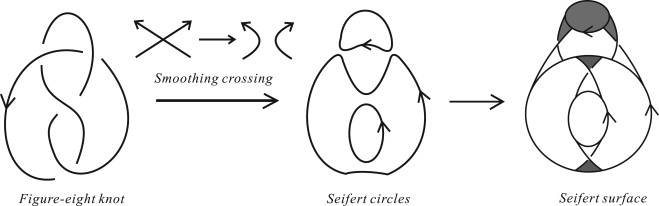
\includegraphics[width=0.75\textwidth]{../data/seifert-algorithm.jpg}
        \caption[Smthing]{Kolejne kroki algorytmu Seiferta}
    \end{figure}

    Dyski są dwustronne, więc ich górnej stronie przypisujemy znak $+$,
    jeśli tylko brzeg jest zorientowany dodatnio i~$-$ w~przeciwnym razie.
\index{algorytm!Seiferta|)}%
\end{proof}

Powierzchnia Seiferta dziedziczy orientację po węźle.
Nawet niewinne odwrócenie jednego z ogniw splotu potrafi istotnie zmienić jego powierzchnię, dlatego potrzebna jest ostrożność!

\index{powierzchnia!Seiferta|)}%

% Węzeł jest rozwłókniony dokładnie wtedy, gdy stanowi grzbiet pewnego 'open book decomposition' $S^3$.




\subsection{Węzły rozwłóknione}
\index{węzeł!włóknisty|see {węzeł rozwłókniony}}%
\index{węzeł!rozwłókniony|(}%
Wspomnijmy jeszcze krótko o~specjalnym rodzaju węzłów i splotów (patrz \cite[s. 49-50]{kawauchi96}).

% DICTIONARY;fibered;rozwłókniony, włóknisty;-
\begin{definition}
    Niech $L \subseteq S^3$ będzie splotem.
    Jeśli istnieje rodzina $F_t$ powierzchni Seiferta dla splotu $K$ sparametryzowana przez $t \in S^1$ taka, że $F_t \cap F_s = K$ dla $t \neq s$, to splot $K$ nazywamy rozwłóknionym albo włóknistym.
\end{definition}

\index{splot!Neuwirtha}%
Dawniej nazywano je splotami Neuwirtha, gdyż ten pokazał w~swojej pracy dyplomowej z~1959 roku, że można je scharakteryzować jako sploty, których komutant grupy podstawowej jest skończenie generowany, lub równoważnie, wolny.

\begin{example}
    Niewęzeł, trójlistnik $3_1$, ósemka $4_1$, $5_{1}$, $6_{2}$, $6_{3}$, $7_{1}$, $7_{6}$, $7_{7}$, $8_{2}$, $8_{5}$, $8_{7}$, $8_{9}$, $8_{10}$, $8_{12}$, $8_{16}$..$8_{21}$, splot Hopfa oraz wszystkie węzły torusowe są rozwłóknione.
\end{example}

(Jeśli węzeł pierwszy o co najwyżej ośmiu skrzyżowaniach nie został wymieniony w tym przykładzie, to nie jest rozwłókniony).
Rozkład liczby węzłów rozwłóknionych wśród węzłów pierwszych wygląda następująco:
\begin{itemize}
\item 9 skrzyżowań -- 23 węzły,
\item 10 skrzyżowań -- 74 węzły,
\item 11 skrzyżowań -- 256 węzłów,
\item 12 skrzyżowań -- 873 węzły.
\end{itemize}
% ZWERYFIKOWANO: funkcja count_fibered

Lwia część analizy węzłów o 12 skrzyżowaniach została wykonana przez Stojmenowa i~Hirasawę, jak podaje baza danych KnotInfo \cite{knotinfo22}.
% źródło: https://knotinfo.math.indiana.edu/descriptions/fibered.html
\index[persons]{Hirasawa, Mikami}%
\index[persons]{Stojmenow, Aleksander}%

\begin{proposition}
\index{wielomian!Alexandera}%
    Pierwszy i~ostatni współczynnik wielomianu Alexandera węzła rozwłóknionego to $\pm 1$.
\end{proposition}

% Kryterium to jest wystarczające dla węzłów pierwszych o co najwyżej 10 skrzyżowaniach oraz alternujących, ale znany jest przykład niewłóknistego węzła o 21 skrzyżowaniach, którego wielomian Alexandera ma postać $t^4 - t^3 + t^2 - t +1$.
% TODO: ustalić, czemu tak dużo skrzyżowań (z której książki ten fakt?). Sam wynik wydaje się być folklorem, tzn. nie wiadomo kto pierwszy to pokazał.

Kryterium to jest wystarczające dla węzłów pierwszych o co najwyżej 10 skrzyżowaniach, ale $11n_{34}$, $11n_{42}$, $11n_{73}$ oraz osiemnaście węzłów pierwszych o 12 skrzyżowaniach nie są rozwłóknione mimo tego, jak wygląda ich wielomian Alexandera.
% ZWERYFIKOWANO: funkcja alexander_fibered

\begin{example}
\index{węzeł!skręcony}%
    Niech $K$ będzie węzłem skręconym z $n$ półskrętami.
\index{wielomian!Alexandera}%
    Wtedy jego wielomianem Alexandera jest
    \begin{equation}
        \alexander_n(t) = n \cdot \left(t + \frac 1 t \right) - (2n+1),
    \end{equation}
    więc węzeł $K$ nie jest rozwłókniony, chyba że $n = 1$.
\end{example}

\begin{corollary}
% TODO: węzeł dokerski do indeksu?
    $2$-skręcony węzeł $6_1$ (węzeł dokerski) nie jest rozwłókniony.
\end{corollary}

Rolfsen \cite[s. 326]{rolfsen76} podaje jako ćwiczenie w swojej książce:

\begin{proposition}
\index{suma spójna}%
    Rodzina węzłów rozwłóknionych jest zamknięta na branie sum spójnych.
\end{proposition}

Dzięki książce Kawauchiego \cite[s. 84]{kawauchi96} wiem jeszcze, że Stallings ma swoje twierdzenie o~rozwłóknienieach dla zwartych 3-rozmaitości ze specjalnym przypadkiem:

\begin{proposition}
    Niech $y$ będzie jedynym epimorfizmem grupy splotu $L$ na nieskończoną grupę cykliczną $\langle t \rangle$, który posyła każdy południk na $t$. % each meridian
    Wtedy splot $L$ jest rozwłókniony wtedy i tylko wtedy, gdy jądro $\ker y$ jest skończenie generowalne.
\end{proposition}

\index{węzeł!rozwłókniony|)}%

% koniec podsekcji Węzły rozwłóknione




\subsection{Genus}
\index{genus|(}%
%label{sec:genus}%
Zanim przejdziemy do zdefiniowania macierzy Seiferta, potrzebować będziemy krótkiego skoku w bok -- zrozumieć bardzo geometryczny niezmiennik węzłów, genus.

Zaczniemy od starego twierdzenia, które klasyfikuje powierzchnie domknięte.

\begin{proposition}
    Każda powierzchnia domknięta jest członkiem jednej z dwóch nieskończonych rodzin:
    \begin{enumerate}[leftmargin=*]
        \itemsep0em
        \item sumą spójną $g \ge 0$ torusów,
        \item sumą spójną $k \ge 1$ rzeczywistych płaszczyzn rzutowych.
    \end{enumerate}
\end{proposition}

Elementy pierwszej rodziny są orientowalne.
Sferę traktujemy dla wygody jako sumę spójną $g = 0$ torusów.
Wtedy sumę spójną $g$ torusów możemy wyobrazić sobie jako sferę, do której doklejono $g$ uchwytów.

\begin{definition}[genus powierzchni]
    Ilość torusów nazywamy genusem powierzchni i oznaczamy literą $\genus$.
\end{definition}

Podobna charakteryzacja istnieje dla powierzchni z~brzegiem.
Każdy taki obiekt jest homeomorficzny z~sumą spójną $g$ torusów, w~których wydrążono pewną liczbę otworów: tyle, ile składowych spójności ma brzeg powierzchni.
W~przypadku powierzchni Seiferta mamy do czynienia z jednym otworem.

Dla wygody przypomnijmy jeszcze definicję klasycznego niezmiennika powierzchni:

\begin{definition}[charakterystyka Eulera]
\index{charakterystyka Eulera}%
    Niech $M$ będzie domkniętą powierzchnią orientowalną.
    Po striangulowaniu, składa się z $k_0$ wierzchołków, $k_1$ krawędzi oraz $k_2$ ścian.
    Wielkość
    \begin{equation}
        \chi = k_0 - k_1 + k_2
    \end{equation}
    jest niezmiennikiem powierzchni, zwanym charakterystyką Eulera.
\end{definition}

Definicja ta nie jest wygodna podczas ręcznych obliczeń.
Mamy za to:

\begin{proposition}
    Charakterystykę Eulera powierzchni jednoznacznie wyznaczają cztery reguły:
    \begin{itemize}
        \item jeśli $M$ jest dyskiem, to $\chi(M) = 1$,
        \item jeśli $M_1, M_2$ są powierzchniami, to $\chi(M_1 \sqcup M_2) = \chi(M_1) + \chi(M_2)$,
        \item jeśli powierzchnia $M_2$ powstaje z $M_1$ przez dołączenie paska, to $\chi(M_2) = \chi(M_1) - 1$,
        \item jeśli powierzchnia $M_2$ powstaje z $M_1$ przez dołączenie dysku do całej składowej spójności brzegu, to $\chi(M_2) = \chi(M_1) + 1$.
    \end{itemize}
\end{proposition}

Genus oraz charakterystyka Eulera są ze sobą związane:

\begin{proposition}
    Niech $M$ będzie powierzchnią o genusie $\genus$ i $\mu$ składowych spójności brzegu.
    Wtedy
    \begin{equation}
        \chi = 2 - \mu - 2\genus.
    \end{equation}
\end{proposition}

Nas interesują głównie powierzchnie Seiferta węzłów:
\index{powierzchnia Seiferta}%

\begin{proposition}
\label{prp:seifert_euler_characteristics}%
    Niech $K$ będzie węzłem z~diagramem $D$.
    Wtedy $\chi(M_D) = d - b$, gdzie $b$ jest liczbą skrzyżowań $D$, zaś $d$ jest liczbą okręgów Seiferta.
\end{proposition}

Można przeczytać o tym w \cite[s. 82]{murasugi96}.

\begin{proof}
    W~dowodzie faktu \ref{prp:seifert_exists} widzieliśmy, że liczba skrzyżowań $b$ jest jednocześnie liczbą pasków doklejonych do dysków.
    Bezpośredni rachunek pokazuje, że wtedy $k_0 = 4b$, $k_1 = 6b$ oraz $k_2 = b+d$.
    Wynika stąd, że $\chi = 4b - 6b + b + d = d - b$.
\end{proof}

Reszta tej podsekcji nie jest wymagana do zrozumienia macierzy Seiferta, przyjrzymy się genusowi jako obiektowi ciekawemu samemu w sobie.

\begin{definition}[3-genus]
    Niech $K$ będzie węzłem.
    Wśród wszystkich powierzchni Seiferta węzła $K$ istnieje co najmniej jedna o minimalnym genusie, jej genus nazywamy 3-genusem węzła $K$ i oznaczamy także przez $\genus$.
\end{definition}

Jeżeli nie powoduje to nieporozumień, zamiast 3-genus można pisać po prostu genus.

\begin{proposition}
\label{prp:genus_detects_unknot}%
    Genus wykrywa niewęzły: $K$ jest niewęzłem wtedy i tylko wtedy, gdy $g(K) = 0$.
\end{proposition}

\begin{proof}
    Niech $K$ będzie węzłem o genusie $0$.
    Z~charakteryzacji powierzchni wynika, że jego powierzchnia Seiferta to suma spójna $0$ torusów, to znaczy kula z tyloma otworami, ile $K$ ma ogniw.
    Innymi słowy, powierzchnią Seiferta węzła $K$ jest dysk, którego brzeg stanowi niewęzeł.
    To pokazuje, że implikacja w lewo jest prawdziwa.

    Implikacja w prawo jest oczywista.
\end{proof}

\subsubsection{Ograniczanie genusu z dołu}
Znalezienie 3-genusu dowolnego węzła sprawia te same trudności, co wyznaczenie jego liczby gordyjskiej.
Dowolna powierzchnia Seiferta zadaje ograniczenie z góry.
Z dołu 3-genus można szacować przy użyciu wielomianu Alexandera:
\index{wielomian!Alexandera}%

\begin{proposition}
\label{prp:alexander_genus}%
    Niech $K$ będzie węzłem.
    Wtedy $\operatorname{span} \alexander_K(t) \le 2\genus(K)$.
\end{proposition}

Fakt ten znalazłem w podręczniku Murasugiego \cite[s. 131]{murasugi96}.

\begin{proof}
    Załóżmy, że $F$ jest powierzchnią Seiferta węzła $K$ o genusie $g$.
    Wtedy macierz Seiferta powstała z $F$ jest stopnia $2g$, więc żaden ze składników jej wyznacznika nie może mieć stopnia (jako wielomian) większego niż $2g$.
\end{proof}

To dolne ograniczenie jest realizowane przez pewną powierzchnię Seiferta dla każdego pierwszego węzła o~co najwyżej 11 skrzyżowaniach poza siedmioma wyjątkami: 11n42, 11n67, 11n97 ($g = 2$), 11n34, 11n45, 11n73 oraz 11n152 ($g = 3$).
% warto byłoby dodać jakiś kod pozwalający sprawdzić, czemu akurat te węzły

\begin{proposition}
    Niech $K$ będzie węzłem, zaś $M$ jego macierzą Seiferta.
    Równość $\operatorname{span} \alexander_K(t) = 2\genus(K)$ zachodzi wtedy i tylko wtedy, gdy wyznacznik $\det M \neq 0$ jest niezerowy.
\end{proposition}

Floer zdefiniował w~\cite{floer90} przestrzeń wektorową nazywaną teraz homologią Floera, jest ona wyposażona w~endomorfizm parzystego stopnia, który powstaje z 2-wymiarowej klasy homologii reprezentowanej przez powierzchnię Seiferta.
%~kanoniczną gradację modulo $2$ oraz
\index{homologia!Floera}
Ta homologia rozkłada się na sumę prostą przestrzeni własnych wyróżnionego endomorfizmu, ich charakterystyki Eulera są współczynnikami wielomianu Alexandera.
Pozwala to na dokładniejsze szacowanie genusu węzła, patrz prace Ozsvátha, Szabó \cite{szabo03} i Ghigginiego \cite{ghiggini08}.
\index[persons]{Ghiggini, ?}%
\index[persons]{Ozsváth, Peter}%
\index[persons]{Szabó, Zoltán}%

\subsubsection{Ograniczanie genusu z góry}
Z góry genus ograniczony jest przez kilka klasycznych niezmienników numerycznych.
Zanim to pokażemy, przytoczymy techniczny lemat udowodniony przez Yamadę (\cite{yamada87}):
\index[persons]{Yamada, Shuji}%
% Morton MathSciNet: "The proof uses an ingenious direct algorithm to alter the projection without changing the number of Seifert circles"

\begin{proposition}
    \label{prp:seifert_circles_braid}
    Niech $L$ będzie splotem, zaś $\operatorname{s} L$ minimalną liczbą okręgów Seiferta, które dostajemy ze wszystkich możliwych diagramów splotu $L$.
    Wtedy $\operatorname{s} L = \braid L$ jest równe indeksowi warkoczowemu.
\index{indeks warkoczowy}%
\end{proposition}

Powyższe stwierdzenie występuje bez dowodu (bez?) w \cite[s. 17]{kawauchi96}.

\begin{proposition}
    Niech $L$ będzie splotem.
    Wtedy $\crossing L - \braid L - \operatorname{\mu} L + 2 \ge 2 \genus L$.
\end{proposition}

\begin{proof}
    Ustalmy minimalny diagram $D$ dla splotu $L$ i zastosujmy do niego algorytm Seiferta.
    Dostaniemy tak $s$ okręgów Seiferta oraz powierzchnię o genusie $g$.
    Fakt \ref{prp:seifert_euler_characteristics} mówiący, że $\chi = s - c$, można przekształcić do
    \begin{equation}
        g = \frac{c + 2 - s - \mu(K)}{2}.
    \end{equation}
    Z~minimalności diagramu wynika, że $c = \crossing L$.
    Fakt \ref{prp:seifert_circles_braid} mówi, że $s \ge \braid L$.
    Nierówność $g \ge \genus L$ wynika z~definicji genusu.
    Z powyższych rozważań wynika, że
    \begin{equation}
        \crossing L + 2 \ge 2 \genus L + \braid L + \operatorname{\mu} L,
    \end{equation}
    a to jest równoważnie nierówności, której prawdziwości dowodzimy.
\end{proof}

\begin{corollary}
    \label{cor:crossing_genus}
    Niech $K$ będzie węzłem.
    Wtedy $\crossing K \ge 2 \genus K$.
\index{indeks skrzyżowaniowy}
\end{corollary}

\subsubsection{Genus a rozkład na sumę węzłów pierwszych}

\begin{proposition}
    \label{prp:genus_of_sum}
    Jeśli $J, K$ są węzłami, to $g (J \shrap K) = g(J) + g(K)$.
\end{proposition}

Poniższy dowód pochodzi od Schuberta (\cite{schubert49}), został tylko zapisany we współczesnym języku.
\index[persons]{Schubert, Horst}%
Przebiega w dwóch etapach: najpierw pokazuje się, że genus sumy nie jest większy od sumy genusów składników, a następnie, że nie jest od niej mniejszy.

\begin{proof}
    Pokażemy najpierw, że $g(J \# K) \le g(J) + g(K)$.
    Wybierzmy powierzchnie Seiferta $M_J$ oraz $M_K$ dla $J$ oraz $K$ o~minimalnym genusie.
    Suma $J \shrap K$ powstaje z~$J$ oraz $K$, podobnie jest z~powierzchniami Seiferta:
\begin{comment}
    \begin{figure}[H]
        \centering
        \begin{minipage}[b]{.48\linewidth}
        \[
            \LargeGenusProofA \longrightarrow \LargeGenusProofB
        \]
        \subcaption{suma węzłów}
        %
        \end{minipage}
        \begin{minipage}[b]{.48\linewidth}
        \[
            \LargeGenusProofC \longrightarrow \LargeGenusProofD
        \]
        \subcaption{suma powierzchni}
        \end{minipage}
    \end{figure}
\end{comment}

    Skoro $M_{J\#K}$ powstaje z~$M_J \sqcup M_K$ przez dołączenie paska do brzegu, mamy
    \begin{equation}
        \chi(M_{J\#K}) = \chi(M_J \sqcup M_K) - 1 = \chi(M_J) + \chi(M_K)-1,
    \end{equation}
    a~przez to
    \begin{equation}
        g(M_{J\#K}) = \frac{1-\chi(M_{J\#K})}{2} =
        \frac{1-\chi(M_{J})}{2} + \frac{1-\chi(M_{K})}{2}
        % = %g(M_J)+g(M_K)
        = g(J) + g(K).
    \end{equation}
    To kończy dowód pierwszej nierówności.
    Pokażemy jeszcze, że $g(J \# K) \ge g(J)+g(K)$.
    Zaczynamy od powierzchni Seiferta $M_{J\#K}$ dla $J\#K$ o~minimalnym genusie $g(M_{J\#K})$ równym $g(J\#K)$.
    Poprzez wykonanie chirurgii na powierzchni, możemy przyjąć specjalną postać jak w~poprzednim dowodzie:
\begin{comment}
    \[
        \LargeGenusProofD
    \]
\end{comment}

    Usunięcie paska daje powierzchnie Seiferta dla $M_J$ oraz $M_K$ takie, że
    \begin{equation}
        g(M_J)+g(M_K)=g(M_{J\#K})=g(J\#K).
    \end{equation}
    Oznacza to, że $g(J) + g(K) \le g(M_J) + g(M_K) = g(J\#K)$ i~mamy równość.
\end{proof}

Jesteśmy wreszcie w~stanie podać prawdziwy dowód faktu \ref{first_time_sum_is_trivial}.

\begin{corollary}
    \label{cor:connected_sum_no_inverses}
    Jeśli suma spójna dwóch węzłów jest niewęzłem, to oba składniki także nim są.
\end{corollary}

Powrócimy teraz do węzłów pierwszych.
\index{węzeł!pierwszy}%

\begin{proposition}
    Niech $K$ będzie węzłem.
    Jeśli $g(K) = 1$, to $K$ jest węzłem pierwszym.
\end{proposition}

\begin{proof}
    Załóżmy nie wprost, że węzeł $K = K_1 \# K_2$ jest sumą dwóch nietrywialnych węzłów.
    Z~faktu \ref{prp:genus_of_sum} wynika wtedy, że $g(K) = g(K_1) + g(K_2)$.
    Zatem jeden z węzłów $K_1, K_2$ ma genus zero i jest trywialny, wbrew naszemu założeniu.
\end{proof}

Implikacja odwrotna jest fałszywa: pięciolistnik jest pierwszy, ale jego genus wynosi $2$.

\begin{proposition}
    Każdy węzeł można zapisać jako suma spójna pewnej liczby węzłów pierwszych.
    Niewęzeł jest sumą pustej rodziny węzłów.
\end{proposition}

\begin{proof}
    Dowodzimy przez indukcję względem genusu $g(K)$.
    Przypadek bazowy $g(K) = 0$ jest oczywisty, gdyż wtedy $K$ to niewęzeł.
    Załóżmy więc, że fakt zachodzi dla węzłów $J$ genusu co najwyżej $n$.
    Niech $K$ będzie genusu $n + 1$.

    Jeśli $K$ jest pierwszy, nie ma czego dowodzić.
    W przeciwnym razie jest równoważny z~$J_1 \shrap J_2$, gdzie $J_1$ i~$J_2$ są nietrywialne.
    Mamy $g(J_1) + g(J_2) = g(K)$ oraz $g(J_1),g(J_2) \ge 1$.
    Zatem $g(J_1), g(J_2) \le n$.
    Na mocy hipotezy indukcyjnej, $J_1$ oraz $J_2$ są równoważne sumom
    \[
        J_1 \cong K_1\#\cdots\# K_s,\qquad
        J_2 \cong K_{s+1}\#\cdots\# K_r,
    \]
    gdzie $K_i$ są pierwsze.
    Zatem $K$ jest równoważny z~$K_1\#\cdots\# K_r$, co kończy dowód.
\end{proof}

Nasz aparat matematyczny jest niedostatecznie rozwinięty, by móc udowodnić jedyność rozkładu.

\begin{theorem}[Schubert, 1949]
    Każdy nietrywialny węzeł rozkłada się na węzły pierwsze.
    Rozkład jest, z dokładnością do kolejności składników, jednoznaczny.
\index{węzeł!pierwszy}%
\end{theorem}

Schubert podał geometryczny dowód oparty o powierzchnie Seiferta; wyraził go w języku PL-rozmaitości (\cite{schubert49}), ale niedużym wysiłkiem można dokonać adaptacji do gładkiego świata.
\index[persons]{Schubert, Horst}%
Praca Schuberta korzysta z twierdzenia Alexandera, że 2-sfera w przestrzeni $\R^3$ ogranicza dysk, i jego odpowiednika dla torusów w $S^3$.

Hashizume \cite{hashizume58} rozszeszył wyniki Schuberta do splotów.
\index[persons]{Hashizume, ?}%
% trzeba wspomnieć, że to wymaga adaptacji definicji sumy spójnej, bo wcześniej dopuszczaliśmy tylko węzły jako składniki. Remedium = Kawauchi.

\begin{proposition}
    \label{prp:infinitely_many_prime_knots}
    Istnieje nieskończenie wiele węzłów pierwszych.
\end{proposition}

\begin{proof}
    Pokażemy, że wszystkie węzły $(2n+2)_1$ są pierwsze, gdzie $n \ge 1$.
    Istotnie, algorytm Seiferta zastosowany do diagramu tego węzła wyprodukuje $2n+1$ okręgów.
\begin{comment}
    \[
        \begin{tikzpicture}[baseline=-0.65ex,scale=0.06]
        \begin{knot}[clip width=7, flip crossing/.list={1,4,5},end tolerance=1pt]
            \node at (0,10) {$\cdots$};
            \strand[semithick] (-30, -5) -- (-5, -5);
            \strand[semithick]  (5, -5) -- (30, -5);
            \strand[semithick,latex-]  (-30,-15) -- (-5,-15);
            \strand[semithick]  (5,-15) -- (30,-15);

            \strand[semithick] (-5, -15) [in=down, out=right] to (5, -10) [in=right, out=up] to (-5, -5);
            \strand[semithick] (5, -15) [in=down, out=left] to (-5, -10) [in=left, out=up] to (5, -5);

            % zewnętrzne obręcze -- lewa strona
            \strand[semithick] (-30, 15) to [out=left, in=up]   (-45, 0);
            \strand[semithick] (-30,-15) to [out=left, in=down] (-45, 0);
            \strand[semithick] (-30,  5) to [out=left, in=up]   (-35, 0);
            \strand[semithick] (-30, -5) to [out=left, in=down] (-35, 0);

            % zewnętrzne obręcze -- prawastrona
            \strand[semithick] (30, 15) to [out=right, in=up]   (45,0);
            \strand[semithick] (30,-15) to [out=right, in=down] (45,0);
            \strand[semithick] (30,  5) to [out=right, in=up]   (35,0);
            \strand[semithick] (30, -5) to [out=right, in=down] (35,0);

            % jak w~drugim ruchu Reidemeistera - górny warkocz, lewy
            \strand[semithick] (-30, 15) [in=left, out=right] to (-20,  5);
            \strand[semithick] (-30,  5) [in=left, out=right] to (-20, 15);
            \strand[semithick] (-10, 15) [in=right, out=left] to (-20,  5);
            \strand[semithick] (-10,  5) [in=right, out=left] to (-20, 15);

            % jak w~drugim ruchu Reidemeistera - górny warkocz, prawy
            \strand[semithick] (30, 15) [in=right, out=left] to (20,  5);
            \strand[semithick] (10, 15) [in=left, out=right] to (20,  5);
            \strand[semithick] (30,  5) [in=right, out=left] to (20, 15);
            \strand[semithick] (10,  5) [in=left, out=right] to (20, 15);
        \end{knot}
        \end{tikzpicture}
        \longrightarrow
        \begin{tikzpicture}[baseline=-0.65ex,scale=0.055]
            \node at (0,10) {$\cdots$};
            \draw[semithick] (-30,  -5) -- (30, -5);
            \draw[semithick] (-30, -15) -- (30,-15);

            \draw[semithick] (0,-10) circle (3);

                % zewnętrzne obręcze -- lewa strona
            \draw[semithick] (-30, 15) to [out=left, in=up]   (-45, 0);
            \draw[semithick] (-30,-15) to [out=left, in=down] (-45, 0);
            \draw[semithick] (-30,  5) to [out=left, in=up]   (-35, 0);
            \draw[semithick] (-30, -5) to [out=left, in=down] (-35, 0);

                % zewnętrzne obręcze -- prawastrona
            \draw[semithick] (30, 15) to [out=right, in=up]   (45,0);
            \draw[semithick] (30,-15) to [out=right, in=down] (45,0);
            \draw[semithick] (30,  5) to [out=right, in=up]   (35,0);
            \draw[semithick] (30, -5) to [out=right, in=down] (35,0);

            \draw[semithick] (-30, 15) to [out=right, in=up] (-20,10);
            \draw[semithick] (-30,  5) to [out=right, in=down] (-20,10);

            \draw[semithick] (30, 15) to [out=left, in=up] (20,10);
            \draw[semithick] (30,  5) to [out=left, in=down] (20,10);

            \draw[semithick] (-10, 10) circle (5);
            \draw[semithick] (10,  10) circle (5);
        \end{tikzpicture}
    \]
\end{comment}
    Wynika stąd, że genus wynosi $\frac 12 (1 - (1+2n) + (2+2n)) = 1$, ponieważ wyznacznik ma wartość $4n+1$,
    węzły $(2n+2)_1$ nie są trywialne i~są parami różne.
\end{proof}

\subsubsection{Genus kanoniczny, genus wolny}
% DICTIONARY;free;wolny;genus
% DICTIONARY;canonical;kanoniczny;genus
% DICTIONARY;genus;genus;-
Czy w definicji genusu można ograniczyć się do tych powierzchni Seiferta, które pochodzą od algorytmu Seiferta?
Niestety, poza pewnymi wyjątkami, nie.
Zanim przekonamy się, dlaczego tak jest, zdefiniujmy jeszcze dwa niezmienniki.

\begin{definition}[genus kanoniczny]
\index{genus!kanoniczny}%
    Niech $K$ będzie węzłem.
    Najmniejszy z genusów powierzchni Seiferta węzła $K$, które pochodzą z~algorytmu Seiferta, nazywamy genusem klasycznym i~oznaczamy symbolem $\operatorname{g_c} K$ lub krótko $g_c$.
\end{definition}

Stojmenow \cite{stoimenow08} opisał diagramy węzłów o~kanonicznym genusie równym 2.
\index[persons]{Stojmenow, Aleksander}%
Część z~jego wyników przenosi się na genus 3.
Jak sam pisze, sklasyfikowane wcześniej węzły o~genusie (kanonicznym) 1 okazały się być zbyt wąską klasą.

Pod koniec lat pięćdziesiątych Crowell i~Murasugi niezależnie zauważyli, że algorytm Seiferta zastosowany do alternującego diagramu zawsze daje powierzchnię o~minimalnej powierzchni.
\index[persons]{Crowell, ?}%
\index[persons]{Murasugi, Kunio}%
Ich kombinatoryczne uzasadnienie było dość zawiłe, elementarny dowód podał Gabai w \cite{gabai86}.
\index[persons]{Gabai, David}%

Dubel trójlistnika ma genus równy $1$, ale algorytm Seiferta zastosowany wobec węzła produkuje powierzchnie o genusie co najmniej $3$, jak przewiduje ograniczenie znalezione przez Mortona w \cite[twierdzenie 2]{morton86}:

\begin{proposition}
    Niech $P(v, z)$ będzie wersją wielomianu HOMFLY spełniającą zależność
    \begin{equation}
        \frac 1v P_+ - vP_- = zP_0.
    \end{equation}
    Wtedy $M = \max \deg_z P(v, z) \le 2g_c$.
\end{proposition}

Nierówność Mortona jest równością dla wielu klas węzłów, w tym
\index{nierówność Mortona}%
alternujących (Crowell, Murasugi),
\index[persons]{Crowell, ?}%
\index[persons]{Murasugi, Kunio}%
\index{węzeł!alternujący}%
jednorodnych\footnote{Uogólnienie węzłów alternujących.} (Cromwell w \cite{cromwell89}),
\index{węzeł!jednorodny}%
\index[persons]{Cromwell, Peter}%
whiteheadowskich dubli węzłów dwumostowych (Nakamura w \cite{nakamura06}, Tripp w \cite{tripp02}) albo
\index{dubel Whiteheada}%
\index{węzeł!dwumostowy}%
\index[persons]{Nakamura, Takuji}%
\index[persons]{Tripp, ?}%
precli (Brittenham, Jensen \cite{brittenham06}).
\index[persons]{Brittenham, ?}%
\index[persons]{Jensen, ?}%
\index{precel}%
Stojmenow pokazał, że staje się równością dla węzłów o co najwyżej 12 skrzyżowaniach i znalazł przykład węzła, dla którego jest ostra.
\index[persons]{Stoimenow, Alexander}%

\begin{definition}[genus wolny]
\index{ciało z rączkami}%
\index{genus!wolny}%
    Niech $K$ będzie węzłem.
    Minimalny genus spośród powierzchni Seiferta węzła $K$, których dopełnienie w 3-sferze jest ciałem z rączkami, nazywamy genusem wolnym i~oznaczamy $g_f$.
\end{definition}

Dopełnienie powierzchni Seiferta jest zawsze ciałem z rączkami, więc mamy oczywiste nierówności
\begin{equation}
    g \le g_f \le g_c.
\end{equation}
Jak duża może być różnica między kolejnymi genusami?
Już Kirby \cite[problem 1.20a]{kirby78} chciał znać oszacowania różnicy $g_f - g$.
Morton \cite{morton86} pokazał, że genus pewnych węzłów nie jest realizowany przez żaden diagram do którego stosuje się algorytm Seiferta, choćby $10_{165}$.
Moriah, matematyk izraelski, rozwiązał problem Kirby'ego dekadę później:

\begin{proposition}
    Niech $K$ będzie węzłem, $D_k(K)$ jego dublem Whiteheada z $k \neq 0$ skręceniami, zaś $B_n(K)$ to $n$-krotne nakrycie cykliczne sfery $S^3$ rozgałęzione nad węzłem $K$.
    Jeżeli ranga pierwszej grupy homologii $B_{|4k+1|}(K)$ wynosi $r$, to
    \begin{equation}
        g_f(D_k(K)) \ge \frac {2r-1} {|8k+2|}.
    \end{equation}
\end{proposition}

\begin{proof}
    Praca \cite{moriah87}.
    Dowód opiera się na chirurgii węzłów i splotów w sferze $S^3$.
\end{proof}

\begin{corollary}
    Niech $K$ bedzie sumą spójną $n$ trójlistników, połóżmy $k = -1$.
    Wtedy pierwsza grupa homologii ma rangę $r = 2n$ i~genus wolny jest nieograniczony
    \begin{equation}
        g_f(D_{-1}(3_1^n)) \ge \frac {4n-1} {6},
    \end{equation}
    podczas gdy zwykły genus to $g(D_{-1}(3_1^n)) = 1$.
\end{corollary}

Kawauchi \cite{kawauchi94} zbadał węzeł $K_m$, sumę spójną $m$ kopii skręconego whiteheadowskiego dubla trójlistnika, i policzył, że różnica $g_c(K_m) - g(K_m)$ wynosi $2m$.
Wreszcie Kobayashi oraz Kobayashi \cite{kobayashi96} wskazali nieskończoną rodzinę węzłów nieograniczonego genusu, dla której
\begin{equation}
    g_c(K) = \frac 32 g_f(K) = 2g(K).
\end{equation}
% znam ich ze Stojmenow - Knots of (canonical) genus two

\index{genus|)}

% Koniec podsekcji Genus




\subsection{Macierz Seiferta}
\index{macierz Seiferta|(}
Niech $K$ będzie węzłem z diagramem $D$ i powierzchnią Seiferta $S$.

% Murasugi, s. 79
\begin{definition}[graf Seiferta]
\index{graf Seiferta}%
    Ściągnijmy dyski z dowodu faktu \ref{prp:seifert_exists} do punktów jednocześnie kurcząc doklejone paski, otrzymamy graf zwany grafem Seiferta diagramu $D$.
\end{definition}

Murasugi \cite[s. 79]{murasugi96} proponuje jako ćwiczenie dowód faktu:

\begin{proposition}
    Graf Seiferta jest dwudzielny i planarny.
\end{proposition}

% Murasugi 82, 83
Skoro graf Seiferta jest planarny, to dzieli sferę $S^2$ na $f$ obszarów.
Można wyznaczyć ich liczbę: skoro $\chi(S^2) = d - b + f = 2$, to $f - 1 = 1 - d + b$, pomijamy obszar nieograniczony.
Brzeg każdego obszaru jest zamkniętą krzywą, z których tworzymy krzywe $x_1, \ldots, x_m$ na powierzchni Seiferta.
Generują one grupę podstawową $\pi_1(S)$.

Niech $S$ będzie powierzchnią Seiferta z wyróżnioną jedną stroną.
Jeśli krzywa $x_i$ biegnie po powierzchni $S$, przez $x_i^*$ oznaczać będziemy dodatnie wypchnięcie: krzywą równoległą do $x_i$, która biegnie tuż nad nią.
Potrzebowaliśmy wyróżnić jedną ze stron powierzchni $S$, by słowo ,,nad'' miało sens.

\begin{definition}[macierz Seiferta]
    Przy zachowaniu powyższych oznaczeń, macierz, której wyrazy określa wzór $M_{i,j} = \operatorname{lk}(x_i, x_j^*)$, nazywamy macierzą Seiferta.
\end{definition}

Konstrukcja macierzy Seiferta zależy od wyboru diagramu oraz orientacji krzywych $x_i$, dlatego nie jest niezmiennikiem węzłów.
Stanie się nim, kiedy uwzględnimy jeszcze wpływ ruchów Reidemeistera.

\begin{proposition}
    Kwadratowa macierz $V$ o całkowitych wyrazach jest macierzą Seiferta węzła wtedy i~tylko wtedy, gdy $\det(V - V^t) = 1$.
\end{proposition}

\begin{proof}
    Kawauchi \cite[s. 62]{kawauchi96} pisze, że wynika to z~klasyfikacji macierzy Seiferta splotów.
\end{proof}

\begin{definition}
    Operacja $\Lambda_1$ dla pewnej odwracalnej macierzy $P$ o całkowitych wyrazach (czyli $\det P = \pm 1$) to
    \begin{equation}
        \Lambda_1 \colon M \mapsto PMP^t.
    \end{equation}
    Natomiast operację $\Lambda_2$ definiuje wzór:
    \begin{equation}
        \Lambda_2 \colon M \mapsto \begin{bmatrix}
  &   &  & 0 & 0 \\
  & M &  & \vdots & \vdots \\
  &   &  & 0 & 0 \\
* & \dots & * & 0 & 0 \\
0 & \dots & 0 & 1 & 0
\end{bmatrix} \textrm{albo} \begin{bmatrix}
  &   &  & * & 0 \\
  & M &  & \vdots & \vdots \\
  &   &  & * & 0 \\
0 & \dots & 0 & 0 & 1 \\
0 & \dots & 0 & 0 & 0
\end{bmatrix},
    \end{equation}
    gdzie gwiazdka zastępuje ustaloną liczbę całkowitą.
\end{definition}

\begin{definition}
\index{S-równoważność}%
    Niech $M_1, M_2$ będą macierzami.
    Jeśli $M_2$ można otrzymać z $M_1$ przez skończony ciąg operacji $\Lambda_1, \Lambda_2$ oraz ich odwrotności, to macierze nazywamy $S$-równoważnymi.
\end{definition}

Badania powyższej relacji równoważności prowadzili w~latach sześćdziesiątych ubiegłego stulecia Trotter \cite{trotter62}, Murasugi \cite{murasugi65} oraz Levine \cite{levine70}.
\index{człowiek!Trotter, Hale}%
\index{człowiek!Murasugi, Kunio}%
\index{człowiek!Levine, Jerome}%
Litera $S$, jak nietrudno się domyślić, pochodzi od Seiferta.

\begin{proposition}
    Macierz Seiferta modulo $S$-równoważność jest niezmiennikiem splotów.
\end{proposition}

Dowód tego faktu jest elementarny, ale dość długi.
Razem z~ułatwiającymi zrozumienie diagramami można znaleźć go w podręczniku Murasugiego albo \cite[s. 64]{kawauchi96}, dlatego pomijamy go i skupimy się na tym, jakie niezmienniki można otrzymać z macierzy Seiferta.

Wyznacznik całej macierzy Seiferta nie jest niezmiennikiem.
Wykonując operację $\Lambda_2$ dostajemy macierz, której ostatnia kolumna albo ostatni wiersz są zerami, więc jej wyznacznik także jest zerem.
Jeśli jednak najpierw dokonamy jej symetryzacji, dostaniemy znany już niezmiennik.

\begin{proposition}
    Niech $M$ będzie macierzą Seiferta węzła $K$.
    Wtedy
    \begin{equation}
        \det K = |\det(M + M^t)|.
    \end{equation}
\end{proposition}

\index{wielomian!Alexandera}%
Przez wprowadzenie dodatkowej zmiennej $t \in \R$, ponownie uogólnimy wyznacznik do wielomianu Alexandera.

\begin{proposition}
    Niech $M$ będzie macierzą Seiferta stopnia $k$ węzła $K$.
    Wtedy
    \begin{equation}
        \alexander_K (t) = t^{-k/2}\det(M - tM^t).
    \end{equation}
\end{proposition}

Określimy jeszcze dwa, niewystępujący wcześniej niezmiennik (Arfa i sygnaturę).

\index{macierz Seiferta|)}




\subsection{Sygnatura}
\label{sub:signature}%
\index{sygnatura|(}%
Sygnatura jest kolejnym niezmiennikiem, do zdefiniowania których wystarczy znać macierz Seiferta.
Pochodzi prawdopodobnie z lat sześćdziesiątych (Trotter \cite{trotter62} dla węzłów, Murasugi \cite{murasugi65} dla splotów).
\index[persons]{Trotter, Hale}%
\index[persons]{Murasugi, Kunio}%
% z recenzji do 275415: Shinohara, Yaichi - On the signature of knots and links.
Ktoś powiedział nam kiedyś, że ujednolicenia różnych podejść do form kwadratowych związanych z węzłami dokonali Gordon, Litherland, Murasugi w~pracy \cite{litherland81}, ale potem trafiliśmy na artykuł Przytyckiego \cite{przytycki11} pełen historycznych ciekawostek oraz dwóch kolejnych odnośników: do wspomnianej przed chwilą pracy \cite{murasugi65}, ale też \cite{litherland78} samych Gordona, Litherlanda, którzy sięgają zenitu i wiążą dziełą Goeritza, Trottera, Murasugiego et alli.
Może po prostu najlepiej przeczytać wszystko?

% DICTIONARY;signature;sygnatura;-
\begin{definition}[sygnatura]
\label{def:signature}%
    Niech $M$ będzie macierzą Seiferta zorientowanego splotu $L$.
    Wielkość
    \begin{equation}
        \sigma_L := \operatorname{\sigma} (M + M^t),
    \end{equation}
    sygnaturę macierzy $M + M^t$, nazywamy sygnaturą splotu $L$.
\end{definition}

\begin{proposition}
\label{prp:signature_additive}%
    Sygnatura jest addytywna: $\sigma(K_1 \shrap \ldots \shrap K_n) = \sum_{k=1}^n \sigma(K_k)$.
\end{proposition}

Wiem o tym z \cite[s. 127]{murasugi96}.

\begin{proof}
    Bez straty ogólności ograniczmy się do przypadku $n = 2$ i~ustalmy powierzchnie Seiferta $F_1, F_2$ dla węzłów $K_1, K_2$ z~macierzami Seiferta $M_1, M_2$.
    Powierzchnia dla ich sumy spójnej $K_1 \shrap K_2$ powstaje przez sklejenie $F_1$ oraz $F_2$ paskiem.
    W języku macierzy oznacza to, że macierz Seiferta węzła $K_1 \shrap K_2$ ma postać $M = M_1 \oplus M_2$.
    Zatem:
    \begin{align}
        \sigma(K_1 \shrap K_2) & = \sigma(M + M^t) \\
                               & = \sigma(M_1 + M_1^t) + \sigma(M_2 + M_2^t) \\
                               & = \sigma(K_1) + \sigma(K_2),
    \end{align}
    co kończy dowód.
\end{proof}

\begin{corollary}
\index{liczba mostowa}%
\label{no_relation_signature_bridge}%
    Nie istnieje bezpośredni związek między sygnaturą i~liczbą mostową.
\end{corollary}

Patrz \cite[s. 145]{livingston93}.

\begin{proof}
    Węzeł torusowy $T_{2,n}$ jest dwumostowy, jego sygnatura wynosi $n - 1$.
    Suma spójna węzłów prostych (sumy przeciwnie zorientowanych trójlistników) ma zerową sygnaturę, ale na mocy faktu~\ref{prp:bridge_additive} jej liczba mostowa jest nieograniczona.
\end{proof}

\begin{proposition}
\index{lustro}%
\index{rewers}%
\label{prp:signature_mirror_reverse}%
    Niech $L$ będzie splotem.
    Wtedy $\sigma(mL) = -\sigma(L)$ oraz $\sigma(rL) = \sigma(L)$.
\end{proposition}

O tym także wiem z \cite[s. 127]{murasugi96}.

\begin{proof}
    Wynika to z podobnych faktów dla macierzy Seiferta.
    Równoważność $M_{mL} \simeq - M_L^t$ wynika z tego, że zamiana nad- i podskrzyżowań odwraca wzajemne położenie krzywych, których indeksu zaczepienia szukamy.

    Podobnie pokazuje się, że $M_{rL} \simeq M_L^t$.
\end{proof}

\begin{corollary}
\index{węzeł!achiralny}%
\label{cor:acheiral_signature}%
    Jeśli $K$ jest węzłem achiralnym, to $\sigma(K) = 0$.
\end{corollary}

Węzły achiralne mają zerową sygnaturę, zatem trójlistnik nie jest achiralny.
Z faktów~\ref{prp:signature_additive} oraz~\ref{prp:signature_mirror_reverse} wynika, że suma tak samo zorientowanych trójlistników nie jest achiralna ($\sigma = \pm 4$).
Jak można przekonać się ze standardowego diagramu węzła prostego, ten jest achiralny.
Pisaliśmy coś o tym na stronie \pageref{two_sums_of_two_trefoils}.

\begin{proposition}
\label{trivial_alexander_polynomial}%
\index{wielomian!Alexandera}%
    Niech $L$ będzie węzłem.
    Jeśli $\alexander_K(t) \equiv 1$, to $\sigma (K) = 0$.
\end{proposition}

Założenie $\alexander_K(t) \equiv 1$ jest spełnione przez cztery węzły pierwsze do 12 skrzyżowań, są to $11n_{34}, 11n_{42}, 12n_{313}$ oraz $12n_{430}$, patrz wzmianka po fakcie~\ref{alexander_no_detects_unknot}.
% ZWERYFIKOWANO: funkcja trivial_alexander

\begin{proof}
\index[persons]{Milnor, John}%
    Murasugi twierdzi, że zostało to udowodnione przez Milnora w \cite{milnor68}, nie jesteśmy jednak pewni, gdzie dokładnie, ale raczej poza sekcją piątą.
\end{proof}

Istnieje równoważna definicja, która nie wymaga czasochłonnego wyznaczania macierzy Seiferta.

\begin{proposition}
\index{relacja kłębiasta}%
    Sygnatura to niezmiennik topologiczny zadany kłębiastą relacją rekurencyjną:
    \begin{itemize}[leftmargin=*]
    \itemsep0em
        \item $\sigma (\SmallUnknot) = 0$,
        \item $\sigma (K_+) - \sigma (K_-) \in \{0, 2\}$,
        \item $4 \mid \sigma (K)$ wtedy i~tylko wtedy, gdy $\conway(2i) > 0$ (wielomian Conwaya).
    \end{itemize}
\end{proposition}

Symbole $K_+, K_-$ objaśnione są przy definicji~\ref{skein_symbols}.

\begin{proof}
    Wystarczy pokazać, że sygnatura węzła spełnia trzy powyższe aksjomaty, a~następnie zauważyć, że korzystając z~nich jesteśmy w~stanie wyznaczyć jednoznacznie sygnaturę dla dowolnego węzła.
    Wynika to z~faktu, że każdy węzeł można zmienić w~niewęzeł odwracając pewne skrzyżowania.
    Pomysł opisał dokładnie Giller \cite[trzecie spostrzeżenie]{giller82}, sam oparł się o~\cite[twierdzenie 5.6]{murasugi65}.
\index[persons]{Giller, Cole}%
\end{proof}

Sygnatura pozwala uzyskać proste oszacowanie liczby gordyjskiej od dołu:
\index{liczba gordyjska}%

\begin{proposition}
    Mamy $2 u(K) \ge |\sigma(K)|$.
\end{proposition}

Liczba gordyjska 83 z~801 węzłów pierwszych o mniej niż dwunastu skrzyżowaniach nie jest jeszcze znana.
Dla 272 spośród pozostałych mamy równość $2u = |\sigma|$.
% ZWERYFIKOWANO: funkcja unknotting_sigma 

\begin{proof}
    Ustalmy diagram $D$ dla węzła $K$.
    Odwrócenie dowolnego skrzyżowania polega na przejściu z~diagramu $D_+$ do $D_-$ lub z~$D_-$ do $D_+$.
    Zgodnie z relacją kłębiastą, sygnatura pozostaje taka sama lub zmienia wartość o $2$.
    Po wykonaniu $u$ odwróceń otrzymujemy diagram niewęzła o~sygnaturze zero, zatem sygnatura wyjściowego węzła nie mogła przekraczać $2u$.
    To kończy dowód.
\end{proof}

W~\cite{shinohara71} Shinohara pokazał, że dla każdej pary nieujemnych liczb całkowitych $m, n$ istnieje węzeł $K$ o wyznaczniku $4m+1$ ($8m+5$, $4m+3$) oraz sygnaturze bez znaku $8n$ ($8n+4$, $4n+2$).
\index[persons]{Shinohara, Yaichi}%
\index{wyznacznik}%
Ponadto, jeśli $m$ nie dzieli się przez $3$, istnieje węzeł o wyznaczniku $8m+1$ i sygnaturze bez znaku $8n+4$.
% skąd to? Ohtsuki?

Czas na raczej niezbyt użyteczną ciekawostkę.

\begin{conjecture}
    Czy istnieje węzeł o~sygnaturze $4$ i~wyznaczniku postaci $n = 4k + 1$?
\end{conjecture}

Stojmenow twierdzi, że jeśli tak jest, to wszystkie pierwsze dzielniki $n$ dają resztę $1$ z~dzielenia przez $24$ i~są większe od $2857$.
\index[persons]{Stojmenow, Aleksander}%
Patrz \cite[s. 540]{ohtsuki02}.

Czytając przeglądową pracę Conwaya \cite{conway19} dowiedzieliśmy się, że w~latach sześćdziesiątych sygnatura została uogólniona do funkcji $\sigma_L \colon S^1 \to \Z$.
\index[persons]{Conway, John}%
Większość podręczników, a także prace Levine'a \cite{levine69} oraz Tristrama \cite{tristram69}, wprowadza ją przy użyciu macierzy Seiferta, więc my postąpimy dokładnie tak samo.
\index[persons]{Levine, Jerome}%
\index[persons]{Tristram, Andrew}%

\begin{definition}[sygnatura Levine'a-Tristrama]
\index{sygnatura!Levine'a-Tristrama}%
    Niech $M$ będzie macierzą Seiferta zorientowanego splotu $L$.
    Funkcję $\sigma_L \colon S^1 \to \Z$ daną wzorem
    \begin{equation}
        \sigma_L(\omega) := \operatorname{\sigma} [(1-\omega) M + (1 - \overline{\omega})M^t]
    \end{equation}
    nazywamy sygnaturą Levine'a-Tristrama splotu $L$.
    Jest niezmiennikiem splotów.
\end{definition}

Funkcja $\sigma_L$ jest kawałkami stała.
Conway pisze w \cite{conway19}, że wynika to ze wzoru na wielomian Alexandera $\Delta_L(t) = \det(tM - M^t)$.
\index[persons]{Conway, John}%
\index{wielomian!Alexandera}%
Jedynymi punktami nieciągłości są zera wielomianu $(t-1)\Delta_L(t)$, to świeży wynik Gilmera, Livingstona z~\cite{gilmer16}.
\index[persons]{Gilmer, Patrick}%
\index[persons]{Livingston, Charles}%

Mówimy, że funkcja zdefiniowana na okręgu jest zbalansowana, jeżeli w każdym punkcie nieciągłości przyjmuje wartość równą średniej z~lewo- oraz prawostronnej granicy w tym punkcie.
Livingston podał pełną charakteryzację zbilansowanych sygnatur Levine'a-Tristrama dla węzłów, analogiczny problem dla splotów wydaje się być wciąż otwarty.

\begin{proposition}
\label{balanced_iff_four_conditions}%
    Funkcja zbalansowana $\sigma \colon S^1 \to \Z$ jest realizowana jako sygnatura pewnego węzła wtedy i tylko wtedy, gdy:
    \begin{enumerate}
        \item dla każdego $\omega \in S^1$ mamy $\sigma(\omega) = \sigma(\overline{\omega})$
        \item $\sigma(1) = 0$
        \item każda nieciągłość funkcji $\sigma$ jest miejscem zerowym wielomianu Alexandera węzła
        \item jeżeli argumenty $\omega_1, \omega_2$ są sprzężone w sensie Galois, to $\sigma(\omega_1) \equiv \sigma(\omega_2)$ modulo $2$.
    \end{enumerate}
\end{proposition}

\begin{proof}
    Livingston pisze w \cite{livingston18}, że dowód w prawą stronę jest dość dobrze znany, natomiast w lewo korzysta z~wyników Kondo \cite{kondo79} i Sakaiego \cite{sakai77}, że każdy wielomian Alexandera węzła jest realizowany przez węzeł 1-gordyjski oraz zachowania zbalansowanej sygnatury podczas odwracania skrzyżowania.
\end{proof}

(Nie każdy wielomian Kauffmana/HOMFLY jest realizowany przez węzły 1-gordyjskie, Kawauchi \cite[s. 151]{kawauchi96} wspomina na przykład, że $\unknotting K \ge \log_3 |Q(-1)|$.)

\begin{proposition}
\index{węzeł!satelitarny}%
    Niech $S$ będzie satelitą z towarzyszem $C$, wzorcem $P$ oraz indeksem zaczepenia $n$.
    Wtedy
    \begin{equation}
        \sigma_S(\omega) = \sigma_P(\omega) + \sigma_C(\omega^n).
    \end{equation}
\end{proposition}

\begin{proof}
    Szczególny przypadek $\omega = -1$ rozpatrywał wcześniej Shinohara w~\cite{shinohara71}.
\index[persons]{Shinohara, Yaichi}%
    Pełny dowód znajduje się w artykule \cite{litherland79} Litherlanda.
\index[persons]{Litherland, Richard}%
\end{proof}

Wreszcie:

\begin{proposition}
    Niech $L$ będzie splotem.
    Wtedy albo wielomian Alexandera $\Delta_L(t)$ jest tożsamościowo zerem, albo posiada co najmniej $|\sigma_L|$ zer, liczonych z krotnościami, na okręgu jednostkowym.
\end{proposition}

\begin{proof}
    Aneks w książce Liechtiego \cite{liechti16}, która nie wygląda na związaną z~teorią węzłów.
\end{proof}

\index{sygnatura|)}%

% Koniec podsekcji Sygnatura



% koniec sekcji Powierzchnie Seiferta


\section{Niezmiennik Arfa}
\index{niezmiennik!Arfa|(}

Cahit Arf wprowadził w 1941 roku pewien niezmiennik nieosobliwych form kwadratowych nad ciałem charakterystyki dwu.
Zrobił to między innymi po to, by sklasyfikować takie formy kwadratowe.
My poznamy wariant niezmiennika Arfy dla węzłów.

Niech $(v_{i,j})$ będzie macierzą Seiferta węzła $K$ o genusie $g$.
Wtedy jej wymiary wynoszą $2g \times 2g$ i macierz $V-V^t$ jest symplektyczna.

\begin{definition}
    Zachowując powyższe oznaczenia, niezmiennik Arfa to
    \begin{equation}
        \sum^g_{i=1}v_{2i-1,2i-1}v_{2i,2i} \pmod 2.
    \end{equation}
    % Przyjmuje on dwie wartości: 0, 1
\end{definition}

Niezmiennik Arfa dla węzłów można zdefiniować na kilka sposobów, z~których żaden nie jest istotnie lepszy od pozostałych.
Pierwszy był pomysł Robertello \cite{robertello65}:

\begin{proposition}[Robertello, 1965]
    Niech $K$ będzie węzłem, zaś
    \begin{equation}
        \alexander_K(t)=c_{0}+c_{1}t+\cdots +c_{n}t^{n}+\cdots +c_{0}t^{2n}
    \end{equation}
    jego wielomianem Alexandera.
    Wtedy niezmiennik Arfa to $c_{n-1}+c_{n-3}+\cdots +c_{r} \mod 2$, gdzie $r = 0$ dla nieparzystych $n$, $r = 1$ w~przeciwnym razie.
\end{proposition}

Nieco później Murasugi \cite{murasugi69} zauważył, że warunek można uprościć:

\begin{proposition}[Murasugi, 1969]
    \label{prp:arf_murasugi}
    Niech $K$ będzie węzłem.
    Wtedy $\operatorname{Arf} K = 0$ wtedy i~tylko wtedy, gdy $\alexander_K(-1) \equiv \pm 1 \mod 8$.
\end{proposition}

Kauffman zaproponował inne podejście z wykorzystaniem diagramów.
Dwa węzły nazwiemy równoważnymi przez przejścia, jeśli są związane skończenie wieloma ,,przejściami'' \cite[s. 143]{kauffman83}:
\begin{comment}
\[
    \begin{tikzpicture}[baseline=-0.65ex,scale=0.35]
    \begin{knot}[clip width=7]
        \strand[-latex, thick] (-2.5,-1.0) to (2.5,-1.0);
        \strand[-latex, thick] (2.5,1.0) to (-2.5,1.0);
        \strand[-latex, thick] (-1.0,-2.5) to (-1.0,2.5);
        \strand[-latex, thick] (1.0,2.5) to (1.0,-2.5);
    \end{knot}
    \end{tikzpicture}
    \cong
    \begin{tikzpicture}[baseline=-0.65ex,scale=0.35]
    \begin{knot}[clip width=7, flip crossing/.list={1,2,3,4}]
        \strand[-latex, thick] (-2.5,-1.0) to (2.5,-1.0);
        \strand[-latex, thick] (2.5,1.0) to (-2.5,1.0);
        \strand[-latex, thick] (-1.0,-2.5) to (-1.0,2.5);
        \strand[-latex, thick] (1.0,2.5) to (1.0,-2.5);
    \end{knot}
    \end{tikzpicture}
    \quad\mbox{albo}\quad
    \begin{tikzpicture}[baseline=-0.65ex,scale=0.35]
    \begin{knot}[clip width=7]
        \strand[-latex, thick] (-2.5,-1.0) to (2.5,-1.0);
        \strand[-latex, thick] (2.5,1.0) to (-2.5,1.0);
        \strand[latex-, thick] (-1.0,-2.5) to (-1.0,2.5);
        \strand[latex-, thick] (1.0,2.5) to (1.0,-2.5);
    \end{knot}
    \end{tikzpicture}
    \cong
    \begin{tikzpicture}[baseline=-0.65ex,scale=0.35]
    \begin{knot}[clip width=7, flip crossing/.list={1,2,3,4}]
        \strand[-latex, thick] (-2.5,-1.0) to (2.5,-1.0);
        \strand[-latex, thick] (2.5,1.0) to (-2.5,1.0);
        \strand[latex-, thick] (-1.0,-2.5) to (-1.0,2.5);
        \strand[latex-, thick] (1.0,2.5) to (1.0,-2.5);
    \end{knot}
    \end{tikzpicture}
\]
\end{comment}

\begin{definition}[Kauffman, 1983]
    Każdy węzeł $K$ jest równoważny przez przejścia albo z niewęzłem (wtedy mówimy, że $\operatorname{Arf} K = 0$), albo z trójlistnikiem (wtedy, że $\operatorname{Arf} K = 1$).
\end{definition}

Wreszcie Jones zauważył \cite{jones85}, że wielomian $\jones$ także pozwala na określenie niezmiennika Arfa, dzięki zespolonym algebrom Clifforda oraz pracy \cite{lannes85}.
Jest to jedyna definicja, którą łatwo rozszerzyć do splotów.

\begin{proposition}[Jones, 1985]
\label{prp:arf_jones}%
    $\operatorname{Arf}(K) = \jones_K(i)$.
\end{proposition}

\begin{corollary}
    Niezmiennik Arfa jest $\shrap$-addytywny (modulo 2).
\end{corollary}

\begin{proof}
    Wynika to z faktu \ref{prp:arf_jones} oraz \ref{prp:jones_multiplicative_2}, ale bezpośredni dowód też istnieje. % gdzie?
\end{proof}

O niezmienniku Arfa usłyszymy jeszcze poznając węzły plastrowe.

\index{niezmiennik!Arfa|)}

% Koniec sekcji Niezmiennik Arfa

\section{Homologie}

Ta sekcja wymaga znajomości przynajmniej homologii: kompleksów łańcuchowych, różniczek, grup homologii.
Można się tego nauczyć z~każdego podręcznika topologii algebraicznej.

\subsection{Homologie Chowanowa}
\index{homologia!Chowanowa|(}
Viro napisał w 2004 piękną pracę \cite{viro04}, by objaśnić homologię Chowanowa używając tak mało algebry, jak to tylko możliwe.
Jest przyjazna dla początkujących, więc na niej opiera się reszta tej podsekcji\footnote{Viro wymienia kilka innych artykułów, z których można czerpać wiedzę. \emph{,,A good place to start: \cite{barnatan02} followed by \cite{shumakovitch12}, \cite{khovanov00}. Another possible starting point: \cite{turner17}.''}}.
Będziemy pracować ze stanami Kauffmana i obramowanymi węzłami, ponieważ autor sugeruje, że to bardziej naturalne.
Oryginalna praca Chowanowa to \cite{khovanov00}.

Niech $L$ będzie splotem, zaś $D$ jego diagramem.
Chowanow skonstruował rodzinę grup $\mathcal H^{i, j}(D)$ takich, że
\begin{equation}
    K(L, q) = \sum_{i, j} q^j (-1)^i \dim_\Q (\mathcal H^{i, j}(D) \otimes \Q),
\end{equation}
gdzie $K$ jest wersją wielomianu Jonesa.
Grupy $\mathcal H^{i, j}$ są u~niego grupami homologii pewnych kompleksów łańcuchowych.
Ich konstrukcja była przeładowana algebraicznymi szczegółami, później Bar-Natan \cite{barnatan02}, Viro podali jej warianty z~myślą o~topologach.
% Viro - Remarks on definition of Khovanov homology, arXiv

Homologię Chowanowa nazywa się kategoryfikacją wielomianu Jonesa.
Zanim zagłębimy się w szczegóły, rozpatrzmy prostszy przykład tego procesu.
Niech $X$ będzie przestrzenią topologiczną, wtedy charakterystykę Eulera oraz grupy homologii łączy zależność
\begin{equation}
    \chi(X) = \sum_{n = 0}^{\dim X} (-1)^n \operatorname{rk} H_n(X),
\end{equation}
a przy tym grupy homologii dostarczają więcej informacji, co więcej można o nich myśleć jako funktorach.
Homologie są kategoryfikacją charakterystyki Eulera.

Kategoryfikacja wielomianu Jonesa polega na zastąpieniu jakoś jego współczynników przez ciąg grup abelowych.
Wzór o sumowaniu stanów przypomina ostatnią równość, brakuje tylko przedstawienia składników po prawej stronie jako alternująca suma rang grup.

Viro zauważa, że powszechna definicja wielomianu Jonesa sprawia problem dla pustego splotu (którego nigdy wcześniej nie rozpatrywaliśmy).
Mamy:
\begin{equation}
    \jones_\varnothing = \frac{1}{-t^{1/2} - t^{-1/2}},
\end{equation}
a to nie jest wielomian Laurenta jednej zmiennej.
\index{wielomian Jonesa!powiększony}%
Dlatego definiuje powiększony wielomian Jonesa:
\begin{equation}
    \widetilde{\jones_L}(t) = (-t^{1/2} - t^{-1/2}) \cdot \jones_L(t),
\end{equation}
i mówi, że będzie kategoryfikować powiększony wielomian Jonesa, a właściwie powiększoną klamrę Kauffmana.

Jak pisze dalej, pewne drobne trudności techniczne mogły skłonić Chowanowa do pozbycia się ułamkowych potęg przez zmianę zmiennej w~powiększonym wielomianie Jonesa: niech $q := -t^{1/2}$.
Dostaje się tak nowy wielomian, nazwijmy go $K$.
Spełnia trzy aksjomaty:
\begin{itemize}
\item (normalizacja) $K(\SmallUnknot) = q + 1/q$;
\item (stabilizacja) $K(L \sqcup \SmallUnknot) = (q + 1/q) K(L)$;
\item (relacja kłębiasta) \begin{equation}
    q^{-2}     K\left( \MediumPlusCrossingArrows \right) -
    q^{2}      K\left( \MediumMinusCrossingArrows \right) =
    (q^{-1}-q) K\left( \MediumJustSmoothing \right).
\end{equation}
\end{itemize}

Stąd widać już, jakie grupy dobrać dla niewęzła:
\begin{equation}
    H^{i,j} = \begin{cases}
        \Z & \textrm{ jeśli } i = 0, j = \pm 1 \\
        0  & \textrm{ w przeciwnym razie}.
    \end{cases}
\end{equation}
Wtedy spełniona jest równość
\begin{equation}
    K(L, q) = \sum_{i, j} (-1)^i q^j \operatorname{rk} H^{i, j} (L).
\end{equation}
Pozostało powtórzyć to dla dowolnego splotu.
Wzór o sumowaniu stanów przybiera postać:
\begin{equation}
    K(L, q) = \sum_s (-1)^{(\writhe D - |s|)/2} q^{(3\writhe D - |s|)/2} (q+1/q)^{|sD|}.
\end{equation}

Reprezentacja ta ma jedną wadę: każdy składnik z prawej strony przyczynia się do różnych jednomianów, zatem ma wpływ na różne grupy (których dopiero szukamy).
,,Surowe'' stany nie są prawdziwym odpowiednikiem sympleksów, jakie spotyka się podczas kategoryfikacji charakterystyki Eulera.
Najprostszym pomysłem, jak to naprawić, jest rozbicie ostatniej potęgi $q + 1/q$.
Zauważmy, że ma tyle czynników, ile wygładzenie diagramu ma składowych.
To motywuje definicję:

\begin{definition}[stan wzbogacony]
\index{stan!wzbogacony}%
    Stan diagramu $D$ razem z przypisaniem znaku $+$ lub $-$ do każdego okręgu $sD$ nazywamy stanem wzbogaconym.
\end{definition}

Dla ustalonego wzbogaconego stanu $S$ diagramu $D$ oznaczmy przez $\tau(S)$ sumę znaków przypisanych do okręgów\footnote{Oznaczenie wzięte z pracy Viro, żywimy nadzieję, że nikt nie weźmie $\tau$ za liczbę kolorowań z rodziału drugiego. Poza tym, Viro pisze $\sigma(s)$ zamiast naszego $|s|$ oraz $|s|$ zamiast naszego $|sD|$. Ostrożność wskazana.}.
Wtedy
\begin{equation}
    q^{(3 \writhe D - |s|)/2} (q + 1/q)^{|sD|} = \sum_{S/s} q^{(3 \writhe D - |s| + 2 \tau(S))/2},
\end{equation}
gdzie sumowanie odbywa się po wszystkich stanach $S$ wzbogacających stan $s$.
Niech
\begin{equation}
    j(S) := \frac 12 (3 \writhe D - |s| + 2 \tau(S)).
\end{equation}
Dobrnęliśmy do
\begin{equation}
    K(L, q) = \sum_S (-1)^{(\writhe D - |s|)/2} q^{j(S)},
\end{equation}
tym razem sumujemy po wszystkich wzbogaconych stanach diagramu $D$.

Potrzebujemy jeszcze trochę nowych obiektów.
Niech $C(D)$ oznacza wolną abelową grupę generowaną przez wzbogacone stany diagramu $D$, a $C^j(D)$ będzie jej podgrupą generowaną przez wzbogacone stany $S$ takie, że $j(S) = j$.

Czyni to $C(D)$ wolną grupą abelową z $\Z$-gradacją:
\begin{equation}
    C(D) = \bigoplus_{j \in \Z} C^j (D).
\end{equation}

Dla ustalonego stanu wzbogaconego $S$, niech $i(S) = (\writhe D - |s|)/2$.
Określmy ostatnią podgrupę, $C^{i,j}(D) \le C^j(S)$ generowaną przez wzbudzone stany $S$, dla których $i(S) = i$.
Dostajemy wreszcie
\begin{equation}
    K(L, q) = \sum_{j = -\infty}^\infty q^j \sum_{i = -\infty}^\infty (-1)^i \operatorname{rk} C^{i, j}(D).
\end{equation}

Teraz ,,wystarczy'' zdefiniować funkcję $d$ i sprawdzić, że jest różniczką, to znaczy że $d^2 = 0$.
Tak też robi Viro, nam brakuje sił, by przybliżyć konstrukcję.
To już koniec -- różniczka pozwala przejść z grup $C^{i,j}$ do grup homologii.
Pewne wyjaśnienia znaleźć można w~\cite[s. 42]{przytycki15}, gdzie podano przepis wymagający właściwie tylko ponumerowania skrzyżowań.

Bar-Natan, topolog izraelski, napisał program liczący homologie Chowanowa szybko \cite{barnatan07}, przy czym szybko oznacza: chyba\footnote{Źródło: komentarze pod postem \url{https://mathoverflow.net/a/232267}} w~czasie $O(\exp(c \sqrt n))$, dla diagramu o~$n$ skrzyżowaniach.
Nie możemy liczyć na istotne przyspieszenie:
znalezienie przybliżenia wielomianu Jonesa jest problemem \#P-trudnym (\cite{kuperberg15}, \cite{vertigan05}),
a przy znanych homologiach -- trywialnym.
(Ale patrz też fakt \ref{prp:jones_at_roots_of_unity}).

Kronheimer, Mrówka \cite{kronheimer11} pokazali:

\begin{proposition}
\label{khovanov_detects_unknot}%
    Zredukowana kohomologia Chowanowa wykrywa niewęzeł.
\end{proposition}

\begin{proof}
    Dowód składa się z dwóch kroków.
    W pierwszym panowie pokazują, że istnieje ciąg spektralny zaczynający się od zredukowanej kohomologii Chowanowa, po którym następuje koniec: homologia zdefiniowana osobliwymi instantonami.

    Potem dowodzą, że ta homologia jest izomorficzna z instantonową homologią Floera szwowego dopełnienia węzła, o której wiadomo, że wykrywa niewęzeł.
\end{proof}

\index{homologia!Chowanowa|)}

\subsection{Homologia Floera}
Do zrobienia...

% Koniec sekcji Homologie


\part{Rodziny węzłów}
\chapter{Wybrane rodziny węzłów}
Sklasyfikowanie wszystkich węzłów jest nie jest jeszcze możliwe, dlatego w tym rozdziale wyróżnimy pewne rodziny i ograniczymy rozważania do nich.

\section{Warkocze} % (fold)
\label{sec:braid}
Podam teraz opis grupy warkoczy, rozważanej po raz pierwszy niejawnie przez A. Hurwitza w~1885 roku i~jawnie przez E. Artina czterdzieści lat później.
O dwóch punktach $(d_1, t_1)$, $(d_2, t_2)$ w~$B^2 \times [0, 1] \subseteq \R^3$ powiemy, że łączący je odcinek jest malejący, jeśli $t_1 > t_2$.
Łamana malejąca to taka, która jest złożona z~malejących odcinków.

\begin{definition}[warkocz]
    \label{braid_def}
    \index{warkocz}
    Teoriomnogościową sumę parami rozłącznych łamanych malejących, które łączą zbiory $\{x_1, \ldots, x_n\} \times \{1\}$ oraz $\{x_1, \ldots, x_n\} \times \{0\}$, nazywamy warkoczem o~$n$ pasmach.
\end{definition}

Poszczególne pasma warkocza możemy utożsamiać z~wykresami pewnych (gładkich) funkcji $f_i \colon [0, 1] \to \R^2$, jeśli zbiory $\{f_i(0) : 1 \le i \le n\} = \{f_i(1) : 1 \le i \le n\}$ są równe.
Wtedy dwa warkocze uznajemy za równoważne, jeśli istnieje między nimi izotopia: funkcje ciągłe dwóch zmiennych $F_i(t, s)$ określone na zbiorze $[0,1] \times [0,1]$ takie, że $F_i(t,0)= f_i(t)$ oraz $F_i(t, 1) = g_i(t)$.
Przez analogię do węzłów można zdefiniować diagramy warkoczy jako cienie bez katastrof.
Najczęściej rzutujemy prostopadle do odcinka $\{0\} \times [0, 1]$.

\begin{definition}
    \index{grupa!warkoczy}
    Określmy pomocniczo dwie kontrakcje $B^2 \times [0,1] \to B^2 \times [0,1]$:
    \begin{align*}
        \psi_1(d, t)&  = (d, t/2) \\
        \psi_2(d, t)&  = (d, \frac12 (t+1))
    \end{align*}
    Klasy abstrakcji warkoczy z~mnożeniem danym wzorem $z_1z_2 = \psi_1(z_1) \cup \psi_2(z_2)$ tworzą grupę warkoczy $B_n$.
    Jej elementem neutralnym jest warkocz $1_n = \bigcup_{i = 1}^n \{x_1\} \times [0,1]$.
\end{definition}

Sprawdzenie aksjomatów grupy pozostawiamy Czytelnikowi,
pozostawiając mu małą wskazówkę graficzną:
\[
    \begin{tikzpicture}[baseline=-0.65ex, scale=0.2]
    \begin{knot}[clip width=5, end tolerance=1pt]
        \strand[semithick] (-6, 0) .. controls (-4, 0) and (-5, 2) .. (-3, 2);
        \strand[semithick] (-6, 2) .. controls (-4, 2) and (-5, 0) .. (-3, 0);
        \strand[semithick] (-6, -2) to (-3, -2);
        \strand[semithick] (-3, 0) .. controls (-1, 0) and (-2, -2) .. (0, -2);
        \strand[semithick] (-3, -2) .. controls (-1, -2) and (-2, 0) .. (0, 0);
        \strand[semithick] (-3, 2) to (0, 2);
        \strand[semithick] (+6, 0) .. controls (+4, 0) and (+5, 2) .. (+3, 2);
        \strand[semithick] (+6, 2) .. controls (+4, 2) and (+5, 0) .. (+3, 0);
        \strand[semithick] (+6, -2) to (+3, -2);
        \strand[semithick] (+3, 0) .. controls (+1, 0) and (+2, -2) .. (0, -2);
        \strand[semithick] (+3, -2) .. controls (+1, -2) and (+2, 0) .. (0, 0);
        \strand[semithick] (+3, 2) to (0, 2);
        \draw (+6, -3) rectangle (0, 3);
        \draw (-6, -3) rectangle (0, 3);
        \draw[semithick, decoration={brace,mirror,raise=3pt},decorate]  (-5.75, -3) -- node[below=6pt] {$\beta$} (-0.25, -3);
        \draw[semithick, decoration={brace,mirror,raise=3pt},decorate]  (0.25, -3) -- node[below=6pt] {$\beta^{-1}$} (5.75, -3);
    \end{knot}
    \end{tikzpicture}
    \cong
    \begin{tikzpicture}[baseline=-0.65ex, scale=0.2]
        \draw[semithick] (-3, -2) to (3, -2);
        \draw[semithick] (-3, 0) to (3, 0);
        \draw[semithick] (-3, 2) to (3, 2);
        \draw (-3, -3) rectangle (3, 3);
        \draw[semithick, decoration={brace,mirror,raise=3pt},decorate]  (-2.75, -3) -- node[below=6pt] {$1_3$} (2.75, -3);
    \end{tikzpicture}
    \quad\quad\quad
    \begin{tikzpicture}[baseline=-0.65ex, scale=0.2]
        \useasboundingbox (-6, -3) rectangle (12, 5);
\begin{knot}[clip width=5, end tolerance=1pt]
        \strand[semithick] (-6, 0) .. controls (-4, 0) and (-5, 2) .. (-3, 2);
        \strand[semithick] (-6, 2) .. controls (-4, 2) and (-5, 0) .. (-3, 0);
        \strand[semithick] (-6, -2) to (-3, -2);
        \strand[semithick] (-3, 0) .. controls (-1, 0) and (-2, -2) .. (0, -2);
        \strand[semithick] (-3, -2) .. controls (-1, -2) and (-2, 0) .. (0, 0);
        \strand[semithick] (-3, 2) to (0, 2);
        \draw (-6, -3) rectangle (0, 3);
        \draw[semithick, decoration={brace,mirror,raise=3pt},decorate]  (-5.75, -3) -- node[below=6pt] {$\beta_1$} (-0.25, -3);
        \strand[semithick] (+6, 0) .. controls (+4, 0) and (+5, 2) .. (+3, 2);
        \strand[semithick] (+6, 2) .. controls (+4, 2) and (+5, 0) .. (+3, 0);
        \strand[semithick] (+6, -2) to (+3, -2);
        \strand[semithick] (+3, 0) .. controls (+1, 0) and (+2, -2) .. (0, -2);
        \strand[semithick] (+3, -2) .. controls (+1, -2) and (+2, 0) .. (0, 0);
        \strand[semithick] (+3, 2) to (0, 2);
        \draw (+6, -3) rectangle (0, 3);
        \strand[semithick] (6+6, 0) .. controls (6+4, 0) and (6+5, 2) .. (6+3, 2);
        \strand[semithick] (6+6, 2) .. controls (6+4, 2) and (6+5, 0) .. (6+3, 0);
        \strand[semithick] (6+6, -2) to (6+3, -2);
        \strand[semithick] (6+3, 0) .. controls (6+1, 0) and (6+2, -2) .. (6+0, -2);
        \strand[semithick] (6+3, -2) .. controls (6+1, -2) and (6+2, 0) .. (6+0, 0);
        \strand[semithick] (6+3, 2) to (6+0, 2);
        \draw (6+6, -3) rectangle (6+0, 3);
        \draw[semithick, decoration={brace,mirror,raise=3pt},decorate]  (0.25, -3) -- node[below=6pt] {$\beta_2\beta_3$} (11.75, -3);
        \draw[semithick, decoration={brace,raise=3pt},decorate]  (6.25, 3) -- node[above=6pt] {$\beta_3$} (11.75, 3);
        \draw[semithick, decoration={brace,raise=3pt},decorate]  (-5.75, 3) -- node[above=6pt] {$\beta_1\beta_2$} (5.75, 3);
    \end{knot}
    \end{tikzpicture}
\]

\begin{proposition}
    Grupa warkoczy jest izomorficzna z~grupę prezentowaną przez generatory $\sigma_1, \ldots, \sigma_{n-1}$ oraz relacje:
    $\sigma_i \sigma_j = \sigma_j \sigma_i$ dla $|i - j| \neq 1$,
    $\sigma_i\sigma_{i+1} \sigma_i = \sigma_{i+1} \sigma_i \sigma_{i+1}$ dla $1 \le i \le n-2$.
\end{proposition}

Generatory $\sigma_i$ posiadają prostą interpretację graficzną:
\[
    \begin{tikzpicture}[baseline=-0.65ex, scale=0.05]
    \useasboundingbox (-15, -10) rectangle (15, 15);
    \begin{knot}[clip width=5, end tolerance=1pt]
        \strand[semithick] (-15, -10) to (-15, 10);
        \strand[semithick] ( 15, -10) to ( 15, 10);
        \strand[semithick] (-5, -10) to (-5, -5) .. controls (-5, 1) and (5, -1) .. (5, 5) to (5, 10);
        \strand[semithick] (-5, 10) to (-5, 5) .. controls (-5, -1) and (5, 1) .. (5, -5) to (5, -10);
        \node  at (-10, 0) {\ldots};
        \node at ( 10, 0) {\ldots};
        \node [above] at (-15, 12) {$1$};
        \node [above] at ( -5, 12) {$i$};
        \node [above] at (  5, 12) {$i+1$};
        \node [above] at ( 15, 12) {$n$};
    \end{knot}
    \end{tikzpicture}
\]

\begin{proposition}
    Grupa warkoczy $B_n$ jest nieprzemienna wtedy i tylko wtedy, gdy $n \ge 3$.
\end{proposition}

\begin{proof}
    Dla $n = 1$ grupa warkoczowa jest trywialna, dla $n = 2$ mamy $B_2 \cong \Z$.

    Jeśli zapomnimy, jak poszczególne pasma krzyżują się, każdy warkocz staje się permutacją zbioru $n$-elementowego.
    To odwzorowanie jest ,,na'' i zgodne ze składaniem warkoczy, dlatego wyznacza homomorfizm $B_n \to S_n$.
    Grupa $S_n$ dla $n \ge 2$ jest nieprzemienna, zatem grupa $B_n$ także taka jest.
\end{proof}

Obrazem generatora $\sigma_i \in B_n$ jest transpozycja $(i, i+1) \in S_n$, co pozwala przepisać prezentację Artina grupy $B_n$ do prezentacji Coxetera grupy symetrii:
\begin{equation}
    S_n = \langle s_1, \ldots, s_{n-1} \mid s_{i}s_{i+1}s_{i} = s_{i+1}s_{i}s_{i+1}, s_i^2 = 1, s_is_j=s_js_i \mbox { dla } |i-j| \ge 2\rangle.
\end{equation}

Jądrem homomorfizmu $B_n \to S_n$ jest podgrupa warkoczy czystych.
Początek i~koniec każdego pasma czystego warkocza znajduje się w tej samej pozycji.

\begin{proposition}
    Jeśli $n \ge 3$, to centrum grupy $B_n$ jest generowane
    przez warkocz $(\prod_{i = 1}^{n-1} \sigma_i)^n$.
\end{proposition}

Grupa $B_1$ jest trywialna, $B_2$ cykliczna, zaś $B_3$ to grupa podstawowa trójlistnika.
Nie istnieje węzeł, którego grupą podstawową byłaby jednak $B_n$ dla $n \ge 4$: tam elementy $\sigma_1$, $\sigma_n$ oraz generator centrum rozpinają grupę izomorficzną z~$\Z^3$.
Natomiast asferyczna, niezwarta 3-rozmaitość nie może mieć grupy podstawowej $\Z^3$.
Musimy pominąć czysto kohomologiczny dowód faktu, ale zaiste prowadzi to do sprzeczności.

Każdy warkocz można domknąć do węzła, łącząc punkty $(x_i, 1)$ oraz $(x_i, 0)$
łamanymi, których rzuty do płaszczyzny diagramu nie przecinają się.
Jeden węzeł może być przy tym domknięciem różnych warkoczy.
Żaden węzeł nie jest pomijany.
Co ciekawe, domknięcia warkoczy były rozważane przed samymi warkoczami!

\begin{theorem}[Alexander, 1923] \label{alex_thm}
     Każdy splot powstaje przez domknięcie pewnego warkocza.
     \index{twierdzenie!Alexandera}
\end{theorem}

Niech $b \in B_n$ będzie słowem zapisanym na standardowych generatorach.
Oznaczmy przez $b_+$, $b_-$ nieznakowaną sumę dodatnich, ujemnych wykładników.
Jeśli $b_+ - 3b_- \ge n$, to domknięcie warkocza $b$ nie jest achiralne (twierdzenie 5 z~\cite{jones85}).

\begin{theorem}[Markow, 1936]
    % Każdy splot jest domknięciem pewnego warkocza. -- Alexander
    Dwa domknięte warkocze są równoważne jako sploty wtedy i~tylko wtedy,
    gdy jeden powstaje z~drugiego przez ciąg
    sprzężeń: $z_1 \mapsto z_2 z_1 z_2^{-1}$ oraz procesów Markowa,
    które zastępują $n$-warkocz $\beta$ przez $(n+1)$-warkocz $\beta\sigma_n^{\pm 1}$.
\end{theorem}

\begin{proof}
    Kompletny i~godny naśladowania dowód znajduje się w~książce \cite{birman74} Birman.
    Jest ona trudno dostępna, więc warto sprawdzić też \cite{birman02}, artykuł napisany przez Birman i~Menasco.
\end{proof}

Problem słowa (czy dane słowo przedstawia element neutralny?) oraz sprzężoności (czy dwa słowa są sprzeżone?) są rozwiązalne w~grupach warkoczowych.
Problem, czy dwa słowa prezentują równoważne węzły -- nie.

\index{reprezentacja Burau}
Na zakończenie sekcji wspomnijmy o~macierzowej reprezentacji Burau.
Wyznaczona jest ona przez obrazy generatorów:
\[
    \varphi(\sigma_i) = I_{i-1} \oplus \begin{pmatrix}
        1-t & t \\
        1   & 0
    \end{pmatrix} \oplus I_{n-i-1}
\]
Reprezentacja $\varphi$ jest wierna dla $n = 2, 3$ i~niewierna dla $n \ge 5$.
Czy reprezentacja Burau dla $B_4$ jest wierna?
Negatywna odpowiedź na to pytanie prawie na pewno prowadziłaby do
nietrywialnego węzła, którego wielomianem HOMFLY jest $1$,
natomiast odpowiedź pozytywna raczej nie ma aż tak dramatycznych następstw.
Bigelow w~1999 roku znalazł nietrywialne elementy jądra zadane komutatorem $[\psi_1^{{-1}}\sigma_4\psi_1,\psi_2^{{-1}}\sigma_4\sigma_3\sigma_2\sigma_1^2\sigma_2\sigma_3\sigma_4\psi_2]$, gdzie
    \begin{align*}
        \psi_1 & = \sigma_3^{{-1}}\sigma_2\sigma_1^2\sigma_2\sigma_4^3\sigma_3\sigma_2, \\
\psi_2 & = \sigma_4^{{-1}}\sigma_3\sigma_2\sigma_1^{{-2}}\sigma_2\sigma_1^2\sigma_2^2\sigma_1\sigma_4^5.
    \end{align*}

Grupy $B_n$ mogą być obiektem badań algebry bez związku z~teorią węzłów.

\begin{proposition}
    Grupa warkoczy $B_n$ jest beztorsyjna dla każdego $n \ge 1$.
\end{proposition}

Istnieje wiele dowodów tego faktu: pierwszy korzystał z~krótkich ciągów dokładnych (Fadell, Neuwirth 1965), później podano oparty o~struktury Garside'a (Garside 1969), czysto teoriogrupowy pochodzi od Dyera (1980).
My przedstawimy inne rozumowanie, opisując przy tym ciekawy sam w sobie porządek Dehornoya.

\begin{proof}
    Mówimy, że grupa $G$ jest lewo-porządkowalna, jeśli można wyposażyć ją w~zupełny porządek $<$, niezmienniczy na mnożenie z lewej strony.
    To znaczy, dla każdych $a, b, c \in G$, z~nierówności $a < b$ wynika $ca < cb$.
    Wtedy zbiór $P = \{g \in G \mid e < g\}$ nazywamy półgrupą elementów dodatnich.
    Łatwo widać, że $G$ jest sumą rozłączną $P \sqcup \{e\} \sqcup P^{-1}$.
    Odwrotnie, każde takie rozbicie wyznacza porządek: wystarczy zdefiniować $a < b \iff a^{-1}b \in P$.

    Dehornoy znalazł taki porządek dla grupy warkoczowej $B_n$ w~\cite{dehornoy94}.
    Za zbiór $P$ elementów dodatnich wziął te słowa na standardowych generatorach, które dla pewnego $i$ zawierają $\sigma_i$, ale nie $\sigma_i^{-1}$ ani $\sigma_j^{\pm 1}$ dla $j < i$.
    Pokazanie, że $P$ jest półgrupą nie sprawia trudności, ale tego, że jest dobrze określonym zbiorem stanowi bardzo nietrywialne zadanie.

    Lewo-porządkowalna grupa jest beztorsyjna.
    Istotnie, ustalmy element $g \in G$ różny od elementu neutralnego.
    Bez straty ogólności niech $e < g$, przemnóżmy tę nierówność stronami przez $g$.
    Dostaniemy tak nową nierówność $g < g^2$.
    Powtarzając proces otrzymujemy łańcuch $e < g < g^2 < g^3 < \ldots$.
    Skoro $<$ jest porządkiem, nie jest możliwe by któryś z elementów $g^n$ był neutralny.
\end{proof}

\begin{proposition}
    Grupa warkoczy $B_n$ jest grupą Hopfa dla każdego $n \ge 1$: nie jest izomorficzna z żadnym ze swoich właściwych ilorazów.
\end{proposition}

\begin{proof}
    Podręcznik \cite{magnus66} dobrze wyjaśnia różne idee stojące za dowodem, który podamy.

    Mówimy, że grupa $G$ jest rezydualnie skończona, jeśli przekrój jej podgrup skończonego indeksu jest trywialny.
    Łatwo widać, że własność ta przenosi się na wszystkie podgrupy grupy $G$.
    Baumslag zauważył, że jeśli grupa $G$ jest skończenie generowana i~rezydualnie skończona, to grupa jej automorfizmów $\operatorname{Aut} G$ jest rezydualnie skończona.
    Grupa $G = \Z^2$ spełnia te założenia.
    Wolna grupa $F_2$ jest podgrupą grupy automorfizmów $\Z^2$, na przykład
    \begin{equation}
        F_2 \simeq \left\langle
        \begin{pmatrix}
            1 & 2 \\
            0 & 1
        \end{pmatrix},
        \begin{pmatrix}
            1 & 0 \\
            2 & 1
        \end{pmatrix}
        \right\rangle \subseteq \operatorname{Aut} \Z^2.
    \end{equation}
    Wszystkie grupy wolne $F_n$, $n \in \N$, są podgrupami grupy $F_2$, dlatego także są rezydualnie skończone, a z nimi grupa warkoczy, gdyż $B_n \subseteq \operatorname{Aut} F_n$.

    Malcew pokazał, że skończenie generowana i~rezydualnie skończona grupa jest grupą Hopfa.
    Krótki dowód tego faktu można znaleźć w~sekcji 6.5 książki \cite{magnus66}.
\end{proof}

\subsection{Liczba warkoczowa} % (fold)
\label{sub:braid_number}
\index{liczba!warkoczowa}
Z angielskiego \emph{braid number}.

\begin{definition}
    Liczba warkoczowa to minimalna liczba pasm, na których można zbudować warkocz, którego domknięciem jest wyjściowy splot.
\end{definition}

Tylko jeden węzeł ma liczbę warkoczową $1$, jest to niewęzeł.
Dwuwarkoczowe są dokładnie węzły torusowe typu $(2, n)$ dla $|n| \ge 3$.
Węzły spełniające $\operatorname{br} (K) = 3$ nie zostały jeszcze sklasyfikowane.
Liczba warkoczowa splotu zależy od orientacji ogniw i~trudno wyznacza się w~ogólnym przypadku.

\begin{proposition}
    Węzeł o~$n$ skrzyżowaniach można zapleść na $n - 1$ pasmach.
\end{proposition}

Powyższe ograniczenie ($\operatorname{b} \le \operatorname{cr} - 1$) nie jest zbyt użyteczne, równość mamy jedynie dla trójlistnika i ósemki.
Dokładną wartość liczby warkoczowej znamy między innymi dla węzłów torusowych (fakt \ref{braid-for-forus}).

Wielomian Alexandera wykrywa czasami węzły, których nie otrzyma się przez domykanie ,,małych'' warkoczy.
Przytoczone tu wyniki pochodzą z pracy \cite{jones85} Jonesa, gdzie nie ma jednak ich dowodów.
Jeśli $|\alexander(i)| > 3$, to węzeł nie jest domknięciem 3-warkocza (wniosek 23).
Ta implikacja jest skuteczna przy 43 z 59 węzłów o mniej niż 10 skrzyżowaniach.
Jeśli zaś spełniona jest nierówność $\alexander (\exp (2\pi i / 5)) > 13/2$, nie jest on domknięciem 4-warkocza (wniosek 24).
Prawdopodobnie nie istnieją podobne warunki dla 5-warkoczy.

% Koniec podsekcji Liczba warkoczowa

% Koniec sekcji warkocze
\section{Supły} % (fold)
\label{sec:tangle}

Na przełomie lat sześćdziesiątych i~siedemdziesiątych Conway szukał sposobu na zbudowanie kompletnej tablicy węzłów.
Niezmienniki znane w~tym czasie nie były dostatecznie mocne, by sprostać temu wyzwaniu.
Conway wprowadził pojęcie supła i~chociaż wszystkich węzłów nie można z~nich uzyskać, teoria została pchnięta do przodu.
Supły stanowią budulec splotów takich jak na przykład precle z~definicji \ref{def:pretzel}.

Sekcja oparta jest na podręczniku Murasugiego \cite{murasugi96} i~pracach \cite{conway70}, \cite{kauffman97}, \cite{kauffman04}, a~także \cite{schubert56}.
Supły występują także w polskojęzycznym artykule \cite{janiak04}, ten zawiera jednak nieprzyjemną pułapkę: wprowadza konwencję sprzeczną z~powszechnie akceptowaną notacją.

% DICTIONARY;tangle;supeł
\begin{definition}[supeł]
    \label{def:tangle}
    \index{supeł}
    Zawarty w~kole fragment diagramu splotu o~dwóch łukach wyjściowych oraz dwóch wejściowych, nazywamy supłem.
\end{definition}

Istnieją dwa rodzaje supłów -- naprzemienne i~sąsiadujące.
\begin{center}
    \begin{tikzpicture}[baseline=-0.65ex, scale=0.1]
    \useasboundingbox (-5, -9) rectangle (5, 5);
        \node [left] at (-5, -5) {SW};
        \draw[semithick,latex-] (-3, -3) to (-5,-5);
        \draw[semithick] (-3, -3) to (-1,-1);
        \node [right] at (5, 5) {NE};
        \draw[semithick,latex-] (3, 3) to (5,5);
        \draw[semithick] (3, 3) to (1,1);
        \node [right] at (5, -5) {SE};
        \draw[semithick,-latex] (3, -3) to (5,-5);
        \draw[semithick] (3, -3) to (1,-1);
        \node [left] at (-5, 5) {NW};
        \draw[semithick,-latex] (-3, 3) to (-5,5);
        \draw[semithick] (-3, 3) to (-1,1);
        \draw[semithick, densely dotted] (-0, 0) circle (3);
        \node at (0, -5) [below] {\small naprzemienny};
    \end{tikzpicture}
    \quad\quad\quad\quad\quad\quad
    \begin{tikzpicture}[baseline=-0.65ex, scale=0.1]
    \useasboundingbox (-5, -9) rectangle (5, 5);
        \node [left] at (-5, -5) {SW};
        \draw[semithick,latex-] (-3, -3) to (-5,-5);
        \draw[semithick] (-3, -3) to (-1,-1);
        \node [right] at (5, 5) {NE};
        \draw[semithick,-latex] (3, 3) to (5,5);
        \draw[semithick] (3, 3) to (1,1);
        \node [right] at (5, -5) {SE};
        \draw[semithick,latex-] (3, -3) to (5,-5);
        \draw[semithick] (3, -3) to (1,-1);
        \node [left] at (-5, 5) {NW};
        \draw[semithick,-latex] (-3, 3) to (-5,5);
        \draw[semithick] (-3, 3) to (-1,1);
        \draw[semithick, densely dotted] (-0, 0) circle (3);
        \node at (0, -5) [below] {\small sąsiadujący};
    \end{tikzpicture}
\end{center}

Podobnie jak dla węzłów, pojawia się naturalne pytanie o~równoważność dwóch supłów.
Jest tak wtedy, gdy istnieje homeomorfizm kuli na siebie, który przekształca jeden supeł na drugi, ale nie rusza sfery otaczającej.
Dla diagramów odpowiada to ruchom Reidemeistera, nie mamy jednak prawa opuszczać kuli zawierającej supeł.

Wszystkich supłów jest bardzo dużo, więc ograniczymy się do końca rozdziału do pewnej ich regularnej rodziny.
Oto cztery podstawowe supły:
\begin{comment}
\[
    \begin{tikzpicture}[baseline=-0.65ex, scale=0.1]
    \useasboundingbox (-5, -9) rectangle (5, 5);
        \draw[semithick] (-5 / 1.4142, -5 / 1.4142) [in=135, out=45] to (5 / 1.4142, -5 / 1.4142);
        \draw[semithick] (-5 / 1.4142, 5 / 1.4142) [in=-135, out=-45] to (5 / 1.4142, 5 / 1.4142);
        \draw[semithick, densely dotted] (-0, 0) circle (5);
        \node at (0, -5) [below] {$(0)$};
    \end{tikzpicture}
    \quad\quad\quad
    \begin{tikzpicture}[baseline=-0.65ex, scale=0.1]
    \useasboundingbox (-5, -9) rectangle (5, 5);
        \draw[semithick] (-5 / 1.4142, -5 / 1.4142) [in=-45, out=45] to (-5 / 1.4142, 5 / 1.4142);
        \draw[semithick] (5 / 1.4142, -5 / 1.4142) [in=-135, out=135]  to (5 / 1.4142, 5 / 1.4142);
        \draw[semithick, densely dotted] (-0, 0) circle (5);
        \node at (0, -5) [below] {$(\infty) = (0, 0)$};
    \end{tikzpicture}
    \quad\quad\quad
    \begin{tikzpicture}[baseline=-0.65ex, scale=0.1]
    \useasboundingbox (-5, -9) rectangle (5, 5);
    \begin{knot}[clip width=5, end tolerance=1pt]
        \strand[semithick] (-5 / 1.4142, -5 / 1.4142) to (5 / 1.4142, 5 / 1.4142);
        \strand[semithick] (5 / 1.4142, -5 / 1.4142) to (-5 / 1.4142, 5 / 1.4142);
        \strand[semithick, densely dotted] (-0, 0) circle (5);
        \node at (0, -5) [below] {$(-1)$};
    \end{knot}
    \end{tikzpicture}
    \quad\quad\quad
    \begin{tikzpicture}[baseline=-0.65ex, scale=0.1]
    \useasboundingbox (-5, -9) rectangle (5, 5);
    \begin{knot}[clip width=5, end tolerance=1pt, flip crossing/.list={1}]
        \strand[semithick] (-5 / 1.4142, -5 / 1.4142) to (5 / 1.4142, 5 / 1.4142);
        \strand[semithick] (-5 / 1.4142, 5 / 1.4142) to (5 / 1.4142, -5 / 1.4142);
        \strand[semithick, densely dotted] (-0, 0) circle (5);
        \node at (0, -5) [below] {$(1)$};
    \end{knot}
    \end{tikzpicture}
\]
\end{comment}

\begin{definition}
    \label{def:rational_tangle}
    Supły powstające z~$(0)$ lub $(\infty)$ przez homeomorfizm kuli na siebie permutujący wejścia i~wyjścia nazywamy wymiernymi.
\end{definition}

Pokażemy teraz, jak zamienić dowolny skończony ciąg liczb całkowitych w~supeł, jako że jest to prostsze od procesu odwrotnego.
Nazwijmy jednak najpierw dwa rodzaje skrętów:
\begin{comment}
\[
    \begin{tikzpicture}[baseline=-0.65ex, scale=0.1]
    \useasboundingbox (-10, -10) rectangle (10, 5);
    \begin{knot}[clip width=5, end tolerance=1pt, flip crossing/.list={2}]
        \strand[semithick] (-10, -5) [out=right, in=left] to (0, 5) to (10, -5);
        \strand[semithick] (-10, 5) [out=right, in=left] to (0, -5);
        \strand[semithick] (0, -5) [out=right, in=left] to (10, 5);
        \node at (0, -9) {prawy skręt};
    \end{knot}
    \end{tikzpicture}
    \quad\quad\quad
    \begin{tikzpicture}[baseline=-0.65ex, scale=0.1]
    \useasboundingbox (-10, -10) rectangle (10, 5);
    \begin{knot}[clip width=5, end tolerance=1pt, flip crossing/.list={1}]
        \strand[semithick] (-10, -5) [out=right, in=left] to (0, 5) to (10, -5);
        \strand[semithick] (-10, 5) [out=right, in=left] to (0, -5);
        \strand[semithick] (0, -5) [out=right, in=left] to (10, 5);
        \node at (0, -9) {lewy skręt};
    \end{knot}
    \end{tikzpicture}
\]
\end{comment}

Mając ciąg $(a_1, a_2, \ldots, a_n)$ wykonujemy naprzemiennie obroty półsferą dolną (SW--SE, takie nazywamy pionowymi) oraz prawą (SW--NW, a takie poziomymi) tak, by ostatni był obrót poziomy.
Oto reguła zgodnie z którą wybieramy kierunek obrotów.
Podczas pionowych obrotów, prawy skręt jest dodatni, zaś lewy ujemny.
Podczas poziomych, zamieniamy znaki: prawy odpowiada ujemnym wyrazom ciągu, lewy dodatnim.
Wreszcie, jeżeli $n$ jest nieparzyste, zaczynamy od supła $T(0)$, w przeciwnym razie od supła $T(0, 0)$.

Różnym ciągom mogą odpowiadać te same supły, na przykład $T(-2, 3, 3) = T(3, -2)$, więc notacja nie jest jednoznaczna, ale to nic złego.
Każdemu supłowi przypiszmy pewną liczbę wymierną, według przepisu:
\begin{equation}
    T(a_1, a_2, \ldots, a_n) \mapsto a_n + \frac{1}{\ldots + 1/a_1} = \frac \alpha \beta.
\end{equation}

\begin{proposition}
\label{prp:continued_fractions}
    Istnieje bijekcja między typami supłów wymiernych oraz ułamkami łańcuchowymi.
\end{proposition}

\begin{proof}[Niedowód]
    Praca \cite{conway70} Conwaya, strony 331-332.
\end{proof}

\begin{proposition}[ćwiczenie 9.2.6 w \cite{murasugi96}]
\label{prp:continued_fractions_2}
    Niech $T(a_1, a_2, \ldots, a_n)$ będzie supłem różnym od $0$ oraz $\infty$.
    Wtedy bez straty ogólności można założyć, że wszystkie liczby $a_i$ są tego samego znaku.
\end{proposition}

Z każdym supłem $T$ związane jest jego odbicie $\overline T$, obraz wyjściowego przez symetrię względem prostej $y = -x$.
Mając dwa supły obok siebie, można dokonać ich sklejenia wzdłuż połówek kul, w~których leżą:
\[
	\begin{tikzpicture}[baseline=-0.65ex, scale=0.1]
	\useasboundingbox (-5, -9) rectangle (5, 5);
		\draw[semithick] (-2, -2) to (-5,-5);
		\draw[semithick] (2, 2) to (5,5);
		\draw[semithick] (2, -2) to (5,-5);
		\draw[semithick] (-2, 2) to (-5,5);		%
		\draw[semithick, densely dotted] (-0, 0) circle (5);
		\node at (0, 0) {$T_1$};
		\node [below] at (0, -5) {supeł};
	\end{tikzpicture}
	\quad \quad
	\begin{tikzpicture}[baseline=-0.65ex, scale=0.1]
	\useasboundingbox (-5, -9) rectangle (5, 5);
		\draw[semithick] (-2, -2) to (-5,-5);
		\draw[semithick] (2, 2) to (5,5);
		\draw[semithick] (2, -2) to (5,-5);
		\draw[semithick] (-2, 2) to (-5,5);		%
		\draw[semithick, densely dotted] (-0, 0) circle (5);
		\node at (0, 0) {$T_2$};
		\node [below] at (0, -5) {supeł};
	\end{tikzpicture}
	\quad \quad
	% \begin{tikzpicture}[baseline=-0.65ex, scale=0.1]
	% \useasboundingbox (-15, -9) rectangle (15, 5);
	% 	\draw[semithick] (-12, -2) to (-15,-5);
	% 	\draw[semithick] (-12, 2) to (-15,5);		%
	% 	\draw[semithick, densely dotted] (-10, 0) circle (5);
	% 	\node at (-10, 0) {$T_1$};
	% 	\draw[semithick] (12, -2) to (15,-5);
	% 	\draw[semithick] (12, 2) to (15,5);		%
	% 	\draw[semithick, densely dotted] (10, 0) circle (5);
	% 	\node at (10, 0) {$T_2$};
	% 	\draw[semithick] (-8, 2) [in=135, out=45] to (8, 2);
	% 	\draw[semithick] (-8, -2) [in=-135, out=-45] to (8, -2);
	% 	\node [below] at (0, -5) {produkt};
	% \end{tikzpicture}
	% \quad \quad
	\begin{tikzpicture}[baseline=-0.65ex, scale=0.1]
	\useasboundingbox (-15, -9) rectangle (15, 5);
		\draw[semithick] (-12, -2) to (-15,-5);
		\draw[semithick] (-12, 2) to (-15,5);		%
		\draw[semithick, densely dotted] (-10, 0) circle (5);
		\node at (-10, 0) {$T_1$};
		\draw[semithick] (12, -2) to (15,-5);
		\draw[semithick] (12, 2) to (15,5);		%
		\draw[semithick, densely dotted] (10, 0) circle (5);
		\node at (10, 0) {$T_2$};
		\draw[semithick] (-8, 2) [in=135, out=45] to (8, 2);
		\draw[semithick] (-8, -2) [in=-135, out=-45] to (8, -2);
		\node [below] at (0, -5) {suma};
	\end{tikzpicture}
\]

Oznaczmy tak otrzymany węzeł przez $T_1 + T_2$.
Niektórzy definiują dalsze działania, jak produkt: $T_1 \cdot T_2 = \overline T_1 + T_2$ czy rozgałęzienie, $\overline T_1 + \overline T_2$.
Rodzina supłów wymiernych jest zamknięta na branie produktów, ale nie sum.
Wprowadzamy więc następującą, ogólniejszą definicję.
Supeł będący skończoną sumą supłów wymiernych, ich luster, odbić lub odbić luster nazywamy algebraicznym.

\begin{tobedone}[notacja Conwaya]
    \label{conway_notation}
    ???
\end{tobedone}

Przez zszycie par łuków wejściowych (lub wyjściowych) zamieniamy supły w~węzły:
\begin{comment}
\[
    \begin{tikzpicture}[baseline=-0.65ex, scale=0.1]
    \useasboundingbox (-5, -11) rectangle (5, 7);
        \draw[semithick] (-2, -2) to (-5,-5);
        \draw[semithick] (2, 2) to (5,5);
        \draw[semithick] (2, -2) to (5,-5);
        \draw[semithick] (-2, 2) to (-5,5);        %
        \draw[semithick, densely dotted] (-0, 0) circle (5);
        \node at (0, 0) {$T$};
        \node [below] at (0, -8) {$N(T)$};
        \draw[semithick] (-5, -5) [in=-45, out=-135] to (5, -5);        %
        \draw[semithick] (-5,    5) [in=45, out=135] to (5, 5);        %
    \end{tikzpicture}
    \quad \quad
    \begin{tikzpicture}[baseline=-0.65ex, scale=0.1]
    \useasboundingbox (-5, -11) rectangle (5, 7);
        \draw[semithick] (-2, -2) to (-5,-5);
        \draw[semithick] (2, 2) to (5,5);
        \draw[semithick] (2, -2) to (5,-5);
        \draw[semithick] (-2, 2) to (-5,5);        %
        \draw[semithick, densely dotted] (-0, 0) circle (5);
        \node at (0, 0) {$T$};
        \node [below] at (0, -8) {supeł $T$};
    \end{tikzpicture}
    \quad \quad
    \begin{tikzpicture}[baseline=-0.65ex, scale=0.1]
    \useasboundingbox (-5, -11) rectangle (5, 7);
        \draw[semithick] (-2, -2) to (-5,-5);
        \draw[semithick] (2, 2) to (5,5);
        \draw[semithick] (2, -2) to (5,-5);
        \draw[semithick] (-2, 2) to (-5,5);        %
        \draw[semithick, densely dotted] (-0, 0) circle (5);
        \node at (0, 0) {$T$};
        \node [below] at (0, -8) {$D(T)$};
        \draw[semithick] (-5, -5) [in=135, out=-135] to (-5, 5);        %
        \draw[semithick] (5, -5) [in=45, out=-45] to (5, 5);        %
    \end{tikzpicture}
    \quad \quad
\]
\end{comment}

Oznaczenia $N(T)$ oraz $D(T)$ pochodzą od angielskich słów \emph{numerator}, \emph{denominator}.
Być może nie jest jasne, dlaczego terminy stosowane zazwyczaj do opisu ułamków stosujemy wobec diagramów splotów.
Nazewnictwo nie jest przypadkowe. %, wrócimy do tego tematu wkrótce.
\begin{proposition}
\label{prp:knot_fraction}
    Ułamek supła zadany wzorem
    \[
        F(A) = \frac{\conway_{N(A)}(z)}{\conway_{D(A)}(z)}
    \]
    spełnia zależność $F(A+B) = F(A) + F(B)$.
\end{proposition}

\begin{proof}
    Praca \cite{conway70} Conwaya.
\end{proof}

% Istnieją supły $T_1$, $T_2$ takie, że węzły $N(T_i)$ są nietrywialne, ale $N(T_1 + T_2)$ to niewęzeł.
% Co gorsza, dla każdego wymiernego supła $A$ istnieje taki supeł $B$, że $N(A+B)$ jest niewęzłem.

\begin{tobedone}
    Praca \cite{conway70} zawiera jeszcze jeden ciekawy rezultat, uogólniony przez Lickorisha i~Milletta w~\cite{lickorish87}.
    Przyjmijmy następujące skróty: niech $A_n = P_{N(A)}(x,y)$, $A_d = P_{D(A)}(x,y)$.
    Dla dowolnych supłów $A, B$ mamy
    \[
    (1 - (x+y)^2)(A+B)_n = (A_nB_d + A_dB_n) - (x+y)(A_nB_n+  A_dB_d)
    \]
    oraz
    \[
        (A+B)_d = A_dB_d.
    \]
    Uwaga, zastosowano tu nieco inną parametryzację wielomianu HOMFLY.
\end{tobedone}


\subsection{Sploty o~dwóch mostach}
\label{sub:twobridge}%
\index{węzeł!wymierny|see {węzeł dwumostowy}}%
\index{węzeł!dwumostowy|(}%
Zajmiemy się teraz związkiem supłów z liczbą mostową.
Wiemy, że węzeł trywialny jest jednomostowy, następne w hierarchii są sploty dwumostowe.
Nazywa się je także wymiernymi, po angielsku czasami \emph{4-plats}.
Jako pierwszy studiował je Bankwitz z~Schumannem w~1934 roku.
% Kawauchi: as 4-plat presentations, which is just Conway's normal form.
Mają co najwyżej dwie składowe i~są odwracalne \cite[s. 211]{burde14}.

\begin{proposition}
    Sploty dwumostowe są pierwsze.
\end{proposition}

\begin{proof}
    Prosty wniosek z~tego, że liczba mostowa prawie jest addytywna (fakt \ref{prp:bridge_additive}).
\end{proof}

\begin{corollary}
    Pierwsze węzły dwu- lub trzymostowe są albo torusowe, albo hiperboliczne.
\end{corollary}

\begin{proof}
    Kawauchi \cite[s. 130]{kawauchi96} wnioskuje to z twierdzenia, którego nie znamy.
\end{proof}

%\todo[inline]{Murasugi Theorem 9.3.3 (138) lub Janiak-Osajca, Pogoda (34).}
% Aus der unten stehenden Klassifikation ergibt sich, dass man jede Verschlingung mit 2 Brücken wie im Bild rechts darstellen kann, wobei {\displaystyle a_{i}\in \mathbb {Z} } a_{i}\in \mathbb{Z }  die Anzahl der Halbtwists in der jeweiligen Box bezeichnet und für gerade bzw. ungerade {\displaystyle i} i~positive {\displaystyle a_{i}} a_{i} links- bzw. rechtshändigen Halbtwists entsprechen.
% Diese Darstellung wird als Conway-Normalform bezeichnet.
% Man kann stets erreichen, dass alle {\displaystyle a_{i}} a_{i} dasselbe Vorzeichen haben.[1] Insbesondere gibt die Conway-Normalform dann ein alternierendes Knotendiagramm.[2]
%Insbesondere ist ein 2-Brücken-Knoten genau dann amphichiral, wenn {\displaystyle q^{2}\equiv -1\ mod\ p} q^{2}\equiv -1\ mod\ p ist.

\begin{proposition}
    Sploty z~dwoma mostami to dokładnie sploty typu $D(T)$ dla pewnego supła wymiernego $T$.
\end{proposition}

Dowód tego stwierdzenia znaleźć można na przykład w książce \cite{murasugi96}, strony 183-187.
Wynika z niego, że każdy splot dwumostowy można przedstawić następującym diagramem:
\begin{comment}
\[
    \begin{tikzpicture}[baseline=-0.65ex, xscale=0.14, yscale=0.07]
    \useasboundingbox (-40, -20) rectangle (40, 20);
        %%% A1
        \draw[semithick] (-36, -5) .. controls (-34,-5) and (-35, 5) .. (-33, 5);
        \draw[semithick] (-36,  5) .. controls (-34, 5) and (-35,-5) .. (-33,-5);
        \node at (-31.5, 0) {$\ldots$};
        \draw[semithick] (-30, -5) .. controls (-28,-5) and (-29, 5) .. (-27, 5);
        \draw[semithick] (-30,  5) .. controls (-28, 5) and (-29,-5) .. (-27,-5);
        %%% A2
        \draw[semithick] (-24,  5) .. controls (-22,  5) and (-23, 15) .. (-21, 15);
        \draw[semithick] (-24, 15) .. controls (-22, 15) and (-23,  5) .. (-21,  5);
        \node at (-19.5, 10) {$\ldots$};
        \draw[semithick] (-18,   5) .. controls (-16,  5) and (-17, 15) .. (-15, 15);
        \draw[semithick] (-18,  15) .. controls (-16, 15) and (-17,  5) .. (-15,  5);
        %%% A3
        \draw[semithick] (-12, -5) .. controls (-10,-5) and (-11, 5) .. (-9, 5);
        \draw[semithick] (-12,  5) .. controls (-10, 5) and (-11,-5) .. (-9,-5);
        \node at (-7.5, 0) {$\ldots$};
        \draw[semithick] (-6, -5) .. controls (-4,-5) and (-5, 5) .. (-3, 5);
        \draw[semithick] (-6,  5) .. controls (-4, 5) and (-5,-5) .. (-3,-5);
        %%% A4
        \draw[semithick] (0,  5) .. controls (2,  5) and (1, 15) .. (3, 15);
        \draw[semithick] (0, 15) .. controls (2, 15) and (1,  5) .. (3,  5);
        \node at (4.5, 10) {$\ldots$};
        \draw[semithick] (6,   5) .. controls (8,  5) and (7, 15) .. (9, 15);
        \draw[semithick] (6,  15) .. controls (8, 15) and (7,  5) .. (9,  5);
        %%% A 2k+1
        \draw[semithick] (27,  -5) .. controls (29,  -5) and (28, 5) .. (30, 5);
        \draw[semithick] (27, 5) .. controls (29, 5) and (28,  -5) .. (30,  -5);
        \node at (31.5, 0) {$\ldots$};
        \draw[semithick] (33,   -5) .. controls (35,  -5) and (34, 5) .. (36, 5);
        \draw[semithick] (33,  5) .. controls (35, 5) and (34,  -5) .. (36,  -5);
        %%%    - A3
        \draw[semithick] (-36, 15) to (-24, 15);
        %%% A1 - A3
        \draw[semithick] (-27, -5) to (-12, -5);
        %%% A1 - A2
        \draw[semithick] (-27,  5) to (-24,  5);
        %%% A2 - A3
        \draw[semithick] (-15,  5) to (-12,  5);
        %%% A2 - A4
        \draw[semithick] (-15, 15) to (0, 15);
        %%% A3 - A4
        \draw[semithick] (-3, 5) to (0, 5);
        %%%
        \draw[semithick] ( 9, 15) to (14, 15);
        \draw[semithick] ( 9,  5) to (14,  5);
        \draw[semithick] (-3, -5) to (14, -5);
        \node at (18,  15) {$\ldots$};
        \node at (18,   5) {$\ldots$};
        \node at (18,  -5) {$\ldots$};
        \node at (18, -15) {$\ldots$};
        \draw[semithick] (22, 15) to (36, 15);
        \draw[semithick] (22,  5) to (27,  5);
        \draw[semithick] (22, -5) to (27, -5);
        \draw[semithick] (-36, -15) to (36, -15);
        \draw[semithick] (-36, -15) [in=left,  out=left]  to (-36, -5);
        \draw[semithick] (-36,   5) [in=left,  out=left]  to (-36, 15);
        \draw[semithick] ( 36, -15) [in=right, out=right] to ( 36, -5);
        \draw[semithick] ( 36,   5) [in=right, out=right] to ( 36, 15);
        %
        \draw[semithick, decoration={brace,mirror,raise=3pt},decorate]  (-36, -5) -- node[below=4pt] {$a_1$}      (-27, -5);
        \draw[semithick, decoration={brace,mirror,raise=3pt},decorate]  (-24,  5) -- node[below=4pt] {$a_2$}      (-15,  5);
        \draw[semithick, decoration={brace,mirror,raise=3pt},decorate]  (-12, -5) -- node[below=4pt] {$a_3$}      ( -3, -5);
        \draw[semithick, decoration={brace,mirror,raise=3pt},decorate]  (  0,  5) -- node[below=4pt] {$a_4$}      (  9,  5);
        \draw[semithick, decoration={brace,mirror,raise=3pt},decorate]  ( 27, -5) -- node[below=4pt] {$a_{2k+1}$} ( 36, -5);
    \end{tikzpicture}
\]
\end{comment}

Oto reguła, zgodnie z~którą wybieramy znaki liczb $a_i$:
jeśli $i$ jest nieparzyste, prawy skręt jest dodatni, jeśli parzyste -- lewy jest dodatni.
Sam diagram oznaczamy $C(a_1, \ldots, a_{2k+1})$ i~nazywamy postacią normalną Conwaya.

\begin{proposition}
    % Murasugi proposition 9.3.2
    Sploty dwumostowe są alternujące.
\end{proposition}

\begin{proof}
    Goodrick w~\cite{goodrick72} podał diagramatyczny dowód, gdzie ciąg ruchów zmienia diagram splotu dwumostowego w~alternujący.
    Wynika to też z faktu \ref{prp:continued_fractions}.
    % Burde, Zieschang 2013, strona 217, nazywają to twierdzeniem Bankwitza-Schumanna.
\end{proof}

Przez analogię do supłów, definiujemy ułamek łańcuchowy
\begin{equation}
    C(a_1, \ldots, a_{2k+1}) \mapsto a_1 + \frac{1}{a_2 + 1/\ldots} = \frac \alpha \beta.
\end{equation}

\begin{tobedone}
\index{postać normalna!Conwaya}%
\index{postać normalna!Schuberta}%
    To jest postać normalna Conwaya, ale mamy jeszcze postać Schuberta - \cite[s. 21]{kawauchi96}.
\end{tobedone}

Zauważmy, że wartość bezwzględna ułamka $\alpha/\beta$ zawsze przekracza $1$ i~odwrotnie, każdy taki ułamek pochodzi od pewnego węzła dwumostowego.
Parę względnie pierwszych liczb $(\alpha, \beta)$ nazywamy typem węzła dwumostowego.

\begin{proposition}
    \label{prp:tangle_equivalence}
    Dwumostowe sploty typów $(\alpha, \beta)$ oraz $(\alpha', \beta')$ są, pomijając orientację, równoważne wtedy i~tylko wtedy, gdy spełniony jest jeden z warunków:
    \begin{itemize}
        \item $\alpha = \alpha'$ oraz $\beta \equiv \beta' \pmod \alpha$,
        \item $\alpha = \alpha'$ oraz $\beta \beta' \equiv 1 \pmod \alpha$.
    \end{itemize}
\end{proposition}

% Burde, Zieschang 2013: strona 212, dowód tego.

\begin{tobedone}
    \cite[s. 23]{kawauchi96}: czasem $2\alpha$ zamiast $\alpha$.
\end{tobedone}

\begin{proof}
    Dowód opiera się na tym, że podwójnie cykliczna przestrzeń nakrywająca rozcięta wzdłuż splotu jest przestrzenią soczewkową typu $(\alpha, \beta)$.
    Nie definiowaliśmy nawet tych przestrzeni, szczegóły można znaleźć w~podręczniku \cite{murasugi96} albo \cite{schubert56}.
\end{proof}

\begin{proposition}
    Dwumostowy splot typu $(\alpha, \beta)$ jest achiralny dokładnie wtedy i tylko wtedy, gdy
    \begin{equation}
        \beta^2 \equiv -1 \mod \alpha.
    \end{equation}
\end{proposition}

\begin{proof}
    Wynika to z tego, że lustrem splotu typu $(\alpha, \beta)$ jest splot typu $(\alpha, -\beta)$ oraz faktu \ref{prp:tangle_equivalence}.
\end{proof}

\begin{proposition}
    Niech $b$ będzie dowolną liczbą całkowitą.
    Wtedy następujące sploty są tego samego typu:
    \begin{align}
        N(T(a_1, a_2, \ldots, a_{2k+1})) & \approx N(T(a_1, a_2, \ldots, a_{2k+1}, b, 0)) \\
                                         & \approx D(T(-a_1, -a_2, \ldots, -a_{2k+1}, b)) \\
                                         & \approx C(a_1, a_2, \ldots, a_{2k}-1, 1). \\
        N(T(a_1, a_2, \ldots, a_{2k}))   & \approx D(T(-a_1, -a_2, \ldots, -a_{2k}, b)) \\
                                         & \approx C(a_1, a_2, \ldots, a_{2k}-1, 1). \\
        D(T(a_1, a_2, \ldots, a_{2k+1})) & \approx D(T(a_1, a_2, \ldots, a_{2k}, 0)) \\
                                         & \approx C(1, a_1-1, a_2, \ldots, a_{2k}). \\
        D(T(a_1, a_2, \ldots, a_{2k}))   & \approx D(T(a_1, a_2, \ldots, a_{2k-1}, 0)) \\
                                         & \approx C(a_1, a_2, \ldots, a_{2k-1}).
    \end{align}
\end{proposition}

\begin{proof}
    \cite[fakt 9.3.4]{murasugi96}
\end{proof}

\begin{proposition}
    Niech $L$ będzie dwumostowym splotem typu $(\alpha, \beta)$.
    Wtedy $\det L = \alpha$.
\end{proposition}

Wynika stąd, że wyznacznik nie wystarcza do odróżniania splotów dwumostowych.

\begin{proof}
    % Chcąc oszczędzić niektórym Czytelnikom cierpień odsyłamy po prostu do \cite{schubert56}.
    \url{https://math.stackexchange.com/questions/3327846/}.
\end{proof}

Niech $A, B$ będą supłami.
Wiemy, że suma $A+B$ nie musi być supłem, zaś $D(A+B)$ niekoniecznie jest splotem dwumostowym.
Pomimo to, splot $N(A+B)$ jest dwumostowy, potrafimy nawet powiedzieć, jaki ma wyznacznik:

\begin{proposition}
    % Theorem 9.3.5 Murasugi

    Niech $A, B$ będą supłami, którym odpowiadają skrócone ułamki $p/q$ oraz $r/s$.
    Wtedy splot $L = N(A+B)$ jest dwumostowy, typu $(\alpha, \beta)$ i ma wyznacznik $\alpha = |ps + qr|$.
\end{proposition}

Murasugi (twierdzenie 9.3.5) twierdzi, że dowód znajduje się u Ernsta, Sumnersa \cite{ernst90}.
\index[persons]{Ernst, Claus}%
\index[persons]{Sumners, De Witt}%

\begin{proposition}
    Rozpatrzmy węzeł dwumostowy typu $(\alpha, \beta)$, gdzie $0 < \beta < \alpha$ i~$\beta$ jest nieparzyste.
    Niech $r_k$ będzie resztą z~dzielenia $k\beta$ przez $2\alpha$ leżącą w~przedziale $(-\alpha, \alpha)$ dla $k = 0, 1, \ldots, \alpha - 1$.
    Różnica między ilością dodatnich reszt i~ujemnych reszt to sygnatura węzła.
\end{proposition}

Wygląda na to, że jedynym niewyznaczonym do końca klasycznym niezmiennikiem jest liczba gordyjska.

\index{węzeł!dwumostowy|)}%

% Koniec podsekcji Sploty o~dwóch mostach




\subsection{Mutanty i mutacje}
\index{mutant|(}%
\index{mutacja|see {mutant}}%
\label{sec:mutant}%
Na zakończenie wspomnimy o~mutacjach.

\begin{definition}[mutacja]
    % \labelnotinuse{def:mutacja}
    Półobrót supła względem osi poziomej, pionowej albo też prostopadłej do płaszczyzny, w~jakiej leży diagram, nazywamy mutacją.
    W razie potrzeby zmieniamy orientację supła na przeciwną.
\end{definition}

\begin{definition}[mutant]
\label{def:mutant}%
    Niech $K$ będzie węzłem.
    Węzeł, który powstaje przez ciąg mutacji na węźle $K$, nazywamy mutantem węzła $K$.
\end{definition}

Mutacja węzła o~co najwyżej dziesięciu skrzyżowaniach nie zmienia jego klasy abstrakcji.
Najprostszą, a zarazem najsłynniejszą parą różnych od siebie mutantów stanowią węzeł Conwaya $11n_{34}$ oraz Kinoshity-Terasakiego $11n_{42}$.
\index{węzeł!Conwaya}%
\index{węzeł!Kinoshity-Terasakiego}%

Conway zauważył podczas klasyfikacji niealternujących węzłów, że tylko one posiadają trywialny wielomian Alexandera.
Mają też taki sam wielomian Jonesa,
\begin{equation}
    \jones(t) = t^{6} -2t^5 +2t^4 -2t^3 +t^2 +2t^{-1} -2t^{-2} +2t^{-3} -t^{-4}.
\end{equation}

Kinoshita, Terasaki \cite{kinoshita1957} zdefiniowali nieskończoną rodzinę węzłów, której pierwszym wyrazem jest węzeł $11n_{42}$ (i wszystkie mają trywialny wielomian Alexandera).
\index[persons]{Kinoshita, Shinichi}%
\index[persons]{Terasaka, Hidetaka}%
Dowód tego, że $11n_{34}$ oraz $11n_{42}$ są różne, jako pierwszy podał prawdopodobnie Riley w~1971 roku \cite{riley1971}: wykorzystał on homomorfizmy z~grupy węzła w~$PSL(2, 7)$.
\index[persons]{Riley, Robert}%
%=% "The inequivalence of these knots was first observed by [Riley 1971]." - Kawauchi, strona 44
Genusy, odpowiednio: $3$ i~$2$, wyznaczył Gabai piętnaście lat później w~\cite{gabai1986}, używał foliacji.
\index[persons]{Gabai, David}%


\begin{figure}[H]
    \centering
    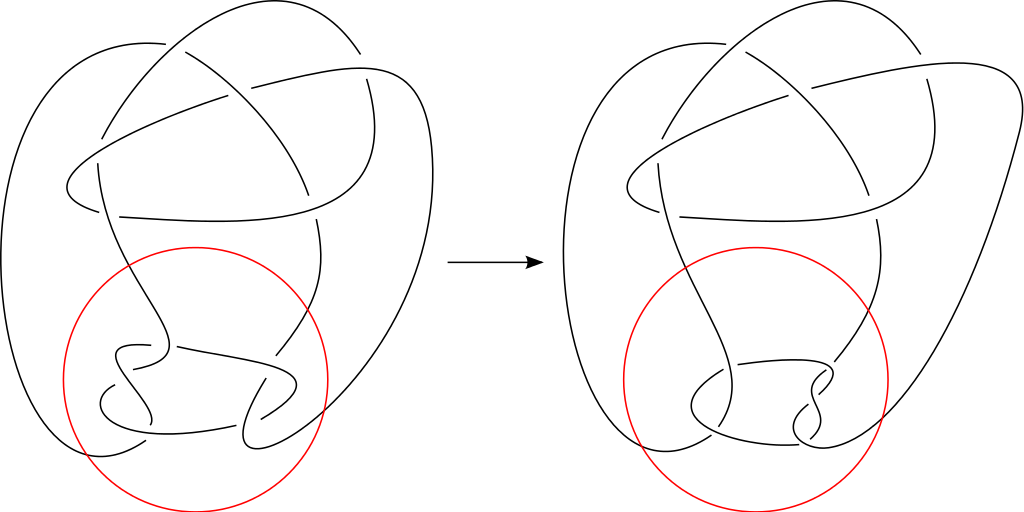
\includegraphics[width=0.601\linewidth]{../data/mixed/knudemutation.png}
    \caption{Węzły $11n_{42}$ oraz $11n_{34}$. Grafika Sørena Jørgensena, dostępna na licencji \href{https://creativecommons.org/licenses/by-sa/3.0/deed.en}{CC BY-SA 3.0} pod adresem \url{https://en.wikipedia.org/wiki/File:Knudemutation.svg}.}
\end{figure}
    
Niedawno Stojmenow podjął się systematycznie szukania mutantów wśród węzłów o~mniej niż 19 skrzyżowaniach (praca \cite{stoimenow2010} z~2010 roku).
\index[persons]{Stojmenow, Aleksander}%
Początkowo pracował sam, badając pewne subtelne przykłady postanowił uwikłać w swój projekt Toshifumiego Tanakę, a później także Daniela Mateię.
\index[persons]{Tanaka, Toshifumi}%
\index[persons]{Daniel, Matei}%
Praca \cite{stoimenow2010} jest kontynuacją artykułu, który napisali wspólnymi siłami.

I tak na stronie 531 można przeczytać, że ,,niezmienniki Wasiljewa co najwyżej 8. stopnia nie rozróżniają mutantów węzłów \cite{chmutov1994}'', ja tego nie widzę.
\index{niezmiennik!Wasiljewa}%
Mniej więcej sześć lat później wynik poprawił J. Murakami (nie mylić z H. Murakamim!) do 10. stopnia w~niezindeksowanej pracy \cite{murakami1999}.
\index[persons]{Murakami, Jun}
W międzyczasie Cromwell, Morton znaleźli niezmiennik stopnia 11., który odróżnia węzły Conwaya oraz Kinoshity-Terasakiego; patrz \cite{cromwell1996}.
\index[persons]{Cromwell, Peter}%
\index[persons]{Morton, Hugh}%
% czy Murakami potwierdził wynik Cromwella, Mortona?

Mutant węzła złożonego także jest złożony, co więcej istnieje bijekcja między czynnikami w ich rozkładach na węzły pierwsze Ruberman -- \cite{ruberman1987}.
\index[persons]{Ruberman, Daniel}%
Dzięki temu możemy bez straty ogólności założyć, że badamy tylko węzły pierwsze, niestety wciąż nie jest znana ogólna procedura pozwalająca wyliczyć wszystkie mutanty danego węzła.

Zaraz po rewolucji, jaką w latach 80. wywołała relacja kłębiasta, Ewing napisał z~Millettem komputerowy program w~języku C, który wyjątkowo szybko znajdował wielomiany HOMFLY oraz Kauffmana zadanego węzła.
\index[persons]{Ewing, Bruce}%
\index[persons]{Millett, Kenneth}%
Nawet dziś program ten jest w stanie uporać się z węzłami, z którymi nie radzą sobie inne narzędzia.
Autorzy nie wiedzieli wtedy, że ktoś jeszcze będzie z nich korzystać w przyszłości, dlatego poczynili w kodzie liczne optymalizacje dla stacji roboczej Sun, jaką wtedy dysponowali.
Dzisiaj okazuje się, że dla węzłów o większej liczbie skrzyżowań program często kończy swoje działanie zrzutem pamięci, wpada w pętlę bez wyjścia albo zwraca niepoprawny wynik (składniki wielomianu Kauffmana są postaci $a^m z^n$, gdzie $m + n$ jest nieparzyste).
Stojmenow korzystał z tych programów podczas tablicowania mutantów.
Jak postępował?
\begin{enumerate}
    \item podzielił węzły na grupy o tej samej objętości, wielomianie Jonesa oraz Alexandera;
    \item w każdej z grup szukał ciągu mutacji pomiędzy diagramami minimalnymi;
    \item tam, gdzie nie udało się znaleźć mutantów, liczył 2-kablowy wielomian HOMFLY;
    \item jeśli wielomian był taki sam, szukał ciągu mutacji między nieminimalnymi diagramami do 18 skrzyżowań;
    \item wreszcie pozostałe grupy zostały potraktowane reprezentacjami grupy podstawowej dwukrotnego nakrycia.
\end{enumerate}

Podsumowanie jego pracy zawiera tabela:

\begin{table}[H]
    \centering
    \begin{tabular}{lccccc} \toprule
        skrzyżowania & 11 & 12 & 13  & 14   & 15    \\ \midrule
        pary         & 16 & 70 & 703 & 3917 & 24884 \\
        trójki       &    & 5  & 38  & 233  & 1000  \\
        czwórki      &    &    & 32  & 262  & 2909  \\
        szóstki      &    &    & 1   & 17   & 172   \\
        ósemki       &    &    &     & 6    & 84    \\
        łącznie      & 16 & 75 & 774 & 4435 & 29049 \\
        \bottomrule
        \hline
    \end{tabular}
    \caption{Liczba grup mutantów wśród pierwszych węzłów do 15 skrzyżowań}
\end{table}

\subsubsection{Rozróżnianie mutantów}
Żaden wielomianowy niezmiennik opisany w~tej książce nie potrafi odróżnić od siebie węzłów $11n_{34}$ oraz $11n_{42}$.
Okazuje się, że niewielomianowe niezmienniki też często są bezradne.

\begin{proposition}
    Mutacja węzła nie zmienia jego wielomianu Alexandera.
\index{wielomian!Alexandera}%
\end{proposition}

% w commicie 1fe48ad183cb592e897f4151f9c18439baa84274 wymieniam:
% +    kablowego wielomianu Jonesa, % menasco91
% +    2-kablowego wielomianu HOMFLY, % przytycki89
% +    kablowego wielomianu Kauffmana, % lipson87
% +    sygnatury Tristrama-Levine'a, % cooper99
% +    symplicjalnEj objętości Gromowa, % ruberman87
% +    instanton homologii Floera, % ruberman99
% +    niezmienników Wittena % rong94
% +    ani Cassona. % kirk89
% ale teraz nie potrafię sobie przypomnieć, jak znalazłem te niezmienniki/prace. :(
% wydaje mi się, że źródłem nie jest stoimenow10, może Math Overflow?

\begin{proof}
    Stojmenow, Tanaka \cite[s. 1]{tanaka2009} piszą, że to proste ćwiczenie teorii kłębiastej, oraz że rozumowanie łatwo przenosi się na odkryte później wielomiany Jonesa, HOMFLY, BLM/Ho, Kauffmana.
\end{proof}

Warto przytoczyć teraz obserwację 3.8.2 z \cite[s. 43]{kawauchi1996} pochodzącą tak naprawdę z pracy Viro \cite{viro1973}: niech sploty $L_1, L_2$ będą mutantami, wtedy podwójne przestrzenie nakryciowe nad $S^3$ rozgałęzione wzdłuż $L_1$ albo $L_2$ są homeomorficzne z zachowaniem orientacji.
Cooper \cite{cooper1982} zauważył, że macierze Seiferta mutantów są $S$-równoważne.
\index{macierz!Seiferta}%
To tłumaczy czemu większość niezmienników nie radzi sobie z odróżnianiem mutantów.
% Viro: Two-fold branched coverings of three-sphere

% z tanaka09
Wzór kablowy\footnote{Niech $T$ będzie trywialnym torusem, zawierającym węzeł $K$, zaś $e \colon T \to S^3$ włożeniem $T$ na otoczenie węzła $C$ tak, że $e$ przenosi równoleżnik $T$ na równoleżnik $C$. Wtedy $\alexander_{eK} (t) = \alexander_K(t)\alexander_C(t^n)$.} \cite[tw. 6.15]{lickorish1997} pokazuje, że wielomian Alexandera nie odróżnia satelitów zmutowanych węzłów.
Wielomian Jonesa nie spełnia żadnego wzoru kablowego (gdyż czasami odróżnia kable węzłów o~tym samym wielomianie), ale…
\index{wzór!kablowy}%

\begin{proposition}
    Mutacja węzła nie zmienia jego kablowego wielomianu Jonesa.
\index{wielomian!Jonesa}%
\end{proposition}

\begin{proof}
\index[persons]{Morton, Hugh}%
\index[persons]{Traczyk, Paweł}%
    Morton, Traczyk \cite{traczyk1988}.
    % kiedyś tu było niezdefiniowane menasco91 = Menasco, Thistlethwaite: The Tait flyping conjecture, ale w 2022 roku przeczytałem Stoimenow: Tabulating and distinguishing mutants zmieniłem zdanie: "nonetheless Morton and Traczyk [36] showed that..."
\end{proof}

Praca \cite{traczyk1988} wspomina jeszcze, że to samo jest prawdą także dla ,,wielomianu Jonesa dwóch zmiennych'' (HOMFLY) i 2-kabli, ale nie dla dowolnych satelitów.
Fakt, że wielomian HOMFLY (a także Kauffmana) nie odróżniają 2-satelitów mutantów, odkryto rok wcześniej:

\begin{proposition}
\label{mutants_and_homfly}%
\index{wielomian!HOMFLY}%
    Mutacja węzła nie zmienia jego 2-kablowego wielomianu HOMFLY.
\end{proposition}

\begin{proof}
\index[persons]{Lickorish, William}%
\index[persons]{Lipson, Andrew}%
\index[persons]{Przytycki, Józef}%
    Lickorish, Lipson \cite{lipson1987}, później też Przytycki \cite{przytycki1989}.
    % TODO: skąd to o Przytyckim???
\end{proof}

Lepiej jest z~3-kablami: wielomian HOMFLY odróżnia tak węzły Kinoshity-Terasakiego i~Conwaya, ale wymaga takiej ilości rachunków, że mało komu chce się je przeprowadzać dla innych węzłów.
\index{węzeł!Conwaya}%
\index{węzeł!Kinoshity-Terasakiego}%

\begin{proposition}
    Mutacja węzła nie zmienia jego (2-?)kablowego wielomianu Kauffmana.
\index{wielomian!kablowy}%
\index{wielomian!Kauffmana}%
\end{proposition}

\begin{proof}
\index[persons]{Lickorish, William}%
\index[persons]{Lipson, Andrew}%
    Lickorish, Lipson \cite{lipson1987}.
\end{proof}

Morton w recenzji pracy Lickorisha, Lipsona wspomina, że dla satelitów owijających się więcej niż $2$ razy to nie jest prawda, jak później odkryto.

\begin{proposition}
\index{wielomian!BLM/Ho}%
    Mutacja węzła nie zmienia jego wielomianu BLM/Ho.
\end{proposition}

\begin{proof}
    \cite{tanaka2009}, choć nie wiemy, gdzie dokładnie.
\end{proof}

\begin{proposition}
\index{sygnatura!Levine'a-Tristrama}%
    Mutacja węzła nie zmienia jego sygnatury Levine'a-Tristrama.
\end{proposition}

\begin{proof}
\index[persons]{Cooper, Daryl}%
\index[persons]{Lickorish, William}%
    Cooper, Lickorish w~\cite{cooper1999} podają klasyczny dowód, że mutacja zachowuje wielomian Alexandera, oparty o~macierz Seiferta.
    Wiedząc, jak wygląda ta macierz, autorzy wyciągają wniosek, że sygnatura splotów (!) w~homologicznej 3-sferze też jest zachowywana.
\end{proof}

\begin{proposition}
\index{objętość!symplicjalna Gromowa}%
\label{mutants_the_same_volume}%
    Mutacja węzła nie zmienia jego symplicjalnej objętości Gromowa.
\end{proposition}

\begin{proof}
\index[persons]{Ruberman, Daniel}%
    Ruberman \cite{ruberman1987}.
    % Ruberman [42] showed that mutants have equal volume in all hyperbolic pieces of the JSJ decomposition.
\end{proof}

\begin{proposition}
\index{homologia!Floera}%
    Mutacja węzła nie zmienia jego instanton homologii Floera.
\end{proposition}

\begin{proof}
\index[persons]{Ruberman, Daniel}%
    Jeszcze raz Ruberman \cite{ruberman1999}.
\end{proof}

\begin{proposition}
\index{niezmiennik!Wittena}%
    Mutacja węzła nie zmienia jego niezmienników Wittena.
\end{proposition}

\begin{proof}[Niedowód]
    Rong \cite{rong1994}: niech $L$ będzie obramowanym splotem w~3-rozmaitości $M$, zaś $F \subseteq M$ dwustronną powierzchnią, tnącą splot w 0, 1 lub 4 (transwersalnie) punktach, o genusie $g = 0$, $1$ lub $2$, wtedy rozcięcie $M$ wzdłuż $F$ i sklejenie po obrocie o 180 stopni daje parę $(M^\tau, K^\tau)$, która ma ten sam niezmiennik Wittena w $\mathrm{SU}(2)$ jak wyjściowa para $(M, K)$.
    % TODO: dla wybranych mutacji
\end{proof}

\begin{proposition}
\index{niezmiennik!Cassona}%
    Mutacja węzła nie zmienia jego niezmienników Cassona.
\end{proposition}

Celowo nie podajemy definicji tego niezmiennika.
Nieformalnie, zlicza on co drugą klasę sprzężoności reprezentacji grupy podstawowej homologicznej 3-sfery w grupie $SU(2)$.

\begin{proof}
\index[persons]{Kirk, Paul}%
    Kirk \cite{kirk1989}.
\end{proof}

\begin{conjecture}
    Mutacja węzła nie zmienia jego liczby gordyjskiej.
\end{conjecture}

Jak czytamy w \cite[problem 1.69]{kirby1978}, przypuszczenie to jest bardzo trudne do udowodnienia, bo wynikałaby z niego bardzo stara hipoteza \ref{conjecture_unknotting_additive}, że liczba gordyjska splotów jest addytywna.
\index{hipoteza!o liczbie gordyjskiej}%
Przytoczymy dwa częściowe wyniki.
Najpierw Rolfsen \cite{rolfsen1993} zauważył, że jedynym mutantem niewęzła jest sam niewęzeł.
\index[persons]{Rolfsen, Dale}%
Dekadę później Gordon, Luecke \cite{gordon2006} pokazali, iż klasa węzłów $1$-gordyjskich jest zamknięta na przeprowadzanie mutacji.
\index[persons]{Gordon, Cameron}%
\index[persons]{Luecke, John}%
(Ohtsuki \cite[problem 12.15]{ohtsuki2002} powtarza hipotezę.)
\index[persons]{Ohtsuki, Tomotada}%

% to NIE jest z stoimenow10
\begin{proposition}
    Niech $D$ będzie alternującym diagramem.
    Wtedy każdy mutant $D$ też jest alternujący.
\end{proposition}

Wśród niezmienników, które mutacja czasami zmienia, znajduje się genus plastrowy:

\begin{proposition}
\index{genus!plastrowy}%
    Niech $m, n$ będą nieujemnymi liczbami całkowitymi.
    Wtedy istnieje węzeł $K$ o genusie plastrowym równym $m$, którego pewien mutant ma genus plastrowy równy $n$.
\end{proposition}

Stanowi to uogólnienie obserwacji Livingstona \cite{livingston1983}, że istnieją mutanty o~różnym genusie plastrowym.
\index[persons]{Livingston, Charles}%

\begin{proof}
    Kim, Livingston w \cite{kim2005}.
\end{proof}

Zbiór problemów niskowymiarowej topologii opublikowany przez Kirby'ego \cite{kirby1978} zawiera następujące pytanie:
\index[persons]{Kirby, Rob}%

\begin{conjecture}[problem 1.91]
\index{węzeł!satelitarny}
    Niech $K$ będzie prostym węzłem bez orientacji (w jego dopełnieniu nie ma nierównoległych do brzegu, nieściśliwych pierścieni).
\index{nieściśliwy}%
    Czy istnieją węzły niebędące mutantami $K$, których nie można odróżnić od $K$ wielomianem Jonesa oraz wszystkimi jego satelitami?
\end{conjecture}

Stojmenow pisze, że tak: pierwszą chronologicznie parą jest $14_{41721}$, $14_{42125}$, dowód opiera się na wzorze fuzyjnym Masbauma-Vogela z~pracy \cite{masbaum1994}.
\index[persons]{Stojmenow, Aleksander}
\index[persons]{Masbaum, Gregor}%
\index[persons]{Vogel, Pierre}%
\index{wzór!fuzyjny Masbauma-Vogela}%
Patrz \cite[przykład 3.3]{tanaka2009} oraz \cite[przykład 3.2]{stoimenow2010}.

Choć wzór ten zastosowany do konkretnej pary węzłów sprawia zazwyczaj trudności rachunkowe, to jest wystarczającym narzędziem, by rozszerzyć konstrukcję do ogólnego wyniku:

\begin{proposition}
    Istnieje nieskończenie wiele par prostych węzłów hiperbolicznych o tych samych kolorowych wielomianach Jonesa, które nie są swoimi mutantami.
\end{proposition}

\begin{proof}
    Stojmenow, Tanaka \cite[tw. 1.1]{tanaka2009}.
\end{proof}

\index{mutant|)}




\section{Precle}
\index{węzeł!preclowy|see {precel}}%
\index{precel|(}%
Precle to sploty ze standardowym diagramem, na którym wyróżnić można co najmniej trzy warkocze na dokładnie dwóch pasmach.
Warkocze te ułożone są w sposób cykliczny.
Pojawiły się po raz pierwszy w~książce Reidemeistera z~1932 roku jako przykład węzła o~trywialnym wielomianie Alexandera.
Zanim podamy formalną definicję, wygodnie będzie przyjrzyć się ogólniejszej rodzinie splotów Montesinosa, nazwanych tak na cześć José Marii Montesinosa Amilibii, topologa hiszpańskiego.
\index[persons]{Montesinos, José}%
Wprowadził je do matematyki w~1973 roku \cite{montesinos73}.

Kawauchi \cite[s. 29]{kawauchi96} pisze, że Montesinos uogólnił precle, bo dwukrotne nakrycie nad $S^3$ rozgałęzione wzdłuż precla jest rozmaitością Seiferta.
\index{rozmaitość Seiferta}%

\index{splot!Montesinosa|(}%
\begin{definition}[splot Montesinosa]
    Splotem Montesinosa nazywamy splot o~poniższym diagramie, gdzie wymierne liczby $\alpha_i/\beta_i$ oraz całkowita $e \in \Z$ odpowiadają supłom.
\begin{comment}
    \[
    \begin{tikzpicture}[baseline=-0.65ex, scale=0.1]
    %\useasboundingbox (-5, -9) rectangle (5, 5);
        \draw[semithick] (-5, 5) rectangle (5, 15);
        \foreach \x in {0,1,3,4} {
            \draw[semithick] (15*\x-35, -15) rectangle (15*\x-25, -5);
        }
        \foreach \x in {0,1,2,3,4,5} {
            \draw[semithick] (15*\x-35, -8) to (15*\x-40, -8);
            \draw[semithick] (15*\x-35, -12) to (15*\x-40, -12);
        }
        \draw[semithick] (-40, -8) [in=down, out=left] to (-45, -3);
        \draw[semithick] (-40, -12) [in=down, out=left] to (-49, -3);

        \draw[semithick] (-40, 8) [in=up, out=left] to (-45, 3);
        \draw[semithick] (-40, 12) [in=up, out=left] to (-49, 3);

        \draw[semithick] (40, 8) [in=up, out=right] to (45, 3);
        \draw[semithick] (40, 12) [in=up, out=right] to (49, 3);

        \draw[semithick] (40, -8) [in=down, out=right] to (45, -3);
        \draw[semithick] (40, -12) [in=down, out=right] to (49, -3);

        \draw[semithick] (-45, -3)  to (-45, 3);
        \draw[semithick] (-49, -3)  to (-49, 3);
        \draw[semithick] (45, -3)  to (45, 3);
        \draw[semithick] (49, -3)  to (49, 3);

        \draw[semithick] (-5, 8)  to (-40, 8);
        \draw[semithick] ( 5, 8)  to ( 40, 8);
        \draw[semithick] (-5, 12)  to (-40, 12);
        \draw[semithick] ( 5, 12)  to ( 40, 12);

        \node at (0, 10) {e};
        \node at (0, -10) {\ldots};
        \node at (-15, -10) {$\displaystyle \frac{\alpha_2}{\beta_2}$};
        \node at (-30, -10) {$\displaystyle \frac{\alpha_1}{\beta_1}$};
        \node at (15, -10) {$\displaystyle \frac{\alpha_{n-1}}{\beta_{n-1}}$};
        \node at (30, -10) {$\displaystyle \frac{\alpha_n}{\beta_n}$};
    \end{tikzpicture}
    \]
\end{comment}
\end{definition}

Cały dwunasty rozdział podręcznika Burdego i~Zieschanga \cite{burde14} jest poświęcony splotom Montesinosa.
Można tam znaleźć ich klasyfikację, zawiera jednak pułapkę: autorzy używają innej notacji dla supłów dwumostowych.
Podają przykład węzła $43/105 = [0, 2, 2, 3, 1, 4]$, dla nas to jest $105/22 = [4, 1, 3, 2, 2]$.

\begin{proposition}
    Sploty Montesinosa o $r \ge 3$ supłach $\beta_1/\alpha_1, \beta_2/\alpha_2, \ldots$ takich, że
    \begin{equation}
        \sum_{j=1}^r \frac{1}{\alpha_j} \le r - 2
    \end{equation}
    są sklasyfikowane (z dokładnością do cyklicznych permutacji oraz odwracania) przez uporządkowany zbior ułamków $\{\beta_i/\alpha_i \mod 1 : 1 \le i \le r\}$ razem z~wymierną liczbą
    \begin{equation}
        e_0 = e + \sum_{j=1}^r \frac{\beta_j}{\alpha_j}.
    \end{equation}
\end{proposition}

Powyższy fakt nie używa naszej notacji!

\begin{proof}
\index[persons]{Bonahon, Francis}%
    Praca doktorska Bonahona \cite{bonahon79}.
    W~internecie dostępny jest jej skan (gdyż była pisana odręcznie po francusku!), ale angielskie tłumaczenie nie istnieje.
\end{proof}

Używając nadal tej niestandardowej notacji można sklasyfikować węzły odwracalny czy zwierciadlane:

\begin{proposition}
\index{węzeł!zwierciadlany}%
    Splot Montesinosa jest zwierciadlany wtedy i tylko wtedy, gdy $e = 0$ oraz istnieje permutacja $\pi$, cykl długości $r$ lub odwrócenie, taka że
    \begin{equation}
        \frac{\beta_{\pi(i)}}{\alpha_{\pi(i)}} \equiv -\frac{\beta_i}{\alpha_i} \pmod 1
    \end{equation}
\end{proposition}

\begin{proof}
    Burde, Zieschang, Heusener \cite[s. 230]{burde14}.
\end{proof}

\begin{corollary}
    Splot Montesinosa z nieparzystą liczbą supłów nie jest zwierciadlany.
\end{corollary}

\begin{proposition}
\index{węzeł!odwracalny}%
    Splot Montesinosa jest odwracalny wtedy i tylko wtedy, gdy, po ewentualnej zmianie etykiet supłów, przynajmniej jedna z liczb $\alpha_i$ jest parzysta lub wszystkie liczby $\alpha_i$ są parzyste, a sam splot ma postać
    \begin{equation}
        M(e_0, \beta_1/\alpha_1, \ldots, \beta_p/\alpha_p, \beta_p/\alpha_p, \ldots, \beta_1/\alpha_1)
    \end{equation}
    (oraz $r = 2p$) lub
    \begin{equation}
        M(e_0, \beta_1/\alpha_1, \ldots, \beta_p/\alpha_p, \beta_{p+1}/\alpha_{p+1}, \beta_p/\alpha_p, \ldots, \beta_1/\alpha_1)
    \end{equation}
    (oraz $r = 2p+1$) lub
    \begin{equation}
         M(e_0, \beta_1/\alpha_1, \ldots, \beta_p/\alpha_p, \beta_{p+1}/\alpha_{p+1}, \beta_p/\alpha_p, \ldots, \beta_2/\alpha_2).
    \end{equation}
    (oraz $r = 2p$).
\end{proposition}

\begin{proof}
    Burde, Zieschang, Heusener \cite[s. 231]{burde14}.
\end{proof}

\index{splot!Montesinosa|)}%

% DICTIONARY;pretzel;preclowy;węzeł
\begin{definition}[precel]
\label{def:pretzel}%
    Splot Montesinosa o~całkowitych współczynnikach nazywamy preclem.
\end{definition}

Na standardowym diagramie precla $(p_1, p_2, \ldots, p_n)$ występuje $p_1$ lewych skrzyżowań w~pierwszym suple, $p_2$ w~drugim, i~tak dalej.
Taki precel jest węzłem dokładnie wtedy, gdy $n$ oraz $p_i$ są nieparzyste lub dokładnie jedna z~liczb $p_i$ jest parzysta (\cite[s. 27]{kawauchi96}).

\begin{proposition}
    Jeśli co najmniej dwa współczynniki $p_i, p_j$ zerują się, precel jest rozszczepialny.
\end{proposition}

\begin{proof}
    Widać to bezpośrednio z diagramu: jego część zawarta między supłem $p_i$ oraz $p_j$ jest rozłączna z~resztą diagramu.
    Nie jest jednak prawdziwa implikacja odwrotna.
    % TODO: podać przykład
\end{proof}

Precel $(1,1,1)$ to prawy trójlistnik, $(5, -1, -1)$ to węzeł dokerski $6_1$, $(-3, 0, -3)$ to splot dwóch trójlistników, zaś $(2p, 2q, 2r)$ jest splotem trzech niewęzłów.
Precle $(-2, 3, 2n+1)$ są szczególnie użyteczne jako narzędzie do badania 3-rozmaitości.
Wiele twierdzeń, które dotyczą takich rozmaitości, opiera się na przykład na chirurgii Dehna precla $(-2, 3, 7)$.
\index{chirurgia Dehna}%
\index{precel!(-2, 3, 7)}%

\begin{proposition}
\index{węzeł!torusowy}%
    Niech $K$ będzie węzłem torusowym.
    Jeśli $K$ jest jednocześnie $(-2, 3, k)$-preclem, to
    \begin{equation}
        K = 5_{1} = T_{2,5} = P(1, 3, -2)
    \end{equation}
    albo
    \begin{equation}
        K = 8_{19} = T_{3,4} = P(3, 3, -2)
    \end{equation}
    albo
    \begin{equation}
        K = 10_{124} = T_{3,5} = P(5, 3, -2).
    \end{equation}
\end{proposition}

\begin{proof}
\index[persons]{Garoufalidis, Stavros}%
\index[persons]{Koutschan, Christoph}%
    Garoufalidis, Koutschan \cite{garoufalidis12}.
\end{proof}

\begin{proposition}
    \label{prp:pretzel_not_invertible}
    Niech $p, q, r$ będą liczbami nieparzystymi takimi, że $|p|, |q|, |r|$ są parami różne i większe niż $1$.
    Wtedy $(p, q, r)$-precel jest nieodwracalny.
\end{proposition}

\begin{proof}
\index[persons]{Fox, Ralph}%
\index[persons]{Trotter, Hale}%
    Zgodnie z sugestią Foxa, Trotter przetłumaczył problem na język teorii grup w \cite{trotter63}.
    Wyróżnia w~grupie węzła dwa elementy -- (zorientowany) południk i równoleżnik.
    Jeśli dwa węzły są równoważne, to homeomorfizm $\R^3 \to \R^3$ posyłający jeden na drugi wyznacza izomorfizm ich grup podstawowych, który posyła południk na południk i równoleżnik na równoleżnik.
    W szczególności, jeśli węzeł jest odwracalny, to jego grupa posiada specjalny automorfizm (,,inwersję'') odwracający zarówno południk, jak i równoleżnik.
    To prowadzi do sprzeczności w przypadku rozpatrywanych precli.
\end{proof}

Wystarczający warunek z tego stwierdzenia jest prawie konieczny.
Jeśli $p = r$, węzeł można odwrócić przez półobrót wokół środkowej osi.
Cykliczne permutacje trójki $(p, q, r)$ nie zmieniają węzła, więc wszystkie trzy liczby $p, q, r$ muszą być różne.
Jeśli jedna z tych liczb jest parzysta, półobrót wokół poziomej osi odwraca węzeł.
Z pracy Bankwitza i Schumanna wynika, że jeśli któryś z parametrów ma wartość $\pm 1$, to węzeł też jest odwracalny.
\index[persons]{Bankwitz, Carl}%
\index[persons]{Schumann, Hans}%
% Bankwitz, Carl; Schumann, Hans Georg;
% Über viergeflechte. (German)
% Abh. Math. Sem. Univ. Hamburg 10 (1934), no. 1, 263–284.
Nie jest trudno pokazać to wprost.
Zatem nie wiemy jedynie jakie są precle $(p, q, -q)$, gdzie $|p| \neq |q|$ oraz $|p|, |q| \ge 3$.

Jeśli liczby $p, q, r$ są nieparzyste i tego samego znaku, to wyznacznik precla $(p, q, r)$ jest postaci $4n+3$.
\index{wyznacznik}%
Wtedy używając formy kwadratowej (jak Reidemeister w 1932!) można pokazać, że taki węzeł nie jest achiralny.
Niech $K$ będzie zorientowanym preclem $(3, 5, 7)$.
Wtedy $K$, $mK$, $rK$, $mrK$ są parami nierównoważne.
Węzeł $K \shrap mK$ jest dodatnio zwierciadlany, zaś $rK \shrap mK$ ujemnie zwierciadlany.
Trójlistnik jest odwracalny, ale nie zwierciadlany, ósemka jest zwierciadlana i~odwracalna.
To pokazuje, że wszystkie typy symetrii są realizowane przez precle lub sumy precli.

\begin{proposition}
\label{prp:pretzel_alexander}%
\index{wielomian!Alexandera}%
    Jeżeli liczby $p, q, r$ są nieprzyste, to wielomianem Alexandera $(p, q, r)$-precla jest
    \begin{equation}
        \alexander = \frac 14 ((pq+qr+pr) (t-1)^2 + (t+1)^2).
    \end{equation}
\end{proposition}

\begin{proof}
\index[persons]{Bae, Yongju}%
\index[persons]{Lee, In}%
    Bae, Lee pokazali w \cite[lemat 3.1]{bae20}, że macierz Seiferta $(p, q, r)$-precla to
    \begin{equation}
        M = \frac 1 2 \begin{bmatrix}
            p+q & p-1 \\
            p+1 & p+r
        \end{bmatrix},
    \end{equation}
    wystarczy więc użyć wzoru $\alexander = \det(M-tM^t)$.
\end{proof}

Wielomian Alexandera precla $(p_1, \ldots, p_n)$ nigdy nie zależy od kolejności współczynników, jest to ćwiczenie w~książce Livingstona \cite[s. 215]{livingston93}.

\begin{proposition}
\index{kolorowalność}%
    Niech $n$ będzie liczbą pierwszą.
    Węzeł $p, q, r$-preclowy jest $n$-kolorowalny wtedy i~tylko wtedy, gdy $n$ dzieli $|pq+qr+pr|$.
    Jeśli przynajmniej jedna z~liczba $p, q, r$ nie jest wielokrotnością $n$, kolorowanie z dokładnością do permutacji jest jedyne.
    W przeciwnym przypadku istnieją cztery różne kolorowania.
\end{proposition}

\begin{proof}
\index[persons]{Brownell, Kathryn}%
\index[persons]{O'Neil, Kaitlyn}%
\index[persons]{Taalman, Laura}%
    Pierwsza część jest wnioskiem ze stwierdzeeń \ref{prp:colour_determinant}, \ref{prp:alexander_determinant} oraz \ref{prp:pretzel_alexander}.
    Dowód drugiej zawiera praca Brownell, O'Neil, Taalman \cite{taalman05}, trzech Amerykanek.
\end{proof}

Podano tam także ogólny wzór na liczbę $n$-kolorowań dowolnego węzła.

\index{precel|)}%

% Koniec sekcji Precle



\section{Węzły Lissajous}
% szkielet: praca Lamma
\index{węzeł!Lissajous|(}%
Węzły Lissajous zdefiniowali Bogle, Hearst, Jones i Stoiłow \cite{bogle94} jako węzły, których pewien diagram jest krzywą Lissajous.

\begin{definition}[węzeł Lissajous]
    Węzeł zadany parametrycznie:
    \begin{equation}
        x = \cos(n_xt + \varphi_x) \quad
        y = \cos(n_yt + \varphi_y) \quad
        z = \cos(n_zt + \varphi_z),
    \end{equation}
    gdzie $n_x, n_y, n_z$ (,,częstotliwości'') to stałe całkowite, zaś $\varphi_x, \varphi_y, \varphi_z$ (,,fazy'') są rzeczywiste, nazywamy węzłem Lissajous.
\end{definition}

Węzeł nie może posiadać samoprzecięć, dlatego żadna z~wielkości $n_i\varphi_j-n_j\varphi_i$, dla różnych indeksów $i, j$ nie może być krotnością $\pi$.
Bez straty ogólności możemy założyć, że $\varphi_z = 0$.
Dodatkowo stałe $n_x, n_y, n_z$ muszą być parami względnie pierwsze.

Wiele węzłów jest węzłami Lissajous:

\begin{example}
    Dla $n_x = 3$, $n_y = 2$, $n_z = 7$, $\varphi_x = 7/10$, $\varphi_y = 2/10$ mamy węzeł $5_2$.
\end{example}

\begin{example}
    Węzły pierwsze $6_1$, $7_4$, $8_{15}$, $10_1$, $10_{35}$, $10_{58}$ są węzłami Lissajous.
\end{example}

\begin{example}
    Suma prawego i~lewego trójlistnika, suma dwóch kopii $5_2$ są węzłami Lissajous.
\end{example}

Jest wiele węzłów Lissajous:

\begin{proposition}
    Istnieje nieskończenie wiele węzłów Lissajous.
\end{proposition}

\begin{proof}
    Niech $a, b > 1$ będą względnie pierwsze.
    Lamm w \cite{lamm97} pokazał dużo ogólniejszy wynik.
    Mianowicie: węzeł Lissajous o~częstotliwościach $n_x = a$, $n_y = b$, $n_z = 2ab-a-b$ oraz fazach:
    \begin{equation}
        \varphi_x = \frac{2n_x-1}{n_z} \pi, \quad
        \varphi_y = \frac{\pi}{n_z}, \quad
        \varphi_z = 0
    \end{equation}
\index{sygnatura}%
\index{genus}%
    posiada sygnaturę $\sigma = a+b-ab-1$ i genus $g = -\sigma/2$.
\end{proof}

Węzły Lissajous są bardzo symetryczne.

\begin{proposition}
\index{węzeł!silnie dodatnio achiralny}
    Jeśli wszystkie stałe $n_x, n_y, n_z$ są nieparzyste, węzeł jest silnie dodatnio achiralny.
\end{proposition}

\begin{proposition}
\index{węzeł!okresowy}%
\label{prp:lissajous_two_periodic}%
    Jeśli jedna z częstotliwości jest parzysta, to węzeł jest 2-okresowy.
\end{proposition}

\begin{proof}
    Załóżmy, że częstotliwość $n_x$ jest parzysta.
    Wtedy półobrót wokół osi $x$ odwzorowuje węzeł w~siebie.
\end{proof}

To nakłada ograniczenia na wielomian Alexandera.

\begin{proposition}
\index{wielomian!Alexandera}
\label{prp:lissajous_alexander}%
    Niech $K$ będzie węzłem Lissajous.
    Wtedy $\alexander(x)$, jego wielomian Alexandera, jest kwadratem w~pierścieniu $(\Z/2\Z)[x]$.
\end{proposition}

\begin{proof}
    Rozpatrzmy dwa przypadki.

    Jeśli wszystkie częstotliwości są nieparzyste, węzeł jest silnie dodatnio achiralny.
    Wtedy wielomian $\alexander(x)$ jest kwadratem w pierścieniu $\Z[x]$ (pokazano to w \cite{hartley79}).

    W przeciwnym razie możemy powołać się na fakt \ref{prp:lissajous_two_periodic} oraz \ref{prp:murasugi_periodic} (z $n=2^1$ oraz $\lambda = 1$).
    Dostaniemy równość
    \begin{equation}
        \label{eqn:lissajous_squared}
        \alexander_K(t) \equiv \alexander^2_{J}(t) \mod 2,
    \end{equation}
    która kończy dowód.
\end{proof}

Warto zwrócić uwagę, że bycie silnie dodatnio achiralnym jest bardzo restrykcyjnym warunkiem.
Spośród pierwszych węzłów o~co najwyżej 12 skrzyżowaniach, tylko trzy go spełnia: 10a103 ($10_{99}$), 10a121 ($10_{123}$) oraz 12a427.
Tylko pierwszy z nich jest na pewno węzłem Lissajous (stan na 2018).

\begin{example}
    Trójlistnik oraz ósemka nie są węzłami Lissajous.
\end{example}

Wygodnie jest przeformułować warunek z faktu \ref{prp:lissajous_alexander} do następującej postaci.
Wielomian $\alexander(t) = A_0 + A_1(t+1/t) + \ldots + A_n(t^n + 1/t^n)$ jest kwadratem modulo $2$ wtedy i tylko wtedy, gdy współczynniki $A_{2k+1}$ są parzyste dla $k \ge 0$.

\begin{corollary}
\index{niezmiennik!Arfa}%
    Niech $K$ będzie węzłem Lissajous, wtedy niezmiennik $\operatorname{Arf} K = 0$ znika.
\end{corollary}

\begin{proof}
    Niech $\alexander(t) = A_0 + A_1(t+1/t) + \ldots + A_n(t^n + 1/t^n)$ będzie  wielomianem Alexandera.
    Wtedy $\alexander_K(1) = \pm 1$, zatem $0 = \pm 1 + A_0 + 2A_1 + \ldots + 2A_n$.
    Możemy teraz odjąć to od $\alexander_K(-1) = A_0 - 2A_1 \pm \ldots$, by uzyskać $\alexander_K(-1) = \pm 1 - 4A_1 - 4A_3 - \ldots$.
    Razem z wygodnym przeformułowaniem daje to $\alexander_K(-1) \equiv \pm 1 \mod 8$, co w połączeniu z~\ref{prp:arf_murasugi} kończy dowód.
\end{proof}

\begin{corollary}
\index{węzeł!włóknisty}%
\label{cor:lissajous_fibered}%
    Włókniste węzły o nieparzystym genusie nie są węzłami Lissajous.
\end{corollary}

%=% Lamm
\begin{proof}
    Wynika to z~naszego wygodnego przeformułowania oraz stwierdzenia 8.33 w książce \cite{burde14}: jeśli $K$ jest włóknistym węzłem o genusie $g$, to wielomian Alexandera $\alexander_K$ jest stopnia $2g$ i~ma wiodący współczynnik $\pm 1$.
\end{proof}

\begin{corollary}
\index{węzeł!dwumostowy}%
\label{cor:lissajous_twobridge}%
    Niech $K$ będzie dwumostowym węzłem Lissajous.
    Wtedy $\alexander_K(t) \equiv 1 \mod 2$.
\end{corollary}

\begin{proof}
    Nietrywialny węzeł o dwóch mostach nie może być silnie dodatnio achiralny (patrz \cite{hartley79}).
    Jeśli jest węzłem Lissajous, jedna z jego częstotliwości okazuje się być parzysta.
    Wtedy jego faktor jest trywialny i~kongruencja \ref{eqn:lissajous_squared} daje $\alexander_K(t) \equiv 1 \mod 2$.
\end{proof}

%=% Lamm
\begin{corollary}
\index{węzeł!włóknisty}%
    Dwumostowe węzły włókniste nie są węzłami Lissajous.
\end{corollary}

Można skorzystać z tego samego argumentu, co w dowodzie wniosku \ref{cor:lissajous_fibered} oraz \ref{cor:lissajous_twobridge}.

%=% Lamm
\begin{proposition}
    Niech $p, q$ będą względnie pierwszymi liczbami różnymi od $0, \pm 1$, zaś $K$ węzłem.
    Wtedy $(p, q)$-kabel węzła $K$ nie jest węzłem Lissajous.
\end{proposition}

Lamm pisze, że obiekt ten -- $(p, q)$-kabel -- zdefiniowano w książce Eisenbuda/Neumanna ,,Three-dimensional link theory and invariants of plane curve singularities''.
Celowo pomijamy ją w bibliografii, prawdopodobnie chodzi o zwykłe węzły satelitarne.

\begin{proof}
    Niech $L$ będzie $(p, q)$-kablem węzła $K$.
    Seifert pokazał w \cite{seifert50}, że
    \begin{equation}
        \alexander_L(t) = \frac{(t^{pq}-1)(t-1)}{(t^p-1)(t^q-1)} \alexander_K(t^p),
    \end{equation}
    przy czym wyjątkowo wielomian $\alexander$ nie jest symetryczny w $t$ oraz $1/t$, tylko unormowany.
    Dwa najwyższe współczynniki w wielomianie ,,ułamkowym'' to $\pm 1$, a skoro $|p| > 1$, dwa najwyższe współczynniki $\alexander_L$ to także $\pm 1$.
    ,,Wygodne sformułowanie'' kończy dowód.
\end{proof}

\begin{corollary}
\index{węzeł!torusowy}%
    Nietrywialne węzły torusowe nie są węzłami Lissajous.
\end{corollary}

\begin{proof}
    Węzły torusowe to kable niewęzła.
\end{proof}

\begin{corollary}
    Nietrywialne węzły algebraiczne nie są węzłami Lissajous.
\end{corollary}

Co to są węzły algebraiczne?
Nie wiem.

\begin{proof}
    Wynika to z ogólniejszego stwierdzenia: jeśli spełniony jest warunek $|p_n|, |q_n| > 1$, to iterowane węzły torusowe typu $((p_n, q_n), (p_1, q_1))$ nie są węzłami Lissajous.
\end{proof}

Podamy teraz pierwszy warunek wystarczający, by być węzłem Lissajous.
Znaleźli go Hoste z Zirbel w~\cite{zirbel06}:

\begin{proposition}
\index{niezmiennik!Arfa}%
\index{węzeł!skręcony}%
    Niech $K$ będzie węzłem skręconym.
    Następujące warunki są równoważne: $K$ jest węzłem Lissajous; niezmiennik Arfa węzła $K$ znika.
\end{proposition}

Węzły bilardowe to zamknięte trajektorie kuli, która zostaje wystrzelona z jednej ze ścian sześcianu, odbija się pod takim samym kątem, pod jakim pada na ściany.
\index{węzeł!bilardowy}%
Jones, Przytycki pokazali w~\cite{jones98}, że węzły bilardowe to dokładnie węzły Lissajous i~zadali pytanie, czy każdy węzeł można zrealizować jako trajektorię kuli w~jakimś wielościanie.

Odpowiedź jest pozytywna.
Koseleff, Pecker w~\cite{koseleff14} korzystając z~twierdzenia Manturowa
\index{twierdzenie!Manturowa (o kwazitorycznych warkoczach)}%
(każdy splot jest domknięciem kwazitorycznego warkocza)
pokazują, że każdy węzeł ma diagram, który jest wielokątem gwiaździstym.
Użyte zostało twierdzenie Kroneckera z~1884 roku: jeśli liczby $\theta_0 = 1, \theta_1, \ldots, \theta_k$ są liniowo niezależne nad ciałem $\Q$, to zbiór punktów $(\lfloor n\theta_i \rfloor_{i=0}^k)_{n=0}^\infty$ leży gęsto w kostce jednostkowej.

Lamm, Obermeyer dowiedli w 1999, że węzły bilardowe wewnątrz walca są taśmowe albo okresowe, więc w walcu nie można zrealizować każdego węzła.
\index{węzeł!okresowy}%
\index{węzeł!taśmowy}%
Lamm postawił hipotezę, że jest to możliwe w eliptycznym walcu.
Pozytywnej odpowiedzi ponownie udzielił niedawno Pecker w \cite{pecker12}.

\index{węzeł!Lissajous|)}

% Koniec sekcji Węzły Lissajous


\section{Węzły torusowe} % (fold)
\label{sec:torus}
W tej sekcji przyjrzymy się węzłom o specjalnym ułożeniu w przestrzeni $\R^3$.
Do ich określenia potrzebny jest torus trywialny,
powierzchnia otrzymana przez obrót okręgu $(x-2)^2 + y^2 = 1$ wokół osi $y$.
Można go także uzyskać przez sklejenie podstaw walca tak, by go przy tym nie zapętlić.
Oczywiście istnieją też nietrywialne torusy, na przykład rurowe otoczenie trójlistnika.

\begin{definition}
    \index{węzeł!torusowy}
    Węzeł (splot) torusowy to taki, który leży na powierzchni niezaplątanego torusa.
\end{definition}

Na walcu $S^2 \times [0,1]$, którego podstawa leży w płaszczyźnie $xy$, rozpatrzmy $r$ skierowanych odcinkach (dla $k = 0, 1, \ldots, r - 1$) o końcach w punktach
\begin{align*}
    \left(\cos \frac{2k \pi}{r}, \sin \frac{2k\pi}{r}, 0 \right), \quad
    \left(\cos \frac{2k \pi}{r}, \sin \frac{2k\pi}{r}, 1 \right).
\end{align*}
Przekręćmy górną podstawę walca wokół osi $z$ o skierowany kąt $2\pi q / r$ oraz utożsammy ze sobą pary punktów $(x, y, 0) \sim (x, y, 1)$,
Uzyskaliśmy splot torusowy $K_{q, r}$: okrąża on $q$ razy rdzeń torusa i $p$ razy jego oś symetrii obrotowej.
Określimy jeszcze kilka splotów torusowych.
Węzeł $K_{0, 0}$ leży na powierzchni torusa i jest ściągalny do punktu, zaś $K_{1, 0}$ to nawinięta toroidalnie pętla.
Węzeł $K_{p, q}$ posiada następującą parametryzację:
\[
    x = (2+\cos q \phi) \cos p \phi, \quad
    y = (2+\cos q \phi) \sin p \phi, \quad
    z = - \sin q \phi, \quad
    0 \le \phi \le 2\pi.
\]
Poniżej przedstawiamy trzy węzły torusowe.

\begin{figure}[H]
    \begin{minipage}[b]{.3\linewidth}
        \centering
        
\includegraphics[width=\linewidth]{../data/torus-p2-q3.pdf}
        \subcaption{trójlistnik: $p = 2, q = 3$}
    \end{minipage}
    \begin{minipage}[b]{.3\linewidth}
        \centering
        
\includegraphics[width=\linewidth]{../data/torus-p2-q11.pdf}
        \subcaption{$p = 2, q = 11$}
    \end{minipage}
    \begin{minipage}[b]{.3\linewidth}
        \centering
        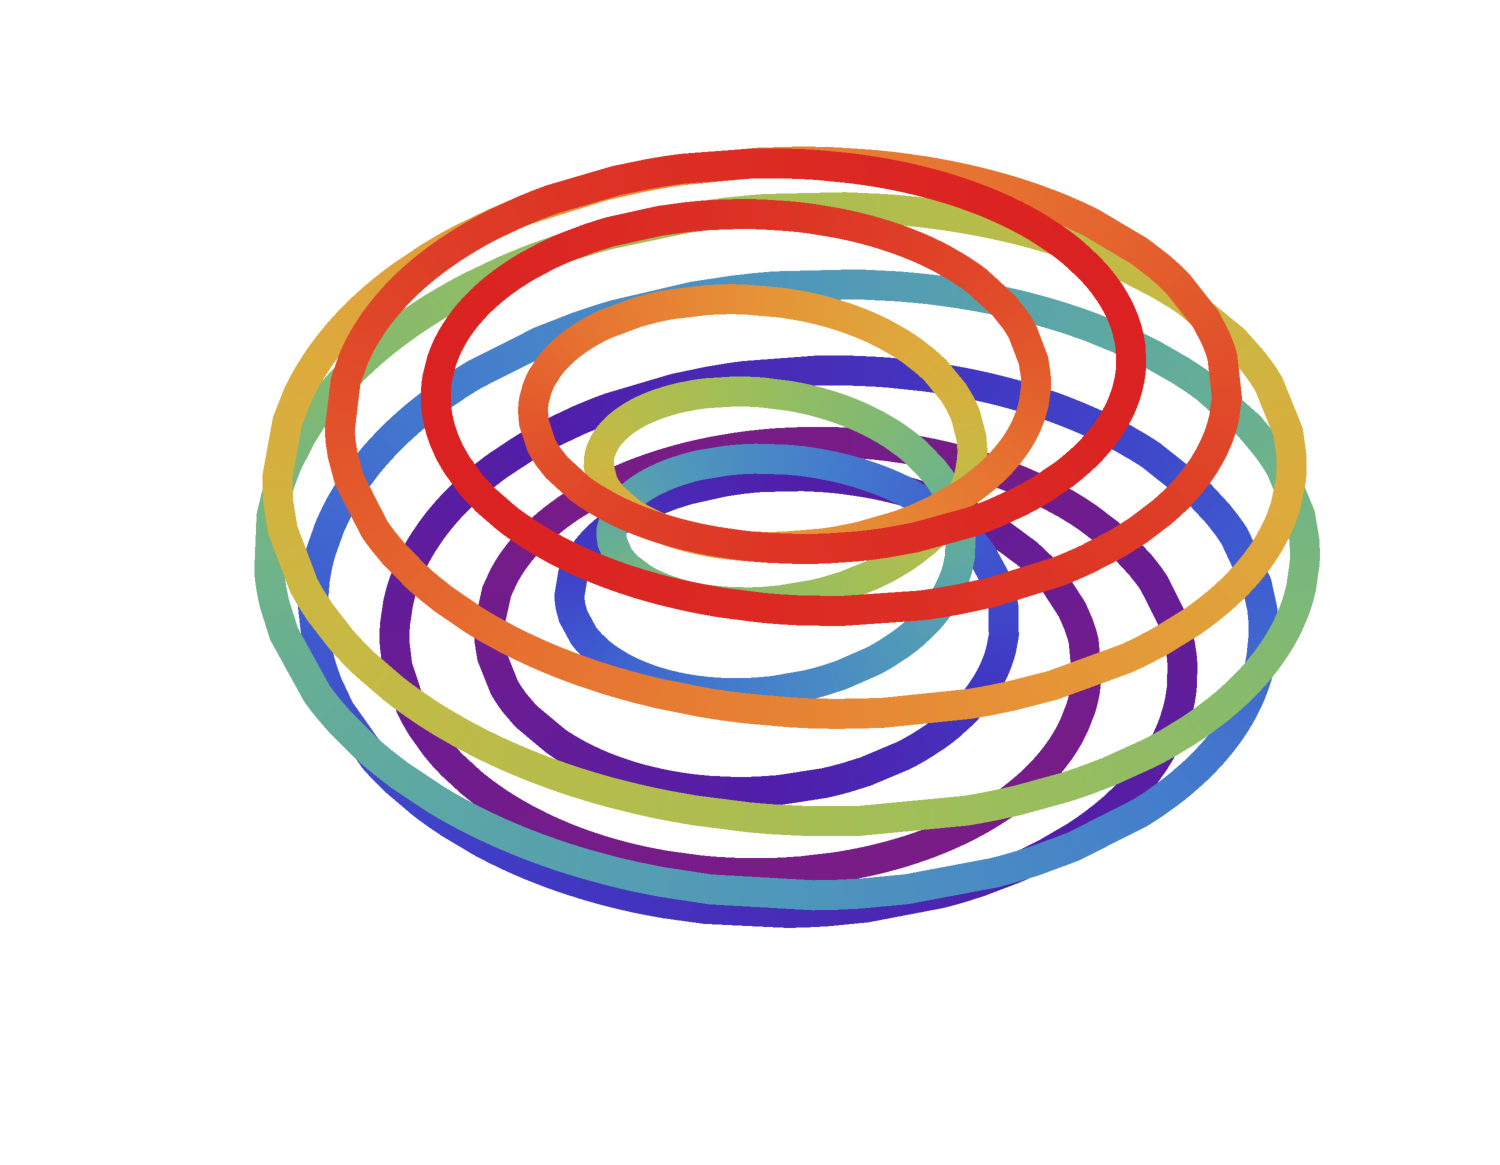
\includegraphics[width=\linewidth]{../data/torus-p11-q2.pdf}
        \subcaption{$p = 11, q = 2$}
    \end{minipage}
\end{figure}

Okazuje się, że innych obiektów już nie ma.

\begin{proposition}
    Jeśli żadna ze składowych splotu torusowego nie jest postaci $K_{0, 0}$ lub $K_{1, 0}$, to splot ten jest równoważny ze splotem $K_{q, r}$ dla pewnych $q, r$.
    Największy wspólny dzielnik indeksów $q, r$ jest jednocześnie liczbą składowych splotu.
\end{proposition}

%Węzeł ten leży na torusie $(r - 2)^2 + z^2 = 1$.
% p = 5;
% q = 3;
% ParametricPlot3D[
% {
% Cos [2 Pi p t] (2 + Cos[2 Pi q t]),
% (2 + Cos[2 Pi q t]) Sin[2 Pi p t],
% -Sin[2 Pi q t]},
% {t, 0, 1},
% ColorFunction -> "Rainbow",
% PlotStyle -> Thickness[0.02],
% Boxed -> False,
% Axes -> False
% ]

Nietrywialne węzły torusowe są pierwsze i odwracalne, ale nie achiralne (mają niezerową sygnaturę).

\begin{proposition}
    Dla $q, r > 0$ zdefiniujmy wielkość $\sigma(q, r) = - \sigma(K_{q, r})$.
    Wtedy, jeśli
    \begin{itemize}[leftmargin=*]
    \itemsep0em
        \item $2r < q$ i $r$ jest parzyste, to $\sigma(q, r) = \sigma(q-2r, r) + r^2$.
        \item $2r < q$ i $r$ jest nieparzyste, to $\sigma(q, r) = \sigma(q-2r, r) + r^2 - 1$.
        \item $\sigma(2r, r) = r^2 - 1$.
        \item jeśli $r \le q < 2r$ i $r$ jest parzyste, to $\sigma(q, r) + \sigma(2r-q, r) = r^2-1$.
        \item jeśli $r \le q < 2r$ i $r$ jest nieparzyste, to $\sigma(q, r) + \sigma(2r-q, r) = r^2-2$.
    \end{itemize}
    Co więcej, $\sigma(q, r) = \sigma(r, q)$, $\sigma(q, 1) = 0$, $\sigma(q, 2) = q-1$.
\end{proposition}

Dowód zawiera praca \cite{litherland81}.

\begin{proposition}
    Ustalmy względnie pierwsze $q, r$ takie, że $|q|, |r| \ge 2$.
    Splot $K(q, r)$ jest równoważny z odwrotnym do niego splotem $K(-q, -r)$.
\end{proposition}

Sploty $K(q, r)$ oraz $K(r, q)$ również są równoważne.
Murasugi prezentuje w książce \cite{murasugi96} przyjemny dowód opierający się na następującym lemacie:
Sfera $S^3$ powstaje z powierzchni dwóch węzłów trywialnych z wnętrzem ($D^2 \times S^1$) przez wzajemne sklejenie południka i równoleżnika z równoleżnikiem i południkiem.

% {\color{red} Longitude, meridian -- ustalić słownictwo}

Macierze Seiferta $M$ mają nieskomplikowaną blokową budowę, która może posłużyć do znalezienia wielomianu Alexandera (wzorem $\Delta = \det (M - tM^t)$).
Rachunki są nieco uciążliwe, oto ich wynik:

\begin{proposition}
    Wielomianem Alexandera splotu torusowego $K(q, r) \neq K(0,0)$ o $d$ składowych jest
    \[
        \Delta_{q, r}(t) = (-1)^{d-1} \frac{(1-t)(1 - t^{qr/d})^d}{(1-t^q)(1-t^r)} \left/t^{(q-1)(r-1)/2}\right. .
    \]
\end{proposition}

Znajomość wielomianu Alexandera wystarcza na szczęście do podania pełnej klasyfikacji węzłów torusowych bez uciążliwego dowodu.

\begin{proposition}
    Węzły torusowe $K(q, r)$, $K(p, s)$ są równoważne wtedy i tylko wtedy, gdy $\{q, r\} = \{p, s\}$ lub $\{q, r\} = \{-p, -s\}$.
\end{proposition}

\begin{proof}
    Ograniczymy się do przypadku, gdy $p, q, r, s \ge 2$.
    Tylko jedna implikacja wymaga dowodu, w prawo.
    Bez straty ogólności załóżmy więc, że $q > r$, $p > s$.
    Skoro węzły $K(q, r)$ i $K(p,s)$ są równoważne, to porównanie najwyższych współczynników w ich wielomianach Alexandera daje równość $(q-1)(r-1) = (p-1)(s-1)$.
    Wymnożenie wszystkiego prowadzi do czterech przypadków: $s = r$, $s = ps$, $qr = r$, $qr = ps$, z których dwa środkowe nie mogą zachodzić (gdyż $p, q > 1$).
    Z czwartego wynika, że $qr \le s < ps$, czyli sprzeczność.
\end{proof}

Podamy teraz wartości całkowitoliczbowych niezmienników dla węzłów torusowych przy założeniu, że $q$ lub $r$ nie jest zerem.

\begin{proposition}[Murasugi, 1991]
    Mamy $cr(K_{q,r}) = \min\{|q|(|r| -1), |r|(|q|-1)\}$.
\end{proposition}

Wyznaczenie indeksu rozwiązującego było dużo trudniejsze.
Murasugi pisze w książce \cite{murasugi96}, że mamy nierówność
\[
    u(K(q, r)) \le \frac 12 (q-1)(r-1),
\]
z równością dla względnie pierwszych $q, r > 0$.
Hipoteza Milnora głosiła, że w rzeczywistości równość zachodzi zawsze.
Dowód został odnaleziony w latach 1993-1995 przy użyciu tzw. \emph{gauge theory} (działu teorii pola, gdzie lagranżjan jest niezmienniczy względem grup Liego lokalnych transformacji...).
Patrz prace \cite{kronheimer93} oraz \cite{kronheimer95}.

\begin{proposition}[Kronheimer, Mrówka] \label{torus_unknotting}
    Dla względnie pierwszych $q, r > 0$ mamy
    \[
        u(K(q, r)) = \frac 12 (q-1)(r-1),
    \]
\end{proposition}

Genus pokrywa się z liczbą gordyjską dla węzłów (czyli względnie pierwszych $q, r$).

\begin{proposition} \label{torus_bridge}
    Indeksem mostowym węzła $K_{q,r}$ jest mniejsza z liczb $|q|, |r|$.
\end{proposition}

\begin{proposition}
    Mamy $\bracket{K_{2, n}} = A \bracket{K_{2,n-1}} + (-1)^{n-1} A^{2-3n}$
    oraz $\bracket{K_{2,1}} = -A^3$.
\end{proposition}

\begin{proposition}
    Wielomianem Jonesa węzła $(m, n)$-torusowego jest
    \[
        V(t) = \frac {t^{(m-1)(n-1):2}}{1-t^2} \cdot (1 - t^{m+1} - t^{n+1} + t^{m+n}).
    \]
\end{proposition}

Murasugi i Neuwirth w 1961 dla węzłów alternujących,
zaś Burde z Zieschangiem w 1965 pokazali, że nietrywialny węzeł,
którego grupa ma nietrywialne centrum, jest torusowy.

\begin{proposition}
    Wielomianem Alexandera węzła $(p,q)$-torusowego jest
    \[
         \Delta(T_{p,q}) = \frac{(t^{pq}-1)(t-1)}{(t^p-1)(t^q-1)}.
    \]
\end{proposition}

\begin{proof}
    Przypadek $p = 2$ wymaga prostego rozumowania indukcyjnego.
    Samo ćwiczenie pojawia się w wielu podręcznikach topologii.
    Pełny dowód można znaleźć w przykładzie 9.15 książki ,,Knots'' Burdego oraz Zieschanga.
    Inne podejście, tak zwaną formułę Seiferta-Torresa, prezentuje przeglądowa praca Turaewa ,,Reidemeister torsion in knot theory'', 119-182.
\end{proof}

\begin{corollary}
    Wielomian Alexandera odróżnia od siebie węzły $(2,n)$-torusowe.
\end{corollary}

\begin{proof}
    Mamy $\Delta(T_{2,n}) = (t^n+1) / (t+1)$, więc $\deg \Delta (T_{2,n}) = n - 1$.
\end{proof}

% Koniec sekcji Węzły torusowe


\section{Węzły satelitarne}

% DIKTJONARY;latitude;szerokość geograficzna;geografia
% DIKTJONARY;longitude;długość geograficzna;geografia
% DIKTJONARY;meridian (of longitude);południk;geografia
% DIKTJONARY;parallel (of latitude);równoleżnik;geografia
% DIKTJONARY;---;geografia;-
% to jest powtórzenie np. z pliku 103a
Załóżmy, że w dopełnieniu pewnego splotu został zanurzony torus.
Jeżeli jest ściśliwy, to albo równoleżnikl torusa ogranicza dysk w dopełnieniu splotu~i torus jest niezawęźlony, albo południk ogranicza dysk w dopełnieniu splotu i~splot nie przebiega wzdłuż torusa.
Żadna z~tych sytuacji nie jest ciekawa.
Inny zdegenerowany przypadek występuje, gdy torus stanowi rurowe otoczenie jednego z~ogniw splotu.
W przeciwnym razie splot można zbudować z~prostszych obiektów.

Oto formalny opis konstrukcji.
Niech $W$ będzie pełnym torusem.
Dysk zanurzony w $W$, którego brzeg stanowi nieściągalną pętlę w $\partial W$, nazywamy południkowym.
Mówimy, że zamknięta krzywa $\lambda \subseteq W$ jest właściwa, jeżeli przecina wszystkie dyski południkowe.

\begin{definition}[węzeł satelitarny]
    \index{węzeł!satelitarny}
    Niech $P$ będzie splotem zanurzonym w~niezawęźlonym torusie $W$ tak, by co najmniej jedno z~ogniw stanowiło właściwą pętlę w~$W$.
    Niech $C$ będzie węzłem, zaś $V$ jego rurowym otoczeniem.
    Wybierzmy dowolny homeomorfizm $h \colon W \to V$.
    Wtedy splot $S = h(P)$ nazywamy satelitą o~wzorcu $P$ oraz towarzyszu $C$.
\end{definition}

% \begin{definition}
%     Węzeł nazywamy satelitarnym, jeśli zawiera nieściśliwy, nierównoległy do brzegu torus we własnym dopełnieniu.
% \end{definition}

Hoste i inni podejrzewają w~\cite{thistlethwaite98}, że jeśli satelita owija się $m$-krotnie wokół torusa, zaś indeks skrzyżowaniowy towarzysza wynosi $k$, to satelita nie posiada diagramu o~mniej niż $km^2$ skrzyżowaniach.
\index[persons]{Hoste, Jim}%
\index[persons]{Thistlethwaite, Morwen}%
\index[persons]{Weeks, Jeff}%

Ponieważ dla trójlistnika $k = 3$, napotkali się tylko na satelity owijające się $m = 2$ razy podczas tablicowania pierwszych węzłów do 16 skrzyżowań.
Nie spodziewano się żadnego satelity ósemki, gdyż wtedy $k = 4$, zatem każdy satelita miałby co najmniej $4 \cdot 2^2 + 1 = 17$ skrzyżowań: dodatkowe $+1$ jest potrzebne, by nie dostać splotu o~dwóch ogniwach.

Najprostszy satelita ma 13 skrzyżowań.
Ze strony internetowej programu Regina można dowiedzieć się dokładniej, jak wygląda rozkład satelitów wśród małych węzłów:

\renewcommand*{\arraystretch}{1.4}
\footnotesize
\begin{longtable}{lccccccc}
    \hline
    \textbf{skrzyżowania} & 13 & 14 & 15 & 16 & 17 & 18 & 19 \\ \hline \endhead
    węzły pierwsze, satelitarne & 2 & 2 & 6 & 10 & 29 & 86 & 245 \\
    \hline
\end{longtable}
\normalsize

Razem 380 węzłów.

\begin{example}[torus połykająco-podążający]
\label{swallow_follow_torus}
% DICTIONARY;swallow-follow;połykająco-podążający;torus
% DICTIONARY;torus;torus;-
    Klasa węzłów satelitarnych obejmuje węzły złożone.
    W ich przypadku można wskazać pewien szczególny torus nieściśliwy -- połykający pierwszy składnik, a~potem podążający za drugim:\footnote{Źródło obrazka: \url{https://mcm-www.jwu.ac.jp/~hayashic/semi/07/07i/07i.html}}
    \begin{figure}[H]
        \centering
        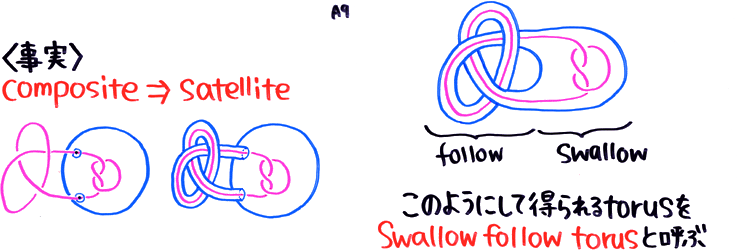
\includegraphics[width=0.75\linewidth]{../data/mixed/follow-swallow.png}
        \caption[something]{Torus połykająco-podążający. Źródło: strona internetowa  C. Hayashiego.}
    \end{figure}
\end{example}

Schubert pokazał, że zorientowane klasy izotopii węzłów w~$S^3$ tworzą wolny przemienny monoid na przeliczalnie wielu generatorach.
\index[persons]{Schubert, Horst}%
Dowód to uważna analiza nieściśliwych torusów obecnych w~dopełnieniu sumy spójnej.
To doprowadziło go do definicji węzłów satelitarnych i~towarzyszących w~przełomowej pracy \cite{schubert53} oraz zunifikowało teorię 3-rozmaitości z teorią węzłów.
Może warto zapoznać się z pracą Motegiego \cite{motegi97}?
Wikipedia mówi, że zapis węzła jako satelity nie jest jednoznaczny, a~tam mogą być przykłady.
%=% https://en.wikipedia.org/wiki/Satellite_knot#cite_ref-7

Na brzegu torusa $V$ można wprowadzić pewien układ współrzędnych: południk to pętla właściwa w $\partial V$, która ogranicza dysk w $V$, natomiast równoleżnik to pętla w $\partial V$, która spotyka południk raz.
Z~dokładnością do izotopii południk jest jeden, ale równoleżnik nie.
Równoleżnik preferowany to taki, którego indeks zaczepienia z~rdzeniem torusa wynosi zero.

\begin{definition}[dubel Whiteheada]
\index{dubel Whiteheada}%
    Jeżeli $P \subseteq W$ jest skręconym jednokrotnie niewęzłem, to węzeł $S$ nazywamy dublem Whiteheada.
\end{definition}

Każdy węzeł posiada nieskończenie wiele dubli Whiteheada: wystarczy rozciąć torus $V$, skręcić jedną końcówkę i~ponownie zszyć, żaden z~nich nie jest odróżniany od niewęzła przez wielomian Alexandera.

Wyróżnia się pewien szczególny homeomorfizm $h$, który przenosi południk i preferowany równoleżnik $W$ na południk i preferowany równoleżnik $V$.
Nazywamy go wiernym.
% DICTIONARY;faithful homeomorphism;homomorfizm wierny;-
O dublu względem wiernego homeomorfizmu mówimy, że jest nieskręcony.
% TODO: skąd powyższe zdanie? jak jest nieskręcony po angielsku?
% Kawauchi około strony 32? (Ten z 1996)

\begin{definition}[węzeł kablowy]
\index{węzeł!kablowy}%
    Niech $h \colon W \to V$ będzie wiernym homeomorfizmem, zaś $P$ węzłem $(p, q)$-torusowym.
    Satelitę $S$ nazywamy węzłem $(p, q)$-kablowym albo krótko kablem.
\end{definition}

\begin{proposition}
    Każdy kabel wyznacza jednoznacznie węzeł, z~którego powstał.
\end{proposition}

\begin{proof}
\index[persons]{Feustel, Charles}%
\index[persons]{Whitten, Wilbur}%
    Wniosek 2 z~pracy \cite{feustel78} Feustela, Whittena pokazuje, że na podstawie kabla można wyznaczyć parametry węzła torusowego $K'_{p,q}$ oraz topologię dopełnienia oryginalnego węzła.
    Wiemy jednak z~twierdzenia Gordona-Lueckego, że różne węzły PIERWSZE mają różne dopełnienia.
\end{proof}

Niewęzeł nie ma nietrywialnych węzłów towarzyszących.

\begin{definition}
    Towarzysza $C$ nietrywialnego splotu nazywamy właściwym, jeśli nie jest niewęzłem i~nie jest ogniwem tego splotu.
\end{definition}

Sploty bez właściwych towarzyszy określa się zazwyczaj terminem ,,atoroidalny''.
\index{splot!atoroidalny}%
Patrz też diagram przedstawiony w \cite{cromwell04} na stronie 83.

Schubert \cite{schubert54} zastanawiał się, czy węzeł może mieć nieskończenie wiele towarzyszy.
Udzielił negatywnej odpowiedzi: satelita $S$ z towarzyszem $C$ oraz wzorcem indeksu $k$ spełnia nierówność $\bridge(S) \ge k \cdot \bridge(C)$; z drugiej strony tylko niewęzeł jest 1-mostowy.
(Patrz też wstęp do \cite{schultens03}).
% wiem to z pracy schultens03

\begin{proposition}
    Duble nietrywialnych węzłów oraz kable są pierwsze.
\end{proposition}

\begin{proof}
    Prosty wniosek z~twierdzenia 4.4.1 w~\cite[s. 84]{cromwell04}: jeżeli wzorzec jest niewęzłem lub węzłem pierwszym, to każdy właściwy satelita jest pierwszy.
\end{proof}

Niektóre węzły przedstawiają się jako satelity w~dokładnie jeden sposób, inne nie.
Rok 1979 przyniósł amerykańską pracę \cite{jaco79} oraz niemiecką książkę\footnote{Według recenzji Hempela, najważniejsze tam jest twierdzenie klasyfikacyjne: niech $M_1, M_2$ będą 3-rozmaitościami Hakena \index{rozmaitość!Hakena} z brzegiem, zaś $V_1, V_2$ ich podrozmaitościami charakterystycznymi, wtedy każda homotopijna równoważność $f \colon M_1 \to M_2$ można zdeformować tak, że jest homeomorfizmem między domknięciami: $M_1 \setminus V_1$ oraz $M_2 \setminus V_2$ i~homotopijną równoważnością między $V_1$ oraz $V_2$.} \cite{johannson79}, gdzie niezależnie od siebie opisano jednoznaczny rozkład (nazywany teraz) Jaco-Shalena-Johannsona:
\index{rozkład Jaco-Shalena-Johannsona}%
\index[persons]{Jaco, William}%
\index[persons]{Shalen, Peter}%
\index[persons]{Johannson, Klaus}%

\begin{proposition}
    Niech $M$ będzie nierozkładalną, orientowalną, domkniętą 3-rozmaitością.
    Istnieje wtedy jedyna z dokładnością do izotopii minimalna rodzina rozłącznie zanurzonych nieściśliwych torusów tak, że każda składowa 3-rozmaitości powstałej przez rozcinanie wzdłuż torusów jest atoroidalna lub włóknistą przestrzenią Seiferta ($S^1$-wiązką nad dwuwymiarowym orbifoldem).
\index{orbifold}%
\index{rozmaitość!atoroidalna}%
\index{przestrzeń!włóknista Seiferta}%
\index{wiązka ($S^1$)}%
\end{proposition}

Jest on związany z operacją złączania (ang. \emph{splicing}), będącej uogólnieniem budowania satelitów, sumy spójnej, dubli Whiteheada i kasowania ogniwa.
\index{złączanie (splicing)}%
% https://arxiv.org/pdf/math/0506523.pdf
% DICTIONARY;splicing;złączanie;-
Hipotezę o jedyności rozkładu wysnuł wcześniej Waldhausen.
\index[persons]{Waldhausen, Friedhelm}%

% Koniec sekcji Węzły satelitarne


\section{Węzły hiperboliczne} % (fold)
\label{sec:hyperbolic}
Jak pisaliśmy w sekcji \ref{mutants_mutation}, słynne węzły Conwaya oraz Kinoshity-Terasakiego odróżnił od siebie po raz pierwszy przez Rileya.
Zbadał paraboliczne reprezentacje ich grup w skończoną grupę prostą $PSL(2, 7)$, co doprowadziło go do odkrycia w dopełnieniu ósemki struktury hiperbolicznej \cite{riley75}.
% https://arxiv.org/pdf/2002.00564.pdf
Zainspirowany tym wynikiem Thurston najpierw rozłożył dopełnienie ósemki na dwa idealne wielościany, a potem znacznie uogólnił swój przykład.

Reszta sekcji powstała na podstawie przeglądowej pracy \cite{purcell19} Futera, Kalfagianniego, Purcell i innych oraz notatek z~wykładów, które były prowadzone przez samą Purcell.
Wiedzę o~węzłach hiperbolicznych można czerpać także z~artykułu: \cite{weeks05} Weeksa.
Poprawiona wersja dostępna w~serwisie arXiv.

% Badając sploty nie ograniczamy się tylko do diagramów, ale korzystamy też z ich dopełnień, to znaczy 3-rozmaitości $S^3 \setminus L$.
% Jest ona homeomorficzna z wnętrzem zwartej rozmaitości $X(L) = S^3 \setminus N(K)$, zwanej zewnętrzem splotu, gdzie $N(L)$ stanowi rurowe otoczenie splotu.
% Dalej możemy stosować maszynierę topologii 3-rozmaitości.

% \begin{definition}[ściśliwy]
%     Niech orientowalna powierzchnia $S$ będzie właściwie\footnote{properly} zanurzona w zwartej, orientowalnej 3-rozmaitości $M$.
%     Załóżmy, że dla każdego dysku $E \subseteq M$ z brzegiem $\partial E \subseteq S$ istnieje dysk $E' \subseteq S$ taki, że $\partial E = \partial E'$.
%     Mówimy wtedy, że powierzchnia $S$ jest nieściśliwa.
% \end{definition}

% $\partial$-ściśliwość

% essential

% Haken

% monodromy of fibration

% Węzły i sploty, które będziemy rozpatrywać dalej, mają szczególną strukturą geometryczną.

\begin{definition}[hiperboliczny]
    \index{węzeł!hiperboliczny}
    Splot $L$, na dopełnieniu którego można zadać zupełną metrykę o stałej krzywiźnie $-1$ nazywamy hiperbolicznym.
\end{definition}

\begin{proposition}
    Splot $L$ jest hiperboliczny wtedy i tylko wtedy, gdy $S^3 \setminus L = \mathbb H^3 / \Gamma$, gdzie $\mathbb H^3$ to hiperboliczna 3-przestrzeń, zaś $\Gamma$ jest dyskretną, beztorsyjną grupą izometrii, izomorficzną z $\pi_1(S^3 \setminus L)$.
\end{proposition}

Thurston podejrzewał, że każda 3-rozmaitość rozkłada się wzdłuż sfer i nieściśliwych torusów na części wyposażone w jedną z ośmiu kanonicznych geometrii:
\begin{itemize}
\item sferyczną $S^3$,
\item euklidesową $E^3$,
\item hiperboliczną $H^3$,
\item $S^2 \times \R$,
\item $H^2 \times \R$,
\item uniwersalne nakrycie $SL(2, \R)$,
\item geometrię Sol albo
\item geometrię Nil.
\end{itemize}
Nie umiał podać pełnego uzasadnienia, w 1982 roku udowodnił swoje przypuszczenie dla rozmaitości Hakena.
Dowód hipotezy geometryzacyjnej dostarczył mniej więcej dwie dekady później Perelman, nie to jest jednak dla nas najważniejsze.

Thurston pokazał też, że dopełnienie węzła jest rozmaitością włóknistą Seiferta, toroidalną albo hiperboliczną.
Innymi słowy, przedstawił trychotomię:
\begin{theorem}
    \index{twierdzenie!Thurstona}
    Każdy węzeł jest satelitarny, torusowy albo hiperboliczny.
\end{theorem}

Węzły hiperboliczne stanowią najliczniejszą i najmniej zrozumianą rodzinę węzłów.

\begin{proof}
    Thurston w \cite{thurston82}.
\end{proof}

Dwa lata później Menasco \cite{menasco84} pokazał, że każdy pierwszy, alternujący splot jest albo 2-warkoczem (a zatem, torusowy) albo hiperboliczny.

\begin{corollary}
    Każdy węzeł hiperboliczny jest pierwszy.
\end{corollary}

Prawie każdy węzeł pierwszy o~mniej niż 17 skrzyżowaniach jest hiperboliczny, na 32 wyjątki składa się 12 węzłów torusowych oraz 20 satelitów trójlistnika.
Te ostatnie mają co najmniej 11 skrzyżowań.
Baza ciągów liczb całkowitych OEIS zawiera informacje na temat liczności poszczególnych typów węzłów.
Analizując ciągi A051764, A051765 oraz A052408 można dojść do wniosku, że wraz ze wzrostem liczby skrzyżowań, stosunek liczby węzłów hiperbolicznych do wszystkich węzłów dąży do $1$:

\begin{figure}[H]
\renewcommand*{\arraystretch}{1.4}
\footnotesize
\begin{longtable}{lcccccccccccccc}
\hline
    \textbf{rodzaj} & 3 & 4 & 5 & 6 & 7 & 8  & 9  & 10  & 11  & 12   & 13   & 14    & 15     \\ \hline \endhead
    torusowe        & 1 & 0 & 1 & 0 & 1 & 1  & 1  & 1   & 1   & 0    & 1    & 1     & 2      \\
    satelitarne     & 0 & 0 & 0 & 0 & 0 & 0  & 0  & 0   & 0   & 0    & 2    & 2     & 6      \\
    hiperboliczne   & 0 & 1 & 1 & 3 & 6 & 20 & 48 & 164 & 551 & 2176 & 9985 & 46969 & 253285 \\
    \hline
\end{longtable}
\normalsize
\end{figure}

W pracy \cite{malyutin16} A. Malyutin pokazał jednak, że to przypuszczenie jest sprzeczne z~wieloma innymi starymi hipotezami teorii węzłów: \ref{malyutin1} -- \ref{malyutin4}.

\begin{conjecture}
    \label{malyutin1}
    Indeks skrzyżowaniowy jest addytywny względem sumy spójnej.
\end{conjecture}

(To jest powtórzenie hipotezy \ref{cnj:crossing_additive}).
Murasugi dowiódł prawdziwości hipotezy dla węzłów alternujących, w~pracy \cite{murasugi87} jest to wniosek z~dowodu hipotezy Taita.
Krótko po tym Lickorish, Thistlethwaite powtórzyli to dla węzłów adekwatnych w \cite{lickorish88}.
Na początku XX wieku Diao \cite{diao04} oraz Gruber \cite{gruber03} niezależnie udowodnili hipotezę \ref{malyutin1} dla pewnej szerokiej klasy węzłów, obejmującej wszystkie węzły torusowe oraz wiele węzłów alternujących oraz pewne inne obiekty, których nie chcemy opisywać.

\begin{conjecture}
    Satelita ma większy (w słabszej wersji: nie mniejszy) indeks skrzyżowaniowy niż jego towarzysze.
\end{conjecture}

Lackenby pokazał w~\cite{lackenby14}, że jeśli $K$ jest satelitą z towarzyszem $L$, to $\operatorname{cr} K \ge 10^{-13} \operatorname{cr} L$.

\begin{conjecture}
    Węzeł złożony ma większy (w słabszej wersji: nie mniejszy) indeks skrzyżowaniowy niż jego faktory.
\end{conjecture}

Mówimy, że węzeł pierwszy $P$ jest $\lambda$-regularny, jeśli $cr K \ge \lambda \cdot cr P$ za każdym razem, gdy węzeł $P$ jest faktorem węzła $K$.
Zatem hipotezę można wysłowić krótko ,,węzły pierwsze są $1$-regularne''.
Na podstawie prac Murasugiego, Kauffmana i~Thistlethwaite'a z~końca lat 80. wiemy, że zachodzi dla węzłów alternujących.
Diao pokazał w \cite[tw. 3.8]{diao04}, że węzły torusowe także są $1$-regularne, natomiast Lackenby przedstawił w~\cite{lackenby09} rozumowanie, dlaczego wszystkie węzły są $1/152$-regularne.
Pisaliśmy o tym w podsekcji \ref{sub:crossing_number}.

\begin{conjecture}
    \label{malyutin4}
    Węzły pierwsze są $2/3$-regularne.
\end{conjecture}

Rozwiązanie zagadki przyniosła praca samego Malyutina \cite{malyutin19} opublikowana latem 2019 roku, przynajmniej dla splotów.
Pokazał w~niej, że jeśli oznaczymy liczbę splotów pierwszych i~nierozszczepialnych o~$n$ lub mniej skrzyżowaniach przez $P_n$, zaś liczbę hiperbolicznych splotów, także o~$n$ lub mniej skrzyżowaniach, przez $H_n$, prawdziwe będzie oszacowanie
\begin{equation}
    \liminf_{n \to \infty} \frac{H_n}{P_n} < 1 - 10^{-13}.
\end{equation}

% Every non-split, prime, alternating link that is not a~torus link is hyperbolic by a~result of William Menasco.

% https://arxiv.org/abs/math/0309466
% https://arxiv.org/abs/math/0311380

Czwarty rozdział książki \cite{purcell2020} zawiera ćwiczenie, by znaleźć dwuparametrową rodzinę zupełnych struktur hiperbolicznych na dziurawym torusie oraz czterokrotnie dziurawej sferze.
Elastyczność tego rodzaju nie występuje w przestrzeniach wyższych wymiarów.
Z twierdzenia o sztywności, w wersji algebraicznej:

\begin{theorem}[Mostow-Prasad]
    \index{twierdzenie!o sztywności}
    Niech $\Gamma_1, \Gamma_2$ będą dyskretnymi podgrupami grupy izometrii $\mathbb H^n$ dla $n \ge 3$ takimi, że ilorazy $\mathbb H^n$ mają skończone objętości.
    Załóżmy też, że istnieje izomorfizm grup $\varphi \colon \Gamma_1 \to \Gamma_2$.
    Wtedy podgrupy $\Gamma_1, \Gamma_2$ są sprzężone.
\end{theorem}

albo geometrycznej:

\begin{theorem}[Mostow-Prasad]
    Niech $M_1, M_2$ będą zupełnymi, hiperbolicznymi rozmaitościami o skończonych objętościach.
    Wtedy każdy izomorfizm grup podstawowych $\varphi \colon \pi_1(M_1) \to \pi_1(M_2)$ realizowany jest jednoznacznie przez izometrię.
\end{theorem}

wynika, że jeśli znaleźliśmy jakąś zupełną strukturę hiperboliczną na dopełnieniu splotu, to innych już nie ma. 
Dzięki temu niezmienniki mające korzenie w geometrii hiperbolicznej mają przyjemne własności.
Patrz także oryginalne prace: Mostowa \cite{mostow73}, Prasada \cite{prasad73}.

\begin{proof}
    Thurston przedstawił szkic rozumowania w sekcji 5.9 swoich notatek, na bazie których powstała później książka \cite{thurston97}.
    Inne szczegółowe rozumowanie można znaleźć w rozdziale C podręcznika \cite{benedetti92}.
\end{proof}

% luźno związane: http://www.deltami.edu.pl/temat/matematyka/topologia/2012/12/27/%William_Thurston_i_hipoteza_geometryzacyjna/

\begin{tobedone}[kryterium Thurstona]
    Niech $L$ będzie splotem z dopełnieniem $X$ i grupą podstawową $\pi = \pi_1(X)$.
    Jeżeli spełnione są następujące warunki:
    \begin{enumerate}
    \item $L$ nie rozszczepia się,
    \item $L$ nie jest niewęzłem,
    \item żadna składowa $L$ nie jest niezakłóconym węzłem satelitarnym (?),
    \item $L$ nie jest węzłem torusowym,
    \end{enumerate}
    to $L$ jest splotem hiperbolicznym.
    Warunki podane wyżej mają swoje odpowiedniki dla przestrzeni $X$ ($X$ nie zawiera właściwej 2-sfery, właściwego dysku, właściwego torusa, właściwego pierścienia) oraz grupy $\pi$ ($\pi$ nie jest wolnym produktem, nie jest cykliczna oraz nie zawiera kopii $\Z^2$).
\end{tobedone}

\begin{proposition}
    Grupa symetrii węzła hiperbolicznego jest skończona: cykliczna lub diedralna.
\end{proposition}

Uwaga -- nie chodzi tutaj ani o grupę węzła, ani grupę kolorującą, ale prawdopodobnie grupę automorfizmów zewnętrznych grupy $\pi_1(S^3 \setminus K)$.

\begin{proof}
    Pierwszy był Riley w artykule \cite{riley75}, można też zapoznać się z późniejszą pracą \cite{kodama92} Kodamy.
\end{proof}

% objętość

Twierdzenie Mostowa-Prasada pozwala nam na wprowadzenie nowych niezmienników splotów hiperbolicznych: wystarczy wziąć dowolny geometryczny niezmiennik dopełnienia węzła.
Najważniejszym z nich wydaje się być objętość.

\begin{definition}[objętość]
    Niech $L$ będzie splotem hiperbolicznym.
    Objętość dopełnienia $L$ względem zupełnej metryki hiperbolicznej nazywamy objętością splotu $L$ i oznaczamy $\volume L$.
\end{definition}

Objętość jest zawsze skończoną liczbą rzeczywistą.
Dla wygody przyjmuje się czasami, że objętość węzłów torusowych oraz satelitarnych wynosi $0$.
Komputerowy program SnapPea napisany przez J. Weeksa pozwala na wyznaczenie objętości dowolnego splotu o rozsądnej ilości skrzyżowań.

\begin{example}
    $\volume 4_1 \approx 2.0298832$.
\end{example}

Patrz też ciąg A091518 w bazie danych OEIS.

\begin{proposition}
    \label{least_volume}
    Żaden węzeł nie ma mniejszej objętości hiperbolicznej od ósemki.
\end{proposition}

\begin{proof}
    Cao, Meyerhoff w \cite{cao01} przeanalizowali pakowania horokul w uniwersalnym nakryciu związanym z rozmaitościami.
    Doszli do wniosku, że nie ma tam dostatecznieo wolnego miejsca, jeżeli ostrze (cusp) nie jest odpowiedniego rozmiaru.
    Trzykrotnie wspierają się przy tym pomocą komputera, by sprawdzić, że określone warunki są spełnione we wszystkich punktach danej przestrzeni parametrów.
\end{proof}

\begin{example}
    $\volume 5_2 \approx 2.82812$.
\end{example}

W encyklopedii Wolfram Mathworld znajduje się informacja, że $5_2$ oraz pewien węzeł o~dwunastu skrzyżowaniach mają tę samą objętość, prawdopodobnie chodzi tu o~$12n_{242}$, który znany jest także jako $(-2, 3, 7)$-precel. 

\begin{example}
    $\volume 6_1 \approx 3.16396$.
\end{example}

\begin{example}
    $\volume 6_2 \approx 4.40083$.
\end{example}

\begin{example}
    $\volume 6_3 \approx 5.69302$.
\end{example}

\begin{example}
    $\volume 7_4 \approx 5.13794$.
\end{example}

\begin{example}
    Niech $K$ będzie jednym z dwóch węzłów w parze Perko.
    Wtedy $\volume K \approx 5.63877$.
\end{example}

Praca \cite{purcell19} wspomina kilka przyjemnych ograniczeń, jakie musi spełniać objętość.
Aby je przytoczyć, musimy najpierw zdefiniować dwie stałe: $v_4$ oraz $v_8$, objętość idealnego czworościanu (odpowiednio: ośmiościanu) foremnego w $\mathbb H^3$.
Mamy
\begin{align}
    v_4 & = 1.0149\ldots \\
    v_8 & = 3.6638\ldots
\end{align}

I tak najpierw Adams pokazał:

\begin{proposition}
    Niech $D$ będzie diagramem hiperbolicznego splotu o $\operatorname{cr} L \ge 5$ skrzyżowaniach.
    Wtedy
    \begin{equation}
        \volume (S^3 \setminus K) \le 4 (\operatorname{cr} D - 4) v_4.
    \end{equation} 
\end{proposition}

A później poprawił wswój wynik:

\begin{proposition}
    Niech $D$ będzie diagramem hiperbolicznego splotu o $\operatorname{cr} L \ge 5$ skrzyżowaniach.
    Wtedy
    \begin{equation}
        \volume (S^3 \setminus K) \le 4 (\operatorname{cr} D - 5) v_8 + 4v_4.
    \end{equation} 
\end{proposition}

Jego metoda polega na podzieleniu dopełnienia splotu na czterościany i ośmiościany oraz policzeniu ich.
To, w połączeniu ze znanymi ograniczeniam na objętość ,,cegiełek'', wystarcza.
Podział na ośmiościany zaproponował Dylan Thurston (nie mylić z Williamem!).

% Wiki

Thurston zauważył, że tylko skończenie wiele hiperbolicznych 3-rozmaitości może mieć tę samą objętość -- wynika to z prac Gromova i Jørgensena.
Następnie Wielenberg przedstawił w~\cite{wielenberg81} przykłady pokazujące, że istnieją dowolnie duże kolizje wśród węzłów hiperbolicznych: pewne podgrupy klasycznej grupy Picarda działają  na półprzestrzeni hiperbolicznej wymiaru 3 i mają przy tym fundamentalne wielościany identyczne jako zbiory, ale znacząco różne w~sposobie, w jaki zidentyfikowano ich ściany.

Na przykład mutacja węzła hiperbolicznego nigdy nie zmienia objętości \cite{ruberman87}, \cite[s. 124]{adams94}.
Praktyka pokazuje jednak, że niezmiennik dobrze wspomaga proces tablicowania węzłów.

\begin{proposition}
    Objętości hiperboliczne 3-rozmaitości tworzą dobrze uporządkowany podzbiór $\R$, typu $\omega^\omega$.
\end{proposition}

\begin{proof}
    Wikipedia twierdzi, że dowód jest gdzieś w \cite{neumann85}, ja tego nie widzę.
\end{proof}

W dowolnej rodzinie węzłów istnieje element o najmniejszej objętości.
Dla orientowalnych, niezwartych hiperbolicznych 3-rozmaitości, klasy obejmującej dopełnienia hiperbolicznych węzłów, najmniejszą objętość posiada dopełnienie ósemki oraz jej bliźniak, otrzymany przez $(5, 1)$-chirurgię jednego z ogniw splotu Whiteheada.
To jest fakt \ref{least_volume}.
Natomiast wśród orientowalnych 3-rozmaitości o dwóch ostrzach najmniejszą objętość, ma $(-2, 3, 8)$-precel oraz splot Whiteheada: Agol pokazał to w \cite{agol10}.
Ich objętość wynosi
\begin{equation}
    v_8 = 4 \sum_{n=0}^\infty \frac{(-1)^n}{(2n+1)^2} = \approx 3.6638623767. % ... 08876060218414059729536443096597497126688537065 ...
\end{equation}
Yoshida \cite{yoshida13} znalazł splot z najmniejszą objętością równą $2v_8$ wśród tych o 4 ogniwach, sploty o 3 ogniwach nie są zbyt dobrze zrozumiane.

% Koniec sekcji Węzły hiperboliczne

\section{Węzły plastrowe} % (fold)
\label{sec:slice}
% Na podstawie podręcznika Murasugiego
Rozpatrzmy węzeł $K$ w~sferze $S^3$ jako brzegu czterowymiarowej kuli $B^4$.
Punkt wewnętrzny $P$ dysku $D$ w~tej kuli nazywamy osobliwym, jeśli nie można wskazać dla niego żadnego otoczenia $U$, homeomorficznego z~$B^4$, takiego że $\partial U \cap D$ jest węzłem trywialnym w~$\partial U$, 3-sferze.
Jeśli $K$ jest brzegiem dysku $D$ pozbawionego punktów osobliwych, to jest on węzłem plastrowym.

W tej sekcji opiszemy pewną czterowymiarową własność węzłów.
Węzły plastrowe na sferze $S^3$ to takie, które są brzegiem ładnie zanurzonego dysku $D$ w~4-kuli.
Co dokładnie znaczy wyrażenie ,,ładnie zanurzony'' zależy od kontekstu: istnieją węzły gładko albo też topologicznie plastrowe.
Precyzuje to pochodząca najwyraźniej od Foxa (1962) definicja:

\begin{definition}
    \index{węzeł!plastrowy}
    Węzeł $K \subseteq S^3$ nazywamy plastrowym, jeśli istnieje płaski dysk $D$ zawarty w~$B^4$ taki, że $K = \partial D = D \cap S^3$.
    Płaski, czyli: dysk $D$ posiada otoczenie $N$ będące kopią zbioru $D \times I^2$, która spotyka sferę $S^3$ dokładnie w~$\partial D \times I^2$.
\end{definition}

Następujące węzły o~mniej niż jedenastu skrzyżowaniach są plastrowe: $6_1$, $8_{20}$, $8_{8}$, $8_{9}$, $9_{27}$, $9_{41}$, $9_{46}$, $10_{22}$, $10_{35}$, $10_{3}$, $10_{42}$, $10_{48}$, $10_{75}$, $10_{87}$, $10_{99}$, $10_{123}$, $10_{129}$, $10_{137}$, $10_{140}$, $10_{153}$, $10_{155}$, $10_{155}$.
Lista ta powstała na podstawie portalu KnotAtlas.

\begin{proposition} \label{slice_square_det}
    Wyznacznik węzła plastrowego jest kwadratem (Rolfsen 1976, strona 224).
\end{proposition}

Węzły plastrowe (slice), skręcone (twist).

\begin{definition} \label{twist_knots}
    \index{węzeł!skręcony}
    Węzeł powstały przez $n$-krotne półskręcanie domkniętej pętli oraz splecienie końców nazywamy węzłem skręconym.
\end{definition}

Węzły skręcone to dokładnie towarzyszące niewęzłowi w~węzłach satelitarnych, tak zwane whiteheadowskie duble niewęzła.
Wszystkie są odwracalne (ale tylko niewęzeł oraz ósemka są amfichiralne) i~mają liczbę gordyjską $1$, ponieważ wystarczy rozwiązać skrzyżowanie, które plotło końce.
Każdy jest $2$-mostowy i~posiada zerową sygnaturę.
Dalsze własności węzłów skręconych zależą od $n$, ilości półskrętów.
Indeks skrzyżowaniowy wynosi $n + 2$.

\begin{proposition}
    Wielomianowymi niezmiennikami węzłów skręconych są:
    \begin{align*}
    (q+1)\jones(q) & = \begin{cases}
        1+q^{-2}+q^{-n}-q^{-n-3} & n \mbox{ nieparzyste} \\
        q^{3}+q-q^{3-n}+q^{-n} & n \mbox{ parzyste}
    \end{cases} \\
    2 \conway (z) & = \begin{cases}
        (n+1) z^{2} + 2 & n \mbox{ nieparzyste} \\
        2 - nz^2 & n \mbox{ parzyste}
    \end{cases}
    \end{align*}
\end{proposition}

%\begin{definition}
    %Węzeł $K$ w~$S^3 = \partial D^4$ jest plastrowy, jeśli ogranicza dysk $\alexander^2$ w~$D^4$, który ma rurowe otoczenie $\alexander^2 \times D^2$, którego przekrojem z~$S^3$ jest rurowe otoczenie $K \times D^2$ dla $K$. \index{Węzeł!plastrowy}
%\end{definition}

Istnieje konkurencyjna definicja węzłów plastrowych.
Dwa sploty $K, L \subseteq S^n$ nazywamy zgodnymi (\emph{concordant}), jeśli istnieje włożenie $f \colon K \times [0,1] \to S^n \times [0,1]$ spełniające dwa warunki: $f(K \times 0) = K \times 0$ oraz $f(K \times 1) = L \times 1$.

\begin{definition} \label{def:slice_knot}
    Węzeł zgodny z~niewęzłem nazywamy plastrowym.
\end{definition}

Zgodność jest relacją równoważności, słabszą od izotopii, ale mocniejszą od homotopii.
W zbiorze jej klas abstrakcji, oznaczanym przez $C^1$, można zadać strukturę grupy abelowej izomorficznej z~$\Z^\infty \oplus (\Z/2)^\infty \oplus (\Z/4)^\infty$.
\index{grupa!zgodności}
Działanie dane jest wzorem $[K] + [L] = [K \shrap L]$; niewęzeł stanowi element neutralny.
Elementem odwrotnym do $[K]$ jest $[-K^*]$.

\begin{proposition}
    Albo wszystkie trzy węzły $K, L, K \shrap L$ są plastrowe, albo co najwyżej jeden z~nich.
\end{proposition}

\index{warunek Foxa-Milnora}
Poniższa własność znana jest w~literaturze jako warunek Foxa-Milnora.

\begin{proposition}
    Wielomian Alexandera węzła plastrowego $K$ jest postaci $f(t) f(1/t)$, gdzie $f(t)$ jest pewnym wielomianem Laurenta nad pierścieniem $\Z$.
\end{proposition}

\begin{theorem}[Casson, Gordon, 1975]
    Niewęzeł oraz węzeł dokerski ($6_1$) są jedynymi skręconymi węzłami plastrowymi.
\end{theorem}

\begin{proof}
    Casson, Gordon: ,,Cobordism of classical knots'', Orsay, 1976.
\end{proof}

\begin{definition}
    \index{węzeł!taśmowy}
    Węzeł $K = f(S^1)$ będący brzegiem singularnego dysku $f \colon D \to S^3$ posiadającego następującą własność: każda przecinająca siebie składowa jest łukiem $A \subseteq f(D^2)$, dla którego $f^{-1}(A)$ składa się z~dwóch łuków w~$D^2$ (jeden z~nich jest wewnętrzny), nazywamy taśmowym.
\end{definition}

Suma spójna dowolnego węzła $K$ oraz jego lustra $mK$ jest taśmowa.
Dowód plastrowatości można znaleźć w~Kawauchi, A Survey of knot theory, strona 155.

\begin{proposition}
    Każdy węzeł taśmowy jest plastrowy.
\end{proposition}

Dawno temu Fox zapytał, czy implikacja odwrotna także jest prawdziwa.

\begin{conjecture}[Fox, 1958]
    Każdy węzeł plastrowy jest taśmowy.
\end{conjecture}

W latach sześćdziesiątych podano kryteria na to, by węzeł nie był węzłem plastrowym (Fox-Milnor 1966, Murasugi 1965).
W szczególności, spośród tych o~co najwyżej siedmiu skrzyżowaniach, tylko $6_1$ jest plastrowy.

% http://citeseerx.ist.psu.edu/viewdoc/download?rep=rep1&type=pdf&doi=10.1.1.212.2610
% http://people.brandeis.edu/~ruberman/drslides/wesleyan.pdf

\begin{proposition}
    Niech $K$ będzie węzłem plastrowym.
    Wtedy $\operatorname{Arf} K = 0$.
\end{proposition}

\begin{proof}
    Z kryterium Foxa-Milnora wynika, że wyznacznik węzła
    \begin{equation}
        \det K = |\alexander(-1)| = f(-1)\cdot f(-1)
    \end{equation}
    to kwadrat.
    Fakt \ref{odd_determinant} mówi nam, iż wyznacznik jest jednocześnie liczbą nieparzystą.
    Wynika stąd przystawanie $\det K \equiv 1 \mod 8$, które w~połączeniu z warunkiem Murasugiego (fakt \ref{arf_murasugi}) daje $\operatorname{Arf} K = 0$.
\end{proof}

\begin{proposition} \label{slice_signature}
    Plastrowe węzły mają zerową sygnaturę.
\end{proposition}

\begin{proof}[Szkic dowodu]
    Ustalmy odwzorowanie $f$, które jest niesingularne, symetryczne i~dwuliniowe, z~przestrzeni $V$ o~wymiarze $2n$ oraz wyznaczoną przez nie formę kwadratową.
    Jeśli znika ona na podprzestrzeni wymiaru $n$, to ma zerową sygnaturę.
    %Praca "Infinite Order Amphicheiral Knots". (Charles Livingston, 2001) -- chyba nie?
    (dowód znaleziony w~podręczniku Lickorisha).
    Patrz też twierdzenie 8.8 z~artykułu \cite{murasugi65}.
\end{proof}

Własności opisane w~faktach \ref{slice_square_det} i~\ref{slice_signature} pozwalają stwierdzić, że 223 spośród 249 węzłów pierwszych o~dziesięciu lub mniej skrzyżowaniach nie jest plastrowych.

Każda macierz Seiferta $V$ (całkowitoliczbowa, kwadratowa, taka że $\det (V - V^t) = 1$), która jest unimodularnie sprzężona: istnieje całkowitoliczbowa macierz $P$ o~wyznaczniku równym $\pm 1$, że
\[
    V = P () P^{-1}
\]
stanowi macierz Seiferta pewnego węzła plastrowego.
Takie węzły nazywamy plastrowymi algebraicznie.
Węzeł $K$ w~$S^3$ jest algebraicznie plastrowy dokładnie wtedy, gdy ogranicza izotropiczną powierzchnię w~kuli $B^4$.
Wytłumaczenie w~podręczniku Kawauchiego.

% Koniec sekcji Węzły plastrowe


\part{Załączniki}
\chapterimage{orange2.jpg} % Chapter heading image
\chapterspaceabove{5.75cm} % Whitespace from the top of the page to the chapter title on chapter pages
\chapterspacebelow{7.25cm} % Amount of vertical whitespace from the top margin to the start of the text on chapter pages

\begin{appendices}
    \renewcommand{\chaptername}{Appendix} % Change the chapter name to Appendix, i.e. "Appendix A: Title", instead of "Chapter A: Title" in the headers
    \chapter{Tablice węzłów pierwszych}
    
\section{Wartości niezmienników}

Ta sekcja zawiera dwie tabele, zacznijmy od opisu drugiej.
Przedstawia ona węzły pierwsze o~co najwyżej dwunastu skrzyżowaniach oraz wartości ich niezmienników (całkowitoliczbowych lub wielomianowych).
Zgodnie z~oznaczeniami przyjętymi w reszcie książki, $\unknotting, \braid, \bridge$ to kolejno liczba gordyjska, warkoczowa i~mostowa.
Zapis $2..3$ mówi, że dokładna wartość nie jest znana i leży w przedziale $[2,3]$.
Jeśli liczba mostowa wynosi dokładnie $2$, zamiast niej podajemy nieskracalny ułamek $p/q$, który koduje węzeł.
Dalej, $\det$ jest wyznacznikiem, $\sigma$ sygnaturą.
Wielomian Conwaya $\conway(z)$ dla oszczędności miejsca podajemy jako ciąg współczynników, na przykład $1-1$ jest skrótem od $1-z^2$.
Ostatnia kolumna mówi, czy węzeł alternuje.

Pierwsza tabela stanowi podsumowanie drugiej: mówi, ile różnych wartości przybiera dany niezmiennik wśród węzłów o~danej liczbie skrzyżowań.
Jak widać, wielomian Conwaya radzi sobie najlepiej, ale nie doskonale.
Dane pochodzą z~portalu KnotInfo \cite{knotinfo22} (założonego w 2004 roku przez Charlesa Livingstona, do którego dołączył wkrótce Jae Choon Cha. W 2019 roku w~rozwoju strony zaczęli brać udział jeszcze Allison Moore oraz Eric Ost), gdzie znaleźć można opisy wszystkich niezmienników z~tabeli oraz wiele więcej danych, gorąco zachęcamy do odwiedzin tej strony internetowej.
\index[persons]{Livingston, Charles}%
\index[persons]{Moore, Allison}%
\index[persons]{Ost, Eric}%

    Tabela pierwsza podsumowuje tabelę drugą:
    
\renewcommand*{\arraystretch}{1.4}
\footnotesize
\begin{longtable}{cccccccccc}
\hline
nazwa & u & $\braid$ & $\bridge$ & $\det$ & $\sigma$ & $\conway$ & symetria & alt. & all \\ \hline
\endhead % all the lines above this will be repeated on every page
3 & 1 & 1 & 1 & 1 & 1 & 1 & 1 & 1 & 1 \\
4 & 1 & 1 & 1 & 1 & 1 & 1 & 1 & 1 & 1 \\
5 & 2 & 2 & 1 & 2 & 2 & 2 & 1 & 1 & 2 \\
6 & 1 & 2 & 1 & 3 & 2 & 3 & 2 & 1 & 3 \\
7 & 3 & 3 & 1 & 7 & 4 & 7 & 1 & 1 & 7 \\
8 & 3 & 3 & 2 & 16 & 5 & 21 & 3 & 2 & 21 \\
9 & 4 & 4 & 2 & 29 & 7 & 48 & 2 & 2 & 49 \\
10 & 5 & 4 & 2 & 56 & 7 & 150 & 4 & 2 & 165 \\
11 & 10 & 5 & 3 & 100 & 9 & 419 & 2 & 2 & 552 \\
12 & 10 & 5 & 3 & 167 & 8 & 1513 & 5 & 2 & 2176 \\
\hline
\end{longtable}
\normalsize


    \newpage
    Tabela druga zawiera wartości niezmienników:
    \section{Wartości niezmienników}
\label{sec:table_of_invariants}
Tabela przedstawia węzły pierwsze o~co najwyżej dziesięciu skrzyżowaniach oraz wartości ich niezmienników (całkowitoliczbowych lub wielomianowych).
Zgodnie z~oznaczeniami przyjętymi w reszcie książki, $\operatorname{u}, \operatorname{b}, \operatorname{br}$ to kolejno liczba gordyjska, warkoczowa i~mostowa.
Zapis $2..3$ mówi, że dokładna wartość nie jest znana i leży w przedziale $[2,3]$.
Jeśli liczba mostowa wynosi dokładnie $2$, zamiast niej podajemy nieskracalny ułamek $p/q$, który koduje węzeł.
Dalej, $\det$ jest wyznacznikiem, $\sigma$ sygnaturą, Arf -- oczywiście niezmiennikiem Arfa.
Wielomian Conwaya $\nabla(z)$ dla oszczędności miejsca podajemy jako ciąg współczynników, na przykład $1-1$ jest skrótem od $1-z^2$.

Dane zawarte w~tej tabeli pochodzą ze strony \url{http://www.indiana.edu/~knotinfo/}.
Jej autorzy, Chuck Livingston z~uniwersytetu Indiany  oraz Jae Choon Cha (z koreańskiego Pohangu) prezentują tam wiele innych niezmienników.

\renewcommand*{\arraystretch}{1.4}
\footnotesize
\begin{longtable}{lccccccllc}
\hline
nazwa & u~& b & br & $\det$ & sygn. & Arf & $\nabla(z)$ & sym. & alt. \\ \hline
\endhead % all the lines above this will be repeated on every page
$3_{1}$     &  $1$     &  $2$  &  $3/1$    &  $3$    &  $-2$  &  $1$  &  $1+1$          &  odwracalny  &  tak  \\
$4_{1}$     &  $1$     &  $3$  &  $5/2$    &  $5$    &  $0$   &  $1$  &  $1-1$          &  całkowicie  &  tak  \\
$5_{1}$     &  $2$     &  $2$  &  $5/1$    &  $5$    &  $-4$  &  $1$  &  $1+3+1$        &  odwracalny  &  tak  \\
$5_{2}$     &  $1$     &  $3$  &  $7/3$    &  $7$    &  $-2$  &  $0$  &  $1+2$          &  odwracalny  &  tak  \\
$6_{1}$     &  $1$     &  $4$  &  $9/7$    &  $9$    &  $0$   &  $0$  &  $1-2$          &  odwracalny  &  tak  \\
$6_{2}$     &  $1$     &  $3$  &  $11/4$   &  $11$   &  $-2$  &  $1$  &  $1-1-1$        &  odwracalny  &  tak  \\
$6_{3}$     &  $1$     &  $3$  &  $13/5$   &  $13$   &  $0$   &  $1$  &  $1+1+1$        &  całkowicie  &  tak  \\
$7_{1}$     &  $3$     &  $2$  &  $7/1$    &  $7$    &  $-6$  &  $0$  &  $1+6+5+1$      &  odwracalny  &  tak  \\
$7_{2}$     &  $1$     &  $4$  &  $11/5$   &  $11$   &  $-2$  &  $1$  &  $1+3$          &  odwracalny  &  tak  \\
$7_{3}$     &  $2$     &  $3$  &  $13/9$   &  $13$   &  $-4$  &  $1$  &  $1+5+2$        &  odwracalny  &  tak  \\
$7_{4}$     &  $2$     &  $4$  &  $15/11$  &  $15$   &  $-2$  &  $0$  &  $1+4$          &  odwracalny  &  tak  \\
$7_{5}$     &  $2$     &  $3$  &  $17/7$   &  $17$   &  $-4$  &  $0$  &  $1+4+2$        &  odwracalny  &  tak  \\
$7_{6}$     &  $1$     &  $4$  &  $19/7$   &  $19$   &  $-2$  &  $1$  &  $1+1-1$        &  odwracalny  &  tak  \\
$7_{7}$     &  $1$     &  $4$  &  $21/8$   &  $21$   &  $0$   &  $1$  &  $1-1+1$        &  odwracalny  &  tak  \\
$8_{1}$     &  $1$     &  $5$  &  $13/11$  &  $13$   &  $0$   &  $1$  &  $1-3$          &  odwracalny  &  tak  \\
$8_{2}$     &  $2$     &  $3$  &  $17/6$   &  $17$   &  $-4$  &  $0$  &  $1+0-3-1$      &  odwracalny  &  tak  \\
$8_{3}$     &  $2$     &  $5$  &  $17/4$   &  $17$   &  $0$   &  $0$  &  $1-4$          &  całkowicie  &  tak  \\
$8_{4}$     &  $2$     &  $4$  &  $19/14$  &  $19$   &  $2$   &  $1$  &  $1-3-2$        &  odwracalny  &  tak  \\
$8_{5}$     &  $2$     &  $3$  &  $3$      &  $21$   &  $-4$  &  $1$  &  $1-1-3-1$      &  odwracalny  &  tak  \\
$8_{6}$     &  $2$     &  $4$  &  $23/10$  &  $23$   &  $-2$  &  $0$  &  $1-2-2$        &  odwracalny  &  tak  \\
$8_{7}$     &  $1$     &  $3$  &  $23/9$   &  $23$   &  $2$   &  $0$  &  $1+2+3+1$      &  odwracalny  &  tak  \\
$8_{8}$     &  $2$     &  $4$  &  $25/9$   &  $25$   &  $0$   &  $0$  &  $1+2+2$        &  odwracalny  &  tak  \\
$8_{9}$     &  $1$     &  $3$  &  $25/7$   &  $25$   &  $0$   &  $0$  &  $1-2-3-1$      &  całkowicie  &  tak  \\
$8_{10}$    &  $2$     &  $3$  &  $3$      &  $27$   &  $2$   &  $1$  &  $1+3+3+1$      &  odwracalny  &  tak  \\
$8_{11}$    &  $1$     &  $4$  &  $27/10$  &  $27$   &  $-2$  &  $1$  &  $1-1-2$        &  odwracalny  &  tak  \\
$8_{12}$    &  $2$     &  $5$  &  $29/12$  &  $29$   &  $0$   &  $1$  &  $1-3+1$        &  całkowicie  &  tak  \\
$8_{13}$    &  $1$     &  $4$  &  $29/11$  &  $29$   &  $0$   &  $1$  &  $1+1+2$        &  odwracalny  &  tak  \\
$8_{14}$    &  $1$     &  $4$  &  $31/12$  &  $31$   &  $-2$  &  $0$  &  $1+0-2$        &  odwracalny  &  tak  \\
$8_{15}$    &  $2$     &  $4$  &  $3$      &  $33$   &  $-4$  &  $0$  &  $1+4+3$        &  odwracalny  &  tak  \\
$8_{16}$    &  $2$     &  $3$  &  $3$      &  $35$   &  $2$   &  $1$  &  $1+1+2+1$      &  odwracalny  &  tak  \\
$8_{17}$    &  $1$     &  $3$  &  $3$      &  $37$   &  $0$   &  $1$  &  $1-1-2-1$      &  ujemny      &  tak  \\
$8_{18}$    &  $2$     &  $3$  &  $3$      &  $45$   &  $0$   &  $1$  &  $1+1-1-1$      &  całkowicie  &  tak  \\
$8_{19}$    &  $3$     &  $3$  &  $3$      &  $3$    &  $-6$  &  $1$  &  $1+5+5+1$      &  odwracalny  &  nie  \\
$8_{20}$    &  $1$     &  $3$  &  $3$      &  $9$    &  $0$   &  $0$  &  $1+2+1$        &  odwracalny  &  nie  \\
$8_{21}$    &  $1$     &  $3$  &  $3$      &  $15$   &  $-2$  &  $0$  &  $1+0-1$        &  odwracalny  &  nie  \\
$9_{1}$     &  $4$     &  $2$  &  $9/1$    &  $9$    &  $-8$  &  $0$  &  $1+10+15+7+1$  &  odwracalny  &  tak  \\
$9_{2}$     &  $1$     &  $5$  &  $15/7$   &  $15$   &  $-2$  &  $0$  &  $1+4$          &  odwracalny  &  tak  \\
$9_{3}$     &  $3$     &  $3$  &  $19/13$  &  $19$   &  $-6$  &  $1$  &  $1+9+9+2$      &  odwracalny  &  tak  \\
$9_{4}$     &  $2$     &  $4$  &  $21/5$   &  $21$   &  $-4$  &  $1$  &  $1+7+3$        &  odwracalny  &  tak  \\
$9_{5}$     &  $2$     &  $5$  &  $23/17$  &  $23$   &  $-2$  &  $0$  &  $1+6$          &  odwracalny  &  tak  \\
$9_{6}$     &  $3$     &  $3$  &  $27/5$   &  $27$   &  $-6$  &  $1$  &  $1+7+8+2$      &  odwracalny  &  tak  \\
$9_{7}$     &  $2$     &  $4$  &  $29/13$  &  $29$   &  $-4$  &  $1$  &  $1+5+3$        &  odwracalny  &  tak  \\
$9_{8}$     &  $2$     &  $5$  &  $31/11$  &  $31$   &  $-2$  &  $0$  &  $1+0-2$        &  odwracalny  &  tak  \\
$9_{9}$     &  $3$     &  $3$  &  $31/9$   &  $31$   &  $-6$  &  $0$  &  $1+8+8+2$      &  odwracalny  &  tak  \\
$9_{10}$    &  $3$     &  $4$  &  $33/23$  &  $33$   &  $-4$  &  $0$  &  $1+8+4$        &  odwracalny  &  tak  \\
$9_{11}$    &  $2$     &  $4$  &  $33/14$  &  $33$   &  $4$   &  $0$  &  $1+4-1-1$      &  odwracalny  &  tak  \\
$9_{12}$    &  $1$     &  $5$  &  $35/13$  &  $35$   &  $-2$  &  $1$  &  $1+1-2$        &  odwracalny  &  tak  \\
$9_{13}$    &  $3$     &  $4$  &  $37/27$  &  $37$   &  $-4$  &  $1$  &  $1+7+4$        &  odwracalny  &  tak  \\
$9_{14}$    &  $1$     &  $5$  &  $37/14$  &  $37$   &  $0$   &  $1$  &  $1-1+2$        &  odwracalny  &  tak  \\
$9_{15}$    &  $2$     &  $5$  &  $39/16$  &  $39$   &  $2$   &  $0$  &  $1+2-2$        &  odwracalny  &  tak  \\
$9_{16}$    &  $3$     &  $3$  &  $3$      &  $39$   &  $-6$  &  $0$  &  $1+6+7+2$      &  odwracalny  &  tak  \\
$9_{17}$    &  $2$     &  $4$  &  $39/14$  &  $39$   &  $-2$  &  $0$  &  $1-2+1+1$      &  odwracalny  &  tak  \\
$9_{18}$    &  $2$     &  $4$  &  $41/17$  &  $41$   &  $-4$  &  $0$  &  $1+6+4$        &  odwracalny  &  tak  \\
$9_{19}$    &  $1$     &  $5$  &  $41/16$  &  $41$   &  $0$   &  $0$  &  $1-2+2$        &  odwracalny  &  tak  \\
$9_{20}$    &  $2$     &  $4$  &  $41/15$  &  $41$   &  $-4$  &  $0$  &  $1+2-1-1$      &  odwracalny  &  tak  \\
$9_{21}$    &  $1$     &  $5$  &  $43/18$  &  $43$   &  $2$   &  $1$  &  $1+3-2$        &  odwracalny  &  tak  \\
$9_{22}$    &  $1$     &  $4$  &  $3$      &  $43$   &  $-2$  &  $1$  &  $1-1+1+1$      &  odwracalny  &  tak  \\
$9_{23}$    &  $2$     &  $4$  &  $45/19$  &  $45$   &  $-4$  &  $1$  &  $1+5+4$        &  odwracalny  &  tak  \\
$9_{24}$    &  $1$     &  $4$  &  $3$      &  $45$   &  $0$   &  $1$  &  $1+1-1-1$      &  odwracalny  &  tak  \\
$9_{25}$    &  $2$     &  $5$  &  $3$      &  $47$   &  $-2$  &  $0$  &  $1+0-3$        &  odwracalny  &  tak  \\
$9_{26}$    &  $1$     &  $4$  &  $47/18$  &  $47$   &  $2$   &  $0$  &  $1+0+1+1$      &  odwracalny  &  tak  \\
$9_{27}$    &  $1$     &  $4$  &  $49/19$  &  $49$   &  $0$   &  $0$  &  $1+0-1-1$      &  odwracalny  &  tak  \\
$9_{28}$    &  $1$     &  $4$  &  $3$      &  $51$   &  $-2$  &  $1$  &  $1+1+1+1$      &  odwracalny  &  tak  \\
$9_{29}$    &  $2$     &  $4$  &  $3$      &  $51$   &  $2$   &  $1$  &  $1+1+1+1$      &  odwracalny  &  tak  \\
$9_{30}$    &  $1$     &  $4$  &  $3$      &  $53$   &  $0$   &  $1$  &  $1-1-1-1$      &  odwracalny  &  tak  \\
$9_{31}$    &  $2$     &  $4$  &  $55/21$  &  $55$   &  $-2$  &  $0$  &  $1+2+1+1$      &  odwracalny  &  tak  \\
$9_{32}$    &  $2$     &  $4$  &  $3$      &  $59$   &  $2$   &  $1$  &  $1-1+0+1$      &  chiralny    &  tak  \\
$9_{33}$    &  $1$     &  $4$  &  $3$      &  $61$   &  $0$   &  $1$  &  $1+1+0-1$      &  chiralny    &  tak  \\
$9_{34}$    &  $1$     &  $4$  &  $3$      &  $69$   &  $0$   &  $1$  &  $1-1+0-1$      &  odwracalny  &  tak  \\
$9_{35}$    &  $3$     &  $5$  &  $3$      &  $27$   &  $-2$  &  $1$  &  $1+7$          &  odwracalny  &  tak  \\
$9_{36}$    &  $2$     &  $4$  &  $3$      &  $37$   &  $4$   &  $1$  &  $1+3-1-1$      &  odwracalny  &  tak  \\
$9_{37}$    &  $2$     &  $5$  &  $3$      &  $45$   &  $0$   &  $1$  &  $1-3+2$        &  odwracalny  &  tak  \\
$9_{38}$    &  $3$     &  $4$  &  $3$      &  $57$   &  $-4$  &  $0$  &  $1+6+5$        &  odwracalny  &  tak  \\
$9_{39}$    &  $1$     &  $5$  &  $3$      &  $55$   &  $2$   &  $0$  &  $1+2-3$        &  odwracalny  &  tak  \\
$9_{40}$    &  $2$     &  $4$  &  $3$      &  $75$   &  $-2$  &  $1$  &  $1-1-1+1$      &  odwracalny  &  tak  \\
$9_{41}$    &  $2$     &  $5$  &  $3$      &  $49$   &  $0$   &  $0$  &  $1+0+3$        &  odwracalny  &  tak  \\
$9_{42}$    &  $1$     &  $4$  &  $3$      &  $7$    &  $2$   &  $0$  &  $1-2-1$        &  odwracalny  &  nie  \\
$9_{43}$    &  $2$     &  $4$  &  $3$      &  $13$   &  $-4$  &  $1$  &  $1+1-3-1$      &  odwracalny  &  nie  \\
$9_{44}$    &  $1$     &  $4$  &  $3$      &  $17$   &  $0$   &  $0$  &  $1+0+1$        &  odwracalny  &  nie  \\
$9_{45}$    &  $1$     &  $4$  &  $3$      &  $23$   &  $2$   &  $0$  &  $1+2-1$        &  odwracalny  &  nie  \\
$9_{46}$    &  $2$     &  $4$  &  $3$      &  $9$    &  $0$   &  $0$  &  $1-2$          &  odwracalny  &  nie  \\
$9_{47}$    &  $2$     &  $4$  &  $3$      &  $27$   &  $-2$  &  $1$  &  $1-1+2+1$      &  odwracalny  &  nie  \\
$9_{48}$    &  $2$     &  $4$  &  $3$      &  $27$   &  $2$   &  $1$  &  $1+3-1$        &  odwracalny  &  nie  \\
$9_{49}$    &  $3$     &  $4$  &  $3$      &  $25$   &  $-4$  &  $0$  &  $1+6+3$        &  odwracalny  &  nie  \\
$10_{1}$    &  $1$     &  $6$  &  $17/15$  &  $17$   &  $0$   &  $0$  &  $1-4$          &  odwracalny  &  tak  \\
$10_{2}$    &  $3$     &  $3$  &  $23/8$   &  $23$   &  $-6$  &  $0$  &  $1+2-5-5-1$    &  odwracalny  &  tak  \\
$10_{3}$    &  $2$     &  $6$  &  $25/6$   &  $25$   &  $0$   &  $0$  &  $1-6$          &  odwracalny  &  tak  \\
$10_{4}$    &  $2$     &  $5$  &  $27/20$  &  $27$   &  $2$   &  $1$  &  $1-5-3$        &  odwracalny  &  tak  \\
$10_{5}$    &  $2$     &  $3$  &  $33/13$  &  $33$   &  $4$   &  $0$  &  $1+4+7+5+1$    &  odwracalny  &  tak  \\
$10_{6}$    &  $3$     &  $4$  &  $37/16$  &  $37$   &  $-4$  &  $1$  &  $1-1-6-2$      &  odwracalny  &  tak  \\
$10_{7}$    &  $1$     &  $5$  &  $43/16$  &  $43$   &  $-2$  &  $1$  &  $1-1-3$        &  odwracalny  &  tak  \\
$10_{8}$    &  $2$     &  $4$  &  $29/6$   &  $29$   &  $-4$  &  $1$  &  $1-3-7-2$      &  odwracalny  &  tak  \\
$10_{9}$    &  $1$     &  $3$  &  $39/28$  &  $39$   &  $-2$  &  $0$  &  $1-2-7-5-1$    &  odwracalny  &  tak  \\
$10_{10}$   &  $1$     &  $5$  &  $45/17$  &  $45$   &  $0$   &  $1$  &  $1+1+3$        &  odwracalny  &  tak  \\
$10_{11}$   &  $2..3$  &  $5$  &  $43/13$  &  $43$   &  $-2$  &  $1$  &  $1-5-4$        &  odwracalny  &  tak  \\
$10_{12}$   &  $2$     &  $4$  &  $47/17$  &  $47$   &  $2$   &  $0$  &  $1+4+6+2$      &  odwracalny  &  tak  \\
$10_{13}$   &  $2$     &  $6$  &  $53/22$  &  $53$   &  $0$   &  $1$  &  $1-5+2$        &  odwracalny  &  tak  \\
$10_{14}$   &  $2$     &  $4$  &  $57/22$  &  $57$   &  $-4$  &  $0$  &  $1+2-4-2$      &  odwracalny  &  tak  \\
$10_{15}$   &  $2$     &  $4$  &  $43/19$  &  $43$   &  $2$   &  $1$  &  $1+3+6+2$      &  odwracalny  &  tak  \\
$10_{16}$   &  $2$     &  $5$  &  $47/33$  &  $47$   &  $-2$  &  $0$  &  $1-4-4$        &  odwracalny  &  tak  \\
$10_{17}$   &  $1$     &  $3$  &  $41/9$   &  $41$   &  $0$   &  $0$  &  $1+2+7+5+1$    &  całkowicie  &  tak  \\
$10_{18}$   &  $1$     &  $5$  &  $55/23$  &  $55$   &  $-2$  &  $0$  &  $1-2-4$        &  odwracalny  &  tak  \\
$10_{19}$   &  $2$     &  $4$  &  $51/14$  &  $51$   &  $-2$  &  $1$  &  $1+1+5+2$      &  odwracalny  &  tak  \\
$10_{20}$   &  $2$     &  $5$  &  $35/16$  &  $35$   &  $-2$  &  $1$  &  $1-3-3$        &  odwracalny  &  tak  \\
$10_{21}$   &  $2$     &  $4$  &  $45/16$  &  $45$   &  $-4$  &  $1$  &  $1+1-5-2$      &  odwracalny  &  tak  \\
$10_{22}$   &  $2$     &  $4$  &  $49/36$  &  $49$   &  $0$   &  $0$  &  $1-4-6-2$      &  odwracalny  &  tak  \\
$10_{23}$   &  $1$     &  $4$  &  $59/23$  &  $59$   &  $2$   &  $1$  &  $1+3+5+2$      &  odwracalny  &  tak  \\
$10_{24}$   &  $2$     &  $5$  &  $55/24$  &  $55$   &  $-2$  &  $0$  &  $1-2-4$        &  odwracalny  &  tak  \\
$10_{25}$   &  $2$     &  $4$  &  $65/24$  &  $65$   &  $-4$  &  $0$  &  $1+0-4-2$      &  odwracalny  &  tak  \\
$10_{26}$   &  $1$     &  $4$  &  $61/44$  &  $61$   &  $0$   &  $1$  &  $1-3-5-2$      &  odwracalny  &  tak  \\
$10_{27}$   &  $1$     &  $4$  &  $71/27$  &  $71$   &  $2$   &  $0$  &  $1+2+4+2$      &  odwracalny  &  tak  \\
$10_{28}$   &  $2$     &  $5$  &  $53/19$  &  $53$   &  $0$   &  $1$  &  $1+3+4$        &  odwracalny  &  tak  \\
$10_{29}$   &  $2$     &  $5$  &  $63/26$  &  $63$   &  $-2$  &  $0$  &  $1-4-1+1$      &  odwracalny  &  tak  \\
$10_{30}$   &  $1$     &  $5$  &  $67/26$  &  $67$   &  $-2$  &  $1$  &  $1+1-4$        &  odwracalny  &  tak  \\
$10_{31}$   &  $1$     &  $5$  &  $57/25$  &  $57$   &  $0$   &  $0$  &  $1+2+4$        &  odwracalny  &  tak  \\
$10_{32}$   &  $1$     &  $4$  &  $69/29$  &  $69$   &  $0$   &  $1$  &  $1-1-4-2$      &  odwracalny  &  tak  \\
$10_{33}$   &  $1$     &  $5$  &  $65/18$  &  $65$   &  $0$   &  $0$  &  $1+0+4$        &  całkowicie  &  tak  \\
$10_{34}$   &  $2$     &  $5$  &  $37/13$  &  $37$   &  $0$   &  $1$  &  $1+3+3$        &  odwracalny  &  tak  \\
$10_{35}$   &  $2$     &  $6$  &  $49/20$  &  $49$   &  $0$   &  $0$  &  $1-4+2$        &  odwracalny  &  tak  \\
$10_{36}$   &  $2$     &  $5$  &  $51/20$  &  $51$   &  $-2$  &  $1$  &  $1+1-3$        &  odwracalny  &  tak  \\
$10_{37}$   &  $2$     &  $5$  &  $53/23$  &  $53$   &  $0$   &  $1$  &  $1+3+4$        &  całkowicie  &  tak  \\
$10_{38}$   &  $2$     &  $5$  &  $59/25$  &  $59$   &  $-2$  &  $1$  &  $1-1-4$        &  odwracalny  &  tak  \\
$10_{39}$   &  $2$     &  $4$  &  $61/22$  &  $61$   &  $-4$  &  $1$  &  $1+1-4-2$      &  odwracalny  &  tak  \\
$10_{40}$   &  $2$     &  $4$  &  $75/29$  &  $75$   &  $2$   &  $1$  &  $1+3+4+2$      &  odwracalny  &  tak  \\
$10_{41}$   &  $2$     &  $5$  &  $71/26$  &  $71$   &  $-2$  &  $0$  &  $1-2-1+1$      &  odwracalny  &  tak  \\
$10_{42}$   &  $1$     &  $5$  &  $81/31$  &  $81$   &  $0$   &  $0$  &  $1+0+1-1$      &  odwracalny  &  tak  \\
$10_{43}$   &  $2$     &  $5$  &  $73/27$  &  $73$   &  $0$   &  $0$  &  $1+2+1-1$      &  całkowicie  &  tak  \\
$10_{44}$   &  $1$     &  $5$  &  $79/30$  &  $79$   &  $-2$  &  $0$  &  $1+0-1+1$      &  odwracalny  &  tak  \\
$10_{45}$   &  $2$     &  $5$  &  $89/34$  &  $89$   &  $0$   &  $0$  &  $1-2+1-1$      &  całkowicie  &  tak  \\
$10_{46}$   &  $3$     &  $3$  &  $3$      &  $31$   &  $-6$  &  $0$  &  $1+0-6-5-1$    &  odwracalny  &  tak  \\
$10_{47}$   &  $2..3$  &  $3$  &  $3$      &  $41$   &  $4$   &  $0$  &  $1+6+8+5+1$    &  odwracalny  &  tak  \\
$10_{48}$   &  $2$     &  $3$  &  $3$      &  $49$   &  $0$   &  $0$  &  $1+4+8+5+1$    &  odwracalny  &  tak  \\
$10_{49}$   &  $3$     &  $4$  &  $3$      &  $59$   &  $-6$  &  $1$  &  $1+7+10+3$     &  odwracalny  &  tak  \\
$10_{50}$   &  $2$     &  $4$  &  $3$      &  $53$   &  $-4$  &  $1$  &  $1-1-5-2$      &  odwracalny  &  tak  \\
$10_{51}$   &  $2..3$  &  $4$  &  $3$      &  $67$   &  $2$   &  $1$  &  $1+5+5+2$      &  odwracalny  &  tak  \\
$10_{52}$   &  $2$     &  $4$  &  $3$      &  $59$   &  $-2$  &  $1$  &  $1+3+5+2$      &  odwracalny  &  tak  \\
$10_{53}$   &  $3$     &  $5$  &  $3$      &  $73$   &  $-4$  &  $0$  &  $1+6+6$        &  odwracalny  &  tak  \\
$10_{54}$   &  $2..3$  &  $4$  &  $3$      &  $47$   &  $2$   &  $0$  &  $1+4+6+2$      &  odwracalny  &  tak  \\
$10_{55}$   &  $2$     &  $5$  &  $3$      &  $61$   &  $-4$  &  $1$  &  $1+5+5$        &  odwracalny  &  tak  \\
$10_{56}$   &  $2$     &  $4$  &  $3$      &  $65$   &  $-4$  &  $0$  &  $1+0-4-2$      &  odwracalny  &  tak  \\
$10_{57}$   &  $2$     &  $4$  &  $3$      &  $79$   &  $2$   &  $0$  &  $1+4+4+2$      &  odwracalny  &  tak  \\
$10_{58}$   &  $2$     &  $6$  &  $3$      &  $65$   &  $0$   &  $0$  &  $1-4+3$        &  odwracalny  &  tak  \\
$10_{59}$   &  $1$     &  $5$  &  $3$      &  $75$   &  $-2$  &  $1$  &  $1-1-1+1$      &  odwracalny  &  tak  \\
$10_{60}$   &  $1$     &  $5$  &  $3$      &  $85$   &  $0$   &  $1$  &  $1-1+1-1$      &  odwracalny  &  tak  \\
$10_{61}$   &  $2..3$  &  $4$  &  $3$      &  $33$   &  $-4$  &  $0$  &  $1-4-7-2$      &  odwracalny  &  tak  \\
$10_{62}$   &  $2$     &  $3$  &  $3$      &  $45$   &  $4$   &  $1$  &  $1+5+8+5+1$    &  odwracalny  &  tak  \\
$10_{63}$   &  $2$     &  $5$  &  $3$      &  $57$   &  $-4$  &  $0$  &  $1+6+5$        &  odwracalny  &  tak  \\
$10_{64}$   &  $2$     &  $3$  &  $3$      &  $51$   &  $-2$  &  $1$  &  $1-3-8-5-1$    &  odwracalny  &  tak  \\
$10_{65}$   &  $2$     &  $4$  &  $3$      &  $63$   &  $2$   &  $0$  &  $1+4+5+2$      &  odwracalny  &  tak  \\
$10_{66}$   &  $3$     &  $4$  &  $3$      &  $75$   &  $-6$  &  $1$  &  $1+7+9+3$      &  odwracalny  &  tak  \\
$10_{67}$   &  $2$     &  $5$  &  $3$      &  $63$   &  $-2$  &  $0$  &  $1+0-4$        &  chiralny    &  tak  \\
$10_{68}$   &  $2$     &  $5$  &  $3$      &  $57$   &  $0$   &  $0$  &  $1+2+4$        &  odwracalny  &  tak  \\
$10_{69}$   &  $2$     &  $5$  &  $3$      &  $87$   &  $2$   &  $0$  &  $1+2-1+1$      &  odwracalny  &  tak  \\
$10_{70}$   &  $2$     &  $5$  &  $3$      &  $67$   &  $2$   &  $1$  &  $1-3-1+1$      &  odwracalny  &  tak  \\
$10_{71}$   &  $1$     &  $5$  &  $3$      &  $77$   &  $0$   &  $1$  &  $1+1+1-1$      &  odwracalny  &  tak  \\
$10_{72}$   &  $2$     &  $4$  &  $3$      &  $73$   &  $-4$  &  $0$  &  $1+2-3-2$      &  odwracalny  &  tak  \\
$10_{73}$   &  $1$     &  $5$  &  $3$      &  $83$   &  $2$   &  $1$  &  $1+1-1+1$      &  odwracalny  &  tak  \\
$10_{74}$   &  $2$     &  $5$  &  $3$      &  $63$   &  $-2$  &  $0$  &  $1+0-4$        &  odwracalny  &  tak  \\
$10_{75}$   &  $2$     &  $5$  &  $3$      &  $81$   &  $0$   &  $0$  &  $1+0+1-1$      &  odwracalny  &  tak  \\
$10_{76}$   &  $2..3$  &  $4$  &  $3$      &  $57$   &  $-4$  &  $0$  &  $1-2-5-2$      &  odwracalny  &  tak  \\
$10_{77}$   &  $2..3$  &  $4$  &  $3$      &  $63$   &  $2$   &  $0$  &  $1+4+5+2$      &  odwracalny  &  tak  \\
$10_{78}$   &  $2$     &  $5$  &  $3$      &  $69$   &  $-4$  &  $1$  &  $1+3+1-1$      &  odwracalny  &  tak  \\
$10_{79}$   &  $2..3$  &  $3$  &  $3$      &  $61$   &  $0$   &  $1$  &  $1+5+9+5+1$    &  ujemny      &  tak  \\
$10_{80}$   &  $3$     &  $4$  &  $3$      &  $71$   &  $-6$  &  $0$  &  $1+6+9+3$      &  chiralny    &  tak  \\
$10_{81}$   &  $2$     &  $5$  &  $3$      &  $85$   &  $0$   &  $1$  &  $1+3+2-1$      &  ujemny      &  tak  \\
$10_{82}$   &  $1$     &  $3$  &  $3$      &  $63$   &  $-2$  &  $0$  &  $1+0-4-4-1$    &  chiralny    &  tak  \\
$10_{83}$   &  $2$     &  $4$  &  $3$      &  $83$   &  $2$   &  $1$  &  $1+1+3+2$      &  chiralny    &  tak  \\
$10_{84}$   &  $1$     &  $4$  &  $3$      &  $87$   &  $-2$  &  $0$  &  $1+2+3+2$      &  chiralny    &  tak  \\
$10_{85}$   &  $2$     &  $3$  &  $3$      &  $57$   &  $4$   &  $0$  &  $1+2+4+4+1$    &  chiralny    &  tak  \\
$10_{86}$   &  $2$     &  $4$  &  $3$      &  $85$   &  $0$   &  $1$  &  $1-1-3-2$      &  chiralny    &  tak  \\
$10_{87}$   &  $2$     &  $4$  &  $3$      &  $81$   &  $0$   &  $0$  &  $1+0-3-2$      &  chiralny    &  tak  \\
$10_{88}$   &  $1$     &  $5$  &  $3$      &  $101$  &  $0$   &  $1$  &  $1-1+2-1$      &  ujemny      &  tak  \\
$10_{89}$   &  $2$     &  $5$  &  $3$      &  $99$   &  $2$   &  $1$  &  $1+1-2+1$      &  odwracalny  &  tak  \\
$10_{90}$   &  $2$     &  $4$  &  $3$      &  $77$   &  $0$   &  $1$  &  $1-3-4-2$      &  chiralny    &  tak  \\
$10_{91}$   &  $1$     &  $3$  &  $3$      &  $73$   &  $0$   &  $0$  &  $1+2+5+4+1$    &  chiralny    &  tak  \\
$10_{92}$   &  $2$     &  $4$  &  $3$      &  $89$   &  $-4$  &  $0$  &  $1+2-2-2$      &  chiralny    &  tak  \\
$10_{93}$   &  $2$     &  $4$  &  $3$      &  $67$   &  $2$   &  $1$  &  $1+1+4+2$      &  chiralny    &  tak  \\
$10_{94}$   &  $2$     &  $3$  &  $3$      &  $71$   &  $-2$  &  $0$  &  $1-2-5-4-1$    &  chiralny    &  tak  \\
$10_{95}$   &  $1$     &  $4$  &  $3$      &  $91$   &  $2$   &  $1$  &  $1+3+3+2$      &  chiralny    &  tak  \\
$10_{96}$   &  $2$     &  $5$  &  $3$      &  $93$   &  $0$   &  $1$  &  $1-3+1-1$      &  odwracalny  &  tak  \\
$10_{97}$   &  $2$     &  $5$  &  $3$      &  $87$   &  $-2$  &  $0$  &  $1+2-5$        &  odwracalny  &  tak  \\
$10_{98}$   &  $2$     &  $4$  &  $3$      &  $81$   &  $-4$  &  $0$  &  $1+0-3-2$      &  chiralny    &  tak  \\
$10_{99}$   &  $2$     &  $3$  &  $3$      &  $81$   &  $0$   &  $0$  &  $1+4+6+4+1$    &  całkowicie  &  tak  \\
$10_{100}$  &  $2..3$  &  $3$  &  $3$      &  $65$   &  $4$   &  $0$  &  $1+4+5+4+1$    &  odwracalny  &  tak  \\
$10_{101}$  &  $3$     &  $5$  &  $3$      &  $85$   &  $-4$  &  $1$  &  $1+7+7$        &  odwracalny  &  tak  \\
$10_{102}$  &  $1$     &  $4$  &  $3$      &  $73$   &  $0$   &  $0$  &  $1-2-4-2$      &  chiralny    &  tak  \\
$10_{103}$  &  $3$     &  $4$  &  $3$      &  $75$   &  $2$   &  $1$  &  $1+3+4+2$      &  odwracalny  &  tak  \\
$10_{104}$  &  $1$     &  $3$  &  $3$      &  $77$   &  $0$   &  $1$  &  $1+1+5+4+1$    &  odwracalny  &  tak  \\
$10_{105}$  &  $2$     &  $5$  &  $3$      &  $91$   &  $-2$  &  $1$  &  $1-1-2+1$      &  odwracalny  &  tak  \\
$10_{106}$  &  $2$     &  $3$  &  $3$      &  $75$   &  $-2$  &  $1$  &  $1-1-5-4-1$    &  chiralny    &  tak  \\
$10_{107}$  &  $1$     &  $5$  &  $3$      &  $93$   &  $0$   &  $1$  &  $1+1+2-1$      &  chiralny    &  tak  \\
$10_{108}$  &  $2$     &  $4$  &  $3$      &  $63$   &  $-2$  &  $0$  &  $1+0+4+2$      &  odwracalny  &  tak  \\
$10_{109}$  &  $2$     &  $3$  &  $3$      &  $85$   &  $0$   &  $1$  &  $1+3+6+4+1$    &  ujemny      &  tak  \\
$10_{110}$  &  $2$     &  $5$  &  $3$      &  $83$   &  $-2$  &  $1$  &  $1-3-2+1$      &  chiralny    &  tak  \\
$10_{111}$  &  $2$     &  $4$  &  $3$      &  $77$   &  $-4$  &  $1$  &  $1+1-3-2$      &  odwracalny  &  tak  \\
$10_{112}$  &  $2$     &  $3$  &  $3$      &  $87$   &  $2$   &  $0$  &  $1+2-1-3-1$    &  odwracalny  &  tak  \\
$10_{113}$  &  $1$     &  $4$  &  $3$      &  $111$  &  $-2$  &  $0$  &  $1+0+1+2$      &  odwracalny  &  tak  \\
$10_{114}$  &  $1$     &  $4$  &  $3$      &  $93$   &  $0$   &  $1$  &  $1+1-2-2$      &  odwracalny  &  tak  \\
$10_{115}$  &  $2$     &  $5$  &  $3$      &  $109$  &  $0$   &  $1$  &  $1+1+3-1$      &  ujemny      &  tak  \\
$10_{116}$  &  $2$     &  $3$  &  $3$      &  $95$   &  $2$   &  $0$  &  $1+0-2-3-1$    &  odwracalny  &  tak  \\
$10_{117}$  &  $2$     &  $4$  &  $3$      &  $103$  &  $2$   &  $0$  &  $1+2+2+2$      &  chiralny    &  tak  \\
$10_{118}$  &  $1$     &  $3$  &  $3$      &  $97$   &  $0$   &  $0$  &  $1+0+2+3+1$    &  ujemny      &  tak  \\
$10_{119}$  &  $1$     &  $4$  &  $3$      &  $101$  &  $0$   &  $1$  &  $1-1-2-2$      &  chiralny    &  tak  \\
$10_{120}$  &  $3$     &  $5$  &  $3$      &  $105$  &  $-4$  &  $0$  &  $1+6+8$        &  odwracalny  &  tak  \\
$10_{121}$  &  $2$     &  $4$  &  $3$      &  $115$  &  $-2$  &  $1$  &  $1+1+1+2$      &  odwracalny  &  tak  \\
$10_{122}$  &  $2$     &  $4$  &  $3$      &  $105$  &  $0$   &  $0$  &  $1+2-1-2$      &  odwracalny  &  tak  \\
$10_{123}$  &  $2$     &  $3$  &  $3$      &  $121$  &  $0$   &  $0$  &  $1-2-1+2+1$    &  całkowicie  &  tak  \\
$10_{124}$  &  $4$     &  $3$  &  $3$      &  $1$    &  $-8$  &  $0$  &  $1+8+14+7+1$   &  odwracalny  &  nie  \\
$10_{125}$  &  $2$     &  $3$  &  $3$      &  $11$   &  $2$   &  $1$  &  $1+3+4+1$      &  odwracalny  &  nie  \\
$10_{126}$  &  $2$     &  $3$  &  $3$      &  $19$   &  $2$   &  $1$  &  $1+5+4+1$      &  odwracalny  &  nie  \\
$10_{127}$  &  $2$     &  $3$  &  $3$      &  $29$   &  $-4$  &  $1$  &  $1+1-2-1$      &  odwracalny  &  nie  \\
$10_{128}$  &  $3$     &  $4$  &  $3$      &  $11$   &  $-6$  &  $1$  &  $1+7+9+2$      &  odwracalny  &  nie  \\
$10_{129}$  &  $1$     &  $4$  &  $3$      &  $25$   &  $0$   &  $0$  &  $1+2+2$        &  odwracalny  &  nie  \\
$10_{130}$  &  $2$     &  $4$  &  $3$      &  $17$   &  $0$   &  $0$  &  $1+4+2$        &  odwracalny  &  nie  \\
$10_{131}$  &  $1$     &  $4$  &  $3$      &  $31$   &  $-2$  &  $0$  &  $1+0-2$        &  odwracalny  &  nie  \\
$10_{132}$  &  $1$     &  $4$  &  $3$      &  $5$    &  $0$   &  $1$  &  $1+3+1$        &  odwracalny  &  nie  \\
$10_{133}$  &  $1$     &  $4$  &  $3$      &  $19$   &  $-2$  &  $1$  &  $1+1-1$        &  odwracalny  &  nie  \\
$10_{134}$  &  $3$     &  $4$  &  $3$      &  $23$   &  $-6$  &  $0$  &  $1+6+8+2$      &  odwracalny  &  nie  \\
$10_{135}$  &  $2$     &  $4$  &  $3$      &  $37$   &  $0$   &  $1$  &  $1+3+3$        &  odwracalny  &  nie  \\
$10_{136}$  &  $1$     &  $4$  &  $3$      &  $15$   &  $2$   &  $0$  &  $1+0-1$        &  odwracalny  &  nie  \\
$10_{137}$  &  $1$     &  $5$  &  $3$      &  $25$   &  $0$   &  $0$  &  $1-2+1$        &  odwracalny  &  nie  \\
$10_{138}$  &  $2$     &  $5$  &  $3$      &  $35$   &  $-2$  &  $1$  &  $1-3+1+1$      &  odwracalny  &  nie  \\
$10_{139}$  &  $4$     &  $3$  &  $3$      &  $3$    &  $-6$  &  $1$  &  $1+9+14+7+1$   &  odwracalny  &  nie  \\
$10_{140}$  &  $2$     &  $4$  &  $3$      &  $9$    &  $0$   &  $0$  &  $1+2+1$        &  odwracalny  &  nie  \\
$10_{141}$  &  $1$     &  $3$  &  $3$      &  $21$   &  $0$   &  $1$  &  $1-1-3-1$      &  odwracalny  &  nie  \\
$10_{142}$  &  $3$     &  $4$  &  $3$      &  $15$   &  $-6$  &  $0$  &  $1+8+9+2$      &  odwracalny  &  nie  \\
$10_{143}$  &  $1$     &  $3$  &  $3$      &  $27$   &  $2$   &  $1$  &  $1+3+3+1$      &  odwracalny  &  nie  \\
$10_{144}$  &  $2$     &  $4$  &  $3$      &  $39$   &  $-2$  &  $0$  &  $1-2-3$        &  odwracalny  &  nie  \\
$10_{145}$  &  $2$     &  $4$  &  $3$      &  $3$    &  $2$   &  $1$  &  $1+5+1$        &  odwracalny  &  nie  \\
$10_{146}$  &  $1$     &  $4$  &  $3$      &  $33$   &  $0$   &  $0$  &  $1+0+2$        &  odwracalny  &  nie  \\
$10_{147}$  &  $1$     &  $4$  &  $3$      &  $27$   &  $-2$  &  $1$  &  $1-1-2$        &  chiralny    &  nie  \\
$10_{148}$  &  $2$     &  $3$  &  $3$      &  $31$   &  $2$   &  $0$  &  $1+4+3+1$      &  chiralny    &  nie  \\
$10_{149}$  &  $2$     &  $3$  &  $3$      &  $41$   &  $-4$  &  $0$  &  $1+2-1-1$      &  chiralny    &  nie  \\
$10_{150}$  &  $2$     &  $4$  &  $3$      &  $29$   &  $-4$  &  $1$  &  $1+1-2-1$      &  chiralny    &  nie  \\
$10_{151}$  &  $2$     &  $4$  &  $3$      &  $43$   &  $2$   &  $1$  &  $1+3+2+1$      &  chiralny    &  nie  \\
$10_{152}$  &  $4$     &  $3$  &  $3$      &  $11$   &  $-6$  &  $1$  &  $1+7+13+7+1$   &  odwracalny  &  nie  \\
$10_{153}$  &  $2$     &  $4$  &  $3$      &  $1$    &  $0$   &  $0$  &  $1+4+5+1$      &  chiralny    &  nie  \\
$10_{154}$  &  $3$     &  $4$  &  $3$      &  $13$   &  $-4$  &  $1$  &  $1+5+6+1$      &  odwracalny  &  nie  \\
$10_{155}$  &  $2$     &  $3$  &  $3$      &  $25$   &  $0$   &  $0$  &  $1-2-3-1$      &  odwracalny  &  nie  \\
$10_{156}$  &  $1$     &  $4$  &  $3$      &  $35$   &  $2$   &  $1$  &  $1+1+2+1$      &  odwracalny  &  nie  \\
$10_{157}$  &  $2$     &  $3$  &  $3$      &  $49$   &  $4$   &  $0$  &  $1+4+0-1$      &  odwracalny  &  nie  \\
$10_{158}$  &  $2$     &  $4$  &  $3$      &  $45$   &  $0$   &  $1$  &  $1-3-2-1$      &  odwracalny  &  nie  \\
$10_{159}$  &  $1$     &  $3$  &  $3$      &  $39$   &  $-2$  &  $0$  &  $1+2+2+1$      &  odwracalny  &  nie  \\
$10_{160}$  &  $2$     &  $4$  &  $3$      &  $21$   &  $-4$  &  $1$  &  $1+3-2-1$      &  odwracalny  &  nie  \\
$10_{161}$  &  $3$     &  $3$  &  $3$      &  $5$    &  $-4$  &  $1$  &  $1+7+6+1$      &  odwracalny  &  nie  \\
$10_{162}$  &  $2$     &  $4$  &  $3$      &  $35$   &  $2$   &  $1$  &  $1-3-3$        &  odwracalny  &  nie  \\
$10_{163}$  &  $2$     &  $4$  &  $3$      &  $51$   &  $-2$  &  $1$  &  $1+1+1+1$      &  odwracalny  &  nie  \\
$10_{164}$  &  $1$     &  $4$  &  $3$      &  $45$   &  $0$   &  $1$  &  $1+1+3$        &  odwracalny  &  nie  \\
$10_{165}$  &  $2$     &  $4$  &  $3$      &  $39$   &  $2$   &  $0$  &  $1+2-2$        &  odwracalny  &  nie  \\
\hline
\end{longtable}
\normalsize
    
\newpage
\section{Diagramy węzłów pierwszych do dziesięciu skrzyżowań}
\label{sec:knot_diagrams}%
Poniżej znajdują się diagramy węzłów pierwszych, które realizują liczbę gordyjską, jeśli ta nie przekracza dziesięciu.
One także pochodzą ze strony KnotInfo \cite{knotinfo2024}, o~której mowa na początku rozdziału.

\begin{comment}
\begin{figure}[H]
    \begin{minipage}[b]{.18\linewidth}
        \centering
        
\includegraphics[width=\linewidth]{../data/knots/3_1.png}
        \subcaption{$3_{1}$}
    \end{minipage}
    \begin{minipage}[b]{.18\linewidth}
        \centering
        
\includegraphics[width=\linewidth]{../data/knots/4_1.png}
        \subcaption{$4_{1}$}
    \end{minipage}
    \begin{minipage}[b]{.18\linewidth}
        \centering
        
\includegraphics[width=\linewidth]{../data/knots/5_1.png}
        \subcaption{$5_{1}$}
    \end{minipage}
    \begin{minipage}[b]{.18\linewidth}
        \centering
        
\includegraphics[width=\linewidth]{../data/knots/5_2.png}
        \subcaption{$5_{2}$}
    \end{minipage}
    \begin{minipage}[b]{.18\linewidth}
        \centering
        
\includegraphics[width=\linewidth]{../data/knots/6_1.png}
        \subcaption{$6_{1}$}
    \end{minipage}
\end{figure}
\begin{figure}[H]
    \begin{minipage}[b]{.18\linewidth}
        \centering
        
\includegraphics[width=\linewidth]{../data/knots/6_2.png}
        \subcaption{$6_{2}$}
    \end{minipage}
    \begin{minipage}[b]{.18\linewidth}
        \centering
        
\includegraphics[width=\linewidth]{../data/knots/6_3.png}
        \subcaption{$6_{3}$}
    \end{minipage}
    \begin{minipage}[b]{.18\linewidth}
        \centering
        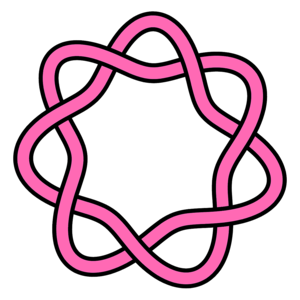
\includegraphics[width=\linewidth]{../data/knots/7_1.png}
        \subcaption{$7_{1}$}
    \end{minipage}
    \begin{minipage}[b]{.18\linewidth}
        \centering
        
\includegraphics[width=\linewidth]{../data/knots/7_2.png}
        \subcaption{$7_{2}$}
    \end{minipage}
    \begin{minipage}[b]{.18\linewidth}
        \centering
        
\includegraphics[width=\linewidth]{../data/knots/7_3.png}
        \subcaption{$7_{3}$}
    \end{minipage}
\end{figure}
\begin{figure}[H]
    \begin{minipage}[b]{.18\linewidth}
        \centering
        
\includegraphics[width=\linewidth]{../data/knots/7_4.png}
        \subcaption{$7_{4}$}
    \end{minipage}
    \begin{minipage}[b]{.18\linewidth}
        \centering
        
\includegraphics[width=\linewidth]{../data/knots/7_5.png}
        \subcaption{$7_{5}$}
    \end{minipage}
    \begin{minipage}[b]{.18\linewidth}
        \centering
        
\includegraphics[width=\linewidth]{../data/knots/7_6.png}
        \subcaption{$7_{6}$}
    \end{minipage}
    \begin{minipage}[b]{.18\linewidth}
        \centering
        
\includegraphics[width=\linewidth]{../data/knots/7_7.png}
        \subcaption{$7_{7}$}
    \end{minipage}
    \begin{minipage}[b]{.18\linewidth}
        \centering
        
\includegraphics[width=\linewidth]{../data/knots/8_1.png}
        \subcaption{$8_{1}$}
    \end{minipage}
\end{figure}
\begin{figure}[H]
    \begin{minipage}[b]{.18\linewidth}
        \centering
        
\includegraphics[width=\linewidth]{../data/knots/8_2.png}
        \subcaption{$8_{2}$}
    \end{minipage}
    \begin{minipage}[b]{.18\linewidth}
        \centering
        
\includegraphics[width=\linewidth]{../data/knots/8_3.png}
        \subcaption{$8_{3}$}
    \end{minipage}
    \begin{minipage}[b]{.18\linewidth}
        \centering
        
\includegraphics[width=\linewidth]{../data/knots/8_4.png}
        \subcaption{$8_{4}$}
    \end{minipage}
    \begin{minipage}[b]{.18\linewidth}
        \centering
        
\includegraphics[width=\linewidth]{../data/knots/8_5.png}
        \subcaption{$8_{5}$}
    \end{minipage}
    \begin{minipage}[b]{.18\linewidth}
        \centering
        
\includegraphics[width=\linewidth]{../data/knots/8_6.png}
        \subcaption{$8_{6}$}
    \end{minipage}
\end{figure}
\begin{figure}[H]
    \begin{minipage}[b]{.18\linewidth}
        \centering
        
\includegraphics[width=\linewidth]{../data/knots/8_7.png}
        \subcaption{$8_{7}$}
    \end{minipage}
    \begin{minipage}[b]{.18\linewidth}
        \centering
        
\includegraphics[width=\linewidth]{../data/knots/8_8.png}
        \subcaption{$8_{8}$}
    \end{minipage}
    \begin{minipage}[b]{.18\linewidth}
        \centering
        
\includegraphics[width=\linewidth]{../data/knots/8_9.png}
        \subcaption{$8_{9}$}
    \end{minipage}
    \begin{minipage}[b]{.18\linewidth}
        \centering
        
\includegraphics[width=\linewidth]{../data/knots/8_10.png}
        \subcaption{$8_{10}$}
    \end{minipage}
    \begin{minipage}[b]{.18\linewidth}
        \centering
        \includegraphics[width=\linewidth]{../data/knots/8_11.png}
        \subcaption{$8_{11}$}
    \end{minipage}
\end{figure}
\begin{figure}[H]
    \begin{minipage}[b]{.18\linewidth}
        \centering
        \includegraphics[width=\linewidth]{../data/knots/8_12.png}
        \subcaption{$8_{12}$}
    \end{minipage}
    \begin{minipage}[b]{.18\linewidth}
        \centering
        \includegraphics[width=\linewidth]{../data/knots/8_13.png}
        \subcaption{$8_{13}$}
    \end{minipage}
    \begin{minipage}[b]{.18\linewidth}
        \centering
        \includegraphics[width=\linewidth]{../data/knots/8_14.png}
        \subcaption{$8_{14}$}
    \end{minipage}
    \begin{minipage}[b]{.18\linewidth}
        \centering
        \includegraphics[width=\linewidth]{../data/knots/8_15.png}
        \subcaption{$8_{15}$}
    \end{minipage}
    \begin{minipage}[b]{.18\linewidth}
        \centering
        \includegraphics[width=\linewidth]{../data/knots/8_16.png}
        \subcaption{$8_{16}$}
    \end{minipage}
\end{figure}
\begin{figure}[H]
    \begin{minipage}[b]{.18\linewidth}
        \centering
        \includegraphics[width=\linewidth]{../data/knots/8_17.png}
        \subcaption{$8_{17}$}
    \end{minipage}
    \begin{minipage}[b]{.18\linewidth}
        \centering
        \includegraphics[width=\linewidth]{../data/knots/8_18.png}
        \subcaption{$8_{18}$}
    \end{minipage}
    \begin{minipage}[b]{.18\linewidth}
        \centering
        \includegraphics[width=\linewidth]{../data/knots/8_19.png}
        \subcaption{$8_{19}$}
    \end{minipage}
    \begin{minipage}[b]{.18\linewidth}
        \centering
        \includegraphics[width=\linewidth]{../data/knots/8_20.png}
        \subcaption{$8_{20}$}
    \end{minipage}
    \begin{minipage}[b]{.18\linewidth}
        \centering
        \includegraphics[width=\linewidth]{../data/knots/8_21.png}
        \subcaption{$8_{21}$}
    \end{minipage}
\end{figure}
\begin{figure}[H]
    \begin{minipage}[b]{.18\linewidth}
        \centering
        \includegraphics[width=\linewidth]{../data/knots/9_1.png}
        \subcaption{$9_{1}$}
    \end{minipage}
    \begin{minipage}[b]{.18\linewidth}
        \centering
        \includegraphics[width=\linewidth]{../data/knots/9_2.png}
        \subcaption{$9_{2}$}
    \end{minipage}
    \begin{minipage}[b]{.18\linewidth}
        \centering
        \includegraphics[width=\linewidth]{../data/knots/9_3.png}
        \subcaption{$9_{3}$}
    \end{minipage}
    \begin{minipage}[b]{.18\linewidth}
        \centering
        \includegraphics[width=\linewidth]{../data/knots/9_4.png}
        \subcaption{$9_{4}$}
    \end{minipage}
    \begin{minipage}[b]{.18\linewidth}
        \centering
        \includegraphics[width=\linewidth]{../data/knots/9_5.png}
        \subcaption{$9_{5}$}
    \end{minipage}
\end{figure}
\begin{figure}[H]
    \begin{minipage}[b]{.18\linewidth}
        \centering
        \includegraphics[width=\linewidth]{../data/knots/9_6.png}
        \subcaption{$9_{6}$}
    \end{minipage}
    \begin{minipage}[b]{.18\linewidth}
        \centering
        \includegraphics[width=\linewidth]{../data/knots/9_7.png}
        \subcaption{$9_{7}$}
    \end{minipage}
    \begin{minipage}[b]{.18\linewidth}
        \centering
        \includegraphics[width=\linewidth]{../data/knots/9_8.png}
        \subcaption{$9_{8}$}
    \end{minipage}
    \begin{minipage}[b]{.18\linewidth}
        \centering
        \includegraphics[width=\linewidth]{../data/knots/9_9.png}
        \subcaption{$9_{9}$}
    \end{minipage}
    \begin{minipage}[b]{.18\linewidth}
        \centering
        \includegraphics[width=\linewidth]{../data/knots/9_10.png}
        \subcaption{$9_{10}$}
    \end{minipage}
\end{figure}
\begin{figure}[H]
    \begin{minipage}[b]{.18\linewidth}
        \centering
        \includegraphics[width=\linewidth]{../data/knots/9_11.png}
        \subcaption{$9_{11}$}
    \end{minipage}
    \begin{minipage}[b]{.18\linewidth}
        \centering
        \includegraphics[width=\linewidth]{../data/knots/9_12.png}
        \subcaption{$9_{12}$}
    \end{minipage}
    \begin{minipage}[b]{.18\linewidth}
        \centering
        \includegraphics[width=\linewidth]{../data/knots/9_13.png}
        \subcaption{$9_{13}$}
    \end{minipage}
    \begin{minipage}[b]{.18\linewidth}
        \centering
        \includegraphics[width=\linewidth]{../data/knots/9_14.png}
        \subcaption{$9_{14}$}
    \end{minipage}
    \begin{minipage}[b]{.18\linewidth}
        \centering
        \includegraphics[width=\linewidth]{../data/knots/9_15.png}
        \subcaption{$9_{15}$}
    \end{minipage}
\end{figure}
\begin{figure}[H]
    \begin{minipage}[b]{.18\linewidth}
        \centering
        \includegraphics[width=\linewidth]{../data/knots/9_16.png}
        \subcaption{$9_{16}$}
    \end{minipage}
    \begin{minipage}[b]{.18\linewidth}
        \centering
        \includegraphics[width=\linewidth]{../data/knots/9_17.png}
        \subcaption{$9_{17}$}
    \end{minipage}
    \begin{minipage}[b]{.18\linewidth}
        \centering
        \includegraphics[width=\linewidth]{../data/knots/9_18.png}
        \subcaption{$9_{18}$}
    \end{minipage}
    \begin{minipage}[b]{.18\linewidth}
        \centering
        \includegraphics[width=\linewidth]{../data/knots/9_19.png}
        \subcaption{$9_{19}$}
    \end{minipage}
    \begin{minipage}[b]{.18\linewidth}
        \centering
        \includegraphics[width=\linewidth]{../data/knots/9_20.png}
        \subcaption{$9_{20}$}
    \end{minipage}
\end{figure}
\begin{figure}[H]
    \begin{minipage}[b]{.18\linewidth}
        \centering
        \includegraphics[width=\linewidth]{../data/knots/9_21.png}
        \subcaption{$9_{21}$}
    \end{minipage}
    \begin{minipage}[b]{.18\linewidth}
        \centering
        \includegraphics[width=\linewidth]{../data/knots/9_22.png}
        \subcaption{$9_{22}$}
    \end{minipage}
    \begin{minipage}[b]{.18\linewidth}
        \centering
        \includegraphics[width=\linewidth]{../data/knots/9_23.png}
        \subcaption{$9_{23}$}
    \end{minipage}
    \begin{minipage}[b]{.18\linewidth}
        \centering
        \includegraphics[width=\linewidth]{../data/knots/9_24.png}
        \subcaption{$9_{24}$}
    \end{minipage}
    \begin{minipage}[b]{.18\linewidth}
        \centering
        \includegraphics[width=\linewidth]{../data/knots/9_25.png}
        \subcaption{$9_{25}$}
    \end{minipage}
\end{figure}
\begin{figure}[H]
    \begin{minipage}[b]{.18\linewidth}
        \centering
        \includegraphics[width=\linewidth]{../data/knots/9_26.png}
        \subcaption{$9_{26}$}
    \end{minipage}
    \begin{minipage}[b]{.18\linewidth}
        \centering
        \includegraphics[width=\linewidth]{../data/knots/9_27.png}
        \subcaption{$9_{27}$}
    \end{minipage}
    \begin{minipage}[b]{.18\linewidth}
        \centering
        \includegraphics[width=\linewidth]{../data/knots/9_28.png}
        \subcaption{$9_{28}$}
    \end{minipage}
    \begin{minipage}[b]{.18\linewidth}
        \centering
        \includegraphics[width=\linewidth]{../data/knots/9_29.png}
        \subcaption{$9_{29}$}
    \end{minipage}
    \begin{minipage}[b]{.18\linewidth}
        \centering
        \includegraphics[width=\linewidth]{../data/knots/9_30.png}
        \subcaption{$9_{30}$}
    \end{minipage}
\end{figure}
\begin{figure}[H]
    \begin{minipage}[b]{.18\linewidth}
        \centering
        \includegraphics[width=\linewidth]{../data/knots/9_31.png}
        \subcaption{$9_{31}$}
    \end{minipage}
    \begin{minipage}[b]{.18\linewidth}
        \centering
        \includegraphics[width=\linewidth]{../data/knots/9_32.png}
        \subcaption{$9_{32}$}
    \end{minipage}
    \begin{minipage}[b]{.18\linewidth}
        \centering
        \includegraphics[width=\linewidth]{../data/knots/9_33.png}
        \subcaption{$9_{33}$}
    \end{minipage}
    \begin{minipage}[b]{.18\linewidth}
        \centering
        \includegraphics[width=\linewidth]{../data/knots/9_34.png}
        \subcaption{$9_{34}$}
    \end{minipage}
    \begin{minipage}[b]{.18\linewidth}
        \centering
        \includegraphics[width=\linewidth]{../data/knots/9_35.png}
        \subcaption{$9_{35}$}
    \end{minipage}
\end{figure}
\begin{figure}[H]
    \begin{minipage}[b]{.18\linewidth}
        \centering
        \includegraphics[width=\linewidth]{../data/knots/9_36.png}
        \subcaption{$9_{36}$}
    \end{minipage}
    \begin{minipage}[b]{.18\linewidth}
        \centering
        \includegraphics[width=\linewidth]{../data/knots/9_37.png}
        \subcaption{$9_{37}$}
    \end{minipage}
    \begin{minipage}[b]{.18\linewidth}
        \centering
        \includegraphics[width=\linewidth]{../data/knots/9_38.png}
        \subcaption{$9_{38}$}
    \end{minipage}
    \begin{minipage}[b]{.18\linewidth}
        \centering
        \includegraphics[width=\linewidth]{../data/knots/9_39.png}
        \subcaption{$9_{39}$}
    \end{minipage}
    \begin{minipage}[b]{.18\linewidth}
        \centering
        \includegraphics[width=\linewidth]{../data/knots/9_40.png}
        \subcaption{$9_{40}$}
    \end{minipage}
\end{figure}
\begin{figure}[H]
    \begin{minipage}[b]{.18\linewidth}
        \centering
        \includegraphics[width=\linewidth]{../data/knots/9_41.png}
        \subcaption{$9_{41}$}
    \end{minipage}
    \begin{minipage}[b]{.18\linewidth}
        \centering
        \includegraphics[width=\linewidth]{../data/knots/9_42.png}
        \subcaption{$9_{42}$}
    \end{minipage}
    \begin{minipage}[b]{.18\linewidth}
        \centering
        \includegraphics[width=\linewidth]{../data/knots/9_43.png}
        \subcaption{$9_{43}$}
    \end{minipage}
    \begin{minipage}[b]{.18\linewidth}
        \centering
        \includegraphics[width=\linewidth]{../data/knots/9_44.png}
        \subcaption{$9_{44}$}
    \end{minipage}
    \begin{minipage}[b]{.18\linewidth}
        \centering
        \includegraphics[width=\linewidth]{../data/knots/9_45.png}
        \subcaption{$9_{45}$}
    \end{minipage}
\end{figure}
\begin{figure}[H]
    \begin{minipage}[b]{.18\linewidth}
        \centering
        \includegraphics[width=\linewidth]{../data/knots/9_46.png}
        \subcaption{$9_{46}$}
    \end{minipage}
    \begin{minipage}[b]{.18\linewidth}
        \centering
        \includegraphics[width=\linewidth]{../data/knots/9_47.png}
        \subcaption{$9_{47}$}
    \end{minipage}
    \begin{minipage}[b]{.18\linewidth}
        \centering
        \includegraphics[width=\linewidth]{../data/knots/9_48.png}
        \subcaption{$9_{48}$}
    \end{minipage}
    \begin{minipage}[b]{.18\linewidth}
        \centering
        \includegraphics[width=\linewidth]{../data/knots/9_49.png}
        \subcaption{$9_{49}$}
    \end{minipage}
    \begin{minipage}[b]{.18\linewidth}
        \centering
        \includegraphics[width=\linewidth]{../data/knots/10_1.png}
        \subcaption{$10_{1}$}
    \end{minipage}
\end{figure}
\begin{figure}[H]
    \begin{minipage}[b]{.18\linewidth}
        \centering
        \includegraphics[width=\linewidth]{../data/knots/10_2.png}
        \subcaption{$10_{2}$}
    \end{minipage}
    \begin{minipage}[b]{.18\linewidth}
        \centering
        \includegraphics[width=\linewidth]{../data/knots/10_3.png}
        \subcaption{$10_{3}$}
    \end{minipage}
    \begin{minipage}[b]{.18\linewidth}
        \centering
        \includegraphics[width=\linewidth]{../data/knots/10_4.png}
        \subcaption{$10_{4}$}
    \end{minipage}
    \begin{minipage}[b]{.18\linewidth}
        \centering
        \includegraphics[width=\linewidth]{../data/knots/10_5.png}
        \subcaption{$10_{5}$}
    \end{minipage}
    \begin{minipage}[b]{.18\linewidth}
        \centering
        \includegraphics[width=\linewidth]{../data/knots/10_6.png}
        \subcaption{$10_{6}$}
    \end{minipage}
\end{figure}
\begin{figure}[H]
    \begin{minipage}[b]{.18\linewidth}
        \centering
        \includegraphics[width=\linewidth]{../data/knots/10_7.png}
        \subcaption{$10_{7}$}
    \end{minipage}
    \begin{minipage}[b]{.18\linewidth}
        \centering
        \includegraphics[width=\linewidth]{../data/knots/10_8.png}
        \subcaption{$10_{8}$}
    \end{minipage}
    \begin{minipage}[b]{.18\linewidth}
        \centering
        \includegraphics[width=\linewidth]{../data/knots/10_9.png}
        \subcaption{$10_{9}$}
    \end{minipage}
    \begin{minipage}[b]{.18\linewidth}
        \centering
        \includegraphics[width=\linewidth]{../data/knots/10_10.png}
        \subcaption{$10_{10}$}
    \end{minipage}
    \begin{minipage}[b]{.18\linewidth}
        \centering
        \includegraphics[width=\linewidth]{../data/knots/10_11.png}
        \subcaption{$10_{11}$}
    \end{minipage}
\end{figure}
\begin{figure}[H]
    \begin{minipage}[b]{.18\linewidth}
        \centering
        \includegraphics[width=\linewidth]{../data/knots/10_12.png}
        \subcaption{$10_{12}$}
    \end{minipage}
    \begin{minipage}[b]{.18\linewidth}
        \centering
        \includegraphics[width=\linewidth]{../data/knots/10_13.png}
        \subcaption{$10_{13}$}
    \end{minipage}
    \begin{minipage}[b]{.18\linewidth}
        \centering
        \includegraphics[width=\linewidth]{../data/knots/10_14.png}
        \subcaption{$10_{14}$}
    \end{minipage}
    \begin{minipage}[b]{.18\linewidth}
        \centering
        \includegraphics[width=\linewidth]{../data/knots/10_15.png}
        \subcaption{$10_{15}$}
    \end{minipage}
    \begin{minipage}[b]{.18\linewidth}
        \centering
        \includegraphics[width=\linewidth]{../data/knots/10_16.png}
        \subcaption{$10_{16}$}
    \end{minipage}
\end{figure}
\begin{figure}[H]
    \begin{minipage}[b]{.18\linewidth}
        \centering
        \includegraphics[width=\linewidth]{../data/knots/10_17.png}
        \subcaption{$10_{17}$}
    \end{minipage}
    \begin{minipage}[b]{.18\linewidth}
        \centering
        \includegraphics[width=\linewidth]{../data/knots/10_18.png}
        \subcaption{$10_{18}$}
    \end{minipage}
    \begin{minipage}[b]{.18\linewidth}
        \centering
        \includegraphics[width=\linewidth]{../data/knots/10_19.png}
        \subcaption{$10_{19}$}
    \end{minipage}
    \begin{minipage}[b]{.18\linewidth}
        \centering
        \includegraphics[width=\linewidth]{../data/knots/10_20.png}
        \subcaption{$10_{20}$}
    \end{minipage}
    \begin{minipage}[b]{.18\linewidth}
        \centering
        \includegraphics[width=\linewidth]{../data/knots/10_21.png}
        \subcaption{$10_{21}$}
    \end{minipage}
\end{figure}
\begin{figure}[H]
    \begin{minipage}[b]{.18\linewidth}
        \centering
        \includegraphics[width=\linewidth]{../data/knots/10_22.png}
        \subcaption{$10_{22}$}
    \end{minipage}
    \begin{minipage}[b]{.18\linewidth}
        \centering
        \includegraphics[width=\linewidth]{../data/knots/10_23.png}
        \subcaption{$10_{23}$}
    \end{minipage}
    \begin{minipage}[b]{.18\linewidth}
        \centering
        \includegraphics[width=\linewidth]{../data/knots/10_24.png}
        \subcaption{$10_{24}$}
    \end{minipage}
    \begin{minipage}[b]{.18\linewidth}
        \centering
        \includegraphics[width=\linewidth]{../data/knots/10_25.png}
        \subcaption{$10_{25}$}
    \end{minipage}
    \begin{minipage}[b]{.18\linewidth}
        \centering
        \includegraphics[width=\linewidth]{../data/knots/10_26.png}
        \subcaption{$10_{26}$}
    \end{minipage}
\end{figure}
\begin{figure}[H]
    \begin{minipage}[b]{.18\linewidth}
        \centering
        \includegraphics[width=\linewidth]{../data/knots/10_27.png}
        \subcaption{$10_{27}$}
    \end{minipage}
    \begin{minipage}[b]{.18\linewidth}
        \centering
        \includegraphics[width=\linewidth]{../data/knots/10_28.png}
        \subcaption{$10_{28}$}
    \end{minipage}
    \begin{minipage}[b]{.18\linewidth}
        \centering
        \includegraphics[width=\linewidth]{../data/knots/10_29.png}
        \subcaption{$10_{29}$}
    \end{minipage}
    \begin{minipage}[b]{.18\linewidth}
        \centering
        \includegraphics[width=\linewidth]{../data/knots/10_30.png}
        \subcaption{$10_{30}$}
    \end{minipage}
    \begin{minipage}[b]{.18\linewidth}
        \centering
        \includegraphics[width=\linewidth]{../data/knots/10_31.png}
        \subcaption{$10_{31}$}
    \end{minipage}
\end{figure}
\begin{figure}[H]
    \begin{minipage}[b]{.18\linewidth}
        \centering
        \includegraphics[width=\linewidth]{../data/knots/10_32.png}
        \subcaption{$10_{32}$}
    \end{minipage}
    \begin{minipage}[b]{.18\linewidth}
        \centering
        \includegraphics[width=\linewidth]{../data/knots/10_33.png}
        \subcaption{$10_{33}$}
    \end{minipage}
    \begin{minipage}[b]{.18\linewidth}
        \centering
        \includegraphics[width=\linewidth]{../data/knots/10_34.png}
        \subcaption{$10_{34}$}
    \end{minipage}
    \begin{minipage}[b]{.18\linewidth}
        \centering
        \includegraphics[width=\linewidth]{../data/knots/10_35.png}
        \subcaption{$10_{35}$}
    \end{minipage}
    \begin{minipage}[b]{.18\linewidth}
        \centering
        \includegraphics[width=\linewidth]{../data/knots/10_36.png}
        \subcaption{$10_{36}$}
    \end{minipage}
\end{figure}
\begin{figure}[H]
    \begin{minipage}[b]{.18\linewidth}
        \centering
        \includegraphics[width=\linewidth]{../data/knots/10_37.png}
        \subcaption{$10_{37}$}
    \end{minipage}
    \begin{minipage}[b]{.18\linewidth}
        \centering
        \includegraphics[width=\linewidth]{../data/knots/10_38.png}
        \subcaption{$10_{38}$}
    \end{minipage}
    \begin{minipage}[b]{.18\linewidth}
        \centering
        \includegraphics[width=\linewidth]{../data/knots/10_39.png}
        \subcaption{$10_{39}$}
    \end{minipage}
    \begin{minipage}[b]{.18\linewidth}
        \centering
        \includegraphics[width=\linewidth]{../data/knots/10_40.png}
        \subcaption{$10_{40}$}
    \end{minipage}
    \begin{minipage}[b]{.18\linewidth}
        \centering
        \includegraphics[width=\linewidth]{../data/knots/10_41.png}
        \subcaption{$10_{41}$}
    \end{minipage}
\end{figure}
\begin{figure}[H]
    \begin{minipage}[b]{.18\linewidth}
        \centering
        \includegraphics[width=\linewidth]{../data/knots/10_42.png}
        \subcaption{$10_{42}$}
    \end{minipage}
    \begin{minipage}[b]{.18\linewidth}
        \centering
        \includegraphics[width=\linewidth]{../data/knots/10_43.png}
        \subcaption{$10_{43}$}
    \end{minipage}
    \begin{minipage}[b]{.18\linewidth}
        \centering
        \includegraphics[width=\linewidth]{../data/knots/10_44.png}
        \subcaption{$10_{44}$}
    \end{minipage}
    \begin{minipage}[b]{.18\linewidth}
        \centering
        \includegraphics[width=\linewidth]{../data/knots/10_45.png}
        \subcaption{$10_{45}$}
    \end{minipage}
    \begin{minipage}[b]{.18\linewidth}
        \centering
        \includegraphics[width=\linewidth]{../data/knots/10_46.png}
        \subcaption{$10_{46}$}
    \end{minipage}
\end{figure}
\begin{figure}[H]
    \begin{minipage}[b]{.18\linewidth}
        \centering
        \includegraphics[width=\linewidth]{../data/knots/10_47.png}
        \subcaption{$10_{47}$}
    \end{minipage}
    \begin{minipage}[b]{.18\linewidth}
        \centering
        \includegraphics[width=\linewidth]{../data/knots/10_48.png}
        \subcaption{$10_{48}$}
    \end{minipage}
    \begin{minipage}[b]{.18\linewidth}
        \centering
        \includegraphics[width=\linewidth]{../data/knots/10_49.png}
        \subcaption{$10_{49}$}
    \end{minipage}
    \begin{minipage}[b]{.18\linewidth}
        \centering
        \includegraphics[width=\linewidth]{../data/knots/10_50.png}
        \subcaption{$10_{50}$}
    \end{minipage}
    \begin{minipage}[b]{.18\linewidth}
        \centering
        \includegraphics[width=\linewidth]{../data/knots/10_51.png}
        \subcaption{$10_{51}$}
    \end{minipage}
\end{figure}
\begin{figure}[H]
    \begin{minipage}[b]{.18\linewidth}
        \centering
        \includegraphics[width=\linewidth]{../data/knots/10_52.png}
        \subcaption{$10_{52}$}
    \end{minipage}
    \begin{minipage}[b]{.18\linewidth}
        \centering
        \includegraphics[width=\linewidth]{../data/knots/10_53.png}
        \subcaption{$10_{53}$}
    \end{minipage}
    \begin{minipage}[b]{.18\linewidth}
        \centering
        \includegraphics[width=\linewidth]{../data/knots/10_54.png}
        \subcaption{$10_{54}$}
    \end{minipage}
    \begin{minipage}[b]{.18\linewidth}
        \centering
        \includegraphics[width=\linewidth]{../data/knots/10_55.png}
        \subcaption{$10_{55}$}
    \end{minipage}
    \begin{minipage}[b]{.18\linewidth}
        \centering
        \includegraphics[width=\linewidth]{../data/knots/10_56.png}
        \subcaption{$10_{56}$}
    \end{minipage}
\end{figure}
\begin{figure}[H]
    \begin{minipage}[b]{.18\linewidth}
        \centering
        \includegraphics[width=\linewidth]{../data/knots/10_57.png}
        \subcaption{$10_{57}$}
    \end{minipage}
    \begin{minipage}[b]{.18\linewidth}
        \centering
        \includegraphics[width=\linewidth]{../data/knots/10_58.png}
        \subcaption{$10_{58}$}
    \end{minipage}
    \begin{minipage}[b]{.18\linewidth}
        \centering
        \includegraphics[width=\linewidth]{../data/knots/10_59.png}
        \subcaption{$10_{59}$}
    \end{minipage}
    \begin{minipage}[b]{.18\linewidth}
        \centering
        \includegraphics[width=\linewidth]{../data/knots/10_60.png}
        \subcaption{$10_{60}$}
    \end{minipage}
    \begin{minipage}[b]{.18\linewidth}
        \centering
        \includegraphics[width=\linewidth]{../data/knots/10_61.png}
        \subcaption{$10_{61}$}
    \end{minipage}
\end{figure}
\begin{figure}[H]
    \begin{minipage}[b]{.18\linewidth}
        \centering
        \includegraphics[width=\linewidth]{../data/knots/10_62.png}
        \subcaption{$10_{62}$}
    \end{minipage}
    \begin{minipage}[b]{.18\linewidth}
        \centering
        \includegraphics[width=\linewidth]{../data/knots/10_63.png}
        \subcaption{$10_{63}$}
    \end{minipage}
    \begin{minipage}[b]{.18\linewidth}
        \centering
        \includegraphics[width=\linewidth]{../data/knots/10_64.png}
        \subcaption{$10_{64}$}
    \end{minipage}
    \begin{minipage}[b]{.18\linewidth}
        \centering
        \includegraphics[width=\linewidth]{../data/knots/10_65.png}
        \subcaption{$10_{65}$}
    \end{minipage}
    \begin{minipage}[b]{.18\linewidth}
        \centering
        \includegraphics[width=\linewidth]{../data/knots/10_66.png}
        \subcaption{$10_{66}$}
    \end{minipage}
\end{figure}
\begin{figure}[H]
    \begin{minipage}[b]{.18\linewidth}
        \centering
        \includegraphics[width=\linewidth]{../data/knots/10_67.png}
        \subcaption{$10_{67}$}
    \end{minipage}
    \begin{minipage}[b]{.18\linewidth}
        \centering
        \includegraphics[width=\linewidth]{../data/knots/10_68.png}
        \subcaption{$10_{68}$}
    \end{minipage}
    \begin{minipage}[b]{.18\linewidth}
        \centering
        \includegraphics[width=\linewidth]{../data/knots/10_69.png}
        \subcaption{$10_{69}$}
    \end{minipage}
    \begin{minipage}[b]{.18\linewidth}
        \centering
        \includegraphics[width=\linewidth]{../data/knots/10_70.png}
        \subcaption{$10_{70}$}
    \end{minipage}
    \begin{minipage}[b]{.18\linewidth}
        \centering
        \includegraphics[width=\linewidth]{../data/knots/10_71.png}
        \subcaption{$10_{71}$}
    \end{minipage}
\end{figure}
\begin{figure}[H]
    \begin{minipage}[b]{.18\linewidth}
        \centering
        \includegraphics[width=\linewidth]{../data/knots/10_72.png}
        \subcaption{$10_{72}$}
    \end{minipage}
    \begin{minipage}[b]{.18\linewidth}
        \centering
        \includegraphics[width=\linewidth]{../data/knots/10_73.png}
        \subcaption{$10_{73}$}
    \end{minipage}
    \begin{minipage}[b]{.18\linewidth}
        \centering
        \includegraphics[width=\linewidth]{../data/knots/10_74.png}
        \subcaption{$10_{74}$}
    \end{minipage}
    \begin{minipage}[b]{.18\linewidth}
        \centering
        \includegraphics[width=\linewidth]{../data/knots/10_75.png}
        \subcaption{$10_{75}$}
    \end{minipage}
    \begin{minipage}[b]{.18\linewidth}
        \centering
        \includegraphics[width=\linewidth]{../data/knots/10_76.png}
        \subcaption{$10_{76}$}
    \end{minipage}
\end{figure}
\begin{figure}[H]
    \begin{minipage}[b]{.18\linewidth}
        \centering
        \includegraphics[width=\linewidth]{../data/knots/10_77.png}
        \subcaption{$10_{77}$}
    \end{minipage}
    \begin{minipage}[b]{.18\linewidth}
        \centering
        \includegraphics[width=\linewidth]{../data/knots/10_78.png}
        \subcaption{$10_{78}$}
    \end{minipage}
    \begin{minipage}[b]{.18\linewidth}
        \centering
        \includegraphics[width=\linewidth]{../data/knots/10_79.png}
        \subcaption{$10_{79}$}
    \end{minipage}
    \begin{minipage}[b]{.18\linewidth}
        \centering
        \includegraphics[width=\linewidth]{../data/knots/10_80.png}
        \subcaption{$10_{80}$}
    \end{minipage}
    \begin{minipage}[b]{.18\linewidth}
        \centering
        \includegraphics[width=\linewidth]{../data/knots/10_81.png}
        \subcaption{$10_{81}$}
    \end{minipage}
\end{figure}
\begin{figure}[H]
    \begin{minipage}[b]{.18\linewidth}
        \centering
        \includegraphics[width=\linewidth]{../data/knots/10_82.png}
        \subcaption{$10_{82}$}
    \end{minipage}
    \begin{minipage}[b]{.18\linewidth}
        \centering
        \includegraphics[width=\linewidth]{../data/knots/10_83.png}
        \subcaption{$10_{83}$}
    \end{minipage}
    \begin{minipage}[b]{.18\linewidth}
        \centering
        \includegraphics[width=\linewidth]{../data/knots/10_84.png}
        \subcaption{$10_{84}$}
    \end{minipage}
    \begin{minipage}[b]{.18\linewidth}
        \centering
        \includegraphics[width=\linewidth]{../data/knots/10_85.png}
        \subcaption{$10_{85}$}
    \end{minipage}
    \begin{minipage}[b]{.18\linewidth}
        \centering
        \includegraphics[width=\linewidth]{../data/knots/10_86.png}
        \subcaption{$10_{86}$}
    \end{minipage}
\end{figure}
\begin{figure}[H]
    \begin{minipage}[b]{.18\linewidth}
        \centering
        \includegraphics[width=\linewidth]{../data/knots/10_87.png}
        \subcaption{$10_{87}$}
    \end{minipage}
    \begin{minipage}[b]{.18\linewidth}
        \centering
        \includegraphics[width=\linewidth]{../data/knots/10_88.png}
        \subcaption{$10_{88}$}
    \end{minipage}
    \begin{minipage}[b]{.18\linewidth}
        \centering
        \includegraphics[width=\linewidth]{../data/knots/10_89.png}
        \subcaption{$10_{89}$}
    \end{minipage}
    \begin{minipage}[b]{.18\linewidth}
        \centering
        \includegraphics[width=\linewidth]{../data/knots/10_90.png}
        \subcaption{$10_{90}$}
    \end{minipage}
    \begin{minipage}[b]{.18\linewidth}
        \centering
        \includegraphics[width=\linewidth]{../data/knots/10_91.png}
        \subcaption{$10_{91}$}
    \end{minipage}
\end{figure}
\begin{figure}[H]
    \begin{minipage}[b]{.18\linewidth}
        \centering
        \includegraphics[width=\linewidth]{../data/knots/10_92.png}
        \subcaption{$10_{92}$}
    \end{minipage}
    \begin{minipage}[b]{.18\linewidth}
        \centering
        \includegraphics[width=\linewidth]{../data/knots/10_93.png}
        \subcaption{$10_{93}$}
    \end{minipage}
    \begin{minipage}[b]{.18\linewidth}
        \centering
        \includegraphics[width=\linewidth]{../data/knots/10_94.png}
        \subcaption{$10_{94}$}
    \end{minipage}
    \begin{minipage}[b]{.18\linewidth}
        \centering
        \includegraphics[width=\linewidth]{../data/knots/10_95.png}
        \subcaption{$10_{95}$}
    \end{minipage}
    \begin{minipage}[b]{.18\linewidth}
        \centering
        \includegraphics[width=\linewidth]{../data/knots/10_96.png}
        \subcaption{$10_{96}$}
    \end{minipage}
\end{figure}
\begin{figure}[H]
    \begin{minipage}[b]{.18\linewidth}
        \centering
        \includegraphics[width=\linewidth]{../data/knots/10_97.png}
        \subcaption{$10_{97}$}
    \end{minipage}
    \begin{minipage}[b]{.18\linewidth}
        \centering
        \includegraphics[width=\linewidth]{../data/knots/10_98.png}
        \subcaption{$10_{98}$}
    \end{minipage}
    \begin{minipage}[b]{.18\linewidth}
        \centering
        \includegraphics[width=\linewidth]{../data/knots/10_99.png}
        \subcaption{$10_{99}$}
    \end{minipage}
    \begin{minipage}[b]{.18\linewidth}
        \centering
        \includegraphics[width=\linewidth]{../data/knots/10_100.png}
        \subcaption{$10_{100}$}
    \end{minipage}
    \begin{minipage}[b]{.18\linewidth}
        \centering
        \includegraphics[width=\linewidth]{../data/knots/10_101.png}
        \subcaption{$10_{101}$}
    \end{minipage}
\end{figure}
\begin{figure}[H]
    \begin{minipage}[b]{.18\linewidth}
        \centering
        \includegraphics[width=\linewidth]{../data/knots/10_102.png}
        \subcaption{$10_{102}$}
    \end{minipage}
    \begin{minipage}[b]{.18\linewidth}
        \centering
        \includegraphics[width=\linewidth]{../data/knots/10_103.png}
        \subcaption{$10_{103}$}
    \end{minipage}
    \begin{minipage}[b]{.18\linewidth}
        \centering
        \includegraphics[width=\linewidth]{../data/knots/10_104.png}
        \subcaption{$10_{104}$}
    \end{minipage}
    \begin{minipage}[b]{.18\linewidth}
        \centering
        \includegraphics[width=\linewidth]{../data/knots/10_105.png}
        \subcaption{$10_{105}$}
    \end{minipage}
    \begin{minipage}[b]{.18\linewidth}
        \centering
        \includegraphics[width=\linewidth]{../data/knots/10_106.png}
        \subcaption{$10_{106}$}
    \end{minipage}
\end{figure}
\begin{figure}[H]
    \begin{minipage}[b]{.18\linewidth}
        \centering
        \includegraphics[width=\linewidth]{../data/knots/10_107.png}
        \subcaption{$10_{107}$}
    \end{minipage}
    \begin{minipage}[b]{.18\linewidth}
        \centering
        \includegraphics[width=\linewidth]{../data/knots/10_108.png}
        \subcaption{$10_{108}$}
    \end{minipage}
    \begin{minipage}[b]{.18\linewidth}
        \centering
        \includegraphics[width=\linewidth]{../data/knots/10_109.png}
        \subcaption{$10_{109}$}
    \end{minipage}
    \begin{minipage}[b]{.18\linewidth}
        \centering
        \includegraphics[width=\linewidth]{../data/knots/10_110.png}
        \subcaption{$10_{110}$}
    \end{minipage}
    \begin{minipage}[b]{.18\linewidth}
        \centering
        \includegraphics[width=\linewidth]{../data/knots/10_111.png}
        \subcaption{$10_{111}$}
    \end{minipage}
\end{figure}
\begin{figure}[H]
    \begin{minipage}[b]{.18\linewidth}
        \centering
        \includegraphics[width=\linewidth]{../data/knots/10_112.png}
        \subcaption{$10_{112}$}
    \end{minipage}
    \begin{minipage}[b]{.18\linewidth}
        \centering
        \includegraphics[width=\linewidth]{../data/knots/10_113.png}
        \subcaption{$10_{113}$}
    \end{minipage}
    \begin{minipage}[b]{.18\linewidth}
        \centering
        \includegraphics[width=\linewidth]{../data/knots/10_114.png}
        \subcaption{$10_{114}$}
    \end{minipage}
    \begin{minipage}[b]{.18\linewidth}
        \centering
        \includegraphics[width=\linewidth]{../data/knots/10_115.png}
        \subcaption{$10_{115}$}
    \end{minipage}
    \begin{minipage}[b]{.18\linewidth}
        \centering
        \includegraphics[width=\linewidth]{../data/knots/10_116.png}
        \subcaption{$10_{116}$}
    \end{minipage}
\end{figure}
\begin{figure}[H]
    \begin{minipage}[b]{.18\linewidth}
        \centering
        \includegraphics[width=\linewidth]{../data/knots/10_117.png}
        \subcaption{$10_{117}$}
    \end{minipage}
    \begin{minipage}[b]{.18\linewidth}
        \centering
        \includegraphics[width=\linewidth]{../data/knots/10_118.png}
        \subcaption{$10_{118}$}
    \end{minipage}
    \begin{minipage}[b]{.18\linewidth}
        \centering
        \includegraphics[width=\linewidth]{../data/knots/10_119.png}
        \subcaption{$10_{119}$}
    \end{minipage}
    \begin{minipage}[b]{.18\linewidth}
        \centering
        \includegraphics[width=\linewidth]{../data/knots/10_120.png}
        \subcaption{$10_{120}$}
    \end{minipage}
    \begin{minipage}[b]{.18\linewidth}
        \centering
        \includegraphics[width=\linewidth]{../data/knots/10_121.png}
        \subcaption{$10_{121}$}
    \end{minipage}
\end{figure}
\begin{figure}[H]
    \begin{minipage}[b]{.18\linewidth}
        \centering
        \includegraphics[width=\linewidth]{../data/knots/10_122.png}
        \subcaption{$10_{122}$}
    \end{minipage}
    \begin{minipage}[b]{.18\linewidth}
        \centering
        \includegraphics[width=\linewidth]{../data/knots/10_123.png}
        \subcaption{$10_{123}$}
    \end{minipage}
    \begin{minipage}[b]{.18\linewidth}
        \centering
        \includegraphics[width=\linewidth]{../data/knots/10_124.png}
        \subcaption{$10_{124}$}
    \end{minipage}
    \begin{minipage}[b]{.18\linewidth}
        \centering
        \includegraphics[width=\linewidth]{../data/knots/10_125.png}
        \subcaption{$10_{125}$}
    \end{minipage}
    \begin{minipage}[b]{.18\linewidth}
        \centering
        \includegraphics[width=\linewidth]{../data/knots/10_126.png}
        \subcaption{$10_{126}$}
    \end{minipage}
\end{figure}
\begin{figure}[H]
    \begin{minipage}[b]{.18\linewidth}
        \centering
        \includegraphics[width=\linewidth]{../data/knots/10_127.png}
        \subcaption{$10_{127}$}
    \end{minipage}
    \begin{minipage}[b]{.18\linewidth}
        \centering
        \includegraphics[width=\linewidth]{../data/knots/10_128.png}
        \subcaption{$10_{128}$}
    \end{minipage}
    \begin{minipage}[b]{.18\linewidth}
        \centering
        \includegraphics[width=\linewidth]{../data/knots/10_129.png}
        \subcaption{$10_{129}$}
    \end{minipage}
    \begin{minipage}[b]{.18\linewidth}
        \centering
        \includegraphics[width=\linewidth]{../data/knots/10_130.png}
        \subcaption{$10_{130}$}
    \end{minipage}
    \begin{minipage}[b]{.18\linewidth}
        \centering
        \includegraphics[width=\linewidth]{../data/knots/10_131.png}
        \subcaption{$10_{131}$}
    \end{minipage}
\end{figure}
\begin{figure}[H]
    \begin{minipage}[b]{.18\linewidth}
        \centering
        \includegraphics[width=\linewidth]{../data/knots/10_132.png}
        \subcaption{$10_{132}$}
    \end{minipage}
    \begin{minipage}[b]{.18\linewidth}
        \centering
        \includegraphics[width=\linewidth]{../data/knots/10_133.png}
        \subcaption{$10_{133}$}
    \end{minipage}
    \begin{minipage}[b]{.18\linewidth}
        \centering
        \includegraphics[width=\linewidth]{../data/knots/10_134.png}
        \subcaption{$10_{134}$}
    \end{minipage}
    \begin{minipage}[b]{.18\linewidth}
        \centering
        \includegraphics[width=\linewidth]{../data/knots/10_135.png}
        \subcaption{$10_{135}$}
    \end{minipage}
    \begin{minipage}[b]{.18\linewidth}
        \centering
        \includegraphics[width=\linewidth]{../data/knots/10_136.png}
        \subcaption{$10_{136}$}
    \end{minipage}
\end{figure}
\begin{figure}[H]
    \begin{minipage}[b]{.18\linewidth}
        \centering
        \includegraphics[width=\linewidth]{../data/knots/10_137.png}
        \subcaption{$10_{137}$}
    \end{minipage}
    \begin{minipage}[b]{.18\linewidth}
        \centering
        \includegraphics[width=\linewidth]{../data/knots/10_138.png}
        \subcaption{$10_{138}$}
    \end{minipage}
    \begin{minipage}[b]{.18\linewidth}
        \centering
        \includegraphics[width=\linewidth]{../data/knots/10_139.png}
        \subcaption{$10_{139}$}
    \end{minipage}
    \begin{minipage}[b]{.18\linewidth}
        \centering
        \includegraphics[width=\linewidth]{../data/knots/10_140.png}
        \subcaption{$10_{140}$}
    \end{minipage}
    \begin{minipage}[b]{.18\linewidth}
        \centering
        \includegraphics[width=\linewidth]{../data/knots/10_141.png}
        \subcaption{$10_{141}$}
    \end{minipage}
\end{figure}
\begin{figure}[H]
    \begin{minipage}[b]{.18\linewidth}
        \centering
        \includegraphics[width=\linewidth]{../data/knots/10_142.png}
        \subcaption{$10_{142}$}
    \end{minipage}
    \begin{minipage}[b]{.18\linewidth}
        \centering
        \includegraphics[width=\linewidth]{../data/knots/10_143.png}
        \subcaption{$10_{143}$}
    \end{minipage}
    \begin{minipage}[b]{.18\linewidth}
        \centering
        \includegraphics[width=\linewidth]{../data/knots/10_144.png}
        \subcaption{$10_{144}$}
    \end{minipage}
    \begin{minipage}[b]{.18\linewidth}
        \centering
        \includegraphics[width=\linewidth]{../data/knots/10_145.png}
        \subcaption{$10_{145}$}
    \end{minipage}
    \begin{minipage}[b]{.18\linewidth}
        \centering
        \includegraphics[width=\linewidth]{../data/knots/10_146.png}
        \subcaption{$10_{146}$}
    \end{minipage}
\end{figure}
\begin{figure}[H]
    \begin{minipage}[b]{.18\linewidth}
        \centering
        \includegraphics[width=\linewidth]{../data/knots/10_147.png}
        \subcaption{$10_{147}$}
    \end{minipage}
    \begin{minipage}[b]{.18\linewidth}
        \centering
        \includegraphics[width=\linewidth]{../data/knots/10_148.png}
        \subcaption{$10_{148}$}
    \end{minipage}
    \begin{minipage}[b]{.18\linewidth}
        \centering
        \includegraphics[width=\linewidth]{../data/knots/10_149.png}
        \subcaption{$10_{149}$}
    \end{minipage}
    \begin{minipage}[b]{.18\linewidth}
        \centering
        \includegraphics[width=\linewidth]{../data/knots/10_150.png}
        \subcaption{$10_{150}$}
    \end{minipage}
    \begin{minipage}[b]{.18\linewidth}
        \centering
        \includegraphics[width=\linewidth]{../data/knots/10_151.png}
        \subcaption{$10_{151}$}
    \end{minipage}
\end{figure}
\begin{figure}[H]
    \begin{minipage}[b]{.18\linewidth}
        \centering
        \includegraphics[width=\linewidth]{../data/knots/10_152.png}
        \subcaption{$10_{152}$}
    \end{minipage}
    \begin{minipage}[b]{.18\linewidth}
        \centering
        \includegraphics[width=\linewidth]{../data/knots/10_153.png}
        \subcaption{$10_{153}$}
    \end{minipage}
    \begin{minipage}[b]{.18\linewidth}
        \centering
        \includegraphics[width=\linewidth]{../data/knots/10_154.png}
        \subcaption{$10_{154}$}
    \end{minipage}
    \begin{minipage}[b]{.18\linewidth}
        \centering
        \includegraphics[width=\linewidth]{../data/knots/10_155.png}
        \subcaption{$10_{155}$}
    \end{minipage}
    \begin{minipage}[b]{.18\linewidth}
        \centering
        \includegraphics[width=\linewidth]{../data/knots/10_156.png}
        \subcaption{$10_{156}$}
    \end{minipage}
\end{figure}
\begin{figure}[H]
    \begin{minipage}[b]{.18\linewidth}
        \centering
        \includegraphics[width=\linewidth]{../data/knots/10_157.png}
        \subcaption{$10_{157}$}
    \end{minipage}
    \begin{minipage}[b]{.18\linewidth}
        \centering
        \includegraphics[width=\linewidth]{../data/knots/10_158.png}
        \subcaption{$10_{158}$}
    \end{minipage}
    \begin{minipage}[b]{.18\linewidth}
        \centering
        \includegraphics[width=\linewidth]{../data/knots/10_159.png}
        \subcaption{$10_{159}$}
    \end{minipage}
    \begin{minipage}[b]{.18\linewidth}
        \centering
        \includegraphics[width=\linewidth]{../data/knots/10_160.png}
        \subcaption{$10_{160}$}
    \end{minipage}
    \begin{minipage}[b]{.18\linewidth}
        \centering
        \includegraphics[width=\linewidth]{../data/knots/10_161.png}
        \subcaption{$10_{161}$}
    \end{minipage}
\end{figure}
\begin{figure}[H]
    \begin{minipage}[b]{.18\linewidth}
        \centering
        \includegraphics[width=\linewidth]{../data/knots/10_162.png}
        \subcaption{$10_{162}$}
    \end{minipage}
    \begin{minipage}[b]{.18\linewidth}
        \centering
        \includegraphics[width=\linewidth]{../data/knots/10_163.png}
        \subcaption{$10_{163}$}
    \end{minipage}
    \begin{minipage}[b]{.18\linewidth}
        \centering
        \includegraphics[width=\linewidth]{../data/knots/10_164.png}
        \subcaption{$10_{164}$}
    \end{minipage}
    \begin{minipage}[b]{.18\linewidth}
        \centering
        \includegraphics[width=\linewidth]{../data/knots/10_165.png}
        \subcaption{$10_{165}$}
    \end{minipage}
\end{figure}
\end{comment}



    \chapter{Tablice splotów}
    
\section{Diagramy splotów pierwszych do dziewięciu skrzyżowań}
% Poniżej znajdują się diagramy węzłów pierwszych, które realizują liczbę gordyjską, jeśli ta nie przekracza dziesięciu.
% One także pochodzą ze strony KnotInfo \cite{knotinfo2024}, o~której mowa na początku rozdziału.
Coś o LinkInfo...
% TODO

\begin{comment}
\begin{figure}[H]
    \begin{minipage}[b]{.18\linewidth}
        \centering
        \includegraphics[width=\linewidth]{../data/links/2_2_1.png}
        \subcaption{$2^2_{1} = L_2a_{1}$}
    \end{minipage}
    \begin{minipage}[b]{.18\linewidth}
        \centering
        \includegraphics[width=\linewidth]{../data/links/4_2_1.png}
        \subcaption{$4^2_{1} = L_4a_{1}$}
    \end{minipage}
    \begin{minipage}[b]{.18\linewidth}
        \centering
        \includegraphics[width=\linewidth]{../data/links/5_2_1.png}
        \subcaption{$5^2_{1} = L_5a_{1}$}
    \end{minipage}
    \begin{minipage}[b]{.18\linewidth}
        \centering
        \includegraphics[width=\linewidth]{../data/links/6_2_1.png}
        \subcaption{$6^2_{1} = L_6a_{3}$}
    \end{minipage}
    \begin{minipage}[b]{.18\linewidth}
        \centering
        \includegraphics[width=\linewidth]{../data/links/6_2_2.png}
        \subcaption{$6^2_{2} = L_6a_{2}$}
    \end{minipage}
\end{figure}
\begin{figure}[H]
    \begin{minipage}[b]{.18\linewidth}
        \centering
        \includegraphics[width=\linewidth]{../data/links/6_2_3.png}
        \subcaption{$6^2_{3} = L_6a_{1}$}
    \end{minipage}
    \begin{minipage}[b]{.18\linewidth}
        \centering
        \includegraphics[width=\linewidth]{../data/links/6_3_1.png}
        \subcaption{$6^3_{1} = L_6a_{5}$}
    \end{minipage}
    \begin{minipage}[b]{.18\linewidth}
        \centering
        \includegraphics[width=\linewidth]{../data/links/6_3_2.png}
        \subcaption{$6^3_{2} = L_6a_{4}$}
    \end{minipage}
    \begin{minipage}[b]{.18\linewidth}
        \centering
        \includegraphics[width=\linewidth]{../data/links/6_3_3.png}
        \subcaption{$6^3_{3} = L_6n_{1}$}
    \end{minipage}
    \begin{minipage}[b]{.18\linewidth}
        \centering
        \includegraphics[width=\linewidth]{../data/links/7_2_1.png}
        \subcaption{$7^2_{1} = L_7a_{6}$}
    \end{minipage}
\end{figure}
\begin{figure}[H]
    \begin{minipage}[b]{.18\linewidth}
        \centering
        \includegraphics[width=\linewidth]{../data/links/7_2_2.png}
        \subcaption{$7^2_{2} = L_7a_{5}$}
    \end{minipage}
    \begin{minipage}[b]{.18\linewidth}
        \centering
        \includegraphics[width=\linewidth]{../data/links/7_2_3.png}
        \subcaption{$7^2_{3} = L_7a_{4}$}
    \end{minipage}
    \begin{minipage}[b]{.18\linewidth}
        \centering
        \includegraphics[width=\linewidth]{../data/links/7_2_4.png}
        \subcaption{$7^2_{4} = L_7a_{3}$}
    \end{minipage}
    \begin{minipage}[b]{.18\linewidth}
        \centering
        \includegraphics[width=\linewidth]{../data/links/7_2_5.png}
        \subcaption{$7^2_{5} = L_7a_{2}$}
    \end{minipage}
    \begin{minipage}[b]{.18\linewidth}
        \centering
        \includegraphics[width=\linewidth]{../data/links/7_2_6.png}
        \subcaption{$7^2_{6} = L_7a_{1}$}
    \end{minipage}
\end{figure}
\begin{figure}[H]
    \begin{minipage}[b]{.18\linewidth}
        \centering
        \includegraphics[width=\linewidth]{../data/links/7_2_7.png}
        \subcaption{$7^2_{7} = L_7n_{1}$}
    \end{minipage}
    \begin{minipage}[b]{.18\linewidth}
        \centering
        \includegraphics[width=\linewidth]{../data/links/7_2_8.png}
        \subcaption{$7^2_{8} = L_7n_{2}$}
    \end{minipage}
    \begin{minipage}[b]{.18\linewidth}
        \centering
        \includegraphics[width=\linewidth]{../data/links/7_3_1.png}
        \subcaption{$7^3_{1} = L_7a_{7}$}
    \end{minipage}
    \begin{minipage}[b]{.18\linewidth}
        \centering
        \includegraphics[width=\linewidth]{../data/links/8_2_1.png}
        \subcaption{$8^2_{1} = L_8a_{14}$}
    \end{minipage}
    \begin{minipage}[b]{.18\linewidth}
        \centering
        \includegraphics[width=\linewidth]{../data/links/8_2_2.png}
        \subcaption{$8^2_{2} = L_8a_{12}$}
    \end{minipage}
\end{figure}
\begin{figure}[H]
    \begin{minipage}[b]{.18\linewidth}
        \centering
        \includegraphics[width=\linewidth]{../data/links/8_2_3.png}
        \subcaption{$8^2_{3} = L_8a_{11}$}
    \end{minipage}
    \begin{minipage}[b]{.18\linewidth}
        \centering
        \includegraphics[width=\linewidth]{../data/links/8_2_4.png}
        \subcaption{$8^2_{4} = L_8a_{13}$}
    \end{minipage}
    \begin{minipage}[b]{.18\linewidth}
        \centering
        \includegraphics[width=\linewidth]{../data/links/8_2_5.png}
        \subcaption{$8^2_{5} = L_8a_{10}$}
    \end{minipage}
    \begin{minipage}[b]{.18\linewidth}
        \centering
        \includegraphics[width=\linewidth]{../data/links/8_2_6.png}
        \subcaption{$8^2_{6} = L_8a_{6}$}
    \end{minipage}
    \begin{minipage}[b]{.18\linewidth}
        \centering
        \includegraphics[width=\linewidth]{../data/links/8_2_7.png}
        \subcaption{$8^2_{7} = L_8a_{8}$}
    \end{minipage}
\end{figure}
\begin{figure}[H]
    \begin{minipage}[b]{.18\linewidth}
        \centering
        \includegraphics[width=\linewidth]{../data/links/8_2_8.png}
        \subcaption{$8^2_{8} = L_8a_{9}$}
    \end{minipage}
    \begin{minipage}[b]{.18\linewidth}
        \centering
        \includegraphics[width=\linewidth]{../data/links/8_2_9.png}
        \subcaption{$8^2_{9} = L_8a_{3}$}
    \end{minipage}
    \begin{minipage}[b]{.18\linewidth}
        \centering
        \includegraphics[width=\linewidth]{../data/links/8_2_10.png}
        \subcaption{$8^2_{10} = L_8a_{2}$}
    \end{minipage}
    \begin{minipage}[b]{.18\linewidth}
        \centering
        \includegraphics[width=\linewidth]{../data/links/8_2_11.png}
        \subcaption{$8^2_{11} = L_8a_{5}$}
    \end{minipage}
    \begin{minipage}[b]{.18\linewidth}
        \centering
        \includegraphics[width=\linewidth]{../data/links/8_2_12.png}
        \subcaption{$8^2_{12} = L_8a_{4}$}
    \end{minipage}
\end{figure}
\begin{figure}[H]
    \begin{minipage}[b]{.18\linewidth}
        \centering
        \includegraphics[width=\linewidth]{../data/links/8_2_13.png}
        \subcaption{$8^2_{13} = L_8a_{1}$}
    \end{minipage}
    \begin{minipage}[b]{.18\linewidth}
        \centering
        \includegraphics[width=\linewidth]{../data/links/8_2_14.png}
        \subcaption{$8^2_{14} = L_8a_{7}$}
    \end{minipage}
    \begin{minipage}[b]{.18\linewidth}
        \centering
        \includegraphics[width=\linewidth]{../data/links/8_2_15.png}
        \subcaption{$8^2_{15} = L_8n_{2}$}
    \end{minipage}
    \begin{minipage}[b]{.18\linewidth}
        \centering
        \includegraphics[width=\linewidth]{../data/links/8_2_16.png}
        \subcaption{$8^2_{16} = L_8n_{1}$}
    \end{minipage}
    \begin{minipage}[b]{.18\linewidth}
        \centering
        \includegraphics[width=\linewidth]{../data/links/8_3_1.png}
        \subcaption{$8^3_{1} = L_8a_{18}$}
    \end{minipage}
\end{figure}
\begin{figure}[H]
    \begin{minipage}[b]{.18\linewidth}
        \centering
        \includegraphics[width=\linewidth]{../data/links/8_3_2.png}
        \subcaption{$8^3_{2} = L_8a_{17}$}
    \end{minipage}
    \begin{minipage}[b]{.18\linewidth}
        \centering
        \includegraphics[width=\linewidth]{../data/links/8_3_3.png}
        \subcaption{$8^3_{3} = L_8a_{15}$}
    \end{minipage}
    \begin{minipage}[b]{.18\linewidth}
        \centering
        \includegraphics[width=\linewidth]{../data/links/8_3_4.png}
        \subcaption{$8^3_{4} = L_8a_{20}$}
    \end{minipage}
    \begin{minipage}[b]{.18\linewidth}
        \centering
        \includegraphics[width=\linewidth]{../data/links/8_3_5.png}
        \subcaption{$8^3_{5} = L_8a_{16}$}
    \end{minipage}
    \begin{minipage}[b]{.18\linewidth}
        \centering
        \includegraphics[width=\linewidth]{../data/links/8_3_6.png}
        \subcaption{$8^3_{6} = L_8a_{19}$}
    \end{minipage}
\end{figure}
\begin{figure}[H]
    \begin{minipage}[b]{.18\linewidth}
        \centering
        \includegraphics[width=\linewidth]{../data/links/8_3_7.png}
        \subcaption{$8^3_{7} = L_8n_{3}$}
    \end{minipage}
    \begin{minipage}[b]{.18\linewidth}
        \centering
        \includegraphics[width=\linewidth]{../data/links/8_3_8.png}
        \subcaption{$8^3_{8} = L_8n_{4}$}
    \end{minipage}
    \begin{minipage}[b]{.18\linewidth}
        \centering
        \includegraphics[width=\linewidth]{../data/links/8_3_9.png}
        \subcaption{$8^3_{9} = L_8n_{5}$}
    \end{minipage}
    \begin{minipage}[b]{.18\linewidth}
        \centering
        \includegraphics[width=\linewidth]{../data/links/8_3_10.png}
        \subcaption{$8^3_{10} = L_8n_{6}$}
    \end{minipage}
    \begin{minipage}[b]{.18\linewidth}
        \centering
        \includegraphics[width=\linewidth]{../data/links/8_4_1.png}
        \subcaption{$8^4_{1} = L_8a_{21}$}
    \end{minipage}
\end{figure}
\begin{figure}[H]
    \begin{minipage}[b]{.18\linewidth}
        \centering
        \includegraphics[width=\linewidth]{../data/links/8_4_2.png}
        \subcaption{$8^4_{2} = L_8n_{7}$}
    \end{minipage}
    \begin{minipage}[b]{.18\linewidth}
        \centering
        \includegraphics[width=\linewidth]{../data/links/8_4_3.png}
        \subcaption{$8^4_{3} = L_8n_{8}$}
    \end{minipage}
    \begin{minipage}[b]{.18\linewidth}
        \centering
        \includegraphics[width=\linewidth]{../data/links/9_2_1.png}
        \subcaption{$9^2_{1} = L_9a_{36}$}
    \end{minipage}
    \begin{minipage}[b]{.18\linewidth}
        \centering
        \includegraphics[width=\linewidth]{../data/links/9_2_2.png}
        \subcaption{$9^2_{2} = L_9a_{39}$}
    \end{minipage}
    \begin{minipage}[b]{.18\linewidth}
        \centering
        \includegraphics[width=\linewidth]{../data/links/9_2_3.png}
        \subcaption{$9^2_{3} = L_9a_{30}$}
    \end{minipage}
\end{figure}
\begin{figure}[H]
    \begin{minipage}[b]{.18\linewidth}
        \centering
        \includegraphics[width=\linewidth]{../data/links/9_2_4.png}
        \subcaption{$9^2_{4} = L_9a_{40}$}
    \end{minipage}
    \begin{minipage}[b]{.18\linewidth}
        \centering
        \includegraphics[width=\linewidth]{../data/links/9_2_5.png}
        \subcaption{$9^2_{5} = L_9a_{38}$}
    \end{minipage}
    \begin{minipage}[b]{.18\linewidth}
        \centering
        \includegraphics[width=\linewidth]{../data/links/9_2_6.png}
        \subcaption{$9^2_{6} = L_9a_{34}$}
    \end{minipage}
    \begin{minipage}[b]{.18\linewidth}
        \centering
        \includegraphics[width=\linewidth]{../data/links/9_2_7.png}
        \subcaption{$9^2_{7} = L_9a_{37}$}
    \end{minipage}
    \begin{minipage}[b]{.18\linewidth}
        \centering
        \includegraphics[width=\linewidth]{../data/links/9_2_8.png}
        \subcaption{$9^2_{8} = L_9a_{25}$}
    \end{minipage}
\end{figure}
\begin{figure}[H]
    \begin{minipage}[b]{.18\linewidth}
        \centering
        \includegraphics[width=\linewidth]{../data/links/9_2_9.png}
        \subcaption{$9^2_{9} = L_9a_{35}$}
    \end{minipage}
    \begin{minipage}[b]{.18\linewidth}
        \centering
        \includegraphics[width=\linewidth]{../data/links/9_2_10.png}
        \subcaption{$9^2_{10} = L_9a_{18}$}
    \end{minipage}
    \begin{minipage}[b]{.18\linewidth}
        \centering
        \includegraphics[width=\linewidth]{../data/links/9_2_11.png}
        \subcaption{$9^2_{11} = L_9a_{26}$}
    \end{minipage}
    \begin{minipage}[b]{.18\linewidth}
        \centering
        \includegraphics[width=\linewidth]{../data/links/9_2_12.png}
        \subcaption{$9^2_{12} = L_9a_{27}$}
    \end{minipage}
    \begin{minipage}[b]{.18\linewidth}
        \centering
        \includegraphics[width=\linewidth]{../data/links/9_2_13.png}
        \subcaption{$9^2_{13} = L_9a_{14}$}
    \end{minipage}
\end{figure}
\begin{figure}[H]
    \begin{minipage}[b]{.18\linewidth}
        \centering
        \includegraphics[width=\linewidth]{../data/links/9_2_14.png}
        \subcaption{$9^2_{14} = L_9a_{12}$}
    \end{minipage}
    \begin{minipage}[b]{.18\linewidth}
        \centering
        \includegraphics[width=\linewidth]{../data/links/9_2_15.png}
        \subcaption{$9^2_{15} = L_9a_{15}$}
    \end{minipage}
    \begin{minipage}[b]{.18\linewidth}
        \centering
        \includegraphics[width=\linewidth]{../data/links/9_2_16.png}
        \subcaption{$9^2_{16} = L_9a_{13}$}
    \end{minipage}
    \begin{minipage}[b]{.18\linewidth}
        \centering
        \includegraphics[width=\linewidth]{../data/links/9_2_17.png}
        \subcaption{$9^2_{17} = L_9a_{7}$}
    \end{minipage}
    \begin{minipage}[b]{.18\linewidth}
        \centering
        \includegraphics[width=\linewidth]{../data/links/9_2_18.png}
        \subcaption{$9^2_{18} = L_9a_{4}$}
    \end{minipage}
\end{figure}
\begin{figure}[H]
    \begin{minipage}[b]{.18\linewidth}
        \centering
        \includegraphics[width=\linewidth]{../data/links/9_2_19.png}
        \subcaption{$9^2_{19} = L_9a_{29}$}
    \end{minipage}
    \begin{minipage}[b]{.18\linewidth}
        \centering
        \includegraphics[width=\linewidth]{../data/links/9_2_20.png}
        \subcaption{$9^2_{20} = L_9a_{28}$}
    \end{minipage}
    \begin{minipage}[b]{.18\linewidth}
        \centering
        \includegraphics[width=\linewidth]{../data/links/9_2_21.png}
        \subcaption{$9^2_{21} = L_9a_{24}$}
    \end{minipage}
    \begin{minipage}[b]{.18\linewidth}
        \centering
        \includegraphics[width=\linewidth]{../data/links/9_2_22.png}
        \subcaption{$9^2_{22} = L_9a_{23}$}
    \end{minipage}
    \begin{minipage}[b]{.18\linewidth}
        \centering
        \includegraphics[width=\linewidth]{../data/links/9_2_23.png}
        \subcaption{$9^2_{23} = L_9a_{41}$}
    \end{minipage}
\end{figure}
\begin{figure}[H]
    \begin{minipage}[b]{.18\linewidth}
        \centering
        \includegraphics[width=\linewidth]{../data/links/9_2_24.png}
        \subcaption{$9^2_{24} = L_9a_{33}$}
    \end{minipage}
    \begin{minipage}[b]{.18\linewidth}
        \centering
        \includegraphics[width=\linewidth]{../data/links/9_2_25.png}
        \subcaption{$9^2_{25} = L_9a_{8}$}
    \end{minipage}
    \begin{minipage}[b]{.18\linewidth}
        \centering
        \includegraphics[width=\linewidth]{../data/links/9_2_26.png}
        \subcaption{$9^2_{26} = L_9a_{11}$}
    \end{minipage}
    \begin{minipage}[b]{.18\linewidth}
        \centering
        \includegraphics[width=\linewidth]{../data/links/9_2_27.png}
        \subcaption{$9^2_{27} = L_9a_{17}$}
    \end{minipage}
    \begin{minipage}[b]{.18\linewidth}
        \centering
        \includegraphics[width=\linewidth]{../data/links/9_2_28.png}
        \subcaption{$9^2_{28} = L_9a_{16}$}
    \end{minipage}
\end{figure}
\begin{figure}[H]
    \begin{minipage}[b]{.18\linewidth}
        \centering
        \includegraphics[width=\linewidth]{../data/links/9_2_29.png}
        \subcaption{$9^2_{29} = L_9a_{6}$}
    \end{minipage}
    \begin{minipage}[b]{.18\linewidth}
        \centering
        \includegraphics[width=\linewidth]{../data/links/9_2_30.png}
        \subcaption{$9^2_{30} = L_9a_{5}$}
    \end{minipage}
    \begin{minipage}[b]{.18\linewidth}
        \centering
        \includegraphics[width=\linewidth]{../data/links/9_2_31.png}
        \subcaption{$9^2_{31} = L_9a_{2}$}
    \end{minipage}
    \begin{minipage}[b]{.18\linewidth}
        \centering
        \includegraphics[width=\linewidth]{../data/links/9_2_32.png}
        \subcaption{$9^2_{32} = L_9a_{1}$}
    \end{minipage}
    \begin{minipage}[b]{.18\linewidth}
        \centering
        \includegraphics[width=\linewidth]{../data/links/9_2_33.png}
        \subcaption{$9^2_{33} = L_9a_{3}$}
    \end{minipage}
\end{figure}
\begin{figure}[H]
    \begin{minipage}[b]{.18\linewidth}
        \centering
        \includegraphics[width=\linewidth]{../data/links/9_2_34.png}
        \subcaption{$9^2_{34} = L_9a_{21}$}
    \end{minipage}
    \begin{minipage}[b]{.18\linewidth}
        \centering
        \includegraphics[width=\linewidth]{../data/links/9_2_35.png}
        \subcaption{$9^2_{35} = L_9a_{22}$}
    \end{minipage}
    \begin{minipage}[b]{.18\linewidth}
        \centering
        \includegraphics[width=\linewidth]{../data/links/9_2_36.png}
        \subcaption{$9^2_{36} = L_9a_{10}$}
    \end{minipage}
    \begin{minipage}[b]{.18\linewidth}
        \centering
        \includegraphics[width=\linewidth]{../data/links/9_2_37.png}
        \subcaption{$9^2_{37} = L_9a_{9}$}
    \end{minipage}
    \begin{minipage}[b]{.18\linewidth}
        \centering
        \includegraphics[width=\linewidth]{../data/links/9_2_38.png}
        \subcaption{$9^2_{38} = L_9a_{19}$}
    \end{minipage}
\end{figure}
\begin{figure}[H]
    \begin{minipage}[b]{.18\linewidth}
        \centering
        \includegraphics[width=\linewidth]{../data/links/9_2_39.png}
        \subcaption{$9^2_{39} = L_9a_{31}$}
    \end{minipage}
    \begin{minipage}[b]{.18\linewidth}
        \centering
        \includegraphics[width=\linewidth]{../data/links/9_2_40.png}
        \subcaption{$9^2_{40} = L_9a_{32}$}
    \end{minipage}
    \begin{minipage}[b]{.18\linewidth}
        \centering
        \includegraphics[width=\linewidth]{../data/links/9_2_41.png}
        \subcaption{$9^2_{41} = L_9a_{42}$}
    \end{minipage}
    \begin{minipage}[b]{.18\linewidth}
        \centering
        \includegraphics[width=\linewidth]{../data/links/9_2_42.png}
        \subcaption{$9^2_{42} = L_9a_{20}$}
    \end{minipage}
    \begin{minipage}[b]{.18\linewidth}
        \centering
        \includegraphics[width=\linewidth]{../data/links/9_2_43.png}
        \subcaption{$9^2_{43} = L_9n_{4}$}
    \end{minipage}
\end{figure}
\begin{figure}[H]
    \begin{minipage}[b]{.18\linewidth}
        \centering
        \includegraphics[width=\linewidth]{../data/links/9_2_44.png}
        \subcaption{$9^2_{44} = L_9n_{5}$}
    \end{minipage}
    \begin{minipage}[b]{.18\linewidth}
        \centering
        \includegraphics[width=\linewidth]{../data/links/9_2_45.png}
        \subcaption{$9^2_{45} = L_9n_{1}$}
    \end{minipage}
    \begin{minipage}[b]{.18\linewidth}
        \centering
        \includegraphics[width=\linewidth]{../data/links/9_2_46.png}
        \subcaption{$9^2_{46} = L_9n_{2}$}
    \end{minipage}
    \begin{minipage}[b]{.18\linewidth}
        \centering
        \includegraphics[width=\linewidth]{../data/links/9_2_47.png}
        \subcaption{$9^2_{47} = L_9n_{3}$}
    \end{minipage}
    \begin{minipage}[b]{.18\linewidth}
        \centering
        \includegraphics[width=\linewidth]{../data/links/9_2_48.png}
        \subcaption{$9^2_{48} = L_9n_{7}$}
    \end{minipage}
\end{figure}
\begin{figure}[H]
    \begin{minipage}[b]{.18\linewidth}
        \centering
        \includegraphics[width=\linewidth]{../data/links/9_2_49.png}
        \subcaption{$9^2_{49} = L_9n_{15}$}
    \end{minipage}
    \begin{minipage}[b]{.18\linewidth}
        \centering
        \includegraphics[width=\linewidth]{../data/links/9_2_50.png}
        \subcaption{$9^2_{50} = L_9n_{14}$}
    \end{minipage}
    \begin{minipage}[b]{.18\linewidth}
        \centering
        \includegraphics[width=\linewidth]{../data/links/9_2_51.png}
        \subcaption{$9^2_{51} = L_9n_{16}$}
    \end{minipage}
    \begin{minipage}[b]{.18\linewidth}
        \centering
        \includegraphics[width=\linewidth]{../data/links/9_2_52.png}
        \subcaption{$9^2_{52} = L_9n_{17}$}
    \end{minipage}
    \begin{minipage}[b]{.18\linewidth}
        \centering
        \includegraphics[width=\linewidth]{../data/links/9_2_53.png}
        \subcaption{$9^2_{53} = L_9n_{18}$}
    \end{minipage}
\end{figure}
\begin{figure}[H]
    \begin{minipage}[b]{.18\linewidth}
        \centering
        \includegraphics[width=\linewidth]{../data/links/9_2_54.png}
        \subcaption{$9^2_{54} = L_9n_{13}$}
    \end{minipage}
    \begin{minipage}[b]{.18\linewidth}
        \centering
        \includegraphics[width=\linewidth]{../data/links/9_2_55.png}
        \subcaption{$9^2_{55} = L_9n_{6}$}
    \end{minipage}
    \begin{minipage}[b]{.18\linewidth}
        \centering
        \includegraphics[width=\linewidth]{../data/links/9_2_56.png}
        \subcaption{$9^2_{56} = L_9n_{8}$}
    \end{minipage}
    \begin{minipage}[b]{.18\linewidth}
        \centering
        \includegraphics[width=\linewidth]{../data/links/9_2_57.png}
        \subcaption{$9^2_{57} = L_9n_{11}$}
    \end{minipage}
    \begin{minipage}[b]{.18\linewidth}
        \centering
        \includegraphics[width=\linewidth]{../data/links/9_2_58.png}
        \subcaption{$9^2_{58} = L_9n_{10}$}
    \end{minipage}
\end{figure}
\begin{figure}[H]
    \begin{minipage}[b]{.18\linewidth}
        \centering
        \includegraphics[width=\linewidth]{../data/links/9_2_59.png}
        \subcaption{$9^2_{59} = L_9n_{12}$}
    \end{minipage}
    \begin{minipage}[b]{.18\linewidth}
        \centering
        \includegraphics[width=\linewidth]{../data/links/9_2_60.png}
        \subcaption{$9^2_{60} = L_9n_{9}$}
    \end{minipage}
    \begin{minipage}[b]{.18\linewidth}
        \centering
        \includegraphics[width=\linewidth]{../data/links/9_2_61.png}
        \subcaption{$9^2_{61} = L_9n_{19}$}
    \end{minipage}
    \begin{minipage}[b]{.18\linewidth}
        \centering
        \includegraphics[width=\linewidth]{../data/links/9_3_1.png}
        \subcaption{$9^3_{1} = L_9a_{50}$}
    \end{minipage}
    \begin{minipage}[b]{.18\linewidth}
        \centering
        \includegraphics[width=\linewidth]{../data/links/9_3_2.png}
        \subcaption{$9^3_{2} = L_9a_{47}$}
    \end{minipage}
\end{figure}
\begin{figure}[H]
    \begin{minipage}[b]{.18\linewidth}
        \centering
        \includegraphics[width=\linewidth]{../data/links/9_3_3.png}
        \subcaption{$9^3_{3} = L_9a_{44}$}
    \end{minipage}
    \begin{minipage}[b]{.18\linewidth}
        \centering
        \includegraphics[width=\linewidth]{../data/links/9_3_4.png}
        \subcaption{$9^3_{4} = L_9a_{43}$}
    \end{minipage}
    \begin{minipage}[b]{.18\linewidth}
        \centering
        \includegraphics[width=\linewidth]{../data/links/9_3_5.png}
        \subcaption{$9^3_{5} = L_9a_{48}$}
    \end{minipage}
    \begin{minipage}[b]{.18\linewidth}
        \centering
        \includegraphics[width=\linewidth]{../data/links/9_3_6.png}
        \subcaption{$9^3_{6} = L_9a_{49}$}
    \end{minipage}
    \begin{minipage}[b]{.18\linewidth}
        \centering
        \includegraphics[width=\linewidth]{../data/links/9_3_7.png}
        \subcaption{$9^3_{7} = L_9a_{45}$}
    \end{minipage}
\end{figure}
\begin{figure}[H]
    \begin{minipage}[b]{.18\linewidth}
        \centering
        \includegraphics[width=\linewidth]{../data/links/9_3_8.png}
        \subcaption{$9^3_{8} = L_9a_{52}$}
    \end{minipage}
    \begin{minipage}[b]{.18\linewidth}
        \centering
        \includegraphics[width=\linewidth]{../data/links/9_3_9.png}
        \subcaption{$9^3_{9} = L_9a_{54}$}
    \end{minipage}
    \begin{minipage}[b]{.18\linewidth}
        \centering
        \includegraphics[width=\linewidth]{../data/links/9_3_10.png}
        \subcaption{$9^3_{10} = L_9a_{46}$}
    \end{minipage}
    \begin{minipage}[b]{.18\linewidth}
        \centering
        \includegraphics[width=\linewidth]{../data/links/9_3_11.png}
        \subcaption{$9^3_{11} = L_9a_{51}$}
    \end{minipage}
    \begin{minipage}[b]{.18\linewidth}
        \centering
        \includegraphics[width=\linewidth]{../data/links/9_3_12.png}
        \subcaption{$9^3_{12} = L_9a_{53}$}
    \end{minipage}
\end{figure}
\begin{figure}[H]
    \begin{minipage}[b]{.18\linewidth}
        \centering
        \includegraphics[width=\linewidth]{../data/links/9_3_13.png}
        \subcaption{$9^3_{13} = L_9n_{23}$}
    \end{minipage}
    \begin{minipage}[b]{.18\linewidth}
        \centering
        \includegraphics[width=\linewidth]{../data/links/9_3_14.png}
        \subcaption{$9^3_{14} = L_9n_{24}$}
    \end{minipage}
    \begin{minipage}[b]{.18\linewidth}
        \centering
        \includegraphics[width=\linewidth]{../data/links/9_3_15.png}
        \subcaption{$9^3_{15} = L_9n_{22}$}
    \end{minipage}
    \begin{minipage}[b]{.18\linewidth}
        \centering
        \includegraphics[width=\linewidth]{../data/links/9_3_16.png}
        \subcaption{$9^3_{16} = L_9n_{20}$}
    \end{minipage}
    \begin{minipage}[b]{.18\linewidth}
        \centering
        \includegraphics[width=\linewidth]{../data/links/9_3_17.png}
        \subcaption{$9^3_{17} = L_9n_{21}$}
    \end{minipage}
\end{figure}
\begin{figure}[H]
    \begin{minipage}[b]{.18\linewidth}
        \centering
        \includegraphics[width=\linewidth]{../data/links/9_3_18.png}
        \subcaption{$9^3_{18} = L_9n_{25}$}
    \end{minipage}
    \begin{minipage}[b]{.18\linewidth}
        \centering
        \includegraphics[width=\linewidth]{../data/links/9_3_19.png}
        \subcaption{$9^3_{19} = L_9n_{26}$}
    \end{minipage}
    \begin{minipage}[b]{.18\linewidth}
        \centering
        \includegraphics[width=\linewidth]{../data/links/9_3_20.png}
        \subcaption{$9^3_{20} = L_9n_{28}$}
    \end{minipage}
    \begin{minipage}[b]{.18\linewidth}
        \centering
        \includegraphics[width=\linewidth]{../data/links/9_3_21.png}
        \subcaption{$9^3_{21} = L_9n_{27}$}
    \end{minipage}
    \begin{minipage}[b]{.18\linewidth}
        \centering
        \includegraphics[width=\linewidth]{../data/links/9_4_1.png}
        \subcaption{$9^4_{1} = L_9a_{55}$}
    \end{minipage}
\end{figure}

\end{comment}



    \chapter{Notacja, użyte symbole}
    
Przez $\N, \Z, \Q, \R, \C$ oznaczamy kolejno zbiór liczb naturalnych (z~zerem lub bez, jak kto lubi), całkowitych, wymiernych, rzeczywistych i~wreszcie zespolonych.
$S^n$ oznacza $n$-sferę (i tak $S^1$ jest okręgiem, zaś $S^2$ powierzchnią trójwymiarowej kuli); $D^n$ to $n$-dysk.
Włożenie $A$ w $B$ to $A \hookrightarrow B$, ich izotopia to $A \cong B$.
Kratka ($\shrap$) oznacza sumę spójną.
Suma rozłączna $\sqcup$ tym różni się od teoriomnogościowej $\cup$, że składniki muszą być rozłączne. Obraz funkcji $f \colon X \to Y$ staramy się oznaczać $f[X]$, nie $f(X)$.
Lustro i~rewers węzła $K$ oznaczamy kolejno $\operatorname{m} K$ i~$\operatorname{r} K$.

Dla wielomianowych niezmienników stosujemy następujące symbole: $\alexander$, $\conway$, $\jones$, $P$, $F$, $Q$ dla wielomianu Alexandera, Conwaya, Jonesa, HOMFLY-PT, Kauffmana, BLM/Ho.
Wiele innych niezmienników ma krótkie, jednoliterowe oznaczenia.
I tak $\crossing, \braid, \bridge, \unknotting, \linking, \stick$ to kolejno: liczba/indeks skrzyżowaniowy, warkoczowy, mostowy, gordyjska, zaczepienia, patykowa.
$\sigma$ oznacza sygnaturę (Levine'a-Tristrama), $\det$ wyznacznik, $g, \chi$ genus i charakterystykę Eulera, $\operatorname{wr}$ spin, $\operatorname{lk}$ indeks zaczepienia, 
Rzadko, naprawdę rzadko, potrzebujemy czegoś dla liczby $p$-kolorowań, wybór pada zawsze na $\tau_p$.

% $$PSL(2, 7)$ to rzutowa specjalna grupa liniowa nad ciałem $F_7$.



    \chapter{Słownik angielsko-polski}
    \begin{compactitem}
    \item \textbf{braid, pure} warkocz, czysty
\item \textbf{braid} warkocz
\item \textbf{closure of braid} domknięcie warkocza
\item \textbf{pretzel link} splot preclowy, precel
\item \textbf{quandle} kwandel
\item \textbf{strand} pasmo
\item \textbf{tangle} supeł
\item \textbf{writhe} spin

    \end{compactitem}
\end{appendices}

\raggedright
\bibliographystyle{plain}
%\bibliographystyle{plunsrt}
\bibliography{knot_theory}

\newpage
\listoftodos[Lista rzeczy do poprawienia]
\end{document}
\end{document}